% \documentclass[a4paper,11pt, twoside]{article}
\documentclass[a4paper,11pt]{article}

% --- Packages essentiels ---
\usepackage[utf8]{inputenc} % Encodage UTF-8
\usepackage[T1]{fontenc}    % Encodage des polices
\usepackage[french]{babel}  % Support du français
\usepackage{lmodern}        % Polices de meilleure qualité
\usepackage{graphicx}       % Inclusion d'images
\usepackage{url}            % Gestion des URLs
\usepackage{amsmath,amssymb}% Symboles mathématiques avancés
\usepackage{tcolorbox}      % Boîtes colorées
\usepackage{makeidx}        % Création d'index
\usepackage{stmaryrd}       % Symboles mathématiques additionnels
\usepackage{mathtools}      % Outils mathématiques avancés
\usepackage{exsheets}       % Pour les exercices
\usepackage{wasysym,enumerate,bbm,xcolor,theorem,accents}
\usepackage{lipsum} % Pour générer du faux texte
\usepackage{fancyhdr} 

% --- Redéfinition des symboles < et > ---
\catcode`\<=\active \def<{
  \fontencoding{T1}\selectfont\symbol{60}\fontencoding{\encodingdefault}}
\catcode`\>=\active \def>{
  \fontencoding{T1}\selectfont\symbol{62}\fontencoding{\encodingdefault}}

% --- Commandes personnalisées ---
\newcommand{\assign}{:=}
\newcommand{\comma}{{,}}
\newcommand{\infixand}{\text{ and }}
\newcommand{\infixor}{\text{ or }}
\newcommand{\nequiv}{\mathrel{\not\equiv}}
\newcommand{\nin}{\notin}
\newcommand{\nobracket}{}
\newcommand{\nospace}{}
\newcommand{\textdots}{...}
\newcommand{\tmabbr}[1]{#1}
\newcommand{\tmaffiliation}[1]{\\ #1}
\newcommand{\tmcolor}[2]{{\color{#1}{#2}}}
\newcommand{\tmem}[1]{{\em #1\/}}
\newcommand{\tmmathbf}[1]{\ensuremath{\boldsymbol{#1}}}
\newcommand{\tmname}[1]{\textsc{#1}}
\newcommand{\tmop}[1]{\ensuremath{\operatorname{#1}}}
\newcommand{\tmrsub}[1]{\ensuremath{_{\textrm{#1}}}}
\newcommand{\tmrsup}[1]{\textsuperscript{#1}}
\newcommand{\tmscript}[1]{\text{\scriptsize{$#1$}}}
\newcommand{\tmstrong}[1]{\textbf{#1}}
\newcommand{\tmtextbf}[1]{\text{{\bfseries{#1}}}}
\newcommand{\tmtextit}[1]{\text{{\itshape{#1}}}}

\newenvironment{enumeratenumeric}{\begin{enumerate}[1.]}{\end{enumerate}}

\newcounter{nnacknowledgments}
\def\thennacknowledgments{\unskip}
\newcounter{tmcounter}
\newcommand{\custombinding}[1]{%
  \setcounter{tmcounter}{#1}%
  \addtocounter{tmcounter}{-1}%
  \refstepcounter{tmcounter}}
\usepackage[T3,T1]{fontenc}
\DeclareSymbolFont{tipa}{T3}{cmr}{m}{n}
\DeclareMathAccent{\invbreve}{\mathalpha}{tipa}{16}
\newcommand{\nonconverted}[1]{\mbox{}}

\linespread{1.3} % Interligne ajusté

% --- Création et réinitialisation du compteur pour les exercices ---
\newcounter{exercice}
\makeatletter
\@addtoreset{exercice}{part} % Réinitialise le compteur "exercice" à chaque nouvelle partie
\makeatother

% --- Définition de l'environnement "exercise" ---
\newenvironment{exercise}[1][]{%
  \refstepcounter{exercice}% Incrémente le compteur et permet la référence
  \addcontentsline{toc}{section}{Exercice \theexercice : #1}% Ajoute l'exercice à la TOC
  \begin{tcolorbox}[%
    title=Exercice \theexercice. #1,
    colback=blue!5,
    colframe=blue!75!black,
    fonttitle=\bfseries
  ]
}{%
  \end{tcolorbox}
}

% --- Affichage des sous-sections dans la table des matières ---
\setcounter{tocdepth}{2}



% --- Charger hyperref en dernier ---
\usepackage{hyperref}

\pagestyle{empty} 

\begin{document}
\pagenumbering{gobble} % désactive la numérotation temporairement

% --- Page de garde ---
\begin{center}
    \vspace*{0.1cm}
    
\includegraphics[width=0.3\textwidth]{figures/ENS_Logo_TL.jpg}\\[1cm]

    {\LARGE \textbf{Oraux ENS 2023-2024 :}}\\[1cm]
    {\LARGE \textbf{Recueil d'exercices et solutions complètes}}\\[1cm]

    {\Large Mathématiques — Filière MP}\\[2cm]

    {\Large Auteurs :}\\[0.5cm]
    {\large \textsc{SABIR Ilyass}}\\[0.3cm]
    {\large \textsc{ZINE Akram}}\\[0.3cm]
    {\large \textsc{ETTOUSY Badr}}\\[2cm]

    {\Large Avril 2024}
\end{center}
\newpage
\begin{center}
Oraux ENS 2023-2024 \\ 
SABIR Ilyass - ZINE Akram - ETTOUSY Badr
\end{center}

\newpage
\begin{center}
  \textbf{N.B.} : Si vous trouvez des erreurs de français ou de mathématiques, ou si vous avez des questions et/ou des suggestions,\\
  n'hésitez pas à nous contacter en envoyant un mail à :\\[0.2cm]
  \textbf{ilyass@steerai.autos} ou \textbf{ilyasssabir7@gmail.com}
\end{center}

\vspace{2cm}

\begin{center}
    Ce document a été relu par \textsc{SABIR Ilyass}, \textsc{ZINE Akram}, ainsi que d'autres personnes ayant vérifié certaines solutions.\\
    Un grand merci à tous les membres du groupe \textbf{Maths Community} pour leurs efforts dans la relecture de plusieurs parties de ce livre.
\end{center}

\vspace{1cm}

\begin{center}
  \textbf{Licence}
\end{center}

\begin{center}
  Ce document est sous licence \textbf{CC BY-NC-ND 4.0 DEED} :\\[0.2cm]
  \url{https://creativecommons.org/licenses/by-nc-nd/4.0/}\\[0.5cm]
  Tous droits réservés. Ce document et son contenu sont protégés par les lois sur le droit d'auteur.\\
  Toute reproduction, distribution ou utilisation des solutions présentées dans ce document\\
  à des fins commerciales nécessite une autorisation préalable.\\[0.5cm]
  
\includegraphics[width=3.5cm]{licence/Cc_by-nc-nd_euro_icon.svg.png}\\[0.3cm]
  \textbf{\copyright{} Paris, 2024}
\end{center}

\newpage
\section*{Avant-propos}
Ce recueil est bien plus qu'une simple collection d'exercices : il est conçu comme un compagnon de route pour tous les étudiants de prépa aspirant à intégrer les institutions les plus prestigieuses, telles que l’École normale supérieure (ENS) et l’École polytechnique (l’X), mais aussi pour les candidats des autres grandes écoles et concours de haut niveau. Les exercices rassemblés ici ne sont pas des problèmes standards : ils sont tirés d’épreuves orales réelles des concours des années précédentes, garantissant ainsi une immersion totale dans la réalité des défis à venir.

Le niveau de difficulté de chaque exercice peut varier selon l’étudiant, raison pour laquelle nous n’avons pas jugé utile de les classer selon ce critère. En effet, la difficulté perçue est une donnée subjective et dépend largement de votre maîtrise des sujets abordés. C’est pourquoi nous vous encourageons à aborder chaque exercice avec un esprit ouvert, prêt à explorer, à questionner et à approfondir vos connaissances. Nous vous recommandons également de travailler ces exercices dans des conditions aussi proches que possible de celles des oraux : une durée de 50 minutes pour les oraux d’ULM et de 45 minutes pour ceux du concours commun ULSR. Cela vous permettra non seulement de vous habituer à la gestion du temps, mais aussi de simuler l’environnement stressant des épreuves, où chaque minute compte et où la clarté de pensée est cruciale.

La variété des exercices dans ce recueil reflète les multiples facettes des mathématiques enseignées et évaluées lors des concours. Vous trouverez des problèmes d’algèbre, d’analyse, de géométrie, et même des défis en théorie des nombres. Certains exercices mettront à l’épreuve votre capacité à manipuler des objets classiques tels que les wronskiens, les séries alternées ou les matrices antisymétriques. D’autres vous amèneront à plonger plus profondément dans des problématiques actuelles, comme les espaces de translation ou les sous-groupes des isométries affines. Le but n’est pas simplement de résoudre ces problèmes, mais de comprendre les mécanismes sous-jacents qui permettent d’aborder des situations nouvelles avec confiance.

Pour vous soutenir dans cet effort, nous avons également inclus des solutions détaillées en annexe, qui couvrent non seulement les épreuves récentes de mathématiques A du concours X/ENS 2023 et 2024, mais aussi l’épreuve de mathématiques C du concours X/ENS 2018 et celle de l’agrégation externe de 2019. Ces solutions sont bien plus qu’une simple correction : elles vous guideront pas à pas dans le raisonnement et la méthodologie attendus au plus haut niveau.

En particulier, vous y trouverez une démonstration complète et rigoureuse du théorème de Dirichlet sur les progressions arithmétiques, un résultat fondamental qui revient régulièrement dans les concours. Cette démonstration, issue de l’épreuve ENS Paris-Lyon de 1993, est exposée avec minutie pour que chaque lecteur puisse en saisir tous les rouages, tant au niveau technique qu’intuitif.

En outre, nous vous invitons vivement à consulter les rapports des jurys des concours précédents. Ils vous permettront de mieux comprendre les attentes précises des examinateurs, les qualités qu’ils recherchent et les erreurs fréquentes à éviter. Enfin, en cas de difficulté, n’hésitez pas à recourir à des simplifications ou à des cas particuliers pour clarifier les concepts. Ce travail sur des versions plus abordables d’un problème peut souvent fournir des intuitions précieuses, vous permettant ensuite de revenir à l’énoncé général avec une meilleure compréhension.

La route vers l’excellence est exigeante, mais avec les bonnes méthodes et une persévérance inébranlable, elle est à votre portée. Nous espérons que ce recueil deviendra un compagnon de confiance dans cette aventure et vous aidera à aborder les oraux avec sérénité et confiance.

\bigskip

\noindent
Bonne préparation, et que vos efforts soient couronnés de succès.

\vspace{1cm}

\begin{flushright}
  \textbf{Les auteurs}
\end{flushright}


\newpage
\tableofcontents
\thispagestyle{empty}
\clearpage

\pagestyle{fancy}
\pagenumbering{arabic}
\setcounter{page}{1}

% En-têtes alternés pour pages impaires/paires
\fancyhf{}  % Efface tout
                     % Efface l’en-tête/pied existant
\fancyhead[L]{Oraux ENS 2023-2024}       % En-tête à gauche
\fancyhead[R]{\thepage}              % Numéro de page à droite
\renewcommand{\headrulewidth}{0.4pt} % Ligne sous l’en-tête

% \fancyhead[LO]{Oraux ENS 2023-2024}  % Left Odd (page impaire à gauche)
% \fancyhead[RE]{Oraux ENS 2023-2024}  % Right Even (page paire à droite)

% \fancyhead[RO]{\thepage}  % Right Odd (numéro page impaire)
% \fancyhead[LE]{\thepage}  % Left Even (numéro page paire)

\renewcommand{\headrulewidth}{0.4pt}

\newpage
% partie 1
\part{Les exercices pos{\'e}s {\`a} l'oral de l'ENS Ulm 2023}
\[ \star \star \star \]
\begin{center}
  Dans cette premi{\`e}re partie, nous allons explorer une s{\'e}rie d'exercices extraits des {\'e}preuves orales du concours d'entr{\'e}e {\`a} l'ENS ULM. Les sujets abord{\'e}s couvrent des domaines vari{\'e}s des math{\'e}matiques, tels que l'analyse, l'alg{\`e}bre lin{\'e}aire et la g{\'e}om{\'e}trie. Vous serez confront{\'e}s {\`a} des probl{\`e}mes classiques mais exigeants, tels que les Wronskiens et les syst{\`e}mes de Tchebychev, la minimisation locale sur un graphe, ainsi que des questions de divisibilit{\'e} dans des contextes alg{\'e}briques complexes. Chaque exercice a {\'e}t{\'e} s{\'e}lectionn{\'e} pour refl{\'e}ter la rigueur et l'ing{\'e}niosit{\'e} n{\'e}cessaires lors des concours, et vous permettre de tester vos connaissances tout en affinant vos m{\'e}thodes de raisonnement. {\`A} travers les r{\'e}solutions, vous d{\'e}velopperez des outils essentiels pour ma{\^i}triser des concepts allant des espaces fonctionnels aux propri{\'e}t{\'e}s g{\'e}om{\'e}triques et alg{\'e}briques des matrices et groupes.
  
  Vous trouverez l'{\'e}nonc{\'e} des exercices {\`a} :
  \textbf{https://mathexp.eu/lairez/math-ulm-2023.pdf}
\end{center}
\[ \star \star \star \]
\newpage
L'exercice 1 porte sur les wronskiens et les syst{\`e}mes de Tchebychev. Il explore les propri{\'e}t{\'e}s des d{\'e}terminants wronskiens et leur application {\`a} l'{\'e}tude des z{\'e}ros de combinaisons lin{\'e}aires de fonctions. Cet exercice combine des aspects d'alg{\`e}bre lin{\'e}aire et d'analyse, mettant en {\'e}vidence des liens profonds entre ces domaines.

\begin{exercise}[(Wronskiens et syst{\`e}mes de Tchebychev)]

Soit~$I \subseteq \mathbb{R}$ un intervalle ouvert non vide.
Soit~$\mathcal{C}^r (I)$ le~$\mathbb{R}$-espace vectoriel des fonctions sur $I$ {\`a} valeurs r{\'e}elles continument d{\'e}rivables $r$ fois. Pour toutes fonctions $f_1, \ldots, f_r \in \mathcal{C}^{r - 1} (I)$ on d{\'e}finit une fonction $I \to \mathbb{R}$ par :

\[ \mathcal{W} [f_1, \ldots, f_r] (x) = \left| \begin{array}{ccc}
     f_1 (x) & \cdots & f_r (x)\\
     f_1' (x) & \cdots & f_r' (x)\\
     \vdots &  & \vdots\\
     f_1^{(r - 1)} (x) & \cdots & f_r^{(r - 1)} (x)
   \end{array} \right| \]


1. Montrer que pour toute fonctions~$g, f_1, \ldots, f_r \in \mathcal{C}^{r - 1} (I)$,
\[ \mathcal{W} [gf_1, \ldots, gf_r] (x) = g (x)^r \mathcal{W} [f_1, \ldots, f_r] (x) . \]

2. Soit~$f_1, \ldots, f_r \in \mathcal{C}^{r - 1} (I)$ telles que~$\mathcal{W}
[f_1, \ldots, f_k]$ est strictement positif sur~$I$, pour tout~$1 \leq k \leq r$. Montrer que pour tout~$a_1, \ldots, a_r \in \mathbb{R}$ non tous nuls, la fonction~$a_1 f_1 + \cdots + a_r f_r$ admet au plus~$r - 1$ z{\'e}ros sur $I$.
\end{exercise}

\subsection*{Solution. (SABIR Ilyass)}
\addcontentsline{toc}{subsection}{Solution. (SABIR Ilyass)}

1. Soient $g, f_1, \ldots, f_r \in \mathcal{C}^{r - 1} (I)$ et $x \in
\mathbb{R}$, on a :
\begin{eqnarray*}
  \mathcal{W} [gf_1, \ldots, gf_r] (x) & = & \left| \begin{array}{ccc}
    (g f_1) (x) & \cdots & (g f_r) (x)\\
    (g f_1)' (x) & \cdots & (g f_1)^{'} (x)\\
    \vdots &  & \vdots\\
    (g f_1)^{(r - 1)} (x) & \cdots & (g f_r)^{(r - 1)} (x)
  \end{array} \right|
\end{eqnarray*}

Or, pour tout $j, k \in \llbracket 1, r \rrbracket$, on a :
\[ (1) : (g f_j)^{(k)} (x) = \underset{i = 0}{\overset{k}{\sum}} \left(
   \begin{array}{c}
     k\\
     i
   \end{array} \right) g^{(i)} (x) f^{(k - i)}_j (x) \]

Donc
\begin{eqnarray*}
  {}[gf_1, \ldots, gf_r] (x) & = & g (x) \left| \begin{array}{ccc}
    f_1 (x) & \cdots & f_r (x)\\
    g (x) f_1' (x) + g' (x) f_1 (x) & \cdots & g (x) f_r' (x) + g' (x) f_r
    (x)\\
    \vdots &  & \vdots\\
    (g f_1)^{(r - 1)} (x) & \cdots & (g f_r)^{(r - 1)} (x)
  \end{array} \right|\\
  & = & g (x) \left| \begin{array}{ccc}
    f_1 (x) & \cdots & f_r (x)\\
    g (x) f_1' (x) & \cdots & g (x) f_r' (x)\\
    \vdots &  & \vdots\\
    (g f_1)^{(r - 1)} (x) & \cdots & (g f_r)^{(r - 1)} (x)
  \end{array} \right| L_2 \leftarrow L_2 - g' (x) L_1\\
  & = & g (x)^2 \left| \begin{array}{ccc}
    f_1 (x) & \cdots & f_r (x)\\
    f_1' (x) & \cdots & f_r' (x)\\
    \vdots &  & \vdots\\
    (g f_1)^{(r - 1)} (x) & \cdots & (g f_r)^{(r - 1)} (x)
  \end{array} \right|
\end{eqnarray*}

Soit $l \in \llbracket 1, r - 2 \rrbracket$, supposons que :
\[ \mathcal{W} [gf_1, \ldots, gf_r] (x) = g (x)^l \left| \begin{array}{ccc}
     f_1 (x) & \cdots & f_r (x)\\
     f_1' (x) & \cdots & f_r' (x)\\
     \vdots &  & \vdots\\
     f^{(l)}_1 (x) &  & f^{(l)}_r (x)\\
     (g f_1)^{(l + 1)} (x) &  & (g f_r)^{(l + 1)} (x)\\
     \vdots &  & \vdots\\
     (g f_1)^{(r - 1)} (x) & \cdots & (g f_r)^{(r - 1)} (x)
   \end{array} \right| \]

Et montrons que :
\[ \mathcal{W} [gf_1, \ldots, gf_r] (x) = g (x)^{l + 1} \left|
   \begin{array}{ccc}
     f_1 (x) & \cdots & f_r (x)\\
     f_1' (x) & \cdots & f_r' (x)\\
     \vdots &  & \vdots\\
     f^{(l + 1)}_1 (x) &  & f^{(l + 1)}_r (x)\\
     (g f_1)^{(l + 2)} (x) &  & (g f_r)^{(l + 2)} (x)\\
     \vdots &  & \vdots\\
     (g f_1)^{(r - 1)} (x) & \cdots & (g f_r)^{(r - 1)} (x)
   \end{array} \right| \]

Ce qui est {\'e}vident, en effectuant l'op{\'e}ration $L_{l + 1} \leftarrow L_{l + 1} - \underset{i = 1}{\overset{l}{\sum}} \left( \begin{array}{c} l\\ i \end{array} \right) g^{(i)} (x) L_i$, (Selon $(1)$).

D'o{\`u} par r{\'e}currence pour tout $l \in \llbracket 1, r - 1 \rrbracket$,
on a :
\[ \mathcal{W} [gf_1, \ldots, gf_r] (x) = g (x)^l \left| \begin{array}{ccc}
     f_1 (x) & \cdots & f_r (x)\\
     f_1' (x) & \cdots & f_r' (x)\\
     \vdots &  & \vdots\\
     f^{(l)}_1 (x) &  & f^{(l)}_r (x)\\
     (g f_1)^{(l + 1)} (x) &  & (g f_r)^{(l + 1)} (x)\\
     \vdots &  & \vdots\\
     (g f_1)^{(r - 1)} (x) & \cdots & (g f_r)^{(r - 1)} (x)
   \end{array} \right| \]

En particulier, pour $l = r - 1$, on a alors :
\[ \mathcal{W} [gf_1, \ldots, gf_r] (x) = g (x)^r \mathcal{W} [f_1, \ldots,
   f_r] (x) \]


2. Soient~$f_1, \ldots, f_r \in \mathcal{C}^{r - 1} (I)$ telles
que~$\mathcal{W} [f_1, \ldots, f_k]$ soit strictement positif sur~$I$, pour
tout~$1 \leq k \leq r$. Soient $a_1, \ldots, a_r \in \mathbb{R}$ non tous
nuls. Montrons que la fonction $a_1 f_1 + \cdots + a_r f_r$ admet au plus~$r -
1$ z{\'e}ros sur $I$.

Commen{\c c}ons par examiner les petites valeurs de $r$.

\textbf{Pour $r = 1$}, on a pour tout $x \in I$
\[ f_1 (x) =\mathcal{W} [f_1] (x) > 0 \]


Donc pour tout $a \not{=} 0$, on a $a f_1$ n'admet pas de z{\'e}ros sur $I$.

\textbf{Pour $r = 2$,} on a pour tout $x \in I$,
\[ \left\{\begin{array}{l}
     f_1 (x) =\mathcal{W} [f_1] (x) > 0\\
     f_2' (x) f_1 (x) - f_1' (x) f_2 (x) =\mathcal{W} [f_1, f_2] (x) > 0
   \end{array}\right. \]

Alors
\[ \left( \frac{f_2}{f_1} \right)' (x) = \frac{\mathcal{W} [f_1, f_2] (x)}{f_1
   (x)^2} > 0 \]


Soient $a, b \in \mathbb{R}$ non tous nuls, montrons que la fonction $x \in I
\longmapsto a f_1 (x) + b f_2 (x)$ admet au plus $1$ z{\'e}ro sur $I$.

Si $b = 0$, il est clair que la fonction $x \in I \longmapsto a f_1 (x) + b
f_2 (x)$ n'admet pas de z{\'e}ros sur $I$.

Sinon, les z{\'e}ros de \ $x \in I \longmapsto a f_1 (x) + b f_2 (x)$ sont
exactement les z{\'e}ros de la fonction \ $\gamma : x \in I \longmapsto a + b
\frac{f_2 (x)}{f_1 (x)}$. Or, pour tout $x \in I$, on a $\gamma' (x) = b
\left( \frac{f_2}{f_1} \right)'$, ce qui signifie que $\gamma$ est strictement
monotone sur $I$, par cons{\'e}quent $\gamma$ admet au plus un z{\'e}ro sur
$I$. D'o{\`u} le r{\'e}sultat.

Dans toute la suite, on suppose que $\tmmathbf{r \geqslant 3}$, Le
r{\'e}sultat n'est pas facile {\`a} d{\'e}montrer, donc nous allons prouver
dans un premier temps trois lemmes qui nous aideront {\`a} r{\'e}pondre {\`a}
la question.

\textbf{D{\'e}finition.}

Notons, pour tout $k \in \llbracket 1, r \rrbracket$
\[ \left\{\begin{array}{l}
     \varphi_1 \assign \mathcal{W} [f_1]\\
     \varphi_2 \assign \frac{\mathcal{W} [f_1, f_2]}{\mathcal{W} [f_1]^2}\\
     \varphi_k \assign \frac{\mathcal{W} [f_1, \ldots, f_{k - 2}] \mathcal{W}
     [f_1, \ldots, f_k]}{\mathcal{W} [f_1, \ldots, f_{k - 1}]^2} \tmop{si} 3
     \leqslant k \leqslant r
   \end{array}\right. \]

Et pour tout $k \in \llbracket 1, r - 1 \rrbracket$, on d{\'e}finit
l'op{\'e}rateur diff{\'e}rentiel $D_k$ par :
\[ D_k .f \assign \frac{d}{d x} \left( \frac{f}{\varphi_k} \right) \quad,
   \forall f \in \mathcal{C}^{r - 1} (I) \infixand D_0 .f = f \]


\textbf{Lemme 1.}

On a pour tout $k \in \llbracket 1, r \rrbracket$
\[ D_{k - 1} .D_{k - 2} \ldots D_1 .f_k = \varphi_k \]


\textbf{Preuve du lemme 1.}

Montrons le r{\'e}sultat par r{\'e}currence sur $k \in \llbracket 1, r
\rrbracket$.

Le r{\'e}sultat est trivial pour $k = 1, 2$ ($c.f$ le cas $r = 1, 2$).

Soit $k \in \llbracket 3, r \rrbracket$, supposons que pour tout $i \in
\llbracket 1, k - 1 \rrbracket$ $D_{i - 1} \ldots D_1 .f_i = \varphi_i$.
Montrons que $D_{k - 1} .D_{k - 2} \ldots D_1 .f_k = \varphi_k$.

On a d'apr{\`e}s la question 1 :
\begin{eqnarray*}
  \frac{1}{\varphi^k_1} \mathcal{W} [f_1, \ldots, f_k] & = & \left|
  \begin{array}{cccc}
    1 & \frac{f_2}{\varphi_1} & \cdots & \frac{f_k}{\varphi_1}\\
    D_1 .f_1 & D_1 .f_2 & \cdots & D_1 .f_k\\
    \vdots &  &  & \vdots\\
    D_1 .f_1 & D_1 .f_2 & \cdots & D_1 .f_k
  \end{array} \right|\\
  & = & \left| \begin{array}{cccc}
    1 & \frac{f_2}{\varphi_1} & \cdots & \frac{f_r}{\varphi_1}\\
    0 & D_1 .f_2 & \cdots & D_1 .f_r\\
    0 & \frac{d}{d x} D_1 .f_2 &  & \frac{d}{d x} D_1 .f_2\\
    \vdots &  &  & \vdots\\
    0 & \left( \frac{d}{d x} \right)^{r - 2} D_1 .f_2 & \cdots & \left(
    \frac{d}{d x} \right)^{r - 2} D_1 .f_r
  \end{array} \right|\\
  & = & \mathcal{W} [D_1 .f_2, \ldots, D_1 .f_k]
\end{eqnarray*}

Ainsi,
\begin{eqnarray*}
  \frac{1}{\varphi^{k - 1}_2} \mathcal{W} [D_1 .f_2, \ldots, D_1 .f_k] & = &
  \left| \begin{array}{ccc}
    \frac{1}{\varphi_2} D_1 .f_2 & \cdots & \frac{1}{\varphi_2} D_1 .f_r\\
    D_2 .D_1 .f_2 &  & D_2 .D_1 .f_2\\
    &  & \vdots\\
    \left( \frac{d}{d x} \right)^{r - 3} D_2 .D_1 .f_2 & \cdots & \left(
    \frac{d}{d x} \right)^{r - 3} D_2 .D_1 .f_2
  \end{array} \right|\\
  & = & \left| \begin{array}{cccc}
    1 & \frac{1}{\varphi_2} D_1 .f_3 & \cdots & \frac{1}{\varphi_2} D_1 .f_r\\
    0 & D_2 .D_1 .f_3 &  & D_2 .D_1 .f_2\\
    &  &  & \vdots\\
    0 & \left( \frac{d}{d x} \right)^{r - 3} D_2 .D_1 .f_3 & \cdots & \left(
    \frac{d}{d x} \right)^{r - 3} D_2 .D_1 .f_2
  \end{array} \right|\\
  & = & \mathcal{W} [D_2 .D_1 .f_3, \ldots, D_2 .D_1 .f_k]
\end{eqnarray*}

Ainsi, par r{\'e}currence, on a pour tout $j \in \llbracket 0, k - 1
\rrbracket$ :
\begin{eqnarray*}
  \frac{1}{\varphi^{k - j + 1}_j} \times \ldots \times \frac{1}{\varphi^{k -
  1}_2} \times \frac{1}{\varphi^k_1} \mathcal{W} [f_1, \ldots, f_k] & = &
  \mathcal{W} [D_j \ldots D_1 .f_{j + 1}, \ldots, D_j \ldots D_1 .f_k]
\end{eqnarray*}


En particulier, pour $j = k - 1$, on a :
\[ \frac{1}{\varphi^2_{k - 1}} \times \ldots \times \frac{1}{\varphi^{k -
   1}_2} \times \frac{1}{\varphi^k_1} \mathcal{W} [f_1, \ldots, f_k] = D_{k -
   1} \ldots D_1 .f_k \]

Ainsi, $D_{k - 1} \ldots D_1 .f_k $ vaut :
\begin{eqnarray*}
  & = & \mathcal{W} [f_1, \ldots, f_k] \underset{j = 1}{\overset{k -
  1}{\prod}} \frac{1}{\varphi^{k - j + 1}_j} \\
  & = & \mathcal{W} [f_1, \ldots, f_k] \times \frac{1}{\mathcal{W} [f_1]^k}
  \times \left( \frac{\mathcal{W}[f_1]^2}{\mathcal{W}[f_1, f_2]} \right)^{k -
  1} \times  \underset{j = 3}{ \overset{k - 1}{\prod}} \left(
  \frac{\mathcal{W}[f_1, \ldots, f_{j - 1}]^2}{\mathcal{W}[f_1, \ldots, f_{j -
  2}]\mathcal{W}[f_1, \ldots, f_j]} \right)^{k - j + 1}\\
  & = & \mathcal{W} [f_1, \ldots, f_k] \times \frac{\mathcal{W} [f_1]^{k -
  2}}{\mathcal{W} [f_1, f_2]^{k - 1}} \times \frac{\underset{j = 2}{
  \overset{k - 2}{\prod}} \mathcal{W} [f_1, \ldots, f_j]^{2 (k -
  j)}}{\underset{j = 1}{ \overset{k - 3}{\prod}} \mathcal{W} [f_1, \ldots,
  f_j]^{k - j - 1} \times \underset{j = 3}{ \overset{k - 1}{\prod}}
  \mathcal{W} [f_1, \ldots, f_j]^{k - j + 1}}\\
  & = & \frac{\mathcal{W} [f_1, \ldots, f_k] \mathcal{W} [f_1, \ldots, f_{k -
  2}]}{\mathcal{W} [f_1, \ldots, f_{k - 1}]^2}\\
  & = & \varphi_k
\end{eqnarray*}

D'o{\`u} le r{\'e}sultat par r{\'e}currence.

\textbf{lemme 2.}

Soit $f \in \mathcal{C}^1 (I)$ et $k \in \llbracket 1, r - 1 \rrbracket$, s'il
existe $a < b \in I$ tels que $f (a) = f (b) = 0$, alors il existe $c \in] a,
b [$ tel que $D_k .f (c) = 0$

\textbf{Preuve du lemme 2.}

Trivial, en appliquant le th{\'e}or{\`e}me de Rolle {\`a}
$\frac{f}{\varphi_k}$.

\

\textbf{Lemme 3.}

Soit $f \in \mathcal{C}^{r - 1} (I)$. On suppose que $f$ admet au moins $r$
z{\'e}ros sur $I$, alors pour tout $k \in \llbracket 1, r - 1 \rrbracket$, on
a $D_k .D_{k - 1} \ldots D_1 .f$ admet au moins $r - k$ racines sur $I$.

\textbf{Preuve du lemme 3.}

Soit $f \in \mathcal{C}^{r - 1} (I)$, on suppose que $f$ admet au moins $r$
z{\'e}ros $\zeta_1 < \ldots < \zeta_r $ sur $I$.

On va montrer le r{\'e}sultat par r{\'e}currence finie sur $k \in \llbracket
1, r - 1 \rrbracket$.

Pour $k = 1$, on a pour tout $j \in \llbracket 1, r - 1 \rrbracket$, on a $f
(\zeta_j) = f (\zeta_{j + 1}) = 0$. Donc, via le lemme 2, il existe $\tau_j
\in] \zeta_j, \zeta_{j + 1} [$ tel que $D_1 .f (\tau_j) = 0$

Ainsi $D_1 .f$ admet au moins $r - 1$ z{\'e}ros sur $I$.

Soit $k \in \llbracket 1, r - 2 \rrbracket$, supposons que $D_k .D_{k - 1}
\ldots D_1 .f$ admet au moins $r - k$ z{\'e}ros sur $I$ et montrons que $D_{k
+ 1} .D_k \ldots D_1 .f$ admet au moins $r - (k + 1)$ z{\'e}ros sur $I$.

Par le m{\^e}me raisonnement que pr{\'e}c{\'e}demment, entre deux z{\'e}ros de
\ $D_k .D_{k - 1} \ldots D_1 .f$, il existe un z{\'e}ro de $D_{k + 1} .D_k
\ldots D_1 .f$.

D'o{\`u} le r{\'e}sultat.

Revenons {\`a} notre question. Montrons que \ $a_1 f_1 + \cdots + a_r f_r$
admet au plus~$r - 1$ z{\'e}ros sur $I$.

Par l'absurde, supposons que $a_1 f_1 + \cdots + a_r f_r$ admet au moins $r$
z{\'e}ros sur $I$.

Notons $I = \left\{ k \in \llbracket 1, r \rrbracket, a_i \not{=} 0 \right\}$
et $i_0 = \max (I)$. On a d'apr{\`e}s le lemme 1,

\begin{eqnarray*}
  D_{i_0 - 1} \cdots D_1 \left( \sum_{k = 1}^{r} a_k f_k \right) 
  &=& D_{i_0 - 1} \cdots D_1 \left( \sum_{k \in I} a_k f_k \right) \\
  &=& \sum_{k \in I \setminus \{ i_0 \}} a_k \, D_{i_0 - 1} \cdots D_{k+1} D_{k - 1} \cdots D_1 f_k + a_{i_0} \, D_{i_0 - 1} \cdots D_1 f_{i_0} \\
  &=& a_{i_0} \, \varphi_{i_0}
\end{eqnarray*}



Or, via le lemme 3, $D_{i_0 - 1} \ldots D_1 . \left( \overset{r}{\underset{k =
1}{\sum}} a_k f_k \right)$ admet au moins $r - i_0 + 1 \geqslant 1$ z{\'e}ros
sur $I$.

Ainsi $a_{i_0} . \varphi_{i_0}$ s'annule sur $I$, absurde avec $\varphi_{i_0}
> 0$.

D'o{\`u} $a_1 f_1 + \cdots + a_r f_r$ admet au plus~$r - 1$ z{\'e}ros sur $I$.

\textbf{Commentaire.} Le r{\'e}sultat de la deuxi{\`e}me question semble
int{\'e}ressant pour caract{\'e}riser certains types de fonctions.

1- Notons pour tout $i \in \llbracket 1, r \rrbracket$ $f_i : x \longmapsto
x^{i - 1}$, on a alors pour tout $k \in \llbracket 1, r \rrbracket$ et pour
tout $x \in \mathbb{R}$
\begin{eqnarray*}
  \mathcal{W} [f_1, \ldots, f_k] (x) & = & \left| \begin{array}{ccccc}
    1 & x & \cdots &  & x^{k - 1}\\
    0 & 2 & \cdots &  & (k - 1) x^{k - 2}\\
    \vdots &  &  &  & \vdots\\
    0 &  &  & (k - 2) ! & (k - 2) !x\\
    0 &  & \cdots & 0 & (k - 1) !
  \end{array} \right|\\
  & = & \underset{i = 1}{\overset{k - 1}{\prod}} i!\\
  & > & 0
\end{eqnarray*}

Donc pour tous $a_1, \ldots, a_r$ non tous nuls, on a $x \longmapsto
\underset{k = 1}{\overset{r}{\sum}} a_k x^{k - 1}$ admet au plus~$r - 1$
z{\'e}ros sur $\mathbb{R}$.

Ainsi, pour tout polyn{\^o}me $P \in \mathbb{R} [X]$ non nul, $P$ admet au
plus $\deg (P)$ racines sur $\mathbb{R}$.

2- Soient $t_1 < \cdots < t_r \in \mathbb{R}$

Pour tout $i \in \llbracket 1, r \rrbracket$, et pour tout $f_k : x
\longmapsto e^{t_k x}$, on a alors pour tout $k \in \llbracket 1, r
\rrbracket$ et pour tout $x \in \mathbb{R}$
\begin{eqnarray*}
  \mathcal{W} [f_1, \ldots, f_k] (x) & = & e^{(t_1 + \cdots + t_k) x} \left|
  \begin{array}{ccccc}
    1 & 1 & \cdots &  & 1\\
    t_1 & t_2 & \cdots &  & t_k\\
    \vdots &  &  &  & \vdots\\
    t^{k - 1}_1 & t^{k - 1}_k & \cdots &  & t^{k - 1}_k
  \end{array} \right|\\
  & = & e^{(t_1 + \cdots + t_k) x} \underset{1 \leqslant i < j \leqslant
  k}{\prod} (t_j - t_i)\\
  & > & 0
\end{eqnarray*}

Ainsi pour tous $a_1, \ldots, a_r$ non tous nuls, on a $x \longmapsto
\underset{k = 1}{\overset{r}{\sum}} a_k e^{t_k x}$ admet au plus~$r - 1$
z{\'e}ros sur $\mathbb{R}$.
\[ \maltese \maltese \maltese \maltese \maltese \maltese \maltese \]

L'exercice 2 traite d'une propri{\'e}t{\'e} de divisibilit{\'e} concernant le
cardinal du groupe des matrices inversibles modulo un nombre premier. Il
demande de d{\'e}montrer que le cardinal de ${GL}_{n - 1} (\mathbb{Z}/
p\mathbb{Z})$ est divisible par $n$, pour $n \geq 3$ et $p$ premier impair.
Cet exercice combine des {\'e}l{\'e}ments d'alg{\`e}bre lin{\'e}aire et de
th{\'e}orie des groupes, avec une touche d'arithm{\'e}tique modulaire.

\begin{exercise}[(Une propri{\'e}t{\'e} de divisibilit{\'e} du cardinal
des matrices inversibles modulo $p$)]
Soit $p$ un entier premier impair, et $n \geq 3$ un entier. Montrer que $n$
divise le cardinal du groupe $\mathrm{GL}_{n - 1} (\mathbb{Z}/ p\mathbb{Z})$
des matrices inversibles de taille~$n - 1$ {\`a} coefficients
dans~$\mathbb{Z}/ p\mathbb{Z}$.
\end{exercise}
\subsection*{Solution. (SABIR Ilyass)}
\addcontentsline{toc}{subsection}{Solution. (SABIR Ilyass)}

Soient $p$ un nombre premier impair, et $n \geqslant 3$ un entier.

Une matrice $M \in \mathcal{M}_{n - 1} (\mathbb{Z}/ p\mathbb{Z})$ est
inversible si et seulement si les colonnes de $M$ forment une famille libre.

On a $p^{n - 1} - 1$ possibilit{\'e}s de choisir la premi{\`e}re colonne, pour
tout $k \in \llbracket 1, n - 2 \rrbracket$, si on choisit les $k$ premiers
colonnes, alors la $(k + 1)$-{\`e}me colonne ne doit pas {\^e}tre une
combinaison lin{\'e}aire des $k$ premiers colonnes. Donc on a $p^{n - 1} -
p^k$ possibilit{\'e}s pour choisir la $(k + 1) - {\`e} \tmop{me}$ colonne.

D'o{\`u}
\[ \tmop{Card} (\tmop{GL}_{n - 1} (\mathbb{Z}/ p\mathbb{Z})) = \underset{k =
   0}{\overset{n - 2}{\prod}} (p^{n - 1} - p^k) \]


Donc, il suffit de montrer que $n$ divise le produit $\underset{k =
0}{\overset{n - 2}{\prod}} (p^{n - 1} - p^k)$.

On a
\begin{eqnarray*}
  \underset{k = 0}{\overset{n - 2}{\prod}} (p^{n - 1} - p^k) & = & \underset{k
  = 0}{\overset{n - 2}{\prod}}  p^k (p^{n - k - 1} - 1)\\
  & = & p^{\frac{(n - 2) (n - 1)}{2}} \underset{k = 0}{\overset{n -
  2}{\prod}} (p^{n - k - 1} - 1)
\end{eqnarray*}


Or, le th{\'e}or{\`e}me fondamental de l'arithm{\'e}tique assure l'existence
de $k, q \in \mathbb{N}$ tels que
\[ n = p^k q \infixand p \wedge q = 1 \]


Puisque $k < \frac{(n - 2) (n - 1)}{2}$, alors $p^k$ divise $\underset{k =
0}{\overset{n - 2}{\prod}} (p^{n - 1} - p^k)$.

Montrons maintenant que $q$ divise $\underset{k = 0}{\overset{n - 2}{\prod}}
(p^{n - 1} - p^k)$ pour conclure.

Sans perte de g{\'e}n{\'e}ralit{\'e}, on peut supposer que $q \geqslant 2$.

On a d'apr{\`e}s le th{\'e}or{\`e}me de Fermat-Euler,
\[ p^{\varphi (q)} = 1 (\tmop{mod} q) \]


Avec $\varphi (q) \leqslant q \leqslant n - 2$, alors
\[ p^{n - 1} = p^{\varphi (q)} p^{n - 1 - \varphi (q)} = p^{n - 1 - \varphi
   (q)}  (\tmop{mod} q) \]


Ainsi $q$ divise $p^{n - 1} - p^{n - 1 - \varphi (q)}$, et donc $q$ divise
$\underset{}{\overset{}{}} \underset{k = 0}{\overset{n - 2}{\prod}} (p^{n - 1}
- p^k)$.

Par suite $q$ divise $\underset{k = 0}{\overset{n - 2}{\prod}} (p^{n - 1} -
p^k)$.

Or $p \wedge q = 1$, alors $p^k \wedge q = 1$, donc d'apr{\`e}s le lemme
d'Euclide $n = p^k q$ divise $\underset{k = 0}{\overset{n - 2}{\prod}} (p^{n -
1} - p^k)$.

D'o{\`u} le r{\'e}sultat.
\[ \maltese \maltese \maltese \maltese \maltese \maltese \maltese \]

Cet exercice porte sur la minimisation locale sur un graphe. Il explore une
m{\'e}thode probabiliste pour trouver un minimum local d'une fonction
d{\'e}finie sur un ensemble fini, en utilisant un {\'e}chantillonnage
al{\'e}atoire suivi d'une descente locale. L'exercice demande de prouver que
cette m{\'e}thode a une probabilit{\'e} d'au moins 1/2 de trouver un minimum
local.
\begin{exercise}[(Minimisation locale sur un graphe)]
Soit~$E$ un ensemble fini et $V : E \to \mathcal{P} (E)$ une fonction de $E$
vers les parties de $E$. Soit $f : E \to \mathbb{R}$ une fonction. Un point~$a
\in E$ est un {\tmem{minimum local}} si $f (a) \leq f (b)$ pour tout $b \in V
(a)$.

Soit $M$ un entier tel que~$M \geq \sqrt{\#E}$. Soient~$b_1, \ldots, b_M$ des
variables al{\'e}atoires ind{\'e}pendantes et uniform{\'e}ment distribu{\'e}es
dans~$E$. Soit~$k$ tel que $f (b_k) = \underset{1 \leq i \leq M}{\min} f
(b_i)$.

Soit $(u_n)_{n \geq 0}$ une suite de~$E$ telle que~$u_0 = b_k$ et pour tout~$n
\geq 0$ :
\begin{itemize}
  \item si $u_n$ est un minimum local, alors~$u_{n + 1} = u_n$;
  
  \item sinon, $u_{n + 1} \in V (u_n)$ et~$f (u_{n + 1}) < f (u_n)$.
\end{itemize}

Montrer que $u_M$ est un minimum local avec probabilit{\'e} au moins $1 / 2$.
\end{exercise}

\subsection*{Solution. (SABIR Ilyass)}
\addcontentsline{toc}{subsection}{Solution. (SABIR Ilyass)}

On cherche {\`a} montrer que $u_M $est un minimum local avec une
probabilit{\'e} au moins $\frac{1}{2}$.

Quitte {\`a} munir $E$ d'une relation d'ordre, on peut supposer sans perte de
g{\'e}n{\'e}ralit{\'e}, que $E = \llbracket 1, n \rrbracket$ et $f$ est
croissante sur E.

Nous cherchons {\`a} montrer que la probabilit{\'e} de l'{\'e}v{\'e}nement
\[ \mathcal{E}= \{ e \in E \mid u_M (e) \tmop{est} \tmop{un} \tmop{minimum}
   \tmop{local} \} \]


est $1 / 2$.

\

Soit $e \not{\in} \mathcal{E}$, alors $u_M$ n'est pas un minimum local, et
donc il existe $k \in \llbracket 1, M \rrbracket$ et $(u_0, \ldots, u_M) \in
E$ tels que :
\[ u_0 = b_k (e), \quad f (b_k (e)) = \underset{1 \leqslant i \leqslant
   M}{\min} f (b_i (e)) \infixand \tmop{pour} \tmop{tout} i \in \llbracket 0,
   M - 1 \rrbracket, f (u_{i + 1}) < f (u_i) \]


On a alors :
\[ f (u_M) < f (u_{M - 1}) < \cdots < f (u_1) < f \left( \underset{1 \leqslant
   i \leqslant M}{\min} b_i (e) \right) \]


Par croissance de $f$, on a alors :
\[ u_M < u_{M - 1} < \cdots < u_1 < \underset{1 \leqslant i \leqslant M}{\min}
   b_i (e) \]


Par suite $\underset{1 \leqslant i \leqslant M}{\min} b_i (e) \geqslant M + 1$
(car $u_M, \ldots, u_1 \in \mathbb{N}$), en particulier
\[ \bar{\mathcal{E}} \subset \{ \min (b_1, \ldots, b_M) \geqslant M + 1 \} =
   \underset{i = 1}{\overset{M}{\bigcap}} \{ b_i \geqslant M + 1 \} \]


Ainsi par ind{\'e}pendance entre les variables $b_1, \ldots, b_M$, on a :
\begin{eqnarray*}
  \mathbb{P} (\mathcal{E}) & = & 1 -\mathbb{P} (\bar{\mathcal{E}})\\
  & \geqslant & 1 - \underset{i = 1}{\overset{M}{\prod}} \mathbb{P} (b_i
  \geqslant M + 1)\\
  & \geqslant & 1 - \left( 1 - \frac{M}{n} \right)^M
\end{eqnarray*}


Or $x \longmapsto \left( 1 - \frac{x}{n} \right)^x = \exp \left( x \ln \left(
1 - \frac{x}{n} \right) \right)$ est d{\'e}croissante sur $[0, n]$, en
particulier
\[ \mathbb{P} (\mathcal{E}) \geqslant 1 - \left( 1 - \frac{1}{\sqrt{n}}
   \right)^{\sqrt{n}} \geqslant 1 - e^{- 1} > \frac{1}{2} \]


D'o{\`u} le r{\'e}sultat.
\[ \maltese \maltese \maltese \maltese \maltese \maltese \maltese \]

L'exercice 4 s'int{\'e}resse {\`a} l'espace des translat{\'e}es d'une
fonction. Il examine les propri{\'e}t{\'e}s d'approximation d'un espace
engendr{\'e} par les translations enti{\`e}res d'une fonction int{\'e}grable.
L'exercice demande de prouver un r{\'e}sultat d'approximation uniforme {\`a}
partir d'une hypoth{\`e}se d'approximation en norme $L_1$.

\begin{exercise}[(Espace des translat{\'e}es d'une fonction)]
Soit $g \in \mathcal{C} (\mathbb{R})$ une fonction int{\'e}grable. Pour~$A
\subseteq \mathbb{Z}$, on note $\mathcal{S}_A$ le sous-espace vectoriel de
$\mathcal{C} (\mathbb{R})$ engendr{\'e} par les fonctions $x \mapsto g (x -
a)$, avec~$a \in A$. On suppose que pour toute $f \in \mathcal{C}
(\mathbb{R})$ int{\'e}grable et tout $\epsilon > 0$, il existe $h \in
\mathcal{S}_{\mathbb{Z}}$ telle que
\[ \int_{\mathbb{R}} |f (x) - h (x) | \mathrm{d} x < \epsilon . \]


Montrer que pour toute $f \in \mathcal{C} (\mathbb{R})$ int{\'e}grable et tout
$\epsilon > 0$, il existe $L > 0$ tel que pour tout $y \in \mathbb{R}$, il
existe~$A \subset \mathbb{Z}$ et $h \in \mathcal{S}_A$ tels que
\[ \#A \leq L \text{et } \int_{\mathbb{R}} |f (x - y) - h (x) | \mathrm{d} x <
   \epsilon . \]
\end{exercise}

\subsection*{Solution. (Zine Akram)}
\addcontentsline{toc}{subsection}{Solution. (Zine Akram)}

Pour tout $\varepsilon > 0$, il existe $R > 0$ tel que :
\[ \int_{|x| > R} |f (x) |  \hspace{0.17em} dx < \frac{\varepsilon}{4} . \]


Par d{\'e}finition de l'int{\'e}grale.

Consid{\'e}rons le domaine $[- R - 1, R + 1]$, qui est compact. Comme $f$ est
continue sur ce domaine compact, elle y est uniform{\'e}ment continue. Donc,
il existe $\delta > 0$ tel que pour tous $x, x' \in [- R - 1, R + 1]$, si $|x
- x' | < \delta$, alors :
\[ |f (x) - f (x') | < \frac{\varepsilon}{4 R} . \]


Nous voulons montrer que l'application $r \mapsto f (- r)$ est continue de
$[0, 1]$ dans $L^1 (\mathbb{R})$.

Pour tout $r_0 \in [0, 1]$ et tout $\eta > 0$, choisissons $\delta > 0$ tel
que pour $|r - r_0 | < \delta$ :

- Sur $|x| \leq R$ : Pour $x \in [- R, R]$ et $r, r_0 \in [0, 1]$, $x - r$ et
$x - r_0$ appartiennent {\`a} $[- R - 1, R + 1]$.

Donc,
\[ |f (x - r) - f (x - r_0) | < \frac{\varepsilon}{4 R} . \]


Ainsi,
\[ \int_{- R}^R |f (x - r) - f (x - r_0) |  \hspace{0.17em} dx \leq (2 R)
   \times \frac{\varepsilon}{4 R} = \frac{\varepsilon}{2} . \]


- Sur $|x| > R$ : Comme $f$ est int{\'e}grable et tend vers 0 {\`a} l'infini :
\[ \int_{|x| > R} |f (x - r) |  \hspace{0.17em} dx < \frac{\varepsilon}{4},
   \quad \int_{|x| > R} |f (x - r_0) |  \hspace{0.17em} dx <
   \frac{\varepsilon}{4} . \]


Par l'in{\'e}galit{\'e} triangulaire :
\[ \int_{|x| > R} |f (x - r) - f (x - r_0) | \hspace{0.17em} dx \leq \int_{|x|
   > R} |f (x - r) | \hspace{0.17em} dx + \int_{|x| > R} |f (x - r_0) | 
   \hspace{0.17em} dx < \frac{\varepsilon}{2} . \]


Somme des deux contributions :
\begin{eqnarray*}
  \int_{\mathbb{R}} |f (x - r) - f (x - r_0) | \hspace{0.17em} dx & = & 
  \int_{- R}^R | f (x - r) - f (x - r_0) |  \hspace{0.17em} dx + \int_{|x| >
  R} | f (x - r) - f (x - r_0) d x\\
  & < & \frac{\varepsilon}{2} + \frac{\varepsilon}{2}\\
  & = & \varepsilon
\end{eqnarray*}


Cela montre que l'application $r \mapsto f (- r)$ est continue de $[0, 1]$
dans $L^1 (\mathbb{R})$.

L'intervalle $[0, 1]$ est compact. L'image de $[0, 1]$ par l'application
continue $r \mapsto f (- r)$ est donc un ensemble compact dans $L^1
(\mathbb{R})$. Par le th{\'e}or{\`e}me de Heine-Borel, cet ensemble compact
peut {\^e}tre couvert par un nombre fini de boules de rayon $\varepsilon / 2$
dans $L^1 (\mathbb{R})$.

Autrement dit, il existe un entier $N$ et des points $r_1, r_2, \ldots, r_N
\in [0, 1]$ tels que pour tout $r \in [0, 1]$, il existe $r_i$ avec :
\[ \int_{\mathbb{R}} |f (x - r) - f (x - r_i) |  \hspace{0.17em} dx <
   \frac{\varepsilon}{2} . \]


Par hypoth{\`e}se, pour chaque $f (x - r_i)$ et pour $\varepsilon$, il existe
$h_i \in S_{\mathbb{Z}}$ tel que :
\[ \int_{\mathbb{R}} |f (x - r_i) - h_i (x) |  \hspace{0.17em} dx <
   \frac{\varepsilon}{2} . \]


Chaque $h_i$ est une combinaison lin{\'e}aire finie de fonctions de la forme
$g (x - a)$ avec $a \in \mathbb{Z}$. Notons $A_i \subset \mathbb{Z}$
l'ensemble des $a$ utilis{\'e}s dans $h_i$, et $L = \underset{1 \leq i \leq
N}{\max} \#A_i$.

Pour un $y \in \mathbb{R}$ arbitraire, {\'e}crivons $y = n + r$, avec $n \in
\mathbb{Z}$ et $r \in [0, 1 [$. D'apr{\`e}s ce qui pr{\'e}c{\`e}de, il existe
$r_i$ tel que :
\[ \int_{\mathbb{R}} |f (x - r) - f (x - r_i) |  \hspace{0.17em} dx <
   \frac{\varepsilon}{2} . \]


Posons $h (x) = h_i  (x - n)$. Alors, $h$ appartient {\`a} $S_A$ avec $A = A_i
+ n = \{a + n : a \in A_i \} \subset \mathbb{Z}$.

Le nombre de termes dans $h$ est $\#A =\#A_i \leq L$.

On en conclut que pour tout $y \in \mathbb{R}$, il existe un ensemble $A
\subset \mathbb{Z}$ avec $\#A \leq L$ et une fonction $h \in S_A$ telle que :
\[ \int_{\mathbb{R}} |f (x - y) - h (x) |  \hspace{0.17em} dx < \varepsilon .
\]
\[ \maltese \maltese \maltese \maltese \maltese \maltese \maltese \]


Cet exercice traite de la limite d'une s{\'e}rie altern{\'e}e. Il demande
d'{\'e}tudier la convergence et la limite d'une s{\'e}rie altern{\'e}e
form{\'e}e {\`a} partir d'une fonction d{\'e}croissante tendant vers z{\'e}ro.
L'exercice combine des aspects d'analyse r{\'e}elle et de th{\'e}orie des
s{\'e}ries.
\begin{exercise}[(Limite d'une s{\'e}rie altern{\'e}e)]
Soit $f \in \mathcal{C}^1 (\mathbb{R})$ d{\'e}croissante et tendant vers 0 en
$+ \infty$. Montrer que la fonction
\[ g (x) = \sum_{n = 0}^{\infty} (- 1)^n f (nx) \]


est bien d{\'e}finie pour $x > 0$. Donner sa limite en 0.

\end{exercise}
\subsection*{Solution. (ETTOUSY Badr)}
\addcontentsline{toc}{subsection}{Solution. (ETTOUSY Badr)}


Soit $x > 0$, on a $(f (n x))_{n \in \mathbb{N}}$ est une suite de r{\'e}els
positifs, d{\'e}croissante et tendant vers $0$. D'apr{\`e}s le crit{\`e}re
sp{\'e}cial des s{\'e}ries altern{\'e}es, on a $g$ est bien d{\'e}finie.

De plus :
\begin{eqnarray*}
  g (x) - \frac{1}{2} f (0) & = & \sum_{k = 0}^{+ \infty} (f (2 k x) - f ((2 
  k + 1) x)) + \frac{1}{2}  \int_0^{+ \infty} f' (t) \hspace{0.17em} \text{d}
  t\\
  & = & - \sum_{k = 0}^{+ \infty} \int_{2  kx}^{(2 k + 1) x} f' (t)
  \hspace{0.17em} \text{d} t + \frac{1}{2}  \sum_{k = 0}^{+ \infty} \int_{2 k
  x}^{(2 k + 2) x} f' (t) \hspace{0.17em} \text{d} t\\
  & = & - \frac{1}{2}  \sum_{k = 0}^{+ \infty} \left( \int_{2 kx}^{(2 k + 1)
  x} f' (t) \hspace{0.17em} \text{d} t - \int_{(2 k + 1) x}^{(2 k + 2) x} f'
  (t) \hspace{0.17em} \text{d} t \right)\\
  & = & - \frac{1}{2}  \sum_{k = 0}^{+ \infty} \int_{2 kx}^{(2 k + 1) x} (f'
  (t) - f' (t + x)) \hspace{0.17em} \text{d} t
\end{eqnarray*}


\

Par cons{\'e}quent :
\begin{eqnarray*}
  |g (x) - \frac{1}{2} f (0) | & \leqslant & \frac{1}{2}  \sum_{k = 0}^{+
  \infty} \int_{2 kx}^{(2 k + 1) x} |f' (t + x) - f' (t) | \hspace{0.17em}
  \text{d} t\\
  & \leqslant & \frac{1}{2}  \sum_{k = 0}^{+ \infty} \int_{2 kx}^{(2 k + 2)
  x} |f' (t + x) - f' (t) | \hspace{0.17em} \text{d} t\\
  & \leqslant & \frac{1}{2}  \int_0^{+ \infty} |f' (t + x) - f' (t) |
  \hspace{0.17em} \text{d} t
\end{eqnarray*}


Soient $\varepsilon > 0$ et $A > 0$ suffisamment grand pour que :
\[ \int_A^{+ \infty} |f' (t) | \hspace{0.17em} \text{d} t = \int_A^{+ \infty}
   (- f' (t)) \hspace{0.17em} \text{d} t = f (A) \leq \frac{\varepsilon}{3} \]


Pour $x > 0$, il en d{\'e}coule que :
\[ \int_A^{+ \infty} |f' (t + x) - f' (t) | \hspace{0.17em} \text{d} t \leq
   \int_{A + x}^{+ \infty} |f' (t) | \hspace{0.17em} \text{d} t + \int_A^{+
   \infty} |f' (t) | \hspace{0.17em} \text{d} t \leq \frac{2 \varepsilon}{3}
\]


Comme $f'$ est continue sur le segment $[0, A + 1]$, elle y est
uniform{\'e}ment continue. Il existe donc $\alpha \in] 0, 1]$ tel que :
\[ \forall (x, t) \in [0, A] \times] 0, \alpha], \quad |f' (t + x) - f' (t) |
   \leq \frac{\varepsilon}{3 A} \]


D'o{\`u}, pour tout $x \in] 0, \alpha]$ :
\begin{eqnarray*}
  |g (x) - \frac{1}{2} f (0) | & = & \int_0^A |f' (t + x) - f' (t) |
  \hspace{0.17em} \text{d} t + \int_A^{+ \infty} |f' (t + x) - f' (t) |
  \hspace{0.17em} \text{d} t\\
  & \leqslant &  \int_0^A \frac{\varepsilon}{3 A}  \hspace{0.17em} \text{d} t
  + \frac{2 \varepsilon}{3}\\
  & = & \varepsilon
\end{eqnarray*}


D'o{\`u} $g (x) \underset{x \rightarrow 0}{\rightarrow} \frac{1}{2} f (0)$.
\[ \maltese \maltese \maltese \maltese \maltese \maltese \maltese \]

Cet exercice traite des unions d{\'e}nombrables d'ensembles ferm{\'e}s. Il
demande de prouver que l'intervalle ouvert$] 0, 1 [$ne peut pas {\^e}tre
{\'e}crit comme union d{\'e}nombrable d'intervalles ferm{\'e}s disjoints
d'int{\'e}rieur non vide, puis d'{\'e}tendre ce r{\'e}sultat au carr{\'e}
ouvert ]$0, 1 [^2$ pour des disques ferm{\'e}s. L'exercice fait appel {\`a}
des notions de topologie et de th{\'e}orie de la mesure.

\begin{exercise}[(Unions de ferm{\'e}s)]
Montrer que $] 0, 1 [$ n'est pas l'union d'un nombre d{\'e}nombrable
d'intervalles ferm{\'e}s disjoints d'int{\'e}rieur non vide.

Montrer que le carr{\'e} ouvert $] 0, 1 [^2$ n'est pas l'union d'un nombre
d{\'e}nombrable de disques ferm{\'e}s.
\end{exercise}
\subsection*{Solution. (SABIR Ilyass)}
\addcontentsline{toc}{subsection}{Solution. (SABIR Ilyass)}

Pour r{\'e}pondre aux deux parties de l'exercice, on va montrer la
g{\'e}n{\'e}ralisation suivante :

\tmtextbf{G{\'e}n{\'e}ralisation de l'exercice :}

Pour tout $n \in \mathbb{N}^{\ast}$, on a $] 0, 1 [^n$ n'est pas l'union d'une
suite d{\'e}nombrable de ferm{\'e}es non vide deux {\`a} deux disjoints.

Soit $n \in \mathbb{N}^{\ast}$, Raisonnons par l'absurde en supposant que $]
0, 1 [^n$ peut {\^e}tre d{\'e}compos{\'e} en une union d{\'e}nombrable de
ferm{\'e}s non vides deux {\`a} deux disjoints, et montrons que cela conduit
{\`a} une contradiction avec la propri{\'e}t{\'e} de connexit{\'e} de $] 0, 1
[^n$.

Supposons qu'il existe une famille d{\'e}nombrable $(F_k)_{k \in \mathbb{N}}$
de sous-ensembles tels que :
\begin{itemize}
  \item Pour tout $k \in \mathbb{N}$, $F_k \subset] 0, 1 [^n$ est ferm{\'e}
  dans $] 0, 1 [^n$ et non vide.
  
  \item Pour tout $k, l \in \mathbb{N}$ avec $k \neq l$, $F_k \cap F_l =
  \emptyset$ (ils sont deux {\`a} deux disjoints).
  
  \item $] 0, 1 [^n = \underset{k = 1}{\overset{\infty}{\bigcup}} F_k$ (leur
  union est $] 0, 1 [^n$).
\end{itemize}


Pour aboutir {\`a} une contradiction, on va utiliser le lemme suivant, qui
pr{\'e}sente une propri{\'e}t{\'e} fondamentale des espaces connexes.

\tmtextbf{Lemme 1.}

Dans un espace connexe, la seule fa{\c c}on de le partitionner en ferm{\'e}s
disjoints est que l'un des ferm{\'e}s soit l'espace entier et les autres
soient vides. En d'autres termes, un espace connexe ne peut pas {\^e}tre
d{\'e}compos{\'e} en une union de plusieurs ferm{\'e}s non vides deux {\`a}
deux disjoints.

\tmtextbf{Preuve du lemme 1.}

Supposons que $X$ est un espace topologique connexe, et qu'il existe une
famille $(F_i)_{i \in I}$ de ferm{\'e}s de $X$ tels que :
\begin{itemize}
  \item Pour tout $i \in I$, $F_i$ est ferm{\'e} dans $X$ et non vide.
  
  \item Les $F_i$ sont deux {\`a} deux disjoints : $F_i \cap F_j = \emptyset$
  pour $i \neq j$.
  
  \item Leur union est l'espace : $X = \underset{i \in I}{\bigcup} F_i$.
\end{itemize}


On va montrer que n{\'e}cessairement un seul des $F_i$ est {\'e}gal {\`a} $X$
et que les autres sont vides.

Supposons par l'absurde qu'il existe au moins deux ferm{\'e}s non vides
disjoints $F_1$ et $F_2$ dans $X$.

Consid{\'e}rons les ensembles $A = F_1$ et $B = X \setminus F_1 = \underset{i
\in I}{\bigcup} F_i$.
\begin{itemize}
  \item $A$ est ferm{\'e} dans $X$ (par hypoth{\`e}se).
  
  \item $B$ est l'union de ferm{\'e}s (les $F_i$ pour $i \neq 1$), donc
  ferm{\'e} dans $X$.
  
  \item $A$ et $B$ sont disjoints (puisque les $F_i$ sont deux {\`a} deux
  disjoints).
  
  \item De plus, $A \cup B = X$.
\end{itemize}


Ainsi, nous avons partitionn{\'e} $X$ en deux ferm{\'e}s disjoints non vides
$A$ et $B$.

Selon la d{\'e}finition de la connexit{\'e}, un espace connexe ne peut pas
{\^e}tre partitionn{\'e} en deux ferm{\'e}s disjoints non vides.

Cette situation contredit donc la connexit{\'e} de $X$.

Donc, il n'est pas possible qu'il y ait au moins deux ferm{\'e}s non vides
disjoints dans une telle partition de $X$.

Par suite, un seul des $F_i$ est {\'e}gal {\`a} $X$, et les autres $F_i$ sont
vides.

\

Revenons {\`a} notre hypoth{\`e}se initiale sur $] 0, 1 [^n$.

On a suppos{\'e} que $] 0, 1 [^n$ est d{\'e}compos{\'e} en une union
d{\'e}nombrable de ferm{\'e}s non vides deux {\`a} deux disjoints ($F_k)_{k
\in \mathbb{N}}$.

Puisque $] 0, 1 [^n$ est un espace connexe ({\'e}tant un ouvert connexe de
$\mathbb{R}^n$), la propri{\'e}t{\'e} d{\'e}montr{\'e}e s'applique.

Selon cette propri{\'e}t{\'e}, il devrait y avoir un unique $F_k$ {\'e}gal
{\`a} $] 0, 1 [^n$ et les autres $F_k$ seraient vides.

Cependant, par hypoth{\`e}se, tous les $F_k$ sont non vides, ce qui est en
contradiction avec la conclusion de la propri{\'e}t{\'e}.

Ainsi, il est donc impossible que $] 0, 1 [^n$ soit l'union d{\'e}nombrable de
ferm{\'e}s non vides deux {\`a} deux disjoints.
\[ \maltese \maltese \maltese \maltese \maltese \maltese \maltese \]

L'exercice 7 porte sur une in{\'e}galit{\'e} isop{\'e}rim{\'e}trique
discr{\`e}te. Il demande de prouver une in{\'e}galit{\'e} impliquant
l'esp{\'e}rance de la valeur absolue de la diff{\'e}rence entre une fonction
sur un groupe ab{\'e}lien fini et sa moyenne. Cet exercice fait appel {\`a}
des techniques de th{\'e}orie des probabilit{\'e}s et d'analyse fonctionnelle
discr{\`e}te.
\begin{exercise}[(Une in{\'e}galit{\'e} isop{\'e}rim{\'e}trique
discr{\`e}te)]
Soient $n$ et $d$ des entiers strictement positifs et $G = (\mathbb{Z}/
n\mathbb{Z})^d$. Soit $S = \{ \pm e_1, \ldots, \pm e_d \}$, o{\`u} $e_i = (0,
\ldots, 0, 1, 0, \ldots, 0) \in G$, avec le 1 en $i$\tmrsup{e} position.
Soient $X$ une variable al{\'e}atoire uniform{\'e}ment distribu{\'e}e dans $G$
et $f : G \to \mathbb{R}$ une fonction. Montrer que
\[ \mathbb{E} [| f (X) -\mathbb{E}[f (X)] |] \leq \frac{dn}{2} \max_{s \in S}
   \mathbb{E} [|f (X) - f (X + s) |] . \]
\end{exercise}
\subsection*{Solution. (ETTOUSY Badr)}
\addcontentsline{toc}{subsection}{Solution. (ETTOUSY Badr)}


D'apr{\`e}s le th{\'e}or{\`e}me de transfert, on a :
\begin{eqnarray*}
  \mathbb{E} [| f (X) -\mathbb{E}[f (X)] |] & = & \frac{1}{n^d} \underset{x
  \in G}{\sum} \left| f (x) - \frac{1}{n^d} \underset{y \in G}{\sum} f (y)
  \right|\\
  & \leqslant & \frac{1}{n^{2 d}} \underset{x \in G}{\sum} \underset{y \in
  G}{\sum} | f (x) - f (y) |
\end{eqnarray*}


Pour tout $z \in G$, l'application $y \longmapsto y + x$ est une bijection de
$G$. Donc, on a :
\[ \underset{x \in G}{\sum} \underset{y \in G}{\sum} | f (x) - f (y) | =
   \underset{x \in G}{\sum} \underset{y \in G}{\sum} | f (x) - f (x + y) | \]


Puisque $G$ est fini, alors l'application $y \in G \longmapsto \frac{1}{n^d}
\underset{x \in G}{\sum} | f (x) - f (x + y) |$ est born{\'e}e et atteint ses
bornes. En particulier il existe $y_0 \in G$ tel que :
\[ \frac{1}{n^d} \underset{y \in G}{\sum} | f (x) - f (x + y_0) | =
   \underset{y \in G}{\max} \frac{1}{n^d} \underset{y \in G}{\sum} | f (x) - f
   (x + y) | \assign M \]


Pour conclure, il suffit de montrer que :
\[ \frac{1}{n^d} \underset{y \in G}{\sum} | f (x) - f (x + y_0) | \leqslant
   \frac{n d}{2} \underset{s \in S}{\max}  \mathbb{E} [|f (X) - f (X + s) |]
\]


Soit $y \in G$ et $\varepsilon_i \in \{ - 1, 1 \}$ pour tout $i \in \llbracket
1, d \rrbracket$, on a
\begin{eqnarray*}
  \frac{1}{n^d} \underset{y \in G}{\sum} | f (x) - f (x + y + \varepsilon_i
  e_i) | & \leqslant & \frac{1}{n^d} \underset{y \in G}{\sum} | f (x + y) - f
  (x + y + \varepsilon_i e_i) | + \frac{1}{n^d} \underset{y \in G}{\sum} | f
  (x) - f (x + y) |\\
  & \leqslant & \frac{1}{n^d} \underset{y \in G}{\sum} | f (y) - f (y +
  \varepsilon_i e_i) | + M
\end{eqnarray*}


Notons $z = \underset{i = 1}{\overset{d}{\sum}} \varepsilon_i u_i e_i$, avec
$\varepsilon_1, \ldots, \varepsilon_d \in \{ \pm 1 \}$ et $u_1, \ldots, u_d
\in \left\llbracket 0, \left\lfloor \frac{n}{2} \right\rfloor
\right\rrbracket$. On a, pour tout $i \in \llbracket 1, d \rrbracket$,


\begin{eqnarray*}
  \frac{1}{n^d} \underset{y \in G}{\sum} | f (y) - f (y + \varepsilon_i u_i
  e_i) | & = & \underset{i = 1}{\overset{d}{\sum}} | u_i | \times M\\
  & \leqslant & \frac{n \times d}{2} M
\end{eqnarray*}


D'o{\`u} le r{\'e}sultat.
\[ \maltese \maltese \maltese \maltese \maltese \maltese \maltese \]

Cet exercice propose une caract{\'e}risation des matrices antisym{\'e}triques.
Il demande de prouver qu'une matrice carr{\'e}e de taille impaire est
antisym{\'e}trique si et seulement si son d{\'e}terminant s'annule lorsqu'on
lui ajoute toute matrice antisym{\'e}trique. L'exercice fait appel {\`a} des
notions d'alg{\`e}bre lin{\'e}aire et de th{\'e}orie des d{\'e}terminants.
\begin{exercise}[(Une caract{\'e}risation des matrices
antisym{\'e}triques)]
Soit $n$ entier positif impair. Soit $A \in \mathcal{M}_n (\mathbb{R})$ telle
que, pour toute matrice antisym{\'e}trique $M \in \mathcal{M}_n (\mathbb{R})$,
$\det (A + M) = 0$. Montrer que~$A$ est antisym{\'e}trique.
\end{exercise}
\subsection*{Solution. (ZINE Akram, SABIR Ilyass)}
\addcontentsline{toc}{subsection}{Solution. (ZINE Akram, SABIR Ilyass)}

\tmtextbf{M{\'e}thode 1. (ZINE Akram)}

Posons $A = B + C$, avec $B = \frac{1}{2} (A + A^T)$ et $C = \frac{1}{2} (A -
A^T)$.

Puisque $n$est impair, alors il existe $U \in \tmop{GL}_{n - 1} (\mathbb{R})$.
Il suffit de prendre, par exemple :
\[ U = \left( \begin{array}{cccc}
     \left( \begin{array}{cc}
       0 & 1\\
       - 1 & 0
     \end{array} \right) & \left( \begin{array}{cc}
       0 & 0\\
       0 & 0
     \end{array} \right) & \ldots & \left( \begin{array}{cc}
       0 & 0\\
       0 & 0
     \end{array} \right)\\
     \left( \begin{array}{cc}
       0 & 0\\
       0 & 0
     \end{array} \right) & \left( \begin{array}{cc}
       0 & 1\\
       - 1 & 0
     \end{array} \right) &  & \vdots\\
     \vdots &  &  & \left( \begin{array}{cc}
       0 & 0\\
       0 & 0
     \end{array} \right)\\
     \left( \begin{array}{cc}
       0 & 0\\
       0 & 0
     \end{array} \right) & \ldots & \left( \begin{array}{cc}
       0 & 0\\
       0 & 0
     \end{array} \right) & \left( \begin{array}{cc}
       0 & 1\\
       - 1 & 0
     \end{array} \right)
   \end{array} \right) \]


Pour tout $x \in \mathbb{R}$, posons \ $V_x = x \tmop{diag} (0, U)$.

Puisque $B$ est sym{\'e}trique, alors d'apr{\`e}s le th{\'e}or{\`e}me
spectral, $B$ est orthogonalement diagonalisable, alors il existe une matrice
diagonale $D = \tmop{diag} (d_1, \ldots, d_n)$ avec $d_1, \ldots, d_n \in
\mathbb{R}$, et $P \in \mathcal{O}_n (\mathbb{R})$, telle que $B = P  D P^T$.

Pour tout $x \in \mathbb{R}$, posons $M \assign - C + P V_x P^T$. On a alors :
\[ \det (D + V_x) = \det (A + M) = 0 \]


Si $D \not{=} 0$, on peut supposer sans perte de g{\'e}n{\'e}ralit{\'e} que
$d_1 \not{=} 0$ (Il suffit de permuter les colonnes de $P$).

On a alors $\det (D + V_x)$ est un polyn{\^o}me en $x$de degr{\'e} $n - 1$.

Ainsi, il exite un $x_0 \in \mathbb{R}$ tel que $\det (D + V_{x_0})
\text{{\tmname{}}} \not{=} 0$, ce qui est absurde.

D'o{\`u} $D = 0$, et par suite $A^T = - A$. Donc, $A$ est antisym{\'e}trique.

\

{\tmstrong{M{\'e}thode 2. (SABIR Ilyass)}}

Soit $B = \frac{1}{2} (A + A^T)$, la question revient {\`a} prouver que $B =
0$.

Puisque pour toute matrice antisym{\'e}trique $M \in \mathcal{M}_n
(\mathbb{R})$, $\det (A + M) = 0$, alors pour tout toute matrice
antisym{\'e}trique $M \in \mathcal{M}_n (\mathbb{R})$, $\det (B + M) = 0$.
$(\maltese)$

De plus $B$ est orthogonalement diagonalisable, donc si $B$ est
orthogonalement semblable {\`a}\quad$\tmop{diag} (\lambda_1, \ldots,
\lambda_n)$, o{\`u} $\lambda_1, \ldots, \lambda_n \in \mathbb{R}.$

La question revient {\`a} montrer que pour toute matrice antisym{\'e}trique $M
\in \mathcal{M}_n (\mathbb{R})$
\[ \det (M + \tmop{diag} (\lambda_1, \ldots, \lambda_n)) = 0 \]


Alors $\lambda_1 = \cdots = \lambda_n = 0$.

\tmtextbf{Lemme 1}.

Le polyn{\^o}me
\[ \Psi  (X) \assign \det (X I_n - \tmop{diag} (\lambda_1, \ldots, \lambda_n))
   = \underset{i = 1}{\overset{n}{\prod}} (X - \lambda_i) \]


est impair.

\tmtextbf{Preuve du lemme 1.}

Soit $a \neq 0$, on a :
\begin{eqnarray*}
  Q (X) & \assign & \left| \begin{array}{ccccc}
    \lambda_1 + X & a + X & a + X & \ldots & a + X\\
    - a + X & \lambda_2 + X & a + X & \ldots & a + X\\
    - a + X & - a + X & \lambda_3 + X &  & \vdots\\
    \vdots & \vdots &  &  & a + X\\
    - a + X &  &  & - a + X & X + \lambda_n
  \end{array} \right|
\end{eqnarray*}


$Q$ est polyn{\^o}me de degr{\'e} inf{\'e}rieur ou {\'e}gal {\`a} $1$, (il
suffit de retrancher la premi{\`e}re ligne {\`a} toutes les autres lignes par
exemple).

Donc il existe $\alpha, \beta \in \mathbb{R}$ tels que $Q (X) = \alpha + \beta
X$.

On a
\[ \left\{\begin{array}{l}
     Q (a) = - \Psi (- a)\\
     Q (- a) = - \Psi (a)
   \end{array}\right. \]


En particulier
\[ Q (0) = \alpha = - \frac{1}{2} (\Psi (- a) + \Psi (a)) \]


Or $Q (0) = 0$ (D'apr{\`e}s $(\maltese)$).

D'o{\`u} $\Psi (- a) = - \Psi (a)$.

Par continuit{\'e}, pour tout $a \in \mathbb{R}$, on a : $\Psi (- a) = - \Psi
(a)$.

D'o{\`u} $\Psi $ est impair.

Donc pour tout $i \in \llbracket 1, n \rrbracket,$il existe $j \in \llbracket
1, n \rrbracket$ on a $\lambda_j = - \lambda_i$.

Quitte {\`a} r{\'e}arranger les valeurs propres (cela revient {\`a} permuter
la base de diagonalisation), on peut supposer sans perte de
g{\'e}n{\'e}ralit{\'e} que pour tout $k \in \left\llbracket 1, \frac{n - 1}{2}
\right\rrbracket$ $\lambda_{2 k - 1} = - \lambda_{2 k} \geqslant 0$ et
$\lambda_n = 0$.

\

Notons
\[ P_n (X | \lambda_1, \ldots, \lambda_n \nobracket) \assign \left|
   \begin{array}{ccccc}
     \lambda_1 & X & 0 &  & 0\\
     - X & \lambda_2 & X &  & \\
     0 & - X &  &  & 0\\
     &  &  &  & X\\
     0 &  & 0 & - X & \lambda_n
   \end{array} \right| \]


Par d{\'e}veloppement suivant la premi{\`e}re ligne, on a
\begin{eqnarray*}
  P_n (X | \lambda_1, \ldots, \lambda_n \nobracket) & = & \lambda_1 P_{n - 1}
  (X | \lambda_2, \ldots, \lambda_n \nobracket) + X^2 P_{n - 2} (X |
  \lambda_2, \ldots, \lambda_n \nobracket)  (\star)
\end{eqnarray*}
Regardons les petites valeurs de $n$.

Pour $n = 1$, $P_1 (X | \lambda_1 \nobracket) = \lambda_1$,

Pour $n = 2$, on a $P_2 (X | \lambda_1, \lambda_2 \nobracket) = \lambda_1
\lambda_2 + X^2$

Pour $n = 3$, on a \ $P_3 (X | \lambda_1, \lambda_2, \lambda_3 \nobracket) =
\lambda_1 \lambda_2 \lambda_3 + (\lambda_1 + \lambda_3) X^2$

Pour $n = 4$, on a $P_4 (X | \lambda_1, \lambda_2, \lambda_3, \lambda_4
\nobracket) = \lambda_1 \lambda_2 \lambda_3 \lambda_4 + (\lambda_1 \lambda_2 +
\lambda_1 \lambda_4 + \lambda_3 \lambda_4) X^2 + X^4$

Pour $n = 5$, on a
\begin{eqnarray*}
  P_5 (X | \lambda_1, \lambda_2, \lambda_3, \lambda_4 \comma \lambda_5
  \nobracket) & = & \lambda_1 P_4 (X | \lambda_2, \lambda_3, \lambda_4 \comma
  \lambda_5 \nobracket) + X^2 P_3 (X | \lambda_3, \lambda_4 \comma \lambda_5
  \nobracket)\\
  & = & \lambda_1 \lambda_2 \lambda_3 \lambda_4 \lambda_5 + (\lambda_1
  \lambda_2 \lambda_3 + \lambda_1 \lambda_2 \lambda_5 + \lambda_1 \lambda_4
  \lambda_5 + \lambda_3 \lambda_4 \lambda_5) X^2 \\
  + (\lambda_1 + \lambda_3 + \lambda_5) X^4
\end{eqnarray*}


\tmtextbf{Lemme 2.}

Pour tout $k \in \llbracket 1, n \rrbracket,$

Si $k$ est pair, alors Le polyn{\^o}me $P_k (\lambda_{n - k + 1}, \ldots,
\lambda_n) $est unitaire de degr{\'e} $k$.

Si $k$ est impair, alors $P_k (\lambda_{n - k + 1}, \ldots, \lambda_n)$ est de
degr{\'e} $\leqslant k - 1$, et le coefficient de $X^{k - 1} $est $\underset{j
= \frac{n - k}{2}}{\overset{\frac{n - 1}{2}}{\sum}} \lambda_{2 j + 1}$.

\

\tmtextbf{Preuve du lemme 2.}

Par r{\'e}currence sur $k \in \llbracket 1, n \rrbracket$, en utilisant la
formule $(\star)$.

\

D'apr{\`e}s le lemme 2, on a le coefficient de $X^{n - 1}$ de $P_n (X |
\lambda_1, \ldots, \lambda_n \nobracket)$ est
\[ \underset{j = 0}{\overset{\frac{n - 1}{2}}{\sum}} \lambda_{2 j + 1} \]


Or, d'apr{\`e}s $(\maltese)$, on a $P_n (X | \lambda_1, \ldots, \lambda_n
\nobracket) = 0$, donc $\underset{j = 0}{\overset{\frac{n - 1}{2}}{\sum}}
\lambda_{2 j + 1} = 0$,

Avec $\lambda_1, \lambda_3, \lambda_5, \ldots, \lambda_{n - 2}, \lambda_n
\geqslant 0$, alors pour tout $j \in \left\llbracket 0, \frac{n - 1}{2}
\right\rrbracket$ $\lambda_{2 j + 1} = 0$.

Par cons{\'e}quent, pour tout $j \in \llbracket 1, n \rrbracket$, $\lambda_j =
0$.

Ainsi, $B$ est une matrice diagonalisable qui admet une seule valeur propre
$0$. alors $B = 0$.

D'o{\`u} le r{\'e}sultat.
\[ \maltese \maltese \maltese \maltese \maltese \maltese \maltese \]

L'exercice 9 {\'e}tudie les sous-groupes des isom{\'e}tries affines du plan.
Il demande de prouver l'existence de certaines translations dans un
sous-groupe d'isom{\'e}tries v{\'e}rifiant des conditions sp{\'e}cifiques.
L'exercice fait appel {\`a} des notions de g{\'e}om{\'e}trie affine et de
th{\'e}orie des groupes.
\begin{exercise}[({\'E}tude des sous-groupes des isom{\'e}tries
affines)]
Soit $G$ un sous-groupe du groupe des isom{\'e}tries du plan affine
$\mathbb{R}^2$. On suppose que pour tout $x \in \mathbb{R}^2$, il existe~$g
\in G$ tel que~$g (x) \neq x$. Montrer que $G$ contient une translation non
triviale.

Si de plus~$G$ ne stabilise aucune droite, montrer que $G$ contient une
deuxi{\`e}me translation non parall{\`e}le {\`a} la premi{\`e}re.

\end{exercise}

\subsection*{Solution. (ZINE Akram)}
\addcontentsline{toc}{subsection}{Solution. (ZINE Akram)}

Soit $G$ un sous-groupe du groupe des isom{\'e}tries du plan affine
$\mathbb{R}^2$. On suppose que pour tout $x \in \mathbb{R}^2$, il existe $g
\in G$ tel que $g (x) \neq x$. Montrons que $G$ contient une translation non
triviale.

On utilisera pour les deux questions le fait que les 4 isom{\'e}tries
possibles du plan sont :
\begin{enumeratenumeric}
  \item Une transaltion
  
  \item Une rotation
  
  \item Une r{\'e}flexion
  
  \item Une r{\'e}flexion glissante
\end{enumeratenumeric}


Pour s'en convaincre il suffit d'utiliser la classification des isom{\'e}tries
vectorielles du plan en rotation et r{\'e}flexion, puis translater par un
vecteur $v$.

\tmtextbf{Lemme 1.}

La composition d'une rotation et d'une r{\'e}flexion dans le plan donne une
r{\'e}flexion glissante si le centre de rotation n'est pas situ{\'e} sur la
ligne de r{\'e}flexion.

\tmtextbf{Preuve du lemme 1.}

Alignons l'axe des $x$ avec la ligne de r{\'e}flexion $l$. Ainsi, la
r{\'e}flexion par rapport {\`a} $l$ est donn{\'e}e par :
\[ M (x, y) = (x, - y) \]


Pla{\c c}ons le centre de rotation $O$ en $(0, d)$ o{\`u} $d \neq 0$, puisque
$l$ ne passe pas par $O$.

Consid{\'e}rons une rotation autour du point $O$ d'angle $\theta$. La matrice
de rotation est :
\[ R_{\theta} = \left[ \begin{array}{cc}
     \cos \theta & - \sin \theta\\
     \sin \theta & \cos \theta
   \end{array} \right] . \]


Pour effectuer une rotation autour de $O$, nous devons translater les
coordonn{\'e}es de mani{\`e}re {\`a} ce que $O$ soit {\`a} l'origine :
\[ \tilde{P} = P - O. \]


Apr{\`e}s la rotation, nous obtenons :
\[ \tilde{P}' = R_{\theta}  \tilde{P} . \]


Ensuite, nous revenons aux coordonn{\'e}es d'origine :
\[ P' = \tilde{P}' + O. \]


Ainsi , les coordonn{\'e}es apr{\`e}s translation vers $O$ sont :
\[ \tilde{P} = \left[ \begin{array}{c}
     x\\
     y - d
   \end{array} \right] . \]


Apr{\`e}s rotation de $\tilde{P}$ :
\[ \tilde{P}' = R_{\theta}  \tilde{P} = \left[ \begin{array}{cc}
     \cos \theta & - \sin \theta\\
     \sin \theta & \cos \theta
   \end{array} \right] \left[ \begin{array}{c}
     x\\
     y - d
   \end{array} \right] . \]


En combinant les composantes, nous obtenons :
\[ \tilde{x}' = \cos \theta \cdot x - \sin \theta \cdot (y - d), \]
\[ \tilde{y}' = \sin \theta \cdot x + \cos \theta \cdot (y - d) . \]


Par suite,
\[ x' = \tilde{x}', \]
\[ y' = \tilde{y}' + d = \sin \theta \cdot x + \cos \theta \cdot (y - d) + d.
\]


Ainsi,
\[ y' = \sin \theta \cdot x + \cos \theta \cdot y - \cos \theta \cdot d + d.
\]


Par suite,
\[ y'' = - y' = - (\sin \theta \cdot x + \cos \theta \cdot y - \cos \theta
   \cdot d + d) . \]


En combinant les composantes $x''$ et $y''$, nous obtenons :
\[ x'' = \cos \theta \cdot x - \sin \theta \cdot (y - d), \]
\[ y'' = - \sin \theta \cdot x - \cos \theta \cdot y + \cos \theta \cdot d -
   d. \]


En forme matricielle, cela donne :
\[ \left[ \begin{array}{c}
     x''\\
     y''
   \end{array} \right] = \left[ \begin{array}{cc}
     \cos \theta & - \sin \theta\\
     - \sin \theta & - \cos \theta
   \end{array} \right] \left[ \begin{array}{c}
     x\\
     y
   \end{array} \right] + \left[ \begin{array}{c}
     \sin \theta \cdot d\\
     \cos \theta \cdot d - d
   \end{array} \right] . \]


Le terme $\left[ \begin{array}{c}
  \sin \theta \cdot d\\
  \cos \theta \cdot d - d
\end{array} \right]$ repr{\'e}sente une translation, et la matrice
\[ A = \left[ \begin{array}{cc}
     \cos \theta & - \sin \theta\\
     - \sin \theta & - \cos \theta
   \end{array} \right] \]


indique qu'il s'agit d'une r{\'e}flexion suivie d'une translation le long de
l'axe de r{\'e}flexion, c'est-{\`a}-dire une r{\'e}flexion glissante.

\tmtextbf{Lemme 2.}

La composition de deux rotations de centres diff{\'e}rents dans le plan affine
donne une rotation ou une translation. Plus pr{\'e}cis{\'e}ment, si les angles
de rotation sont oppos{\'e}s, la composition donne une translation. Sinon, la
composition reste une rotation. Dans les deux cas, on peut toujours construire
une translation.

\tmtextbf{Preuve du lemme 2.}

D{\'e}finissons les deux rotations :

- Premi{\`e}re rotation $R_1$ : de centre $O_1$ {\`a} la position $\vec{o}_1$
et d'angle $\theta_1$.

- Deuxi{\`e}me rotation $R_2$ : de centre : $O_2$ {\`a} la position
$\vec{o}_2$, et d'angle $\theta_2$.

Nous allons analyser la composition $T = R_2 \circ R_1$. Une rotation dans le
plan peut {\^e}tre repr{\'e}sent{\'e}e de la mani{\`e}re suivante :
\begin{enumerate}
  \item Translater le point de sorte que le centre de rotation soit {\`a}
  l'origine.
  
  \item Appliquer la matrice de rotation.
  
  \item Translater le point de retour {\`a} sa position d'origine.
\end{enumerate}


La matrice de rotation pour un angle $\theta$ est :
\[ R (\theta) = \left[ \begin{array}{cc}
     \cos \theta & - \sin \theta\\
     \sin \theta & \cos \theta
   \end{array} \right] . \]


La fonction de transformation pour une rotation autour d'un point $O$ est
donn{\'e}e par :
\[ R (P) = R (\theta) \cdot (P - \vec{o}) + \vec{o} . \]


Appliquons d'abord $R_1$ {\`a} un point $P$, puis $R_2$ au r{\'e}sultat :
\[ P' = R_1 (P) = R (\theta_1) \cdot (P - \vec{o}_1) + \vec{o}_1 . \]


Ensuite,
\[ P'' = R_2 (P') = R (\theta_2) \cdot (P' - \vec{o}_2) + \vec{o}_2 . \]


La composition $T (P)$ s'exprime alors comme :
\[ T (P) = R_2 (R_1 (P)) = R (\theta_2) \cdot [R (\theta_1) \cdot (P -
   \vec{o}_1) + \vec{o}_1 - \vec{o}_2] + \vec{o}_2 . \]


D{\'e}veloppons l'expression :
\[ T (P) = R (\theta_2) \cdot R (\theta_1) \cdot (P - \vec{o}_1) + R
   (\theta_2) \cdot (\vec{o}_1 - \vec{o}_2) + \vec{o}_2 . \]


On a :
\[ R (\theta_2) \cdot R (\theta_1) = R (\theta_1 + \theta_2) . \]


Ainsi, l'expression devient :
\[ T (P) = R (\theta_1 + \theta_2) \cdot (P - \vec{o}_1) + R (\theta_2) \cdot
   (\vec{o}_1 - \vec{o}_2) + \vec{o}_2 . \]


D{\'e}finissons :
\begin{itemize}
  \item \tmtextbf{Angle total de rotation} : $\theta = \theta_1 + \theta_2$.
  
  \item \tmtextbf{Vecteur de translation} : $\vec{t} = R (\theta_2) \cdot
  (\vec{o}_1 - \vec{o}_2) + \vec{o}_2$.
\end{itemize}


La transformation devient :
\[ T (P) = R (\theta) \cdot (P - \vec{o}_1) + \vec{t} . \]
\begin{itemize}
  \item \tmtextbf{Cas 1 : La somme des angles est nulle} ($\theta = 0$)
  
  Si $\theta_1 + \theta_2 = 0$, alors $R (\theta$) est la matrice
  identit{\'e}. La transformation $T (P$) se simplifie en :
  \[ T (P) = (P - \vec{o}_1) + \vec{t} = P + (\vec{t} - \vec{o}_1) . \]
  C'est une translation par le vecteur $\vec{v} = \vec{t} - \vec{o}_1$.
  
  \item \tmtextbf{Cas 2 : La somme des angles n'est pas nulle} ($\theta \neq
  0$)
  
  La transformation $T (P$) est une rotation d'angle $\theta$ autour d'un
  nouveau point. Il existe un composant de translation suppl{\'e}mentaire. Par
  cons{\'e}quent, $T$ est une rotation autour d'un nouveau centre.
\end{itemize}


\

La composition de deux rotations $R_1$ et $R_2$ de centres diff{\'e}rents est
{\'e}quivalente {\`a} :
\begin{itemize}
  \item Une rotation d'angle $\theta_1 + \theta_2$ autour d'un nouveau point,
  sauf si les angles sont oppos{\'e}s. On peut aussi construire dans ce cas
  une translation, en combinant cette rotation avec la rotation d'angle
  -($\theta_1 + \theta_2$) qui est de centre diff{\'e}rent d'apr{\`e}s la
  m{\^e}me construction,(puisque le centre d{\'e}pend de l'orientation).
  
  \item Dans le cas o{\`u} $\theta_1 + \theta_2 = 0$ et $\vec{o}_1 \neq
  \vec{o}_2$, la composition est une translation.
\end{itemize}


\tmtextbf{Lemme 3.}

La composition de deux r{\'e}flexions aux axes parall{\`e}les donne une
translation.

\

\tmtextbf{Preuve du lemme 3.}

Soient $L_1$ et $L_2$ deux droites parall{\`e}les distinctes dans le plan
affine $\mathbb{R}^2$, faisant un angle $\theta$ avec l'axe des abscisses.
Nous allons d{\'e}montrer que la composition des r{\'e}flexions par rapport
{\`a} $L_1$ et $L_2$ est une translation.
\begin{itemize}
  \item Supposons que les droites $L_1$ et $L_2$ soient parall{\`e}les et
  orient{\'e}es selon un angle $\theta$ avec l'axe des abscisses. Ainsi, un
  vecteur directeur commun {\`a} ces droites est donn{\'e} par :
  \[ \mathbf{u} = \left(\begin{array}{c}
       \cos \theta\\
       \sin \theta
     \end{array}\right) \]
  \item Un vecteur normal unitaire aux droites est :
  \[ \mathbf{n} = \left(\begin{array}{c}
       - \sin \theta\\
       \cos \theta
     \end{array}\right) \]
  \item Soit $d$ la distance entre les droites $L_1$ et $L_2$.
\end{itemize}


La r{\'e}flexion par rapport {\`a} une droite $L$ orient{\'e}e selon $\theta$
et situ{\'e}e {\`a} une distance $c$ de l'origine peut {\^e}tre exprim{\'e}e
comme une transformation affine :
\[ R_L (\mathbf{x}) = A \mathbf{x} + \mathbf{t} \]


o{\`u} $A$ est la matrice de r{\'e}flexion lin{\'e}aire et $\mathbf{t}$ est le
vecteur de translation.
\begin{itemize}
  \item La matrice de r{\'e}flexion par rapport {\`a} une droite orient{\'e}e
  selon $\theta$ est :
  \[ A = \left(\begin{array}{cc}
       \cos 2 \theta & \sin 2 \theta\\
       \sin 2 \theta & - \cos 2 \theta
     \end{array}\right) \]
  \item Le vecteur de translation d{\'e}pend de la position de la droite. Pour
  une droite $L$ situ{\'e}e {\`a} une distance $c$ le long du vecteur normal
  $\mathbf{n}$, le vecteur de translation est :
  \[ \mathbf{t} = 2 c \mathbf{n} = 2 c \left(\begin{array}{c}
       - \sin \theta\\
       \cos \theta
     \end{array}\right) \]
\end{itemize}


Ainsi, les r{\'e}flexions par rapport {\`a} $L_1$ et $L_2$ sont :
\[ R_{L_1} (\mathbf{x}) = A \mathbf{x} + 2 c_1 \mathbf{n} \]
\[ R_{L_2} (\mathbf{x}) = A \mathbf{x} + 2 c_2 \mathbf{n} \]


o{\`u} $c_1$ et $c_2$ sont les distances de $L_1$ et $L_2$ par rapport {\`a}
l'origine, respectivement.

Nous calculons la composition $R = R_{L_2} \circ R_{L_1}$.
\[ R (\mathbf{x}) = R_{L_2} (R_{L_1} (\mathbf{x})) = R_{L_2} (A \mathbf{x} + 2
   c_1 \mathbf{n}) = A (A \mathbf{x} + 2 c_1 \mathbf{n}) + 2 c_2 \mathbf{n} \]


Calculons chaque terme s{\'e}par{\'e}ment :

\begin{align*}
  A \cdot A \mathbf{x} & = A^2 \mathbf{x}\\
  A \cdot 2 c_1 \mathbf{n} & = 2 c_1 A \mathbf{n}
\end{align*}

\

\

On a :
\[ A^2 = \left(\begin{array}{cc}
     \cos 2 \theta & \sin 2 \theta\\
     \sin 2 \theta & - \cos 2 \theta
   \end{array}\right) \left(\begin{array}{cc}
     \cos 2 \theta & \sin 2 \theta\\
     \sin 2 \theta & - \cos 2 \theta
   \end{array}\right) = I \]
\[ A \mathbf{n} = \left(\begin{array}{cc}
     \cos 2 \theta & \sin 2 \theta\\
     \sin 2 \theta & - \cos 2 \theta
   \end{array}\right) \left(\begin{array}{c}
     - \sin \theta\\
     \cos \theta
   \end{array}\right) = \left(\begin{array}{c}
     - \cos 2 \theta \sin \theta + \sin 2 \theta \cos \theta\\
     - \sin 2 \theta \sin \theta - \cos 2 \theta \cos \theta
   \end{array}\right) \]


Donc,
\[ A \mathbf{n} = \left(\begin{array}{c}
     \sin \theta\\
     - \cos \theta
   \end{array}\right) = \mathbf{n} \]


Maintenant, revenons {\`a} la composition $R (\mathbf{x})$ :
\[ R (\mathbf{x}) = A^2 \mathbf{x} + 2 c_1 A \mathbf{n} + 2 c_2 \mathbf{n} = I
   \mathbf{x} + 2 c_1 \mathbf{n} + 2 c_2 \mathbf{n} = \mathbf{x} + 2 (c_1 +
   c_2) \mathbf{n} \]


La transformation $R$ est donc donn{\'e}e par :
\[ R (\mathbf{x}) = \mathbf{x} + 2 (c_2 - c_1) \mathbf{n} \]


o{\`u} $2 (c_2 - c_1) \mathbf{n}$ est le vecteur de translation.

Ainsi, la composition des r{\'e}flexions $R_{L_2} \circ R_{L_1}$ est une
translation de vecteur $\mathbf{t} = 2 (c_2 - c_1) \mathbf{n}$,
c'est-{\`a}-dire une translation parall{\`e}lement aux droites $L_1$ et $L_2$
et de longueur {\'e}gale au double de la distance entre elles.

1- Examinons cas par cas:
\begin{itemize}
  \item Si G contient une r{\'e}flexion glissante alors on obtient une
  translation non triviale en la composant par elle-m{\^e}me.
  
  \item Si G ne contient que des rotations, alors il contient deux rotations
  de centre diff{\'e}rents d'apr{\`e}s l'hypoth{\`e}se de l'{\'e}nonc{\'e}, et
  donc d'apr{\`e}s le \tmtextbf{Lemme 2} on peut construire une translation.
  
  \item Si G contient une rotation et une r{\'e}flexion dont la droite ne
  passe pas par le centre de rotation, et dans ce cas on peut construit une
  translation d'apr{\`e}s le \tmtextbf{Lemme 1}.
  
  \item Si G ne contient que des r{\'e}flexions: Si au moins deux
  pr{\'e}sentent des axes qui sont parall{\`e}les alors la composition des
  deux r{\'e}flexions r{\'e}sulte en une translation d'apr{\`e}s le
  \tmtextbf{Lemme 3}. Sinon, On a aux moins trois r{\'e}flexions qui
  pr{\'e}sentent des axes s{\'e}cants. Et leur composition donne deux matrices
  de rotations diff{\'e}rentes (Il suffit de multiplier les matrices de
  r{\'e}flexion).
\end{itemize}


2- Supposons que $G$ contienne une rotation $R$. Alors, pour toute translation
$T_{\mathbf{v}} \in G$, nous avons
\[ R^{- 1} \circ T_{\mathbf{v}} \circ R = T_{R^{- 1} (\mathbf{v})} . \]


\

Ainsi, nous obtenons une nouvelle translation $T_{R^{- 1} (\mathbf{v})}$.
Comme $R$ ne stabilise que son centre de rotation, cette nouvelle translation
n'est pas triviale et peut avoir une direction diff{\'e}rente de la
translation initiale.

Ensuite, si $G$ ne contient que des translations, et que ces translations sont
parall{\`e}les {\`a} une direction commune. Cela implique que les droites
parall{\`e}les {\`a} cette direction sont stabilis{\'e}es par $G$, ce qui
contredit l'hypoth{\`e}se selon laquelle $G$ ne stabilise aucune droite.

Consid{\'e}rons maintenant le cas o{\`u} $G$ contient des r{\'e}flexions mais
pas de rotations. Soit $M$ une r{\'e}flexion dans $G$. Alors, pour toute
translation $T_{\mathbf{v}} \in G$, nous avons
\[ M \circ T_{\mathbf{v}} \circ M = T_{M (\mathbf{v})} . \]


Si pour toutes les r{\'e}flexions $M \in G$, on a $M (\mathbf{v}) =
\mathbf{v}$, alors $G$ stabilise une droite parall{\`e}le {\`a} $\mathbf{v}$,
ce qui est une contradiction avec l'hypoth{\`e}se que $G$ ne stabilise aucune
droite.

Ainsi, $G$ doit contenir une seconde translation dont la direction est
diff{\'e}rente de la premi{\`e}re.
\[ \maltese \maltese \maltese \maltese \maltese \maltese \maltese \]

Cet exercice porte sur le r{\'e}sultant de deux polyn{\^o}mes. Il s'agit de
prouver certaines propri{\'e}t{\'e}s du r{\'e}sultant, notamment sa
sym{\'e}trie et son lien avec un d{\'e}terminant sp{\'e}cifique. L'exercice
fait appel {\`a} des notions d'alg{\`e}bre lin{\'e}aire et de th{\'e}orie des
polyn{\^o}mes.

\begin{exercise}[(R{\'e}sultant)]
Soient $A, B \in \mathbb{C} [X]$ deux polyn{\^o}mes unitaires, de degr{\'e}s
respectifs $a$ et $b$. Soit $M_{A, B}$ l'endomorphisme de~$\mathbb{C} [X] /
(A)$ d{\'e}fini par~$M_{A, B} ([P]) = [BP]$.

Soit $\mu_{A, B} = \det M_{A, B}$. Montrer que $\mu_{A, B} = (- 1)^{ab}
\mu_{B, A}$.

Soit $F_{A, B}$ l'unique endomorphisme de~$\mathbb{C} [X]_{a + b - 1}$ tel que
pour tout $U \in \mathbb{C} [X]_{a - 1}$ et tout $V \in \mathbb{C} [X]_{b -
1}$, $F_{A, B}  (U + X^a V) = BU + AV$.

Montrer que $\det (F_{A, B}) = \mu_{A, B}$

\textit{Le nombre $\mu_{A, B}$ est le r{\'e}sultant de $A$ et de $B$.}
\end{exercise}

\subsection*{Solution. (SABIR Ilyass)}
\addcontentsline{toc}{subsection}{Solution. (SABIR Ilyass)}

Soit $A, B \in \mathbb{C} [X]$, deux polyn{\^o}mes unitaires de degr{\'e}s
respectifs $a$ et $b$.

Soit $M_{A, B}$ l'endomorphisme de $\mathbb{C} [X] / (A)$ d{\'e}fini par
$M_{A, B} ([P]) = [BP]$ et soit $\mu_{A, B} = \det M_{A, B}$.

Montrons que
\[ \mu_{A, B} = (- 1)^{ab} \mu_{B, A} \]


Pour cela, on va montrer que :
\[ \mu_{A, B} = \underset{i = 1}{\overset{a}{\prod}} \underset{j =
   1}{\overset{b}{\prod}} (\alpha_i - \beta_j)  (\maltese) \]


L'identit{\'e} $(\maltese)$ nous permettra {\'e}galement de traiter la seconde
partie de l'{\'e}nonc{\'e} de l'exercice.

Notons $A = \underset{k = 1}{\overset{a}{\prod}} (X - \alpha_k)$ et $B =
\underset{k = 1}{\overset{a}{\prod}} (X - \beta_k)$ avec $\alpha_1, \ldots,
\alpha_a, \beta_1, \ldots, \beta_b \in \mathbb{C}$.

Supposons dans un premier temps que $\alpha_1, \alpha_2, \ldots, \alpha_a$
(respectivement $\beta_1, \beta_2, \ldots, \beta_b$) sont deux {\`a} deux
distincts.

Pour tout $j \in \llbracket 1, a \rrbracket$, on d{\'e}finit le polyn{\^o}me
$P_j \assign \underset{k \not{=} j}{\underset{k = 1}{\overset{a}{\prod}}}
\frac{X - \alpha_k}{\alpha_j - \alpha_k}$. On a $(P_j)_{1 \leqslant j
\leqslant a}$ est une base de $\mathbb{C} [X] / (A)$. De plus, pour tout $j
\in \llbracket 1, a \rrbracket$, il existe $Q_j \in \mathbb{R} [X]$ tel que
\begin{eqnarray*}
  B.P_j & = & Q_j A + M_{A, B} (P_j)
\end{eqnarray*}


Pour tout $i \in \llbracket 1, a \rrbracket \backslash \{ j \} \nobracket$, on
a $M_{A, B} (P_j) (\alpha_i) = 0$ et $M_{A, B} (P_j) (\alpha_j) = B
(\alpha_j)$

On en d{\'e}duit, par interpolation de Lagrange, que
\[ M_{A, B} (P_j) = B (\alpha_j) P_j \]


Ainsi,
\begin{eqnarray*}
  \mu_{A, B} & = & \det (M_{A, B})\\
  & = & \underset{}{\overset{}{}} \underset{j = 1}{\overset{a}{\prod}} B
  (\alpha_j)\\
  & = & \underset{i = 1}{\overset{a}{\prod}} \underset{j =
  1}{\overset{b}{\prod}} (\alpha_i - \beta_j)
\end{eqnarray*}


Puisque l'ensemble des polyn{\^o}mes sind{\'e}s {\`a} racines simples dense
dans l'ensemble des polyn{\^o}mes scind{\'e}s, et que l'application $(A, B)
\in \mathbb{C} [X]^2 \longmapsto \mu_{A, B}$ est continue (car elle est une
composition d'applications continues).

On a pour $A : = \underset{k = 1}{\overset{a}{\prod}} (X - \alpha_k)$ et $B :
= \underset{k = 1}{\overset{a}{\prod}} (X - \beta_k)$, avec $\alpha_1, \ldots,
\alpha_a, \beta_1, \ldots, \beta_b \in \mathbb{C}$.

On a
\[ \begin{array}{lll}
     \mu_{B, A} & = & \underset{j = 1}{\overset{b}{\prod}} \underset{i =
     1}{\overset{a}{\prod}} (\beta_j - \alpha_i)
   \end{array} \]


En particulier, par sym{\'e}trie :
\begin{eqnarray*}
  \mu_{B, A} & = & \underset{j = 1}{\overset{b}{\prod}} \underset{i =
  1}{\overset{a}{\prod}} (\beta_j - \alpha_i)\\
  & = & \underset{i = 1}{\overset{a}{\prod}} \underset{j =
  1}{\overset{b}{\prod}} (- 1) (\alpha_i - \beta_j)\\
  & = & (- 1)^{a b} \mu_{A, B}
\end{eqnarray*}


Montrons maintenant que $\det (F_{A, B}) = \mu_{A, B}$.

Notons $A = \underset{k = 0}{\overset{a}{\sum}} \lambda_k X^k$ et $B =
\underset{k = 0}{\overset{b}{\sum}} \gamma_k X^k$, o{\`u} $\lambda_0, \ldots,
\lambda_a, \gamma_0, \ldots, \gamma_b \in \mathbb{C}$.

On a alors pour tout $n \in \llbracket 0, a - 1 \rrbracket$,
\begin{eqnarray*}
  F_{A, B} (X^n) & = & B.X^n\\
  & = & \underset{k = 0}{\overset{b}{\sum}} \gamma_k X^{n + k}
\end{eqnarray*}


Et pour tout $n \in \llbracket a, a + b - 2 \rrbracket$
\begin{eqnarray*}
  F_{A, B} (X^n) & = & A.X^{n - a}\\
  & = & \underset{k = 0}{\overset{a}{\sum}} \lambda_k X^{n - a + k}
\end{eqnarray*}


La matrice de $F_{A, B} $ dans la base $\mathcal{B}= (X^n)_{0 \leqslant n
\leqslant a + b - 2}$ est donc :
\[ \tmop{mat}_{\mathcal{B}} (F_{A, B}) = \left( \begin{array}{ccccccccc}
     \lambda_0 & \lambda_1 & \ldots & \lambda_a & 0 & 0 & 0 & \ldots & 0\\
     0 & \lambda_0 & \lambda_1 & \ldots & \lambda_a & 0 & 0 & \ldots & 0\\
     &  &  &  &  &  &  &  & \\
     \vdots &  &  & \ddots &  &  &  &  & \vdots\\
     &  &  &  &  &  &  &  & \\
     0 & 0 & \ldots & 0 & 0 & \lambda_0 & \lambda_1 & \ldots & \lambda_a\\
     \beta_0 & \beta_1 & \ldots & \beta_b & 0 & 0 & 0 & \ldots & 0\\
     0 & \beta_0 & \beta_1 & \ldots & \beta_b & 0 & 0 & \ldots & 0\\
     &  &  &  &  &  &  &  & \\
     \vdots &  &  & \ddots &  &  &  &  & \vdots\\
     &  &  &  &  &  &  &  & \\
     0 & 0 & \ldots & 0 & 0 & \beta_0 & \beta_1 & \ldots & \beta_b
   \end{array} \right)  (\tmop{Matrice} \tmop{de} \tmop{Sylvester}) \]


Pour conclure, il suffit de montrer que $\det (F_{A, B}) = \underset{j =
1}{\overset{b}{\prod}} \underset{i = 1}{\overset{a}{\prod}} (\beta_j -
\alpha_i)$.

Soient $k, l \in \mathbb{C}$. Si l'on remplace $A$ par $kA$ et $B$ par $lB$,
on a :
\[ \det (F_{kA, lB}) = k^b l^a \det (F_{A, B}) \]


En effet, les $b$ premi{\`e}res lignes de la matrice sont multipli{\'e}es par
$k$ (contribution de $k^b$), les $a$ derni{\`e}res lignes sont multipli{\'e}es
par $l$ (contribution de $l^a$).

\

Par homog{\'e}n{\'e}it{\'e}, on peut se ramener au cas o{\`u} $A$ et $B$ sont
unitaires. Il suffit donc de d{\'e}montrer l'{\'e}galit{\'e} pour :
\[ A (X) = \prod_{i = 1}^a (X - \alpha_i) \quad \text{et} \quad B (X) =
   \prod_{j = 1}^b (X - \beta_j) \]


o{\`u} $\alpha_1, \ldots, \alpha_a$ et $\beta_1, \ldots, \beta_b$ sont les
racines respectives de $A$ et $B$.

On a alors $\det (F_{A, B}) \in \mathbb{C}[\alpha_1, \ldots, \alpha_a,
\beta_1, \ldots, \beta_b]$. Pour tous $i \in \llbracket 1, a \rrbracket$ et $j
\in \llbracket 1, b \rrbracket$, $(\beta_j - \alpha_i)$ divise $\det (F_{A,
B})$.

Si $\alpha_i = \beta_j$, alors : $A (X) = (X - \alpha_i) A_1 (X)$ et $B (X) =
(X - \beta_j) B_1 (X)$

On peut construire un vecteur non nul $v$ dans le noyau de $F_{A, B}$ :
\[ v = X^b A_1 - X^a B_1 \]


Ce vecteur est non nul car les degr{\'e}s des polyn{\^o}mes sont
diff{\'e}rents. Donc $F_{A, B}$ n'est pas inversible et $\det (F_{A, B}) = 0$.

Par les points pr{\'e}c{\'e}dents, on peut {\'e}crire :
\[ \det (F_{A, B}) = \lambda \prod_{j = 1}^b \prod_{i = 1}^a (\beta_j -
   \alpha_i) \]


o{\`u} $\lambda$ est une constante dans $\mathbb{C}$.

Pour calculer $\lambda$, consid{\'e}rons le cas particulier o{\`u} :
\[ A (X) = X^a  \quad \text{et} \quad B (X) = 1 \]


Dans ce cas, la matrice $F_{A, B}$ devient triangulaire, et tous les
{\'e}l{\'e}ments diagonaux sont {\'e}gaux {\`a} 1.

Donc $\det (F_{A, B}) = 1$.

Par cons{\'e}quent, $\lambda = 1$.

On a donc d{\'e}montr{\'e} que :
\[ \det (F_{A, B}) = \prod_{j = 1}^b \prod_{i = 1}^a (\beta_j - \alpha_i) =
   \mu_{A, B} \]
\[ \maltese \maltese \maltese \maltese \maltese \maltese \maltese \]

L'exercice 11 s'int{\'e}resse aux composantes connexes d'ensembles de
polyn{\^o}mes. Il demande de d{\'e}crire les composantes connexes par arcs de
certains ensembles de polyn{\^o}mes unitaires {\`a} coefficients r{\'e}els,
d{\'e}finis par des conditions sur leurs racines. L'exercice combine des
aspects de topologie et de th{\'e}orie des polyn{\^o}mes.
\begin{exercise}[(Composantes connexes d'ensembles de polyn{\^o}mes)]
Soit $d \geq 1$ un entier. Soit $P$ l'ensemble des polyn{\^o}mes unitaires de
degr{\'e} $d$ {\`a} coefficients r{\'e}els.

D{\'e}crire les composantes connexes par arcs de
\[ \left\{ (f, x) \in P \times \mathbb{R} | f (x) = 0 \text{et } f' (x) \neq 0
   \right\} . \]


D{\'e}crire les composantes connexes par arcs de
\[ \left\{ f \in P | \forall x \in \mathbb{R}, f (x) \neq 0 ou  f' (x)
   \neq 0 \right\} . \]
\end{exercise}

\subsection*{Solution. (ZINE Akram)}
\addcontentsline{toc}{subsection}{Solution. (ZINE Akram)}


\tmtextbf{}Si $d = 1$, l'ensemble $H$ est {\'e}videmment connexe par arcs car
il est convexe. Nous passons maintenant au cas o{\`u} $d \geq 2$.

Pour $d \geq 2$, nous allons montrer que les composantes connexes par arcs de
$H =\{(P, x) \in \mathcal{P}_d \times \mathbb{R} \mid P (x) = 0, P' (x) \neq
0\}$ sont :
\[ H_{> 0} \assign \{(P, x) \in H \mid P' (x) > 0\} \quad \text{et} \quad H_{<
   0} \assign \{(P, x) \in H \mid P' (x) < 0\}. \]


\tmtextbf{V{\'e}rification que $H_{> 0}$ et $H_{< 0}$ sont non vides :}

- Pour $H_{> 0}$, on peut prendre $P (X) = X^d + X$, et pour $x = 0$, on a $P
(0) = 0$ et $P' (0) = 1 > 0$, donc $(P, 0) \in H_{> 0}$.

- Pour $H_{< 0}$, on peut prendre $P (\tmop{xX}) = X^d - X$, et pour $x = 0$,
on a $P (0) = 0$ et $P' (0) = - 1 < 0$, donc $(P, 0) \in H_{< 0}$.

\

\tmtextbf{S{\'e}paration des composantes :}

Consid{\'e}rons la fonction $\gamma : (P, x) \mapsto P' (x)$, qui est continue
sur $\mathcal{P}_d \times \mathbb{R}$. Soit $C$ une partie connexe par arcs de
$H$. $\gamma (C)$ doit {\^e}tre un intervalle de $\mathbb{R}$ ne contenant pas
0, car $P' (x) \neq 0$ pour tout $(P, x) \in H$. Ainsi, $\gamma (C)$ est
inclus dans $\mathbb{R}_+^{\ast}$ ou $\mathbb{R}_-^{\ast}$, et par
cons{\'e}quent, $C \subset H_{> 0}$ ou $C \subset H_{< 0}$.

\

\tmtextbf{Connexit{\'e} de $H_{> 0}$ :}

Pour prouver que $H_{> 0}$ est connexe par arcs, nous d{\'e}finissons une
fonction continue $f (t)$ reliant deux {\'e}l{\'e}ments quelconques de $H_{>
0}$. Soient $(P, x) \in H_{> 0}$ et $(Q, y) \in H_{> 0}$. Nous d{\'e}finissons
$f (t)$ comme suit :
\[ f (t) = (tP (X + x - (1 - t) y - tx) + (1 - t) Q (X + y - (1 - t) y - tx),
   tx + (1 - t) y) \]


Le premier composant, $tP (X + x - (1 - t) y - tx) + (1 - t) Q (X + y - (1 -
t) y - tx)$, est continu en $t$ gr{\^a}ce {\`a} la continuit{\'e} des
polyn{\^o}mes et {\`a} la formule de Taylor, tandis que le second composant,
$tx + (1 - t) y$, est une interpolation lin{\'e}aire continue entre $x$ et
$y$.

- Pour $t = 0$, on a $f (0) = (Q (X), y) \in H_{> 0}$.

- Pour $t = 1$, on a $f (1) = (P (X), x) \in H_{> 0}$.

De plus, pour tout $t \in [0, 1]$, $f (t) \in H_{> 0}$.

Ainsi, la fonction $f (t)$ fournit un chemin continu reliant $(P, x)$ {\`a}
$(Q, y)$ {\`a} l'int{\'e}rieur de $H_{> 0}$, prouvant que $H_{> 0}$ est
connexe par arcs.

\

\tmtextbf{Connexit{\'e} de $H_{< 0}$ :}

Un raisonnement similaire s'applique pour $H_{< 0}$.

\

En conclusion, les composantes connexes par arcs de $H$ sont $H_{> 0}$ et
$H_{< 0}$ si $d \geq 2$. Chaque partie connexe de $H$ est incluse soit dans
$H_{> 0}$, soit dans $H_{< 0}$, et chacune de ces parties est connexe par
arcs.

\

\tmtextbf{Composantes connexes par arcs de T} :

Soit $P$ l'ensemble des polyn{\^o}mes unitaires de degr{\'e} $d$.
D{\'e}finissons l'ensemble $T$ comme suit :
\[ T =\{f \in P \mid \forall x \in \mathbb{R}, f (x) \neq 0 \text{ ou } f' (x)
   \neq 0\} \]


Autrement dit, $T$ est l'ensemble des polyn{\^o}mes qui n'ont ni racines
multiples, ni racines o{\`u} la d{\'e}riv{\'e}e s'annule. Nous cherchons {\`a}
d{\'e}crire les composantes connexes par arcs de $T$.

\

\tmtextbf{Structure de $T$ et description des composantes connexes} :

On note que l'ensemble $T_m$, d{\'e}fini comme suit :
\[ T_m =\{f \in T \mid n_f = m\} \]


o{\`u} $n_f$ repr{\'e}sente le nombre de racines r{\'e}elles distinctes de
$f$, constitue une composante connexe par arcs de $T$. Il est {\'e}galement
important de noter que $T_m$ est non vide ssi $m \equiv d \pmod{2}$, avec $d$
{\'e}tant le degr{\'e} du polyn{\^o}me. Autrement dit, le nombre de racines
r{\'e}elles $m$ doit avoir la m{\^e}me parit{\'e} que le degr{\'e} $d$ du
polyn{\^o}me. Dans ce cas, les $T_m$ pr{\'e}sentent exactement les composantes
connexes par arcs de $T$.

\

\tmtextbf{Construction de $T_m$ :}

Pour mieux comprendre la structure de $T_m$, consid{\'e}rons l'application
suivante :
\[ f : S \times D \to T_m \]


O{\`u} :
\begin{itemize}
  \item $S$ est l'ensemble des polyn{\^o}mes de degr{\'e} $d - m$ qui sont
  strictement positifs sur tout $\mathbb{R}$,
  
  \item $D$ est l'ensemble des $m$-uplets de r{\'e}els distincts et
  ordonn{\'e}s de mani{\`e}re croissante.
\end{itemize}


L'application $f$ est d{\'e}finie par :
\[ f (Q, (x_1, \ldots, x_m)) = Q \cdot \prod_{i = 1}^m (X - x_i) \]


o{\`u} $Q \in S$ et $(x_1, \ldots, x_m) \in D$. Cette application est
continue, et comme $S$ et $D$ sont des ensembles convexes, leur produit
cart{\'e}sien $S \times D$ est {\'e}galement convexe. Par cons{\'e}quent,
l'image de $f$, qui est pr{\'e}cis{\'e}ment $T_m$, est connexe par arcs.

Pour en finir nous souhaitons maintenant montrer que la fonction $n_P$, qui
associe {\`a} un polyn{\^o}me $P \in T$ le nombre $n_P$ de ses racines
r{\'e}elles distinctes, est continue. \ Cela impliquerai la s{\'e}paration des
composantes connexes.

\

\tmtextbf{Preuve de la continuit{\'e} de $n_P$ :}

Soit $(P_n)$ une suite de polyn{\^o}mes dans $T$ qui converge vers un
polyn{\^o}me $P \in T$. Autrement dit, les coefficients de $P_n$ convergent
vers ceux de $P$, ce qui implique que la convergence est {\'e}galement
uniforme sur tout compact. Supposons que $P$ ait $m$ racines r{\'e}elles
distinctes. Entre chacune de ces racines, le signe de $P$ est constant,
puisque $P$ ne s'annule pas en dehors de ses racines simples.

Pour $n$ suffisamment grand, le polyn{\^o}me $P_n$ conserve le m{\^e}me signe
que $P$ entre ces racines, par continuit{\'e}. Par le
\tmtextit{th{\'e}or{\`e}me des valeurs interm{\'e}diaires (TVI)}, $P_n$ doit
avoir au moins $m$ racines r{\'e}elles, c'est-{\`a}-dire $n_{P_n} \geq n_P$.

\

\tmtextbf{R{\'e}ciproque (preuve par l'absurde) :}

Supposons maintenant que $n_{P_n} \geq m + 1 = n_P + 1$ pour une suite $P_n$.
Cela signifierait que $P_n$ a au moins $m + 1$ racines r{\'e}elles. Puisque
les racines r{\'e}elles de $P$ sont born{\'e}es dans un intervalle de la forme
$[- Md, Md]$ (o{\`u} $M \geq 1$ est une constante d{\'e}pendant des
coefficients de $P$), il existe un $M \geq 1$ tel que, pour tout $n$, le
vecteur ($x_{n, 1}, \ldots, x_{n, m + 1}$) repr{\'e}sentant les $m + 1$
racines r{\'e}elles de $P_n$ se trouve dans le compact $[- Md, Md]^{m + 1}$.
Pour voir cela, il suffit d'annuler le polyn{\^o}me en l'une de ces racines et
de distinguer si la valeur absolue de la racine est $\geq 1$.

Ainsi, on peut extraire de cette suite une sous-suite convergente dont les
racines tendent vers $y_1, \ldots, y_{m + 1}$, qui seraient des racines
r{\'e}elles de $P$. Comme $P$ a exactement $m$ racines r{\'e}elles distinctes,
il existe un indice $i$ tel que $y_i = y_{i + 1}$. Par le th{\'e}or{\`e}me de
Rolle, il existe un point $z_n \in [x_{i, \varphi (n)}, x_{i + 1, \varphi
(n)}]$ tel que $P_n' (z_n) = 0$.

En passant {\`a} la limite, $z_n \to y_i$, ce qui implique que $y_i$ est une
racine double de $P$. Cependant, ceci contredit le fait que toutes les racines
de $P$ sont simples. Par cons{\'e}quent, la supposition $n_{P_n} \geq m + 1$
est fausse, ce qui prouve que $n_{P_n} \leq n_P$.

\

Ainsi, nous avons montr{\'e} que $n_{P_n} = n_P$ pour $n$ suffisamment grand,
ce qui prouve la continuit{\'e} de la fonction $n_P$, et donc la
s{\'e}paration des $T_m$.
\[ \maltese \maltese \maltese \maltese \maltese \maltese \maltese \]

Cet exercice traite de l'impossibilit{\'e} de la densit{\'e} d'un certain
espace de translations. Il demande d'{\'e}tudier l'ensemble des translations
qui laissent invariant un espace engendr{\'e} par les translat{\'e}s entiers
d'une fonction {\`a} support compact. L'exercice fait appel {\`a} des notions
d'analyse fonctionnelle.

\begin{exercise}[(Impossibilit{\'e} de la densit{\'e} d'un certain
espace de translations)]
Soit $B (\mathbb{R})$ l'espace vectoriel des fonctions born{\'e}es sur
$\mathbb{R}$ muni de la norme uniforme. Soit $g : \mathbb{R} \to \mathbb{R}$
une fonction {\`a} support compact. On note $W (g) \subseteq B (\mathbb{R})$
l'espace engendr{\'e} par les translat{\'e}s $x \mapsto g (x - n)$ pour $n \in
\mathbb{Z}$.

Etudier l'ensemble $t \in \mathbb{R}$ tels que $\overline{W (g)}$ est
invariant par translation par $t$.
\end{exercise}

\subsection*{Solution. (ZINE Akram)}
\addcontentsline{toc}{subsection}{Solution. (ZINE Akram)}

On suppose que $g$ est non nulle, sans quoi le probl{\`e}me est trivial et $G
=\mathbb{R}$. Raisonnons par l'absurde en supposant que l'ensemble des $t \in
\mathbb{R}$ pour lesquels l'adh{\'e}rence de $W (g)$, not{\'e}e $\overline{W
(g)}$, est invariante par translation, est dense dans $\mathbb{R}$. Autrement
dit, supposons que ce sous-groupe $G \subset \mathbb{R}$ soit dense.

Puisque $\overline{W (g)}$ est invariant par $t$ pour tout $t \in G$, prenons
un {\'e}l{\'e}ment $t \in G$. Par d{\'e}finition de l'invariance par
translation, cela signifie que $g (x - t)$ peut {\^e}tre exprim{\'e}e comme
une combinaison lin{\'e}aire des translat{\'e}s de $g$ par des entiers, soit :
\[ g (x - t) = \sum_{n \in \mathbb{Z}} \alpha_n g (x - n) . \]


Notre objectif est maintenant de faire intervenir la transform{\'e}e de
Fourier pour mieux comprendre cette expression. D{\'e}finissons une suite de
sommes partielles
\[ g_N (x - t) = \sum_{|n| \leq N} \alpha_n g (x - n) \]


qui converge uniform{\'e}ment vers $g (x - t)$, car $g$ est born{\'e}e et de
support compact. Cela signifie que $g_N$ est major{\'e}e par une fonction de
support compact $f$ pour tout $N$ et tout $x$.

Ainsi, nous pouvons appliquer le th{\'e}or{\`e}me de convergence domin{\'e}e
pour justifier l'interversion entre la transform{\'e}e de Fourier et la
limite, en concluant que la transform{\'e}e de Fourier de $g_N$ converge vers
la transform{\'e}e de Fourier de $g$ lorsque $N \to \infty$.

\tmtextbf{Lemme 1. }

La transform{\'e}e de Fourier d'une fonction $g$ {\`a} support compact est
analytique.

\

\tmtextbf{Preuve du lemme 1. }

La transform{\'e}e de Fourier d'une fonction $g$ {\`a} support compact est
donn{\'e}e par :
\[ \hat{g} (\xi) = \int_{- a}^a g (t) e^{- 2 i \pi \xi t}  \hspace{0.17em} dt,
\]


o{\`u} $g$ est {\`a} support dans $[- a, a]$.

Nous pouvons d{\'e}velopper l'exponentielle complexe en s{\'e}rie de Taylor :
\[ e^{- 2 i \pi \xi t} = \sum_{k \geq 0} \frac{(- 2 i \pi t \xi)^k}{k!} \]


Ainsi,
\begin{eqnarray*}
  \hat{g} (\xi) & = &  \int_{- a}^a g (t) \left( \sum_{k \geq 0} \frac{(- 2 i
  \pi t \xi)^k}{k!} \right) dt\\
  & = & \sum_{k \geq 0} \xi^k  \int_{- a}^a g (t) \frac{(- 2 i \pi t)^k}{k!} 
  \hspace{0.17em} dt
\end{eqnarray*}


o{\`u} l'interversion de la somme et de l'int{\'e}grale est permise par la
convergence de
\[ \int_{- a}^a \sum_{k \geq 0} \left| \frac{(- 2 i \pi t \xi)^k}{k!} \right|
   |g (t) | \hspace{0.17em} dt \]


Cela montre que $\hat{g} (\xi)$ est exprim{\'e}e comme une s{\'e}rie
enti{\`e}re en $\xi$, ce qui signifie que $\hat{g} (\xi)$ est analytique en
tant que fonction de la variable complexe $\xi$ dans le plan complexe.

Utilisons le lemme suivant pour montrer qu'il existe $\xi$ et $\xi + 1$,
telles que $\hat{g} (\xi)$ et $\hat{g} (\xi + 1)$ soient non nulles.

\

D'apr{\`e}s le lemme pr{\'e}c{\'e}dent, si la transform{\'e}e de Fourier est
non nulle, alors elle est analytique, et donc ses z{\'e}ros sont isol{\'e}s.
Si $\hat{g}$ ne s'annule pas, la d{\'e}monstration est termin{\'e}e.

Sinon, il existe un $\xi$ tel que $\hat{g} (\xi) = 0$. Comme les z{\'e}ros
sont isol{\'e}s, il existe $\epsilon' > 0$ tel que pour tout $\epsilon \in] 0,
\epsilon']$, on ait $\hat{g} (\xi + \epsilon) \neq 0$.

\

D'autre part, pour la m{\^e}me raison, il existe $t \in] 0, \epsilon']$ tel
que $\hat{g} (\xi + 1 + t) \neq 0$.

Finalement, il existe $\xi$ et $\xi + 1$, telles que $\hat{g} (\xi)$ et
$\hat{g} (\xi + 1)$ soient non nulles.

La transform{\'e} de Fourier donne :
\[ \hat{g} (\xi) \left( e^{- 2 i \pi t \xi} - \sum_{n \in \mathbb{Z}} \alpha_n
   e^{- 2 i \pi n \xi} \right) = 0. \]
.

\

En prenant les valeur pour $\hat{g} (\xi)$ et $\hat{g} (\xi + 1)$ et on
observant que $e^{- 2 i \pi n \xi}$ est p{\'e}riodique de p{\'e}riode 1. On
obtient que $e^{- 2 i \pi t} = 1$, et donc $t \in \mathbb{Z}$.

Reprenons le cas o{\`u} $\hat{g} = 0$. Ceci implique, par injectivit{\'e} de
la transform{\'e}e de Fourier, que $g = 0$ presque partout au sens de la
mesure de Lebesgue.

Soit $S$ le support de $g$. Montrons qu'il existe $x \in S$, et $t \in G$ $n
\in \mathbb{Z}$, $x - n - t \nin S$.

Raisonnons par l'absurde et supposons que
\[ \forall x \in S, \forall t \in G, \exists n \in \mathbb{Z}, x - n - t \in S
\]


Ainsi, $G + S \subset \mathbb{Z}+ S$. Posons $A =\mathbb{Z}+ S$ est
ferm{\'e}. En effet, soit ($x_n) \in A^{\mathbb{N}}$ tel que ($x_n$) converge
vers $x$.

Ainsi, il existe ($z_n) \in \mathbb{Z}^{\mathbb{N}}$ et il existe ($s_n) \in
S^{\mathbb{N}}$ telles que $x_n = z_n + s_n$.

La suite ($z_n$) est born{\'e}e car S est compact et ($x_n$) converge. Il
existe donc une extractrice $\phi$ telle que ($z_{\phi (n)}$) converge vers $z
\in \mathbb{Z}$ . ($s_{\phi (n)}$) converge vers $s \in S$. Ainsi, ($x_{\phi
(n)}$) converge vers $z + s$.

Donc, ($x_n$) converge vers $z + s$.

Ce qui montre que $A$ est ferm{\'e} et dense, car il contient $S + G$ et donc
$A =\mathbb{R}$.

\

Or, puisque la mesure de Lebesgue de $S$ est nulle(comme on a suppos{\'e} que
$\hat{g}$ est nulle), alors la mesure de Lebesgue de $A$ l'est aussi.
Contradiction.

Ainsi, il existe $x \in S$ et $t \in G$, tels que pour tout $n \in \mathbb{Z},
\quad x - n - t \nin S$

{\'E}crivons
\[ g (x) = \sum_{n \in \mathbb{Z}} \alpha_n g (x - n - t) \]


On trouve que $g (x) = 0$, ce qui est absurde car $x \in S$. Ainsi, $G$ est
discret. Comme il contient $\mathbb{Z}$, on en conclut que $G = \frac{1}{n}
\mathbb{Z}$, avec $n \in \mathbb{N}^{\ast}$.
\[ \maltese \maltese \maltese \maltese \maltese \maltese \maltese \]

L'exercice 13 porte sur la valuation $p - \tmop{adique}$ d'un produit. Il
demande de majorer la valuation $p - \tmop{adique}$ d'un produit
sp{\'e}cifique impliquant des puissances d'un nombre premier distinct de $p$.
L'exercice fait appel {\`a} des notions d'arithm{\'e}tique et de th{\'e}orie
des nombres p-adiques.

\begin{exercise}[(Valuation $p$-adique d'un produit)]
Soient $p$ et $q$ deux entiers premiers distincts. Montrer qu'il existe une
constante $c > 0$ (que l'on estimera) tel que pour tout entier~$m > 0$, la
valuation $p$-adique du produit
\[ N (m) = (q - 1)  (q^2 - 1) \ldots (q^m - 1), \]
est major{\'e}e par $c.m. \log m$.
\end{exercise}

\subsection*{Solution. (ZINE Akram)}
\addcontentsline{toc}{subsection}{Solution. (ZINE Akram)}


\tmtextbf{Lemme 1. (LTE : Lifting The Exponent)}

Soit $p$ un nombre premier, $x$ and $y$ des entiers, $n > 0$, tels que $p| (x
- y)$ mais $p \nmid x$ et $p \nmid y$. Alors

(1) Si $p$ est impair,
\[ v_p  (x^n - y^n) = v_p  (x - y) + v_p (n) ; \]


(2) : Si $p = 2$ et $n$ est pair,
\[ v_2  (x^n - y^n) = v_2  (x - y) + v_2 (n) + v_2  (x + y) - 1. \]


(3) Si $p = 2$ et $n$ impair,
\[ v_2  (x^n - y^n) = v_2  (x - y) . \]


\tmtextbf{Preuve du lemme 1.}

\tmtextbf{Cas de base $(p \tmop{impair} \tmop{et} n \tmop{est}
\tmop{impair})$}.

Supposons que $p \not{| \nobracket} x, p \not{| \nobracket} y, p \not{|
\nobracket} n,$ et $p | \nobracket x - y.$ Alors $x \equiv y \pmod{p}$, ce qui
implique :
\[ x^{n - 1} + x^{n - 2} y + x^{n - 3} y^2 + \ldots + y^{n - 1} \equiv nx^{n -
   1} \nequiv 0 \pmod{p} \]


En utilisant la formule de Bernoulli :
\[ x^n - y^n = (x - y)  (x^{n - 1} + x^{n - 2} y + \ldots + y^{n - 1}) \]


On peut conclure que $\nu_p  (x^n - y^n) = \nu_p  (x - y)$.

\tmtextbf{Cas g{\'e}n{\'e}ral $(p \tmop{impair})$}

Pour $n = p$, il faut montrer que :
\[ \nu_p  (x^p - y^p) = \nu_p  (x - y) + 1 \]


On a :
\[ x^{p - 1} + x^{p - 2} y + \ldots + y^{p - 1} \equiv px^{p - 1} \equiv 0
   \pmod{p} \]


mais ce n'est pas un multiple de $p^2$, d'o{\`u} le r{\'e}sultat.

En {\'e}crivant $n$ sous la forme $p^a b$ o{\`u} $p \nmid b$, le cas de base
donne :
\[ \nu_p  (x^n - y^n) = \nu_p  ((x^{p^a})^b - (y^{p^a})^b) = \nu_p  (x^{p^a} -
   y^{p^a}) \]


Par r{\'e}currence sur $a$, on obtient :
\[ \nu_p  (x^{p^a} - y^{p^a}) = \nu_p  (x - y) + a \]


\tmtextbf{Cas $p$=2 et $n$ pair}

Si $4| (x - y)$ alors
\[ \nu_2  (x^n - y^n) = \nu_2 (x - y) + \nu_2 (n) \]


En effet pour chaque nombre premier $p$ tel que $p \gcd (n, p) = 1$ et $p| (x
- y)$ mais $p \nmid x$ et $p \nmid y$ on a
\[ \nu_p  (x^n - y^n) = \nu_p  (x - y) \]
. Ainsi il suffit de prouver l'{\'e}galit{\'e}
\[ \nu_2  (x^n - y^n) = \nu_2 (x - y) + \nu_2 (n) \]
pour les $n$ qui sont des puissances de 2. La preuve est directe par
r{\'e}currence en utilisant le fait que $(a^2 - b^2) = (a - b)  (a + b)$. Dans
le cas g{\'e}n{\'e}ral on a $4| (x^2 - y^2)$ et $n = m. 2^k$ et une
r{\'e}currence permet de conclure.

\tmtextbf{Cas $p$ pair et $n$ impair}

Regarder le cas de base au d{\'e}but de la preuve

\tmtextbf{Lemme 2. (Formule de Legendre)}
\[ \nu_p (n!) = \sum_{i = 1}^{\infty} \left\lfloor \dfrac{n}{p^i}
   \right\rfloor \]


\tmtextbf{Preuve du lemme 2.}

On peut dire que $\nu_p (n!)$ est le nombre de multiples de $p$ inf{\'e}rieurs
{\`a} $n$, ou $\left\lfloor \frac{n}{p} \right\rfloor$.

Cependant, les multiples de $p^2$ ne sont compt{\'e}s qu'une fois, alors
qu'on doit les compter deux fois. Donc on ajoute donc $\left\lfloor
\frac{n}{p^2} \right\rfloor$. Mais cela compte $p^3$ deux fois, alors qu'on
doit les compter trois fois. Donc on ajoute$\left\lfloor \frac{n}{p^3}
\right\rfloor$. On continue ainsi jusqu'{\`a} ce que $\nu_p (n!) = \underset{i
= 1}{\overset{\infty}{\sum}} \left\lfloor \dfrac{n}{p^i} \right\rfloor$. Cela
est vrai puisque la somme est finie.

Soit
\[ A = \{n \in [1, m], p | \nobracket q^n - 1\} \]


On suppose que A est non vide, sans quoi la majoration est directe. Soit
\[ l = min (A) \]


On trouve par division euclidienne que
\[ \forall k \in A, \quad l|k \]


En notant le produit par
\[ N (m) \assign \underset{k = 1}{\overset{m}{\prod}} (q^k - 1) \]


on trouve :
\[ \nu_p  (N (m)) = \sum_{k = 1}^{\lfloor \frac{m}{l} \rfloor} \nu_p  (q^{kl}
   - 1) \]


Si p est impair, d'apr{\`e}s LTE on a :
\[ \nu_p  (N (m)) = \sum_{k = 1}^{\lfloor \frac{m}{l} \rfloor} (\nu_p  (q^l -
   1) + \nu_p (\lfloor \frac{m}{l} \rfloor !) \]


D'apr{\`e}s la formule de Legendre. On a :
\[ \nu_p (\lfloor \frac{m}{l} \rfloor ! \leq \frac{m}{l (p - 1)} \]


On pourrait affiner {\`a}
\[ \nu_p (\lfloor \frac{m}{l} \rfloor ! \leq \frac{m - 1}{l (p - 1)} \]


mais on se contentera de la premi{\`e}re in{\'e}galit{\'e}, vu qu'on ne nous
demande pas de trouver la meilleure constante de majoration.

On trouve alors que :
\[ \nu_p N (m) \leq m \log_p (q) + \frac{m}{l (p - 1)} \]


On trouve ainsi une majoration lin{\'e}aire avec :
\[ c_{\text{lin{\'e}aire}} = \log_p (q) + \frac{1}{l (p - 1)} \]


et une majoration logarithmique avec :
\[ c_{\log} = \frac{c_{\text{lin{\'e}aire}}}{\log (2)} \]


car $m$ est sup{\'e}rieur {\`a} 1.

Si $p$ est pair, on a
\[ \nu_2 N (m) = \sum_{k = 1}^{\lfloor \frac{m}{l} \rfloor / 2} (\nu_2 (q^l -
   1)) + \nu_2 \left( \left\lfloor \frac{\lfloor \frac{m}{l} \rfloor}{2}
   \right\rfloor ! \right) + \sum_{k = 1}^{\lfloor \frac{\lfloor \frac{m}{l}
   \rfloor - 1}{2} \rfloor} (\nu_2 (q^l - 1)) \]


On trouve ainsi en majorant $\frac{1}{2}$ par 1 une majoration lin{\'e}aire
avec :
\[ c_{\text{lin{\'e}aire}} = \log_p (q) + \frac{1}{l (p - 1)} \]


et une majoration logarithmique avec :
\[ c_{\log} = \frac{c_{\text{lin{\'e}aire}}}{\log (2)} \]
\[ \maltese \maltese \maltese \maltese \maltese \maltese \maltese \]

Cet exercice s'int{\'e}resse aux g{\'e}n{\'e}rateurs d'un groupe de matrices.
Il demande de prouver qu'un certain sous-groupe de $\tmop{GL}_2 (\mathbb{Z})$
est engendr{\'e} par deux matrices sp{\'e}cifiques. L'exercice fait appel
{\`a} des notions de th{\'e}orie des groupes et d'alg{\`e}bre lin{\'e}aire.

\begin{exercise}[(G{\'e}n{\'e}rateurs d'un groupe de matrices)]
Soit $G$ le sous-ensemble de $\mathrm{GL}_2 (\mathbb{Z})$ des matrices {\`a}
coefficients entiers $\left( \begin{array}{ll}
  a & b\\
  c & d
\end{array} \right)$ telles que $a \equiv d \equiv 1 - c \equiv 1 \pmod{3}$
et~$ad - bc = 1$.

Montrer que $G$ est un sous-groupe engendr{\'e} par $A = \left(
\begin{array}{ll}
  1 & 1\\
  0 & 1
\end{array} \right)$ et $B = \left( \begin{array}{ll}
  1 & 0\\
  3 & 1
\end{array} \right)$.

\textit{ C'est une variante, {\`a} peine plus subtile, d'un r{\'e}sultat
analogue sur $\mathrm{SL}_2 (\mathbb{Z})$.}
\end{exercise}

\subsection*{Solution. (SABIR Ilyass)}
\addcontentsline{toc}{subsection}{Solution. (SABIR Ilyass)}

Soit $H$ le sous-groupe de $G$ engendr{\'e} par $A = \left(\begin{array}{cc}
  1 & 1\\
  0 & 1
\end{array}\right)$ et $B = \left(\begin{array}{cc}
  1 & 0\\
  3 & 1
\end{array}\right)$.

Montrons que $H = G$.

On a pour tout $n, m \in \mathbb{Z}$
\[ A^n = \left(\begin{array}{cc}
     1 & n\\
     0 & 1
   \end{array}\right) \]


Et
\[ B^m = \left(\begin{array}{cc}
     1 & 0\\
     3 m & 1
   \end{array}\right) \]


Ces matrices sont dans $G$, et comme $G$ est stable par produit, donc $H
\subseteq G$.

Soit $M = \left(\begin{array}{cc}
  a & b\\
  c & d
\end{array}\right) \in G$.

Consid{\'e}rons l'ensemble $E$ des matrices de la forme $MQ$ avec $Q \in H$.
Toutes ces matrices sont dans $G$, car $G$ est stable par produit. Parmi ces
matrices, choisissons $A' = \left(\begin{array}{cc}
  a' & b'\\
  c' & d'
\end{array}\right)$ qui minimise $|a' |$.

Pour tous $m, n \in \mathbb{Z}$, d{\'e}finissons :
\begin{eqnarray*}
  A'' & \assign & A' A^{- n} B^{- m}\\
  & = & \left(\begin{array}{cc}
    a' & b'\\
    c' & d'
  \end{array}\right) \left(\begin{array}{cc}
    1 & - n\\
    0 & 1
  \end{array}\right) \left(\begin{array}{cc}
    1 & 0\\
    - 3 m & 1
  \end{array}\right)\\
  & = & \left(\begin{array}{cc}
    a' - 3 m (b' - na') & \ast\\
    \ast & \ast
  \end{array}\right)
\end{eqnarray*}


Par minimalit{\'e} de $|a' |$, on a pour tout $m, n \in \mathbb{Z}$:
\[ |a' | \leq |a' - 3 m (b' - na') | \]


Supposons que pour tout $n \in \mathbb{Z}$, $b' - na' \neq 0$. Choisissons
$n_0 \in \mathbb{Z}$ l'entier le plus proche de $\frac{b'}{a'}$. Alors :
\begin{eqnarray*}
  0 & < & |b' - n_0 a' |\\
  & = & |a' | \cdot | \frac{b'}{a'} - n_0 |\\
  & \leqslant & | a'  | \cdot \frac{1}{2}
\end{eqnarray*}


Choisissons ensuite $m_0 \in \mathbb{Z}$ l'entier le plus proche de
$\frac{a'}{3 (b' - n_0 a')}$. On obtient :
\begin{eqnarray*}
  |a' | & \leqslant & |a' - 3 m_0 (b' - n_0 a') |\\
  & = & 3| b' - n_0 a' | \cdot | \frac{a'}{3 (b' - n_0 a')} - m_0 |\\
  & < & 3 \cdot \frac{1}{2} |a' | \cdot \frac{1}{2}\\
  & = & \frac{3}{4} |a' |
\end{eqnarray*}


Ceci est absurde, car $a' \neq 0$ (car $a' \equiv 1 \pmod{3}$).

Donc, il existe $n \in \mathbb{Z}$ tel que $b' = na'$. En prenant $m = 0$, on
a : $A'' = A' A^{- n} = \left(\begin{array}{cc}
  a' & 0\\
  c' & d'
\end{array}\right) \in G$

Comme $A'' \in G$, on a $a' d' = 1$ et $a' \equiv d' \equiv 1 \pmod{3}$. Donc
$a' = d' = 1$.

Posons $c' = 3 q$ avec $q \in \mathbb{Z}$. Alors :
\[ A'' = \left(\begin{array}{cc}
     1 & 0\\
     3 q & 1
   \end{array}\right) = B^q \]


On a donc : $A' = B^q A^n$, et comme $A' = MQ$ avec $Q \in H$, on obtient : $M
= B^q A^n Q^{- 1} \in H$

D'o{\`u} $G = H$

Ainsi, $G$ est bien le sous-groupe de $GL_2 (\mathbb{Z})$ engendr{\'e} par $A$
et $B$.


\[ \maltese \maltese \maltese \maltese \maltese \maltese \maltese \]

Cet exercice porte sur les angles d'un pavage. Il {\'e}tudie un sous-groupe du
groupe des isom{\'e}tries du plan complexe, demandant de prouver que
l'ensemble des d{\'e}riv{\'e}es en 0 des {\'e}l{\'e}ments du groupe est fini
et que son cardinal divise 6. L'exercice fait appel {\`a} des notions de
g{\'e}om{\'e}trie complexe et de th{\'e}orie des groupes.

\begin{exercise}[(Angles d'un pavage)]
Soit $G = \{ z \to az + b | \nobracket a, b \in \mathbb{C}, |a| = 1 \}$. C'est
un sous-groupe du groupe des bijections $\mathbb{C} \to \mathbb{C}$ muni de la
composition. Soit $H \subseteq G$ un sous-groupe contenant deux translations
selon des vecteurs $b_1, b_2 \in \mathbb{C}$ formant une famille libre
sur~$\mathbb{R}$. On suppose de plus que pour tout~$h \in H$, soit~$h (0) =
0$, soit~$|h (0) | \geq 1$.

Montrer que l'ensemble $\{ h' (0) | \nobracket h \in H \}$ est fini.

Montrer que le cardinal de cet ensemble divise 6.

\end{exercise}

\subsection*{Solution. (ZINE Akram)}
\addcontentsline{toc}{subsection}{Solution. (ZINE Akram)}


\tmtextbf{Lemme 1.}

Soit $\Gamma \subset \mathbb{C}$ sous-groupe discret de $\mathbb{C}$. Alors,
on peut construire une base $b_1, b_2$ avec $< b_1, b_2 > \neq 0$ pour ce
groupe, telle que chaque {\'e}l{\'e}ment du groupe soit une combinaison
lin{\'e}aire {\`a} coefficients entiers des {\'e}l{\'e}ments de cette base.

\

\tmtextbf{D{\'e}finition 1. (Parall{\'e}l{\'e}pip{\`e}de fondamental
ferm{\'e})}

Soit $b_1, b_2 \in \mathbb{C}$ des vecteurs lin{\'e}airement ind{\'e}pendants.
Le parall{\'e}l{\'e}pip{\`e}de fondamental ferm{\'e} associ{\'e} {\`a} ces
vecteurs est d{\'e}fini comme :

\[ \mathcal{P}(b_1, b_2) = \{ x_1 b_1 + x_2 b_2 \mid 0 \leq x_1, x_2 \leq 1 \} . \]

\

\tmtextbf{Preuve du lemme 1.}

Choisissons $x \in \Gamma$ tel qu'il n'y ait aucun vecteur du groupe entre le
vecteur nul et $x$. Posons $b_1 = x$. Il suffit de consid{\'e}rer l'infimum
des modules et de prendre un {\'e}l{\'e}ment qui l'atteint. Un tel
{\'e}l{\'e}ment existe car le groupe est discret (et donc ferm{\'e}).

Choisissons maintenant un vecteur $y$ qui n'est pas dans Vect($b_1, b_2$).
Consid{\'e}rons le parall{\'e}l{\'e}pip{\`e}de fondamental ferm{\'e}
$\mathcal{P}(b_1, y$). Ce parall{\'e}l{\'e}pip{\`e}de contient au moins un
point du groupe ({\`a} savoir $y$) et contient un nombre fini de points du
groupe. Choisissons un vecteur $z \in \mathcal{P}(b_1, y) \setminus
\text{Vect} (b_1$) tel que la distance
\[ \text{dist} (z, \text{Vect} (b_1)) \]


soit la plus petite et que $< b_1, z > \neq 0$. Nous pouvons faire cela car
nous avons seulement un nombre fini de points {\`a} choisir par compacit{\'e}
du Parall{\'e}l{\'e}pip{\`e}de et discr{\'e}tion du sous-groupe. Posons $b_2 =
z$. On peut le choisir telle que $< b_1, b_2 > \neq 0$. En effet si $< b_1, y
> \neq 0$ Alors c'est termin{\'e}. Dans le cas contraire, et si c'est $y$ qui
minimise la distance, on peut prendre dans ce cas $b_2 = y + b_1$, qui garde
la m{\^e}me distance et qui satisfait {\`a} la contrainte $< b_1, b_2 > \neq
0$.

Il reste {\`a} montrer que tout vecteur $z \in \Gamma$ peut {\^e}tre
exprim{\'e} comme une combinaison lin{\'e}aire enti{\`e}re de $b_1, b_2$,
c'est-{\`a}-dire que
\[ \Gamma \subset \{ x_1 b_1 + x_2 b_2 \mid x_1, x_2 \in \mathbb{Z} \} . \]


Soit $z = z_1 b_1 + z_1 b_1 \in \Gamma$ un vecteur quelconque du r{\'e}seau,
o{\`u} $z_1, z_2 \in \mathbb{R}$. Posons $z_0 = \lfloor z_1 \rfloor b_1 +
\lfloor z_2 \rfloor b_2 \in \Gamma$. Alors, $z - z_0 \in \Gamma$.

Nous allons montrer que tous les coefficients $z_1, z_2$ doivent {\^e}tre des
entiers. Exprimons $z - z_0$ comme suit :
\[ z - z_0 = (z_2 - \lfloor z_2 \rfloor) b_2 + \text{Vect} (b_1) = (z_2 -
   \lfloor z_2 \rfloor) \tilde{b}_2 + \text{Vect} (b_1), \]


o{\`u} $\tilde{b}_2$ est le vecteur projet{\'e} de $b_2$ orthogonal {\`a}
Vect$(b_1)$.

Maintenant,
\[ \text{dist} (z - z_0, \text{Vect} (b_1)) = (z_2 - \lfloor z_2 \rfloor)\|
   \tilde{b}_2 \|. \]


De m{\^e}me,
\[ \text{dist} (b_2, \text{Vect} (b_1)) =\| \tilde{b}_2 \|. \]


En outre, comme $0 \leq z_2 - \lfloor z_2 \rfloor < 1$, nous avons :
\[ \text{dist} (z - z_0, \text{Vect} (b_1)) < \text{dist} (b_2, \text{Vect}
   (b_1)) . \]


Mais comme $b_2$ a {\'e}t{\'e} choisi comme le vecteur le plus proche de
Vect$(b_1)$, cela implique que $z - z_0$ doit {\^e}tre lin{\'e}airment
d{\'e}pendant de $b_1$. Donc, $z_2 - \lfloor z_2 \rfloor = 0$, ce qui signifie
que $z_2 \in \mathbb{Z}$.

On obtient aussi $z_1 - \lfloor z_1 \rfloor = 0$ car $|z - z_0 | = | (z_1 -
\lfloor z_1 \rfloor) b_1 | < |b_1 |$

Soit $H'$ le sous-groupe de $H$ constitu{\'e} des translations.

Soit $\Gamma$ le sous-groupe de $\mathbb{C}$ constitu{\'e} des vecteurs
associ{\'e}s aux translations de $H'$. $\Gamma$ est discret, car $\forall b,
b' \in H', b \neq b'$ on a $|b - b' | \geq 1$.

Le lemme nous permet de construire une nouvelle base $(b_1', b_2')$, telle
que:

$\forall b \in V \quad \exists (m, n) \in \mathbb{Z}, b = mb_1' + nb_2'$.

Ainsi, toute translation dans $H$ peut s'{\'e}crire comme :
\[ z \mapsto z + mb_1' + nb_2', \quad m, n \in \mathbb{Z}. \]


Le sous-groupe des translations forme donc un r{\'e}seau discret dans
$\mathbb{C}$.

On le note par
\[ \Lambda' =\{mb_1' + nb_2' \mid m, n \in \mathbb{Z}\} \]


Pour tout $c \in \Lambda'$, o{\`u} $\Lambda' =\{mb_1' + nb_2' \mid m, n \in
\mathbb{Z}\}$, consid{\'e}rons la conjugaison:
\[ h \circ t_c \circ h^{- 1} (z) = h (h^{- 1} (z) + c) = z + ac, \]


o{\`u} $t_c (z) = z + c$ et $h (z) = az + b$.

Par cons{\'e}quent,
\[ a \Lambda' \subseteq \Lambda' . \]


et donc en consid{\'e}rant $a^{- 1}$
\[ a \Lambda' = \Lambda' . \]


Soit $A$ la matrice de rotation associ{\'e}e :
\[ A = \left(\begin{array}{cc}
     \cos (\theta) & - \sin (\theta)\\
     \sin (\theta) & \cos (\theta)
   \end{array}\right), \]


o{\`u} $\theta \in [0, 2 \pi [$. On a $A \Lambda' = \Lambda'$. Soit $f$
l'endomorphisme canoniquement associ{\'e} {\`a} $A$, alors
\[ f (\Lambda') = \Lambda' \]


Cela signifie que $f$ doit envoyer chaque vecteur de la base $(b_1', b_2')$
sur une combinaison enti{\`e}re de $b_1'$ et $b_2'$.

Soit $M$ la matrice de $f$ dans la base $(b_1', b_2')$. La trace de la matrice
$A$ est donn{\'e}e par :
\[ \text{Tr} (A) = \text{Tr} (M) = 2 \cos (\theta) \in \mathbb{Z} \]


Les seules valeurs enti{\`e}res possibles de $2 \cos (\theta)$ pour $\theta$
r{\'e}el sont :
\[ 2 \cos (\theta) \in \{- 2, - 1, 0, 1, 2\}. \]


Cela correspond aux angles $\theta$ suivants modulo $2 \pi$ :
\[ \theta \in \left\{ 0, \frac{\pi}{3}, \frac{\pi}{2}, \frac{2 \pi}{3}, \pi
   \right\} . \]


Parmi les angles possibles, l'angle droit ne pr{\'e}serve pas le r{\'e}seau
car $< b_1, b_2 > \neq 0$, .\\
Supposons que $\Lambda'$ soit un r{\'e}seau g{\'e}n{\'e}r{\'e} par deux
vecteurs non orthogonaux $b_1$ et $b_2$, et supposons par l'absurde que
$\Lambda'$ soit invariant par une rotation de $\pi / 2$.

Puisque $\Lambda'$ est invariant par rotation de $\pi / 2$, nous avons :
\[ \left\{\begin{array}{l}
     ib_1 = m_1 b_1 + n_1 b_2,\\
     ib_2 = m_2 b_1 + n_2 b_2,
   \end{array}\right. \]


o{\`u} $m_1, m_2, n_1, n_2 \in \mathbb{Z}$.

{\`A} partir de la premi{\`e}re {\'e}quation, nous obtenons :
\[ (i - m_1) b_1 = n_1 b_2, \]


et {\`a} partir de la deuxi{\`e}me {\'e}quation :
\[ (i - n_2) b_2 = m_2 b_1 . \]


En multipliant ces deux {\'e}quations pour {\'e}liminer $b_1$ et $b_2$, nous
obtenons :
\[ (i - m_1) (i - n_2) = n_1 m_2 . \]


En identifiant les parties r{\'e}elle et imaginaire, nous obtenons :
\[ m_1 n_2 - 1 = m_2 n_1  \quad \text{et} \quad m_1 + n_2 = 0. \]


Comme $m_1 + n_2 = 0$, nous pouvons substituer $n_2 = - m_1$ dans
l'{\'e}quation $m_1 n_2 - 1 = m_2 n_1$, ce qui donne :
\[ n_1 m_2 = - (n_2^2 + 1) . \]


Nous prenons le conjugu{\'e} de la premi{\`e}re {\'e}quation puis multiplions
la par la deuxi{\`e}me :
\[ - (i + n_2)^2 b_1 \overline{b_2} = n_1 m_2 b_1 \overline{b_2} . \]


En d{\'e}veloppant davantage, et en utilisant la relation obtenue
pr{\'e}cedemment, nous obtenons :
\[ (1 + n_2^2) \mathrm{Im} (b_1 \overline{b_2}) + n_2 b_1 \overline{b_2} = 0.
\]


Ainsi, nous trouvons :
\[ \left\{\begin{array}{l}
     n_2 \mathrm{Im} (b_1 \overline{b_2}) = 0,\\
     (1 + n_2^2) \mathrm{Im} (b_1 \overline{b_2}) + m_2 \mathrm{Re} (b_1
     \overline{b_2}) = 0.
   \end{array}\right. \]


{\`A} partir de ces {\'e}quations, nous d{\'e}duisons puisque $n_2 \neq 0$ que
:
\[ \mathrm{Re} (b_1 \overline{b_2}) = 0. \]


Cela implique que $\langle b_1, b_2 \rangle = 0$, ce qui contredit
l'hypoth{\`e}se selon laquelle $b_1$ et $b_2$ sont non orthogonaux.

Par cons{\'e}quent, le r{\'e}seau $\Delta$ ne peut pas {\^e}tre invariant par
une rotation de $\pi / 2$ s'il est g{\'e}n{\'e}r{\'e} par des vecteurs non
orthogonaux $b_1$ et $b_2$.

Les angles $\theta = 0, \frac{\pi}{3}, \frac{2 \pi}{3}, \pi$ correspondent
{\`a} des racines de l'unit{\'e} dont l'ordre divise 6 :
\[ \theta = 0 \quad (\text{ordre } 1), \quad \theta = \frac{\pi}{3}  \quad
   (\text{ordre } 6), \quad \theta = \frac{2 \pi}{3}  \quad (\text{ordre } 3),
   \quad \theta = \pi \quad (\text{ordre } 2) . \]
Ainsi, l'ordre de chaque {\'e}l{\'e}ment de $A$ doit diviser 6. Et donc $A
\subset \mathbb{U}_6$. Ainsi l'ordre de $A$ divise 6.
\[ \maltese \maltese \maltese \maltese \maltese \maltese \maltese \]

L'exercice 16 s'int{\'e}resse aux valeurs rationnelles du cosinus. Il demande
de d{\'e}crire l'ensemble des nombres rationnels $r$ tels que c$\tmop{os} (r
\pi)$ est rationnel. Cet exercice combine des aspects de trigonom{\'e}trie et
de th{\'e}orie des nombres alg{\'e}briques.

\begin{exercise}[(Valeurs rationnelles du cosinus)]
D{\'e}crire l'ensemble des nombres rationels $r$ tels que $\cos (r \pi)$ soit
rationel.
\end{exercise}

\subsection*{Solution. (SABIR Ilyass)}
\addcontentsline{toc}{subsection}{Solution. (SABIR Ilyass)}

Notons $S = \{ r \in \mathbb{Q} | \nobracket \cos (r \pi) \in \mathbb{Q} \}$.

Puisque pour tout $n \in \mathbb{Z}$, on a $\cos ((n + r) \pi) = (- 1)^n \cos
(r \pi)$, alors
\[ S = (S \cap [0, 1 [) +\mathbb{Z} \]


On peut donc se concentrer seulement sur les nombres rationnels $r \in [0, 1
[$ tels que $\cos (r \pi) \in \mathbb{Q}$.

Soit $r \in \mathbb{Q} \cap [0, 1 [$ tel que $\cos (r \pi) \in \mathbb{Q}$.

Si $r = 0$, on a $\cos (r \pi) = 1 \in \mathbb{Q}$. Dans toute la suite, on
suppose que $r > 0$.

Notons $\frac{r}{2} = \frac{p}{q}$ avec $p, q \in \mathbb{N}$ tels que $q
\geqslant 2$, $p < \frac{q}{2}$ et $p \wedge q = 1$.

\

On a alors, $e^{i \pi r} = e^{2 i \pi \frac{p}{q}}$, qui est une racine
primitive $q$-{\`e}me de l'unit{\'e}. Donc $e^{i \pi r}$ annule :
\[ \Phi_q = \underset{k \wedge q = 1}{\underset{k \in \llbracket 1, q
   \rrbracket}{\prod}} \left( X - e^{2 i \pi \frac{k}{q}} \right) \]


\tmtextbf{Lemme 1. (Classique)}

Pour tout $n \in \mathbb{N}^{\ast}$, $\Phi_n \assign \underset{k \wedge q =
1}{\underset{k \in \llbracket 1, q \rrbracket}{\prod}} \left( X - e^{2 i \pi
\frac{k}{n}} \right)$ est irr{\'e}ductible dans $\mathbb{Q} [X]$.

\tmtextbf{Preuve du lemme 1.}

Nous allons d{\'e}montrer ce lemme en utilisant le crit{\`e}re d'Eisenstein
apr{\`e}s un changement de variable appropri{\'e}.

D{\'e}finissons le polyn{\^o}me
\[ \Psi_n (X) = \Phi_n (X + 1) \]


Les racines de $\Psi_n (X)$ sont les nombres
\[ \alpha_k = e^{2 i \pi k / n} - 1, o{\`u} \quad k \wedge n = 1 \]


On peut montrer facilement que les polyn{\^o}mes cyclotomiques ont des
coefficients entiers, par suite $\Psi_n (X) \in \mathbb{Z}[X]$.

Soit $p$ un nombre premier tel que $p$ divise $n$ mais $p^2$ ne divise pas
$n$. Cela signifie que $p$ est un facteur premier de $n$ apparaissant avec
multiplicit{\'e} 1 dans la d{\'e}composition en facteurs premiers de $n$.

Nous allons montrer que $\Psi_n (X)$ satisfait le crit{\`e}re d'Eisenstein
pour le nombre premier $p$ :
\begin{enumerate}
  \item Tous les coefficients $a_i$ pour $i \geq 1$ sont divisibles par $p$.
  
  \item Le coefficient dominant $a_0$ n'est pas divisible par $p$.
  
  \item Le terme constant $a_n$ n'est pas divisible par $p^2$.
\end{enumerate}


Les coefficients de $\Psi_n (X)$ sont des sommes sym{\'e}triques des racines
$\alpha_k$. Pour $i \geq 1$, les coefficients sont donn{\'e}s par :
\[ a_i = (- 1)^i  \sum_{1 \leq k_1 < \ldots < k_i \leq \varphi (n)}
   \alpha_{k_1} \cdots \alpha_{k_i} . \]


On va montrer que $p$ divise chaque $a_i$ pour $i \geq 1$.

Les racines $\alpha_k$ peuvent {\^e}tre exprim{\'e}es en termes de sommes de
racines de l'unit{\'e}, et en exploitant les propri{\'e}t{\'e}s des sommes
cyclotomiques modulo $p$, on montre que les sommes sym{\'e}triques sont
divisibles par $p$.

Le coefficient dominant $a_0$ est {\'e}gal {\`a} 1, car $\Psi_n (X)$ est un
polyn{\^o}me unitaire. Donc, $p$ ne divise pas $a_0$.

Le terme constant $a_n$ est donn{\'e} par
\[ a_n = (- 1)^n  \prod_{k = 1}^{\varphi (n)} \alpha_k . \]


on doit montrer que $p^2$ ne divise pas $a_n$.

Le terme constant est le produit des $\alpha_k = e^{2 i \pi k / n} - 1$. On
peut montrer que modulo $p$, ce produit est congru {\`a} $p$ ou $- p$, mais
pas divisible par $p^2$.

En effet, \ $k \wedge n = 1$, les nombres $k$ parcourent un syst{\`e}me
complet de repr{\'e}sentants des unit{\'e}s modulo $n$. Quand on r{\'e}duit
modulo $p$, les racines $e^{2 i \pi k / n}$ deviennent des racines primitives
$p$-i{\`e}mes de l'unit{\'e}, et on peut utiliser des identit{\'e}s classiques
des racines de l'unit{\'e} pour {\'e}tablir la non-divisibilit{\'e} par $p^2$.

{\'E}tant donn{\'e} que toutes les conditions du crit{\`e}re d'Eisenstein sont
satisfaites pour $\Psi_n (X)$, on conclut que $\Psi_n (X)$ est
irr{\'e}ductible dans $\mathbb{Q}[X]$.

Comme $\Psi_n (X)$ est irr{\'e}ductible dans $\mathbb{Q}[X]$ et que $\Phi_n
(X) = \Psi_n (X - 1)$, il en r{\'e}sulte que $\Phi_n (X)$ est {\'e}galement
irr{\'e}ductible dans $\mathbb{Q}[X]$.

D'o{\`u} le lemme.

\

On a pour tout $k \in \llbracket 1, q - 1 \rrbracket$ si $k \wedge q = 1$,
alors $(q - k) \wedge q = 1$.
\begin{eqnarray*}
  \Phi_q & = & \underset{k \wedge q = 1}{\underset{k \in \llbracket 1, q
  \rrbracket}{\prod}} \left( X - e^{2 i \pi \frac{k}{q}} \right)\\
  & = & \underset{k \wedge q = 1}{\underset{k \in \left\llbracket 1,
  \left\lfloor \frac{q}{2} \right\rfloor \right\rrbracket}{\prod}} \left( X -
  e^{2 i \pi \frac{k}{q}} \right) \left( X - e^{2 i \pi \frac{(q - k)}{q}}
  \right)\\
  & = & \underset{k \wedge q = 1}{\underset{k \in \left\llbracket 1,
  \left\lfloor \frac{q}{2} \right\rfloor \right\rrbracket}{\prod}} \left( X^2
  - 2 \cos \left( 2 \pi \frac{k}{q} \right) X + 1 \right)
\end{eqnarray*}


Puisque $\cos (\pi r) = \cos \left( 2 \pi \frac{p}{q} \right) \in \mathbb{Q}$,
alors $X^2 - 2 \cos (\pi r) X + 1 \in \mathbb{Q} [X]$, alors par
irr{\'e}ductibilit{\'e} de $\Phi_q$, on a
\[ \Phi_q = X^2 - 2 \cos (\pi r) X + 1 \]


En particulier $\deg (\Phi_q) = 2$.

D'autre part,
\[ \deg (\Phi_q) = \underset{}{\overset{}{}} \underset{k \wedge q =
   1}{\underset{k \in \llbracket 1, q \rrbracket}{\sum}} 1 = \varphi (q) \]


Avec $\varphi$ d{\'e}signe l'indicatrice d'Euler.

Ainsi, $q \in \mathbb{N}$, v{\'e}rifie l'{\'e}quation, $\varphi (q) = 2$.

D'apr{\`e}s le th{\'e}or{\`e}me fondamental de l'arithm{\'e}tique, on a
l'existence de $\alpha, \beta \in \mathbb{N}$ et $a_1, \ldots, a_r \in
\mathbb{N}$ et $p_1, \ldots, p_r > 3$ des nombres premiers tels que
\[ q = 2^{\alpha} 3^{\beta} \underset{}{\overset{}{}} \underset{i =
   1}{\overset{r}{\prod}} p^{a_i}_i \]


On a, alors
\[ \varphi (q) = 2^{\alpha} 3^{\beta - 1} \underset{i = 1}{\overset{r}{\prod}}
   (p_i - 1) p^{a_i - 1}_i \]


Or, $2^{\alpha} 3^{\beta - 1} \underset{i = 1}{\overset{r}{\prod}} (p_i - 1)
p^{a_i - 1}_i = 2$ si et seulement si $r = 0$ et $\alpha = 1$ et $\beta = 1$,
ainsi
\[ q = 6 \]


Par suite $\frac{r}{2} = \frac{1}{6}$. (Car $p \in \{ 1, 2, 3 \} \tmop{avec} p
\wedge q = 1$, donc $p = 1$)

\

Ainsi $r = \frac{1}{3}$, r{\'e}ciproquement $\cos \left( \frac{\pi}{3}
\right) = \frac{1}{2}$.

Par suite
\[ S = \left\{ 0, \frac{1}{3} \right\} +\mathbb{Z} \]


D'o{\`u} les seuls rationnels $r \in \mathbb{Q}$ tel que $\cos (r \pi) \in
\mathbb{Q}$ sont d{\'e}crits par l'ensemble $\left\{ n, n + \frac{1}{3} | n
\in \mathbb{Z} \nobracket \right\}$.

\

\tmtextbf{Commentaire.}

On a utilis{\'e} des r{\'e}sultats tr{\`e}s classiques de la th{\'e}orie des
nombres alg{\'e}briques. Pour plus de d{\'e}tails sur les m{\'e}thodes
utilis{\'e}es dans cet exercice, vous pouvez consulter l'{\'e}nonc{\'e} de
X/ENS, {\'e}preuve Math A, MP, 2019.
\[ \maltese \maltese \maltese \maltese \maltese \maltese \maltese \]

Cet exercice, intitul{\'e} ``Th{\'e}or{\`e}me de Peano", traite des wronskiens
et de leurs propri{\'e}t{\'e}s. Il demande de prouver une condition suffisante
pour que des fonctions forment une famille li{\'e}e, bas{\'e}e sur leurs
wronskiens. L'exercice fait appel {\`a} des notions d'analyse et d'alg{\`e}bre
lin{\'e}aire.
\begin{exercise}[(Th{\'e}or{\`e}me de Peano)]
Soit~$I \subseteq \mathbb{R}$ un intervalle ouvert non vide.
Soit~$\mathcal{C}^r (I)$ le~$\mathbb{R}$-espace vectoriel des fonctions sur
$I$ {\`a} valeurs r{\'e}elles continuellement d{\'e}rivables $r$ fois. Pour
toutes fonctions $f_1, \ldots, f_r \in \mathcal{C}^r (I)$ on d{\'e}finit une
fonction~$I \to \mathbb{R}$ par :
\[ \mathcal{W} [f_1, \ldots, f_r] = \left| \begin{array}{ccc}
     f_1 & \cdots & f_r\\
     f_1' & \cdots & f_r'\\
     \vdots &  & \vdots\\
     f_1^{(r - 1)} & \cdots & f_r^{(r - 1)}
   \end{array} \right| . \]


Soient~$f_1, \ldots, f_r \in \mathcal{C}^r (I)$. On note $W =\mathcal{W} [f_1,
\ldots, f_r]$ et, pour $1 \leq i \leq r$,
\[ V_i = (- 1)^i \mathcal{W} [f_1, \ldots, f_{i - 1}, f_{i + 1}, \ldots, f_r]
   . \]


Montrer que si $V_r$ ne s'annule pas sur $I$ et si $W \equiv 0$, alors les
$f_1, \ldots, f_r$ forment une famille li{\'e}e.

\end{exercise}

\subsection*{Solution. (ZINE Akram)}
\addcontentsline{toc}{subsection}{Solution. (ZINE Akram)}

Dans le Wronskien :
\[ V = \left|\begin{array}{cccc}
     f_1 & f_2 & \cdots & f_n\\
     f_1' & f_2' & \cdots & f_r'\\
     \vdots & \vdots & \ddots & \vdots\\
     f_1^{(r - 1)} & f_2^{(r - 1)} & \cdots & f_r^{(r - 1)}
   \end{array}\right| \]


On d{\'e}signe par $V_1, V_2, \ldots, V_r$ les mineurs correspondants aux
{\'e}l{\'e}ments de la derni{\`e}re ligne.

On a alors :
\[ V_1 f_1^{(i)} + V_2 f_2^{(i)} + \ldots + V_r f_r^{(i)} = 0 \quad (i = 0, 1,
   \ldots, r - 1) \quad (1) \]


Il suffit de d{\'e}velopper par rapport {\`a} la derni{\`e}re ligne pour $i =
r - 1$. Pour les autres valeurs de $i$, on peut modifier la matrice li{\'e}e
{\`a} $V$ en mettant dans la derni{\`e}re ligne le vecteur $(f_1^{(i)},
\ldots, f_r^{(i)})$. Cette ligne appara{\^i}t forc{\'e}ment comme une
duplication d'une ligne pr{\'e}c{\'e}dente, et donc le d{\'e}terminant reste
toujours nul.

\

D{\'e}veloppons de la m{\^e}me fa{\c c}on par rapport {\`a} la premi{\`e}re
colonne. On obtient :
\[ \forall 1 \leq k \leq r, \quad w = V_r f_k^{(r - 1)} + \sum_{i = 0}^{r - 2}
   \alpha_i f_k^{(i)} = 0 \]


o{\`u} les $\alpha_i$ sont les mineurs li{\'e}s aux $r - 1$ premiers
{\'e}l{\'e}ments de la premi{\`e}re colonne.

Comme $V_r$ ne s'annule pas, les $f_k$ sont solutions d'une {\'e}quation
diff{\'e}rentielle d'ordre $r - 1$.

D'apr{\`e}s l'{\'e}quation (1), on a $\forall 0 \leq i \leq r - 1$ :
\[ f_r^{(i)} (0) = - \sum_{k = 1}^{r - 1} \frac{V_k (0)}{V_r (0)} f_k^{(i)}
   (0) . \]


D'o{\`u}, d'apr{\`e}s le th{\'e}or{\`e}me de Cauchy, on trouve que :
\[ f_r (x) = - \sum_{k = 1}^{r - 1} \frac{V_k (0)}{V_r (0)} f_k (x) . \]


D'o{\`u} le r{\'e}sultat.

\

\tmtextbf{Autre m{\'e}thode :}

En diff{\'e}renciant chacune des $r - 1$ premi{\`e}res identit{\'e}s de
l'{\'e}quation (1) et en les soustrayant {\`a} la suivante, nous obtenons :
\[ V_1' f_1^{(i)} + V_2' f_2^{(i)} + \ldots + V_r' f_r^{(i)} = 0 \quad (i = 0,
   1, \ldots, r - 2) . \]


Ajoutons maintenant ces identit{\'e}s ensemble, apr{\`e}s avoir multipli{\'e}
la $i$-{\`e}me d'entre elles (pour $i = 1, 2, \ldots, r - 1$) par le premier
mineur de $V_r$, not{\'e} $\tilde{V}_1$, correspondant {\`a} $f_1^{(i - 1)}$.
Cela donne :
\[ \sum_{k = 1}^r V'_k  \sum_{i = 1}^{r - 1} \tilde{V}_1 f_k^{(i - 1)} = 0. \]


La somme $\sum_{i = 1}^{r - 1} \tilde{V}_1 f_k^{(i - 1)}$ est nulle sauf pour
$k = 1$ et $k = r$, o{\`u} elle vaut respectivement $V_r$ et $- V_1$. Nous
obtenons alors :
\[ V_1' V_r - V_r' V_1 = 0. \]


Puisque $V_r$ ne s'annule pas sur $I$, en consid{\'e}rant que la
d{\'e}riv{\'e}e de $\frac{V_1}{V_r}$ est nulle, on trouve des constantes $c_1,
\ldots, c_{r - 1}$ telles que :
\[ V_1 = - c_1 V_r, \quad V_2 = - c_2 V_r, \quad \ldots, \quad V_{r - 1} = -
   c_{r - 1} V_r . \]


Par cons{\'e}quent, l'identit{\'e} :
\[ V_1 f_1 + V_2 f_2 + \ldots + V_r f_r = 0 \]


peut {\^e}tre {\'e}crite sous la forme :
\[ V_r (- c_1 f_1 - c_2 f_2 - \ldots - c_{r - 1} f_{r - 1} + f_r) = 0. \]


Et, puisque $V_r$ ne s'annule pas, on trouve que :
\[ f_r = c_1 f_1 + c_2 f_2 + \ldots + c_{r - 1} f_{r - 1} . \]
\[ \maltese \maltese \maltese \maltese \maltese \maltese \maltese \]

L'exercice 18 introduit une distance sur les matrices sym{\'e}triques
d{\'e}finies positives. Il demande de prouver certaines propri{\'e}t{\'e}s de
cette distance, notamment son invariance par conjugaison. L'exercice fait
appel {\`a} des notions d'alg{\`e}bre lin{\'e}aire et de g{\'e}om{\'e}trie des
espaces de matrices.
\begin{exercise}[(Une distance sur les matrices sym{\'e}triques)]
On note $\mathcal{S}^{+ +}_n$ l'ensemble des matrices r{\'e}elles
sym{\'e}triques de taille $n$ d{\'e}finies positives. Montrer que pour toute
paire $A, B \in \mathcal{S}^{+ +}_n$, il existe $G \in \mathrm{GL}_n
(\mathbb{R})$ tel que $B = GAG^t$.

Pour toute fonction $f : \mathbb{R}_+^{\ast} \to \mathbb{R}$ et $A \in
\mathcal{S}^{+ +}_n$, donner un sens {\`a} $f (A)$. {\`A} l'aide de cette
d{\'e}finition, on pose
\[ d (A, B) = \| \log (A^{- 1 / 2} BA^{- 1 / 2})\|, \]


o{\`u} $\|.\|$ est la norme d'op{\'e}rateur relative {\`a} la norme
euclidienne sur~$\mathbb{R}^n$. Montrer que
\[ d (GAG^t, GBG^t) = d (A, B) \]


pour tout $G \in \mathrm{GL}_n (\mathbb{R})$, puis que~$d$ d{\'e}finit une
distance sur $\mathcal{S}^{+ +}_n$.
\end{exercise}

\subsection*{Solution. (ZINE Akram)}
\addcontentsline{toc}{subsection}{Solution. (ZINE Akram)}

Soit $R \in \mathcal{S}^{+ +}_n$ tel que $A = R^T R$ et soit $S \in
\mathcal{S}^{+ +}_n$ tel que $B = S^2$. On pose $G = R^{- 1} S \in \text{GL}_n
(\mathbb{R})$. Alors, nous avons :
\[ G^T AG = S (R^{- 1} RR^{- 1}) S = S^2 = B. \]


Ainsi, pour toute paire $A, B \in \mathcal{S}^{+ +}_n$, il existe $G \in
\text{GL}_n (\mathbb{R})$ tel que $B = G^T AG$.

\

Soit $G \in O_n (\mathbb{R})$ et $\lambda_1, \ldots, \lambda_n > 0$ tels que
$A = G \text{Diag} (\lambda_1, \ldots, \lambda_n) G^{- 1}$. On d{\'e}finit :
\[ f (A) = G \text{Diag} (f (\lambda_1), \ldots, f (\lambda_n)) G^{- 1} . \]


Pour montrer que cette d{\'e}finition ne d{\'e}pend pas de la
d{\'e}composition, soit $\Sigma \subseteq \mathbb{R}_+$ le spectre de $A$. Il
existe un polyn{\^o}me interpolateur de Lagrange $Q \in \mathbb{R}[X]$ tel que
:
\[ \forall \lambda \in \Sigma, \quad f (\lambda) = Q (\lambda) . \]


Ainsi,
\[ f (A) = G \text{Diag} (Q (\lambda_1), \ldots, Q (\lambda_n)) G^{- 1} . \]


Soit $R \in \mathcal{S}^{+ +}_n$ tel que $R^2 = A$. Alors, $R^{- 1} BR^{- 1}
\in \mathcal{S}^{+ +}_n$, et on note ses valeurs propres par $0 < \lambda_1
\leq \ldots \leq \lambda_n$. On a :
\[ \lambda_n = \underset{y \neq 0}{\sup}   \frac{\langle By, y
   \rangle}{\langle Ay, y \rangle}, \quad \lambda_1 = \underset{y \neq 0}{\inf
   }  \frac{\langle By, y \rangle}{\langle Ay, y \rangle} . \]


La matrice $S = \ln (R^{- 1} BR^{- 1})$ a pour valeurs propres $\ln
(\lambda_1), \ldots, \ln (\lambda_n)$. La distance est alors d{\'e}finie par :
\[ d (A, B) = \max (| \ln (\lambda_1) |, | \ln (\lambda_n) |) = \underset{y
   \neq 0}{\sup} \left| \ln \left( \frac{\langle By, y \rangle}{\langle Ay, y
   \rangle} \right) \right| . \]


Montrons que $d (G^T AG, G^T BG) = d (A, B)$ pour tout $G \in \text{GL}_n
(\mathbb{R})$. On a :
\begin{eqnarray*}
  d (G^T AG, G^T BG) & = & \underset{Y \neq 0}{\sup} \left| \ln \left(
  \frac{\langle G^T BGY, Y \rangle}{\langle G^T AGY, Y \rangle} \right)
  \right|\\
  & = &  \underset{Y \neq 0}{\sup} \left| \ln \left( \frac{\langle BGY, GY
  \rangle}{\langle AGY, GY \rangle} \right) \right|\\
  & = & \underset{Z \neq 0}{\sup} \left| \ln \left( \frac{\langle BZ, Z
  \rangle}{\langle AZ, Z \rangle} \right) \right|\\
  & = & d (A, B)
\end{eqnarray*}
Ainsi, la distance est invariante par changement de base.

\tmtextbf{V{\'e}rification des propri{\'e}t{\'e}s de distance}

- \tmtextbf{Sym{\'e}trie} : Il est clair que $d (A, B) = d (B, A) \geq 0$.

- \tmtextbf{S{\'e}paration} : Si $d (A, B) = 0$, alors $\ln (R^{- 1} BR^{-
1}) = 0$, donc $R^{- 1} BR^{- 1} = I_n$, ce qui implique $A = B$.

Pour l'in{\'e}galit{\'e} triangulaire, soit $C \in \mathcal{S}^{+ +}_n$. Pour
tout $Y \in M_{n, 1} (\mathbb{R}) \setminus \{0\}$ :
\[ \frac{\langle BY, Y \rangle}{\langle AY, Y \rangle} = \frac{\langle BY, Y
   \rangle}{\langle CY, Y \rangle} \times \frac{\langle CY, Y \rangle}{\langle
   AY, Y \rangle} . \]


En appliquant le logarithme, on obtient :
\[ \left| \ln \left( \frac{\langle BY, Y \rangle}{\langle AY, Y \rangle}
   \right) \right| \leq \left| \ln \left( \frac{\langle BY, Y \rangle}{\langle
   CY, Y \rangle} \right) \right| + \left| \ln \left( \frac{\langle CY, Y
   \rangle}{\langle AY, Y \rangle} \right) \right| . \]


En prenant la borne sup{\'e}rieure, on obtient :
\[ d (A, B) \leq d (A, C) + d (C, B) . \]


Cela prouve que $d (A, B)$ d{\'e}finit bien une distance sur $S_{+ +}^n
(\mathbb{R})$.
\[ \maltese \maltese \maltese \maltese \maltese \maltese \maltese \]

Cet exercice porte sur la norme de l'inverse d'une matrice {\`a} lignes
unitaires. Il demande de prouver une borne sur la norme de l'inverse d'une
telle matrice, sous certaines conditions sur la distance entre ses lignes.
L'exercice fait appel {\`a} des notions d'alg{\`e}bre lin{\'e}aire et
d'analyse matricielle.
\begin{exercise}[(Norme de l'inverse d'une matrice {\`a} lignes
unitaires)]
Soit $A$ une matrice r{\'e}elle carr{\'e}e de taille $n \geq 1$ donc les
lignes~$L_1, \ldots, L_n$ sont des vecteurs unitaires. Soit~$\epsilon > 0$ tel
que, pour tout~$1 \leq i \leq n$, la distance euclidienne de $L_i$ au sous
espace engendr{\'e} par les $L_j$, avec $j \neq i$, est minor{\'e}e par
$\epsilon$.

Montrer que~$A$ est inversible et que $\|A^{- 1} x\|_2 \leq \epsilon^{- 1}
\|x\|_1$, pour tout~$x \in \mathbb{R}^n$, o{\`u} $\|x\|_1 = \sum_i |x_i |$ et
$\|x\|_2^2 = \sum_i x_i^2$.
\end{exercise}

\subsection*{Solution. (SABIR Ilyass)}
\addcontentsline{toc}{subsection}{Solution. (SABIR Ilyass)}

Commen{\c c}ons par montrer que la matrice $A$ est inversible.

Supposons par l'absurde que $A$ n'est pas inversible. Alors, les lignes de $A$
sont lin{\'e}airement d{\'e}pendantes, c'est-{\`a}-dire qu'il existe des
scalaires $\alpha_1, \alpha_2, \ldots, \alpha_n$, non tous nuls, tels que :
\[ \sum_{i = 1}^n \alpha_i L_i = 0 \]


Choisissons un indice $i_0$ tel que $\alpha_{i_0} \neq 0$. On peut alors
{\'e}crire :
\[ L_{i_0} = - \frac{1}{\alpha_{i_0}}  \sum_{\tmscript{\begin{array}{c}
     j = 1\\
     j \neq i_0
   \end{array}}}^n \alpha_j L_j . \]


Ainsi, $L_{i_0}$ appartient au sous-espace vectoriel engendr{\'e} par les
$L_j$ avec $j \neq i_0$. Cela contredit le fait que la distance de $L_{i_0}$
{\`a} ce sous-espace est strictement sup{\'e}rieure {\`a} $\varepsilon > 0$.

Par cons{\'e}quent, $A$ est inversible.

\

Soit $x = (x_1, x_2, \ldots, x_n)^{\top} \in \mathbb{R}^n$. Nous allons
montrer que :
\[ \|A^{- 1} x\|_2 \leq \frac{1}{\varepsilon} \|x\|_1, \]


o{\`u} $\|x\|_1 = \sum_{i = 1}^n |x_i |$ et $\|x\|_2 = \left( \sum_{i = 1}^n
x_i^2 \right)^{1 / 2}$.

Notons $C_j (A^{- 1})$ la $j$-i{\`e}me colonne de $A^{- 1}$. On peut
{\'e}crire :
\[ A^{- 1} x = \sum_{j = 1}^n x_j C_j (A^{- 1}) . \]


Par l'in{\'e}galit{\'e} triangulaire, on obtient :
\[ \|A^{- 1} x\|_2 \leq \sum_{j = 1}^n |x_j |\|C_j (A^{- 1})\|_2 . \]


Il suffit donc de majorer $\|C_j (A^{- 1})\|_2$ pour chaque $j$.

Consid{\'e}rons l'identit{\'e} matricielle :
\[ AA^{- 1} = I_n, \]


En exprimant cette identit{\'e} ligne par ligne, pour chaque $i \in \{1,
\ldots, n\}$, on a :
\[ L_i (A) A^{- 1} = e_i^{\top}, \]


o{\`u} $e_i^{\top}$ est le vecteur ligne ayant un $1$ en $i$-{\`e}me position
et des z{\'e}ros ailleurs.

Cela signifie que pour chaque $i$ et $j$ :
\[ L_i (A) \cdot C_j (A^{- 1}) = \delta_{ij}, \]


o{\`u} $\delta_{ij}$ est le symbole de Kronecker ({\'e}gal {\`a} $1$ si $i =
j$ et $0$ sinon).

Ainsi, pour $j \neq i$, on a :
\[ L_i (A) \cdot C_j (A^{- 1}) = 0, \]


ce qui implique que $C_j (A^{- 1})$ est orthogonal {\`a} $L_i (A)$.

Pour $j = i$, on a :
\[ L_i (A) \cdot C_i (A^{- 1}) = 1. \]


Puisque les lignes $L_i (A)$ sont des vecteurs unitaires, la distance
$\delta_i$ de $L_i (A)$ au sous-espace engendr{\'e} par les $L_j (A)$ avec $j
\neq i$ est donn{\'e}e par :
\[ \delta_i = \frac{1}{\|C_i (A^{- 1})\|_2} . \]


En effet, $C_i (A^{- 1})$ est un vecteur normal au sous-espace engendr{\'e}
par les $L_j (A)$ avec $j \neq i$, et sa norme est l'inverse de la distance de
$L_i (A)$ {\`a} ce sous-espace.

{\'E}tant donn{\'e} que $\delta_i \geq \varepsilon$, on obtient :
\[ \|C_i (A^{- 1})\|_2 \leq \frac{1}{\varepsilon} . \]


Cette in{\'e}galit{\'e} est valable pour tout $i \in \{1, \ldots, n\}$.

En combinant les r{\'e}sultats pr{\'e}c{\'e}dents, on a :
\[ \|A^{- 1} x\|_2 \leq \sum_{j = 1}^n |x_j |\|C_j (A^{- 1})\|_2 \leq
   \frac{1}{\varepsilon}  \sum_{j = 1}^n |x_j | = \frac{1}{\varepsilon}
   \|x\|_1 . \]


Ainsi, pour tout $x \in \mathbb{R}^n$, on a bien d{\'e}montr{\'e} que :
\[ \|A^{- 1} x\|_2 \leq \frac{1}{\varepsilon} \|x\|_1 . \]
\[ \maltese \maltese \maltese \maltese \maltese \maltese \maltese \]

L'exercice 20 traite de la construction de suites de disques et de carr{\'e}s.
Il demande de prouver l'existence de suites de carr{\'e}s dans un disque et de
disques dans un carr{\'e}, satisfaisant certaines conditions sur leurs aires
et leurs intersections. L'exercice fait appel {\`a} des notions de
g{\'e}om{\'e}trie et d'analyse.
\begin{exercise}[(Disques et carr{\'e}s)]
Soit $D$ le disque ferm{\'e} de centre 0 et rayon~1 dans~$\mathbb{R}^2$.
Montrer qu'il existe une suite $C_0, C_1, \ldots$ de carr{\'e}s de
$\mathbb{R}^2$ tels que :
\begin{enumerate}
  \item $\forall i \geq 0, C_i \subseteq D$;
  
  \item $\forall i, j \geq 0 : i \neq j \Rightarrow \ring{C}_i \cap \ring{C}_j
  = \varnothing$;
  
  \item $\sum_{i \geq 0} \mathrm{Aire} (C_i) = \pi$.
\end{enumerate}


Soit~$C = [- 1, 1]^2$. Montrer qu'il existe une suite~$D_0, D_1, \ldots$ de
disques de $\mathbb{R}^2$ tels que :
\begin{enumerate}
  \item $\forall i \geq 0, D_i \subseteq C$;
  
  \item $\forall i, j \geq 0 : i \neq j \Rightarrow \ring{D}_i \cap \ring{D}_j
  = \varnothing$;
  
  \item $\sum_{i \geq 0} \mathrm{Aire} (D_i) = 4$.
\end{enumerate}
\end{exercise}

\subsection*{Solution. (ZINE Akram)}
\addcontentsline{toc}{subsection}{Solution. (ZINE Akram)}


\tmtextbf{Lemme 1.} Pour chaque point $(x, y) \in \mathbb{R}^2$ et pour tout
entier $n \geq 1$, il existe au plus deux carr{\'e}s dyadiques de taille $2^{-
n}$ qui contiennent le point $(x, y)$, et ce point ne peut {\^e}tre
int{\'e}rieur {\`a} deux carr{\'e}s en m{\^e}me temps.

\tmtextbf{Preuve du lemme 1.}

Un carr{\'e} dyadique de taille $2^{- n}$ dans $\mathbb{R}^2$ est de la forme
:
\[ C_{k_1, k_2} = \left[ \frac{k_1}{2^n}, \frac{k_1 + 1}{2^n} \right] \times
   \left[ \frac{k_2}{2^n}, \frac{k_2 + 1}{2^n} \right], \]


o{\`u} $k_1, k_2 \in \mathbb{Z}$. Les carr{\'e}s dyadiques forment une grille
qui couvre tout le plan.

Pour chaque point $(x, y) \in \mathbb{R}^2$, nous devons trouver les indices
$k_1, k_2 \in \mathbb{Z}$ tels que le carr{\'e} dyadique $C_{k_1, k_2}$
contient le point. Le crit{\`e}re pour que $(x, y)$ soit dans ce carr{\'e} est
:
\[ \frac{k_1}{2^n} \leq x < \frac{k_1 + 1}{2^n}  \quad \text{et} \quad
   \frac{k_2}{2^n} \leq y < \frac{k_2 + 1}{2^n} . \]


Les indices $k_1$ et $k_2$ qui satisfont les in{\'e}galit{\'e}s ci-dessus sont
donn{\'e}s par :
\[ k_1 = \lfloor 2^n x \rfloor  \quad \text{et} \quad k_2 = \lfloor 2^n y
   \rfloor, \]


o{\`u} $\lfloor \cdot \rfloor$ est la fonction partie enti{\`e}re.

\

1- Pour montrer qu'il existe une suite $\{C_i \}_{i \geq 0}$ de carr{\'e}s
v{\'e}rifiant les conditions donn{\'e}es, nous allons construire cette suite
en nous basant sur des carr{\'e}s dyadiques.

Consid{\'e}rons une suite de disques ferm{\'e}s $D_n$ de centres $0$ et de
rayons $1 - \frac{\sqrt{2}}{2^n}$ pour $n \geq 1$. Ce rayon est choisi pour
que chaque carr{\'e} de cot{\'e} $2^{- n}$ soit contenu {\`a} l'int{\'e}rieur
du disque unit{\'e}.

Chaque disque $D_n$ est contenu dans le disque $D$ de rayon 1, et lorsque $n
\to \infty$, les rayons de ces disques tendent vers 1, couvrant ainsi tout le
disque $D$.

Pour chaque disque $D_n$, nous choisissons un ensemble fini de carr{\'e}s
dyadiques de c{\^o}t{\'e} $2^{- n}$ pour le couvrir, conform{\'e}ment au
lemme. Chaque carr{\'e} dyadique est de la forme :
\[ \left[ \frac{k_1}{2^n}, \frac{k_1 + 1}{2^n} \right] \times \left[
   \frac{k_2}{2^n}, \frac{k_2 + 1}{2^n} \right], \]
o{\`u} $k_1, k_2 \in \mathbb{Z}$. Comme $D_n$ est de taille finie, il peut
{\^e}tre couvert par un nombre fini de ces carr{\'e}s dyadiques de cot{\'e}s
$2^{- n}$.

Nous commen{\c c}ons par couvrir le plus petit disque $C_1$ en utilisant des
carr{\'e}s dyadiques de c{\^o}t{\'e} $2^{- 1} = \frac{1}{2}$.

Ensuite, pour chaque disque suivant $D_{n + 1}$, nous conservons tous les
carr{\'e}s utilis{\'e}s pour couvrir $D_n$ et nous ajoutons de nouveaux
carr{\'e}s dyadiques de c{\^o}t{\'e} $2^{- (n + 1)}$ pour couvrir la partie
non couverte entre $D_n$ et $D_{n + 1}$. (Ceci est possible car deux
carr{\'e}s dyadiques diff{\'e}rents tels que l'un n'est pas inclu dans l'autre
ne peuvent s'intersecter que sur le cot{\'e}).

Les nouveaux carr{\'e}s ajout{\'e}s sont donc de c{\^o}t{\'e} $2^{- (n +
1)}$, plus petits que ceux ajout{\'e}s {\`a} l'{\'e}tape pr{\'e}c{\'e}dente.

L'ensemble des carr{\'e}s $\{C_{n, i} \}$ est index{\'e} par deux indices $n$
et $i$, et peut {\^e}tre vu comme un {\'e}l{\'e}ment de $\mathbb{N}^2$.

{\`A} chaque {\'e}tape $n$, nous avons un ensemble fini de carr{\'e}s
dyadiques qui couvrent le disque $D_n$ {\`a} savoir (($C_{1, 1}, ..., C_{1,
k_1}, ..., C_{n, 1}, ..., C_{n, k_n}$).Puisque $\mathbb{N}^2$ est
d{\'e}nombrable, il existe une bijection entre $\mathbb{N}^2$ et $\mathbb{N}$.

Cela signifie que nous pouvons r{\'e}organiser la suite doublement
index{\'e}e $\{C_{n, i} \}$ en une suite simple $\{C_m \}_{m \in \mathbb{N}}$,
c'est-{\`a}-dire ($C_1, C_2, C_3, \ldots$).

L'union de ces ensembles de carr{\'e}s forme une couverture compl{\`e}te du
disque $D$ lorsque $n \to \infty$.

En effet, ces carr{\'e}s couvrent le disque de rayon $1 -
\frac{\sqrt{2}}{2^n}$, il existe une suite $(k_i)$ telle que pour tout $n \geq
1$
\[ \pi \left( 1 - \frac{\sqrt{2}}{2^n} \right)^2 \leq \sum_{i = 1}^n Aire
   (C_{k_i}) \leq \pi \]


D'o{\`u} le r{\'e}sultat.

\begin{figure}[h]
  \centering
  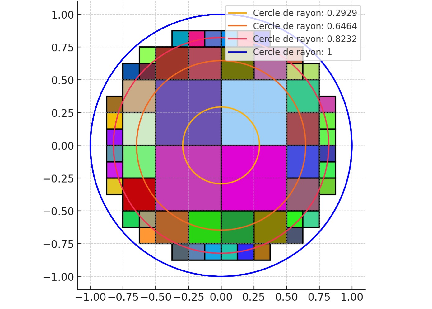
\includegraphics[width=7.249cm,height=5.193cm]{figures/Math_oraux-3.pdf}
  \caption{Carr{\'e}s dyadiques de tailles $1 / 8$, $1 / 4$, et $1 / 2$, ainsi
  que des disques de rayons $1 - \frac{\sqrt{2}}{2^n}$ pour $n = 1, 2, 3$ et
  le disque de rayon 1.}
\end{figure}


2- Soit $C = [- 1, 1]^2$ le carr{\'e} centr{\'e} {\`a} l'origine avec un
c{\^o}t{\'e} de longueur 2. Nous cherchons {\`a} montrer qu'il existe une
suite $\{D_i \}_{i \geq 0}$ de disques disjoints tels que :
\[ \sum_{i \geq 0} \text{Aire} (D_i) = 4. \]


Consid{\'e}rons le carr{\'e} $C$ moins un disque inscrit de rayon 1/2,
centr{\'e} {\`a} l'origine. L'aire de ce disque est donc $\frac{\pi}{4}$.

On commence d'abord par remarquer que tout carr{\'e} dyadique de taille $2^i$
partiellement ext{\'e}rieur {\`a} C ne peut partager une partie avec
l'int{\'e}rieur de C. En effet, empilons dans C $4$ carr{\'e}s dyadiques de
cot{\'e}s $1$.

Ainsi, si un carr{\'e} dyadique partage une partie avec l'int{\'e}rieur C, il
la partage forc{\'e}ment avec l'int{\'e}rieur de l'un de ces $4$ carr{\'e}s,
ce qui est absurde car les carr{\'e}s dyadiques ne peuvent pas se croiser
grace au lemme. \tmtextbf{}

De mani{\`e}re similaire {\`a} la premi{\`e}re partie du probl{\`e}me, la
r{\'e}gion restante dans le carr{\'e} $C$ peut {\^e}tre approxim{\'e}e aussi
pr{\'e}cis{\'e}ment que souhait{\'e} par un nombre fini de carr{\'e}s
dyadiques.

En effet, On va consid{\'e}rer une suite de disques de rayons $\frac{1}{2} +
\frac{\sqrt{2}}{2^{n + 1}}$ avec $n \geq 1$ (Pour qu'ils soient inclus dans le
carr{\'e}). Mais cette fois, on pave la r{\'e}gion entre chaque disque $D_n$
et le carr{\'e} par des carr{\'e}s dyadiques de cot{\'e}s ayant pour longueur
$1 / 2^{n + 1}$, comme pour la premi{\`e}re question, l'observation cl{\'e}
ici est que chaque carr{\'e} qui poss{\`e}de des points dans cette r{\'e}gion
est forc{\'e}ment {\`a} l'ext{\'e}rieur du disque de rayon $1 / 2$. (On pourra
s'en convaincre par in{\'e}galit{\'e} triangulaire).

On pourra ainsi construire une suite de carr{\'e}s dyadiques qui s'empilent
compl{\`e}tement dans la r{\'e}gion entre le carr{\'e} et le disque de rayon
$1 / 2$.

\begin{figure}[h]
  \centering
  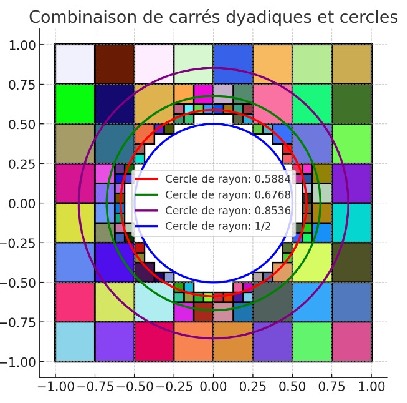
\includegraphics[width=6.831cm,height=6.761cm]{figures/Math_oraux-4.pdf}
  \caption{Carr{\'e}s dyadiques de tailles $1 / 16$, $1 / 8$, et $1 / 4$,
  ainsi que des disques de rayons $1 + \frac{\sqrt{2}}{2^{n + 1}}$ pour $n =
  1, 2, 3$ et le disque de rayon $1 / 2$ dans le carr{\'e} $[-1, 1]^2$.}
\end{figure}


\tmcolor{red}{}On construit la suite de disques par r{\'e}currence avec un
processus diagonal :

Pour $n = 1$, on place dans notre carr{\'e} les carr{\'e}s dyadiques de
cot{\'e} $\frac{1}{2^{n + 1}}$ avec $n = 1$, de fa{\c c}on {\`a} qu'ils ne
soient pas int{\'e}rieur du disque de rayon $\frac{1}{2} +
\frac{\sqrt{2}}{2^{n + 1}}$.

Ces carr{\'e}s sont en nombre fini et correspondent aux carr{\'e}s de niveau 1
pour le carr{\'e} $[- 1, 1]^2$(Voir la figure).

{\`A} l'int{\'e}rieur de ces carr{\'e}s, on place aussi par homoth{\'e}tie
des carr{\'e}s dyadiques de niveau 1 qui contiennent aussi un disque inscrit,
en gardant le m{\^e}me rapport homoth{\'e}tique.

Ces carr{\'e}s contiennent {\`a} leur tour d'autres carr{\'e}s de niveau 1
(c'est le processus diagonal qui permet de construire notre suite disjointe de
disques).

Ensuite, on inscrit des carr{\'e}s dyadiques de niveau 2 dans tous les
carr{\'e}s, et on consid{\`e}re une seconde couche de profondeur,
c'est-{\`a}-dire que dans les carr{\'e}s dyadiques inscrits dans les
carr{\'e}s dyadiques d{\'e}j{\`a} construits, on inscrit deux niveaux de
carr{\'e}s dyadiques suppl{\'e}mentaires, avec leurs disques associ{\'e}s.

On construit ainsi une suite disjointe de disques pour notre carr{\'e},
not{\'e} ($D'_n$).

Pour tout carr{\'e} $C$, on note $D'_n (C) = ((x_n (C), y_n (C), r_n (C)))$ la
suite des disques inscrits dans ce carr{\'e}, en r{\'e}alisant une
homoth{\'e}tie sur la suite construite dans le carr{\'e} $[- 1, 1]^2$.

Introduisons le rapport :
\[ A_C = \frac{\sum_{n = 1}^{\infty} \pi r_n^2 (C)}{\text{aire} (C)} \]


Soit $C$ le carr{\'e} utilis{\'e}. On remarque que $A_C$ ne d{\'e}pend pas du
choix du carr{\'e}, par homoth{\'e}tie. Notons le par $A$. L'aire totale
couverte par les disques est donn{\'e}e par :
\[ 4 A = \frac{\pi}{4} + A \sum_{i = 1}^{\infty} Aire (C_n) = \frac{\pi}{4} +
   \left( 4 - \frac{\pi}{4} \right) A, \]


o{\`u} $\frac{\pi}{4}$ est l'aire du disque inscrit, et $\left( 4 -
\frac{\pi}{4} \right) A$ est l'aire des disques ins{\'e}r{\'e}s dans la suite
des carr{\'e}s dyadiques $C_n$.

On trouve donc que $A = 1$.
\[ \maltese \maltese \maltese \maltese \maltese \maltese \maltese \]

Cet exercice, intitul{\'e} ``Certification de racines", propose un crit{\`e}re
pour garantir l'existence et l'unicit{\'e} d'un z{\'e}ro d'une fonction
diff{\'e}rentiable dans une boule donn{\'e}e. L'exercice fait appel {\`a} des
notions d'analyse et de topologie.
\begin{exercise}[(Certification de racines)]
Soit $f : \mathbb{R}^n \to \mathbb{R}^n$ une application de classe
$\mathcal{C}^1$. Soit $x \in \mathbb{R}^n$, soit $B$ la boule unit{\'e}
ferm{\'e}e. On suppose que pour tout $u, v \in B$,
\[ - f (x) + v - \mathrm{d} f (x + u) \cdot v \in \tfrac{1}{2} B. \]
Montrer que $f$ admet un unique z{\'e}ro dans la boule $x + B$.

\end{exercise}

\subsection*{Solution. (ZINE Akram)}
\addcontentsline{toc}{subsection}{Solution. (ZINE Akram)}


Soit $x \in B$, alors $\|f (x) - x\| \leq \frac{1}{2}$. En effet,
\[ f (x) = f (0) + \int_0^1 df_{tx} (x) \hspace{0.17em} dt = f (0) + \int_0^1
   (x - f (0) + h (t))  \hspace{0.17em} dt, \]


avec $\|h (t)\| \leq \frac{1}{2}$ pour tout $t \in [0, 1]$. Donc,
\[ \|f (x) - x\|= \left| \int_0^1 h (t) \hspace{0.17em} dt \right| \leq
   \int_0^1 \|h (t)\| \hspace{0.17em} dt \leq \frac{1}{2} . \]


Soit $g (x) =\|f (x)\|^2$ sur $B$. Comme $g$ est continue sur le compact $B$,
elle admet un minimum.

Avec $v = 0$, on a $\|f (0)\| \leq \frac{1}{2}$. Si $x \in \partial B$, alors
$\|f (x)\| \geq \frac{1}{2}$. Donc, le minimum de $g$ sur $B$ est au plus
$\frac{1}{4}$. Si le minimum est atteint en $0$, c'est fait, sinon il est
atteint {\`a} l'int{\'e}rieur de $B$.

Soit $a \in \overset{\circ}{B}$ un point o{\`u} $g$ atteint son minimum. Alors
$dg_a = 0$, c'est-{\`a}-dire pour tout \ $h \in \mathbb{R}^n, \langle df_a
(h), f (a) \rangle = 0$. Si $df_a$ est inversible, on en d{\'e}duit $f (a) =
0$.

Pour prouver que $df_a$ est injective, supposons le contraire. Alors, il
existe $w \in \ker (df_a)$, $\|w\|= 1$. On a aussi $df_a (- w) = 0$. Donc,
$\|w - f (0)\| \leq \frac{1}{2}$ et $\|- w - f (0)\| \leq \frac{1}{2}$, ce qui
est impossible, car $\|w - (- w)\|= 2$ alors que la sph{\`e}re $S (f (0),
\frac{1}{2})$ a un diam{\`e}tre de $1$.

Enfin, supposons qu'il existe $a, b \in B$ tels que $f (a) = f (b) = 0$ et $a
\neq b$. On a :
\[ 0 = \int_0^1 df_{(1 - t) a + tb} (b - a) \hspace{0.17em} dt =\|a - b\|
   \int_0^1 df_{(1 - t) a + tb} \left( \frac{b - a}{\|b - a\|} \right) 
   \hspace{0.17em} dt. \]


Or,
\[ df_{(1 - t) a + tb} \left( \frac{b - a}{\|b - a\|} \right) = \frac{b -
   a}{\|b - a\|} - f (0) + h (t), \]


avec $\|h (t)\| \leq \frac{1}{2}$. On obtient alors
\[ \frac{b - a}{\|b - a\|} = f (0) - \int_0^1 h (t) d t. \]


Puisque $\|f (0)\| \leq \frac{1}{2}$ et $\|h\| \leq \frac{1}{2}$, on a
{\'e}galit{\'e} dans l'in{\'e}galit{\'e} triangulaire :
\[ f (0) = - \int_0^1 h (t) d t = \frac{b - a}{2\|b - a\|} . \]


En proc{\'e}dant de mani{\`e}re similaire, on trouve $f (0) = \frac{a -
b}{2\|b - a\|}$, ce qui implique $a = b$, ce qui est une contradiction.
\[ \maltese \maltese \maltese \maltese \maltese \maltese \maltese \]

L'exercice 22 porte sur la m{\'e}diane de moyennes de variables
al{\'e}atoires. Il demande de prouver une borne de probabilit{\'e} sur
l'{\'e}cart entre cette m{\'e}diane et la moyenne th{\'e}orique. L'exercice
fait appel {\`a} des notions de probabilit{\'e}s et de statistiques.

\begin{exercise}[(M{\'e}diane de moyennes)]
Soient $n, m \geq 1$ des entiers et soient $X_{i, j}$, pour $1 \leq i \leq n$
et $1 \leq j \leq m$, des variables al{\'e}atoires discr{\`e}tes i.i.d. de
variance $\sigma^2$ et de moyenne~$\mu$. Pour~$1 \leq i \leq n$, soit $Y_i =
\frac{1}{m}  \sum_{j = 1}^m X_{i, j}$. Soit $Z$ une m{\'e}diane de l'ensemble
$\{ Y_1, \ldots, Y_n \}$.

Montrer que
\[ \mathbb{P} \left[ |Z - \mu | \leq \frac{2 \sigma}{\sqrt{m}} \right] \geq 1
   - \left( \frac{3}{4} \right)^{\frac{n}{2}} . \]

\end{exercise}

\subsection*{Solution. (ZINE Akram, SABIR Ilyass)}
\addcontentsline{toc}{subsection}{Solution. (ZINE Akram, SABIR Ilyass)}

Esp{\'e}rance et Variance :\tmtextbf{}
\[ E [Y_i] = \mu \quad \text{et} \quad \text{Var} (Y_i) = \frac{\sigma^2}{m} .
\]


Pour chaque $Y_i$, appliquons l'in{\'e}galit{\'e} de Chebyshev pour estimer la
probabilit{\'e} que $Y_i$ s'{\'e}carte de $\mu$ de plus de $\frac{2
\sigma}{\sqrt{m}}$ :
\[ P \left( |Y_i - \mu | > \frac{2 \sigma}{\sqrt{m}} \right) \leq
   \frac{\text{Var} (Y_i)}{\left( \frac{2 \sigma}{\sqrt{m}} \right)^2} =
   \frac{\sigma^2 / m}{4 \sigma^2 / m} = \frac{1}{4} . \]


Ainsi,
\[ P \left( |Y_i - \mu | \leq \frac{2 \sigma}{\sqrt{m}} \right) \geq
   \frac{3}{4} . \]


La m{\'e}diane $Z$ de l'ensemble $\{Y_1, Y_2, \ldots, Y_n \}$ sera dans
l'intervalle $\left[ \mu - \frac{2 \sigma}{\sqrt{m}}, \mu + \frac{2
\sigma}{\sqrt{m}} \right]$ si au moins la moiti{\'e} des $Y_i$ se trouvent
dans cet intervalle.

D{\'e}finissons $S$ comme le nombre de $Y_i$ satisfaisant $|Y_i - \mu | \leq
\frac{2 \sigma}{\sqrt{m}}$. Chaque $Y_i$ satisfait cette condition avec une
probabilit{\'e} $p \geq \frac{3}{4}$, ind{\'e}pendamment des autres. Ainsi,
$S$ suit une loi binomiale $\mathcal{B}(n, p)$ avec $p \geq \frac{3}{4}$.

Pour obtenir une borne sur $P \left( S > \frac{n}{2} \right)$, nous allons
consid{\'e}rer la probabilit{\'e} compl{\'e}mentaire $P \left( S \leq
\frac{n}{2} \right)$ et la majorer.

Pour tout $t > 0$, l'in{\'e}galit{\'e} de Markov donne :


\[ P (S \leq k) = P (e^{- tS} \geq e^{- tk}) \leq \frac{E [e^{- tS}]}{e^{-
   tk}} . \]


Ici, nous choisissons $k = \frac{n}{2}$.

Comme $S = \sum_{i = 1}^n I_i$, o{\`u} $I_i$ est l'indicateur que $Y_i$ est
dans l'intervalle, et les $I_i$ sont ind{\'e}pendants, nous avons :
\[ E [e^{- tS}] = \prod_{i = 1}^n E [e^{- tI_i}] = (pe^{- t} + (1 - p))^n . \]


Nous devons choisir $t$ pour minimiser la borne. Pour cela, posons :
\[ f (t) = (pe^{- t} + 1 - p) e^{t / 2} . \]


Calculons la d{\'e}riv{\'e}e de $f (t)$ :
\[ f' (t) = \frac{d}{dt}  [(pe^{- t} + 1 - p) e^{t / 2}] = e^{t / 2}  \left( -
   pe^{- t} + \frac{1}{2} (pe^{- t} + 1 - p) \right) . \]


Pour trouver le minimum, r{\'e}solvons $f' (t) = 0$, cela revient {\`a}
r{\'e}soudre l'{\'e}quation
\[ - pe^{- t} + \frac{1}{2} (pe^{- t} + 1 - p) = 0 \]


Par suite,


\[ - 2 pe^{- t} + pe^{- t} + 1 - p = 0 \]


Ainsi,
\[ pe^{- t} = 1 - p \]


Donc,
\[ t = - \ln \left( \frac{1 - p}{p} \right) \]


Substituons $t = - \ln \left( \frac{1 - p}{p} \right)$ dans $f (t)$ :
\begin{eqnarray*}
  f (t) & = & (pe^{- t} + 1 - p) e^{t / 2} \\
  & = & \left( p \cdot \frac{1 - p}{p} + 1 - p \right) \left( \frac{p}{1 - p}
  \right)^{1 / 2}\\
  & = & 2 (1 - p) \cdot \frac{p}{1 - p} = 2 (p (1 - p))^{\frac{1}{2}}
\end{eqnarray*}


Ainsi, on a :
\[ P \left( S \leq \frac{n}{2} \right) \leq (4 p (1 - p))^{n / 2} . \]


$p (1 - p)$ d{\'e}croit pour $p \geq \frac{1}{2}$

Pour $p = \frac{3}{4}$, calculons cette expression :
\[ 4 p (1 - p) = 4 \cdot \frac{3}{4} \cdot \frac{1}{4} = \frac{3}{4} . \]


Donc,
\[ P \left( S \leq \frac{n}{2} \right) \leq \left( \frac{3}{4} \right)^{n / 2}
   . \]


Par cons{\'e}quent,
\[ P \left( S \geq \frac{n}{2} \right) \geq P \left( S > \frac{n}{2} \right)
   \geq 1 - \left( \frac{3}{4} \right)^{n / 2} . \]


Nous obtenons la borne souhait{\'e}e :
\[ P \left( |Z - \mu | \leq \frac{2 \sigma}{\sqrt{m}} \right) \geq 1 - \left(
   \frac{3}{4} \right)^{n / 2} . \]
\[ \maltese \maltese \maltese \maltese \maltese \maltese \maltese \]

Cet exercice s'int{\'e}resse aux sous-espaces stables d'un espace vectoriel
norm{\'e} de dimension finie. Il demande de prouver l'existence d'un
suppl{\'e}mentaire stable pour le sous-espace des vecteurs invariants par deux
endomorphismes commutant avec leur commutateur. L'exercice fait appel {\`a}
des notions d'alg{\`e}bre lin{\'e}aire et de th{\'e}orie des groupes.

\begin{exercise}[(Sous-espace stable)]
Soit~$V$ un espace vectoriel norm{\'e} de dimension finie. On consid{\`e}re
deux endomorphismes de~$V$, not{\'e}s $h_1$ et~$h_2$, pr{\'e}servant la norme,
et tels que $h_1$ et $h_2$ commutent avec leur commutateur~$h_1 h_2 h_1^{- 1}
h_2^{- 1}$.

Montrer que le sous-espace des vecteurs invariants par~$h_1$ et $h_2$ admet
un suppl{\'e}mentaire {\'e}galement stable par $h_1$ et $h_2$.

\end{exercise}

\subsection*{Solution. (ZINE Akram)}
\addcontentsline{toc}{subsection}{Solution. (ZINE Akram)}

\tmtextbf{Lemme 1.}

Soit $u$ un endomorphisme isom{\'e}trique d'un espace vectoriel norm{\'e} de
dimension finie.

Notons Inv$(u)$ l'espace des vecteurs invariants par $u$ et $S (u)$ son
suppl{\'e}mentaire.

En notant, Inv$(u) = \ker (u - \text{Id})$ et $S (u) = \text{Im} (u -
\text{Id})$. Alors $V = \text{Inv} (u) \oplus S (u)$.

\tmtextbf{Preuve du lemme 1.}

oit $x \in \text{Inv} (u) \cap S (u)$. Alors, il existe $y \in V$ tel que $u
(y) = x + y$. Comme $x \in \text{Inv} (u)$, on a $u (x) = x$.

Soit $n$ un entier positif. En it{\'e}rant, on obtient $u^n (y) = nx + y$.

Puisque $u$ est une isom{\'e}trie, pour tout $k$, on a
\[ \|u^k (y)\|=\|y\| \]


On a donc
\[ \|y + nx\|=\|y\| \]


Or,
\[ \|nx\| \leq \|nx + y\|+\|y\| \leq 2\|y\| \]


En divisant par $n$ et en passant {\`a} la limite, on obtient $\|x\|= 0$,
donc $x = 0$.

\

On commence par le cas particulier o{\`u} $h_1$ et $h_2$ commutent.

D'apr{\`e}s le \tmtextbf{lemme 1}, $V$ est la somme directe Inv$(h_1) \oplus
S (h_1)$.

Inv$(h_1)$ est stable par $h_2$ car ces endomorphismes commutent.

Soit $h_2'$ l'endomorphisme induit sur Inv$(h_1)$.

Alors, d'apr{\`e}s le \tmtextbf{lemme 1.}, Inv$(h_1)$ est la somme directe
Inv$(h_2') \oplus S (h_2')$.

Or, Inv$(h_2') = \text{Inv} (h_1) \cap \text{Inv} (h_2)$.

Finalement, $V$ est la somme directe Inv$(h_1) \cap \text{Inv} (h_2) \oplus
(S (h_2') + S (h_1))$. Le sous-espace suppl{\'e}mentaire $S (h_2') + S (h_1)$
est stable par $h_1$ et $h_2$, d'o{\`u} le r{\'e}sultat.

\

Revenons {\`a} l'{\'e}nonc{\'e} g{\'e}n{\'e}ral. On suppose que $h_1$ et
$h_2$ commutent avec leur commutateur $[h_1, h_2]$. Utilisons le
\tmtextbf{lemme} :
\[ V = \text{Inv} ([h_1, h_2]) \oplus S ([h_1, h_2]) \]


Inv$([h_1, h_2])$ est stable par $h_1$ et $h_2$. Consid{\'e}rons les
endomorphismes induits $h_1'$ et $h_2'$. Puisqu'ils commutent {\'e}galement
avec $[h_1, h_2]$, ils commutent entre eux. On revient ainsi au cas
particulier pr{\'e}c{\'e}dent, qui nous fournit un suppl{\'e}mentaire $F$
stable par $h_1'$ et $h_2'$ tel que
\[ \text{Inv$([h_1, h_2]) = \text{Inv} (h_1') \cap \text{Inv} (h_2') + F =
   \text{Inv} (h_1) \cap \text{Inv} (h_2) + F$} \]


car, Inv$(h_1) \cap \text{Inv} (h_2) \subseteq \text{Inv} ([h_1, h_2])$.

Ainsi, $V = \text{Inv} (h_1) \cap \text{Inv} (h_2) + (F + S ([h_1, h_2]))$

Ce qui conclut la d{\'e}monstration.
\[ \maltese \maltese \maltese \maltese \maltese \maltese \maltese \]

Cet exercice porte sur le th{\'e}or{\`e}me d'Hermite-Kakeya. Il demande de
prouver une caract{\'e}risation des paires de polyn{\^o}mes qui s'entrelacent,
c'est-{\`a}-dire dont les racines r{\'e}elles sont simples et altern{\'e}es.
L'exercice fait appel {\`a} des notions de th{\'e}orie des polyn{\^o}mes et
d'analyse r{\'e}elle.
\begin{exercise}[(Th{\'e}or{\`e}me d'Hermite--Kakeya)]
Soient $P$ et $Q \in \mathbb{R} [X]$ des polyn{\^o}mes non constants. On dit
que~$P$ et~$Q$ {\tmem{s'entrelacent}} si:

(1)~leurs racines sont r{\'e}elles et simples,

(2)~ils n'ont pas de racines r{\'e}elles communes,

(3)~entre deux racines cons{\'e}cutives de $Q$ (resp.~$P$), il y a une et une
seule racine de~$P$ (resp.~$Q$).

Montrer que si pour tout~$(\lambda, \mu) \in \mathbb{R}^2 \setminus \{ (0, 0)
\}$, les racines de $\lambda P + \mu Q$ sont toutes r{\'e}elles et simples,
alors $P$ et $Q$ s'entrelacent.

Montrer la r{\'e}ciproque.
\end{exercise}

\subsection*{Solution. (ETTOUSY Badr, ZINE Akram)}
\addcontentsline{toc}{subsection}{Solution. (ETTOUSY Badr, ZINE Akram)}


\tmtextbf{M{\'e}thode 1 : (ETTOUSY Badr)}

Soit $P$ et $Q$ dans $\mathbb{R} [X]$.

On suppose que $\forall (\lambda, \mu) \in \mathbb{R}^2$, le polyn{\^o}me
$\lambda P (X) + \mu Q (X)$ a toutes ses racines r{\'e}elles et simples.
Montrons que les racines de $P$ et $Q$ sont intercal{\'e}es (c'est-{\`a}-dire,
entre deux racines de $P$ il existe une racine de $Q$ et r{\'e}ciproquement).

En utilisant les couples $(\lambda, \mu) = (1, 0)$ et $(\lambda, \mu) = (0,
1)$, on voit d{\'e}j{\`a} que $P$ et $Q$ doivent avoir toutes leurs racines
r{\'e}elles. Les polyn{\^o}mes $P$ et $Q$ jouant des r{\^o}les
sym{\'e}triques, il suffit de montrer qu'entre deux racines de $P$, il existe
au moins une racine de $Q$.

Soit $a$ et $b$ deux racines cons{\'e}cutives de $P$, et supposons que $Q$ ne
s'annule pas sur $[a, b]$. La fraction rationnelle $R (x) = \frac{P (x)}{Q
(x)}$ est donc de classe $C^1$ sur $[a, b]$ avec $R (a) = R (b) = 0$.

D'apr{\`e}s le th{\'e}or{\`e}me de Rolle, il existe $c \in] a, b [$ tel que
$R' (c) = 0$. La fraction rationnelle $R (x) - R (c)$ admet donc $c$ comme
z{\'e}ro de multiplicit{\'e} au moins 2.

En vertu du lemme suivant, pour $r$ assez petit, il existe sur la
circonf{\'e}rence $|z - c| = r$ au moins quatre points tels que Im$(R (z) - R
(c)) = 0$, soit Im$\hspace{0.17em} R (z) = 0$. L'un au moins de ces points
$z_0$ n'est pas r{\'e}el. Alors, $R (z_0) = \mu \in \mathbb{R}$. Le
polyn{\^o}me $P (x) - \mu Q (x)$ s'annule en un point $z_0$ non r{\'e}el, ce
qui contredit notre hypoth{\`e}se.

\tmtextbf{Lemme 1.}

Soit $R$ une fraction rationnelle qui admet $z_0$ comme racine de
multiplicit{\'e} $k$. Alors, pour $r$ assez petit, il existe au moins $2 k$
points v{\'e}rifiant $|z - z_0 | = r$ et Im$\hspace{0.17em} R (z) = 0$.

\tmtextbf{Preuve du lemme 1.}

Posons $z - z_0 = re^{i \theta}$ et $\frac{1}{k!} R^{(k)} (z_0) = \rho e^{i
\alpha}$.

La formule de Taylor Young nous dit alors que
\[ R (z) = \rho r^k e^{i (\alpha + k \theta)}  (1 + \varepsilon (z - z_0)) \]


avec $\underset{u \to 0}{\lim}  \varepsilon (u) = 0$. Soit $\eta > 0$ tel que
$|u| < \eta$ et $| \varepsilon (u) | < 1$, et choisissons $r < \eta$.

Posons $f (\theta) = \text{Im} \hspace{0.17em} R (z_0 + re^{i \theta})$,
$\varepsilon (u) = \varepsilon_1 (u) + i \varepsilon_2 (u)$, avec
$\varepsilon_1 (u)$ et $\varepsilon_2 (u)$ r{\'e}els. On obtient :
\[ f (\theta) = \text{Im} \hspace{0.17em} R (z) = \rho r^k  (\cos (\alpha + k
   \theta) \varepsilon_2 (z - z_0) + \sin (\alpha + k \theta) (1 +
   \varepsilon_2 (z - z_0))) \]


D{\'e}finissons $\theta_m$ pour $m \in \{0, 1, \ldots, 2 k\}$ par $\alpha + k
\theta_m = m \pi + \frac{\pi}{2}$. On a alors :
\[ f (\theta_m) = \rho r^k  (- 1)^m  (1 + \beta_m) \]
\

avec $| \beta_m | < 1$. Donc $f (\theta_m)$ est du signe de $(- 1)^m$. La
fonction $f$ change donc $2 k + 1$ fois de signe sur un intervalle de longueur
$2 \pi$, et donc elle s'annule au moins $2 k$ fois, ce qui ach{\`e}ve la
d{\'e}monstration.

\tmtextbf{La r{\'e}ciproque }

Soit $(P, Q)$ un couple de polyn{\^o}mes r{\'e}els simplement scind{\'e}s tels
qu'entre deux racines de l'un il y ait toujours au moins une racine de
l'autre. Montrons que le polyn{\^o}me $\lambda P + \mu Q$ reste scind{\'e}
lorsque le couple $(\lambda, \mu)$ d{\'e}crit $\mathbb{R}^2$.

Il est loisible de se ramener au cas o{\`u} $\lambda \neq 0$ et o{\`u} les
deux polyn{\^o}mes sont de la forme :
\[ P = \prod_{i = 1}^n (X - a_i) \infixand Q = \prod_{j = 1}^m (X - b_j) \]


avec $m = n$ ou $m = n - 1$. Nous supposerons de plus que :
\[ a_1 < b_1 < a_2 < b_2 < \ldots < a_n < b_n \tmop{si} m = n \]


cas que nous traiterons en premier.

Le signe des valeurs de la fonction rationnelle $P / Q$ aux voisinages des
infinis et des r{\'e}els $b_j$, ainsi que son annulation en les r{\'e}els
$a_i$, montre que l'{\'e}quation $\lambda P (x) + \mu Q (x) = 0$ poss{\`e}de
au moins $n$ racines r{\'e}elles si $\lambda + \mu \neq 0$, {\`a} savoir une
dans chaque intervalle $] b_j, b_{j + 1} [$ et une autre dans l'un des deux
intervalles $] - \infty, b_1 [$ et $] b_n, + \infty [$, et au moins $n - 1$
racines r{\'e}elles dans le cas contraire -- la derni{\`e}re pouvant {\^e}tre
alors consid{\'e}r{\'e}e comme {\'e}tant devenue infinie.

Ce nombre de racines {\'e}tant toujours exactement {\'e}gal au degr{\'e} de
$\lambda P + \mu Q$, ce dernier polyn{\^o}me est donc (simplement) scind{\'e}.

Il en va tout de m{\^e}me si $m = n - 1$ (ici d'ailleurs le degr{\'e} de
$\lambda P + \mu Q$ est toujours {\'e}gal {\`a} $n$). Enfin $\lambda P + \mu
Q$ est scind{\'e} (mais alors non simplement) dans le cas $\lambda = \mu = 0$.

\tmtextbf{M{\'e}thode 2 : (ZINE Akram)}

Raisonnons par contrapos{\'e}e. Supposons que $P$ et $Q$ ne s'entrelacent pas.
Cela signifie qu'il existe deux racines $\lambda_1$ et $\lambda_2$ de $P$
telles qu'il n'y ait aucune racine de $Q$ entre elles. D{\'e}finissons alors
la fonction $F = \frac{P}{Q}$. Puisque $Q$ n'a pas de racine entre $\lambda_1$
et $\lambda_2$, $F$ est bien d{\'e}finie sur cet intervalle. De plus, nous
avons $F (\lambda_1) = F (\lambda_2) = 0$.

D'apr{\`e}s le th{\'e}or{\`e}me de Rolle, il existe un point $c$ situ{\'e}
entre $\lambda_1$ et $\lambda_2$ tel que $F' (c) = 0$.

Calculons alors $F' (x) = \left( \frac{P}{Q} \right)'$. En utilisant la
formule de d{\'e}rivation du quotient, on obtient :
\[ F' (x) = \frac{P' (x) Q (x) - P (x) Q' (x)}{Q (x)^2} . \]


Comme $F' (c) = 0$, cela implique que $P' (c) Q (c) - P (c) Q' (c) = 0$.
Puisque $Q (c) \neq 0$ (car $Q$ n'a pas de racine entre $\lambda_1$ et
$\lambda_2$), nous en d{\'e}duisons que $P (c) Q' (c) = P' (c) Q (c$).

Consid{\'e}rons alors le polyn{\^o}me $T = P + \alpha Q$, o{\`u} $\alpha = - F
(c)$. Puisque $F' (c) = 0$, $c$est une racine double de $T$. Ceci contredit
l'hypoth{\`e}se que pour tout $(\lambda, \mu) \in \mathbb{R}^2 \setminus \{(0,
0)\}$, les racines de $\lambda P + \mu Q$ sont toutes r{\'e}elles et simples.
Ainsi, nous avons montr{\'e} par contrapos{\'e}e que $P$ et $Q$ doivent
s'entrelacer.

\tmtextbf{Preuve du sens inverse}

Supposons maintenant que $P$ et $Q$ s'entrelacent. Nous voulons montrer que
pour tout $(\lambda, \mu) \in \mathbb{R}^2 \setminus \{(0, 0)\}$, les racines
de $R = \lambda P + \mu Q$ sont toutes r{\'e}elles et simples. Supposons que
$\lambda$ et $\mu$ sont non nuls ; sinon, la conclusion est triviale.

Soit $n = \deg P$ et $m = \deg Q$.

On suppose, sans perte de g{\'e}n{\'e}ralit{\'e}, que $n \geq m$ et que $p_1 <
q_1$.

Traitons le cas $n > m$ : \tmcolor{red}{}

On a alors $m = n - 1$. Pour tout $i \leq n - 1$, $R (p_i) = \mu Q (p_i)$ et
$R (p_{i + 1}) = \mu Q (p_{i + 1})$. Comme $Q$ change de signe en $q_i$, $R$
change {\'e}galement de signe sur $[p_i, p_{i + 1}]$ et admet donc une racine
sur cet intervalle. Ceci {\'e}tant vrai pour tout $i$, $R$ admet $n - 1$
racines r{\'e}elles distinctes.

Si $n$ est pair, soit $p$ et $q$ les coefficients dominants de $P$ et $Q$
respectivement. On a $\frac{R}{\mu q} (p_1) < 0$ et $\underset{x \to -
\infty}{\lim }  \frac{R}{\lambda p} (x) > 0$ ainsi que $\frac{R}{\mu q} (p_n)
> 0$ et $\underset{x \to \infty}{\lim }  \frac{R}{\lambda p} (x) > 0$. Par
cons{\'e}quent, l'un des deux couples $(\underset{x \to - \infty}{\lim } R
(x), R (p_1))$ ou $(R (p_n), \underset{x \to \infty}{\lim } R (x))$
poss{\`e}de deux {\'e}l{\'e}ments de signes oppos{\'e}s. Le th{\'e}or{\`e}me
des valeurs interm{\'e}diaires implique alors l'existence d'une
$n^{\text{i{\`e}me}}$ racine.

Si $n$ est impair, la conclusion reste la m{\^e}me.

Ainsi, $R$ poss{\`e}de $n$ racines r{\'e}elles distinctes et son degr{\'e} est
$n$, d'o{\`u} le r{\'e}sultat.

Le cas $n = m$ se traite de la m{\^e}me fa{\c c}on en prouvant que $n - 1$
racines de $R$ se trouvent dans les intervalles $[q_i, q_{i + 1}]$. Pour la
racine restante, on raisonne sur les couples $(\underset{x \to - \infty}{\lim}
R (x), R (q_1))$ et $(R (q_n), \underset{x \to \infty}{\lim}  R (x))$.
\[ \maltese \maltese \maltese \maltese \maltese \maltese \maltese \]

L'exercice 25 s'int{\'e}resse {\`a} un groupe particulier de polyn{\^o}mes. Il
demande de d{\'e}crire le groupe des {\'e}l{\'e}ments inversibles dans un
certain anneau de fractions rationnelles {\`a} coefficients dans $\mathbb{Z}/
p^2 \mathbb{Z}$, et de prouver que ce groupe n'est pas finiment engendr{\'e}.
L'exercice fait appel {\`a} des notions d'alg{\`e}bre et de th{\'e}orie des
groupes.
\begin{exercise}[(Un groupe de polyn{\^o}mes)]
Soit~$p$ un nombre premier. On consid{\`e}re l'anneau $A$ des fractions
rationnelles en $X$ {\`a} coefficients dans $\mathbb{Z}/ p^2 \mathbb{Z}$ de la
forme~$X^{- k} P (X)$, avec~$P$ un polyn{\^o}me. D{\'e}crire le groupe
$A^{\times}$ des {\'e}l{\'e}ments inversibles (pour la multiplication) et
montrer qu'il n'est pas engendr{\'e} par un nombre fini d'{\'e}l{\'e}ments.

\end{exercise}

\subsection*{Solution. (ZINE Akram)}
\addcontentsline{toc}{subsection}{Solution. (ZINE Akram)}


\tmtextbf{Lemme 1.}

Soit $G = \langle g_1, g_2, \ldots, g_n \rangle$ un groupe ab{\'e}lien
finiment engendr{\'e} et soit $N$ un sous-groupe de $G$. Alors, $N$ est
{\'e}galement finiment engendr{\'e}.

\tmtextbf{Preuve du lemme 1.}

Nous proc{\'e}dons par r{\'e}currence sur le nombre $n$ de g{\'e}n{\'e}rateurs
de $G$.

Le cas de base est trivial cas tout sous groupe d'un groupe cyclique est
cyclique.

Supposons maintenant que le lemme est vrai pour tout groupe ab{\'e}lien
finiment engendr{\'e} avec $n - 1$ g{\'e}n{\'e}rateurs.

Soit $G = \langle g_1, g_2, \ldots, g_n \rangle$ et soit $N$ un sous-groupe
de $G$. Consid{\'e}rons le sous-groupe
\[ M = N \cap \langle g_2, \ldots, g_n \rangle . \]


Ce sous-groupe $M$ est un sous-groupe de $\langle g_2, \ldots, g_n \rangle$,
qui est un groupe ab{\'e}lien finiment engendr{\'e} avec $n - 1$
g{\'e}n{\'e}rateurs.

Par hypoth{\`e}se de r{\'e}currence, $M$ est donc finiment engendr{\'e}.

Soit $M = \langle x_1, x_2, \ldots, x_m \rangle$ avec $x_i \in M$. Ensuite,
consid{\'e}rons les {\'e}l{\'e}ments de $N$ qui impliquent $g_1$.
D{\'e}finissons l'ensemble
\[ A =\{a \in \mathbb{Z} \mid \exists b_2, \ldots, b_n \in \mathbb{Z}
   \text{tels que } g_1^a g_2^{b_2} \ldots g_n^{b_n} \in N\}. \]


Cet ensemble $A$ est un sous-groupe de $\mathbb{Z}$, et tout sous-groupe de
$\mathbb{Z}$ est de la forme $d\mathbb{Z}$ pour un certain entier $d$.

Par cons{\'e}quent, il existe un entier $d$ tel que $A = d\mathbb{Z}$. Cela
signifie qu'il existe des entiers $b_2, \ldots, b_n$ tels que
\[ x = g_1^d g_2^{b_2} \ldots g_n^{b_n} \in N. \]


Nous affirmons maintenant que $N = \langle x_1, \ldots, x_m, x \rangle$.
Prenons un {\'e}l{\'e}ment quelconque $g \in N$. Comme $g \in G$, il peut
s'{\'e}crire sous la forme
\[ g = g_1^{c_1} g_2^{c_2} \ldots g_n^{D_n} . \]


Par la d{\'e}finition de $A$, nous avons $c_1 \in A = d\mathbb{Z}$, donc il
existe un entier $h$ tel que $c_1 = dh$. Consid{\'e}rons alors
\[ gx^{- h} = g_1^{c_1 - dh} g_2^{c_2} \ldots g_n^{D_n} = g_2^{c_2} \ldots
   g_n^{D_n} . \]


Cet {\'e}l{\'e}ment appartient {\`a} $M$, qui est engendr{\'e} par $x_1,
\ldots, x_m$. Ainsi, nous avons
\[ g = x^h (x_1^{e_1} x_2^{e_2} \ldots x_m^{e_m}), \]


o{\`u} $e_i \in \mathbb{Z}$. Cela montre que chaque {\'e}l{\'e}ment de $N$
peut {\^e}tre {\'e}crit comme une combinaison des {\'e}l{\'e}ments $x_1,
\ldots, x_m, x$.

Par cons{\'e}quent, $N$ est finiment engendr{\'e}, ce qui conclut la preuve du
lemme.

\

Revenons {\`a} l'exercice.

\

Pour caract{\'e}riser les {\'e}l{\'e}ments inversibles de $A$, nous devons
montrer que $X^{- k} P (X)$ est inversible si et seulement si $P$ a exactement
un coefficient non divisible par $p$. Supposons que $X^{- k} P (X)$ soit
inversible : il existe alors un polyn{\^o}me $Q (X)$ et un entier natuel $l$
tels que
\[ (X^{- k} P (X)) (X^{- l} Q (X)) = 1_A . \]


Cela implique que tous les coefficients de $PQ - X^{k + l}$ sont des multiples
de $p^2$. En r{\'e}duisant modulo $p$, on trouve que $PQ = X^{k + l}$ dans
$\mathbb{F}_p [X]$. Comme $\mathbb{F}_p$ est un corps et que $X$ est
irr{\'e}ductible dans $\mathbb{F}_p [X]$, cela signifie que $P = \alpha X^i$
pour un certain $\alpha \in \mathbb{F}_p \setminus \{0\}$. Ainsi, $P$
poss{\`e}de exactement un coefficient non divisible par $p$.

R{\'e}ciproquement, supposons que $P = \alpha X^i + pQ (X)$ avec $\alpha$ non
divisible par $p$.

Soit $b$ l'inverse de $a$ modulo $p^2$. On trouve modulo $p^2$ que $P (X) =
aX^i (1 + pbX^{- i} Q (X))$ En posant $y = bX^{k - i} (1 - pbX^{- i} Q (X))$.
On trouve que $(X^{- k} P (X)) y = 1_A$, prouvant que $X^{- k} P (X)$ est
inversible.

Consid{\'e}rons maintenant le sous-groupe S de $A^{\times}$.
\[ S = \left\{ \alpha + pQ (X) \mid \alpha \in \mathbb{Z}, \hspace{0.17em}
   \alpha \neq 0 \pmod{p}, \hspace{0.17em} Q (X) \in \mathbb{Z}[X] \right\} \]


Consid{\'e}rons maintenant que le sous-groupe $S$ est g{\'e}n{\'e}r{\'e} par
un ensemble fini d'{\'e}l{\'e}ments $s_1, s_2, \ldots, s_n$, o{\`u} chaque
$s_i$ est de la forme :
\[ s_i = \alpha_i + pQ_i (X) \]


avec $\alpha_i \in \mathbb{Z}$, $\alpha_i \neq 0 \pmod{p}$, et $Q_i (X) \in
\mathbb{Z}[X]$. On suppose que ces $s_i$ forment un syst{\`e}me de
g{\'e}n{\'e}rateurs de $S$.

Cependant, une contradiction {\'e}merge lorsque l'on examine le produit de
deux g{\'e}n{\'e}rateurs $s_i$ et $s_j$. Prenons deux {\'e}l{\'e}ments $s_i =
\alpha_i + pQ_i (X)$ et $s_j = \alpha_j + pQ_j (X)$ dans $S$, et
consid{\'e}rons leur produit :
\[ s_i s_j = (\alpha_i + pQ_i (X)) (\alpha_j + pQ_j (X)) = \alpha_i \alpha_j +
   p (\alpha_i Q_j (X) + \alpha_j Q_i (X)) + p^2 Q_i (X) Q_j (X) \]


Le terme $p^2 Q_i (X) Q_j (X)$ dispara{\^i}t dans l'anneau $\mathbb{Z}/ p^2
\mathbb{Z}$. Ainsi, le produit devient :
\[ s_i s_j = \alpha_i \alpha_j + p (\alpha_i Q_j (X) + \alpha_j Q_i (X)) \]


Le degr{\'e} du polyn{\^o}me reste born{\'e} par $M = \max (\deg Q_i)_{1 \leq
i \leq n}$. Ceci est valable pour un produit aussi long que l'on souhaite.

En consid{\'e}rant le polyn{\^o}me $1 + pQ^{M + 1} (X)$. Il est dans S mais ne
peut {\^e}tre g{\'e}n{\'e}r{\'e} par un produit des g{\'e}n{\'e}rateurs de S.
Et cela est une contradiction.
\[ \maltese \maltese \maltese \maltese \maltese \maltese \maltese \]

Cet exercice comporte deux parties distinctes. La premi{\`e}re traite des
matrices de trace nulle dans $\mathrm{SL}_2 (\mathbb{Z})$, demandant de
prouver une propri{\'e}t{\'e} de conjugaison. La seconde partie concerne les
sommes de deux carr{\'e}s, demandant de prouver une condition suffisante pour
qu'un entier soit la somme de deux carr{\'e}s. L'exercice fait appel {\`a} des
notions d'alg{\`e}bre lin{\'e}aire et de th{\'e}orie des nombres.

\begin{exercise}[(Matrices de traces nulles et sommes de deux
carr{\'e}s)]
Soient~$A, B \in \mathrm{SL}_2 (\mathbb{Z})$ (le groupe des matrices $2 \times
2$ {\`a} coefficients entiers et d{\'e}terminant~1).

1. Montrer que si~$\mathrm{Tr} (A) = \mathrm{Tr} (B) = 0$, alors~$A$ est
conjugu{\'e}e {\`a}~$B$ ou~$- B$.

2. Montrer que si~$n > 1$ et~$x$ sont des entiers tels que~$x^2 \equiv - 1
\pmod{n}$, alors il existe des entiers~$a$ et~$b$ tels que~$n = a^2 + b^2$.

\end{exercise}

\subsection*{Solution. (ETTOUSY Badr - ZINE Akram)}
\addcontentsline{toc}{subsection}{Solution. (ETTOUSY Badr - ZINE Akram)}


\tmtextbf{1.} Consid{\'e}rons $x, y, a, b, c, d \in \mathbb{Z}$, \ et
d{\'e}finissons $\alpha_{x, y} \assign \left(\begin{array}{c}
  x\\
  y
\end{array}\right) \in \mathbb{Z}^2$, et $A \assign \left(\begin{array}{cc}
  a & c\\
  b & d
\end{array}\right) \in \tmop{SL}_2 (\mathbb{Z})$.

Supposons que $b > 0$. On consid{\`e}re $M_{x, y} = (\alpha, A \alpha)$ et on
souhaite d{\'e}montrer que :
\[ \det M_{x, y} bx^2 + (d - a) xy - cy^2 = 1 \]


En utilisant la compl{\'e}tion du carr{\'e} et par le fait que $a + d = 0$ et
$a^2 + bc = - 1$, que :
\[ \det M_{x, y} = \frac{(bx - ay)^2 + y^2}{b} \]


Ainsi, $\det M_{x, y} > 0$ pour tout $(x, y) \in \mathbb{Z}^2 \setminus \{(0,
0)\}$.

\tmtextbf{D{\'e}termination de $e$}

D{\'e}finissons $e = \underset{(x, y) \in \mathbb{Z}^2 \setminus \{(0,
0)\}}{\inf} \det M_{x, y}$. Nous allons prouver le lemme suivant :

\

\tmtextbf{Lemme 1.}

$e = \underset{(x, y) \in \mathbb{Z}^2 \setminus \{(0, 0)\}}{\inf} \det M_{x,
y}$ est atteint et on a $3 e^2 \leq - 4 (bc + a^2)$.

\tmtextbf{Preuve du lemme 1.}

\

Notons $m = \underset{(x, y) \in \mathbb{R}^2 \setminus \{(0, 0)\}}{\inf}
\det M_{x, y}$. Il est atteint car le cercle unit{\'e} de $\mathbb{R}^2$ est
compact. Par homog{\'e}n{\'e}it{\'e} de la forme quadratique, on a
\[ \det M_{x, y} \geq m (x^2 + y^2) \]


Soit $N$ un entier naturel tel que $N \geq \sqrt{\frac{e + 1}{m}}$.
D'apr{\`e}s ce qui pr{\'e}c{\`e}de, si $(x, y) \in \mathbb{Z}^2$ et $\lvert x
\rvert > N$ ou $\lvert y \rvert > N$, alors $\det M_{x, y} \geq e + 1$.

Donc, $e = \underset{\lvert x \rvert \leq N, \lvert y \rvert \leq
N}{\underset{(x, y) \in \mathbb{Z}^2 \setminus \{(0, 0)\}}{\inf}}  \det M_{x,
y}$ est atteint car l'ensemble est fini.

Soit $(\alpha, \beta) \in \mathbb{Z}^2$ tel que $\tmop{detM}_{\alpha, \beta} =
e$. Notons $d = \tmop{pgcd} (\alpha, \beta)$ et $\alpha'$, $\beta'$ les
entiers tels que $\alpha = d \alpha'$ et $\beta = d \beta'$. On obtient
\[ e = d^2 q (\alpha', \beta') \geq d^2 e \]


Ainsi, $d = 1$. D'apr{\`e}s le th{\'e}or{\`e}me de B{\'e}zout, il existe
$(\gamma, \delta)$ tel que $\alpha \delta + \beta \delta = 1$. Posons $v = (-
\delta, \gamma)$.

$P = \left(\begin{array}{cc}
  \alpha & - \delta\\
  \beta & \gamma
\end{array}\right)$ et $P^{- 1}$ est la matrice de passage de $(u, v)$ {\`a}
$(e_1, e_2)$ (base canonique de $\mathbb{R}^2$). Donc, $\mathbb{Z}^2
=\mathbb{Z}u +\mathbb{Z}v$.

Il existe $(a', c')$ tels que, dans la base $(u, v)$ on ait $q (x, y) = ex^2 +
2 a' xy + c' y^2$. On a :
\[ \left(\begin{array}{cc}
     e & a'\\
     a' & c'
   \end{array}\right) = P^{\top} \left(\begin{array}{cc}
     b & - a\\
     - a & - c
   \end{array}\right) P \]


et donc $c' {e - a'}^2 = (\det P)^2  (- bc - a^2) = - bc - a^2$.

Pour tout $(x, y) \in \mathbb{Z}^2$, on obtient
\[ q (xu + yv) = e \left( x + \frac{a'}{e} y \right)^2 + \left( c' -
   \frac{(a')^2}{e} \right) y^2 \]


En prenant $y = 1$ et en choisissant $n \in \mathbb{Z}$ tel que $\lvert n +
\frac{a'}{e} \rvert \leq \frac{1}{2}$, on a
\[ e \leq q (nu + v) \leq \frac{e}{4} + c' - \frac{(a')^2}{e} \]


et donc $3 e^2 \leq - 4 (bc + a^2)$.

\tmtextbf{Conclusion.}

Ainsi, comme $e > 0$, on a $e = 1$. D'o{\`u} il existe $\alpha \in \mathbb{R}$
tel que $\det M = 1$.

La matrice $A$ dans la base $(\alpha, A \alpha)$ est sous la forme :
\[ \left(\begin{array}{cc}
     0 & m\\
     1 & n
   \end{array}\right) \]
avec $m, n \in \mathbb{Z}$. Le d{\'e}terminant et la trace sont conserv{\'e}s
par conjugaison. Ainsi, on trouve que $n = 0$ et $m = - 1$.

Si $b < 0$, on consid{\`e}re la base $(A \alpha, \alpha)$. Dans ce cas, $- b
> 0$ et on introduit une forme quadratique de la m{\^e}me fa{\c c}on (avec
pour coefficient dominant $- b$). On obtient ainsi que $A$ est conjugu{\'e}e
{\`a} $\left(\begin{array}{cc}
  0 & 1\\
  - 1 & 0
\end{array}\right)$ ou $\left(\begin{array}{cc}
  0 & - 1\\
  1 & 0
\end{array}\right)$.

Cela implique que pour toute matrice $B$ sans SL$_2 (\mathbb{Z})$ telle que
$\det B = 1$ et Tr$(B) = 0$, $A$ est conjugu{\'e}e {\`a} $B$ ou $- B$.

\tmtextbf{2.} Si a et b sont somme de carr{\'e}s $a = x^2 + y^2$ et $b = z^2 +
t^2$ alors $ab = (xz - yt)^2 + (xt + yz)^2$ On va se r{\'e}duire donc au cas
o{\`u} n est premier.

\

\tmtextbf{Lemme 2.}

Soit $p$ premier. Pour tout $a \in \mathbb{Z}$, $p \nmid a$. Il existe $x, y
\in \{1, 2, \ldots, \lfloor \sqrt{p} \rfloor\}$ tels que $ax \equiv y
\pmod{p}$ ou $ax \equiv - y \pmod{p}$.

\

\tmtextbf{Preuve du lemme 2.}

Consid{\'e}rons $S = \{1, 2, \ldots, \lfloor \sqrt{p} \rfloor\}^2$. On a $p <
(\lfloor \sqrt{p} \rfloor + 1)^2$, et donc card$(S) > p$. D'apr{\`e}s le
principe des tiroirs, il existe $(x_1, y_1) \neq (x_2, y_2)$ telles que $ax_1
- y_1 \equiv ax_2 - y_2 \pmod{p}$. On prouve facilement par l'absurde que $x$
et $y$ sont non nuls. D'o{\`u} le r{\'e}sultat.

\

\tmtextbf{Conclusion.}

Revenons {\`a} notre question, soit $x \in \mathbb{Z}$ tel que $x^2 \equiv - 1
\pmod{p}$. On a $p \nmid x$. Il existe $a, b$ d'apr{\`e}s le lemme tels que
$xa \equiv \pm b \pmod{p}$. On a $x^2 a^2 + a^2 = b^2 + a^2 \equiv 0
\pmod{p}$, et donc $a^2 + b^2 = kp$ avec $k \in \mathbb{Z}$. On a $x^2 + y^2
\geq 2$. Ainsi $k > 0$.

Nous montrons que $k = 1$. $a, b \leq \lfloor \sqrt{p} \rfloor$, d'o{\`u}
$a^2 + b^2 < 2 p$. Or, $p / a^2 + b^2$, d'o{\`u} $p = a^2 + b^2$.
\[ \maltese \maltese \maltese \maltese \maltese \maltese \maltese \]

L'exercice 27 porte sur le th{\'e}or{\`e}me d'Hermite-Sylvester. Il demande
d'{\'e}tudier les propri{\'e}t{\'e}s d'une matrice construite {\`a} partir des
racines d'un polyn{\^o}me, notamment son rang et sa positivit{\'e}. L'exercice
fait appel {\`a} des notions d'alg{\`e}bre lin{\'e}aire et de th{\'e}orie des
polyn{\^o}mes.
\begin{exercise}[(Th{\'e}or{\`e}me d'Hermite-Sylvester)]
Soit~$P \in \mathbb{R} [X]$ un polyn{\^o}me de degr{\'e}~$n \geq 1$.
Soit~$\lambda_1, \ldots, \lambda_n \in \mathbb{C}$ ses racines, avec
multiplicit{\'e}. Soit~$H \in \mathbb{C}^{n \times n}$ la matrice d{\'e}finie
par
\[ H_{i, j} = \sum_{k = 1}^n \lambda_k^{i + j} . \]
Montrer que~$H$ est une matrice sym{\'e}trique r{\'e}elle. Montrer que le rang
de~$H$ est {\'e}gal au nombre de racines distincte, et que~$H$ est positive si
et seulement si toutes les racines sont r{\'e}elles.

\end{exercise}

\subsection*{Solution. (SABIR Ilyass)}
\addcontentsline{toc}{subsection}{Solution. (SABIR Ilyass)}

Soit $P \in \mathbb{R} [X]$ de degr{\'e} $n \geqslant 1$. Soient $\lambda_1,
\ldots, \lambda_n \in \mathbb{C}$ ses racines, avec multiplicit{\'e}.

Montrons que la matrice $H$ est une matrice r{\'e}elle sym{\'e}trique,

Pour tout $i, j \in \llbracket 1, n \rrbracket$, il est clair que \ $H_{i, j}
= H_{j, i}$. Donc $H$ est une matrice sym{\'e}trique.

\

Notons $\alpha_1, \ldots, \alpha_r \in \mathbb{R}$ et $\beta_1,
\overline{\beta_1}, \ldots, \beta_s, \overline{\beta_s} \in \mathbb{C}
\backslash \mathbb{R}$ les racines de $P$, et notons pour tout $i \in
\llbracket 1, r \rrbracket$ et pour tout $j \in \llbracket 1, s \rrbracket$
$\zeta_i$ l'ordre de multiplicit{\'e} de $\alpha_i$ et $\rho_j$ l'ordre de
multiplicit{\'e} de $\beta_j$ et de $\overline{{\beta_j} }$.

On a alors, pour tout $i, j \in \llbracket 1, n \rrbracket$
\begin{eqnarray*}
  H_{i, j} & = & \sum_{k = 1}^r {\zeta_k}  \lambda_k^{i + j} + \sum_{k = 1}^s
  \rho_k (\beta_k^{i + j} + \overline{{\beta_k}  }^{i + j})\\
  & = & \sum_{k = 1}^r {\zeta_k}  \lambda_k^{i + j} + 2 \sum_{k = 1}^s \rho_k
  \tmop{Re} (\beta_k^{i + j})\\
  & \in & \mathbb{R}
\end{eqnarray*}


Donc $H$ est une matrice r{\'e}elle. Montrons que le rang de~$H$ est {\'e}gal
au nombre de racines distincts.

\

Tout d'abord, observons que chaque racine $\lambda_k$ (compt{\'e}e avec
multiplicit{\'e}) d{\'e}finit un vecteur $v_k \in \mathbb{C}^n$ dont les
composantes sont :
\[ v_k = \left(\begin{array}{c}
     \lambda_k^1\\
     \lambda_k^2\\
     \vdots\\
     \lambda_k^n
   \end{array}\right) \]
Alors, $H$ peut s'exprimer comme :
\[ H = \sum_{k = 1}^n v_k v_k^T \]


\

Comme $P$ peut avoir des racines multiples, on peut regrouper les vecteurs
correspondant aux racines identiques.

\

Soient $\lambda^{(1)}, \ldots, \lambda^{(m)}$ les racines distinctes de $P$,
avec des multiplicit{\'e}s $n_1, \ldots, n_m$ (donc $\sum_{i = 1}^m n_i = n$).
D{\'e}finissons :
\[ w_i = \left(\begin{array}{c}
     (\lambda^{(i)})^1\\
     (\lambda^{(i)})^2\\
     \vdots\\
     (\lambda^{(i)})^n
   \end{array}\right) \]


Alors, $H$ devient :
\[ H = \sum_{i = 1}^m n_i w_i w_i^T \]


Comme chaque $w_i w_i^T$ est une matrice de rang $1$, et que les $w_i$
correspondant aux racines distinctes sont lin{\'e}airement ind{\'e}pendants
(car des racines distinctes donnent des vecteurs de puissances
lin{\'e}airement ind{\'e}pendants), le rang de $H$ est {\'e}gal au nombre de
racines distinctes :
\[ \mathrm{rang} (H) = m \]


o{\`u} $m$ est le nombre de racines distinctes de $P$.

\

Pour tout vecteur $x \in \mathbb{R}^n$, on a :
\[ x^T Hx = \sum_{k = 1}^n (x^T v_k)^2 \geq 0 \]


Cela montre que $H$ est semi-d{\'e}finie positive.
\begin{itemize}
  \item \tmtextbf{Si toutes les racines sont r{\'e}elles :}
  
  Les vecteurs $w_i$ sont r{\'e}els et lin{\'e}airement ind{\'e}pendants, donc
  $H$ est d{\'e}finie positive :
  \[ x^T Hx > 0 \quad \text{pour tout } x \in \mathbb{R}^n \setminus \{0\} \]
  \item \tmtextbf{S'il y a des racines complexes :}
  
  Les racines complexes apparaissent en paires conjugu{\'e}es $\lambda,
  \bar{\lambda}$. Les vecteurs correspondants $v_{\lambda}$ et
  $v_{\bar{\lambda}}$ v{\'e}rifient :
  \[ v_{\bar{\lambda}} = \overline{v_{\lambda}} \]
  La contribution {\`a} $H$ d'une paire de conjugu{\'e}s complexes est :
  \[ v_{\lambda} v_{\lambda}^T + v_{\bar{\lambda}} v_{\bar{\lambda}}^T \]
  Cette somme est r{\'e}elle et sym{\'e}trique, mais introduit une
  d{\'e}pendance lin{\'e}aire, ce qui fait que $H$ est seulement
  semi-d{\'e}finie positive. Sp{\'e}cifiquement, il existe des vecteurs non
  nuls $x$ tels que $x^T Hx = 0$, indiquant que $H$ n'est pas d{\'e}finie
  positive.
\end{itemize}


\tmtextbf{Commentaire.}

Pour montrer que $H$ est r{\'e}elle, on peut utiliser aussi le r{\'e}sultat
classique des formules de Newton :

\

\tmtextbf{Lemme 1. (Formules de Newton)}

Soit $N \geqslant 2$ un entier, et $K$ un corps commutatif, $x_1, \ldots, x_N$
des {\'e}l{\'e}ments de $K$. On consid{\`e}re, pour tout $p \in \mathbb{N}$ :
\[ S_p (x_1, \ldots, x_N) \assign \underset{i = 1}{\overset{N}{\sum}} x^p_i \]


\

On note $\sigma_1, \ldots, \sigma_N$ les fonctions sym{\'e}triques
{\'e}l{\'e}mentaires de $x_1, \ldots, x_N$ d{\'e}finies par :
\[ \sigma_k (x_1, \ldots, x_N) = \overset{}{\underset{1 \leqslant j_1 < \cdots
   < j_k \leqslant N}{\sum}}  \underset{l = 1}{\overset{k}{\prod}} x_{j_l},
   \forall k = 1, \ldots, n \]


Pour tout $p \geqslant N$, on a :
\[ S_p (x_1, \ldots, x_N) + \underset{i = 1}{\overset{N}{\sum}} (- 1)^i
   \sigma_i (x_1, \ldots, x_N) S_{p - i} (x_1, \ldots, x_N) = 0 \]


Et pour tout $p \in \llbracket 1, N - 1 \rrbracket$, on a :
\[ S_p (x_1, \ldots, x_N) + \underset{i = 1}{\overset{p - 1}{\sum}} (- 1)^i
   \sigma_i (x_1, \ldots, x_N) S_{p - i} (x_1, \ldots, x_N) + (- 1)^p p
   \sigma_p = 0 \]


\tmtextbf{Preuve du lemme 1.}

Soit $N \geqslant 2$ un entier, $K$ un corps commutatif, $x_1, \ldots, x_N$
des {\'e}l{\'e}ments de $K$, et soit $p \in \mathbb{N}$.

Pour simplifier les notations, on note simplement $S_k $au lieu de $S_k (x_1,
\ldots, x_N)$ (respectivement $\sigma_k$ au lieu de $\sigma_k (x_1, \ldots,
x_N)$) pour tout $k = 1, \ldots, N$.

Si $n \geqslant p$, on a :
\[ \underset{i = 1}{\overset{N}{\prod}} (X - x_i) = X^N + \underset{i =
   1}{\overset{N}{\sum}} (- 1)^i \sigma_i X^{N - i} \]


Donc, pour tout $j \in \llbracket 1, N \rrbracket$, on a :
\[ x_j^N + \underset{i = 1}{\overset{N}{\sum}} (- 1)^i \sigma_i x_j^{N - i} =
   \underset{i = 1}{\overset{N}{\prod}} (x_j - x_i) = 0 \]


Par suite, en mutlipliant par $x^{p - N}$, on obtient :
\[ x_j^p + \underset{i = 1}{\overset{N}{\sum}} (- 1)^i \sigma_i x_j^{p - i} =
   0 \]


Ainsi :
\begin{eqnarray*}
  \underset{j = 1}{\overset{N}{\sum}} \left( x_j^p + \underset{i =
  1}{\overset{N}{\sum}} (- 1)^i \sigma_i x_j^{p - i} \right) & = & \underset{j
  = 1}{\overset{N}{\sum}} x_j^p + \underset{i = 1}{\overset{N}{\sum}} (- 1)^i
  \sigma_i \underset{j = 1}{\overset{N}{\sum}} x_j^{p - i}\\
  & = & S_p + \underset{i = 1}{\overset{N}{\sum}} (- 1)^i \sigma_i S_{p - i}
\end{eqnarray*}


D'o{\`u} :
\[ S_p + \underset{i = 1}{\overset{N}{\sum}} (- 1)^i \sigma_i S_{p - i} = 0 \]


Si $p \in \llbracket 1, N - 1 \rrbracket$, on a, pour tout $k \in \llbracket
1, p - 1 \rrbracket$ :
\begin{eqnarray*}
  \sigma_k S_{p - k} & = & \left( \overset{}{\underset{1 \leqslant j_1 <
  \cdots < j_k \leqslant N}{\sum}}  \underset{l = 1}{\overset{k}{\prod}}
  x_{j_l} \right) S_{p - k}\\
  & = & \overset{}{\underset{1 \leqslant j_1 < \cdots < j_k \leqslant
  N}{\sum}} \underset{m = 1}{\overset{N}{\sum}}  \underset{l =
  1}{\overset{k}{\prod}} x_{j_l} x^{p - k}_m\\
  & = & \overset{}{\underset{1 \leqslant m \leqslant N, m \neq j_1, \ldots,
  j_k}{\underset{1 \leqslant j_1 < \cdots < j_k \leqslant N}{\sum}}} 
  \underset{l = 1}{\overset{k}{\prod}} x_{j_l} x^{p - k}_m + \underset{i =
  1}{\overset{k}{\sum}} \overset{}{\underset{m = j_i}{\underset{1 \leqslant
  j_1 < \cdots < j_k \leqslant N}{\sum}}}  \underset{l =
  1}{\overset{k}{\prod}} x_{j_l} x^{p - k}_m\\
  & = & \overset{}{\underset{1 \leqslant m \leqslant N, m \neq j_1, \ldots,
  j_k}{\underset{1 \leqslant j_1 < \cdots < j_k \leqslant N}{\sum}}} 
  \underset{l = 1}{\overset{k}{\prod}} x_{j_l} x^{p - k}_m + \underset{1
  \leqslant j_1 < \cdots < j_k \leqslant N}{\sum} \underset{i =
  1}{\overset{k}{\sum}} \left( \underset{l \not{=} i}{\underset{l =
  1}{\overset{k}{\prod}}} x_{j_l} \right) x^{p - k + 1}_{j_i}\\
  & = & \overset{}{\underset{1 \leqslant m \leqslant N, m \neq j_1, \ldots,
  j_k}{\underset{1 \leqslant j_1 < \cdots < j_k \leqslant N}{\sum}}} 
  \underset{l = 1}{\overset{k}{\prod}} x_{j_l} x^{p - k}_m +
  \overset{}{\underset{1 \leqslant m \leqslant N, m \neq j_1, \ldots, j_{k -
  1}}{\underset{1 \leqslant j_1 < \cdots < j_{k - 1} \leqslant N}{\sum}}} 
  \underset{l = 1}{\overset{k - 1}{\prod}} x_{j_l} x^{p - k + 1}_m
\end{eqnarray*}


Par suite :
\[ (- 1)^k \sigma_k S_{p - k} = (- 1)^k \overset{}{\underset{1 \leqslant m
   \leqslant N, m \neq j_1, \ldots, j_k}{\underset{1 \leqslant j_1 < \cdots <
   j_k \leqslant N}{\sum}}}  \underset{l = 1}{\overset{k}{\prod}} x_{j_l} x^{p
   - k}_m - (- 1)^{k - 1} \overset{}{\underset{1 \leqslant m \leqslant N, m
   \neq j_1, \ldots, j_{k - 1}}{\underset{1 \leqslant j_1 < \cdots < j_{k - 1}
   \leqslant N}{\sum}}}  \underset{l = 1}{\overset{k - 1}{\prod}} x_{j_l} x^{p
   - k + 1}_m \]


Ainsi, par t{\'e}l{\'e}scopage, on a :
\begin{eqnarray*}
  \underset{i = 1}{\overset{p - 1}{\sum}} (- 1)^i \sigma_i S_{p - i} & = & (-
  1)^{p - 1} \overset{}{\underset{1 \leqslant m \leqslant N, m \neq j_1,
  \ldots, j_{p - 1}}{\underset{1 \leqslant j_1 < \cdots < j_{p - 1} \leqslant
  N}{\sum}}}  \underset{l = 1}{\overset{k}{\prod}} x_{j_l} x_m - S_p\\
  & = & (- 1)^{p - 1} p \sigma_p - S_p
\end{eqnarray*}


D'o{\`u}
\[ S_p + \underset{i = 1}{\overset{p - 1}{\sum}} (- 1)^i \sigma_i S_{p - i} +
   (- 1)^p p \sigma_p = 0 \]


\

Montrons par r{\'e}currance sur $p \in \mathbb{N}$ que $S_p (\lambda_1,
\ldots, \lambda_n) \in \mathbb{R}$.

On a $P = \underset{i = 1}{\overset{n}{\prod}} (X - \lambda_i) \in \mathbb{R}
[X] \underset{}{\overset{}{}},$ donc pour tout $k \in \llbracket 1, n
\rrbracket$, $\sigma_i (\lambda_1, \ldots, \lambda_n) \in \mathbb{R}$.

On a pour $p = 0$, $S_0 (\lambda_1, \ldots, \lambda_n) = n \in \mathbb{R}$.

Soit $p \in \mathbb{N}$, supposons que $S_0, \ldots, S_p \in \mathbb{R}$, et
montrons que $S_{p + 1} \in \mathbb{R}$.

Si $p + 1 \geqslant n$, on a
\[ S_{p + 1} = \underset{i = 1}{\overset{N}{\sum}} (- 1)^{i - 1} \sigma_i
   (\lambda_1, \ldots, \lambda_n) S_{p - i} (\lambda_1, \ldots, \lambda_n) \in
   \mathbb{R} \]


Si $p + 1 < n$, on a alors
\[ S_p (\lambda_1, \ldots, \lambda_n) = \underset{i = 1}{\overset{p -
   1}{\sum}} (- 1)^{i - 1} \sigma_i (\lambda_1, \ldots, \lambda_n) S_{p - i}
   (\lambda_1, \ldots, \lambda_n) + (- 1)^{p - 1} p \sigma_p \in \mathbb{R} \]


D'o{\`u} $S_p (\lambda_1, \ldots, \lambda_n)$ pour tout $p \in \mathbb{N}$.

Ainsi, pour tout $i, j \in \llbracket 1, n \rrbracket$ on a
\[ H_{i, j} = S_{i + j} \in \mathbb{R} \]


Revenons {\`a} d{\'e}montrer que $H$ est r{\'e}elle, On garde les m{\^e}mes
notations que dans le lemme 1.

D'apr{\`e}s le lemme, pour tout $p \in \mathbb{N}$ :
\[ \left\{\begin{array}{ll}
     S_p (\lambda_1, \ldots, \lambda_n) + \underset{i = 1}{\overset{N}{\sum}}
     (- 1)^i \sigma_i (\lambda_1, \ldots, \lambda_n) S_{p - i} (\lambda_1,
     \ldots, \lambda_n) = 0 & \tmop{si} p \geqslant n\\
     S_p (\lambda_1, \ldots, \lambda_n) + \underset{i = 1}{\overset{p -
     1}{\sum}} (- 1)^i \sigma_i (\lambda_1, \ldots, \lambda_n) S_{p - i}
     (\lambda_1, \ldots, \lambda_n) + (- 1)^p p \sigma_p = 0 & \tmop{si} p < n
   \end{array}\right. \]


\tmtextbf{Remarque.}

Pour plus de d{\'e}tails, vous pouvez consulter l'{\'e}preuve Math2 du
concours Mines-Ponts, Fili{\`e}re PC, 2021.

\[ \maltese \maltese \maltese \maltese \maltese \maltese \maltese \]

% partie 2
\newpage
\part{Les exercices pos{\'e}s {\`a} l'oral communs ULSR}

\begin{center}
  L'{\'e}preuve orale ULSR propose une vari{\'e}t{\'e} d'exercices couvrant un large {\'e}ventail de sujets math{\'e}matiques. Les exercices abordent des domaines tels que les probabilit{\'e}s, l'alg{\`e}bre lin{\'e}aire, l'analyse, la th{\'e}orie des nombres et les structures alg{\'e}briques. On y trouve par exemple des probl{\`e}mes sur l'ordre convexe de variables al{\'e}atoires, l'{\'e}tude de suites r{\'e}currentes, les propri{\'e}t{\'e}s de matrices sym{\'e}triques, les morphismes de groupes finis, les applications contractantes et non expansives, les s{\'e}ries enti{\`e}res de fractions rationnelles, et la construction d'arbres al{\'e}atoires. Les exercices sont con{\c c}us pour {\'e}valuer non seulement la ma{\^i}trise du programme, mais aussi la capacit{\'e} des candidats {\`a} raisonner, {\`a} faire preuve d'initiative et {\`a} appliquer leurs connaissances dans des contextes nouveaux. Le niveau de difficult{\'e} est {\'e}lev{\'e}, refl{\'e}tant les attentes du concours d'entr{\'e}e aux {\'E}coles Normales Sup{\'e}rieures.
\end{center}
\begin{center}
  Vous trouvez l'{\'e}nonc{\'e} des exercices {\`a} :
  \tmtextbf{https://www.ens.psl.eu/sites/default/files/23\_mp\_rap\_omathulsr.pdf}
\end{center}
\[ \maltese \maltese \maltese \maltese \maltese \maltese \maltese \]

\newpage
Cet exercice explore la notion d'ordre convexe en probabilit{\'e}s, testant la
compr{\'e}hension des candidats sur les propri{\'e}t{\'e}s des esp{\'e}rances
conditionnelles et leur capacit{\'e} {\`a} manipuler des in{\'e}galit{\'e}s
impliquant des fonctions convexes.
\begin{exercise}[]
Soient $X, Y$ deux variables al{\'e}atoires discr{\`e}tes ayant un support
fini. On dit que $X$ est plus petite que $Y$ pour l'ordre convexe, ce qui sera
not{\'e} $X \leqslant_{\tmop{cvx}} Y$ si et seulement si
\[ \mathbb{E} [f (X)] \leqslant \mathbb{E} [f (Y)] \tmop{pour} \tmop{toute}
   \tmop{fonction} \tmop{convexe} f : \mathbb{R} \rightarrow \mathbb{R} \]


1. Soit $f : \mathbb{R} \rightarrow \mathbb{R}$ une fonction convexe. Montrer
que :
\[ f (\mathbb{E} [X]) \leqslant \mathbb{E} [f (X)] \]


2. Montrer que si $X \leqslant_{\tmop{cvx}} Y$ alors $\mathbb{E} [X]
=\mathbb{E} [Y]$ et $\tmop{var} [X] \leqslant \tmop{var} [Y]$.

3. Montrer que si $X \leqslant_{\tmop{cvx}} Y$ si et seulement si $\mathbb{E}
[X] =\mathbb{E} [Y]$ et pour tout $a \in \mathbb{R}$,
\[ \underset{a}{\overset{\infty}{\int}} \mathbb{P} [X \geqslant x] d x
   \leqslant \underset{a}{\overset{\infty}{\int}} \mathbb{P} [Y \geqslant x] d
   x \]


4. Montrer que $X +\mathbb{E} [X] \leqslant_{\tmop{cvx}} 2 X$

\end{exercise}

\subsection*{Solution. (SABIR Ilyass)}
\addcontentsline{toc}{subsection}{Solution. (SABIR Ilyass)}


1. Montrons que $f (\mathbb{E} [X]) \leqslant \mathbb{E} [f (X)]$.

On a
\begin{eqnarray*}
  \mathbb{E} [f (X)] & = & \underset{k = 1}{\overset{n}{\sum}} \mathbb{P} [X =
  x_k] f (x_k)\\
  & \geqslant & f \left( \underset{k = 1}{\overset{n}{\sum}} \mathbb{P} [X =
  x_k] x_k \right)\\
  & = & f (\mathbb{E} [X])
\end{eqnarray*}


D'o{\`u} le r{\'e}sultat.

2. Supposons que $X \leqslant_{\tmop{cvx}} Y$. Montrons que $\mathbb{E} [X]
=\mathbb{E} [Y]$ et $\tmop{var} [X] \leqslant \tmop{var} [Y]$ :

Les fonction $x \longmapsto x$ et $x \longmapsto - x$ sont convexes, alors
$\mathbb{E} [X] \leqslant \mathbb{E} [Y]$ et $-\mathbb{E} [X] \leqslant
-\mathbb{E} [Y]$.

D'o{\`u} $\mathbb{E} [X] =\mathbb{E} [Y]$

D'autre part, la fonction $x \longmapsto (x -\mathbb{E} [X])^2$ est convexe,
par cons{\'e}quant :
\begin{eqnarray*}
  \tmop{var} [X] & = & \mathbb{E} [(X -\mathbb{E} [X])^2]\\
  & \leqslant & \mathbb{E} [(Y -\mathbb{E} [X])^2]\\
  & = & \mathbb{E} [(Y -\mathbb{E} [Y])^2]\\
  & = & \tmop{var} [Y]
\end{eqnarray*}


3. Montrons l'{\'e}quivalence : $X \leqslant_{\tmop{cnv}} Y$ si et seulement
si $\mathbb{E} [X] =\mathbb{E} [Y]$ et pour tout $a \in \mathbb{R}$,
\[ \underset{a}{\overset{\infty}{\int}} \mathbb{P} [X \geqslant x] d x
   \leqslant \underset{a}{\overset{\infty}{\int}} \mathbb{P} [Y \geqslant x] d
   x \]


$\Rightarrow$) Supposons que $X \leqslant_{\tmop{cnv}} Y$, alors d'arp{\`e}s
la question 2, on a $\mathbb{E} [X] =\mathbb{E} [Y]$.

Montrons que :
\[ \underset{a}{\overset{\infty}{\int}} \mathbb{P} [X \geqslant x] d x
   \leqslant \underset{a}{\overset{\infty}{\int}} \mathbb{P} [Y \geqslant x] d
   x, \tmop{pour} \tmop{tout} a \in \mathbb{R} \]


\

On peut justifier rapidement que ces int{\'e}grales sont bien d{\'e}finis.

Soit $a \in \mathbb{R}$, et soit $x \geqslant a$, la fonction $\varphi_x :
\mathbb{R} \rightarrow \mathbb{R}$ d{\'e}finie pour tout $t \in \mathbb{R}$,
par :
\[ \varphi_x (t) = \left\{\begin{array}{l}
     0 \tmop{si} t < x\\
     1 \tmop{si} t \geqslant x
   \end{array}\right. \]


La fontion $\varphi_x$ est convexe, par cons{\'e}quent $\mathbb{E} [\varphi_x
(X)] \leqslant \mathbb{E} [\varphi_x (Y)]$. En appliquant le th{\'e}or{\`e}me
de transfert, on obtient
\[ \mathbb{P} [X \geqslant x] \leqslant \mathbb{P} [Y \geqslant x] \]


De plus, les fonctions $x \rightarrow \mathbb{P} [X \geqslant x]$ et $x
\rightarrow \mathbb{P} [Y \geqslant x]$ sont des fonctions en escalier et
{\`a} support compact (car $X$ et $Y$ont un support fini). En particulier,
elles sont int{\'e}grables sur $\mathbb{R}$, par suite :
\[ \underset{a}{\overset{\infty}{\int}} \mathbb{P} [X \geqslant x] d x
   \leqslant \underset{a}{\overset{\infty}{\int}} \mathbb{P} [Y \geqslant x] d
   x < + \infty \]


$\Leftarrow$) Supposons que $\mathbb{E} [X] =\mathbb{E} [Y]$ et pour tout $a
\in \mathbb{R}$ on a
\begin{equation}
  \underset{a}{\overset{\infty}{\int}} \mathbb{P} [X \geqslant x] d x
  \leqslant \underset{a}{\overset{\infty}{\int}} \mathbb{P} [Y \geqslant x] d
  x
\end{equation}


Montrons que $X \leqslant_{\tmop{cnv}} Y$

La condition $(1)$, signifie que pour tout $a \in \mathbb{R}$, on a
\[ \mathbb{E} [\max (X - a, 0)] \leqslant \mathbb{E} [\max (Y - a, 0)] \]


Notons, dans toute la suite de cette question, $\{ x_1, \ldots, x_N \}$
l'union des deux supports finis de $X$et $Y$, avec $N \in \mathbb{N}^{\ast}$
et $x_1 < \cdots < x_N$.

Via le th{\'e}or{\`e}me de transfert, le probl{\`e}me pourrait {\^e}tre
r{\'e}{\'e}crit comme suit :
\[ \left\{\begin{array}{l}
     \underset{k = 1}{\overset{N}{\sum}} \mathbb{P} [X = x_k] x_k \leqslant
     \underset{k = 1}{\overset{N}{\sum}} \mathbb{P} [Y = x_k] x_k\\
     \underset{k = 1}{\overset{N}{\sum}} \mathbb{P} [X = x_k] \max (x_k - a,
     0) \leqslant \underset{k = 1}{\overset{N}{\sum}} \mathbb{P} [Y = x_k]
     \max (x_k - a, 0) \quad \tmop{pour} \tmop{tout} a \in \mathbb{R}
   \end{array}\right. \]


Cela revient {\`a} montrer le lemme suivant :

\tmtextbf{Lemme 1.} Soient $x_1, \ldots, x_N \in \mathbb{R}$, $\lambda_1,
\ldots, \lambda_N \geqslant 0$ et $\beta_1, \ldots, \beta_N \geqslant 0$ tels
que $\underset{k = 1}{\overset{N}{\sum}} \lambda_k = \underset{k =
1}{\overset{N}{\sum}} \beta_k = 1$ v{\'e}rifiant :
\begin{equation}
  \left\{\begin{array}{l}
    \underset{k = 1}{\overset{N}{\sum}} \lambda_k x_k = \underset{k =
    1}{\overset{n}{\sum}} \beta_k x_k\\
    \underset{k = 1}{\overset{N}{\sum}} \lambda_k \max (x_k - a, 0) \leqslant
    \underset{k = 1}{\overset{N}{\sum}} \beta_k \max (x_k - a, 0), \tmop{pour}
    \tmop{tout} a \in \mathbb{R}
  \end{array}\right.
\end{equation}


Alors, pour toute fonction $f : \mathbb{R} \rightarrow \mathbb{R}$ convexe, on
a :
\[ \underset{k = 1}{\overset{N}{\sum}} \lambda_k f (x_k) \leqslant \underset{k
   = 1}{\overset{N}{\sum}} \beta_k f (x_k) \]
\tmtextbf{\

Preuve du lemme 1.}

La premi{\`e}re condition pr{\'e}sent{\'e}e dans $(2)$ et $\underset{k =
1}{\overset{N}{\sum}} \lambda_k = \underset{k = 1}{\overset{N}{\sum}} \beta_k
= 1$ impliquent que pour toute fonction affine $g$ on a :
\[ \underset{k = 1}{\overset{N}{\sum}} \lambda_k g (x_k) = \underset{k =
   1}{\overset{N}{\sum}} \beta_k g (x_k) \]


Pour passer au cas d'une fonction convexe quelconque, on va essayer
d'approximer toute fonction convexe par une suite de somme de fonctions
affines et des fonctions $x \longmapsto \max (x - a, 0)$, $a \in \mathbb{R}$.

Pour ce faire, on va d{\'e}montrer le lemme suivant :

\tmtextbf{Lemme 2.} Soient $a < b$ deux r{\'e}els et $f : [a, b] \rightarrow
\mathbb{R}$ une fonction convexe, alors il existe une fonction affine
$\varphi$, une suite de r{\'e}els positifs $(\alpha_n)_{n \in \mathbb{N}}$ et
une suite de r{\'e}els $(a_n)_{n \in \mathbb{N}}$ tels que :

La suite de fonctions $\left( x \longmapsto \varphi (x) + \underset{k =
0}{\overset{n}{\sum}} \alpha_n \max (x - a_k, 0) \right)_{n \in \mathbb{N}}$
converge simplement vers $f$

\tmtextbf{Preuve du lemme 2.}

La fonction $f$ est d{\'e}rivable {\`a} droite en tout point de $[a, b]$, et
$f_+' : x \in [a, b] \longmapsto \underset{y > x}{\underset{y \rightarrow
x}{\lim}} \frac{f (y) - f (x)}{y - x}$ est croissante.

Consid{\'e}rant la fonction affine $\varphi : x \longmapsto (f_+' (a) - 1) (x
- a) + f (a)$. Notons $g : [a, b] \rightarrow \mathbb{R}$ la fonction
d{\'e}finie pour tout $x \in [a, b]$ par:
\[ g (x) = f (x) - \varphi (x) \]


On a $g'_+ : x \in [a, b] \longmapsto \underset{y > x}{\underset{y \rightarrow
x}{\lim}} \frac{g (y) - g (x)}{y - x}$ est strictement positive, ce qui
implique que $g$ est strictement croissante sur $[a, b]$.

La fonction $g$ est convexe, alors elle est continue sur le segment $[a, b]$.
Ainsi d'apr{\`e}s le th{\'e}or{\`e}me de Heine, elle est uniformement continue
sur $[a, b]$. Par cons{\'e}quent, pour tout $\varepsilon > 0$, il existe $\mu
> 0$ tel que pour tout $x, y \in [a, b]$ si $| x - y | \leqslant \mu$ alors $|
g (x) - g (y) | < \varepsilon$.

Pour tout $n \in \mathbb{N}^{\ast}$, on a l'existance de $\mu_n > 0$ tel que
tel que pour tout $x, y \in [a, b]$ si $| x - y | \leqslant \mu_n$ alors $| g
(x) - g (y) | < \frac{1}{n}$.

Pour la subdivision $\left( x_k = a + k \frac{b - a}{\kappa_n} \right)_{k \in
\llbracket 0, \kappa_n \rrbracket}$ avec $\kappa_n = \left\lfloor
\frac{1}{\mu_n} \right\rfloor + 1$.\quad On a pour tout $k \in \llbracket 0,
\kappa_n - 1 \rrbracket$ et pour tout $x, y \in [x_k, x_{k + 1}]$ :

\


\[ | g (x) - g (y) | < \frac{1}{n} \]


En particulier pour tout $x \in [x_k, x_{k + 1}],$ on a
\[ | g (x) - g (x_k) | < \frac{1}{n} \]


Posons pour tout $k \in \llbracket 0, \kappa_n - 1 \rrbracket$,
\[ \gamma_k : x \longmapsto \frac{g (x_{k + 1}) - g (x_k)}{x_{k + 1} - x_k}
   (x - x_k) + g (x_k) \]


On a
\begin{eqnarray*}
  | g (x) - \gamma_k (x) | & \leqslant & | g (x) - g (x_k) | + \frac{x -
  x_k}{x_{k + 1} - x_k} | g (x_{k + 1}) - g (x_k) |\\
  & \leqslant & \frac{2}{n}
\end{eqnarray*}


\tmtextbf{Lemme 3.}

Soit $k \in \llbracket 0, \kappa_n - 2 \rrbracket$ et $x \in \mathbb{R}$, on a
\[ \gamma_{k + 1} (x) - \gamma_k (x) \geqslant 0 \tmop{si} \infixand
   \tmop{seulement} \tmop{si} x \geqslant x_{k + 1} \]


Et
\[ \gamma_0 (x) \geqslant 0 \tmop{si} \infixand \tmop{seulement} \tmop{si} x
   \geqslant a \]


\tmtextbf{Preuve du lemme 3.}

Soient $k \in \llbracket 0, \kappa_n - 2 \rrbracket$ et $x \in \mathbb{R}$,
alors :


\begin{eqnarray*}
  &  & \gamma_{k + 1} (x) - \gamma_k (x) \geqslant 0\\
  & \Leftrightarrow & \frac{g (x_{k + 2}) - g (x_{k + 1})}{x_{k + 2} - x_{k +
  1}} (x - x_{k + 1}) + g (x_{k + 1}) \geqslant \frac{g (x_{k + 1}) - g
  (x_k)}{x_{k + 1} - x_k} (x - x_k) + g (x_k)\\
  & \Leftrightarrow & x \geqslant \frac{b - a}{\kappa_n} + x_k = x_{k + 1}
\end{eqnarray*}


Et
\begin{eqnarray*}
  \gamma_0 (x) \geqslant 0 & \Leftrightarrow & \frac{g (x_1) - g (x_0)}{x_1 -
  x_0} (x - x_0) + g (x_0) \geqslant 0\\
  & \Leftrightarrow & x \geqslant x_0 = a \quad (\tmop{car} g (x_0) = 0)
\end{eqnarray*}


Notons pour tout $k \in \llbracket 0, \kappa_n - 1 \rrbracket$,
\[ \left\{\begin{array}{l}
     \alpha_k = \frac{g (x_{k + 1}) - g (x_k)}{x_{k + 1} - x_k} - \frac{g
     (x_k) - g (x_{k - 1})}{x_k - x_{k - 1}} > 0 \quad \tmop{si} k \in
     \llbracket 1, \kappa_n - 1 \rrbracket\\
     \alpha_0 = \frac{g \left( {x_1}  \right) - g (x_0)}{x_1 - x_0} > 0
   \end{array}\right. \]


Et pour tout $k \in \llbracket 1, \kappa_n - 1 \rrbracket$ :
\[ a_k = \frac{1}{\alpha_k} \left( g (x_k) - g (x_{k - 1}) - \frac{g (x_{k +
   1}) - g (x_k)}{x_{k + 1} - x_k} x_k + \frac{g (x_k) - g (x_{k - 1})}{x_k -
   x_{k - 1}} x_{k - 1} \right) \]


De plus pour tout $k \in \llbracket 0, \kappa_n - 1 \rrbracket$ et pour tout
$x \in [x_k, x_{k + 1}]$, on a :
\begin{eqnarray*}
  \left| g (x) - \underset{j = 0}{\overset{\kappa_n - 1}{\sum}} \alpha_j \max
  (x - a_j, 0) \right| & = & \left| g (x) - \underset{j = 1}{\overset{\kappa_n
  - 1}{\sum}} \max (\gamma_j (x) - \gamma_{j - 1} (x), 0) - \max (\gamma_0
  (x), 0) \right|\\
  & = & \left| g (x) - \underset{j = 1}{\overset{k}{\sum}} (\gamma_j (x) -
  \gamma_{j - 1} (x)) - \gamma_0 (x) \right|\\
  & = & | g (x) - \gamma_k (x) |\\
  & \leqslant & \frac{2}{n}
\end{eqnarray*}


Et donc pour tout $x \in [a, b],$
\[ \left| g (x) - \underset{j = 0}{\overset{\kappa_n - 1}{\sum}} \alpha_j \max
   (x - a_j, 0) \right| \leqslant \frac{2}{n} \]


D'o{\`u} le lemme 2.

Revenant au lemme 1, soit $f$ une fonction convexe. L'objectif est de montrer
que :
\[ \underset{k = 1}{\overset{N}{\sum}} \lambda_k f (x_k) \leqslant \underset{k
   = 1}{\overset{N}{\sum}} \beta_k f (x_k) \]
D'apr{\`e}s le lemme 2, il existe une fonction affine $\varphi$, une suite de
r{\'e}els positifs $(\alpha_n)_{n \in \mathbb{N}}$ et une suite de r{\'e}els
$(a_n)_{n \in \mathbb{N}}$ telles que :

La suite de fonctions $\left( x \longmapsto \varphi (x) + \underset{k =
0}{\overset{n}{\sum}} \alpha_n \max (x - a_k, 0) \right)_{n \in \mathbb{N}}$
converge simplement vers $f$

Or Pour tout $n$, et pour tout $i \in \llbracket 0, n \rrbracket$, on a :
\[ \underset{k = 1}{\overset{N}{\sum}} \lambda_k \max (x_k - a_i, 0) \leqslant
   \underset{k = 1}{\overset{N}{\sum}} \beta_k \max (x_k - a_i, 0) \]


Ainsi :
\[ \underset{i = 0}{\overset{n}{\sum}} \alpha_i \underset{k =
   1}{\overset{N}{\sum}} \lambda_k \max (x_k - a_i, 0) \leqslant \underset{i =
   0}{\overset{n}{\sum}} \alpha_i \underset{k = 1}{\overset{N}{\sum}} \beta_k
   \max (x_k - a_i, 0) \]


Ce qui est {\'e}quivalent {\`a} :
\[ \underset{k = 1}{\overset{N}{\sum}} \lambda_k \left( \underset{i =
   0}{\overset{n}{\sum}} \alpha_i \max (x_k - a_i, 0) \right) \leqslant
   \underset{k = 1}{\overset{N}{\sum}} \beta_k \left( \underset{i =
   0}{\overset{n}{\sum}} \alpha_i \max (x_k - a_i, 0) \right) \]


Or, $\underset{i = 0}{\overset{n}{\sum}} \alpha_i \max (x_k - a_i, 0)
\underset{n \rightarrow + \infty}{\rightarrow} f (x_k) - \varphi (x_k)$, alors
:
\[ \underset{k = 1}{\overset{N}{\sum}} \lambda_k (f (x_k) - \varphi (x_k))
   \leqslant \underset{k = 1}{\overset{N}{\sum}} \beta_k (f (x_k) - \varphi
   (x_k)) \]


Et puisque :
\[ \left\{\begin{array}{l}
     \underset{k = 1}{\overset{N}{\sum}} \lambda_k \varphi (x_k) = \varphi
     (\mathbb{E} [X])\\
     \underset{k = 1}{\overset{N}{\sum}} \beta_k \varphi (x_k) = \varphi
     (\mathbb{E} [Y])
   \end{array}\right. \]


Alors :
\[ \underset{k = 1}{\overset{N}{\sum}} \lambda_k f (x_k) \leqslant \underset{k
   = 1}{\overset{N}{\sum}} \beta_k f (x_k) \]


D'o{\`u} le r{\'e}sultat.

4. Montrons que $X +\mathbb{E} [X] \leqslant_{\tmop{cvx}} 2 X$

D'apr{\`e}s la question pr{\'e}c{\'e}dente, il suffit de montrer que :
\[ \left\{\begin{array}{l}
     \mathbb{E} [X +\mathbb{E} [X]] =\mathbb{E} [2 X]\\
     \mathbb{E} [\max (X +\mathbb{E} [X] - a, 0)] \leqslant \mathbb{E} [\max
     (2 X - a, 0)]
   \end{array}\right. \]


La premi{\`e}re {\'e}quation est imm{\'e}diate gr{\^a}ce {\`a} la
lin{\'e}arit{\'e} de l'esp{\'e}rance.

Notons $\{ x_1, \ldots, x_n \}$ le support fini de $X$ avec $x_1 < \cdots <
x_n$, et pour $k = 1, \ldots, n$, $\lambda_k =\mathbb{P} [X = x_k]$

D'apr{\`e}s le th{\'e}or{\`e}me de Transfert, il faut montrer que pour tout $a
\in \mathbb{R}$ :
\[ \overset{n}{\underset{k = 1}{\sum}} \lambda_k \max (x_k +\mathbb{E} [X] -
   a, 0) \leqslant \overset{n}{\underset{k = 1}{\sum}} \lambda_k \max (2 x_k -
   a, 0) \]


Cela {\'e}quivaut {\`a} montrer que pour tout tout $a \in \mathbb{R}$ :
\begin{equation}
  \overset{n}{\underset{k = 1}{\sum}} \lambda_k | x_k +\mathbb{E} [X] - a |
  \leqslant \overset{n}{\underset{k = 1}{\sum}} \lambda_k | 2 x_k - a |
\end{equation}
\[ \  \]


Posons pour tout $k \in \llbracket 1, n \rrbracket$ : $y_k = x_k -
\frac{a}{2}$, Montrer $(3)$ est {\'e}quivalent {\`a} montrer que :
\[ \overset{n}{\underset{k = 1}{\sum}} \lambda_k \left| y_k + \underset{j =
   1}{\overset{n}{\sum}} \lambda_k y_k \right| \leqslant 2
   \overset{n}{\underset{k = 1}{\sum}} \lambda_k | y_k | \]


D'apr{\`e}s l'in{\'e}galit{\'e} triangulaire, on a :


\begin{eqnarray*}
  \overset{n}{\underset{k = 1}{\sum}} \lambda_k \left| y_k + \underset{j =
  1}{\overset{n}{\sum}} \lambda_k y_k \right| & \leqslant &
  \overset{n}{\underset{k = 1}{\sum}} \lambda_k \left( | y_k | + \underset{j =
  1}{\overset{n}{\sum}} \lambda_j | y_j | \right)\\
  & = & \underset{j = 1}{\overset{n}{\sum}} \lambda_k | y_k | +
  \overset{n}{\underset{j = 1}{\sum}} \left( \overset{n}{\underset{k =
  1}{\sum}} \lambda_k \right) \lambda_j | y_j |\\
  & = & \underset{j = 1}{\overset{n}{\sum}} \lambda_k | y_k | +
  \overset{n}{\underset{j = 1}{\sum}} \lambda_j | y_j |\\
  & = & 2 \overset{n}{\underset{k = 1}{\sum}} \lambda_k | y_k |
\end{eqnarray*}


D'o{\`u} le r{\'e}sultat.
\[ \maltese \maltese \maltese \maltese \maltese \maltese \maltese \]

Cet exercice porte sur l'{\'e}tude asymptotique d'une suite r{\'e}currente
lin{\'e}aire d'ordre deux {\`a} coefficients variables.
\begin{exercise}[]
On consid{\`e}re $(a_n), (b_n)$ deux suites telles que
\[ a_n = 1 + o (1), \quad b_n = 1 + o (1) \]
et $u_n$ une suite de nombres r{\'e}els strictement positifs telle que
\[ u_{n + 1} = a_n u_n + b_n u_{n - 1} \]
Montrer que les suites $v_n = \frac{u_{n + 1}}{u_n}$ et $w_n = \frac{1}{n}
\log u_n$ convergent.
\end{exercise}

\subsection*{Solution. (SABIR Ilyass, ZINE Akram)}
\addcontentsline{toc}{subsection}{Solution. (SABIR Ilyass - ZINE Akram)}


Soient $(a_n), (b_n)$ deux suites telles que $a_n = 1 + o (1), \quad b_n = 1 +
o (1)$ et $u_n$ une suite de nombres r{\'e}els strictement positifs telle que
\[ u_{n + 1} = a_n u_n + b_n u_{n - 1} \]


Montrons que $v_n = \frac{u_{n + 1}}{u_n}$ converge,

On a pour tout $n \in \mathbb{N}^{\ast}$,
\begin{eqnarray*}
  v_n & = & a_n + \frac{b_n}{v_{n - 1}} 
\end{eqnarray*}


Donc, pour tout $n \in \mathbb{N}$, on a
\begin{eqnarray*}
  \underset{k = 1}{\overset{n}{\sup}} (v_k) & = & \underset{k =
  1}{\overset{n}{\sup}} (a_k) + \underset{k = 1}{\overset{n}{\sup}} (b_k)
  \underset{k = 1}{\overset{n}{\sup}} \left( \frac{1}{v_{k - 1}} \right)\\
  & = & \underset{k = 1}{\overset{n}{\sup}} (a_k) + \frac{\underset{k =
  1}{\overset{n}{\sup}} (b_k)}{\underset{k = 0}{\overset{n - 1}{\inf}} (v_k)}
\end{eqnarray*}


De m{\^e}me,
\[ \underset{k = 1}{\overset{n}{\inf}} (v_k) = \underset{k =
   1}{\overset{n}{\inf}} (a_k) + \frac{\underset{k = 1}{\overset{n}{\inf}}
   (b_k)}{\underset{k = 0}{\overset{n - 1}{\sup}} (v_k)} \]


Or, les deux suites $\left( \underset{k = 1}{\overset{n}{\sup}} (v_k)
\right)_{n \in \mathbb{N}}$ et $\left( \underset{k = 1}{\overset{n}{\inf}}
(v_k) \right)_{n \in \mathbb{N}}$sont monotones. En particulier, elles
admettent une limite dans $\mathbb{R} \cup \{ - \infty, + \infty \}$, notons
$s$et $l$ leurs limites respectivement.

On a par passage {\`a} la limite lorsque $n \rightarrow + \infty$
\[ s = 1 + \frac{1}{l} \infixand l = 1 + \frac{1}{s} \]


Donc, par positivit{\'e} de $s$ et $l$, on a $s = l = \frac{1 + \sqrt{5}}{2}$.

D'o{\`u} $(v_n)_{n \in \mathbb{N}}$ est convergente et converge vers $\frac{1
+ \sqrt{5}}{2} .$

\

\tmtextbf{Lemme 1. (lemme de C{\'e}saro)}

Soit $(z_n)_{n \in \mathbb{N}^{\ast}}$ une suite de nombres r{\'e}els ou
complexes qui converge vers $l$. Alors la suite $\left( \frac{1}{n}
\underset{k = 1}{\overset{n}{\sum}} z_n \right)_{n \in \mathbb{N}^{\ast}}$ est
convergente et converge vers la m{\^e}me limite $l$.

\

\tmtextbf{Preuve du lemme 1.}

Soit $\varepsilon > 0$, on a l'existence de $N_1 \in \mathbb{N}^{\ast}$, tel
que pout tout $n \geqslant N_1,$ $| z_n - l | < \frac{\varepsilon}{2}$. Par
suite, pour tout $n \geqslant N_1$
\begin{eqnarray*}
  \left| \frac{1}{n} \underset{k = 1}{\overset{n}{\sum}} z_k - l \right| &
  \leqslant & \frac{1}{n} \underset{k = 1}{\overset{n}{\sum}} | z_k - l |\\
  & \leqslant & \frac{1}{n} \underset{k = 1}{\overset{N_1 - 1}{\sum}} | z_k -
  l | + \frac{n - N_1}{2 n} \varepsilon
\end{eqnarray*}


Or, $\frac{1}{n} \underset{k = 1}{\overset{N_1 - 1}{\sum}} | z_k - l |
\underset{n \longrightarrow + \infty}{\longrightarrow} 0$, donc il existe $N_2
\in \mathbb{N}^{\ast}$ tel que pour tout $n \geqslant N_2$, on a
\[ \frac{1}{n} \underset{k = 1}{\overset{N_1 - 1}{\sum}} | z_k - l | <
   \frac{\varepsilon}{2} \]


Ainsi, pour tout $n \geqslant \max (N_1, N_2)$, on a
\[ \left| \frac{1}{n} \underset{k = 1}{\overset{n}{\sum}} z_k - l \right| <
   \varepsilon \]


D'o{\`u} le lemme.

En appliquant ce lemme, on obtient alors $w_n \underset{n \longrightarrow +
\infty}{\sim} \frac{1}{n} \underset{k = 1}{\overset{n}{\sum}} \log (v_k)
\underset{n \longrightarrow + \infty}{\longrightarrow} \log \left( \frac{1 +
\sqrt{5}}{2} \right)$.
\[ \maltese \maltese \maltese \maltese \maltese \maltese \maltese \]

Ce probl{\`e}me examine les conditions sous lesquelles on peut d{\'e}duire
l'existence d'une limite pour une fonction {\`a} partir d'informations sur ses
d{\'e}riv{\'e}es successives.
\begin{exercise}[]
On consid{\`e}re un entier $k \geqslant 1$ et une fonction $f \in
\mathcal{C}^k (\mathbb{R}, \mathbb{R})$ telle que $\underset{j =
0}{\overset{k}{\sum}} f^{(j)} (x)$ admet une limite pour $x \rightarrow +
\infty$. Peut-on en d{\'e}duire que $f$ admet une limite en $x \rightarrow +
\infty$, selon le valeur de $k$?
\end{exercise}

\subsection*{Solution. (SABIR Ilyass)}
\addcontentsline{toc}{subsection}{Solution. (SABIR Ilyass)}


Soient $k \geq 1$ et $f \in C^k (\mathbb{R}, \mathbb{R})$ telle que
\[ S (x) = \sum_{j = 0}^k f^{(j)} (x) \]
admet une limite finie $L$ lorsque $x \to + \infty$.

\tmtextbf{Cas $k = 1$ :}

On a
\[ S (x) = f (x) + f' (x) \underset{x \to + \infty}{\to} L \]


Consid{\'e}rons l'{\'e}quation diff{\'e}rentielle :
\[ f' (x) + f (x) = S (x) . \]


C'est une {\'e}quation diff{\'e}rentielle lin{\'e}aire du premier ordre. Son
facteur int{\'e}grant est $\mu (x) = e^x$. En multipliant les deux membres par
$e^x$, on obtient :
\[ e^x f' (x) + e^x f (x) = e^x S (x), \]


ce qui {\'e}quivaut {\`a} :
\[ \frac{d}{dx} (e^x f (x)) = e^x S (x) . \]


En int{\'e}grant entre un point $x_0$ et $x$, on obtient :
\[ e^x f (x) = \int_{x_0}^x e^t S (t) \hspace{0.17em} dt + C. \]


O{\`u} $C$ est une constante.

Comme $S (x) \to L$ lorsque $x \to + \infty$, nous pouvons {\'e}crire $S (x) =
L + \varepsilon (x)$, avec $\varepsilon (x) \underset{x \rightarrow +
\infty}{\to} 0$.

Ainsi,
\[ \int_{x_0}^x e^t S (t) \hspace{0.17em} dt = Le^x - Le^{x_0} + \int_{x_0}^x
   e^t \varepsilon (t) \hspace{0.17em} dt. \]


Donc,
\[ e^x f (x) = Le^x - Le^{x_0} + \int_{x_0}^x e^t \varepsilon (t)
   \hspace{0.17em} dt + C, \]


D'o{\`u}
\[ f (x) = L + e^{- x}  (- Le^{x_0} + C) + e^{- x}  \int_{x_0}^x e^t
   \varepsilon (t) \hspace{0.17em} dt \]


Or, $e^{- x}  (- Le^{x_0} + C)  \underset{x \rightarrow + \infty}{\to} 0$, et
puisque $\varepsilon (x) \underset{x \rightarrow + \infty}{\to} 0$, alors pour
tout $\kappa > 0$, il existe $M \in \mathbb{R}$ tel que pour tout $x \geqslant
M$, on a
\[ | \varepsilon (x) | \leqslant \frac{\kappa}{2} \]


Ainsi pour tout $x \geqslant \max (M, x_0)$, on a
\begin{eqnarray*}
  \left| e^{- x}  \int_{x_0}^x e^t \varepsilon (t) \hspace{0.17em} dt \right|
  & \leqslant & e^{- x}  \int_{x_0}^x e^t  | \varepsilon (t) | \hspace{0.17em}
  dt\\
  & \leqslant & e^{- x}  \int_{x_0}^M e^t  | \varepsilon (t) |
  \hspace{0.17em} dt + \frac{\kappa}{2} e^{- x} \int_M^x e^t  \hspace{0.17em}
  dt\\
  & = & \frac{\kappa}{2} + e^{- x} \left( \int_{x_0}^M e^t  | \varepsilon (t)
  | \hspace{0.17em} dt - \frac{\kappa}{2} e^M \right)
\end{eqnarray*}


Avec, $e^{- x} \left( \int_{x_0}^M e^t  | \varepsilon (t) | \hspace{0.17em} dt
- \frac{\kappa}{2} e^M \right) \underset{x \rightarrow + \infty}{\to} 0$,
alors il existe $M' \in \mathbb{R}$ tel que pour tout $x \geqslant M'$
\[ e^{- x} \left( \int_{x_0}^M e^t  | \varepsilon (t) | \hspace{0.17em} dt -
   \frac{\kappa}{2} e^M \right) \leqslant \frac{\kappa}{2} \]


Ainsi, pour tout $x \geqslant \max (M, M', x_0)$, on a
\[ \left| e^{- x}  \int_{x_0}^x e^t \varepsilon (t) \hspace{0.17em} dt \right|
   \leqslant \kappa \]


D'o{\`u} $e^{- x}  \int_{x_0}^x e^t \varepsilon (t) \hspace{0.17em} dt
\underset{x \rightarrow + \infty}{\to} 0$ et par cons{\'e}quent $f (x)
\underset{x \rightarrow + \infty}{\to} L$.

\

D'o{\`u} $f$ admet une limite finie lorsque $x \to + \infty$.

\

\tmtextbf{Cas $k = 2$ :}

On a
\[ S (x) = f (x) + f' (x) + f'' (x) \underset{x \rightarrow + \infty}{\to} L
\]


Notons $Y = \left( \begin{array}{c}
  f\\
  f'
\end{array} \right)$, on a alors
\[ Y' + \left( \begin{array}{cc}
     0 & - 1\\
     1 & 1
   \end{array} \right) Y = \left( \begin{array}{c}
     0\\
     S
   \end{array} \right) \]


Posons $A = \left( \begin{array}{cc}
  0 & - 1\\
  1 & 1
\end{array} \right)$, on a alors
\[ \frac{d}{d x} (e^{A x} Y (x)) = e^{A x} \left( \begin{array}{c}
     0\\
     S (x)
   \end{array} \right) \]


Par suite
\[ Y (x) = e^{- A x} \int e^{A x} \left( \begin{array}{c}
     0\\
     S (x)
   \end{array} \right) d x + C \]
\[ \  \]


Par une approche similaire au cas $k = 1$, on peut montrer facilement que $Y
(x) \underset{x \rightarrow + \infty}{\rightarrow} \left( \begin{array}{c}
  L\\
  0
\end{array} \right)$

En particulier que $f (x) \underset{x \rightarrow + \infty}{\rightarrow} L$.

\

\tmtextbf{Cas $k \geq 3$ :}

Consid{\'e}rons l'{\'e}quation diff{\'e}rentielle
\[ \sum_{j = 0}^k f^{(j)} (x) = 0 \quad  (\maltese) \]


Il s'agit d'une {\'e}quation diff{\'e}rentielle lin{\'e}aire d'{\'e}quation
caract{\'e}ristique
\[ \sum_{j = 0}^k r^j = 0 \]


L'ensemble des solutions de l'{\'e}quation caract{\'e}ristique est
\[ \left\{ \exp \left( 2 i \pi \frac{l}{k + 1} \right) | l = 1, 2, \ldots, k +
   1 \nobracket \right\} \]


En prenant $r = \exp \left( \frac{2 i \pi}{k + 1} \right)$, on a alors
\[ h : x \longmapsto \mathcal{R}e (\exp (r x)) \]


est une solution de $(\maltese) .$

Or, pour tout $x \in \mathbb{R},$ on a
\begin{eqnarray*}
  h (x) & = & \mathcal{R}e \left( \exp \left( \exp \left( \frac{2 i \pi}{k +
  1} \right) x \right) \right)\\
  & = & \mathcal{R}e \left( \exp \left( \cos \left( \frac{2 \pi}{k + 1}
  \right) x + i \sin \left( \frac{2 \pi}{k + 1} \right) x \right) \right)\\
  & = & \exp \left( \cos \left( \frac{2 \pi}{k + 1} \right) x \right) \cos
  \left( \sin \left( \frac{2 \pi}{k + 1} \right) x \right)
\end{eqnarray*}


Or, $k \geqslant 3$, alors $\cos \left( \frac{2 \pi}{k + 1} \right) > 0$ et
$\sin \left( \frac{2 \pi}{k + 1} \right) > 0$, donc $h$ n'admet pas de limite
en $+ \infty$.


\[ \maltese \maltese \maltese \maltese \maltese \maltese \maltese \]

Cet exercice d'alg{\`e}bre lin{\'e}aire explore les propri{\'e}t{\'e}s
spectrales d'une perturbation de rang 1 d'une matrice sym{\'e}trique.

\begin{exercise}[]
Soit $A \in \mathcal{M}_n (\mathbb{R})$ une matrice r{\'e}elle sym{\'e}trique,
{\`a} valeurs propres toutes distinctes, et $v$un vecteur tel que la matrice
$A + v v^T \in \mathcal{M}_n (\mathbb{R})$ n'ait aucune valeur propre en
commun avec $A$. Montrer que les valeurs propres de $A + v v^T$ correspondent
aux z{\'e}ros de la fraction rationnelle :
\[ F (X) = 1 + v^T (A \nonconverted{minus} X I_n)^{- 1} v \]


En d{\'e}duire que les valeurs propres de $A + v v^T$ et celles de $A$ sont
entrelac{\'e}es.
\end{exercise}

\subsection*{Solution. (SABIR Ilyass)}
\addcontentsline{toc}{subsection}{Solution. (SABIR Ilyass)}


{\'E}tant donn{\'e} que $A$ est sym{\'e}trique avec des valeurs propres
distinctes, elle est diagonalisable par une matrice orthogonale. Ses valeurs
propres sont r{\'e}elles et peuvent {\^e}tre ordonn{\'e}es comme $\lambda_1 <
\lambda_2 < \ldots < \lambda_n$.

La fonction $F (X)$ est bien d{\'e}finie et rationnelle sauf aux valeurs
propres de $A$, o{\`u} $(A - XI_n)^{- 1}$ n'est pas d{\'e}finie.

Soit $\lambda$ une valeur propre de $A + vv^T$, il existe donc un vecteur non
nul $x$ tel que :
\[ (A + vv^T) x = \lambda x. \]


R{\'e}{\'e}crivons cette {\'e}quation :
\[ (A - \lambda I_n) x + vv^T x = 0. \]


Posons $\alpha = v^T x$ (un scalaire), alors :
\[ (A - \lambda I_n) x = - \alpha v. \]


En supposant que ($A - \lambda I_n$) est inversible (puisque $\lambda$ n'est
pas une valeur propre de $A$), on a :
\[ x = - \alpha (A - \lambda I_n)^{- 1} v. \]


En substituant dans $\alpha$ :
\[ \alpha = v^T x = - \alpha v^T (A - \lambda I_n)^{- 1} v. \]


En simplifiant (car $\alpha \neq 0$) :
\[ 1 + v^T (A - \lambda I_n)^{- 1} v = 0. \]


Ainsi, $\lambda$ est un z{\'e}ro de $F (X)$.

R{\'e}ciproquement, supposons que $F (\lambda) = 0$ et que $\lambda$ n'est pas
une valeur propre de $A$. D{\'e}finissons :
\[ x = (A - \lambda I_n)^{- 1} v. \]


Alors :
\[ (A - \lambda I_n) x = v. \]


Calculons $(A + vv^T - \lambda I_n) x$ :
\[ (A - \lambda I_n) x + vv^T x = v + v (v^T x) = v + v \alpha = v (1 +
   \alpha) . \]


Comme $F (\lambda) = 1 + \alpha = 0$, il s'ensuit que :
\[ (A + vv^T - \lambda I_n) x = 0 \]


ce qui signifie que $\lambda$ est une valeur propre de $A + vv^T$.

Consid{\'e}rons la fonction rationnelle :
\[ F (X) = 1 + v^T (A - XI_n)^{- 1} v. \]


Nous pouvons exprimer $F (X)$ en utilisant la d{\'e}composition en valeurs
propres de $A$. Soit $A = PDP^T$, o{\`u} $D = \mathrm{diag} (\lambda_1,
\ldots, \lambda_n)$ et $P$ est orthogonale. Alors :
\[ F (X) = 1 + \sum_{i = 1}^n \frac{w_i^2}{\lambda_i - X}, \]


o{\`u} $w = (w_1, \ldots, w_n)^T = P^T v$.

Entre chaque paire de valeurs propres $\lambda_i$ et $\lambda_{i + 1}$, la
fonction $F (X)$ a une asymptote verticale (due aux p{\^o}les en $\lambda_i$)
et change de signe car les termes dans la somme passent de positif {\`a}
n{\'e}gatif ou vice versa. Par cons{\'e}quent, $F (X$) a exactement un
z{\'e}ro dans chaque intervalle ($\lambda_i, \lambda_{i + 1}$). Puisque $A +
vv^T$ a $n$ valeurs propres et qu'aucune ne co{\"i}ncide avec celles de $A$,
cela implique que les valeurs propres de $A + vv^T$ sont entrelac{\'e}es avec
celles de $A$.
\[ \maltese \maltese \maltese \maltese \maltese \maltese \maltese \]

Ce probl{\`e}me d'alg{\`e}bre et de th{\'e}orie des groupes demande aux
candidats de d{\'e}nombrer les morphismes surjectifs entre groupes finis. Il
{\'e}value la compr{\'e}hension des structures alg{\'e}briques et la
capacit{\'e} {\`a} utiliser des outils comme le th{\'e}or{\`e}me des restes
chinois.
\begin{exercise}[]
Soient $m \geq 1$ et $r \geq 2$ des entiers et $H_{m, r}$ l'ensemble des
morphismes de groupes $(\mathbb{Z}/ m\mathbb{Z})^r \rightarrow \mathbb{Z}/
m\mathbb{Z}$. Calculer la proportion dans $H_{m, r}$ des morphismes surjectifs

\end{exercise}

\subsection*{Solution. (SABIR Ilyass)}
\addcontentsline{toc}{subsection}{Solution. (SABIR Ilyass)}


Commen{\c c}ons par {\'e}tudier le cas o{\`u} \tmtextbf{$m$ est une puissance
d'un nombre premier}, puis on va utiliser le th{\'e}or{\`e}me des restes
chinois pour g{\'e}n{\'e}raliser au cas o{\`u} $m$ est quelconque.

Soit $p$ un nombre premier, et $k \in \mathbb{N}^{\ast}$, tel que $m = p^k$.

Le groupe $(\mathbb{Z}/ p^k \mathbb{Z})^r$ est engendr{\'e} par les $r$
{\'e}l{\'e}ments canoniques $e_1, e_2, \ldots, e_r$, o{\`u} $e_i$ a un $1$ en
position $i$ et $0$ ailleurs.

Un morphisme de groupes $\phi : (\mathbb{Z}/ p^k \mathbb{Z})^r \rightarrow
\mathbb{Z}/ p^k \mathbb{Z}$ est enti{\`e}rement d{\'e}termin{\'e} par les
images des g{\'e}n{\'e}rateurs $e_i$, c'est-{\`a}-dire par les
{\'e}l{\'e}ments $a_i = \phi (e_i) \in \mathbb{Z}/ p^k \mathbb{Z}$ pour $i =
1, 2, \ldots, r$.

Comme chaque $a_i$ peut prendre $p^k$ valeurs possibles, le nombre total de
morphismes est $(p^k)^r$.

Un morphisme $\phi$ est surjectif si et seulement si son image est {\'e}gale
{\`a} $\mathbb{Z}/ p^k \mathbb{Z}$.

Dans $\mathbb{Z}/ p^k \mathbb{Z}$, un {\'e}l{\'e}ment $a$ engendre le groupe
si et seulement si $a$ est premier avec $p$.

Ainsi, le morphisme $\phi$ est surjectif si et seulement si les $a_i$
engendrent $\mathbb{Z}/ p^k \mathbb{Z}$, c'est-{\`a}-dire si $\tmop{pgcd}
(a_1, a_2, \ldots, a_r, p) = 1$.

Dans ce contexte, puisque $p$ est premier, $\tmop{pgcd} (a_1, \ldots, a_r, p)
= 1$ si et seulement si au moins un des $a_i$ n'est pas divisible par $p$.

Les morphismes non surjectifs sont ceux pour lesquels tous les $a_i$ sont
divisibles par $p$. Cela signifie que chaque $a_i$ appartient {\`a} $p \times
\mathbb{Z}/ p^k \mathbb{Z}$.

Le nombre de choix possibles pour chaque $a_i$ divisible par $p$ est $p^{k -
1}$ (car les multiples de $p$ dans $\mathbb{Z}/ p^k \mathbb{Z}$ sont $0, p, 2
p, \ldots, (p^k - p$)).

Donc, le nombre total de morphismes non surjectifs est $(p^{k - 1})^r .$

Ainsi, le nombre de morphismes surjectifs est $(p^k)^r - (p^{k - 1})^r$

La proportion des morphismes surjectifs est donn{\'e}e par :
\[ \frac{(p^k)^r - (p^{k - 1})^r}{(p^k)^r} = 1 - \left( \frac{p^{k - 1}}{p^k}
   \right)^r = 1 - \left( \frac{1}{p} \right)^r = 1 - \frac{1}{p^r} . \]


\tmtextbf{Cas g{\'e}n{\'e}ral : }Soit $m$ un entier strictement positif, avec
sa d{\'e}composition en facteurs premiers :
\[ m = \prod_{i = 1}^n p_i^{k_i}, \]


o{\`u} les $p_i$ sont des nombres premiers distincts et les $k_i$ des entiers
positifs.

Par le th{\'e}or{\`e}me des restes chinois, on a les isomorphismes de groupes
:
\[ \mathbb{Z}/ m\mathbb{Z} \simeq \prod_{i = 1}^n \mathbb{Z}/ p_i^{k_i}
   \mathbb{Z}, \]


et
\[ (\mathbb{Z}/ m\mathbb{Z})^r \simeq \prod_{i = 1}^n (\mathbb{Z}/ p_i^{k_i}
   \mathbb{Z})^r . \]


Un morphisme $\phi : (\mathbb{Z}/ m\mathbb{Z})^r \rightarrow \mathbb{Z}/
m\mathbb{Z}$ correspond {\`a} un $n$-uplet de morphismes :
\[ \phi = (\phi_1, \phi_2, \ldots, \phi_n), \]


o{\`u} chaque $\phi_i : (\mathbb{Z}/ p_i^{k_i} \mathbb{Z})^r \rightarrow
\mathbb{Z}/ p_i^{k_i} \mathbb{Z}$ est un morphisme de groupes.

Le morphisme $\phi$ est surjectif si et seulement si chaque $\phi_i$ est
surjectif. En effet, l'isomorphisme fourni par le th{\'e}or{\`e}me des restes
chinois est compatible avec les morphismes, et l'image de $\phi$ est le
produit des images des $\phi_i$.

Pour chaque $i$, d'apr{\`e}s le r{\'e}sultat du cas particulier, la proportion
des morphismes $\phi_i$ surjectifs est :
\[ 1 - \frac{1}{p_i^r} . \]


Comme les morphismes $\phi_i$ sont ind{\'e}pendants pour des premiers
distincts, la proportion totale des morphismes surjectifs est le produit des
proportions individuelles :
\[  \prod_{i = 1}^n \left( 1 - \frac{1}{p_i^r} \right) = \underset{p | m
   \nobracket}{\prod} \left( 1 - \frac{1}{p^r} \right) \]
\[ \maltese \maltese \maltese \maltese \maltese \maltese \maltese \]

Cet exercice traite d'une in{\'e}galit{\'e} matricielle classique, connue sous
le nom de th{\'e}or{\`e}me de Schur-Horn. Il teste la compr{\'e}hension des
candidats sur les propri{\'e}t{\'e}s des matrices sym{\'e}triques et leur
capacit{\'e} {\`a} manipuler des in{\'e}galit{\'e}s impliquant des valeurs
propres.

\begin{exercise}[]
Soit $A = (a_{i, j})_{1 \leqslant i, j \leqslant n} \in S_n (\mathbb{R})$ une
matrice r{\'e}elle sym{\'e}trique. On note $\lambda_1 (A) \leqslant \cdots
\leqslant \lambda_n (A)$ les valeurs propres de $A$. Montrer pour tout $k \in
\{ 1, \ldots, n \}$ l'in{\'e}galit{\'e}
\[ \lambda_1 (A) + \cdots + \lambda_k (A) \leqslant a_{1, 1} + \cdots + a_{k,
   k} \leqslant \lambda_{n - k + 1} (A) + \cdots + \lambda_n (A) \]
\end{exercise}

\subsection*{Solution. (SABIR Ilyass)}
\addcontentsline{toc}{subsection}{Solution. (SABIR Ilyass)}


Pour tout $A \in S_n (\mathbb{R})$. Remarquons d'abord que si $\lambda_1 (A)
\leq \ldots \leq \lambda_n (A)$ sont les valeurs propres de $A$, alors les
valeurs propres de $- A \in S_n (\mathbb{R})$ sont $- \lambda_n (A) \leq
\ldots \leq - \lambda_1 (A)$.

Donc, si
\[ \lambda_1 (A) + \ldots + \lambda_k (A) \leq a_{1, 1} + \ldots + a_{k, k}
\]
pour tout $k \in \{1, \ldots, n\}$ et pour toute matrice $A \in S_n
(\mathbb{R})$, alors, puisque $- A \in S_n (\mathbb{R})$, on a pour tout $k
\in \{1, \ldots, n\}$ :
\[ - \lambda_{n - k + 1} (A) - \ldots - \lambda_n (A) \leq - a_{1, 1} - \ldots
   - a_{k, k} . \]


Donc, il suffit de montrer que $\lambda_1 (A) + \ldots + \lambda_k (A) \leq
a_{1, 1} + \ldots + a_{k, k}$ pour tout $k \in \llbracket 1, n \rrbracket$

\tmtextbf{D{\'e}finition 1.}

Soit $m \in \mathbb{N}^{\ast}$ tel que $m \leq n$, et soit $V$ un sous-espace
vectoriel de $\mathbb{R}^n$ de dimension $m$. On d{\'e}finit Tr$(A|_V)$ comme
suit :
\[ \text{Tr} (A|_V) \assign \sum_{i = 1}^m v_i^T Av_i \]


o{\`u} $v_1, \ldots, v_m$ constituent une base orthonorm{\'e}e quelconque de
$V$. Il est facile de voir que cette expression est ind{\'e}pendante du choix
de la base orthonorm{\'e}e, et donc Tr$(A|_V)$ est bien d{\'e}finie.

\tmtextbf{Lemme 1.}

Pour tout $1 \leq k \leq n$, on a :
\[ \lambda_1 (A) + \ldots + \lambda_k (A) =   \underset{\dim (V) =
   k}{\underset{V \subset \mathbb{R}^n}{\sup}} \text{Tr} (A|_V) \]


\tmtextbf{Preuve du lemme 1.}

Soient $e_1, \ldots, e_n$ une base orthogonale form{\'e}e par les vecteurs
propres associ{\'e}s {\`a} $\lambda_1 (A), \ldots, \lambda_n (A)$
respectivement (en appliquant le th{\'e}or{\`e}me spectral). On a :
\[ \lambda_1 (A) + \ldots + \lambda_k (A) = \text{Tr} (A|_{\text{vect} (e_1,
   \ldots, e_k)}) \]


et
\[ \lambda_1 (A) + \ldots + \lambda_k (A) \leq \underset{\dim (V) =
   k}{\underset{V \subset \mathbb{R}^n}{\sup}} \text{Tr} (A|_V) . \]


Il reste {\`a} montrer que $\lambda_1 (A) + \ldots + \lambda_k (A) \geq
\underset{\dim (V) = k}{\underset{V \subset \mathbb{R}^n}{\sup}}  \text{Tr}
(A|_V)$.

Montrons par r{\'e}currence sur $n \in \mathbb{N}^{\ast}$ que :
\[ (\mathcal{P}_n) : \forall A \in S_n (\mathbb{R}), \forall k \in \{1,
   \ldots, n\}, \lambda_1 (A) + \ldots + \lambda_k (A) \geq \underset{\dim (V)
   = k}{\underset{V \subset \mathbb{R}^n}{\sup}}  \text{Tr} (A|_V) . \]


C'est trivial pour $n = 1$. Supposons que $\mathcal{P}_n$ soit vraie et
montrons $\mathcal{P}_{n + 1}$.

Soit $A \in S_{n + 1} (\mathbb{R})$ et $k \in \{1, \ldots, n + 1\}$. Notons
$(e_1, \ldots, e_{n + 1})$ une base orthonormale form{\'e}e par les vecteurs
propres de $A$, associ{\'e}e aux valeurs propres $\lambda_1 (A), \ldots,
\lambda_{n + 1} (A)$ respectivement.

\tmtextbf{Si $k = 1$}, on a pour tous $\beta_1, \ldots, \beta_{n + 1}$ non
tous nuls, et pour $v = \frac{1}{\sqrt{\beta_1^2 + \ldots + \beta_{n + 1}^2}} 
\sum_{k = 1}^{n + 1} \beta_k e_k$, on a :
\[ \text{Tr} (A|_{\text{vect} (v)}) = v^T Av = \frac{1}{\beta_1^2 + \ldots +
   \beta_{n + 1}^2}  \sum_{k = 1}^{n + 1} \beta_k^2 \lambda_k (A) \]


et
\[ \text{Tr} (A|_{\text{vect} (v)}) \leq \frac{1}{\beta_1^2 + \ldots +
   \beta_{n + 1}^2}  \sum_{k = 1}^{n + 1} \beta_k^2 \lambda_1 (A) = \lambda_1
   (A) . \]


Donc,
\[ \lambda_1 (A) \geq \sup_{\tmscript{\begin{array}{c}
     V \subset \mathbb{R}^{n + 1}\\
     \dim (V) = 1
   \end{array}}}  \text{Tr} (A|_V) . \]


\tmtextbf{Si $k > 1$}, soit $V$ un sous-espace vectoriel de $\mathbb{R}^{n +
1}$ de dimension $k$. Alors $V$ contient un sous-espace $V'$ de dimension $k -
1$ inclus dans vect$(e_2, \ldots, e_{n + 1})$. En appliquant l'hypoth{\`e}se
de r{\'e}currence {\`a} la restriction de $A$ {\`a} vect$(e_2, \ldots, e_{n +
1})$, qui a pour valeurs propres $\lambda_2 (A), \ldots, \lambda_{n + 1} (A)$,
on obtient :
\[ \lambda_2 (A) + \ldots + \lambda_k (A) \geq \text{Tr} (A|_{V'}) . \]


D'autre part, si $v$ est un vecteur unitaire dans le compl{\'e}ment orthogonal
de $V'$ dans $V$, on voit {\`a} partir du cas $k = 1$ que :
\[ \lambda_1 (A) \geq v^T Av. \]


Par suite, on a :
\[ \lambda_1 (A) + \ldots + \lambda_k (A) \geq \text{Tr} (A|_V) . \]


D'o{\`u} :
\[ \lambda_1 (A) + \ldots + \lambda_k (A) \geq \underset{\dim (V) =
   k}{\underset{V \subset \mathbb{R}^n}{\sup}}  \text{Tr} (A|_V) . \]


Cela conclut la preuve par r{\'e}currence sur $n \in \mathbb{N}^{\ast}$.

\

En appliquant ce lemme {\`a} $e_i = {(0, \ldots, 0, 1, 0, \ldots, 0 )^T}
,$o{\`u} $1$est {\`a} la i-{\`e}me position pour tout $i = 1, \ldots, n$, on
obtient :
\begin{eqnarray*}
  \lambda_1 (A) + \ldots + \lambda_k (A) & = & \underset{\dim (V) =
  k}{\underset{V \subset \mathbb{R}^n}{\sup}}  \text{Tr} (A|_V)\\
  & \geqslant & \text{Tr} (A|_{\{ e_i \}_{1 \leqslant i \leqslant n}})\\
  & = & \sum_{i = 1}^k e_i^T Ae_i\\
  & = & a_{1, 1} + \cdots + a_{k, k}
\end{eqnarray*}


D'o{\`u} le r{\'e}sultat.
\[ \maltese \maltese \maltese \maltese \maltese \maltese \maltese \]

Ce probl{\`e}me explore diff{\'e}rentes versions du th{\'e}or{\`e}me du point
fixe pour des applications contractantes et non expansives dans
$\mathbb{R}^n$.

\begin{exercise}[]
On consid{\`e}re l'espace vectoriel $\mathbb{R}^n$ {\'e}quip{\'e} de la norme
euclidienne $\| . \|$.

Une application $A : \mathbb{R}^n \rightarrow \mathbb{R}^n$ est dite
contractante s'il existe $k < 1$ tel que, pour tous $x, y \in \mathbb{R}^n$,
$\| A (x) - A (y) \| \leqslant k \| x - y \|$, et non expansive si $\| A (x) -
A (y) \| \leqslant \| x - y \|$ pour tous $x, y \in \mathbb{R}^n$.

1. Montrer qu'une application contractante admet un unique point fixe.

2. Soient $A : \mathbb{R}^n \rightarrow \mathbb{R}^n$ une application non
expansive et $K \subset \mathbb{R}^n$ un sous-ensemble convexe, ferm{\'e} et
born{\'e} tel que $A (K) \subseteq K$. Montrer que $A$ admet un point fixe.

3. Soit $A : \mathbb{R}^n \rightarrow \mathbb{R}^n$ une application non
expansive. Montrer que pour tout $R > 0$, l'application
\[ \tilde{A} (x) = \min (1, R \parallel A (x) \parallel^{- 1}) A (x) \]
est non expansive et admet un point fixe.

4. Soit $A : \mathbb{R}^n \rightarrow \mathbb{R}^n$ une application non
expansive. On suppose que l'ensemble

$S : =\{x \in \mathbb{R}^n : \exists \lambda \in [0, 1], x = \lambda A (x)\}$
est born{\'e}. Montrer que $A$ admet un point fixe.

\end{exercise}

\subsection*{Solution. (SABIR Ilyass)}
\addcontentsline{toc}{subsection}{Solution. (SABIR Ilyass)}


1. Soit $x_0 \in \mathbb{R}^n$ un point arbitraire, et d{\'e}finissons la
suite $(x_n)$ par r{\'e}currence :
\[ x_{n + 1} = A (x_n) . \]


Montrons que la suite $(x_n)_{n \in \mathbb{N}}$ converge.

On a pour tout $n \geqslant 1$,
\begin{eqnarray*}
  \|x_{n + 1} - x_n \| & = & \|A (x_n) - A (x_{n - 1})\|\\
  & \leqslant & k\|x_n - x_{n - 1} \|
\end{eqnarray*}


Par r{\'e}currence, on obtient pour tout $n \in \mathbb{N}$:
\[ \|x_{n + 1} - x_n \| \leq k^n \|x_1 - x_0 \| \]


Pour tout $p > n$, consid{\'e}rons $\|x_p - x_n \|$ :
\begin{eqnarray*}
  \|x_p - x_n \| & \leqslant &  \sum_{i = n}^{p - 1} \|x_{i + 1} - x_i \|\\
  & \leqslant & \|x_1 - x_0 \| \sum_{i = n}^{p - 1} k^i \\
  & = & \|x_1 - x_0 \| \frac{k^n - k^p}{1 - k}\\
  & \leqslant & \frac{k^n}{1 - k} \|x_1 - x_0 \|
\end{eqnarray*}


Comme $k \in [0, 1 [$, $k^n  \underset{n \to \infty}{\to} 0$. Donc, la suite
$(x_n)_{n \in \mathbb{N}}$ est de Cauchy. Puisque $\mathbb{R}^n$ est complet,
la suite $(x_n)_{n \in \mathbb{N}}$ converge vers un point $x^{\ast} \in
\mathbb{R}^n$.

Par continuit{\'e} de $A$ (car elle est lipschitzienne), on a :
\[ x^{\ast} = \underset{n \to \infty}{\lim}  x_n = \underset{n \to
   \infty}{\lim} A (x_{n - 1}) = A \left( \underset{n \to \infty}{\lim} x_{n -
   1} \right) = A (x^{\ast}) . \]


Donc, $x^{\ast}$ est un point fixe de $A$.

\tmtextbf{Unicit{\'e} du point fixe :}

Supposons qu'il existe un autre point fixe $y^{\ast}$ tel que $A (y^{\ast}) =
y^{\ast}$. Alors :
\[ \|x^{\ast} - y^{\ast} \|=\|A (x^{\ast}) - A (y^{\ast})\| \leq k\|x^{\ast} -
   y^{\ast} \|. \]


Ainsi,
\[ (1 - k)\|x^{\ast} - y^{\ast} \| \leq 0. \]


Comme $k < 1$, on a $\|x^{\ast} - y^{\ast} \|= 0$, donc $x^{\ast} = y^{\ast}$.

En conclusion, l'application $A$ admet un unique point fixe dans
$\mathbb{R}^n$.

\

2. Soient $A : \mathbb{R}^n \rightarrow \mathbb{R}^n$ une application non
expansive et $K \subset \mathbb{R}^n$ un sous-ensemble convexe, ferm{\'e} et
born{\'e} tel que $A (K) \subset K$. Montrer que $A$ admet un point fixe.

Comme $K$ est un sous-ensemble ferm{\'e} et born{\'e} de $\mathbb{R}^n$. Il
est donc compact d'apr{\`e}s le th{\'e}or{\`e}me de Heine-Borel.

Or, $A$ est une application non expansive, c'est-{\`a}-dire que pour tous $x,
y \in \mathbb{R}^n$, on a :
\[ \|A (x) - A (y)\| \leq \|x - y\|. \]


Cela implique que $A$ est lipschitzienne. Par cons{\'e}quent, $A$ est continue
sur $\mathbb{R}^n$, et en particulier sur $K$.

Le th{\'e}or{\`e}me du point fixe de Brouwer (voir le lemme 1) affirme que
toute application continue d'un compact convexe non vide de $\mathbb{R}^n$
dans lui-m{\^e}me poss{\`e}de au moins un point fixe.

Comme $K$ est compact, convexe et non vide (puisque tout compact dans
$\mathbb{R}^n$ est non vide), et que $A (K) \subset K$, on peut appliquer le
th{\'e}or{\`e}me de Brouwer {\`a} l'application $A$ restreinte {\`a} $K$.

\tmtextbf{Lemme 1. (Th{\'e}or{\`e}me du point fixe de Brouwer)}

Soit $K \subset \mathbb{R}^n$ un compact convexe non vide. Toute application
continue $f : K \rightarrow K$ admet au moins un point fixe.

\tmtextbf{Preuve du lemme 1.}

Supposons par l'absurde que $f$ n'a pas de point fixe sur $K$. Alors, pour
tout $x \in K$, $f (x) \neq x$.

D{\'e}finissons l'application $g : K \rightarrow \partial K$ (o{\`u} $\partial
K$ d{\'e}signe le bord de $K$) par :
\[ g (x) = x + \lambda (x) [f (x) - x], \]


o{\`u} $\lambda (x) > 0$ est choisi de sorte que $g (x) \in \partial K$.

Puisque $K$ est convexe, le segment $[x, f (x)]$ est contenu dans $K$. Comme
$f (x) \neq x$, le vecteur $f (x) - x$ est non nul. En prolongeant ce segment
au-del{\`a} de $f (x)$, nous sortons de $K$ car $K$ est compact. Donc, il
existe un scalaire $\lambda (x) > 0$ tel que $g (x) = x + \lambda (x) [f (x) -
x]$ appartient {\`a} $\partial K$.

L'application $g$ est continue car elle compos{\'e}e de fonctions continues.
Elle envoie $K$ dans $\partial K$.

Il est connu qu'il n'existe pas de r{\'e}traction continue d'un compact
convexe $K$ de $\mathbb{R}^n$ sur son bord $\partial K$ (c'est une
propri{\'e}t{\'e} topologique des espaces contractiles). En effet, cela
violerait les propri{\'e}t{\'e}s homologiques ou homotopiques de $K$.

Donc, l'application $f$ admet au moins un point fixe dans $K$.

\

3. Soit $R > 0$, montrons que
\[ \tilde{A} (x) = \min \left( 1, \dfrac{R}{\|A (x)\|} \right) A (x) \]


est non expansive

Soient $x, y \in \mathbb{R}^n$,

\tmtextbf{Cas 1 : }Si $\|A (x)\|< R$ et $\|A (y)\|< R$, on a alors
\begin{eqnarray*}
  \| \tilde{A} (x) - \tilde{A} (y)\| & = & \|A (x) - A (y) \|\\
  & = & \|x - y\|
\end{eqnarray*}


\tmtextbf{Cas 2 :} Si $\|A (x)\| \geq R$ et $\|A (y)\| \geq R$, on a alors
\begin{eqnarray*}
  \frac{1}{R^2} \| \tilde{A} (x) - \tilde{A} (y)\|^2 & = & \| \dfrac{1}{\|A
  (x)\|} A (x) - \dfrac{1}{\|A (y)\|} A (y) \|^2\\
  & = & 2 - \frac{2}{\|A (x)\|\|A (y)\|} \langle A (x), A (y) \rangle \qquad
\end{eqnarray*}


Pour conclure, il suffit de montrer que :
\[ 2 - \frac{2}{\|A (x)\|\|A (y)\|} \langle A (x), A (y) \rangle \leqslant
   \frac{1}{R^2} \|A (x) - A (y)\|^2 \quad (1) \]


En posant $\alpha =\|A (x)\| \geq R$, $\beta =\|A (y)\| \geq R$ et $\cos
(\theta) = \frac{\langle A (x), A (y) \rangle}{\|A (x)\|\|A (y)\|}$, pour
montrer $(1)$, cela revient {\`a} montrer que
\[ \frac{\alpha^2}{R^2} + \frac{\beta^2}{R^2} + 2 \cos (\theta) \left( 1 -
   \frac{\alpha \beta}{R^2} \right) \geqslant 2 \]


Puisque $1 - \frac{\alpha \beta}{R^2} < 0$, il suffit de montrer que
\[ \frac{\alpha^2}{R^2} + \frac{\beta^2}{R^2} - 2 \left( 1 - \frac{\alpha
   \beta}{R^2} \right) \geqslant 2 \]


Ce qui est {\'e}quivalent {\`a} $(\alpha + \beta)^2 \geqslant 4 R^2$ et ceci
est vrai car $\alpha, \beta \geqslant R$.

\tmtextbf{Cas 3 :} Si $\|A (x)\| \geq R$ et $\|A (y)\|< R$ (respectivement si
$\|A (x)\|< R$ et $\|A (y)\| \geqslant R$), par sym{\'e}trie, on peut supposer
sans perte de g{\'e}n{\'e}ralit{\'e} que $\|A (x)\| \geq R$ et $\|A (y)\|< R$,
on a alors
\begin{eqnarray*}
  \| \tilde{A} (x) - \tilde{A} (y)\|^2 & = & \| \dfrac{R}{\|A (x)\|} A (x) - A
  (y)\|^2\\
  & = & R^2 +\|A (y)\|^2 - 2 \dfrac{R}{\|A (x)\|}  \langle A (x), A (y)
  \rangle
\end{eqnarray*}


En posant $\alpha =\|A (x)\| \geq R$, $\beta =\|A (y)\|< R$ et $\cos (\theta)
= \frac{\langle A (x), A (y) \rangle}{\|A (x)\|\|A (y)\|}$, pour montrer que
\[ R^2 +\|A (y)\|^2 - 2 \dfrac{R}{\|A (x)\|}  \langle A (x), A (y) \rangle
   \leqslant \|A (x) - A (y) \|^2 \]


Il suffit de montrer que
\[ R^2 + 2 \beta (\alpha - R) \cos (\theta) \leqslant \alpha^2 \]


Puisque $\alpha - R > 0$ et $\beta < R$, il suffit de montrer que
\[ R^2 + 2 R (\alpha - R) \leqslant \alpha^2 \]


Cette in{\'e}galit{\'e} est {\'e}quivalente {\`a} $(\alpha - R)^2 \geqslant
0$.

\

D'o{\`u} pour tout $x, y \in \mathbb{R}^n$, on a
\[ \| \tilde{A} (x) - \tilde{A} (y)\| \leqslant \|x - y\| \]


Ainsi $\tilde{A}$ est non expansive.

L'application $\tilde{A}$ est continue (car combinaison de fonctions
continues) et {\`a} valeurs dans la boule ferm{\'e}e $B (0, R$) de
$\mathbb{R}^n$, c'est-{\`a}-dire $\| \tilde{A} (x)\| \leq R$ pour tout $x \in
\mathbb{R}^n$.

Or, $B (0, R$)est sous-ensemble de $\mathbb{R}^n$ convexe, ferm{\'e} et
born{\'e}, donc d'apr{\`e}s la question pr{\'e}c{\'e}dente, $\tilde{A}$ admet
un point fixe.

\

4. Pour chaque $\lambda \in [0, 1 [\nobracket$, d{\'e}finissons l'application
$T_{\lambda} : \mathbb{R}^n \rightarrow \mathbb{R}^n$ par :
\[ T_{\lambda} (x) = \lambda A (x) . \]


Pour tout $x, y \in \mathbb{R}^n$,
\[ \begin{aligned}
     \|T_{\lambda} (x) - T_{\lambda} (y)\| & =\| \lambda A (x) - \lambda A
     (y)\|\\
     & = \lambda \|A (x) - A (y)\|\\
     & \leq \lambda \|x - y\|.
   \end{aligned} \]


Puisque $\lambda \in [0, 1 [\nobracket$, alors $T_{\lambda}$ est une
application contractante avec une constante de contraction $\lambda < 1$.

Ainsi, d'apr{\`e}s la question 1, $T_{\lambda}$ admet un unique point fixe
$x_{\lambda}$ tel que
\[ x_{\lambda} = T_{\lambda} (x_{\lambda}) = \lambda A (x_{\lambda}) \]


Ainsi, pout tout $\lambda \in [0, 1 [\nobracket,$ il existe $x_{\lambda} \in
\mathbb{R}^n$ tel que $x_{\lambda} = \lambda A (x_{\lambda})$.

En particulier, pour tout $n \in \mathbb{N}^{\ast}$, il existe $x_n \in
\mathbb{R}^n$, tel que $x_n = \left( 1 - \frac{1}{n} \right) A (x_n)$.

Puisque pour tout $n \in \mathbb{N}$, $x_n \in S$ et que $S$ est born{\'e},
alors $(x_n)_{n \in \mathbb{N}}$ est born{\'e}e,

D'apr{\`e}s le th{\'e}or{\`e}me de Bolzano-Weierstrass, la suite born{\'e}e
$(x_n)$ poss{\`e}de une sous-suite convergente $(x_{\varphi (n)})_{n \in
\mathbb{N}}$. Notons $x$ sa limite. (o{\`u} $\varphi : \mathbb{N} \rightarrow
\mathbb{N}$ strictement croissante).

Ainsi, pour tout $n \in \mathbb{N}$
\[ x_{\varphi (n)} = \left( 1 - \frac{1}{\varphi (n)} \right) A (x_{\varphi
   (n)}) \]


Puisque $A$ est non expensive, elle est lipschitizienne, en particulier elle
esr continue sur $\mathbb{R}^n$. Par passage {\`a} la limite $n \rightarrow +
\infty$, on trouve
\[ x = A (x) \]


D'o{\`u} le r{\'e}sultat.
\[ \maltese \maltese \maltese \maltese \maltese \maltese \maltese \]

Cet exercice d'analyse complexe et de combinatoire demande aux candidats
d'{\'e}tudier le d{\'e}veloppement en s{\'e}rie enti{\`e}re d'une fraction
rationnelle particuli{\`e}re. Il teste leur capacit{\'e} {\`a} manipuler des
s{\'e}ries formelles et {\`a} extraire des informations sur les coefficients
de ces s{\'e}ries.
\begin{exercise}[]
Soient $p, q \geq 2$ des entiers premiers entre eux. Calculer le
d{\'e}veloppement en s{\'e}rie enti{\`e}re $\underset{k =
0}{\overset{\infty}{\sum}} c_k z^k$ de la fraction rationnelle
\[ \frac{1 - z^{p q}}{(1 - z^p) (1 - z^q)} \]


en $z = 0$. D{\'e}terminer le plus grand entier $k$ tel que $c_k = 0$.

\end{exercise}

\subsection*{Solution. (SABIR Ilyass)}
\addcontentsline{toc}{subsection}{Solution. (SABIR Ilyass)}


On a, pour tout $| z | < 1$, puisque $p \tmop{et} q$ sont premiers entre eux,
$p$ et $q$ jouent un r{\^o}le sym{\'e}trique, et donc sans perte de
g{\'e}n{\'e}ralit{\'e}, on peut supposer que $q$ est impair. On a alors
\begin{eqnarray*}
  \frac{1 - z^{p q}}{(1 - z^p) (1 - z^q)} & = & \frac{(1 - z^p) \underset{k =
  0}{\overset{q - 1}{\sum}} z^{k p}}{(1 - z^p) (1 - z^q)}\\
  & = & \frac{1}{1 - z^q} \underset{k = 0}{\overset{q - 1}{\sum}} z^{k p}\\
  & = & \left( \underset{k = 0}{\overset{q - 1}{\sum}} z^{k p} \right) \left(
  \underset{n = 0}{\overset{+ \infty}{\sum}} z^{q n} \right)\\
  & = & \left( \underset{k = 0}{\overset{+ \infty}{\sum}} \tmmathbf{1}_{[0, q
  [} \left( \frac{k}{p} \right) \tmmathbf{1}_{\mathbb{N}} \left( \frac{k}{p}
  \right) z^k \right) \left( \underset{n = 0}{\overset{+ \infty}{\sum}}
  \tmmathbf{1}_{\mathbb{N}} \left( \frac{k}{q} \right) z^n \right)\\
  & = & \underset{n = 0}{\overset{+ \infty}{\sum}} \left( \underset{k =
  0}{\overset{n}{\sum}} \tmmathbf{1}_{[0, q [} \left( \frac{k}{p} \right)
  \tmmathbf{1}_{\mathbb{N}} \left( \frac{k}{p} \right)
  \tmmathbf{1}_{\mathbb{N}} \left( \frac{n - k}{q} \right) \right) z^n
\end{eqnarray*}


Posons,
\[ c_n = \underset{k = 0}{\overset{n}{\sum}} \tmmathbf{1}_{[0, q [} \left(
   \frac{k}{p} \right) \tmmathbf{1}_{\mathbb{N}} \left( \frac{k}{p} \right)
   \tmmathbf{1}_{\mathbb{N}} \left( \frac{n - k}{q} \right) \]


On a pour tout $n \in \mathbb{N}$, $c_n = 0$ si, et seulement si, pour tout $k
\in \llbracket 0, n \rrbracket$, on a
\[ \tmmathbf{1}_{[0, q [} \left( \frac{k}{p} \right) \tmmathbf{1}_{\mathbb{N}}
   \left( \frac{k}{p} \right) \tmmathbf{1}_{\mathbb{N}} \left( \frac{n - k}{q}
   \right) = 0 \]


Ainsi, pour un $n \in \mathbb{N},$ $c_n \neq 0$ si et seulement s'il existe \
$k \in \llbracket 0, n \rrbracket$ tel que
\[ \tmmathbf{1}_{[0, q [} \left( \frac{k}{p} \right)
   \tmmathbf{1}_{\mathbb{N}} \left( \frac{k}{p} \right)
   \tmmathbf{1}_{\mathbb{N}} \left( \frac{n - k}{q} \right) = 1 \]


Ce qui est {\'e}quivalent {\`a} l'existence de $s, t \in \mathbb{N}$ tels que
\[ k \leqslant p q, k = p s \infixand n = k + t q \]


Donc,
\[ k = p s + t q \infixand k \leqslant \min (p q, n) \]


En vertu des deux lemmes suivants, un tel $k$existe si et seulement si $n > p
q - p - q$.

Ainsi, le plus grand entier $n$ tel que $c_n = 0$ est $n = p q - p - q$.

\tmtextbf{Lemme 1. (Chicken McNugget Theorem)}

Soient $a$ et $b$ deux entiers positifs premiers entre eux. Alors le plus
grand entier qui ne peut pas s'exprimer comme une combinaison lin{\'e}aire non
n{\'e}gative de $a$ et $b$ (c'est-{\`a}-dire de la forme $ma + nb$ avec $m, n
\in \mathbb{N}$) est :
\[ N = ab - a - b. \]


\tmtextbf{Preuve du Lemme 1.}

Puisque $a$ et $b$ sont premiers entre eux, il existe des entiers relatifs $u$
et $v$ tels que :
\[ au + bv = 1. \]


Ceci est une cons{\'e}quence de l'identit{\'e} de B{\'e}zout.

Consid{\'e}rons les r{\'e}sidus modulo $b$ des multiples de $a$. Puisque
$\tmop{pgcd} (a, b) = 1$, les multiples de $a$ mod $b$ parcourent tous les
r{\'e}sidus de $0$ {\`a} $b - 1$.

Pour chaque entier $r$ tel que $0 \leq r \leq b - 1$, il existe un entier $k$
tel que :
\[ ka \equiv r \, \tmop{mod} b. \]


Pour tout entier $n \geq N + 1 = ab - a - b + 1$, on peut {\'e}crire :
\[ n = a k + b \left( \frac{n - ak}{b} \right) . \]


Puisque $n - ak \equiv 0 \, \tmop{mod} b$, le second terme est un entier. Il
nous suffit de montrer que le coefficient du second terme est non n{\'e}gatif.

Comme $n \geq ab - a - b + 1$, on a :
\[ n \geq ab - a - b + 1. \]


En choisissant judicieusement $k$ pour chaque $n$, on peut assurer que les
coefficients sont non n{\'e}gatifs.

\

\tmtextbf{Lemme 2 :}

L'entier $N = pq - p - q$ ne peut pas {\^e}tre exprim{\'e} comme une
combinaison lin{\'e}aire non n{\'e}gative de $p$ et $q$.

\tmtextbf{Preuve du Lemme 2 :}

Supposons par l'absurde que $N$ puisse {\^e}tre exprim{\'e} comme une
combinaison lin{\'e}aire non n{\'e}gative de $p$ et $q$ :
\[ N = ap + bq, \quad \text{avec} \quad a, b \in \mathbb{N}. \]


Alors :
\[ ap + bq = pq - p - q. \]


R{\'e}arrangeons l'{\'e}quation :
\[ ap + p + bq + q = pq. \]


Ce qui donne :
\[ p (a + 1) + q (b + 1) = pq. \]


Comme $p$ et $q$ sont premiers entre eux, $p$ ne divise pas $q$ et vice versa.
Ainsi, pour que la somme $p (a + 1) + q (b + 1)$ soit {\'e}gale {\`a} $pq$, il
faut que $a + 1$ soit multiple de $q$ et $b + 1$ soit multiple de $p$. Donc,
il existe des entiers $m, n \in \mathbb{N}$ tels que :
\[ a + 1 = qn, \quad b + 1 = pm. \]


Substituons dans l'{\'e}quation :
\[ p (qn) + q (pm) = pq. \]


Ce qui simplifie {\`a} :
\[ pq (n + m) = pq. \]


Donc :
\[ n + m = 1. \]


Cela implique que soit $n = 1$ et $m = 0$, soit $n = 0$ et $m = 1$.

- Si $n = 1$ et $m = 0$, alors $a + 1 = q$ donc $a = q - 1$, et $b + 1 = 0$
donc $b = - 1$, ce qui est impossible puisque $b \in \mathbb{N}$.

- Si $n = 0$ et $m = 1$, alors $a + 1 = 0$ donc $a = - 1$, impossible car $a
\in \mathbb{N}$.

Dans les deux cas, nous obtenons une contradiction. Par cons{\'e}quent, $N$ ne
peut pas {\^e}tre exprim{\'e} comme une combinaison lin{\'e}aire non
n{\'e}gative de $p$ et $q$.


\[ \maltese \maltese \maltese \maltese \maltese \maltese \maltese \]

Ce probl{\`e}me de probabilit{\'e}s porte sur l'{\'e}tude d'un processus
al{\'e}atoire g{\'e}n{\'e}rant un sous-ensemble de $\llbracket 1, N
\rrbracket$. Il {\'e}value la compr{\'e}hension des candidats sur les concepts
de probabilit{\'e} conditionnelle et leur aptitude {\`a} calculer des
esp{\'e}rances et des variances pour des variables al{\'e}atoires
discr{\`e}tes.
\begin{exercise}[]
Soit un entier $N \geqslant 1$. On consid{\`e}re la suite al{\'e}atoire
suivante : on choisit $u_1$ uniform{\'e}ment dans $\llbracket 1, N
\rrbracket$; puis {\`a} chaque {\'e}tape, on choisit $u_{n + 1}$
uniform{\'e}ment dans $\llbracket 1, u_n \rrbracket$. On consid{\`e}re ensuite
l'ensemble al{\'e}atoire $E_N \assign \{ u_i \}_{i \geqslant 1} \subset
\llbracket 1, N \rrbracket$.

1. Pour tout $k \in \llbracket 1, N \rrbracket$, d{\'e}terminer la
probabilit{\'e} que $k \in E_N$ .
2. Quelle est la probabilité que $2 \in E_N$ sachant que $3 \notin E_N$ ?


3. Calculer l'esp{\'e}rance de $|E_N |$ et en donner un {\'e}quivalent
lorsque $N \rightarrow \infty$.

4. Calculer la variance de $|E_N |$ et en donner un {\'e}quivalent lorsque $N
\rightarrow \infty$.
\end{exercise}

\subsection*{Solution. (SABIR Ilyass)}
\addcontentsline{toc}{subsection}{Solution. (SABIR Ilyass)}


1. Soit $N \geqslant 1$, et $k \in \llbracket 1, N \rrbracket$, calculons la
probabilit{\'e} que $k \in E_N$.

Pour tout $n \geqslant 1$, notons $\mathbb{P} (k \in E_n)$ la probabilit{\'e}
que $k \in E_n$.

On a pour tout $n \geqslant 2$, si $n < k$: $\mathbb{P} (k \in E_n) = 0$,
sinon
\begin{eqnarray*}
  \mathbb{P} (k \in E_n) & = & \underset{j = 1}{\overset{n}{\sum}} \mathbb{P}
  (k \in E_n, u_1 = j)\\
  & = & \underset{j = k}{\overset{n}{\sum}} \mathbb{P} (k \in E_n, u_1 = j)\\
  & = & \frac{1}{n} + \underset{j = k + 1}{\overset{n}{\sum}} \mathbb{P} (u_1
  = j) \mathbb{P} (k \in E_j)\\
  & = & \frac{1}{n} + \frac{1}{n} \underset{j = k + 1}{\overset{n}{\sum}}
  \mathbb{P} (k \in E_j)
\end{eqnarray*}


Par suite,
\begin{eqnarray*}
  \mathbb{P} (k \in E_n) & = & \frac{1}{n - 1} + \frac{1}{n - 1} \underset{j =
  k + 1}{\overset{n - 1}{\sum}} \mathbb{P} (k \in E_j)
\end{eqnarray*}


Ainsi,
\[ \frac{1}{n} \underset{j = k + 1}{\overset{n}{\sum}} \mathbb{P} (k \in E_j)
   = \frac{1}{n (n - 1)} + \frac{1}{n - 1} \underset{j = k + 1}{\overset{n -
   1}{\sum}} \mathbb{P} (k \in E_j) \]


Par suite,
\[ \underset{n = k + 1}{\overset{N}{\sum}} \left( \frac{1}{n} \underset{j = k
   + 1}{\overset{n}{\sum}} \mathbb{P} (k \in E_j) - \frac{1}{n - 1}
   \underset{j = k + 1}{\overset{n - 1}{\sum}} \mathbb{P} (k \in E_j) \right)
   = \underset{n = k + 1}{\overset{N}{\sum}} \frac{1}{n (n - 1)} \]


Par t{\'e}l{\'e}scopage, on a
\[ \underset{j = k + 1}{\overset{N}{\sum}} \mathbb{P} (k \in E_j) =
   \frac{N}{k} - 1 \]


Par suite
\begin{eqnarray*}
  \mathbb{P} (k \in E_N) & = & 1 + \frac{1}{N} \underset{j = k +
  1}{\overset{N}{\sum}} \mathbb{P} (k \in E_j)\\
  & = & \frac{1}{N} + \frac{1}{N} \left( \frac{N}{k} - 1 \right)\\
  & = & \frac{1}{k}
\end{eqnarray*}


\

2. Il est clair que pour tous $i < j \in \llbracket 1, n \rrbracket$, on a
$\mathbb{P} (i \in E_N | \nobracket j \in E_N) =\mathbb{P} (i \in E_j)$
\begin{eqnarray*}
  \mathbb{P} \left( 2 \in E_N | \nobracket 3 \not{\in} E_N \right) & = &
  \frac{\mathbb{P} \left( 3 \not{\in} E_N  | \nobracket 2 \in E_N \right)
  \mathbb{P} (2 \in E_N)}{\mathbb{P} \left( 3 \not{\in} E_N \right)}\\
  & = & \frac{(1 -\mathbb{P} (3 \in E_N  | \nobracket 2 \in E_N))}{1
  -\mathbb{P} (3 \in E_N)} \mathbb{P} (2 \in E_N)\\
  & = & \frac{\mathbb{P} (2 \in E_N)}{1 -\mathbb{P} (3 \in E_N)} \left( 1 -
  \frac{\mathbb{P} (3 \in E_N)}{\mathbb{P} (2 \in E_N)} \mathbb{P} (2 \in E_N
  | \nobracket 3 \in E_N) \right)\\
  & = & \frac{\mathbb{P} (2 \in E_N)}{1 -\mathbb{P} (3 \in E_N)} \left( 1 -
  \frac{\mathbb{P} (3 \in E_N)}{\mathbb{P} (2 \in E_N)} \mathbb{P} (2 \in E_3)
  \right)\\
  & = & \frac{\frac{1}{2}}{1 - \frac{1}{3}} \left( 1 -
  \frac{\frac{1}{3}}{\frac{1}{2}} \times \frac{1}{2} \right)\\
  & = & \frac{1}{2}
\end{eqnarray*}


3. Pour tout $N \geqslant 1$, notons $E_N = \{ u_1, \ldots, u_l \}$ avec $l
\leqslant N$ et $u_1 < \cdots < u_l$.

On a pour tout $k \in \llbracket 1, n \rrbracket$
\begin{eqnarray*}
  \mathbb{E} [| E_N |] & = & \mathbb{E} \left( \underset{k =
  1}{\overset{N}{\sum}} \mathbbm{1}_{k \in E_N} \right)\\
  & = & \underset{k = 1}{\overset{N}{\sum}} \mathbb{P} (k \in E_N)\\
  & = & \underset{k = 1}{\overset{N}{\sum}} \frac{1}{k}
\end{eqnarray*}


On a alors :
\[ \mathbb{E} [| E_N |] \underset{n \longrightarrow + \infty}{\sim} \ln (N) \]


4. On a
\begin{eqnarray*}
  \mathbb{E} [| E_N |^2] & = & \underset{k = 1}{\overset{N}{\sum}} \underset{j
  = 1}{\overset{N}{\sum}} \mathbb{P} (k \in E_N, j \in E_N)\\
  & = & \underset{k = 1}{\overset{N}{\sum}} \mathbb{P} (k \in E_N) + 2
  \underset{1 \leqslant j < k \leqslant N}{\sum} \mathbb{P} (k \in E_N, j \in
  E_N)\\
  & = & \underset{k = 1}{\overset{N}{\sum}} \frac{1}{k} + 2 \underset{1
  \leqslant j < k \leqslant N}{\sum} \mathbb{P} (k \in E_N, j \in E_k)\\
  & = & \underset{k = 1}{\overset{N}{\sum}} \frac{1}{k} + 2 \underset{1
  \leqslant j < k \leqslant N}{\sum} \mathbb{P} (k \in E_N) \mathbb{P} (j \in
  E_k)\\
  & = & \underset{k = 1}{\overset{N}{\sum}} \frac{1}{k} + 2 \underset{1
  \leqslant j < k \leqslant N}{\sum} \frac{1}{k j}
\end{eqnarray*}


Par suite,
\begin{eqnarray*}
  \tmop{Var} (| E_N |) & = & \mathbb{E} [| E_N |^2] -\mathbb{E} [| E_N |]^2\\
  & = & \underset{k = 1}{\overset{N}{\sum}} \frac{1}{k} + 2 \underset{1
  \leqslant j < k \leqslant N}{\sum} \frac{1}{k j} - \left( \underset{k =
  1}{\overset{N}{\sum}} \frac{1}{k} \right)^2\\
  & = & \underset{k = 1}{\overset{N}{\sum}} \frac{1}{k} - \underset{k =
  1}{\overset{N}{\sum}} \frac{1}{k^2}
\end{eqnarray*}


D'o{\`u}
\[ \tmop{Var} (| E_N |) \underset{n \longrightarrow + \infty}{\sim} \ln (N) \]
\[ \maltese \maltese \maltese \maltese \maltese \maltese \maltese \]

Cet exercice traite de la construction et de l'analyse d'un arbre
al{\'e}atoire croissant. Il teste la capacit{\'e} des candidats {\`a}
mod{\'e}liser un processus stochastique, {\`a} calculer des probabilit{\'e}s
conditionnelles et {\`a} d{\'e}terminer les caract{\'e}ristiques statistiques
(esp{\'e}rance, variance) de certaines propri{\'e}t{\'e}s de l'arbre.

\begin{exercise}[]
On construit un arbre al{\'e}atoire de la mani{\`e}re suivante: on commence
par une racine $S_1$ ; on lui ajoute un premier descendant direct $S_2$. Puis,
{\`a} l'{\'e}tape $N + 1$, on choisit un sommet $S_i$ uniform{\'e}ment (avec
$i \in \llbracket 1, N \rrbracket$) et on lui ajoute un descendant direct
$S_{N + 1}$.

1. Calculer l'esp{\'e}rance et la variance du nombre de descendants directs
de $S_1$ {\`a} l'{\'e}tape $N$.

2. Calculer la probabilit{\'e} que $S_2$ ait $k$ descendants (directs ou non)
{\`a} l'issue de l'{\'e}tape $N$.

3. Calculer l'eps{\'e}rance et la variance du nombre de feuilles (sommets sans
descendants) de l'arbre {\`a} l'{\'e}tape $N$.

\end{exercise}

\subsection*{Solution. (SABIR Ilyass, ZINE Akram)}
\addcontentsline{toc}{subsection}{Solution. (SABIR Ilyass - ZINE Akram)}

1. {\`A} chaque {\'e}tape $k$ (de $2$ {\`a} $N$), le sommet $S_1$ a une
probabilit{\'e} de $\frac{1}{k - 1}$ d'{\^e}tre choisi pour recevoir un
nouveau descendant direct. On d{\'e}finit pour tout $k = 2, \ldots, N$, la
variable al{\'e}atoire $X_k$ par :
\[ X_k = \left\{\begin{array}{l}
     1 \tmop{si} S_1 \tmop{est} \tmop{choisi} {\`a} l' {\'e} \tmop{tape} k\\
     0 \tmop{sinon}
   \end{array}\right. \]


L'esp{\'e}rance du nombre de descendants directs de $S_1$ {\`a} l'{\'e}tape N
:
\begin{eqnarray*}
  \mathbb{E} \left[ \underset{k = 2}{\overset{N}{\sum}} X_k \right] & = &
  \sum_{k = 2}^N \mathbb{E}[X_k]\\
  & = & \sum_{k = 2}^N \frac{1}{k - 1}\\
  & = & H_{N - 1}
\end{eqnarray*}


o{\`u} $H_{N - 1}$ est le $(N - 1)$-i{\`e}me nombre harmonique.

\

La variance du nombre de descendants directs de $S_1$ {\`a} l'{\'e}tape N :

On a par ind{\'e}pendance entre $X_2, X_3, \ldots, X_N$
\begin{eqnarray*}
  \tmop{Var} \left[ \underset{k = 2}{\overset{N}{\sum}} X_k \right] & = &
  \sum_{k = 2}^N \text{Var} [X_k]\\
  & = &  \sum_{k = 2}^N \left( \frac{1}{k - 1}  \left( 1 - \frac{1}{k - 1}
  \right) \right)\\
  & = & H_{N - 1} - \sum_{k = 2}^N \frac{1}{(k - 1)^2}
\end{eqnarray*}


2. Le nombre total de sommets est $N$. On a la racine $S_1$, qui n'est pas un
descendant de $S_2$. $S_2$ lui-m{\^e}me ne doit pas {\^e}tre compt{\'e} comme
son propre descendant.

Les sommets $S_3, S_4, \ldots, S_N$ sont les $N - 2$ sommets restants qui
peuvent potentiellement {\^e}tre des descendants de $S_2$.

Le nombre total d'arbres que l'on peut construire est : $(N - 1) !$

\

Le nombre de fa{\c c}ons de choisir les $k$ descendants de $S_2$ parmi les $N
- 2$ sommets est : $\binom{N - 2}{k}$

\

Le nombre de fa{\c c}ons de construire un arbre r{\'e}cursif avec $k + 1$
sommets (incluant $S_2$) est :
\[ T_{\text{sous-arbre}} = k! \]


puisque $S_2$ est la racine fixe du sous-arbre.

Les $N - k - 2$ sommets restants (qui ne sont pas descendants de $S_2$)
forment un autre arbre r{\'e}cursif enracin{\'e} en $S_1$. Le nombre de fa{\c
c}ons de construire cet arbre est :
\[ T_{\text{compl{\'e}ment}} = (N - k - 2) ! \]


Le nombre total d'arbres favorables est :
\[ \text{Nombre d'arbres favorables} = \binom{N - 2}{k} \times
   T_{\text{sous-arbre}} \times T_{\text{compl{\'e}ment}} \]


D'o{\`u}, la probabilit{\'e} que $S_2$ ait exactement $k$ descendants (directs
ou indirects), est :
\begin{eqnarray*}
  P & \assign & \frac{\binom{N - 2}{k} \times k! \times (N - k - 2) !}{(N - 1)
  !}\\
  & = & \frac{(N - 2) !}{(N - 1) !}\\
  & = & \frac{1}{N - 1}
\end{eqnarray*}


3. Notons $L_N$ le nombre de feuilles dans un arbre al{\'e}atoire de $N$
sommets.

Soit $\sigma = (\sigma_1, \ldots, \sigma_{N - 1})$ une permutation sur $\{2,
\ldots, N\}$. On peut construire un arbre r{\'e}cursif avec les n{\oe}uds $1,
2, \ldots, N$ en prenant 1 comme racine, et en attachant le n{\oe}ud $i \geq
2$ au n{\oe}ud le plus {\`a} droite $j$ de $\sigma$ qui pr{\'e}c{\`e}de $i$ et
qui est inf{\'e}rieur {\`a} $i$. S'il n'existe pas un tel {\'e}l{\'e}ment $j$,
alors on d{\'e}finit la racine 1 comme le parent de $i$.

De la construction de l'arbre ci-dessus, $L_N$ peut {\^e}tre d{\'e}fini par :
\begin{equation}
  L_N = \sum_{i = 1}^{N - 2} I\{\sigma_i > \sigma_{i + 1} \}+ 1.
\end{equation}


Ceci est obtenu en observant que chaque apparition de descentes dans $\sigma$
signifie qu'une feuille sera ajout{\'e}e {\`a} l'arbre $T_n$. De plus, le
dernier {\'e}l{\'e}ment $\sigma_{n - 1}$ de $\sigma$ est toujours une feuille.

$\mathbb{E}[L_N] = N / 2$ d{\'e}coule du fait que $\mathbb{P}(I\{\sigma_i >
\sigma_{i + 1} \}= 1) = 1 / 2$.

De plus,
\begin{eqnarray*}
  \mathbb{E}[L_N^2] & = & \mathbb{E} \left[ \left( \sum_{i = 1}^{N - 2}
  I\{\sigma_i > \sigma_{i + 1} \}+ 1 \right)^2 \right]\\
  & = & \mathbb{E} \left[ 3 \sum_{i = 1}^{N - 2} I\{\sigma_i > \sigma_{i + 1}
  \}+ \sum_{1 \leqslant i \neq j \leqslant N - 2} I\{\sigma_i > \sigma_{i + 1}
  \}I\{\sigma_j > \sigma_{j + 1} \}+ 1 \right]
\end{eqnarray*}


Or, pour tout $i, j \in \llbracket 1, N - 2 \rrbracket$, on a :
\[ \mathbb{P}(I\{\sigma_i > \sigma_{i + 1} \}|I\{\sigma_j > \sigma_{j + 1} \}=
   1) = \left\{\begin{array}{ll}
     1 / 6 & \text{si } |i - j| = 1,\\
     1 / 4 & \text{si } |i - j| > 1
   \end{array}\right. \]


Ainsi, on obtient :

\[  \]
\begin{eqnarray*}
  \mathbb{E}[L_N^2] & = & \frac{3 (N - 2)}{2} + \frac{(N - 3) (N - 4)}{4} +
  \frac{2 (N - 3)}{6} + 1\\
  & = & \frac{N^2}{4} + \frac{N}{12} 
\end{eqnarray*}


Par cons{\'e}quent,
\[ \tmop{Var} [L^2_N] = \frac{N}{12} \]

\[ \maltese \maltese \maltese \maltese \maltese \maltese \maltese \]


% partie 3
\newpage
\part{Exercices additionnels}

\begin{center}
  \raisebox{0.0\height}{
\includegraphics[width=2.82294536271809cm,height=4.0078873147055cm]{figures/ENS_Logo_TL.jpg}}\qquad\raisebox{0.0\height}{
\includegraphics[width=2.82294536271809cm,height=4.0078873147055cm]{figures/X.jpg}}
\end{center}

Dans les pages qui suivent, nous plongerons au c{\oe}ur des d{\'e}fis
math{\'e}matiques les plus stimulants. Nous explorerons une s{\'e}lection
soigneusement choisie d'exercices issus des oraux de l'{\'E}cole Polytechnique
et de l'{\'E}cole Normale Sup{\'e}rieure. Notre parcours s'enrichira
{\'e}galement de probl{\`e}mes fascinants tir{\'e}s des Olympiades de
math{\'e}matiques, ainsi que d'autres sujets d'{\'e}tude captivants. Cette
section vise {\`a} aiguiser votre esprit analytique, {\`a} d{\'e}velopper
votre cr{\'e}ativit{\'e} math{\'e}matique et {\`a} vous pr{\'e}parer aux plus
hauts niveaux de r{\'e}flexion scientifique.
\[ \maltese \maltese \maltese \maltese \maltese \maltese \maltese \]

\newpage
L'exercice suivant s'int{\'e}resse aux polyn{\^o}mes et au comportement de
leurs racines r{\'e}elles. Il s'agit de d{\'e}terminer s'il est possible de
construire une suite particuli{\`e}re de coefficients permettant d'obtenir un
nombre pr{\'e}cis de racines r{\'e}elles distinctes pour chaque polyn{\^o}me
consid{\'e}r{\'e}.
\begin{exercise}[(Oral ULM)]
Existe-il une suite $(a_n)_{n \in \mathbb{N}}$ de r{\'e}els telle que pour
tout entier $n \in \mathbb{N}$, le polyn{\^o}me $\underset{k =
0}{\overset{n}{\sum}} a_k X^k$ ait exactement $n$ racines r{\'e}elles
distinctes?
\end{exercise}

\subsection*{Solution. (SABIR Ilyass)}
\addcontentsline{toc}{subsection}{Solution. (SABIR Ilyass)}

Commen{\c c}ons par construire une suite de polyn{\^o}mes $\left( P_n \assign
\underset{k = 0}{\overset{n}{\sum}} a_k X^k \right)_{n \in \mathbb{N}}$
scind{\'e}s sur $\mathbb{R}${\`a} racines simples.

Initialisons la suite par $P_0 = 1$, $P_1 = X + 1$, puis l'id{\'e}e est de
supposer pour un $n \in \mathbb{N}$ donn{\'e}, qu'il existe $a_0, \ldots, a_n$
tels que $P_n \assign \underset{k = 0}{\overset{n}{\sum}} a_k X^k$ soit
scind{\'e} sur $\mathbb{R}$ {\`a} racines simples. Nous allons chercher un
$a_{n + 1} \in \mathbb{R}$ tel que $P_{n + 1} = \underset{k = 0}{\overset{n +
1}{\sum}} a_k X^k$ soit {\'e}galement scind{\'e} sur $\mathbb{R}${\`a} racines
simples.

Puisque $P_n$ est scind{\'e} {\`a} racines simples, alors il existe $\lambda_1
< \ldots < \lambda_n \in \mathbb{R}$ \ tels que $P_n = \underset{k =
1}{\overset{n}{\prod}} (X - \lambda_k)$

Soient $\beta_0, \ldots, \beta_n \in \mathbb{R}$ v{\'e}rifiant $\beta_{k - 1}
< \lambda_k < \beta_k$ pour tout$k = 1, \ldots, n$.

Par ailleurs, pour tout $k \in \llbracket 0, n - 1 \rrbracket$ $P_n$ change de
signe sur les intervalles $] \lambda_k, \lambda_{k + 1} [$ et  $] \lambda_{k +
1}, \lambda_{k + 2} [$ avec $\lambda_0 = - \infty$ et $\lambda_{n + 1} = +
\infty$. En particulier, pour tout $k \in \llbracket 0, n - 1 \rrbracket$ $P_n
(\beta_k) P_n (\beta_{k + 1}) < 0$ et $P_n (\beta_n) > 0$.

Soit $\varphi$ la fonction d{\'e}finie sur $\mathbb{R}^2$ par $\varphi (x, y)
= P_n (x) + y x^{n + 1}$ pour tout $(x, y) \in \mathbb{R}^2$.

On a $\varphi (\beta_k, 0) \varphi (\beta_{k + 1}, 0) = P_n (\beta_k) P_n
(\beta_{k + 1}) < 0$ et $\varphi (\beta_n, 0)$=$P_n (\beta_n) > 0$.

Donc par continuit{\'e} de $(x, y, z) \longmapsto \varphi (x, z) \varphi (y,
z)$ sur $\mathbb{R}^2$, pour tout $k \in \llbracket 0, n - 1 \rrbracket$ il
existe $\varepsilon_k > 0$ tel que pour tout $t \in \mathbb{R}$ tel que $| t |
< \varepsilon_k$ on a $\varphi (\beta_k, t) \varphi (\beta_{k + 1}, t) < 0$
pour tout $k = 1, \ldots, n$.

Par continuit{\'e} de $\varphi$, il existe $\varepsilon_n > 0$ tel que pour
tout $t \in \mathbb{R}$ v{\'e}rifiant $| t | < \varepsilon_n$, on a $\varphi
(\beta_n, t) > 0$.

En particulier pour $a_{n + 1} \assign - \frac{1}{2} \underset{k =
0}{\overset{n}{\min}} (\varepsilon_k)$, on obtient pour tout $k \in \llbracket
0, n - 1 \rrbracket$ $\varphi (\beta_k, a_{n + 1}) \varphi (\beta_{k + 1},
a_{n + 1}) < 0$ et $\varphi (\beta_n, a_{n + 1}) > 0$.

Via le th{\'e}or{\`e}me des valeurs interm{\'e}diaires, pour tout $k \in
\llbracket 0, n - 1 \rrbracket$, il existe $\gamma_k \in] \beta_k, \beta_{k +
1} [$ tel que $\varphi (\gamma_k, a_{n + 1}) = 0$.

D'autre part, $\underset{x \rightarrow + \infty}{\lim} \varphi (x, a_{n + 1})
= - \infty$ et $\varphi (\beta_n, a_{n + 1}) > 0$, d'apr{\`e}s le m{\^e}me
th{\'e}or{\`e}me il existe $\gamma_n \in] \beta_n, + \infty [$ tel que
$\varphi (\gamma_n, a_{n + 1}) = 0$.

En conclusion, $x \longmapsto \varphi (x, a_{n + 1}) = \underset{k =
0}{\overset{n + 1}{\sum}} a_k X^k$ admet exactement $n + 1$ racines simples
$\gamma_0 < \cdots < \gamma_n$.

D'o{\`u} le r{\'e}sultat par r{\'e}currence.
\[ \maltese \maltese \maltese \maltese \maltese \maltese \maltese \]

Dans cet exercice, nous allons explorer la convergence d'une suite de
polyn{\^o}mes vers un polyn{\^o}me donn{\'e}, en utilisant les notions de
normes dans l'espace des polyn{\^o}mes $\mathbb{R} [X]$. L'objectif est de
construire une norme appropri{\'e}e pour laquelle une suite de polyn{\^o}mes
de degr{\'e} croissant converge vers le polyn{\^o}me cible. Cette approche
permet de mieux comprendre les comportements asymptotiques des polyn{\^o}mes
et les propri{\'e}t{\'e}s des espaces norm{\'e}s en analyse.

\begin{exercise}[(Oral ULM)]
Soit $Q$ un p{\^o}lynome de $\mathbb{R} [X]$, et $(P_n)_{n \in \mathbb{N}}$
une suite de p{\^o}lynomes v{\'e}rifiant, pour tout

$n \in \mathbb{N}, \deg (P_n)  = n$.

Construire une norme sur $\mathbb{R} [X]$ telle que le suite $(P_n)_{n \in
\mathbb{N}}$ tende vers $Q$au sens de cette norme.

\end{exercise}

\subsection*{Solution. (SABIR Ilyass)}
\addcontentsline{toc}{subsection}{Solution. (SABIR Ilyass)}


Notons $n_0 = \deg (Q)$.

Posons, pour tout $n \in \mathbb{N}$ : $R_n = 2^n (P_n - Q)$

Pour tout \ norme $\| . \|$ de $\mathbb{R} [X]$,et pour tout $n \in
\mathbb{N}$ on a : $\| P_n - Q \| = \frac{1}{2^n} \| R_n \|$

Pour avoir la convergence de $(P_n)_{n \in \mathbb{N}}$ vers $Q$, il suffit de choisir une norme $\| \cdot \|$ telle que :


pour tout $n \in \mathbb{N}$ : $\| R_n \| = 1$

une petite modification des premiers termes de $R_n$ ne change pas le
r{\`e}sultat.

En prenant $R_n = X^n$ pour $n = 1, 2, \ldots, n_0$

Alors pour tout $n \in \mathbb{N}$, on a $\deg (R_n) = n$ , donc $(R_n)_{n \in
\mathbb{N}}$ forme une base de $\mathbb{R} [X] .$

On d{\'e}finie sur $\mathbb{R} [X]$, la norme $\| . \|$ par : pour tout $P =
\underset{i = 0}{\overset{r}{\sum}} a_i  R_i \in \mathbb{R} [X]$, on pose:
\[ \| P \| = \underset{i = 0}{\overset{r}{\max}} | a_i | \]


$\| . \|$ est clairement une norme sur $\mathbb{R} [X]$ ,et pour tout $n \in
\mathbb{N}$, $\| R_n \| = 1$

Parsuite :
\[ \forall n \geq n_0, \quad \| P_n - Q \| = \frac{1}{2^n} \underset{n
   \rightarrow + \infty}{\longrightarrow} 0 \]


D'o{\`u} le r{\'e}sultat.
\[ \maltese \maltese \maltese \maltese \maltese \maltese \maltese \]

Dans cet exercice, nous explorons une expression de la somme des puissances
d'entiers copremiers avec un nombre donn{\'e}, en utilisant l'indicatrice
d'Euler et des techniques combinatoires.

\begin{exercise}[]
Pour tous $n, r \in \mathbb{N}$ tel que $n \geqslant 2$, on d{\'e}finit :
\[ T_{n, r} \assign \underset{i \wedge n = 1}{\underset{1 \leqslant i
   \leqslant n}{\sum}} i^r \]


Montrer que :
\begin{align*}
T_{n, r} =\; & n^r \varphi(n) + \sum_{j = 0}^{r - 1} \binom{r}{j} 
\sum_{k = 0}^{j} (-1)^{j + k} T_{n, k} \\
& {} - \varphi(n) \sum_{j = 0}^{r - 1} \binom{r}{j} 
\sum_{k = 0}^{j} (-1)^{j + k} n^k
\end{align*}



O{\`u} $\varphi$ d{\'e}signe l'indicatrice d'Euler.

\end{exercise}

\subsection*{Solution. (SABIR Ilyass)}
\addcontentsline{toc}{subsection}{Solution. (SABIR Ilyass)}


On d{\'e}finit l'application $\psi$ pour tout $(l, m) \in \mathbb{N}^{\star}
\times \mathbb{N}$ par :
\[ \psi (l, m) =\# \{ 1 \leqslant i \leqslant m | i \wedge l = 1 \nobracket \}
\]


On a
\begin{eqnarray*}
  T_{n, r} & = & \underset{}{\overset{n}{\underset{i = 1}{\sum}}} i^r (\psi
  (n, i) - \psi (n, i - 1))\\
  & = & \underset{}{\overset{n}{\underset{i = 1}{\sum}}} i^r \psi (n, i) -
  \overset{n}{\underset{i = 1}{\sum}} i^r \psi (n, i - 1)\\
  & = & n^r \psi (n, n) + \underset{}{\overset{n - 1}{\underset{i =
  1}{\sum}}} (i^r  - (i + 1)^r) \psi (n, i)\\
  & = & n^r \varphi (n) - \underset{}{\overset{n - 1}{\underset{i =
  1}{\sum}}} \overset{r - 1}{\underset{j = 0}{\sum}} \left( \begin{array}{c}
    r\\
    j
  \end{array} \right) i^j \psi (n, i)
\end{eqnarray*}


Donc,
\begin{eqnarray*}
  n^r \varphi (n) - T_{n, r} & = & \overset{r - 1}{\underset{j = 0}{\sum}}
  \left( \begin{array}{c}
    r\\
    j
  \end{array} \right) \left( \underset{}{\overset{n - 1}{\underset{i =
  1}{\sum}}} i^j \psi (n, i) \right)
\end{eqnarray*}


D'apr{\`e}s la formule d'inversion de Pascal, on peut {\^e}crire pour tout $j
\in \llbracket 0, r - 1 \rrbracket$ :
\[ \underset{}{\overset{n - 1}{\underset{i = 1}{\sum}}} i^j \psi (n, i) = (-
   1)^j \overset{j}{\underset{k = 0}{\sum}} (- 1)^k (n^k \varphi (n) - T_{n,
   k}) \]


Ainsi,
\begin{eqnarray*}
  n^r \varphi (n) - T_{n, r} & = & \overset{r - 1}{\underset{j = 0}{\sum}}
  \left( \begin{array}{c}
    r\\
    j
  \end{array} \right) (- 1)^j \overset{j}{\underset{k = 0}{\sum}} (- 1)^k (n^k
  \varphi (n) - T_{n, k})\\
  & = & \overset{r - 1}{\underset{j = 0}{\sum}} \overset{j}{\underset{k =
  0}{\sum}} \left( \begin{array}{c}
    r\\
    j
  \end{array} \right) (- 1)^{j + k} (n^k \varphi (n) - T_{n, k})\\
  & = & \overset{r - 1}{\underset{j = 0}{\sum}} \overset{j}{\underset{k =
  0}{\sum}} \left( \begin{array}{c}
    r\\
    j
  \end{array} \right) (- 1)^{j + k} n^k \varphi (n) - \overset{r -
  1}{\underset{j = 0}{\sum}} \overset{j}{\underset{k = 0}{\sum}} \left(
  \begin{array}{c}
    r\\
    j
  \end{array} \right) (- 1)^{j + k} T_{n, k}
\end{eqnarray*}


D'o{\`u}
\begin{eqnarray*}
  T_{n, r} & = & n^r \varphi (n) + \overset{r - 1}{\underset{j = 0}{\sum}}
  \left( \begin{array}{c}
    r\\
    j
  \end{array} \right) \overset{j}{\underset{k = 0}{\sum}} (- 1)^{j + k} T_{n,
  k} - \varphi (n) \overset{r - 1}{\underset{j = 0}{\sum}} \left(
  \begin{array}{c}
    r\\
    j
  \end{array} \right) \overset{j}{\underset{k = 0}{\sum}} (- 1)^{j + k} n^k
\end{eqnarray*}

\[ \maltese \maltese \maltese \maltese \maltese \maltese \maltese \]

Cet exercice illustre le th{\'e}or{\`e}me de Cayley-Hamilton, qui affirme
qu'une matrice carr{\'e}e annule son propre polyn{\^o}me caract{\'e}ristique,
en exploitant une preuve analytique.
\begin{exercise}[(Th{\'e}or{\`e}me de Cayley-Hamilton)]
Soit $K$ un corps commutatif quelconque, et $n \in \mathbb{N}^{\star}$.

Pour tout matrice $M \in M_n (K)$, notons $\chi_A (X) = \det (X.I_n - A) $ le
polyn{\^o}me caract{\'e}ristique de $M$.

On a alors $\chi_M (M) = 0 $

\end{exercise}

\subsection*{Solution. (SABIR Ilyass)}
\addcontentsline{toc}{subsection}{Solution. (SABIR Ilyass)}


Soit $A \in \mathcal{M}_n (K)$, et soit $\| . \|$ une norme sur $\mathcal{M}_n
(K)$.

Notons $\lambda_1, \ldots, \lambda_l$ les racines complexes de $\det (X.I_n -
A)$ et $R (A) = \overset{l}{\tmmathbf{\underset{j = 1}{\max}}} | \lambda_j |$.

Pour tout r{\'e}el $r > R (A)$ et pour tout $t \in \mathbb{R}$, on a $\det
(r.e^{\tmop{it}} I_n - A) \neq 0$, donc $r.e^{\tmop{it}} I_n - A \in
\tmop{GL}_n (K)$.

On {\'e}crit alors :
\[ r.e^{\tmop{it}} I_n - A = r.e^{\tmop{it}} \left( I_n - \frac{1}{r} e^{-
   \tmop{it}} A \right) \]


On pose $R = \max (R (A), \| A \|)$. Pour tout $r > R$ et pour tout $t \in
\mathbb{R}$, on a :
\[ \left\| \frac{1}{r} e^{- \tmop{it}} A \right\| = \frac{\| A \|}{r} < 1 \]


Ainsi, la s{\'e}rie $\underset{p \geqslant 0}{\sum} \left( \frac{1}{r} e^{- i
t} A \right)^p$ converge absolument, donc converge dans $\mathcal{M}_n (K)$.

De plus :
\[ \underset{p = 0}{\overset{+ \infty}{\sum}} \left( \frac{1}{r} e^{-
   \tmop{it}} A \right)^p = \left( I_n - \frac{1}{r} e^{- i t} A \right)^{- 1}
\]


Ainsi :
\begin{eqnarray*}
  (r.e^{i t} I_n - A)^{- 1} & = & \frac{1}{r} e^{- i t} \left( I_n -
  \frac{1}{r} e^{- i t} A \right)^{- 1}\\
  & = & \frac{1}{r} e^{- i t} \underset{p = 0}{\overset{+ \infty}{\sum}}
  \left( \frac{1}{r} e^{- i t} A \right)^p\\
  & = & \underset{p = 1}{\overset{+ \infty}{\sum}} \left( \frac{1}{r} e^{- i
  t} \right)^p A^{p - 1}
\end{eqnarray*}


Par suite, pour tout $k \in \mathbb{N}^{\star}$, on a :
\[ \int^{2 \pi}_0 (r e^{i t})^k (r.e^{i t} I_n - A)^{- 1} d t = \int^{2 \pi}_0
   \underset{p = 1}{\overset{+ \infty}{\sum}} \left( \frac{1}{r} e^{- i t}
   \right)^{p - k} A^{p - 1} d t \]


Il est possible d'intervertir l'integrale et la sommation en s{\'e}rie,
puisque la convergence de la s{\'e}rie est normale sur $[0, 2 \pi]$, on
obtient alors :
\begin{eqnarray*}
  \int^{2 \pi}_0 (r e^{i t})^k (r.e^{i t} I_n - A)^{- 1} d t & = & \underset{p
  = 1}{\overset{+ \infty}{\sum}} r^{k - p} \int^{2 \pi}_0 e^{- i (p - k) t}
  A^{p - 1} d t\\
  & = & \underset{p = 1}{\overset{+ \infty}{\sum}} r^{k - p} (2 \pi
  \delta_{k, p}) A^{p - 1}
\end{eqnarray*}


\

avec $\forall p, k \in \mathbb{N}^{\star}, \delta_{k, p} =
\left\{\begin{array}{l}
  0 \tmop{si} p \neq k\\
  1 \tmop{si} p = k
\end{array}\right. \text{}$

D'o{\`u}
\[ \int^{2 \pi}_0 (r e^{i t})^k (r.e^{i t} I_n - A)^{- 1} d t = 2 \pi A^{k -
   1} \]


On en d{\'e}duit que pour tout $k \in \mathbb{N}^{\star}$ :
\[ A^{k - 1} = \frac{1}{2 \pi} \int^{2 \pi}_0 (r e^{i t})^k (r e^{i t} I_n -
   A)^{- 1} d t \]


Posons $\chi_A (X) = \det (X.I_n - A) = \underset{k = 0}{\overset{n}{\sum}}
a_k X^k$, o{\`u} $a_0, \ldots, a_n \in \mathbb{C}$ (le polyn{\^o}me
caract{\'e}ristique de $A$).

On a :
\begin{eqnarray*}
  \chi_A (A) & = & \underset{k = 1}{\overset{n + 1}{\sum}} a_{k - 1} A^{k -
  1}\\
  & = & \frac{1}{2 \pi} \underset{k = 1}{\overset{n + 1}{\sum}} a_{k - 1}
  \int^{2 \pi}_0 (r e^{i t})^k (r e^{i t} I_n - A)^{- 1} d t
\end{eqnarray*}


Par suite
\[ \chi_A (A) = \frac{1}{2 \pi} \int^{2 \pi}_0 \chi_A (r e^{i t}) r e^{i t}
   (\tmop{re}^{i t} I_n - A)^{- 1} \tmop{dt} \]


Or, d'apr{\`e}s la formule fondamentale v{\'e}rifi{\'e}e par la comatrice, on
a :
\[ ^t \tmop{Com} (X.I_n - A) (X.I_n - A) = \chi_A (X) I_n \]


En {\'e}valuant {\c c}ela en $r e^{i t}$, on obtient pour tout $r > R$ et pour
tout $t \in [0, 2 \pi]$ :
\[ \chi_A (r e^{i t}) r e^{i t} (r e^{i t} I_n - A)^{- 1} =^t \tmop{Com} (r
   e^{i t} .I_n - A) \]


Par suite
\[ \chi_A (A) = \frac{1}{2 \pi} \overset{2 \pi}{\underset{0}{\int}} {r e^{i
   t}}^t \tmop{Com} (r e^{i t} I_n - A) \tmop{dt} = 0 \]


car les coefficients de la matrice sous le signe int{\'e}gral sont des
polyn{\^o}mes trigonom{\'e}triques de valeurs moyennes nulles.

D'o{\`u} le r{\'e}sultat.
\[ \maltese \maltese \maltese \maltese \maltese \maltese \maltese \]

Cet exercice montre que l'ensemble des valeurs d'adh{\'e}rence d'une suite
born{\'e}e dont les diff{\'e}rences entre termes successifs tendent vers
z{\'e}ro forme un segment dans $\mathbb{R}$.
\begin{exercise}[]
Soit $(u_n)_{n \in \mathbb{N}}$ une suite born{\'e}e v{\'e}rifiant $\lim (u_{n
+ 1} - u_n) = 0$.

Montrer que $X_u$ : l'ensemble des valeurs d'adh{\'e}rence de la suite
$(u_n)_{n \in \mathbb{N}}$ est un segment.
\end{exercise}

\subsection*{Solution. (SABIR Ilyass)}
\addcontentsline{toc}{subsection}{Solution. (SABIR Ilyass)}


Selon le th{\'e}or{\`e}me de Bolzano-Weiestrass, $(u_n)_{n \in \mathbb{N}}$
admet au moins une valeur d'adh{\'e}rence.

Si $(u_n)_{n \in \mathbb{N}}$ admet une et une seule valeur d'adh{\'e}rence
alors $(u_n)_{n \in \mathbb{N}}$ est convergente (puisqu'elle est born{\'e}e),
et dans ce cas $X_u$ est r{\'e}duit {\`a} un singleton.

Si $(u_n)_{n \in \mathbb{N}}$ admet au mois deux valeurs d'dh{\'e}rence, on va
essayer dans un premier temps de montrer que $X_u$ est un intervalle de
$\mathbb{R}$, puis qu'il est ferm{\'e}e born{\'e}e afin d'atteindre le
r{\'e}sultat souhait{\'e}.

Soient $\alpha < \beta \in X_u$. Nous allons montrer que pour tout $x \in]
\alpha, \beta [$, $x$ est aussi une valeur d'adh{\'e}rence de $(u_n)_{n \in
\mathbb{N}}$.

Soit $\varepsilon > 0$, et $N \in \mathbb{N}$. L'objectif est de trouver $M
\geqslant N$ tel que $| u_M - x | \leqslant \varepsilon$. Quitte {\`a}
diminuer $\varepsilon$, on peut supposer qu'on a $\alpha < x - \varepsilon < x
+ \varepsilon < \beta$

Puisque $\lim (u_{n + 1} - u_n) = 0$, il existe $n_1 \in \mathbb{N}$ tel que
pour tout $n \geqslant n_1$ on a $| u_{n + 1} - u_n | \leqslant \varepsilon$.

Puisque $\alpha \in X_u$, alors il existe $n_2 \geqslant \max (N, n_1)$ tel
que $u_{n_2} \in] - \infty, x - \varepsilon [$. De m{\^e}me, $\beta \in X_u$,
alors il existe $n_3 \geqslant n_2$ tel que $u_{n_3} \in] x + \varepsilon, +
\infty [$

Notons
\[ n_{\max} = \max \{ n \in \llbracket n_2, n_3 \rrbracket  | \nobracket u_n
   < x - \varepsilon \} \]


$\{ n \in \llbracket n_2, n_3 \rrbracket  | \nobracket u_n < x - \varepsilon
\}$ est non vide (il contient $n_2$), et major{\'e} par $n_3$, donc $n_{\max}
$est bien d{\'e}fini, de plus $n_{\max} \leqslant n_3$. On a donc $u_{n_{\max}
+ 1} \geqslant x - \varepsilon$, mais aussi
\[ u_{n_{\max} + 1} \leqslant u_{n_{\max}} + | u_{n_{\max} + 1} - u_{n_{\max}}
   | \leqslant u_{n_{\max}} + \varepsilon \leqslant x \]


Et donc on a trouv{\'e} $M \assign n_{\max} + 1 \geqslant N$ tel que
$u_{n_{\max} + 1} \in [x - \varepsilon, x]$. Ceci montre que $x \in X_u$.

Ainsi, $X_u$est un intervalle de $\mathbb{R}$, il est born{\'e} car $(u_n)_{n
\in \mathbb{N}}$ est born{\'e}e ($X_u$ est major{\'e} par $\underset{n \in
\mathbb{N}}{\max} (u_n)$, et minor{\'e} par $- \underset{n \in
\mathbb{N}}{\max} (u_n)$). De plus $X_u$ peut {\^e}tre {\'e}crit sous la forme
:
\[ X_u = \underset{N \in \mathbb{N}}{\bigcap} \tmop{Adh} \{ u_n | n \geqslant
   N \nobracket \} \]


O{\`u} $\tmop{Adh} (A)$ d{\'e}signe l'adh{\'e}rence de $A$ pour la norme
usuelle de $\mathbb{R}$, pour tout $A \subset \mathbb{R}$.

Ainsi, $X_u$ est f{\'e}rm{\'e}e. En conclusion $X_u$ est un intervalle
ferm{\'e} et born{\'e} de $\mathbb{R}$, donc il s'agit bien d'un segment de
$\mathbb{R}$
\[ \maltese \maltese \maltese \maltese \maltese \maltese \maltese \]

Dans cet exercice, nous {\'e}tudions le comportement asymptotique de la suite
$(u_n)_{n \in \mathbb{N}}$ d{\'e}finie par r{\'e}currence, en analysant sa
croissance et en obtenant les deux premiers termes de son d{\'e}veloppement
asymptotique.
\begin{exercise}[]
Soit $(u_n)_{n \in \mathbb{N}}$ d{\'e}finie par $u_0 \in \mathbb{R}$, et la
relation : $u_{n + 1} = u_n + e^{- u_n}$ pour tout $n \in \mathbb{N}$.

Donner les deux premiers termes du d{\'e}veloppement asymptotique de $u_n$.

\end{exercise}

\subsection*{Solution. (SABIR Ilyass)}
\addcontentsline{toc}{subsection}{Solution. (SABIR Ilyass)}

La suite $(u_n)_{n \in \mathbb{N}}$ est croissante. Si elle convergeait vers
$l \in \mathbb{R}$, on aurait, par continuit{\'e} de l'exponentielle,
$\underset{n \longrightarrow + \infty}{\lim} e^{- u_n} = e^{- l} = 0$, ce qui
est impossible. Donc, la suite $(u_n)_{n \in \mathbb{N}}$ tend vers $+
\infty$.

Posons, pour tout entier naturel $n$, $v_n = e^{u_n}$. On obtient :
\[ v_{n + 1} = e^{u_{n + 1}} = e^{u_n + \frac{1}{v_n}} = v_n e^{\frac{1}{v_n}}
\]


La suite $(v_n)_{n \in \mathbb{N}}$ est {\`a} termes strictement positifs,
cro{\^i}t, et diverge vers $+ \infty$. On a :
\[ v_{n + 1} = v_n \left( 1 + \frac{1}{v_n} + \frac{1}{2 v^2_n} + o \left(
   \frac{1}{v^2_n} \right) \right) = v_n + 1 + \frac{1}{2 v _n} + o \left(
   \frac{1}{v_n} \right) \]


On en d{\'e}duit que : $\underset{n \longrightarrow + \infty}{\lim} (v_{n + 1}
- v_n) = 1$. Donc :
\[ v_n - v_0 \underset{n \longrightarrow + \infty}{\sim} n \infixand
   \tmop{donc} v_n \underset{n \longrightarrow + \infty}{\sim} n \]


et :
\[ v_{n + 1} - v_n - 1 = \frac{1}{2 v _n} + o \left( \frac{1}{v _n} \right)
   \underset{n \longrightarrow + \infty}{\sim} \frac{1}{2 v_n} \underset{n
   \longrightarrow + \infty}{\sim} \frac{1}{2 n} \]


On obtient :
\[ v_n - v_1 - (n - 1) \underset{n \longrightarrow + \infty}{\sim} \quad
   \underset{k = 1}{\overset{n - 1}{\sum}} \frac{1}{2 k} \quad \underset{n
   \longrightarrow + \infty}{\sim} \frac{1}{2} \ln (n - 1) \underset{n
   \longrightarrow + \infty}{\sim} \frac{1}{2} \ln (n) \]


Ainsi :


\[ v_n = n + \frac{1}{2} \ln (n) + o (\ln (n)) \]


En cons{\'e}quence :
\begin{eqnarray*}
  u_n & = & \ln (v_n)\\
  & = & \ln \left( n + \frac{1}{2} \ln (n) + o (\ln (n)) \right)\\
  & = & \ln \left( n \left( 1 + \frac{1}{2} \frac{\ln (n)}{n} + o \left(
  \frac{\ln (n)}{n} \right) \right) \right)
\end{eqnarray*}


On d{\'e}veloppe alors :
\[ u_n = \ln (n) + \ln \left( 1 + \frac{1}{2} \frac{\ln (n)}{n} + o \left(
   \frac{\ln (n)}{n} \right) \right) \]


Enfin :
\[ u_n = \ln (n) + \frac{1}{2} \frac{\ln (n)}{n} + o \left( \frac{\ln (n)}{n}
   \right) \]
\[ \maltese \maltese \maltese \maltese \maltese \maltese \maltese \]

Cet exercice vise {\`a} montrer que, parmi 13 nombres r{\'e}els distincts, on
peut toujours en choisir deux, $a$ et $b$, tels que le rapport $\frac{a - b}{1
+ a.b}$ soit compris entre $0$ et $2 - \sqrt{3}$.

\begin{exercise}[(Oral de l'X)]
Montrer que parmi les 13 r{\'e}els distincts ,on peut toujours en choisir deux
,disons $a$ et $b$ tels que :
\[ 0 < \frac{a - b}{1 + a.b} < 2 - \sqrt{3} \]

\end{exercise}

\subsection*{Solution. (SABIR Ilyass)}
\addcontentsline{toc}{subsection}{Solution. (SABIR Ilyass)}


Soient $a_1 < a_2 < \cdots < a_{13} $des r{\'e}els ,l'expression $\frac{a -
b}{1 + a.b}$ rappelle le d{\'e}veloppement de $\tan (x - y)$

Consid{\'e}rons $\tmcolor{black}{\theta_i = \arctan (a_i)}$, pour tout $i \in
\llbracket 1, 13 \rrbracket$,on a \ la fonction arctan est strictement
croissante

Alors :
\[ \theta_1 < \theta_2 < \cdots < \theta_{13} \]
\text{}

et ils sont dans $\left] - \frac{\pi}{2}, \frac{\pi}{2} \right[$ ,

Donc, il existe $k_0 \in \llbracket 1, 12 \rrbracket$ tel que $\theta_{k_0 +
1} - \theta_{k_0} < \frac{\pi}{12}$ , (car sinon, c-{\`a}-d si $\forall k  \in
\llbracket 1, 12 \rrbracket$ \ $\theta_{k  + 1} - \theta_{k } >
\frac{\pi}{12}$, on aurait $\theta_{13} - \theta_0 = \underset{k =
1}{\overset{12}{\sum}} \theta_{k  + 1} - \theta_{k } \geqslant \pi$, ce qui
est absurde avec : $\theta_{13}, \theta_0 \in \left] - \frac{\pi}{2},
\frac{\pi}{2} \right[$ et la longueur de \ $\left] - \frac{\pi}{2},
\frac{\pi}{2} \right[$ est {\'e}gale {\`a} $\pi$).

Comme la fonction tan est strictement croissante sur $\left[ 0, \frac{\pi}{2}
\right[$, alors
\[ 0 < \tan (\theta_{k_0 + 1} - \theta_{k_0}) < \tan \left( \frac{\pi}{12}
   \right) \]


Or,
\[ \tan (\theta_{k_0 + 1} - \theta_{k_0}) = \frac{\tan (\theta_{k_0 + 1}) -
   \tan (\theta_{k_0})}{1 + \tan (\theta_{k_0}) \tan (\theta_{k_0 + 1})} =
   \frac{a_{k_0 + 1} - a_{k_0}}{1 + a_{k_0} a_{k_0 + 1}} \]


le r{\'e}el $x = \tan \left( \frac{\pi}{12} \right)$ v{\'e}rifie
l'{\'e}quation :
\[ \frac{2 x}{1 - x^2} = \tan \left( \frac{\pi}{6} \right) =
   \frac{1}{\sqrt{3}} \]


En r{\'e}solvant cette {\'e}quation, on obtient $x = - \sqrt{3} \pm 2$, avec
$\tan \left( \frac{\pi}{12} \right) > 0$, on a $x = \tan \left( \frac{\pi}{12}
\right) = 2 - \sqrt{3}$

Par cons{\'e}quent :

\[  \]
\[ {\color[HTML]{000000}0 < \frac{a_{k_0 + 1} - a_{k_0}}{1 + a_{k_0} a_{k_0 +
   1}} < 2 - \sqrt{3}} \]


D'o{\`u} le r{\'e}sultat.
\[ \maltese \maltese \maltese \maltese \maltese \maltese \maltese \]

Cet exercice explore une in{\'e}galit{\'e} math{\'e}matique impliquant une
somme pond{\'e}r{\'e}e de puissances de variables positives.

\begin{exercise}[]
Soient \ ${\color[HTML]{000000}a_1, \ldots, a_m > 0}$, ${\color[HTML]{000000}n
\in \mathbb{N}^{\ast}}$. Montrer que le maximum de $K = K
(a_1, \ldots, a_n)$ v{\'e}rifiant pour tout {$x_1, \ldots,
x_m$}>0

{\[ {\underset{k = 1}{\overset{m}{\sum}} a_k x^{n
   }_k \geqslant K \left( \underset{k = 1}{\overset{m}{\sum}} x_k \right)^{n
   }} \]}

\

est :
\[ {K = \frac{1}{\left( \frac{1}{\sqrt[n - 1]{a_1}} + \cdots +
   \frac{1}{\sqrt[n - 1]{a_m}} \right)^{n - 1}}} \]

\end{exercise}

\subsection*{Solution. (SABIR Ilyass)}
\addcontentsline{toc}{subsection}{Solution. (SABIR Ilyass)}


Soit $x_1, \ldots, x_m > 0$

Soient $y_1, \ldots, y_m$ des nombres r{\'e}els non-n{\'e}gatifs tels que $y_1
+ \cdots + y_m = x_1 + \cdots + x_m$

Selon l'\tmtextbf{in{\'e}galit{\'e} de H{\"o}lder}, on a
\[ \left( \underset{k = 1}{\overset{m}{\sum}} a_k x^{n }_k
   \underset{}{\overset{}{}} \right) \left( \underset{k =
   1}{\overset{m}{\sum}} a_k y^{n }_k \right)^{n - 1} \geqslant \left(
   \underset{k = 1}{\overset{m}{\sum}} a_k x^{}_k y^{n - 1}_k \right)^n \]


Par cons{\'e}quent,
\[ \underset{k = 1}{\overset{m}{\sum}} a_k x^{n }_k \underset{}{\overset{}{}}
   \geqslant \frac{\left( \underset{k = 1}{\overset{m}{\sum}} a_k x^{}_k y^{n
   - 1}_k \right)^n}{\left( \underset{k = 1}{\overset{m}{\sum}} a_k y^{n }_k
   \right)^{n - 1}} \]


\

Nous choisirons $y_1, \ldots, y_m$ de sorte que $a_1 y^{n - 1}_1 = \cdots =
a_m y^{n - 1}_m = C $, Si c'est le cas alors


\[ \underset{k = 1}{\overset{m}{\sum}} a_k x^{n }_k \underset{}{\overset{}{}}
   \geqslant \frac{C^n \left( \underset{k = 1}{\overset{m}{\sum}} x^{}_k
   \right)^n}{C^{n - 1} \left( \underset{k = 1}{\overset{m}{\sum}} y _k
   \right)^{n - 1}} = C \underset{k = 1}{\overset{m}{\sum}} {x_1^{}}_k \]


On a pour tout $k = 1, \ldots, m$
\[ y_k = \sqrt[n - 1]{\frac{C}{a_k}} \]


Par cons{\'e}quent,
\[ \sqrt[n - 1]{C} \left( \frac{1}{\sqrt[n - 1]{a_1}} + \cdots +
   \frac{1}{\sqrt[n - 1]{a_m}} \right) = x_1 + \cdots + x_m \]


Ainsi,
\[ C = \frac{(x_1 + \cdots + x_m)^{n - 1}}{\left( \frac{1}{\sqrt[n - 1]{a_1}}
   + \cdots + \frac{1}{\sqrt[n - 1]{a_m}} \right)^{n - 1}} \]


\

On en d{\'e}duit que
\[ \underset{k = 1}{\overset{m}{\sum}} a_k x^{n }_k \underset{}{\overset{}{}}
   \geqslant \frac{(x_1 + \cdots + x_m)^n}{\left( \frac{1}{\sqrt[n - 1]{a_1}}
   + \cdots + \frac{1}{\sqrt[n - 1]{a_m}} \right)^{n - 1}} \]


Et l'{\'e}galit{\'e} est atteinte pour $x_k = \frac{1}{\sqrt[n - 1]{a_k}
\left( \frac{1}{\sqrt[n - 1]{a_1}} + \cdots + \frac{1}{\sqrt[n - 1]{a_m}}
\right)}$, $k = 1, \ldots, m$

\

D'o{\`u} le r{\'e}sultat.
\[ \maltese \maltese \maltese \maltese \maltese \maltese \maltese \]

Dans cet exercice, nous {\'e}tudions une in{\'e}galit{\'e} impliquant des
sommes doubles de racines carr{\'e}es. Elle compare deux expressions
similaires, l'une faisant intervenir des diff{\'e}rences de nombres r{\'e}els,
l'autre leurs sommes.

\begin{exercise}[(IMO 2021)]
Montrer que pour tout $x_1, \ldots, x_n \in \mathbb{R}$, on a :
\[ \underset{i = 1}{\overset{n}{\sum}} \underset{j = 1}{\overset{n}{\sum}}
   \sqrt{| x_i - x_j |} \leqslant \underset{i = 1}{\overset{n}{\sum}}
   \underset{j = 1}{\overset{n}{\sum}} \sqrt{| x_i + x_j |} \]

\end{exercise}

\subsection*{Solution. (SABIR Ilyass)}
\addcontentsline{toc}{subsection}{Solution. (SABIR Ilyass)}


Sans perte de g{\'e}n{\'e}ralit{\'e}, on peut supposer que $x_1, \ldots, x_n
\neq 0$. On a :
\begin{eqnarray*}
  H (x_1, \ldots, x_n) & \assign & \underset{i = 1}{\overset{n}{\sum}}
  \underset{j = 1}{\overset{n}{\sum}} \sqrt{| x_i + x_j |} - \underset{i =
  1}{\overset{n}{\sum}} \underset{j = 1}{\overset{n}{\sum}} \sqrt{| x_i - x_j
  |}\\
  & = & \underset{i = 1}{\overset{n}{\sum}} \underset{j =
  1}{\overset{n}{\sum}} \frac{| x_i + x_j | - | x_i - x_j |}{\sqrt{| x_i + x_j
  |} + \sqrt{| x_i - x_j |}}\\
  & = & 2 \underset{i = 1}{\overset{n}{\sum}} \underset{j =
  1}{\overset{n}{\sum}} \frac{\tmop{sgn} (x_i) \tmop{sgn} (x_j) \min (| x_i |,
  | x_j |)}{\sqrt{| x_i + x_j |} + \sqrt{| x_i - x_j |}}\\
  & \geqslant & \frac{2}{\underset{1 \leqslant i, j \leqslant n}{\max} \left(
  \sqrt{| x_i + x_j |} + \sqrt{| x_i - x_j |} \right)} \underset{i =
  1}{\overset{n}{\sum}} \underset{j = 1}{\overset{n}{\sum}} \tmop{sgn} (x_i)
  \tmop{sgn} (x_j) \min (| x_i |, | x_j |)\\
  & = & \frac{2}{\underset{1 \leqslant i, j \leqslant n}{\max} \left( \sqrt{|
  x_i + x_j |} + \sqrt{| x_i - x_j |} \right)} \underset{0}{\overset{+
  \infty}{\int}} \left( \underset{i = 1}{\overset{n}{\sum}} \tmop{sgn} (x_i)
  \tmmathbf{1_{[0, | x_i |]}} (x) \right)^2 d x\\
  & \geqslant & 0
\end{eqnarray*}


D'o{\`u} le r{\'e}sultat.
\[ \maltese \maltese \maltese \maltese \maltese \maltese \maltese \]

Cet exercice explore des propri{\'e}t{\'e}s de congruences binomiales et des
puissances modulo un nombre premier $p$, en combinatoire et arithm{\'e}tique
modulaire, avec des d{\'e}monstrations utiles pour les concours d'entr{\'e}e
aux grandes {\'e}coles scientifiques.
\begin{exercise}[(Oral Paris-Lyon-Cachan-Rennes 98)]
Soit $p$ un nombre premier.

1- Montrer que pour tout $x \in \mathbb{Z}$,
\[ (1 + x)^p \equiv 1 + x^p \pmod{p} \]


Soit $m$ et $n$ deux entiers naturels, on {\'e}crit $m$ et $n$ en base $p$ :
\[ m = \sum_{i = 0}^{+ \infty} a_i p^i  \text{et } n = \sum_{i = 0}^{+ \infty}
   b_i p^i \]


2- Montrer que :
\[ \binom{m}{n} \equiv \prod_{i = 0}^{+ \infty} \binom{a_i}{b_i} \pmod{p} \]


3- Avec les notations pr{\'e}c{\'e}dentes, montrer que :
\[ \binom{pm}{pn} \equiv \binom{m}{n} \pmod{p} \]

\end{exercise}

\subsection*{Solution. (SABIR Ilyass)}
\addcontentsline{toc}{subsection}{Solution. (SABIR Ilyass)}

1- Soit $x \in \mathbb{Z}$, on a :
\[ (1 + x)^p = \sum_{i = 0}^p \binom{p}{i} x^i = 1 + x^p + \sum_{i = 1}^{p -
   1} \binom{p}{i} x^i \]


Pour tout $i \in \llbracket 1, p - 1 \rrbracket$ on a :
\[ i! \binom{p}{i} = p (p - 1) \times \cdots \times (p - i + 1) \]


Ainsi, $p|i! \binom{p}{i}$, puisque $p$ est premier, donc pour tout $k \in
\llbracket 1, i \rrbracket$, $p$ ne divise pas $k$. En particulier $p$ ne
divise par $i$!. Via le lemme de Gauss $p| \binom{p}{i}$.

D'o{\`u}
\[ \sum_{i = 1}^{p - 1} \binom{p}{i} x^i \equiv 0 \pmod{p} \]


Par cons{\'e}quent,
\[ (1 + x)^p \equiv 1 + x^p \pmod{p} \]


2- Soit $N_0$ (respectivement $N_1$) le plus petit entier tel que pour tout $i
\geqslant N_0 + 1$, $b_i = 0$ (respectivement pour tout $i \geqslant N_1 + 1$,
$a_i = 0$).

\tmtextbf{Si $n > m$}, alors
\[ \binom{m}{n} = 0 \]


D'autre part, vu que $n > m$, alors ou bien $N_0 > N_1$ ou bien $N_0 = N_1$ et
$b_{N_0} > a_{N_0}$.

Dans les deux cas, on a
\[ \binom{a_{N_0}}{b_{N_0}} = \binom{0}{b_{N_0}} = 0 (\tmop{carb}_{N_0} \neq
   0) \]


Donc :
\[ \prod_{i = 0}^{+ \infty} \binom{a_i}{b_i} = \binom{a_{N_0}}{b_{N_0}}
   {\prod_{i = 0}^{+ \infty}}_{i \neq N_0} \binom{a_i}{b_i} = 0 \]


\tmtextbf{Si $n \leqslant m$}, alors dans $\mathbb{Z}/ p\mathbb{Z}[X]$ :
\begin{eqnarray*}
  (X + 1)^m & = & (X + 1)^{\sum_{i = 0}^{+ \infty} a_i p^i}\\
  & = & \prod^{+ \infty}_{i = 0} ((X + 1)^{p^i})^{a_i}
\end{eqnarray*}


Or, pour tout $r \in \mathbb{N}^{\ast}$, d'apr{\`e}s la question 1, pour tout
$j \in \llbracket 1, r \rrbracket$, on a
\begin{eqnarray*}
  (X^{p^{r - j}} + 1)^{p^j} & = & ((X^{p^{r - j}} + 1)^p)^{p^{j - 1}}\\
  & = & (X^{p^{r - (j - 1)}} + 1)^{p^{j - 1}}
\end{eqnarray*}


En particulier, pour tout $r \in \mathbb{N}^{\ast}$
\[ (X + 1)^{p^r} = 1 + X^{p^r} (\tmop{modp}) \]


Ce r{\'e}sultat reste vrai pour $r = 0$, donc pour tout $r \in \mathbb{N}$
\[ (X + 1)^{p^r} = 1 + X^{p^r} (\tmop{modp}) \]


Ainsi, dans $\mathbb{Z}/ p\mathbb{Z}[X]$, on a
\begin{eqnarray*}
  (1 + X)^m & = & \prod_{i = 0}^{N_1} (1 + X^{p^i})^{a_i}\\
  & = & \prod_{i = 0}^{N_1} \sum_{j_i = 0}^{a_i} \binom{a_i}{j_i} X^{j_i
  p^i}\\
  & = & \sum_{j_0 = 0}^{a_0} \sum_{j_1 = 0}^{a_1} \cdots \sum_{j_{N_1} =
  0}^{a_{N_1}} \prod_{i = 0}^{N_1} \binom{a_i}{j_i} X^{\sum_{i = 0}^{N_1} j_i
  p^i}
\end{eqnarray*}


D'autre part,
\[ (1 + X)^m = \sum_{j = 0}^m \binom{m}{j} X^j \]


Pour $n \in \llbracket 0, m \rrbracket$, le coefficient du mon{\^o}me de
degr{\'e} $n$ {\`a} gauche est $\binom{m}{n}$ et celui de droite est $\prod_{i
= 0}^{N_1} \binom{a_i}{b_i}$.

Par unicit{\'e} des coefficients d'un polyn{\^o}me, on a :
\[ \  \]
\[ \binom{m}{n} \equiv \prod_{i = 0}^{+ \infty} \binom{a_i}{b_i} \pmod{p} \]


3- Montrons que
\[ \binom{pm}{pn} \equiv \binom{m}{n} \pmod{p} \]


On a
\[ m = \sum_{i = 0}^{+ \infty} a_i p^i  \text{et } n = \sum_{i = 0}^{+ \infty}
   b_i p^i \]


Alors
\[ pm = \sum_{i = 1}^{+ \infty} a_{i - 1} p^i  \text{et } pn = \sum_{i = 1}^{+
   \infty} b_{i - 1} p^i \]


Donc, d'apr{\`e}s la question pr{\'e}c{\'e}dente,
\begin{eqnarray*}
  \binom{pm}{pn} & \equiv & \binom{0}{0} \prod_{i = 1}^{+ \infty}
  \binom{a_i}{b_i} \pmod{p}\\
  & \equiv & \prod_{i = 1}^{+ \infty} \binom{a_i}{b_i} \pmod{p}\\
  & \equiv & \binom{m}{n} \pmod{p}
\end{eqnarray*}


D'o{\`u} le r{\'e}sultat.
\[ \maltese \maltese \maltese \maltese \maltese \maltese \maltese \]

1- Soit $x \in \mathbb{Z}$, on a :
\[ (1 + x)^p = \sum_{i = 0}^p \binom{p}{i} x^i = 1 + x^p + \sum_{i = 1}^{p -
   1} \binom{p}{i} x^i \]


Pour tout $i \in \llbracket 1, p - 1 \rrbracket$ on a :
\[ i! \binom{p}{i} = p (p - 1) \times \cdots \times (p - i + 1) \]


Ainsi, $p|i! \binom{p}{i}$, puisque $p$ est premier, donc pour tout $k \in
\llbracket 1, i \rrbracket$, $p$ ne divise pas $k$. En particulier $p$ ne
divise par $i$!. Via le lemme de Gauss $p| \binom{p}{i}$.

D'o{\`u}
\[ \sum_{i = 1}^{p - 1} \binom{p}{i} x^i \equiv 0 \pmod{p} \]


Par cons{\'e}quent,
\[ (1 + x)^p \equiv 1 + x^p \pmod{p} \]


2- Soit $N_0$ (respectivement $N_1$) le plus petit entier tel que pour tout $i
\geqslant N_0 + 1$, $b_i = 0$ (respectivement pour tout $i \geqslant N_1 + 1$,
$a_i = 0$).

\tmtextbf{Si $n > m$}, alors
\[ \binom{m}{n} = 0 \]


D'autre part, vu que $n > m$, alors ou bien $N_0 > N_1$ ou bien $N_0 = N_1$ et
$b_{N_0} > a_{N_0}$.

Dans les deux cas, on a
\[ \binom{a_{N_0}}{b_{N_0}} = \binom{0}{b_{N_0}} = 0 (\tmop{carb}_{N_0} \neq
   0) \]


Donc :
\[ \prod_{i = 0}^{+ \infty} \binom{a_i}{b_i} = \binom{a_{N_0}}{b_{N_0}}
   {\prod_{i = 0}^{+ \infty}}_{i \neq N_0} \binom{a_i}{b_i} = 0 \]


\tmtextbf{Si $n \leqslant m$}, alors dans $\mathbb{Z}/ p\mathbb{Z}[X]$ :
\begin{eqnarray*}
  (X + 1)^m & = & (X + 1)^{\sum_{i = 0}^{+ \infty} a_i p^i}\\
  & = & \prod^{+ \infty}_{i = 0} ((X + 1)^{p^i})^{a_i}
\end{eqnarray*}


Or, pour tout $r \in \mathbb{N}^{\ast}$, d'apr{\`e}s la question 1, pour tout
$j \in \llbracket 1, r \rrbracket$, on a
\begin{eqnarray*}
  (X^{p^{r - j}} + 1)^{p^j} & = & ((X^{p^{r - j}} + 1)^p)^{p^{j - 1}}\\
  & = & (X^{p^{r - (j - 1)}} + 1)^{p^{j - 1}}
\end{eqnarray*}


En particulier, pour tout $r \in \mathbb{N}^{\ast}$
\[ (X + 1)^{p^r} = 1 + X^{p^r} (\tmop{modp}) \]


Ce r{\'e}sultat reste vrai pour $r = 0$, donc pour tout $r \in \mathbb{N}$
\[ (X + 1)^{p^r} = 1 + X^{p^r} (\tmop{modp}) \]


Ainsi, dans $\mathbb{Z}/ p\mathbb{Z}[X]$, on a
\begin{eqnarray*}
  (1 + X)^m & = & \prod_{i = 0}^{N_1} (1 + X^{p^i})^{a_i}\\
  & = & \prod_{i = 0}^{N_1} \sum_{j_i = 0}^{a_i} \binom{a_i}{j_i} X^{j_i
  p^i}\\
  & = & \sum_{j_0 = 0}^{a_0} \sum_{j_1 = 0}^{a_1} \cdots \sum_{j_{N_1} =
  0}^{a_{N_1}} \prod_{i = 0}^{N_1} \binom{a_i}{j_i} X^{\sum_{i = 0}^{N_1} j_i
  p^i}
\end{eqnarray*}


D'autre part,
\[ (1 + X)^m = \sum_{j = 0}^m \binom{m}{j} X^j \]


Pour $n \in \llbracket 0, m \rrbracket$, le coefficient du mon{\^o}me de
degr{\'e} $n$ {\`a} gauche est $\binom{m}{n}$ et celui de droite est $\prod_{i
= 0}^{N_1} \binom{a_i}{b_i}$.

Par unicit{\'e} des coefficients d'un polyn{\^o}me, on a :
\[ \  \]
\[ \binom{m}{n} \equiv \prod_{i = 0}^{+ \infty} \binom{a_i}{b_i} \pmod{p} \]


3- Montrons que
\[ \binom{pm}{pn} \equiv \binom{m}{n} \pmod{p} \]


On a
\[ m = \sum_{i = 0}^{+ \infty} a_i p^i  \text{et } n = \sum_{i = 0}^{+ \infty}
   b_i p^i \]


Alors
\[ pm = \sum_{i = 1}^{+ \infty} a_{i - 1} p^i  \text{et } pn = \sum_{i = 1}^{+
   \infty} b_{i - 1} p^i \]


Donc, d'apr{\`e}s la question pr{\'e}c{\'e}dente,
\begin{eqnarray*}
  \binom{pm}{pn} & \equiv & \binom{0}{0} \prod_{i = 1}^{+ \infty}
  \binom{a_i}{b_i} \pmod{p}\\
  & \equiv & \prod_{i = 1}^{+ \infty} \binom{a_i}{b_i} \pmod{p}\\
  & \equiv & \binom{m}{n} \pmod{p}
\end{eqnarray*}


D'o{\`u} le r{\'e}sultat.
\[ \maltese \maltese \maltese \maltese \maltese \maltese \maltese \]

Les in{\'e}galit{\'e}s entre moyennes sont au c{\oe}ur de l'{\'e}tude des
in{\'e}galit{\'e}s en g{\'e}n{\'e}ral. Cet exercice nous propose d'{\'e}tudier
une in{\'e}galit{\'e} faisant intervenir des puissances et qui
g{\'e}n{\'e}ralise les in{\'e}galit{\'e}s entre moyennes.

\begin{exercise}[]
Soient $a, b, c > 0$. Montrer que pour tout $k \in \mathbb{N}$,
\[ \frac{a^{k + 1}}{b^k} + \frac{b^{k + 1}}{c^k} + \frac{c^{k + 1}}{a^k}
   \geqslant a + b + c \]
\end{exercise}

\subsection*{Solution. (SABIR Ilyass)}
\addcontentsline{toc}{subsection}{Solution. (SABIR Ilyass)}

\tmtextbf{M{\'e}thode 1.}

En utilisant l'in{\'e}galit{\'e} arithm{\'e}tico-g{\'e}om{\'e}trique (AM-GM),
on a :
\[ \frac{a^{k + 1}}{b^k} + kb = \frac{a^{k + 1}}{b^k} + \sum^k_{j = 1} b
   \geqslant (k + 1) a \]


Par sym{\'e}trie, on obtient :
\[ \  \]
\[ \frac{a^{k + 1}}{b^k} + \frac{b^{k + 1}}{c^k} + \frac{c^{k + 1}}{a^k} + k
   (b + c + a) \geqslant (k + 1) (a + b + c) \]


D'o{\`u} le r{\'e}sultat.

\tmtextbf{M{\'e}thode 2.}

Montrons le resultat par r{\'e}currence forte sur $k \in \mathbb{N}$.

Pour $k = 0, \tmop{ona}$ :
\begin{eqnarray*}
  \frac{a^{k + 1}}{b^k} + \frac{b^{k + 1}}{c^k} + \frac{c^{k + 1}}{a^k}
  \underset{}{} & = & a + b + c\\
  & \geqslant & a + b + c
\end{eqnarray*}


Soit $k \in \mathbb{N}$, supposons que pour tout $j \in \llbracket 0, k
\rrbracket$, on ait :
\[ \frac{a^{j + 1}}{b^j} + \frac{b^{j + 1}}{c^j} + \frac{c^{j + 1}}{a^j}
   \geqslant a + b + c \]


Et montrons que :
\[ \frac{a^{k + 2}}{b^{k + 1}} + \frac{b^{k + 2}}{c^{k + 1}} + \frac{c^{k +
   2}}{a^{k + 1}} \geqslant a + b + c \]


Si $k$ est pair, alors il existe un $l \in \mathbb{N}$ tel que $k = 2 l$.
Ainsi,
\begin{eqnarray*}
  \frac{a^{k + 2}}{b^{k + 1}} + b & = & \frac{a^{2 l + 2}}{b^{2 l + 1}} + b\\
  & \geqslant & 2 \frac{a^{l + 1}}{b^l}
\end{eqnarray*}


Par sym{\'e}trie, on a alors :
\[ \frac{a^{k + 2}}{b^{k + 1}} + b + \frac{b^{k + 2}}{c^{k + 1}} + c +
   \frac{c^{k + 2}}{a^{k + 1}} + a \geqslant 2 \left( \frac{a^{l + 1}}{b^l} +
   \frac{b^{l + 1}}{c^l} + \frac{c^{l + 1}}{a^l} \right) \]


Or,
\[ \frac{a^{l + 1}}{b^l} + \frac{b^{l + 1}}{c^l} + \frac{c^{l + 1}}{a^l}
   \geqslant a + b + c \]


Ainsi,
\[ \  \]
\[ \frac{a^{k + 2}}{b^{k + 1}} + b + \frac{b^{k + 2}}{c^{k + 1}} + c +
   \frac{c^{k + 2}}{a^{k + 1}} + a \geqslant 2 (a + b + c) \]


D'o{\`u}
\[ \frac{a^{k + 2}}{b^{k + 1}} + \frac{b^{k + 2}}{c^{k + 1}} + \frac{c^{k +
   2}}{a^{k + 1}} \geqslant a + b + c \]


De m{\^e}me, on montre le r{\'e}sultat dans le cas o{\`u} $k$ est impair.

\

\tmtextbf{M{\'e}thode 3. }(Hors programme)

Via l'in{\'e}galit{\'e} de H{\"o}lder, on a
\[ \left( \frac{a^{k + 1}}{b^k} + \frac{b^{k + 1}}{c^k} + \frac{c^{k +
   1}}{a^k} \right) (b + c + a)^k \geqslant (a + b + c)^{k + 1} \]


D'o{\`u} le r{\'e}sultat.
\[ \maltese \maltese \maltese \maltese \maltese \maltese \maltese \]

L'alg{\`e}bre lin{\'e}aire nous r{\'e}serve parfois des surprises en liant
commutateurs de matrices et nilpotence. Cet exercice propose d'{\'e}tablir un
r{\'e}sultat remarquable sur la nilpotence d'une matrice v{\'e}rifiant une
relation particuli{\`e}re avec son commutateur.
\begin{exercise}[(Oral ULM Lyon Cachan Rennes 2016)]
Soit $A$ et $B$ dans $M_n (\mathbb{R})$ telles que :
\[ AB - BA = A \]
\begin{enumerate}
  \item Montrer que $A$ est nilpotente
  
  \item M{\^e}me question en rempla{\c c}ant $\mathbb{R}$ par $\mathbb{Z}/
  p\mathbb{Z}$, o{\`u} $p$ est un nombre premier, et en supposant $p > n$.
\end{enumerate}
\end{exercise}

\subsection*{Solution. (SABIR Ilyass)}
\addcontentsline{toc}{subsection}{Solution. (SABIR Ilyass)}

1. On remarque tout d'abord qu'on a :
\[ A^2 B - ABA = A^2  \text{ et } ABA - BA^2 = A^2 \]


Donc,
\[ A^2 B - BA^2 = 2 A^2 \]


et
\[ A^3 B - A^2 BA = 2 A^3  \text{et } ABA^2 - BA^3 = A^3 \]


Ainsi,
\[ A^3 B - BA^3 = 3 A^3 \]


Par r{\'e}currence, on {\'e}tablit que, pour tout $k \in \mathbb{N}$
\[ A^k B - BA^k = kA^k  \quad (1) \]


\tmtextbf{M{\'e}thode 1:}

Par (1), on a pour tout $k \in \mathbb{N}^{\ast}$:
\[ \text{tr} (kA^k) = \text{tr} (A^k B - BA^k) = \text{tr} (A^k B) - \text{tr}
   (BA^k) = 0 \]


Donc
\[ k \cdot \text{tr} (A^k) = 0 \]


Par suite, opour tout $k \in \mathbb{N}^{\ast}$
\[ \text{tr} (A^k) = 0 \]


C'est tr{\`e}s classique, les seules matrices qui v{\'e}rifient cette
propri{\'e}t{\'e} sont les matrices nilpotentes.

\

\tmtextbf{M{\'e}thode 2 :}

Pour tout $P = \sum^n_{k = 0} a_k X^k \in \mathbb{K}[X]$

Pour tout $k \in \llbracket 0, n \rrbracket$, on a
\[ \sum_{k = 0}^n a_k (A^k B - BA^k) = \sum_{k = 0}^n a_k kA^k \]


Donc
\[ \left( \sum_{k = 0}^n a_k A^k \right) B - B \left( \sum_{k = 0}^n a_k A^k
   \right) = A \sum_{k = 1}^n a_k kA^{k - 1} \]


Ainsi
\[ P (A) B - BP (A) = AP' (A) \]


Notons $\Pi_A$ le polyn{\^o}me minimal de $A$. On a
\[ X \Pi_A' (A) = \Pi_A (A) B - B \Pi_A (A) = 0 \]


Donc $Q = X \Pi_A'$ annule $A$, et par cons{\'e}quent $\Pi_A$ divise $Q$.

Or, $\deg (Q) = 1 + \deg (\Pi_A') = \deg (\Pi_A)$, donc Q et $\Pi_A$ sont
associ{\'e}s, ce qui implique qu'il existe $r \in \mathbb{R}$ tel que
\[ X \Pi'_A = r \Pi_A \]


Par suite, il existe $k \in \mathbb{N}$ tel que $\Pi_A = X^k$.

D'o{\`u} $A$ est niplotante.

\

\tmtextbf{Remarque.}

Voir aussi la partie II, CCP(MP 2012) - exercice 2.

Ce r{\'e}sultat de la question 1 reste valable pour tout anneau de
caract{\'e}ristique nulle, on va voir dans la question 2 que le r{\'e}sultat
est {\'e}galement vrai sur $\mathbb{Z}/ p\mathbb{Z}$, avec $p > n$.

\

2. M{\^e}me raisonnement.

Etant donn{\'e} que $\mathbb{Z}/ p\mathbb{Z}$ est int{\`e}gre, et que $p > n$,
Le raisonnement pr{\'e}c{\'e}dent s'applique ici.

Ce r{\'e}sultat reste vrai pour tout anneau int{\`e}gre de caract{\'e}ristique
nulle ou de caract{\'e}ristique $r$ avec $r > n$.
\[ \maltese \maltese \maltese \maltese \maltese \maltese \maltese \]

Cet exercice propose de d{\'e}montrer une in{\'e}galit{\'e} entre la somme de
termes positifs et l'inverse de la moyenne harmonique, qui est major{\'e}e par
le double de la somme arithm{\'e}tique des termes.

\begin{exercise}[]
Soient $a_1, \ldots, a_n > 0$ , Montrer que :
\[ a_1 + \frac{2}{\frac{1}{a_1} + \frac{1}{a_2}} + \cdots +
   \frac{n}{\frac{1}{a_1} + \cdots + \frac{1}{a_n}} < 2 (a_1 + \cdots + a_n)
\]
\end{exercise}

\subsection*{Solution. (SABIR Ilyass)}
\addcontentsline{toc}{subsection}{Solution. (SABIR Ilyass)}

Posons, pour tout $k \in \llbracket 1, n \rrbracket$ : $y_k = \frac{1}{a_k}$ ,
et montrons que :
\[ \frac{1}{y_1} + \frac{2}{y_1 + y_2} + \cdots + \frac{n}{y_1 + \cdots + y_n}
   < 2 \left( \frac{1}{y_1} + \cdots + \frac{1}{y_n} \right) \]


Consid{\'e}rons $x_1, \ldots, x_n > 0$. D'apr{\`e}s l'in{\'e}galit{\'e} de
\tmcolor{black}{Cauchy-Schwarz}, pour tout $k \in \llbracket 1, n \rrbracket$
:
\[ (y_1 + \cdots + y_k) \left( \frac{x^2_1}{y_1} + \cdots + \frac{x^2_k}{y_k}
   \right) \geqslant (x_1 + \cdots + x_k)^2 \]


Ainsi, pour tout $k \in \llbracket 1, n \rrbracket$, on obtient :
\[ \frac{k}{y_1 + \cdots + y_k} \leqslant \frac{k}{(x_1 + \cdots + x_k)^2}
   \left( \frac{x^2_1}{y_1} + \cdots + \frac{x^2_k}{y_k} \right) \]


En sommant, on a :
\[ \underset{k = 1}{\overset{n}{\sum}} \frac{k}{y_1 + \cdots + y_k} \leqslant
   \underset{k = 1}{\overset{n}{\sum}} \frac{k}{(x_1 + \cdots + x_k)^2} \left(
   \frac{x^2_1}{y_1} + \cdots + \frac{x^2_k}{y_k} \right) \]


En d{\'e}veloppant l'expression, on obtient :
\begin{eqnarray*}
  \underset{k = 1}{\overset{n}{\sum}} \frac{k}{(x_1 + \cdots + x_k)^2} \left(
  \frac{x^2_1}{y_1} + \cdots + \frac{x^2_k}{y_k} \right) & = & \underset{k =
  1}{\overset{n}{\sum}} \underset{j = 1}{\overset{k}{\sum}} \frac{k}{(x_1 +
  \cdots + x_k)^2} \times \frac{x_j^2}{y_j}\\
  & = & \underset{j = 1}{\overset{n}{\sum}} \underset{k =
  j}{\overset{n}{\sum}} \frac{k}{(x_1 + \cdots + x_k)^2} \times
  \frac{x_j^2}{y_j}
\end{eqnarray*}


On en d{\'e}duit :
\[ \underset{k = 1}{\overset{n}{\sum}} \frac{k}{y_1 + \cdots + y_k} \leqslant
   \underset{j = 1}{\overset{n}{\sum}} \left( \underset{k =
   j}{\overset{n}{\sum}} \frac{k.x^2_j}{(x_1 + \cdots + x_k)^2} \right) \times
   \frac{1}{y_j} \]


Pour tout $j \in \llbracket 1, n \rrbracket$, si on pose $x_j = j$, on a :
\begin{eqnarray*}
  \underset{k = j}{\overset{n}{\sum}} \frac{k.x^2_j}{(x_1 + \cdots + x_k)^2} &
  = & \underset{k = j}{\overset{n}{\sum}} \frac{k.j^2}{(1 + \cdots + k)^2}\\
  & = & 4 j^2 \underset{k = j}{\overset{n}{\sum}} \frac{1}{k (k + 1)^2}\\
  & \leqslant & 2 j^2 \underset{k = j}{\overset{n}{\sum}} \frac{2 k + 1}{k (k
  + 1)^2}\\
  & = & 2 j^2 \underset{k = j}{\overset{n}{\sum}} \left( \frac{1}{k^2} -
  \frac{1}{(k + 1)^2} \right)
\end{eqnarray*}


Donc :
\[ \underset{k = j}{\overset{n}{\sum}} \frac{k.x^2_j}{(x_1 + \cdots + x_k)^2}
   \leqslant 2 j^2 \left( \frac{1}{j^2} - \frac{1}{(n + 1)^2} \right) < 2 \]


Finalement, on obtient :
\[ \frac{1}{y_1} + \frac{2}{y_1 + y_2} + \cdots + \frac{n}{y_1 + \cdots + y_n}
   < 2 \left( \frac{1}{y_1} + \cdots + \frac{1}{y_n} \right) \]
\[ \maltese \maltese \maltese \maltese \maltese \maltese \maltese \]

Les propri{\'e}t{\'e}s arithm{\'e}tiques des puissances de 2 et leur
d{\'e}veloppement d{\'e}cimal rec{\`e}lent des surprises fascinantes. Cet
exercice propose d'utiliser des outils de th{\'e}orie des nombres pour
{\'e}tablir un r{\'e}sultat contre-intuitif sur les premiers chiffres de ces
puissances.
\begin{exercise}[(Oral ULM 2008)]
Montrer qu'il existe une infinit{\'e} de puissances de 2 dont le
d{\'e}veloppement d{\'e}cimal commence par 7.
\end{exercise}

\subsection*{Solution. (SABIR Ilyass)}
\addcontentsline{toc}{subsection}{Solution. (SABIR Ilyass)}

Le r{\'e}sultat, {\'e}nonc{\'e} ici en base 10, et pour les puissances de 2
qui commence par 7, est en fait valable pour tout base $b \geq 2$ et pour les
puissances de $a \geq 2$ tel qu'il existe au moins un nombre premier $p$ qui
divise $a$ et ne divise pas $b$ ou divise $b$ et ne divise pas $a$, et en
rempla{\c c}ant 7 par n'importe quelle nombre $r \in \llbracket 1, b - 1
\rrbracket$.

\

Nous traiterons le cas g{\'e}n{\'e}ral, et on souhaite d{\'e}montrer qu'il
existe une infinit{\'e} de puissances de $a \geq 2$ dont le d{\'e}veloppement
dans la base $b \geq 2$ commence par $r$ o{\`u} $(a, b, r) \in
\mathbb{N}^{\ast 3}$ tel que $a, b \geq 2$, et qu'il existe au moins un nombre
premier $p$ qui divise $a$ et ne divise pas $b$ ou qui divise $b$ et ne divise
pas $a$ et $r \in \llbracket 1, b - 1 \rrbracket$.

\

Avec les notations pr{\'e}c{\'e}dentes, il suffit de montrer qu'il existe une
infinit{\'e} de couple $(n, k) \in \mathbb{N}^2$ tels que
\[ r \leq \frac{a^n}{b^k} < r + 1 \]


c'est-{\`a}-dire :
\[ \ln r \leq n \ln a - k \ln b < \ln (r + 1) \]


Montrons que $\ln a\mathbb{Z}+ \ln b\mathbb{Z}$ est dense dans $\mathbb{R}$.
Puisque les sous-groupes de $\mathbb{R}$ sont soit dense sur $\mathbb{R}$ ou
de la forme $\alpha \mathbb{Z}$ o{\`u} $\alpha \in \mathbb{R}^+$ (r{\'e}sultat
classique).

Puisque $\ln a\mathbb{Z}+ \ln b\mathbb{Z}$ est un sous-groupe de $\mathbb{R}$,
il suffit de montrer que $\ln a\mathbb{Z}+ \ln b\mathbb{Z}$ ne s'{\'e}crit pas
sous la forme $\alpha \mathbb{Z}$ avec $\alpha > 0$. Cela revient {\`a}
montrer que $\frac{\ln a}{\ln b} \nin \mathbb{Q}$.

Supposons par l'absurde que $\frac{\ln a}{\ln b} \in \mathbb{Q}$, alors il
existe $P, Q \in \mathbb{N}^{\ast}$ tels que $\frac{\ln a}{\ln b} =
\frac{P}{Q}$ donc $a^Q = b^P$, ce qui est contradictoire avec l'existence de
$p$ premier qui divise $a$ et ne divise pas $b$ ou divise $b$ et ne divise pas
$a$.

Ainsi, $\ln a\mathbb{Z}+ \ln b\mathbb{Z}$ dense dans $\mathbb{R}$.

Par cons{\'e}quent, $(\ln a\mathbb{Z}+ \ln b\mathbb{Z}) \cap [\ln r, \ln (r +
1)]$ dense dans $[\ln r, \ln r + 1]$, donc il existe une infinit{\'e} de
couples $(n, k) \in \mathbb{Z}^2$ tels que :
\[ \ln r \leq n \ln a - k \ln b < \ln (r + 1) \]


Pour finir, il ne reste {\`a} montrer que l'ensemble :
\[ \{(n, k) \in (\mathbb{Z}^{\ast}_- \times \mathbb{Z}^{\ast}_-) \cup
   (\mathbb{Z}^{\ast}_- \times \mathbb{N}) \cup (\mathbb{N} \times
   \mathbb{Z}^{\ast}_-) \mid \ln r \leq n \ln a - k \ln b < \ln (r + 1)\} \]


est fini.

Tout d'abord, il n'existe aucun couple $(n, k) \in \mathbb{Z}^{\ast}_- \times
\mathbb{N}$ tel que
\[ \ln r \leq n \ln a - k \ln b < \ln (r + 1) \]


La suite $(n \ln a + k \ln b)_{n \in \mathbb{N}}$ est strictement croissante,
puisque $\ln b > 0$ avec $\underset{n \rightarrow + \infty}{\lim} (n \ln a + k
\ln b) = + \infty$

Ainsi, il existe $n_0 \in \mathbb{N}$, tel que pour tout $k \geqslant n_0$
\[ n \ln a + k \ln b \geq \ln (r + 1) \]


Donc pour que $n \ln a - k \ln b \leq \ln (r + 1)$, il faut $k \leq n_0$.
Ainsi $k \in \mathbb{Z}_-^{\ast} \cap] - n_0, + \infty [$

Par cons{\'e}quent, $k \in \llbracket 1 - n_0, 0 \rrbracket$ et comme $\ln r
\leq n \ln a - k \ln b \leq \ln (r + 1)$

alors
\[ \frac{\ln r + k \ln b}{\ln a} \leq n \leq \frac{\ln (r + 1) + k \ln b}{\ln
   a} \]


Donc
\[ n \in \left\llbracket \left\lceil \frac{\ln r + k \ln b}{\ln a}
   \right\rceil, \left\lfloor \frac{\ln (r + 1) + k \ln b}{\ln a}
   \right\rfloor \right\rrbracket \]


D'o{\`u}
\[ (n, k) \in \llbracket 1 - n_0, 0 \rrbracket \times \bigcup_{k = 1 - n_0}^0
   \left\llbracket \left\lceil \frac{\ln r + k \ln b}{\ln a} \right\rceil,
   \left\lfloor \frac{\ln (r + 1) + k \ln b}{\ln a} \right\rfloor
   \right\rrbracket \]


est fini

De m{\^e}me, on montre que l'ensemble des couples $(n, k) \in \mathbb{N}
\times \mathbb{Z}_-^{\ast}$ tel que
\[ \ln r \leq n \ln a - k \ln b \leq \ln (r + 1) \]


est de cardinal fini.

Ce qui montre qu'il existe une infinit{\'e} de couples $(n, k) \in
\mathbb{N}^2$ tels que $\ln r \leq n \ln a - k \ln b \leq \ln (r + 1)$

D'o{\`u} le r{\'e}sultat.
\[ \maltese \maltese \maltese \maltese \maltese \maltese \maltese \]

Les suites de nombres harmoniques sont riches en propri{\'e}t{\'e}s
int{\'e}ressantes et cet exercice nous propose d'{\'e}tudier la partie
enti{\`e}re de leur somme partielle. C'est une belle occasion d'explorer les
liens entre l'analyse et l'arithm{\'e}tique.
\begin{exercise}[]
Montrer que $f : \left\{\begin{array}{l}
  \mathbb{N}^{\ast} \rightarrow \mathbb{N}^{\ast}\\
  n \mapsto \left\lfloor 1 + \frac{1}{2} + \cdots + \frac{1}{n} \right\rfloor
\end{array}\right.$ est surjective.
\end{exercise}

\subsection*{Solution. (SABIR Ilyass)}
\addcontentsline{toc}{subsection}{Solution. (SABIR Ilyass)}


Montrons que $f : \left\{\begin{array}{l}
  \mathbb{N}^{\ast} \rightarrow \mathbb{N}^{\ast}\\
  n \mapsto \left\lfloor 1 + \frac{1}{2} + \cdots + \frac{1}{n} \right\rfloor
\end{array}\right.$ est surjective.

Notons :
\[ A =\{f (n) - 1 | \nobracket n \in \mathbb{N}^{\ast} \} \]


On a $f$ est croissante et $f (1) = 1$, donc $0 \in A$.

Montrons que $\underset{n \to + \infty}{\lim} f (n) = + \infty$

On a $t \mapsto \frac{1}{t}$ est d{\'e}croissante sur $] 0, + \infty [$, donc
pour tout $k \in \mathbb{N}^{\ast}$, on a :
\[ \frac{1}{k + 1} \leqslant \int_k^{k + 1} \frac{dt}{t} \leqslant
   \frac{1}{k} \]


Donc :
\[ \ln (n + 1) \leqslant 1 + \frac{1}{2} + \cdots + \frac{1}{n} \]


Ainsi, $\underset{n \to + \infty}{\lim} f (n) = + \infty$, et pour tout $n \in
\mathbb{N}^{\ast}$, on a :

\begin{align*}
  f (n + 1) - f (n) & = \left\lfloor 1 + \frac{1}{2} + \cdots + \frac{1}{n +
  1} \right\rfloor - \left\lfloor 1 + \frac{1}{2} + \cdots + \frac{1}{n}
  \right\rfloor\\
  & \leqslant \left( 1 + \frac{1}{2} + \cdots + \frac{1}{n + 1} \right) -
  \left[ \left( 1 + \frac{1}{2} + \cdots + \frac{1}{n} \right) - 1 \right]\\
  & = \frac{1}{n + 1} + 1
\end{align*}

\

Donc :
\[ 0 \leqslant f (n + 1) - f (n) \leqslant \left\lfloor \frac{1}{n + 1} + 1
   \right\rfloor = 1 \]


Soit $k \in A$, donc il existe un $n_0 \in \mathbb{N}^{\ast}$ tel que $k + 1 =
f (n_0)$.

Notons :
\[ A_k =\{j \in \mathbb{N} \mid j \geqslant k \text{et } f (j) = k + 1\} \]


Si $A_k$ est non born{\'e}e, on aurait par croissance de $f$, pour tout $j
\geqslant k$ $f (j) = k + 1$, ce qui est absurde avec $\underset{n \to +
\infty}{\lim} f (n) = + \infty$

Donc, $A_k$ est fini, et admet un plus grand {\'e}l{\'e}ment not{\'e} $j_0$.

On a alors $f (j_0) = k + 1$ et $f (j_0 + 1) \neq k + 1$, et par croissance de
$f$, on a $f (j_0 + 1) > k + 1$

Or :
\[ 0 \leqslant f (j_0 + 1) - f (j_0) \leqslant 1 \]


Donc, $f (j_0 + 1) = k + 2$, ainsi $k + 1 = f (j_0 + 1) - 1 \in A$

Conclusion
\[ \left\{\begin{array}{l}
     0 \in A\\
     \text{si } k \in A \text{alors } k + 1 \in A
   \end{array}\right. \]
\

Par l'axiome de Peano, $A =\mathbb{N}$.

D'o{\`u}
\[ f (\mathbb{N}^{\ast}) = A + 1 =\mathbb{N}^{\ast} \]
\[ \maltese \maltese \maltese \maltese \maltese \maltese \maltese \]

L'{\'e}tude des fonctions infiniment d{\'e}rivables satisfaisant des
{\'e}quations fonctionnelles est un domaine fascinant de l'analyse. Cet
exercice propose d'{\'e}tudier une fonction v{\'e}rifiant une relation
lin{\'e}aire particuli{\`e}re et invite {\`a} utiliser les propri{\'e}t{\'e}s
de d{\'e}rivation pour conclure.
\begin{exercise}[(G{\'e}n{\'e}ralisation de l'oral ULM 2007)]
Soient $a_1, a_2, \ldots, a_n > 0$, deux {\`a} deux distincts, et $f \in
\mathcal{C}^{\infty} (\mathbb{R}, \mathbb{R})$ v{\'e}rifiant :
\[ \forall x \in \mathbb{R}, f (a_1 x) + f (a_2 x) + \cdots + f (a_n x) = 0 \]

Montrer que $f = 0$.
\end{exercise}

\subsection*{Solution. (SABIR Ilyass)}
\addcontentsline{toc}{subsection}{Solution. (SABIR Ilyass)}

On a, pour tout $x \in \mathbb{R}$ :
\[ f (a_1 x) + f (a_2 x) + \cdots + f (a_n x) = 0 \]


Donc, pour tout $r \in \mathbb{N}$ et pour tout $x \in \mathbb{R}$, on obtient
:
\[ \sum_{k = 1}^n a_k^r \times f^{(r)} (a_k x) = 0 \quad (1) \]


En particulier, pour tout $r \in \mathbb{N}$, on a :
\[ f^{(r)} (0) = 0 \quad (2) \]


On peut supposer sans perte de g{\'e}n{\'e}ralit{\'e} que $0 < a_1 < a_2 <
\cdots < a_n$

Soit $a > 0$, pour tout $x \in [- a, a]$, et pour tout $r \in \mathbb{N}$, on
a d'apr{\`e}s (1) :
\[ f^{(r)} (x) = - \sum_{k = 1}^{n - 1} \left( \frac{a_k}{a_n} \right)^r
   \times f^{(r)} \left( \frac{a_k x}{a_n} \right) \]


Notons $M_r = \underset{x \in [- a, a]}{\sup}  |f^{(r)} (x) |$. On a alors,
pour tout $r \in \mathbb{N}$ :
\[ |f^{(r)} (x) | \leqslant M_r \times \sum_{k = 1}^{n - 1} \left(
   \frac{a_k}{a_n} \right)^r \]


Donc :
\[ M_r \leqslant M_r \times \sum_{k = 1}^{n - 1} \left( \frac{a_k}{a_n}
   \right)^r \]


Or, pour tout $k \in \llbracket 1, n - 1 \rrbracket$, on a :
\[ 0 < \frac{a_k}{a_n} < 1 \]


Donc $\left( \frac{a_k}{a_n} \right)^r \xrightarrow[r \to + \infty]{} 0$.
Ainsi,
\[ \sum_{k = 1}^{n - 1} \left( \frac{a_k}{a_n} \right)^r \xrightarrow[r \to +
   \infty]{} 0 < 1 \]


Donc, il existe un $r_0 \in \mathbb{N}$, tel que pour tout $r \geq r_0$
\[ \sum_{k = 1}^{n - 1} \left( \frac{a_k}{a_n} \right)^r < 1 \]


En particulier, pour tout $r \geq r_0$
\[ M_r \leqslant M_r \times \sum_{k = 1}^{n - 1} \left( \frac{a_k}{a_n}
   \right)^r < M_r \]


Cela implique que, pour tout $r \geq r_0$, $M_r = 0$, d'o{\`u} pour tout $r
\geq r_0$ et pour tout $x \in [- a, a]$, $f^{(r)} (x) = 0$, et ceci pour tout
$a > 0$.

Donc, pour tout $r \geq r_0$ et pour tout $x \in \mathbb{R}$, $f^{(r)} (x) =
0$

Ainsi, $f$ est polyn{\^o}miale de degr{\'e} inf{\'e}rieur ou {\'e}gal {\`a}
$r_0 - 1$, et on a pour tout $x \in \mathbb{R}$
\[ f (x) = \sum_{k = 0}^{r_0 - 1} \frac{f^{(k)} (0)}{k!} x^k = 0 \]


Finalement, $f = 0$. (d'apr{\`e}s (2)).
\[ \maltese \maltese \maltese \maltese \maltese \maltese \maltese \]

Les propri{\'e}t{\'e}s des suites de la forme $\{nx\}$ (partie fractionnaire)
sont riches en applications dans l'{\'e}tude de la r{\'e}partition des
nombres. Cet exercice propose d'{\'e}tablir un r{\'e}sultat sur l'existence
d'un terme de cette suite dans un intervalle donn{\'e}.

\begin{exercise}[]
Soit $x \in] 0, \frac{2}{3} [$, montrer qu'il existe $n \in \mathbb{N}$ tel
que $\{nx\} \in [\frac{1}{3}, \frac{2}{3} [$.

\end{exercise}

\subsection*{Solution. (SABIR Ilyass)}
\addcontentsline{toc}{subsection}{Solution. (SABIR Ilyass)}

Soit $x \in] 0, \frac{2}{3} [$. On sait que pour tout $b \in \mathbb{N}$ tel
que $b \geq 2$, il existe une suite $(a_n)_{n \in \mathbb{N}}$ telle que :
\[ \forall n \in \mathbb{N}^{\star}  \quad a_n \in \llbracket 0, b - 1
   \rrbracket \]


et $(a_n)_{n \in \mathbb{N}}$ n'est pas stationnaire en $0$.

On a {\'e}galement :
\[ x = \sum_{k = 1}^{+ \infty} \frac{a_k}{b^k} \]


En particulier, il existe une suite $(a_n)_{n \in \mathbb{N}}$
d'{\'e}l{\'e}ments dans $\{0, 1, 2\}$, non stationnaire en $2$ telle que :
\[ x = \sum_{k = 1}^{+ \infty} \frac{a_k}{3^k} \]


Puisque $x \in] 0, \frac{2}{3} [$, alors forc{\'e}ment $a_1 \in \{0, 1\}$, et
la suite $(a_n)_{n \in \mathbb{N}}$ est non identiquement nulle.

Pour tout $n \in \mathbb{N}$, on a :
\[ 3^n x = \sum_{k = 1}^{+ \infty} \frac{a_k}{3^{k - n}} = \sum_{k = 1}^n a_k
   3^{n - k} + \sum_{k = n + 1}^{+ \infty} \frac{a_k}{3^{k - n}} \]


Avec $\sum_{k = 1}^n a_k 3^{n - k} \in \mathbb{N}$, et $\sum_{k = n + 1}^{+
\infty} \frac{a_k}{3^{k - n}} \in [0, 1 [$, alors pour tout $l \in
\mathbb{N}$, on a :
\[ \{3^l x\}= \sum_{k = l + 1}^{+ \infty} \frac{a_k}{3^{k - l}} = \sum_{k =
   1}^{+ \infty} \frac{a_{k + l}}{3^k} \]


S'il existe $n_0 \in \mathbb{N}^{\star}$ tel que $a_{n_0} = 1$, alors on a :
\[ \{3^{n_0 - 1} x\}= \frac{1}{3} + \sum_{k = 2}^{+ \infty} \frac{a_{k + n_0 -
   1}}{3^k} \]


Par positivit{\'e}, on a :
\[ \{3^{n_0 - 1} x\}= \frac{1}{3} + \sum_{k = 2}^{+ \infty} \frac{a_{k + n_0 -
   1}}{3^k} \geq \frac{1}{3} \]


D'autre part, puisque $(a_n)_{n \in \mathbb{N}}$ n'est pas stationnaire en
$2$, on a :
\[ \{3^{n_0 - 1} x\}= \frac{1}{3} + \sum_{k = 2}^{+ \infty} \frac{a_{k + n_0 -
   1}}{3^k} < \frac{1}{3} + 2 \sum_{k = 2}^{+ \infty} \frac{1}{3^k} <
   \frac{2}{3} \]


Donc, on a bien :
\[ \{3^{n_0 - 1} x\} \in \left[ \frac{1}{3}, \frac{2}{3} \right[ \]


Sinon, c'est-{\`a}-dire, si la suite ($a_n)_{n \in \mathbb{N}}$ prend des
valeurs seulement dans $\{0, 2\}$, par la non-stationnarit{\'e} de ($a_n)_{n
\in \mathbb{N}}$ en $2$, il existe $r_0 \geq 3$ tel que $a_{r_0} = 0$. On a
alors (facile {\`a} v{\'e}rifier !) :
\[ \{2 \times 3^{r_0 - 1} x\}= 2 \times \sum_{k = 1}^{+ \infty} \frac{a_{k +
   r_0 - 1}}{3^k} = \frac{4}{3^2} + 2 \times \sum_{k = 3}^{+ \infty}
   \frac{a_{k + r_0 - 1}}{3^k} = \frac{1}{3} + \frac{1}{3^2} + 2 \times
   \sum_{k = 3}^{+ \infty} \frac{a_{k + r_0 - 1}}{3^k} \]


Avec :
\[ \frac{1}{3^2} + 2 \times \sum_{k = 3}^{+ \infty} \frac{a_{k + r_0 -
   1}}{3^k} \leq \frac{2}{3^2} \]


Par l'unicit{\'e} de la d{\'e}composition dans la base de $3$, il existe une
suite $(a'_n)_{n \in \mathbb{N}}$ {\`a} valeurs dans $\{0, 1, 2\}$ telle que :
\[ \{2 \times 3^{r_0 - 1} x\}= \frac{1}{3} + \sum_{k = 2}^{+ \infty}
   \frac{a'_{k + r_0 - 1}}{3^k} \]


En conclusion, dans tous les cas, il existe $n \in \mathbb{N}$, tel qu'il
existe une suite $(c_n)_{n \in \mathbb{N}}$ d'{\'e}l{\'e}ments dans $\{0, 1,
2\}$, non stationnaire en $2$ telle que :
\[ \{nx\}= \frac{1}{3} + \sum_{k = 2}^{+ \infty} \frac{c_k}{3^k} \]


Par positivit{\'e}, on a :
\[ \{nx\}= \frac{1}{3} + \sum_{k = 2}^{+ \infty} \frac{c_k}{3^k} \geq
   \frac{1}{3} \]


Et par non stationnarit{\'e} en $2$, on a :
\[ \{nx\}= \frac{1}{3} + \sum_{k = 2}^{+ \infty} \frac{c_k}{3^k} < \frac{1}{3}
   + 2 \times \frac{1}{3^2}  \frac{1}{1 - \frac{1}{3}} = \frac{2}{3} \]


On en d{\'e}duit que :
\[ \{nx\} \in [\frac{1}{3}, \frac{2}{3} [ \]


D'o{\`u} le r{\'e}sultat.
\[ \maltese \maltese \maltese \maltese \maltese \maltese \maltese \]

La caract{\'e}risation des boules unit{\'e}s ferm{\'e}es en dimension finie
fait appel {\`a} des propri{\'e}t{\'e}s g{\'e}om{\'e}triques et topologiques
fondamentales. Cet exercice {\'e}tablit un pont {\'e}l{\'e}gant entre la
th{\'e}orie des espaces norm{\'e}s et les propri{\'e}t{\'e}s
g{\'e}om{\'e}triques des ensembles convexes.
\begin{exercise}[]
Soit $E$ un espace vectoriel de dimension finie muni de sa topologie d'espace
vectoriel, et $B$ une partie de $E$. Montrer l'{\'e}quivalence :

il existe une norme $N$ sur $E$ telle que $B$ est la boule unit{\'e}
ferm{\'e}e de $(E, N)$ si, et seulement si, $B$ est convexe, compacte,
sym{\'e}trique par rapport {\`a} l'origine, et d'int{\'e}rieur non vide.

\end{exercise}

\subsection*{Solution. (SABIR Ilyass)}
\addcontentsline{toc}{subsection}{Solution. (SABIR Ilyass)}

$\Longrightarrow)$ Supposons qu'il existe une norme $N$ sur $E$ telle que $B$
est la boule ferm{\'e}e unit{\'e} de ($E, N$).

Alors, $B$ est convexe. En effet, pour tout $\lambda \in [0, 1]$ et pour tout
$x, y \in B$, on a :
\[ N ((1 - \lambda) x + \lambda y) \leq (1 - \lambda) N (x) + \lambda N (y)
   \leq 1 \]
Ainsi, ($1 - \lambda) x + \lambda y \in B$, d'o{\`u} $B$ est convexe.

$B$ est compacte, car elle est ferm{\'e}e et born{\'e}e (en dimension finie).

De plus, pour tout $x \in B$, on a $N (- x) = N (x) \leq 1$, donc $- x \in B$.
D'o{\`u} $B$ est sym{\'e}trique par rapport {\`a} $0$.

Il reste {\`a} montrer que $B$ est d'int{\'e}rieur non vide. En effet, pour $x
\neq 0$, on a $\frac{1}{2 N (x)} x \in B^{\circ}$. Donc $B$ est
d'int{\'e}rieur non vide.

$\Longleftarrow$) Supposons maintenant que $B$ est convexe, compacte,
sym{\'e}trique par rapport {\`a} l'origine, et d'int{\'e}rieur non vide, et
montrons qu'il existe une norme $N$ sur $E$ telle que $B$ est la boule
unit{\'e} ferm{\'e}e de ($E, N$).

Pour cela, l'id{\'e}e est d'utiliser l'homog{\'e}n{\'e}it{\'e}. Pour $x$
vecteur non nul de $E$, posons :
\[ T_x =\{\lambda > 0 \mid \frac{x}{\lambda} \in B\} \]


Montrons d'abord que cet ensemble est non vide. En effet, l'origine est
forc{\'e}ment un point int{\'e}rieur {\`a} $B$, car comme $B$ est
d'int{\'e}rieur non vide, on peut trouver $y \in B$ et $r > 0$, tel que $B (y,
r) \subset B$.

Par sym{\'e}trie par rapport {\`a} l'origine, on a {\'e}galement $B (- y, r)
\subset B$. Par convexit{\'e}, il en d{\'e}coule que $B (0, r) \in B$.

Ainsi, comme $B$ est convexe, et contient l'origine, si $\lambda \in T_x$,
alors $[\lambda, + \infty [\subset T_x$. Donc $T_x$ est un intervalle non
major{\'e} de $\mathbb{R}^{\ast}_+$.

Comme $B$ est compacte, elle est born{\'e}e. Soit $M > 0$ tel que $\|a\| \leq
M$ pour tout $a \in B$. (Pour une norme quelconque $\| \cdot \|$, puisque
toutes les normes sont {\'e}quivalentes en dimension finie). Si $\lambda \in
T_x$, on a $\lambda \geq \frac{\|x\|}{M} > 0$. Posons alors :
\[ N (x) = \inf T_x \]


On pose aussi $N (0) = 0$

On vient de prouver qu'il s'agit d'un r{\'e}el strictement positif. Comme $B$
est ferm{\'e}e, l'intervalle $T_x$ est aussi ferm{\'e} et il est donc {\'e}gal
{\`a} $[N (x), + \infty [$.

Il reste {\`a} montrer que $N$ est une norme et que $B$ en est la boule
unit{\'e} ferm{\'e}e.

L'application $N$ est positive car pour tout $x \in E$ non nul, on a :
\[ T_x \subset] 0, + \infty [ \]


Donc :
\[ N (x) = \inf (T_x) \geq \inf (] 0, + \infty [) = 0 \]


Et :
\[ N (0) = 0 \]


De plus, d'apr{\`e}s ce qui pr{\'e}c{\`e}de, on a pour tout $x \in E$ non nul
:
\[ \forall \lambda \in T_x, \lambda \geq \frac{\|x\|}{M} \]


Donc, pour tout $x \in E$ non nul, on a :
\[ N (x) \geq \frac{\|x\|}{M} > 0 \]


Donc l'axiome de s{\'e}paration est v{\'e}rifi{\'e}.

Si $x \in E$ est non nul et si $\mu > 0$, on a pour tout $\lambda > 0$ :
\[ \lambda \in T_{\mu x} \Longleftrightarrow \frac{\mu x}{\lambda} \in B
   \Longleftrightarrow \frac{\mu}{\lambda} x \in B \Longleftrightarrow
   \frac{\lambda}{\mu} \in T_x \Longleftrightarrow \lambda \in \mu T_x \]


Donc :
\[ T_{\mu x} = \frac{1}{\mu} T_x \]


Ainsi :
\[ N (\mu x) = \inf T_{\mu x} = \inf \mu T_x = \mu \inf T_x = \mu N (x) \]


Par sym{\'e}trie de $B$, on a pour tout $x \in E$ non nul $T_{- x} = T_x$,
donc $N (- x) = N (x$). Cela reste vrai pour $x = 0$. Donc $N$ est
homog{\`e}ne.

Il ne reste qu'{\`a} montrer que $N$ v{\'e}rifie l'in{\'e}galit{\'e}
triangulaire. Pour cela, on va montrer d'abord le lemme suivant :

\tmtextbf{Lemme 1. }

Soit $\Phi : E \to \mathbb{R}_+$ v{\'e}rifiant pour tout $x \in E$ et pour
tout $\lambda \in \mathbb{R}$ :
\[ \Phi (x) = 0 \Longleftrightarrow x = 0 \text{et } \Phi (\lambda x) = |
   \lambda | \Phi (x) \]


On a : $\Phi$ est une norme si, et seulement si, l'ensemble $\{x \in E, \Phi
(x) \leq 1\}$ est convexe.

\

\tmtextbf{Preuve du lemme 1.}

Si $\Phi$ est une norme, il est clair que $B$ est convexe. En effet, si ($x,
y) \in B^2$ et $t \in [0, 1]$, on a :
\[ \Phi ((1 - t) x + ty) \leq (1 - t) \Phi (x) + t \Phi (y) \leq (1 - t) + t =
   1 \]


Donc :
\[ (1 - t) x + ty \in B \]


D'o{\`u} $B$ est convexe.

\

R{\'e}ciproquement, supposons que $B$ est convexe, consid{\'e}rons $x$ et $y$
dans $E$. On veut prouver que :
\[ \Phi (x + y) \leq \Phi (x) + \Phi (y) \]


On peut supposer que $x$ et $y$ non nuls, sans quoi l'in{\'e}galit{\'e} est
triviale.

Par homog{\'e}n{\'e}it{\'e}, les vecteurs $\frac{x}{\Phi (x)}$ et
$\frac{y}{\Phi (y)}$ sont dans $B$. Il en est donc de m{\^e}me de leur
barycentre $z$ affect{\'e} des masses positives $\Phi (x$) et $\Phi (y$). On a
:
\[ z = \frac{x + y}{\Phi (x) + \Phi (y)} \]


Le fait que $\Phi (z) \leq 1$ conduit {\`a} $\Phi (x + y) \leq \Phi (x) + \Phi
(y$).

D'o{\`u} l'{\'e}quivalence.

Pour tout $x \in E$, on a $N (x) \leq 1$ si, et seulement si, $1 \in T_x$,
donc si, et seulement si, $x \in B$. Ainsi :
\[ \{x \in E \mid N (x) \leq 1\}= B \]


Comme $B$ est convexe, on en d{\'e}duit d'apr{\`e}s le lemme que $N$
v{\'e}rifie l'in{\'e}galit{\'e} triangulaire.

D'o{\`u} le r{\'e}sultat.
\[ \maltese \maltese \maltese \maltese \maltese \maltese \maltese \]

Cet exercice {\'e}tudie le rayon de convergence d'une s{\'e}rie enti{\`e}re
dont le terme g{\'e}n{\'e}ral fait intervenir une fonction trigonom{\'e}trique
de la racine carr{\'e}e de l'indice. La singularit{\'e} de ce terme
g{\'e}n{\'e}ral n{\'e}cessite une analyse fine du comportement asymptotique.

\begin{exercise}[(G{\'e}n{\'e}ralisation d'un exercice pos{\'e} {\`a}
l'oral de l'ENS Cachan)]
Soit $n_0$ un entier strictement positif tel que $\sqrt{n_0} \nin \mathbb{Q}$.
D{\'e}terminer le rayon de convergence de
\[ \underset{n \geqslant 1}{\sum} \frac{z^n}{\sin (\sqrt{n_0 } \pi n)} \]

\end{exercise}

\subsection*{Solution. (SABIR Ilyass)}
\addcontentsline{toc}{subsection}{Solution. (SABIR Ilyass)}

Notons $\alpha = \sqrt{n_0 }$. L'irrationalit{\'e} de $\alpha$ assure que pour
tout $n \in \mathbb{N}^{\ast}$,
\[ \sin (\alpha \pi n) \neq 0 \]


Pour $z = 1$, la s{\'e}rie $\underset{n \geqslant 1}{\sum} \frac{1}{\sin
(\alpha \pi n)}$ diverge, puisque pour tout $n \in \mathbb{N}^{\ast}$
\[ | \sin (\alpha \pi n) | \leq 1 \]


Donc, le rayon de convergence $R$ v{\'e}rifie $R \leq 1$.

Pour obtenir une minoration de $R$, on va majorer $\frac{1}{\sin (\alpha \pi
n)}$, donc minorer $\sin (\alpha \pi n)$.

On note pour tout $n \in \mathbb{N}^{\ast}$
\[ A_n =\{r \in \mathbb{N}: r \leq nd + \frac{1}{2} \} \]


Pour tout $n \in \mathbb{N}^{\ast}$, $A_n$ est une partie non vide de
$\mathbb{N}$ (puisque $0 \in A_n$) et major{\'e}e, donc $A_n$ admet un plus
grand {\'e}l{\'e}ment. Notons $P_n = \max A_n$

On a donc, pour tout $n \in \mathbb{N}^{\ast}$,
\[ P_n \leqslant n \alpha + \frac{1}{2} \infixand P_n + 1 > n \alpha +
   \frac{1}{2} \]


Ainsi,
\[ P_n - \frac{1}{2} \leqslant n \alpha < P_n + \frac{1}{2} \]


Posons pour tout $n \in \mathbb{N}^{\ast}$,
\[ \varepsilon_n = n \alpha - P_n \in \left[ - \frac{1}{2}, \frac{1}{2} 
   \right[ \]


Par suite, pour tout $n \in \mathbb{N}^{\ast}$,
\begin{eqnarray*}
  \sin (\alpha \pi n) & = & \sin (\pi \varepsilon_n)
\end{eqnarray*}


Avec la fonction $\sin$ est concave sur $\left[ 0, \frac{\pi}{2} \right]$,
donc pour tout $x \in \left[ 0, \frac{\pi}{2} \right]$,
\[ \sin (x) \geq \frac{2}{\pi} x \]


Ainsi, pour tout $x \in \left[ - \frac{\pi}{2}, \frac{\pi}{2} \right]$,
\[ | \sin (x) | \geqslant \frac{2}{\pi} | x | \]


Par cons{\'e}quent, pour tout $n \in \mathbb{N}^{\ast}$,
\begin{eqnarray*}
  &  & 
\end{eqnarray*}


Ce dernier terme est en $O (n)$. Il en r{\'e}sulte que pour tout nombre
complexe $z$ v{\'e}rifiant $|z| < 1$, la s{\'e}rie $\underset{n \geqslant
1}{\sum} \frac{z^n}{\sin (d \pi n)}$

converge, d'o{\`u} $R = 1$.
\[ \maltese \maltese \maltese \maltese \maltese \maltese \maltese \]

Cet exercice traite d'un d{\'e}terminant de Vandermonde g{\'e}n{\'e}ralis{\'e}
faisant intervenir des polyn{\^o}mes. On cherche {\`a} calculer ce
d{\'e}terminant en exploitant les propri{\'e}t{\'e}s des d{\'e}terminants et
la structure particuli{\`e}re des polyn{\^o}mes $P_k $.

\begin{exercise}[(Classique niveau de l'X - Mines-Ponts)]
Soit $n \geq 2$ un entier. Pour tout $k \in \llbracket 1, n - 1 \rrbracket$,
on consid{\`e}re un polyn{\^o}me
\[ P_k = X^k + a_{k, 1} X^{k - 1} + \cdots + a_{k, k} \in \mathbb{R}[X] \]


si $x_1, \ldots, x_n \in \mathbb{R}$. Calculer le d{\'e}terminant
\[ \Delta = \left|\begin{array}{cccc}
     1 & P_1 (x_1) & \cdots & P_{n - 1} (x_1)\\
     1 & P_1 (x_2) & \cdots & P_{n - 1} (x_2)\\
     \vdots & \vdots & \ddots & \vdots\\
     1 & P_1 (x_n) & \cdots & P_{n - 1} (x_n)
   \end{array}\right| \]

\end{exercise}

\subsection*{Solution. (SABIR Ilyass)}
\addcontentsline{toc}{subsection}{Solution. (SABIR Ilyass)}

On a pour tout \ $k \in \llbracket 1, n - 1 \rrbracket$, deg $P_k = k$, donc
pour tout $k \in \llbracket 1, n - 1 \rrbracket$ la famille $(1, P_1, \cdots,
P_k)$ est libre et de cardinal {\'e}gal {\`a} la dimension de $\mathbb{R}_k
[X]$ dans base de $\mathbb{R}[X]$.

Or, pour tout $k \in \llbracket 1, n - 1 \rrbracket$
\[ \sum_{j = 0}^{k - 1} a_{k, k - j} X^j \in \mathbb{R}_{k - 1} [X] \]


donc il existe $\beta_{k, 0}, \cdots, \beta_{k, k - 1} \in \mathbb{R}$ tel que
\[ \sum_{j = 0}^{k - 1} a_{k, k - j} X^j = \beta_{k, 0} + \sum_{j = 1}^{k - 1}
   \beta_{k, j} P_j \]


(Avec la convention $\sum_{j = 1}^{k - 1} \beta_{k, j} P_j = 0$ si $k = 1$)

Pour tout $k \in \llbracket 1, n - 1 \rrbracket$
\[ L_{n + k} \leftarrow L_{n - k} - \sum_{j = 0}^{n - k - 1} \beta_{n - k, j}
   L_j \]


On obtient finalement
\[ \Delta = \left|\begin{array}{cccc}
     1 & x_1 & \cdots & x_1^{n - 1}\\
     1 & x_2 & \cdots & x_2^{n - 1}\\
     \vdots & \vdots & \ddots & \vdots\\
     1 & x_n & \cdots & x_n^{n - 1}
   \end{array}\right| = \prod_{1 \leq i < j \leq n} (x_j - x_i) \]

\[ \maltese \maltese \maltese \maltese \maltese \maltese \maltese \]

Cet exercice traite d'une suite dont la somme des puissances paires converge
vers 1. Cette condition particuli{\`e}re de convergence va nous permettre
d'{\'e}tudier le comportement asymptotique des termes de la suite {\`a} l'aide
des propri{\'e}t{\'e}s des s{\'e}ries convergentes.

\begin{exercise}[]
On consid{\`e}re une suite $(a_n)_{n \in \mathbb{N}^{\ast}}$ de nombre
r{\'e}els telle que :
\[ \underset{n \to + \infty}{\lim}  \sum_{k = 0}^n a^{2 \beta}_k = 1,
   \text{o{\`u} } \beta \in \mathbb{N}^{\ast} \]


D{\'e}terminer un {\'e}quivalent de $a_n$.

\end{exercise}

\subsection*{Solution. (SABIR Ilyass)}
\addcontentsline{toc}{subsection}{Solution. (SABIR Ilyass)}

Posons
\[ S_n = \sum_{k = 0}^n a^{2 \beta}_k \]


Si la s{\'e}rie de terme g{\'e}n{\'e}ral $a_n^{2 \beta}$ converge, alors $S_n$
tend vers une limite finie lorsque $n$ tend vers $+ \infty$, et $\underset{n
\rightarrow + \infty}{\lim} a_n = 0$.

On ne peut donc avoir $\underset{n \to + \infty}{\lim} {a_n}  S_n = 1$.
Puisque la s{\'e}rie de terme g{\'e}n{\'e}ral $a_n^{2 \beta} \geqslant 0$ ne
converge pas, on a $\underset{n \to + \infty}{\lim } S_n = + \infty$

Comme pour tout $n \geq 1$, $a_n^{2 \beta} = S_n - S_{n - 1}$. L'hypoth{\`e}se
s'{\'e}crit:
\[ S_n - S_{n - 1} \underset{n \to + \infty}{\sim} \frac{1}{S_n^{2 \beta}} 
   \quad (S_n > 0 \text{pour } n \text{assez grand}) \]


On a alors :
\begin{eqnarray*}
  S_n^{2 \beta + 1} - S_{n - 1}^{2 \beta + 1} & = &  (S_n - S_{n - 1}) 
  \sum_{j = 0}^{2 \beta} S_n^j S_{n - 1}^{2 p - j}\\
  & \underset{+ \infty}{\sim} & \frac{1}{S_n^{2 \beta}}  \sum_{j = 0}^{2
  \beta} S_n^j S_{n - 1}^{2 p - j}\\
  & = & \sum_{j = 0}^{2 \beta} \left( \frac{S_{n - 1}}{S_n} \right)^{2 \beta
  - j}
\end{eqnarray*}


Or, $1 - \frac{S_{n - 1}}{S_n} \underset{+ \infty}{\sim} \frac{1}{S_n^{2 \beta
+ 1}} \underset{n \to + \infty}{\to} 0 \quad (\text{car } S_n \underset{n \to
+ \infty}{\to} + \infty)$

alors $S_n \sim S_{n - 1}$, ainsi
\[ \sum_{j = 0}^{2 \beta} \left( \frac{S_{n - 1}}{S_n} \right)^{2 \beta - j}
   \underset{n \to + \infty}{\to} 2 \beta + 1 \]


d'o{\`u}
\[ S_n^{2 \beta + 1} - S_{n - 1}^{2 \beta + 1} \underset{+ \infty}{\sim} 2
   \beta + 1 \]


Via le th{\'e}or{\`e}me de C{\'e}saro, on a :
\begin{eqnarray*}
  S^{2 \beta + 1}_n & = & \sum_{k = 1}^n (S_k^{2 \beta + 1} - S_{k - 1}^{2
  \beta + 1})\\
  & \underset{n \to + \infty}{\sim} & (2 \beta + 1) n
\end{eqnarray*}


Par suite,
\[ S_n \underset{n \to + \infty}{\sim} ((2 \beta + 1) n)^{\frac{1}{2 \beta +
   1}} \]


On en d{\'e}duit finalement :
\[ a_n \underset{n \to + \infty}{\sim} \frac{1}{((2 \beta + 1) n)^{\frac{1}{2
   \beta + 1}}} \]

\[ \maltese \maltese \maltese \maltese \maltese \maltese \maltese \]

On consid{\`e}re un polyn{\^o}me unitaire $P \in \mathbb{Z} [X]$ qui se
d{\'e}compose en produit de deux polyn{\^o}mes $Q$ et $R$ dans $\mathbb{Q}
[X]$, avec $Q$ {\'e}galement unitaire. L'objectif est de montrer que, dans ce
cas, $Q$ et $R$ appartiennent n{\'e}cessairement {\`a} $\mathbb{Z} [X]$.

\begin{exercise}[]
Soit $P \in \mathbb{Z}[X]$ un polyn{\^o}me unitaire, et $Q, R \in
\mathbb{Q}[X]$, avec $Q$ unitaire, et $P = Q \cdot R$.

Montrer que $Q, R \in \mathbb{Z}[X]$.
\end{exercise}

\subsection*{Solution. (SABIR Ilyass)}
\addcontentsline{toc}{subsection}{Solution. (SABIR Ilyass)}

On d{\'e}finit l'application contenu d'un polyn{\^o}me de $\mathbb{Z}[X]$ par
:

Pour tout $P \assign \underset{k = 0}{\overset{n}{\sum}} a_k X^k \in
\mathbb{Z} [X]$,
\[ c (P) = \tmop{pgcd} (a_1, a_2, \ldots, a_n) \]


Un r{\'e}sultat classique stipule que pour tout $P, Q \in \mathbb{Z}[X]$,
\[ c (PQ) = c (P) c (Q) \]


Puisque $P = Q.R$, quitte {\`a} multiplier par un d{\'e}nominateur commun des
coefficients de $Q$ (resp. de $R$), on peut trouver $a, b \in
\mathbb{N}^{\ast}$ tels que $a Q, b R \in \mathbb{Z} [X]$.

On note alors
\[ \hat{Q} = aQ \infixand \hat{R} = bR \]


On a donc,
\[ P = \frac{1}{a.b}  \hat{Q}  \hat{R} \]


Comme $P$ et $Q$ sont unitaires, le coefficient dominant de $\hat{Q}$ est $a$
(resp. le coefficient dominant de $\hat{R}$ est $b$).

En particulier, $c (\hat{Q})$ divise $a$ et $c (\hat{R})$ divise $b$.

De l'{\'e}galit{\'e}
\[ abP = \hat{Q}  \hat{R} \]


On d{\'e}duit que :
\[ ab = c (abP) = c (\hat{Q}  \hat{R}) \]


Finalement, on obtient
\[ c (\hat{Q}) = a \infixand c (\hat{R}) = b \]


Ainsi, $Q = \frac{\hat{Q}}{c (\hat{Q})} \in \mathbb{Z}[X]$ et $R =
\frac{\hat{R}}{c (\hat{R})} \in \mathbb{Z}[X]$.

\tmtextbf{Remarque.}

L'hypoth{\`e}se que $Q$ est unitaire est essentielle. En effet, on peut
trouver $P, Q \in \mathbb{Z}[X]$ tels que $P.Q \in \mathbb{Z}[X]$ sans que $P
\in \mathbb{Z}[X]$ ou $Q \in \mathbb{Z}[X]$.

Par exemple :
\[ (X + 1)^2 = (2 X + 2) \left( \frac{1}{2} X + \frac{1}{2} \right) \]


De m{\^e}me, l'hypoth{\`e}se que $P$ est unitaire est essentielle, ce qui est
clairement visible de la d{\'e}monstration effectu{\'e}e.
\[ \maltese \maltese \maltese \maltese \maltese \maltese \maltese \]

Cet exercice explore une propri{\'e}t{\'e} des polyn{\^o}mes scind{\'e}s {\`a}
racines simples dans $\mathbb{R}$, montrant qu'ils ne peuvent pas avoir deux
coefficients cons{\'e}cutifs nuls. {\`A} travers un raisonnement par l'absurde
et deux lemmes, on d{\'e}montre que les d{\'e}riv{\'e}es successives de ces
polyn{\^o}mes conservent {\'e}galement cette structure. Une
g{\'e}n{\'e}ralisation est aussi propos{\'e}e.
\begin{exercise}[(Oral l'X 2007)]
Soit $P \in \mathbb{R}[X]$, scind{\'e} dans $\mathbb{R}$, et {\`a} racines
simples.

Montrer que $P$ ne peut pas avoir deux coefficients cons{\'e}cutifs nuls.

\end{exercise}

\subsection*{Solution. (SABIR Ilyass)}
\addcontentsline{toc}{subsection}{Solution. (SABIR Ilyass)}


Soit $P \in \mathbb{R}[X]$. Tout d'abord, Montrons le lemme classique suivant
:

\tmtextbf{Lemme 1.}

Soit $P \in \mathbb{R}[X]$, si $P$ est scind{\'e} sur $\mathbb{R}$ {\`a}
racines simples, alors $P'$ est {\'e}galement scind{\'e} sur $\mathbb{R}$
{\`a} racines simples.

\tmtextbf{Preuve du lemme 1.}

Notons
\[ P = \mu \prod_{i = 1}^r (X - \alpha_i) \]


Avec $\alpha_1, ..., \alpha_r$ des r{\'e}els deux {\`a} deux distincts (o{\`u}
$r = \deg (P$)), et $\mu \in \mathbb{R}$.

Or, pour tout $i \in \llbracket 1, r \rrbracket$, $P (\alpha_i) = 0$, et $P$
est d{\'e}rivable sur $\mathbb{R}$.

D'apr{\`e}s le th{\'e}or{\`e}me de Rolle, il existe $\beta_i \in] \alpha_i,
\alpha_{i + 1} [$, tel que
\[ P' (\beta_i) = 0 \]


avec $\alpha_1 < \beta_1 < \alpha_2 < ... < \alpha_{n - 1} < \beta_{r - 1} <
\alpha_r$. Donc $P'$ admet $\beta_1, ..., \beta_{r - 1}$ racines deux {\`a}
deux distinctes, avec $\deg P' = r - 1$.

On en d{\'e}duit que $P'$ est scind{\'e} {\`a} racines simples sur
$\mathbb{R}$.

\

\tmtextbf{Lemme 2.}

Soit $P \in \mathbb{R}[X]$ de degr{\'e} $n \geq 1$, scind{\'e} sur
$\mathbb{R}$ {\`a} racines simples, alors pour tout $i \in \llbracket 0, n - 1
\rrbracket$, $P^{(i)}$ est scind{\'e} sur $\mathbb{R}$ {\`a} racines simples.

\tmtextbf{Preuve du lemme 2.}

Par l'absurde, supposons que $P$ a deux coefficients cons{\'e}cutifs nuls, On
consid{\`e}re alors l'ensemble
\[ \mathcal{A}=\{i \in \llbracket 0, r \rrbracket  | \nobracket a_i = a_{i +
   1} = 0\} \]


qui est non vide (o{\`u} $r = \deg P$ et $P = \underset{i =
0}{\overset{r}{\sum}} a_i X^i$).

L'ensemble $\mathcal{A}$ est une partie non vide de $\mathbb{N}$, donc
$\mathcal{A}$ admet un plus petit {\'e}l{\'e}ment, que l'on note
\[ n_0 = \min \mathcal{A} \]


On a :
\begin{eqnarray*}
  P^{(n_0)}  & = &  \sum_{i = n_0}^r \frac{i!}{(i - n_0) !} a_i X^{i - n_0}\\
  & = & X^2 \sum_{i = n_0 + 2}^r \frac{i!}{(i - n_0) !} a_i X^{i - n_0 - 2}
  \quad (\tmop{car} a_{n_0} = a_{n_0 + 1} = 0)
\end{eqnarray*}


Ainsi, $0$ est une racine double de $P^{(n_0)}$, ce qui est absurde
(d'apr{\`e}s le lemme 2).

D'o{\`u} le r{\'e}sultat.

\

\tmtextbf{Remarque.}

Il existe plusieurs polyn{\^o}mes scind{\'e}s sur $\mathbb{R}$ {\`a} racines
simples et ayant deux coefficients cons{\'e}cutifs {\'e}gaux. Par exemple :
\[ P = X^2 - X - 1 \]


scind{\'e} sur $\mathbb{R}$ {\`a} racines simples.

On peut de plus g{\'e}n{\'e}raliser le r{\'e}sultat d{\'e}montr{\'e} dans cet
exercice.

\

\tmtextbf{G{\'e}n{\'e}ralisation :}

Soit $P \in \mathbb{R}[X]$, scind{\'e} sur $\mathbb{R}$, tel que pour tout $r
\in \mathbb{N}$ l'ordre de multiplicit{\'e} des racines de $P$ est au plus \
$r$. Alors $P$ ne peut pas avoir $(r + 1)$ coefficients cons{\'e}cutifs nuls.

\

La d{\'e}monstration de ce r{\'e}sultat est presque la m{\^e}me que celle que
nous avons faite. En particulier, si l'on note $\alpha_1, ..., \alpha_r$ les
racines de $P$ et pour tout $i \in \llbracket 1, r \rrbracket$ $m (\alpha_i)$
d{\'e}signe l'ordre de multiplicit{\'e} de $\alpha_i$.

Comme chaque $\alpha_i$ est une racine de $P$, alors $P$ ne peut pas avoir $R$
coefficients cons{\'e}cutifs nuls, avec
\[ R = \underset{i = 1}{\overset{r}{\max}} m (\alpha_i) \]
\[ \maltese \maltese \maltese \maltese \maltese \maltese \maltese \]

Dans cet exercice, nous nous int{\'e}ressons {\`a} une propri{\'e}t{\'e}
remarquable concernant la r{\'e}union de sous-espaces vectoriels. Plus
pr{\'e}cis{\'e}ment, nous allons voir que si un nombre fini de sous-espaces
vectoriels recouvre enti{\`e}rement l'espace $\mathbb{R}^n$, alors l'un
d'entre eux doit n{\'e}cessairement {\^e}tre {\'e}gal {\`a} l'espace tout
entier. Cette propri{\'e}t{\'e}, bien que surprenante {\`a} premi{\`e}re vue,
s'av{\`e}re {\^e}tre une cons{\'e}quence des caract{\'e}ristiques
fondamentales des sous-espaces vectoriels.
\begin{exercise}[(Oral de l'X 2016)]
Soient $V_1, \ldots, V_p$ des sous-espaces de $\mathbb{R}^n$ dont la
r{\'e}union est {\'e}gale {\`a} $\mathbb{R}^n$. Montrons que l'un des $V_i$
est {\'e}gal {\`a} $\mathbb{R}^n$.

\end{exercise}

\subsection*{Solution. (SABIR Ilyass)}
\addcontentsline{toc}{subsection}{Solution. (SABIR Ilyass)}

C'est un exercice classique, d{\'e}j{\`a} pos{\'e} {\`a} l'oral de l'ENS dans
une version plus forte.

Le r{\'e}sultat est valable pour tout $K$-espace vectoriel de dimension finie,
o{\`u} $K$ est un corps infini.

\

Montrons le r{\'e}sultat suivant :

Soit $K$ un corps infini, $E$ un $K$-espace vectoriel de dimension finie.
Alors, il n'existe aucune famille finie $(V_i)_{1 \leqslant i \leqslant n}$ de
sous-espaces vectoriels stricts de $E$ telle que :
\[ E = \underset{i = 1}{\overset{n}{\bigcup}} V_i \]


Raisonnons par l'absurde et supposons qu'il existe une famille $(V_i)_{1
\leqslant i \leqslant n}$ de sous-espaces vectoriels stricts de $E$ telle que
\[ E = \underset{i = 1}{\overset{n}{\bigcup}} V_i \]


Quitte {\`a} retirer un certain nombre de sous-espaces vectoriels, nous
pouvons supposer que la famille $(V_i)_{1 \leqslant i \leqslant n} $est
minimale, c'est-{\`a}-dire qu'elle est telle que, pour tout $i \in \llbracket
1, n \rrbracket$,
\[ V_i \not{\subset} \underset{j \neq i}{\underset{j =
   1}{\overset{n}{\bigcup}}} V_j \]


Pour $V_n$ par exemple, il existe $y \in V_n$ tel que $y \nin \bigcup_{i =
1}^{n - 1} V_i$ ($\star$)

D'autre part, \ $E = \bigcup_{i = 1}^n V_i$, ce qui est {\'e}vident puisque
$V_n$ est un sous-espace strict de $E$. Donc, il existe $x \in \bigcup_{i =
1}^{n - 1} V_i$ et $x \nin V_n$.

\

Pour tout $\lambda \in K$, on a $x + \lambda y \in E$. Le vecteur $x +
\lambda y \nin V_n$, donc
\[ x + \lambda y \in \bigcup_{i = 1}^{n - 1} V_i \]


Ainsi, il existe $i_{\lambda} \in \llbracket 1, n - 1 \rrbracket$ tel que $x
+ \lambda y \in V_{i_{\lambda}}$.

\

Consid{\'e}rons l'application
\[ \varphi : \left\{\begin{array}{l}
     K \to \llbracket 1, n - 1 \rrbracket\\
     \lambda \mapsto i_{\lambda}
   \end{array}\right. \]


Soient $\lambda, \beta \in K$ tels que $\varphi (\lambda) = \varphi (\beta)$.
On a alors $x + \lambda y \in V_{\varphi (\lambda)}$ et $x + \beta y \in
V_{\varphi (\beta)} = V_{\varphi (\lambda)}$

Comme $V_{\varphi (\lambda)}$ est un espace vectoriel, alors
\[ (\lambda - \beta) y \in V_{\varphi (\lambda)} \]


si $\lambda \neq \beta$ alors $y \in V_{\varphi (\lambda)} \subset \bigcup_{i
= 1}^{n - 1} V_i$, ce qui est absurde en vertu de ($\star$).

Donc $\lambda = \beta$, et par suite $\varphi$ est injective. Cette conclusion
contredit le fait que $K$ est infini alors que $\llbracket 1, n - 1
\rrbracket$ est fini.
\[ \maltese \maltese \maltese \maltese \maltese \maltese \maltese \]

Cet exercice explore des propri{\'e}t{\'e}s g{\'e}om{\'e}triques des racines
d'un polyn{\^o}me et de sa d{\'e}riv{\'e}e dans le plan complexe. On
{\'e}tudie notamment la relation entre les racines d'un polyn{\^o}me et celles
de sa d{\'e}riv{\'e}e {\`a} travers le concept d'enveloppe convexe.

\begin{exercise}[(Oral l'X 2007)]
Soit $P \in \mathbb{C}[X]$

$a.$ Montrer que tout racine de $P'$ est dans l'enveloppe convexe des racines
de $P$.

$b.$ Soit $K$ un convexe ferm{\'e} de $\mathbb{C}$. On note $\Omega$
l'ensemble des complexes $w$ tels que $P^{- 1} (\{w\}) \subset K$. Montrer que
$\Omega$ est convexe.
\end{exercise}

\subsection*{Solution. (SABIR Ilyass)}
\addcontentsline{toc}{subsection}{Solution. (SABIR Ilyass)}

$a.$ Cette question est classique, et utilis{\'e}e pour montrer plusieurs
r{\'e}sultats importants. Ce r{\'e}sultat est connu sous le nom de
th{\'e}or{\`e}me de Lucas.

Soit $z \in \mathbb{C}$ une racine de $P'$.

Si $z$ est une racine de $P$, c'est termin{\'e} ! Sinon, la cl{\^o}ture de
$\mathbb{C}$ permet d'{\'e}crire :
\[ P = c \prod_{i = 1}^n (X - z_i) \]


avec $z_1, \ldots, z_n \in \mathbb{C}$, on a donc
\[ \frac{P'}{P} = \sum_{i = 1}^n \frac{1}{X - z_i} \]


En particulier,
\begin{eqnarray*}
  0 & = & \frac{P' (z)}{P (z)}\\
  & = & \sum_{i = 1}^n \frac{1}{z - z_i}
\end{eqnarray*}


En multipliant chaque terme de la somme par $\overline{z - z_i}$, on obtient :
\[ \sum_{i = 1}^n \frac{\overline{z - z_i}}{|z - z_i |^2} = 0 \]


En conjuguant cette {\'e}galit{\'e}, on obtient :


\[ z = \sum_{i = 1}^n \frac{z_i}{|z - z_i |^2} \cdot \frac{1}{\sum_{i = 1}^n
   \frac{1}{|z - z_i |^2}} \]


En posant pour tout $i \in \llbracket 1, n \rrbracket,$
\[ \lambda_i = \frac{1}{|z - z_i |^2} \times \frac{1}{\sum_{i = 1}^n
   \frac{1}{|z - z_i |^2}} \]


On obtient donc $\sum_{i = 1}^n \lambda_i = 1$, et
\[ z = \sum_{i = 1}^n \lambda_i z_i \]


Ce qui montre que $z$ est dans l'enveloppe convexe des $z_i$.

\

$b.$ Soient $u, v \in \Omega$. Montrons que pour tout $\lambda \in [0, 1]$
$\lambda \mu + (1 - \lambda) \nu \in \Omega$.

C'est-{\`a}-dire que pour tout $z$ tel que $P (z) = \lambda u + (1 - \lambda)
v$ est dans $K$.

\

Supposons d'abord $\lambda \in \mathbb{Q}$. On peut donc {\'e}crire $\lambda
= \frac{n}{n + m}$ avec $n, m \geq 0$. Il s'agit de montrer que si $f (z) =
\frac{mu + nv}{n + m}$ avec $z \in K$.

Consid{\'e}rons le polyn{\^o}me :
\[ R = (P - u)^n (P - v)^m \]


\

On note $\mathcal{Z}$ l'ensemble des racines de $R$.

On a donc, les racines de $R$ sont soit racines de $P - u$ ou $P - v$, donc
un {\'e}lement de $K$.

Ainsi $\mathcal{Z} \subset K$. Or
\[ R' = P' (P - u)^{n - 1} (P - v)^{m - 1} (n (P - v) + m (P - v)) \]


D'apr{\`e}s la question $a$, les racines de $R'$ sont dans l'enveloppe convexe
de $\mathcal{Z}$ not{\'e}e $\tmop{Conv} \mathcal{Z}$.

En particulier, pour tout $z$ tel que $P (z) = \frac{mu + nv}{n + m}$ est une
racine de $R'$, donc est dans Conv $\mathcal{Z}$, qui est inclus dans $K$ par
convexit{\'e} de $K$.

{\'E}tudions {\`a} pr{\'e}sent le cas g{\'e}n{\'e}ral, soit $\lambda \in [0,
1]$ et $(\lambda_k)_{k \in \mathbb{N}}$ une suite de rationnels de $[0, 1]$
convergeant vers $\lambda$. Posons :
\[ P (X) = (\lambda_k u + (1 - \lambda_k) v) = c \prod_{i = 1}^n (z - z_{i,
   k}) \]


o{\`u} $P (z) = \lambda u + (1 - \lambda) v$, on a donc :
\[ (\lambda - \lambda_k) (\mu - \nu) = c \prod_{i = 1}^n (z - z_{i, k}) \]


o{\`u} les $z_{i, k}$ sont dans $K$, d'apr{\`e}s ce qui pr{\'e}c{\`e}de.

Il en r{\'e}sulte que
\[ \prod_{i = 1}^n (z - z_{i, k}) \xrightarrow[k \to + \infty]{} 0 \]


pour tout $\varepsilon > 0$,cil existe $k \in \mathbb{N}$ tel que
\[ \prod_{i = 1}^n |z - z_{i, k} | \leq \varepsilon^{\text{deg } P} =
   \varepsilon^n \]


Par cons{\'e}quent, il existe un indice $j$ tel que $|z - z_{j, k} | \leq
\varepsilon$. Ainsi $z$ est adh{\'e}rent {\`a} $K$. Donc $z \in K$.

\tmtextbf{Remarques.}

1. Le th{\'e}or{\`e}me de Lucas (partie $a$) est un r{\'e}sultat fondamental
en analyse complexe. Il a de nombreuses applications, notamment dans
l'{\'e}tude de la distribution des z{\'e}ros des polyn{\^o}mes.

2. La partie b de cet exercice est une g{\'e}n{\'e}ralisation int{\'e}ressante
du th{\'e}or{\`e}me de Lucas. Elle montre que la convexit{\'e} est
pr{\'e}serv{\'e}e sous certaines transformations polynomiales.

3. Ces r{\'e}sultats peuvent {\^e}tre {\'e}tendus {\`a} des classes plus
larges de fonctions analytiques, au-del{\`a} des simples polyn{\^o}mes.

\tmtextbf{Exercices compl{\'e}mentaires.}

1. Montrer que si toutes les racines d'un polyn{\^o}me $P$ sont r{\'e}elles,
alors toutes les racines de $P'$ sont {\'e}galement r{\'e}elles.

2. G{\'e}n{\'e}raliser le th{\'e}or{\`e}me de Lucas aux d{\'e}riv{\'e}es
d'ordre sup{\'e}rieur : montrer que les racines de $P^{(k)}$ sont dans
l'enveloppe convexe des racines de $P$ pour tout $k \geq 1$.
\[ \maltese \maltese \maltese \maltese \maltese \maltese \maltese \]

Cet exercice {\'e}tudie les propri{\'e}t{\'e}s de divisibilit{\'e} d'un
polyn{\^o}me {\`a} coefficients entiers admettant une racine rationnelle. On
cherche {\`a} {\'e}tablir des crit{\`e}res de divisibilit{\'e} dans
$\mathbb{Z}[X]$ et {\`a} analyser l'impact de la multiplicit{\'e} d'une racine
sur les coefficients du polyn{\^o}me.
\begin{exercise}[]
Soit $P = \sum_{k = 0}^n a_k X^k$ un polyn{\^o}me de degr{\'e} $n$ {\`a} {\`a}
coefficients dans $\mathbb{Z}$, et soit $(p, q) \in \mathbb{Z} \times
\mathbb{N}^{\ast}$ tel que $p \wedge q = 1$. On suppose que $\frac{p}{q}$ est
racine de $P$.

Montrer que $qX - p$ divise $P$ dans $\mathbb{Z}[X]$.

\end{exercise}

\subsection*{Solution. (SABIR Ilyass)}
\addcontentsline{toc}{subsection}{Solution. (SABIR Ilyass)}

Soit $c$ l'application d{\'e}finie pour tout $P \assign \sum_{i = 0}^n a_i X^i
\in \mathbb{Z} [X]$ par
\[ c (P) = \tmop{pgcd} (a_0, a_1, \ldots, a_n) \]


$c (P)$ est appel{\'e} le contenu du polyn{\^o}me $P$.

On rappelle que pour tout $P, Q \in \mathbb{Z}[X]$,
\[ c (P \cdot Q) = c (P) \cdot c (Q) \]


Si $\frac{p}{q}$ est une racine de $P$, alors il existe $Q \in \mathbb{Q}[X]$
tel que
\[ P = \left( X - \frac{p}{q} \right) Q \]


Quitte {\`a} prendre un d{\'e}nominateur commun des coefficients de $Q$ on
peut trouver $R \in \mathbb{Z}[X]$, $(a, b) \in \mathbb{Z} \times
\mathbb{N}^{\ast}$ tel que $a \wedge b = 1$ et
\[ P = \frac{a}{bq} (qX - p) R \]


On a alors
\[ bqP = a (qX - p) R \]


En cons{\'e}quence
\[ c (bqP) = c (a (qX - p) R) \]


avec $P \in \mathbb{Z}[X]$, alors $\text{}$
\[ c (bqP) = bq \cdot c (P) \]


et $c (qX - p) = 1$ et $R \in \mathbb{Z}[X]$

alors
\[ bq \cdot c (P) = a \cdot c (R) \]


On en d{\'e}duit que $\frac{a}{bq} = \frac{c (P)}{c (R)}$,

D'o{\`u} $P = c (P) (qX - q) \frac{R}{c (R)}$ avec $\frac{R}{c (R)} \in
\mathbb{Z}[X]$

d'o{\`u} le r{\'e}sultat.


\[ \maltese \maltese \maltese \maltese \maltese \maltese \maltese \]

Dans cet exercice, nous {\'e}tudions une suite d{\'e}finie par un terme
initial $u_1 > 0$ et une relation de r{\'e}currence impliquant les termes
successifs. Nous chercherons {\`a} d{\'e}terminer le comportement asymptotique
de cette suite, notamment sa limite lorsque $n$ tend vers l'infini. Les
techniques employ{\'e}es incluront la transformation logarithmique pour
simplifier la r{\'e}currence et l'analyse des termes par la m{\'e}thode de
variation de la constante.

\begin{exercise}[(Oral l'X 2007)]
{\'E}tudier la suite d{\'e}finie par son premier terme $u_1 > 0$ et la
relation de r{\'e}currence
\[ u_{n + 1} = \frac{n + 1}{2 n}  \sqrt{u_n} \]

\end{exercise}

\subsection*{Solution. (SABIR Ilyass)}
\addcontentsline{toc}{subsection}{Solution. (SABIR Ilyass)}

Soit $(u_n)_{n \geq 1}$ une suite v{\'e}rifiant
\[ u_{n + 1} = \frac{n + 1}{2 n}  \sqrt{u_n}, \tmop{pour} \tmop{tout} n \in
   \mathbb{N}^{\ast} \infixand u_1 > 0 \]


Par construction, les termes de $(u_n)_{n \geq 1}$ sont tous strictement
positifs.

Posons
\[ (\beta_n)_{n \geq 1} \assign (\ln u_n)_{n \geq 1} \]


On a, pour tout $n \geqslant 1$
\[ \beta_{n + 1} - \frac{1}{2} \beta_n = \ln \left( \frac{n + 1}{2 n} \right)
\]


Il s'agit d'une relation de r{\'e}currence lin{\'e}aire. Une suite
v{\'e}rifiant cette relation peut s'{\'e}crire comme la somme d'une suite
v{\'e}rifiant $\gamma_{n + 1} - \frac{1}{2} \gamma_n = 0$, $\forall n \geq 1$,
et une solution particuli{\`e}re.

Tout d'abord, une suite $(\gamma_n)_{n \geq 1}$ v{\'e}rifiant pour tout $n
\geq 1$ $\gamma_{n + 1} - \frac{1}{2} \gamma_n = 0$, est une suite
g{\'e}om{\'e}trique de raison $\frac{1}{2}$. Donc, pour tout $n \geq 1$
\[ \gamma_n = \frac{\gamma_1}{2^{n - 1}} \]


Cherchons une solution particuli{\`e}re, soit $(\Gamma_n)_{n \geq 1}$ une
solution particuli{\`e}re. On s'inspire de la m{\'e}thode de la variation de
la constante pour les {\'e}quations diff{\'e}rentielles lin{\'e}aires.

On pose, pour tout $n \geq 1$
\[ (\sigma_n)_{n \geq 1} \assign (2^{n - 1} \Gamma_n)_{n \geq 1} \]


On a pour tout $n \geqslant 1$
\[ \Gamma_n = \frac{\sigma_n}{2^{n - 1}} \]


Avec pour tout $n \geqslant 1$
\[ \Gamma_{n + 1} - \frac{1}{2} \Gamma_n = \ln \left( \frac{n + 1}{2 n}
   \right) \]


Donc, pour tout $n \geqslant 1$
\[ \sigma_{n + 1} - \sigma_n = 2^n \ln \left( \frac{n + 1}{2 n} \right) \]


Par suite, pour tout $n \geqslant 1$
\begin{eqnarray*}
  \sigma_n & = & \sum_{k = 1}^{n - 1} (\sigma_{k + 1} - \sigma_k) + \sigma_1\\
  & = & \sum_{k = 1}^{n - 1} 2^k \ln \left( \frac{k + 1}{2 k} \right) +
  \sigma_1
\end{eqnarray*}


\

En prenant $\sigma_1 = 0$, on obtient, pour tout $n \geq 1$
\[ \Gamma_n = \sum_{k = 1}^{n - 1} \frac{1}{2^{n - 1 - k}} \ln \left( \frac{k
   + 1}{2 k} \right) \]
\text{}

Donc, pour tout $n \geq 1$
\[ \beta_n = \frac{\gamma_1}{2^{n - 1}} + \sum_{k = 1}^{n - 1} \frac{1}{2^{n
   - 1 - k}} \ln \left( \frac{k + 1}{2 k} \right) \]


avec $\gamma_1$ est une constante, d{\'e}termin{\'e}e par la donn{\'e}e d'un
terme de la suite $(\beta_n)_{n \geq 1}$

Or $\beta_1 = \ln u_1 = \gamma_1$

Finalement, pour tout $n \geq 1$,
\[ \beta_n = \frac{\ln u_1}{2^{n - 1}} + \sum_{k = 1}^{n - 1} \frac{1}{2^{n -
   1 - k}} \ln \left( \frac{k + 1}{2 k} \right) \]


Par suite, pour tout $n \geq 1$
\begin{eqnarray*}
  u_n  & = & \exp \left( \frac{\ln u_1}{2^{n - 1}} + \sum_{k = 1}^{n - 1}
  \frac{1}{2^{n - 1 - k}} \ln \left( \frac{k + 1}{2 k} \right) \right)\\
  & = & u_1^{\frac{1}{2^{n - 1}}}  \prod_{k = 1}^{n - 1} \left( \frac{k +
  1}{2 k} \right)^{\frac{1}{2^{n - 1 - k}}}
\end{eqnarray*}


$\rightarrow$ d{\'e}terminons la limite de $(u_n)_{n \geq 1}$

Pour tout $n \geqslant 1$, on a


\begin{eqnarray*}
  \ln (u_n) & = & \beta_n\\
  & = & \frac{1}{2^{n - 1}} \ln (u_1) + \frac{1}{2^{n - 1}}  \sum_{k = 1}^{n
  - 1} 2^k \ln \left( \frac{k + 1}{2 k} \right)
\end{eqnarray*}
\[ \  \]


Or, $\frac{1}{2^{n - 1}} \ln (U_1) \xrightarrow[n \to \infty]{} 0$. De plus,
pour tout $ \text{} n \geq 1$
\[ \frac{1}{2^{n - 1}}  \sum_{k = 1}^{n - 1} 2^k \ln \left( \frac{k + 1}{2 k}
   \right) = \frac{\sum_{k = 1}^{n - 1} 2^k \ln \left( \frac{k + 1}{2 k}
   \right)}{\sum_{k = 1}^{n - 1} 2^k} \cdot \frac{2^n - 2}{2^{n - 1}} \]


La s{\'e}rie $\underset{n \geq 0}{\sum}  2^n$ diverge, donc on peut appliquer
le th{\'e}or{\`e}me de C{\'e}saro (puisque $\ln \left( \frac{n + 1}{2 n}
\right) \xrightarrow[n \rightarrow + \infty]{} \ln \left( \frac{1}{2} \right)$
). Il s'ensuit que


\[ \ln U_n \xrightarrow[n \to + \infty]{} 2 \ln \left( \frac{1}{2} \right) =
   \ln \left( \frac{1}{4} \right) \]


Par suite,
\[ U_n \xrightarrow[n \to + \infty]{} \frac{1}{4} \]

\[ \maltese \maltese \maltese \maltese \maltese \maltese \maltese \]

Cet exercice explore l'existence d'un point fixe commun pour deux fonctions
continues $f$ et $g$ sur $[0, 1]$, en supposant que $f$ est monotone et que $f
\circ g = g \circ f$. Nous d{\'e}montrerons qu'il existe un point $c \in [0,
1]$ tel que $f (c) = g (c) = c$.
\begin{exercise}[(Oral ULM 2008)]
Soient $f$ et $g$ deux fonctions continues sur $[0, 1] \rightarrow [0, 1]$
v{\'e}rifiant $f \circ g = g \circ f$, on suppose que $f$ est monotone,
montrer qu'il existe $c \in [0, 1]$ tel que
\[ f (c) = g (c) = c \]
\end{exercise}

\subsection*{Solution. (SABIR Ilyass)}
\addcontentsline{toc}{subsection}{Solution. (SABIR Ilyass)}

Pour prouver qu'il existe $c \in [0, 1]$ tel que $f (c) = g (c) = c$, nous
utiliserons les propri{\'e}t{\'e}s des fonctions continues et monotones, ainsi
que la propri{\'e}t{\'e} de commutation $f \circ g = g \circ f$.

{\'E}tant donn{\'e} que $f$ est continue et monotone sur l'intervalle $[0,
1]$, l'ensemble de ses points fixes,
\[ \text{Fix} (f) =\{x \in [0, 1] \mid f (x) = x\}, \]
est un intervalle ferm{\'e} $[\alpha, \beta] \subseteq [0, 1]$.

En effet, si $x_1, x_2 \in \text{Fix} (f)$ avec $x_1 < x_2$, alors pour tout
$x$ entre $x_1$ et $x_2$, $f (x)$ sera compris entre $f (x_1)$ et $f (x_2)$,
qui sont respectivement {\'e}gaux {\`a} $x_1$ et $x_2$. Ainsi, $f (x) \geq x$
ou $f (x) \leq x$, selon que $f$ est croissante ou d{\'e}croissante. Cela
garantit qu'il n'y a pas de sauts, donc $f (x) = x$ pour tous les $x \in [x_1,
x_2]$.

{\'E}tant donn{\'e} que $f \circ g = g \circ f$, pour tout $c \in \text{Fix}
(f)$, on a
\[ f (g (c)) = g (f (c)) = g (c) . \]


Cela implique $f (g (c)) = g (c)$, donc $g (c) \in \text{Fix} (f)$. Par
cons{\'e}quent, $g$ applique Fix$(f)$ dans lui-m{\^e}me :
\[ g : \text{Fix} (f) \rightarrow \text{Fix} (f) . \]


Puisque Fix($f$) est un intervalle ferm{\'e} $[\alpha, \beta]$ et que $g$ est
continue, la restriction de $g$ {\`a} Fix($f$) est une fonction continue de
$[\alpha, \beta]$ dans lui-m{\^e}me. Par le th{\'e}or{\`e}me du point fixe de
Brouwer en dimension un (qui affirme que toute fonction continue d'un
intervalle ferm{\'e} dans lui-m{\^e}me a au moins un point fixe, [voir
l'exercice 7 ULRS, lemme 1]), il existe un $c \in [\alpha, \beta]$ tel que :
\[ g (c) = c. \]


Puisque $c \in \text{Fix} (f)$, on a d{\'e}j{\`a} $f (c) = c$. On a
{\'e}galement $g (c) = c$. Par cons{\'e}quent :
\[ f (c) = c \quad \text{et} \quad g (c) = c. \]

\[ \maltese \maltese \maltese \maltese \maltese \maltese \maltese \]

Cet exercice explore les propri{\'e}t{\'e}s des racines d'un polyn{\^o}me $P$ et de sa d{\'e}riv{\'e}e $P^{\prime}$, ainsi que les liens entre les racines multiples et le signe d'une expression associ{\'e}e {\`a} $P$ et ses d{\'e}riv{\'e}es.
\begin{exercise}[(Oral de l'X 2016)]
Soit $P \in \mathbb{R}[X]$ d{\'e}finie sur $\mathbb{R}$.

1. Montrer que toute racine multiple de $P'$ est racine de $P$

2. Pour $x \in \mathbb{R}$, quel est le signe de $P (x) P'' (x) - P' (x)^2$ ?
\end{exercise}

\subsection*{Solution. (SABIR Ilyass)}
\addcontentsline{toc}{subsection}{Solution. (SABIR Ilyass)}

1. La premi{\`e}re question est classique. {\'E}crivons
\[ P = a \prod_{i = 1}^r (X - \alpha_i)^{n_i}  \prod_{i = 1}^{\ell} (X -
   \beta_i) \]


o{\`u} $\alpha_1, \ldots, \alpha_r$ sont les racines multiples de $P$ et
$\beta_1, \ldots, \beta_{\ell}$ sont les racines simples de $P$. Les
multiplicit{\'e}s $n_1, \ldots, n_r \geq 2$ repr{\'e}sentent les ordres des
racines $\alpha_1, \ldots, \alpha_r$ comme {\'e}tant racines de $P$.
($\alpha_1, \ldots, \alpha_r, \beta_1, \ldots, \beta_{\ell}$ sont deux {\`a}
deux distincts)

On a, pour tout $i \in \llbracket 1, r \rrbracket$,
\[ P (\alpha_i) = P' (\alpha_i) = P'' (\alpha_i) = \cdots = P^{(n_i - 1)}
   (\alpha_i) = 0 \infixand P^{(n_i)} (\alpha_i) \neq 0 \]


\

En particulier, pour tout $i \in \llbracket 1, r \rrbracket$,
\[ P' (\alpha_i) = (P')^{(1)} (\alpha_i) = \cdots = (P')^{(n_i - 2)}
   (\alpha_i) = 0 \infixand (P')^{(n_i - 1)} (\alpha_i) \neq 0 \]


Cela montre que, pour tout $i \in \llbracket 1, r \rrbracket$, $\alpha_i$ est
une racine de $P'$ de multiplicit{\'e} $n_i - 1$.

\

En ordonnant $\alpha_1, \ldots, \alpha_r, \beta_1, \ldots, \beta_{\ell}$ par
ordre croissant, posons, pour tout $i \in \llbracket 1, r + \ell \rrbracket$
\[ \left\{\begin{array}{l}
     \lambda_1 = \min \{\alpha_1, \ldots, \alpha_r, \beta_1, \ldots,
     \beta_{\ell} \}\\
     \lambda_i = \min \{(\alpha_1, \ldots, \alpha_r, \beta_1, \ldots,
     \beta_{\ell}) \setminus \{\lambda_1, \ldots, \lambda_{i - 1} \}\},
     \tmop{si} i \geqslant 2
   \end{array}\right. \]
\[ \  \]


Ainsi, $\lambda_1, \ldots, \lambda_{\ell + r}$ sont exactement les racines de
$P$ deux {\`a} deux distincts et $\lambda_1 < \lambda_2 < \cdots <
\lambda_{\ell + r}$.

Pour tout $i \in \llbracket 1, \ell + r - 1 \rrbracket$, on a $P$ est continue
sur $[\lambda_i, \lambda_{i + 1}]$ et d{\'e}rivable sur $] \lambda_i,
\lambda_{i + 1} [$ avec
\[ P (\lambda_i) = P (\lambda_{i + 1}) \]


Alors d'apr{\`e}s le th{\'e}or{\`e}me de Rolle, il existe $c_i \in] \lambda_i,
\lambda_{i + 1} [$ tel que $P' (c_i) = 0$

Donc, on a pour tout $i \in \llbracket 1, r \rrbracket$ $\alpha_i$ est une
racine de $P$ de multiplicit{\'e} $n_i - 1$, et pour tout $i \in \llbracket 1,
r + \ell - 1 \rrbracket$ $c_i$ est une racine de $P'$.

Ainsi, il existe $Q \in \mathbb{R}[X]$ tel que
\[ P' = a Q \prod_{i = 1}^r (X - \alpha_i)^{n_i - 1}  \prod_{i = 1}^{\ell + r
   - 1} (X - c_i) \]


Donc $P'$ est scind{\'e} sur $\mathbb{R}$.

\

Concernant $P'$ : une racine $\gamma$ multiple de $P'$ ne peut pas {\^e}tre
un certain $c_i$ puisque $c_1, \ldots, c_{l + r - 1}$ sont des racines simples
de $P'$. alors $\gamma$ est une racine de $P$.

2- On reprend les notations de la question 1. La fonction $x \mapsto \frac{P'
(x)}{P (x)}$ est d{\'e}rivable sur $\mathbb{R} \setminus \{\alpha_1, \ldots,
\alpha_r, \beta_1, \ldots, \beta_r \}$, et on a
\[ \frac{P'}{P} = \sum_{i = 1}^r \frac{n_i}{x - \alpha_i} + \sum_{i = 1}^l
   \frac{1}{x - \beta_i} \]


Donc,
\[ \frac{P \cdot P'' - (P')^2}{P^2} = - \sum_{i = 1}^r \frac{n_i}{(x -
   \alpha_i)^2} - \sum_{i = 1}^l \frac{1}{(x - \beta_i)^2} \]


Par cons{\'e}quent, pour tout $x \in \mathbb{R} \setminus \{\alpha_1, \ldots,
\alpha_r, \beta_1, \ldots, \beta_r \}$, on a
\[ \frac{P (x) P'' (x) - (P' (x))^2}{P^2 (x)} = - \sum_{i = 1}^r \frac{n_i}{(x
   - \alpha_i)^2} - \sum_{i = 1}^l \frac{1}{(x - \beta_i)^2} < 0 \]


Donc, pour tout $x \in \mathbb{R} \setminus \{\alpha_1, \ldots, \alpha_r,
\beta_1, \ldots, \beta_r \}$,
\[ P (x) P'' (x) - (P' (x))^2 \leq 0 \]


Par continuit{\'e} de $x \mapsto P (x) P'' (x) - (P' (x))^2$, on en d{\'e}duit
que, pour tout $x \in \mathbb{R}$
\[ P (x) P'' (x) - (P' (x))^2 \leq 0 \]


\tmtextbf{Remarque.}

{\`A} partir de la question 1,
\[ P' \wedge P = \underset{i = 1}{\overset{r}{\prod}} (X - \alpha_i)^{n_i - 1}
\]


Donc,
\[ \deg (P' \wedge P) = \underset{i = 1}{\overset{r}{\sum}} (n_i - 1) \]


D'o{\`u}
\begin{eqnarray*}
  \deg P - \deg (P' \wedge P) & = & l + \underset{i = 1}{\overset{r}{\sum}}
  n_i - \underset{i = 1}{\overset{r}{\sum}} (n_i - 1)\\
  & = & l + r
\end{eqnarray*}


Par cons{\'e}quent, le nombre de racines distincts de $P$ est $\deg P - \deg
(P' \wedge P)$.
\[ \maltese \maltese \maltese \maltese \maltese \maltese \maltese \]
La caract{\'e}risation des polyn{\^o}mes positifs sur $\mathbb{R}^+$ fait
appel {\`a} des techniques de d{\'e}composition en sommes de carr{\'e}s,
distinctes du cas g{\'e}n{\'e}ral sur \ensuremath{\mathbb{R}} tout entier. Cet
exercice propose d'{\'e}tablir une {\'e}quivalence {\'e}l{\'e}gante
adapt{\'e}e au cas des r{\'e}els positifs.
\begin{exercise}[(Oral de l'X 2016)]
Soit $P \in \mathbb{R}[X]$. Montrer que $P$ est positif sur $\mathbb{R}^+$, si
et seulement s'il existe $A, B \in \mathbb{R}[X]$ tels que $P = A^2 + XB^2$.
\end{exercise}

\subsection*{Solution. (SABIR Ilyass)}
\addcontentsline{toc}{subsection}{Solution. (SABIR Ilyass)}

Notons
\[ \mathcal{H}=\{P \in \mathbb{R}[X] | \nobracket \exists A, B \in
   \mathbb{R}[X] \text{ tels que } P = A^2 + XB^2 \} \]


Montrons que $\mathcal{H}$ est stable par multiplication.

Soit $(P, Q) \in \mathcal{H}^2$. Il existe alors $A_1, B_1 ; A_2, B_2 \in
\mathbb{R}[X]$ tels que :
\[ P = A_1^2 + XB_1^2 \infixand Q = A_2^2 + XB_2^2 \]


On a donc :
\begin{eqnarray*}
  PQ & = & (A_1^2 + XB_1^2) (A_2^2 + XB_2^2)\\
  & = & (A_1 A_2)^2 + (XB_1 B_2)^2 + X (A_1^2 B_2^2 + A_2^2 B_1^2)\\
  & = & (A_1 A_2 - XB_1 B_2)^2 + X (A_1 B_2 + A_2 B_1)^2
\end{eqnarray*}


Ce qui montre que $PQ \in \mathcal{H}$.

Pour montrer que pour tout $P \in \mathbb{R}[X]$, $P$ est positif sur
$\mathbb{R}^+$ si et seulement s'il existe $A, B \in \mathbb{R}[X]$ tels que
\[ P = A^2 + XB^2 \]


Il suffit de montrer l'{\'e}quivalence :

Pour tout $P \in \mathbb{R}[X]$ irr{\'e}ductible dans $\mathbb{R}[X]$,

$P$ est positif sur $\mathbb{R}^+$ si, et seulement si, il existe $A, B \in
\mathbb{R}[X]$ tels que $P = A^2 + XB^2$.

\

$\Leftarrow$) Notons tout d'abord que la r{\'e}ciproque est {\'e}vidente.

$\Rightarrow$) Soit $P \in \mathbb{R}[X]$ irr{\'e}ductible dans
$\mathbb{R}[X]$.

- \tmtextbf{Si $\deg P = 1$} : {\'e}crivons $P = aX + b$ avec $(a, b) \in
\mathbb{R}^{\ast} \times \mathbb{R}$

Puisque pour tout $x \geq 0$, on a $P (x) \geq 0$

D'o{\`u} $P (0) = b \geq 0$ et $\underset{x \to + \infty}{\lim} P (x) \geq 0$
donc $a \geq 0$

On a donc
\[ P = (\sqrt{b})^2 + X (\sqrt{a})^2 \in \mathcal{H} \]


-\tmtextbf{ Si $\deg P = 2$} : {\'e}crivons $P = aX^2 + bX + c$ avec $(a, b,
c) \in \mathbb{R}^{\ast} \times \mathbb{R} \times \mathbb{R}$ et $b^2 < 4 ac$

Puisque pour tout $x \geq 0, \hspace{0.27em} P (x) \geq 0$

Alors $P (0) = c \geq 0$ et $\underset{x \to + \infty}{\lim} P (x) \geq 0$
donc $a \geq 0$

On a $| b | < 2 \sqrt{a c}$, alors
\[ P = (\sqrt{a} X - \sqrt{c})^2 + (b + 2 \sqrt{ac}) X \]


avec $b + 2 \sqrt{ac} \geq |b| + b \geqslant 0$

D'o{\`u}
\[ P = (\sqrt{a} X - \sqrt{c})^2 + X (\sqrt{b + 2 \sqrt{ac}})^2 \in
   \mathcal{H} \]


On obtient ainsi le r{\'e}sultat souhait{\'e} !
\[ \maltese \maltese \maltese \maltese \maltese \maltese \maltese \]



Cet exercice explore les conditions de positivit{\'e} d'une suite r{\'e}elle
$(u_n)_{n \geq 0}$ {\`a} travers une forme lin{\'e}aire associ{\'e}e aux
polyn{\^o}mes. Il {\'e}tablit une {\'e}quivalence entre des propri{\'e}t{\'e}s
de positivit{\'e} des polyn{\^o}mes et une in{\'e}galit{\'e} bilin{\'e}aire
sur les coefficients de la suite.
\begin{exercise}[(Oral de l'X 2016)]
Soit $(u_n)_{n \geq 0}$ une suite r{\'e}elle et $\phi_u$ l'unique forme
lin{\'e}aire dans $\mathbb{R}[X]$ telle que, pour tout $k \in \mathbb{N}$,
\[ \phi_u (X^k) = u_k \]

Montrer l'{\'e}quivalence entre :
\begin{enumerate}
  \item $\forall P \in \mathbb{R}[X]$ $P (\mathbb{R}) \subset \mathbb{R}^+
  \Rightarrow \phi_u (P) \geq 0$
  
  \item $\forall n \in \mathbb{N}$ $\forall (x_0, \ldots, x_n) \in
  \mathbb{R}^{n + 1}  \underset{0 \leq i, j \leq n}{\sum} u_{i + j} x_i x_j
  \geq 0$
\end{enumerate}
\end{exercise}

\subsection*{Solution. (SABIR Ilyass)}
\addcontentsline{toc}{subsection}{Solution. (SABIR Ilyass)}


\underline{2) $\Rightarrow$ 1)} Supposons que pour tout $n \in \mathbb{N}$,
pour tout $(x_0, \ldots, x_n) \in \mathbb{R}^{n + 1}$
\[ \underset{0 \leq i, j \leq n}{\sum} u_{i + j} x_i x_j \geq 0 \]


Soit $P \in \mathbb{R}[X]$, en {\'e}crivant $P = \underset{i =
0}{\overset{n}{\sum}} a_i X^i$ o{\`u} $n \in \mathbb{N}$ et $a_0, \ldots, a_n
\in \mathbb{R}$

On a :
\begin{eqnarray*}
  \underset{0 \leq i, j \leq n}{\sum} u_{i + j} x_i x_j  & = & \underset{0
  \leq i, j \leq n}{\sum} \phi_u (X^{i + j}) x_i x_j\\
  & = & \phi_u (\sum_{0 \leq i, j \leq n} x_i x_j X^{i + j})\\
  & = & \phi_u (P^2)
\end{eqnarray*}


Donc la condition (2) est {\'e}quivalente {\`a}
\[ \forall P \in \mathbb{R}[X] \quad \phi_u (P^2) \geq 0 \quad (\ast) \]


Montrons maintenant que :
\[ \forall P \in \mathbb{R}[X], \quad P (\mathbb{R}) \subset \mathbb{R}^+
   \Rightarrow \phi_u (P) \geq 0 \]


Soit $P \in \mathbb{R}[X]$ tel que $P (\mathbb{R}) \subset \mathbb{R}^+$

- Si $P$ admet une racine r{\'e}elle, en {\'e}crivant
\[ P = a \prod_{i = 1}^r (X - \alpha_i)^{m_i}  \prod_{i = 1}^{\ell} (X^2 -
   \lambda_i X + \beta_i)^{n_i} \]


o{\`u} $(m_i, n_i, \alpha_i, \lambda_i, \beta_i) \in \mathbb{N} \times
\mathbb{N} \times \mathbb{R} \times \mathbb{R} \times \mathbb{R}$ pour tout
$i$, avec $a > 0$ et $\lambda_i^2 < 4 \beta_i$.

Les $\alpha_1, \ldots, \alpha_r$ sont les racines r{\'e}elles de $P$.

On a alors $\underset{x \to \infty}{\lim} P (x) \geq 0$, donc $P$ est de
degr{\'e} pair.

Soit $i_0 \in \llbracket 1, r \rrbracket$, on a
\[ P \underset{x \rightarrow \alpha_{i_0}}{\sim} a (X -
   \alpha_{i_0})^{m_{i_0}}  \underset{i \neq i_0}{\prod_{i = 1}^r}
   (\alpha_{i_0} - \alpha_i)^{m_i}  \prod_{i = 1}^{\ell} (\alpha_{i_0}^2 -
   \lambda_i \alpha_{i_0} + \beta_i)^{n_i} \]


Le signe de $P$au voisinage de $\alpha_{i_0}$ est celui de $(X -
\alpha_{i_0})^{m_{i_0}}$. En particulier, $(X - \alpha_{i_0})^{m_{i_0}}$ est
positive au voisinage de $\alpha_{i_0}$, donc $m_{i_0}$ est pair. Cela est
vrai pour tout $i_0 \in \llbracket 1, r \rrbracket$.

Notons pour tout $i \in \llbracket 1, r \rrbracket$
\[ m_i = 2 d_i \]


On a alors
\[ P = a \prod_{i = 1}^r (X - \alpha_i)^{2 d_i}  \prod_{i = 1}^{\ell} (X^2 -
   \lambda_i X + \beta_i)^{n_i} \]


Notons
\[ \mathcal{L}= \{ P \in \mathbb{R} [X]  | \nobracket \exists (A, B) \in
   \mathbb{R} [X]^2 \tmop{tel} \tmop{que} P = A^2 + B^2 \} \]


Pour tout $P, Q \in \mathcal{L}$, il existe $(A, B), (C, D) \in \mathbb{R}
[X]^2$ tels que
\[ P = A^2 + B^2 \infixand Q = C^2 + D^2 \]


Ainsi, $\mathcal{L}$ est stable par produit.

\

Montrons que pour tout $a, b \in \mathbb{R}$ tels que $a^2 < 4 b$, on a
\[ X^2 + a X + b \in \mathcal{L} \]


Soit $(a, b) \in \mathbb{R}^2$, tel que $a^2 < 4 b$, on a
\begin{eqnarray*}
  X^2 + a X + b & = & \left( X + \frac{a}{2} \right)^2 + b - \frac{a^2}{4}\\
  & = & \left( X + \frac{a}{2} \right)^2 + \left( \sqrt{b - \frac{a^2}{4}}
  \right)^2\\
  & \in & \mathcal{L}
\end{eqnarray*}


En particulier, pour tout $i \in \llbracket 1, l \rrbracket$, on a $X^2 -
\lambda_i X + \beta_i \in \mathcal{L}$. Par stabilit{\'e} par produit, on en
d{\'e}duit que
\[ \prod_{i = 1}^{\ell} (\alpha_{i_0}^2 - \lambda_i \alpha_{i_0} +
   \beta_i)^{n_i} \in \mathcal{L} \]


Donc, il existe $A, B \in \mathbb{R} [X]$ tels que
\[ \prod_{i = 1}^{\ell} (\alpha_{i_0}^2 - \lambda_i \alpha_{i_0} +
   \beta_i)^{n_i} = A^2 + B^2 \]


Par suite,
\begin{eqnarray*}
  P & = & a \prod_{i = 1}^r (X - \alpha_i)^{2 d_i} (A^2 + B^2)\\
  &  & \left( \sqrt{a} \prod_{i = 1}^r (X - \alpha_i)^{d_i} A \right)^2 +
  \left( \sqrt{a} \prod_{i = 1}^r (X - \alpha_i)^{d_i} B \right)^2
\end{eqnarray*}


Ainsi, par lin{\'e}arit{\'e} de $\phi_u$ :
\begin{eqnarray*}
  \phi_u (P) & = & a \phi_u ((\prod_{i = 1}^r (X - \alpha_i)^{\alpha_i} A)^2)
  + a \phi_u ((\prod_{i = 1}^r (X - \alpha_i)^{\alpha_i} B)^2)\\
  & \geqslant & 0
\end{eqnarray*}
\underline{1) $\Rightarrow$ 2)} Supposons que pour tout $P \in \mathbb{R} [X]$
\[ P (\mathbb{R}) \subset \mathbb{R}^+ \Rightarrow \phi_u (P) \geq 0 \]


Montrons que, pour tout $n \in \mathbb{N}$, pour tout $x_0, x_1, \ldots, x_n
\in \mathbb{R}^{n + 1}$
\[ \sum_{0 \leq i, j \leq n} u_{i + j} x_i x_j \geq 0 \]


Soient $n \in \mathbb{N}$ et $(x_0, \ldots, x_n) \in \mathbb{R}^{n + 1}$. On a
\begin{eqnarray*}
  &  & 
\end{eqnarray*}
\begin{eqnarray*}
  \sum_{0 \leq i, j \leq n} u_{i + j} x_i x_j & = & \phi_u ((\sum_{i = 0}^n
  x_i X^i)^2)
\end{eqnarray*}


Or, pour tout $x \in \mathbb{R}$,
\[ (\sum_{i = 0}^n x_i X^i)^2 \geq 0 \]


Donc
\[ \phi_u ((\sum_{i = 0}^n x_i X^i)^2) \geq 0 \]


Ainsi,
\[ \sum_{0 \leq i, j \leq n} u_{i + j} x_i x_j \geq 0 \]


D'o{\`u} l'{\'e}quivalence.

\tmtextbf{Remarque.} Un exercice similaire a {\'e}t{\'e} pos{\'e} {\`a} l'oral
de l'X 2007 :

\

Soit $P \in \mathbb{R} [X]$, Montrer l'{\'e}quivalence suivante :
\[ \forall x \in \mathbb{R}, \quad P (x) \geqslant 0 \quad \Leftrightarrow
   \quad \exists (A, B) \in \mathbb{R} [X]^2 \quad P = A^2 + B^2 \]
\[ \maltese \maltese \maltese \maltese \maltese \maltese \maltese \]

L'{\'e}tude des propri{\'e}t{\'e}s arithm{\'e}tiques des sommes harmoniques
r{\'e}v{\`e}le des r{\'e}sultats surprenants. Cet exercice combine la
th{\'e}orie des nombres et l'analyse pour {\'e}tablir une propri{\'e}t{\'e}
remarquable concernant la divisibilit{\'e} de ces sommes par des carr{\'e}s de
nombres premiers.
\begin{exercise}[(le th{\'e}or{\`e}me de Wolstenholme)]
Pour tout $n \in \mathbb{N}^{\ast}$, on note :
\[ \overset{n - 1}{\underset{k = 1}{\sum}} \frac{1}{k} = \frac{a_n}{b_n},
   \tmop{avec} a_n, b_n \in \mathbb{N} \tmop{tels} \tmop{que} a_n \wedge b_n =
   1 \]
   
Montrer que pour tout nombre premier $p \geqslant 5$, on a $p^2$ divise $a_p$.

\end{exercise}

\subsection*{Solution. (SABIR Ilyass)}
\addcontentsline{toc}{subsection}{Solution. (SABIR Ilyass)}


Soit $p \geqslant 5$, un nombre premier. Dans $\mathbb{Z}/ p\mathbb{Z}$, on a
:
\begin{eqnarray*}
  \frac{2}{p} \overset{p - 1}{\underset{k = 1}{\sum}} \frac{1}{k} & = &
  \frac{2}{p} \left( \overset{(p - 1) / 2}{\underset{k = 1}{\sum}} \frac{1}{k}
  + \overset{p - 1}{\underset{k = 1 + (p - 1) / 2}{\sum}} \frac{1}{k}
  \right)\\
  & = & \frac{2}{p} \overset{(p - 1) / 2}{\underset{k = 1}{\sum}} \frac{1}{k}
  + \frac{1}{p - k}\\
  & = & 2 \overset{(p - 1) / 2}{\underset{k = 1}{\sum}} \frac{1}{k (p - k)}\\
  & = & - \overset{p - 1}{\underset{k = 1}{\sum}} \frac{1}{k^2}\\
  & = & - \overset{p - 1}{\underset{k = 1}{\sum}} k^2\\
  & = & - \frac{p (p - 1) (2 p - 1)}{6}
\end{eqnarray*}


Ainsi,
\[ \overset{p - 1}{\underset{k = 1}{\sum}} \frac{1}{k} = - \frac{(p - 1) (2 p
   - 1)}{12} p^2 \]


D'o{\`u} le r{\'e}sultat.
\[ \maltese \maltese \maltese \maltese \maltese \maltese \maltese \]
Cet exercice porte sur l'in{\'e}galit{\'e} de H{\"o}lder, utilis{\'e}e pour comparer des sommes et produits de valeurs positives. Il s'agit de d{\'e}montrer l'in{\'e}galit{\'e}, d'{\'e}tudier le cas d'{\'e}galit{\'e}, puis d'appliquer cette in{\'e}galit{\'e} {\`a} une propri{\'e}t{\'e} des produits augment{\'e}s.
\begin{exercise}[(In{\'e}galit{\'e} de H{\"o}lder)]
Soient ${m, n \in \mathbb{N}^{\ast}} $, et soient $(a_{2, 1}, \ldots, a_{2,
n})$, $(a_{1, 1}, \ldots, a_{1, n}), \ldots$ et $(a_{m, 1}, \ldots, a_{m, n})$
des r{\'e}els positifs.

1. Montrer que :
\[ \underset{i = 1}{\overset{m}{\prod}} \left( \overset{n}{\underset{j =
   1}{\sum}} a_{i, j} \right) \geqslant \left( \underset{j =
   1}{\overset{n}{\sum}} \sqrt[m]{\underset{i = 1}{\overset{m}{\prod}} a_{i,
   j}} \right)^m \]


2. {\'E}tudier le cas d'{\'e}galit{\'e} dans l'in{\'e}galit{\'e} de
H{\"o}lder.

3. Soient $a_1, \ldots, a_n > 0$, Montrer que :
\[ (1 + a_1) (1 + a_2) \ldots (1 + a_n) \geqslant \left( 1 + \sqrt[n]{a_1 a_2
   \ldots a_n} \right)^n \]
\end{exercise}

\subsection*{Solution. (SABIR Ilyass)}
\addcontentsline{toc}{subsection}{Solution. (SABIR Ilyass)}


1- Soient $m, n \in \mathbb{N}^{\star}$, $(a_{2, 1}, \ldots, a_{2, n})$,
$(a_{1, 1}, \ldots, a_{1, n}), \ldots,$et $(a_{m, 1}, \ldots, a_{m, n})$ des
r{\'e}els positifs.

Montrons que :
\[ \underset{i = 1}{\overset{m}{\prod}} \left( \overset{n}{\underset{j =
   1}{\sum}} a_{i, j} \right) \geqslant \left( \underset{j =
   1}{\overset{n}{\sum}} \sqrt[m]{\underset{i = 1}{\overset{m}{\prod}} a_{i,
   j}} \right)^m \]


On sait que la fonction $\ln$ est concave sur $] 0, + \infty [$.

D'apr{\`e}s l'in{\'e}galit{\'e} de Jensen, pour tous $p_1, .., p_m > 0$ tels
que
\[ \frac{1}{p_1} + \cdots + \frac{1}{p_m} = 1 \]


et pour tous $x_1, \ldots, x_m > 0$, on a :
\[ \ln \left( \underset{i = 1}{\overset{}{} \overset{m}{\sum}}
   \frac{x^{p_i}_i}{p_i} \right) \geqslant \underset{i = 1}{\overset{}{}
   \overset{m}{\sum}} \ln (x_i) \]


Ainsi :
\[ \underset{i = 1}{\overset{}{} \overset{m}{\sum}} \frac{x^{p_i}_i}{p_i}
   \geqslant \underset{i = 1}{\overset{}{} \overset{m}{\prod}} x_i \quad
   (\tmop{AM} - \tmop{GM} g{\'e}n{\'e} \tmop{ralis} {\'e}e)  \]


En particulier, pour tout $j \in \llbracket 1, n \rrbracket$, posons\quad$x_i
= \frac{a_{i, j}}{\left( \overset{n}{\underset{k = 1}{\sum}} a_{i, k} \right)
}$ , et $p_i = m$ pour tout $i \in \llbracket 1, m \rrbracket$.

On obtient, pour tout $j \in \llbracket 1, n \rrbracket$ :
\begin{eqnarray*}
  \underset{i = 1}{\overset{}{} \overset{m}{\sum}} \frac{a_{i, j}}{m \left(
  \overset{n}{\underset{k = 1}{\sum}} a_{i, k} \right) } & \geqslant &
  \underset{i = 1}{\overset{}{} \overset{m}{\prod}} \left( \frac{a_{i,
  j}}{\left( \overset{n}{\underset{k = 1}{\sum}} a_{i, k} \right) }
  \right)^{\frac{1}{m}}\\
  & = & \frac{\sqrt[m]{\underset{i = 1}{\overset{m}{\prod}} a_{i,
  j}}}{\underset{i = 1}{\overset{}{} \overset{m}{\prod}} \left(
  \overset{n}{\underset{k = 1}{\sum}} a_{i, k} \right)^{^{\frac{1}{m}}}}
\end{eqnarray*}


En sommant sur $j$, on obtient :
\begin{eqnarray*}
  \overset{n}{\underset{j = 1}{\sum}}  \underset{i = 1}{\overset{}{}
  \overset{m}{\sum}} \frac{a_{i, j}}{m \left( \overset{n}{\underset{k =
  1}{\sum}} a_{i, k} \right) } & \geqslant & \underset{j =
  1}{\overset{n}{\sum}} \frac{\sqrt[m]{\underset{i = 1}{\overset{m}{\prod}}
  a_{i, j}}}{\underset{i = 1}{\overset{}{} \overset{m}{\prod}} \left(
  \overset{n}{\underset{k = 1}{\sum}} a_{i, k} \right)^{^{\frac{1}{m}}}}
\end{eqnarray*}
\[ \  \]


Avec :
\begin{eqnarray*}
  \overset{n}{\underset{j = 1}{\sum}}  \underset{i = 1}{\overset{}{}
  \overset{m}{\sum}} \frac{a_{i, j}}{m \left( \overset{n}{\underset{k =
  1}{\sum}} a_{i, k} \right) } & = & \underset{i = 1}{\overset{}{}
  \overset{m}{\sum}} \frac{1}{m} \underset{j = 1}{\overset{n}{\sum}}
  \frac{a_{i, j}}{\overset{n}{\underset{k = 1}{\sum}} a_{i, k} }\\
  & = & \underset{i = 1}{\overset{}{} \overset{m}{\sum}} \frac{1}{m}\\
  & = & 1
\end{eqnarray*}


On obtient finalement :
\[ 1 \geqslant \underset{j = 1}{\overset{n}{\sum}} \frac{\sqrt[m]{\underset{i
   = 1}{\overset{m}{\prod}} a_{i, j}}}{\underset{i = 1}{\overset{}{}
   \overset{m}{\prod}} \left( \overset{n}{\underset{k = 1}{\sum}} a_{i, k}
   \right)^{^{\frac{1}{m}}}} \]


Donc :
\[ \underset{i = 1}{\overset{}{} \overset{m}{\prod}} \left(
   \overset{n}{\underset{k = 1}{\sum}} a_{i, k} \right)^{^{\frac{1}{m}}}
   \geqslant \underset{j = 1}{\overset{n}{\sum}} \sqrt[m]{\underset{i =
   1}{\overset{m}{\prod}} a_{i, j}} \]


D'o{\`u} :
\[ \underset{i = 1}{\overset{m}{\prod}} \left( \overset{n}{\underset{j =
   1}{\sum}} a_{i, j} \right) \geqslant \left( \underset{j =
   1}{\overset{n}{\sum}} \sqrt[m]{\underset{i = 1}{\overset{m}{\prod}} a_{i,
   j}} \right)^m \]


\

2. L'{\'e}galit{\'e} dans l'in{\'e}galit{\'e} de H{\"o}lder est atteinte si,
pour tout $j \in \llbracket 1, n \rrbracket$, on a :
\[ \underset{i = 1}{\overset{}{} \overset{m}{\sum}} \frac{a_{i, j}}{m \left(
   \overset{n}{\underset{k = 1}{\sum}} a_{i, k} \right) } = \underset{i =
   1}{\overset{}{} \overset{m}{\prod}} \left( \frac{a_{i, j}}{\left(
   \overset{n}{\underset{k = 1}{\sum}} a_{i, k} \right) }
   \right)^{\frac{1}{m}} \]


Cela implique :
\[ \ln \left( \underset{i = 1}{\overset{}{} \overset{m}{\sum}} \frac{a_{i,
   j}}{m \left( \overset{n}{\underset{k = 1}{\sum}} a_{i, k} \right) } \right)
   = \underset{i = 1}{\overset{}{} \overset{m}{\sum}} \ln \left( \frac{a_{i,
   j}}{\left( \overset{n}{\underset{k = 1}{\sum}} a_{i, k} \right) } \right)
\]


{\'E}tant donn{\'e} que la fonction ln est strictement concave, cela signifie
que $\frac{a_{i, j}}{\left( \overset{n}{\underset{k = 1}{\sum}} a_{i, k}
\right) }$ est ind{\'e}pendant de $i$, d'o{\`u} l'existence d'une constante
$C_j > 0$ telle que, pour tout $i, l \in \llbracket 1, m \rrbracket$
\[ \frac{a_{i, j}}{a_{l, j}} = C_j \]


3. Soient $a_1, \ldots, a_n > 0$. Montrons que :
\[ (1 + a_1) (1 + a_2) \ldots (1 + a_n) \geqslant \left( 1 + \sqrt[n]{a_1 a_2
   \ldots a_n} \right)^n \]


\tmtextbf{M{\'e}thode 1.}

Par application directe de l'in{\'e}galit{\'e} de H{\"o}lder, le r{\'e}sultat
suit.

\

\tmtextbf{M{\'e}thode 2.}

En appliquant l'in{\'e}galit{\'e} arithm{\'e}tico-g{\'e}om{\'e}trique, on
obtient :


\[ \frac{1}{1 + a_1} + \cdots + \frac{1}{1 + a_n} \geqslant
   \frac{n}{\sqrt[n]{(1 + a_1) \ldots (1 + a_n)}} \]


Et
\[ \frac{a_1}{1 + a_1} + \cdots + \frac{a_n}{1 + a_n} \geqslant \frac{n
   \sqrt[n]{a_1 \ldots a_n}}{\sqrt[n]{(1 + a_1) \ldots (1 + a_n)}} \]


En sommant les deux, on obtient :
\[ n \geqslant \frac{n \left( 1 + \sqrt[n]{a_1 \ldots a_n}
   \right)}{\sqrt[n]{(1 + a_1) \ldots (1 + a_n)}} \]


ce qui entra{\^i}ne :
\[ (1 + a_1) (1 + a_2) \ldots (1 + a_n) \geqslant \left( 1 + \sqrt[n]{a_1 a_2
   \ldots a_n} \right)^n \]
\[ \maltese \maltese \maltese \maltese \maltese \maltese \maltese \]

Cet exercice explore les propri{\'e}t{\'e}s des suites complexes dont la puissance $p$-i{\`e}me tend vers $1$ et dont la moyenne arithm{\'e}tique converge. L'objectif est de caract{\'e}riser l'ensemble des valeurs possibles de cette moyenne limite.
\begin{exercise}[]
Soit $n \geqslant 1$ et soit $P$ est une matrice de $M_n (\mathbb{C})$. On a l'{\'e}quivalence :

\begin{center}
  Le rayon spectral de $P$ $< 1$ si et seulement si $\underset{k \to + \infty}{\lim} P^k = 0$.
\end{center}

\end{exercise}

\subsection*{Solution. (SABIR Ilyass)}
\addcontentsline{toc}{subsection}{Solution. (SABIR Ilyass)}


$\Leftarrow$) Supposons que $\underset{k \to + \infty}{\lim} P^k = 0$

Soit $n \geqslant 1$ et soit $P$ est une matrice de $M_n (\mathbb{C})$.

Pour toute norme $N$ sur $M_{n, 1} (\mathbb{C})$, on note :
\[ \mathcal{N}(N) : T \in M_n (\mathbb{C}) \longmapsto \underset{x \neq
   0}{\sup}  \frac{N (Tx)}{N (x)} \]


$\mathcal{N}(N)$ est une norme sur $M_n (\mathbb{C})$. De plus, pour tout $(x,
T) \in M_{n, 1} (\mathbb{C}) \times M_n (\mathbb{C})$ :
\[ N (Tx) \leq \mathcal{N}(N) (T) N (x) \quad (\kreuz) \]


Fixons maintenant une norme $N$ de $M_n (\mathbb{C})$. Soit $\lambda$ une
valeur propre de $P$ et $x_{\lambda}$ un vecteur propre de $P$ associ{\'e}
{\`a} $\lambda$.

D'apr{\`e}s $(\kreuz)$, pour tout $k \in \mathbb{N}$ :
\[ N (P^k x_{\lambda}) \leq \mathcal{N} (N) (P)^k N (x_{\lambda}) \]


Ainsi, pour tout $k \in \mathbb{N}$
\[ | \lambda |^k N (x_{\lambda}) \leq \mathcal{N}(P)^k N (x_{\lambda}) \]


Avec $N (x_{\lambda}) \neq 0$ (puisque $x_{\lambda} \neq 0$), on en d{\'e}duit
que pour tout $k \in \mathbb{N}$ :
\[ | \lambda |^k \leq \mathcal{N}(P^k) \]


Comme $\underset{k \rightarrow + \infty}{\lim} P^k = 0$ et $\dim M_n
(\mathbb{C}) < + \infty$, donc toutes les normes de $M_n (\mathbb{C})$ sont
{\'e}quivalentes.

On a donc $\underset{k \rightarrow + \infty}{\lim} P^k = 0$ dans l'espace
$(M_n (\mathbb{C}), \mathcal{N}(N))$.

\

Puisque $\underset{k \rightarrow + \infty}{\lim} \mathcal{N}(P^k) = 0$, alors
$\underset{k \rightarrow + \infty}{\lim} | \lambda |^k = 0$.

\

Ceci n'est possible que si $| \lambda | < 1$, et {\c c}a pour tout $\lambda
\in \mathrm{Sp} (P)$.

Ainsi,
\[ \rho (P) = \underset{\lambda \in \mathrm{Sp} (P)}{\max } | \lambda | < 1.
\]


$\Rightarrow$) Supposons que $\rho (P) = \underset{\lambda \in \mathrm{Sp}
(P)}{\max } | \lambda | < 1$.

\

Toute matrice carr{\'e}e $P$ peut {\^e}tre mise sous forme de Jordan. Il
existe une matrice inversible $S$ telle que :
\[ P = SJS^{- 1} \]


o{\`u} $J$ est la matrice de Jordan compos{\'e}e de blocs associ{\'e}s aux
valeurs propres de $P$.

Donc pour tout $k \in \mathbb{N}$ :
\[ P^k = (SJS^{- 1})^k = SJ^k S^{- 1} \]


Chaque bloc de Jordan $J_i$ associ{\'e} {\`a} une valeur propre $\lambda_i$ a
la forme :
\[ J_i = \lambda_i I + N \]


o{\`u} $N$ est une matrice nilpotente.

La $k$-i{\`e}me puissance d'un bloc de Jordan est donn{\'e}e par :
\begin{eqnarray*}
  J_i^k & = & \lambda_i^k \underset{j = 0}{\overset{k}{\sum}} \left(
  \begin{array}{c}
    k\\
    j
  \end{array} \right) \frac{1}{\lambda^j_i} N^j
\end{eqnarray*}


Comme $| \lambda_i | < 1$, les termes $\lambda_i^k$ tendent vers 0. M{\^e}me
en tenant compte des puissances de $k$ dues aux termes en $N$, l'ensemble tend
vers 0 :
\[ \underset{k \rightarrow + \infty}{\lim} J_i^k = 0 \]


Puisque chaque bloc $J_i^k$ tend vers la matrice nulle, il en est de m{\^e}me
pour $J^k$, et donc :
\begin{eqnarray*}
  \underset{k \rightarrow + \infty}{\lim} P^k & = & \underset{k \rightarrow +
  \infty}{\lim} SJ^k S^{- 1}\\
  & = & S \left( \underset{k \rightarrow + \infty}{\lim} J^k \right) S^{- 1}
  \\
  & = & 0
\end{eqnarray*}


D'o{\`u} l'{\'e}quivalence.
\[ \maltese \maltese \maltese \maltese \maltese \maltese \maltese \]

Cet exercice explore les propri{\'e}t{\'e}s des suites complexes dont la puissance $p$-i{\`e}me tend vers $1$ et dont la moyenne arithm{\'e}tique converge. L'objectif est de caract{\'e}riser l'ensemble des valeurs possibles de cette moyenne limite.
\begin{exercise}[]
Soit $p \in \mathbb{N}^{\ast}$, soit $E$ l'ensemble des suites $(u_n)$ de
nombres complexes v{\'e}rifiant $\underset{n \to + \infty}{\lim} u_n^p = 1$,
et telles que la suite de terme g{\'e}n{\'e}ral $S_n = \frac{1}{n} 
\underset{k = 1}{\overset{n}{\sum}} u_k$ converge. On consid{\`e}re
l'application $\varphi$ de $E$ dans $\mathbb{C}$ qui, {\`a} la suite $(u_n)$,
associe la limite $l$ de la suite $(S_n)$. D{\'e}terminer $\varphi (E)$.
\end{exercise}

\subsection*{Solution. (SABIR Ilyass)}
\addcontentsline{toc}{subsection}{Solution. (SABIR Ilyass)}


Soit $p \in \mathbb{N}^{\ast}$,

Notons $W_p$ l'ensemble des racines $p$-i{\`e}mes de l'unit{\'e}, donn{\'e}es
par $\omega_k = e^{\frac{2 i \pi k}{p}}$ pour tout $1 \leq k \leq p$.

\

Pour d{\'e}terminer l'image $\varphi (E)$ de la fonction $\varphi$, nous
devons trouver toutes les limites possibles $l \in \mathbb{C}$ telles qu'il
existe une suite $(u_n) \in E$ satisfaisant les conditions suivantes :

1. $\underset{n \to + \infty}{\lim}  u_n^p = 1$,

2. La suite $S_n = \frac{1}{n}  \underset{k = 1}{\overset{n}{\sum}} u_k$
converge vers $l$.

\

\

La condition $\underset{n \to + \infty}{\lim}  u_n^p = 1$ implique que les
$p$-i{\`e}mes puissances des $u_n$ tendent vers 1. Cela signifie que les $u_n$
s'approchent des racines $p$-i{\`e}mes de l'unit{\'e} dans le plan complexe.

Les racines $p$-i{\`e}mes de l'unit{\'e} sont donn{\'e}es par :
\[ C_p = \left\{ e^{2 i \pi \frac{m}{p}} \mid m = 0, 1, \ldots, p - 1 \right\}
   . \]


La convergence de $S_n$ signifie que la moyenne des $u_n$ se stabilise lorsque
$n$ cro{\^i}t.

\tmtextbf{Construction des Suites et Limites :}

- Si $u_n \to \zeta$ o{\`u} $\zeta \in C_p$, alors $u_n^p \to \zeta^p = 1$. La
limite de $S_n$ sera $l = \zeta$.

\

- Si $u_n$ prend des valeurs dans $C_p$ avec certaines fr{\'e}quences, nous
pouvons d{\'e}finir $\alpha_m$ comme la fr{\'e}quence asymptotique de $u_n =
\zeta_m$.

Alors, $S_n \to l = \underset{m = 0}{\overset{p - 1}{\sum}} \alpha_m \zeta_m$.
avec $\alpha_m \geq 0$ et $\underset{m = 0}{\overset{p - 1}{\sum}} \alpha_m =
1$.

\

- M{\^e}me si les $u_n$ ne sont pas exactement les racines de l'unit{\'e}
mais s'en approchent, tant que $u_n^p \to 1$, une logique similaire
s'applique.

L'{\'e}quation $u_n^p \to 1$ implique que chaque $u_n$ s'approche d'une
solution de $z^p = 1$, c'est-{\`a}-dire des racines $p$-i{\`e}mes de
l'unit{\'e}.

Plus pr{\'e}cis{\'e}ment, pour tout $\varepsilon > 0$, il existe $N$ tel que
pour tout $n \geq N$, $\mid u_n^p - 1 \mid < \varepsilon$.

Donc, pour $n$ suffisamment grand, il existe $m_n \in \{ 0, 1, \ldots, p - 1
\}$ tel que $u_n$ est proche de $\omega_{m_n}$.

On peut {\'e}crire :


\[ u_n = e^{2 i \pi m_n / p} e^{i \varepsilon_n}, \]


o{\`u} : $m_n \in \{0, 1, \ldots, p - 1\}$ (car $u_n$ est proche de la
$m_n$-{\`e}me racine de l'unit{\'e}), et $\varepsilon_n  \underset{n \to
\infty}{\to} 0$ (petite d{\'e}viation par rapport {\`a} la racine de
l'unit{\'e} exacte).

On peut {\'e}crire la moyenne $S_n$ comme suit :
\begin{eqnarray*}
  S_n & = & \frac{1}{n}  \sum_{k = 1}^n u_k\\
  & = & \frac{1}{n}  \sum_{k = 1}^n e^{2 i \pi m_k / p} e^{i \varepsilon_k}
\end{eqnarray*}


Comme $\varepsilon_k  \underset{k \to \infty}{\to} 0$, pour les grandes
valeurs de $n$, $e^{i \varepsilon_k} = 1 + i \varepsilon_k + o
(\varepsilon_k)$. Par cons{\'e}quent :
\[ u_k = e^{2 i \pi m_k / p} + e^{2 i \pi m_k / p} i \varepsilon_k + o
   (\varepsilon_k) \]


La moyenne $S_n$ devient :
\[ S_n = \frac{1}{n}  \sum_{k = 1}^n e^{2 i \pi m_k / p} + \frac{1}{n} 
   \sum_{k = 1}^n e^{2 i \pi m_k / p} i \varepsilon_k + o (\varepsilon_k) \]


Le second terme $\frac{1}{n}  \underset{k = 1}{\overset{n}{\sum}} e^{2 i \pi
m_k / p} i \varepsilon_k$ implique des $\varepsilon_k$ qui sont petits et
tendent vers z{\'e}ro.

Comme $\varepsilon_k  \underset{k \to \infty}{\to} 0$ et sont born{\'e}s, la
somme des $\varepsilon_k$ sur $n$ termes divis{\'e}e par $n$ tend vers
z{\'e}ro :
\[ \left| \frac{1}{n}  \sum_{k = 1}^n \varepsilon_k \right| \leq \frac{1}{n} 
   \sum_{k = 1}^n | \varepsilon_k | \underset{k \to \infty}{\to} 0. \]


Par cons{\'e}quent, le terme d'erreur dispara{\^i}t dans la limite :
\[ \underset{n \to \infty}{\lim}   \frac{1}{n}  \sum_{k = 1}^n e^{2 i \pi m_k
   / p} i \varepsilon_k = 0 \]


La limite de $S_n$ est d{\'e}termin{\'e}e par les fr{\'e}quences des racines
de l'unit{\'e} $e^{2 i \pi m / p}$ parmi les $u_k$ :
\[ l = \underset{n \to \infty}{\lim} S_n = \sum_{m = 0}^{p - 1} \alpha_m e^{2
   i \pi m / p}  \]


o{\`u} $\alpha_m$ est la fr{\'e}quence asymptotique de $u_k$ {\'e}tant proche
de $e^{2 i \pi m / p}$.

\

D{\'e}finissons $N_m (n)$ comme le nombre de $k \leq n$ tels que $u_k$ soit
proche de $e^{2 i \pi m / p}$.

La fr{\'e}quence asymptotique est donn{\'e}e par $\alpha_m = \underset{n \to
\infty}{\lim}  \frac{N_m (n)}{n}$.

Comme $\underset{m = 0}{\overset{p - 1}{\sum}} N_m (n) = n$, on a
$\underset{m = 0}{\overset{p - 1}{\sum}} \alpha_m = 1$.

La limite $l$ est une moyenne pond{\'e}r{\'e}e des racines de l'unit{\'e} :
\[ l = \sum_{m = 0}^{p - 1} \alpha_m e^{2 i \pi m / p} . \]


Chaque $\alpha_m$ repr{\'e}sente la proportion de termes $u_k$ proches d'une
racine de l'unit{\'e} donn{\'e}e.

\

Comme $\alpha_m \geq 0$ et $\underset{m = 0}{\overset{p - 1}{\sum}} \alpha_m
= 1$, $l$ est une combinaison convexe des racines $p$-i{\`e}mes de
l'unit{\'e}. \

L'ensemble de tous ces $l$ forme l'enveloppe convexe de $C_p$ :
\[ \varphi (E) = \text{Conv} \{ e^{2 \pi im / p} \mid m = 0, 1, \ldots, p - 1
   \} . \]
\[ \maltese \maltese \maltese \maltese \maltese \maltese \maltese \]

Cet exercice est inspir{\'e} d'un probl{\`e}me de l'Olympiade Internationale de Math{\'e}matiques (IMO) 2021. Il s'agit d'un d{\'e}fi combinatoire o{\`u} vous devrez utiliser des raisonnements arithm{\'e}tiques et logiques pour r{\'e}soudre un probl{\`e}me de partition de cartes.

\begin{exercise}[(Probl{\`e}me 1 IMO 2021 Jour 1)]
Soit $n \geqslant 100$ un entier. Ivan {\'e}crit les nombres $n, n + 1,
\ldots, 2 n$ chacun sur une carte diff{\'e}rente. Il m{\'e}lange ensuite ces
$n + 1$ cartes et les divise en deux tas. Montrez qu'au moins un des tas
contient deux cartes dont la somme des nombres est un carr{\'e} parfait.

\end{exercise}

\subsection*{Solution. (SABIR Ilyass)}
\addcontentsline{toc}{subsection}{Solution. (SABIR Ilyass)}


Nous g{\'e}n{\'e}ralisons ce probl{\`e}me en posant la question suivante :

\tmtextbf{G{\'e}n{\'e}ralisation du probl{\`e}me 1.}

Soit $r \in \mathbb{N}$ tel que $r \geqslant 1$, et soit $n \geqslant \frac{5
r^2}{2} + \frac{5 r}{2}$ un entier. Ivan {\'e}crit les nombres $n, n + 1,
\ldots, 2 n$ chacun sur une carte diff{\'e}rente. Il m{\'e}lange ensuite ces
$n + 1$ cartes et les divise en $2 r$ tas. Montrez qu'au moins un des tas
contient deux cartes dont la somme des nombres est un carr{\'e} parfait.

Remarquons que l'exerice est un cas particulier o{\`u} \tmtextbf{$r = 1$}.
Nous nous int{\'e}ressons maintenant {\`a} la r{\'e}solution de cette
g{\'e}n{\'e}ralisation.

Pour avoir deux cartes dans l'un des tas de sorte que la somme de leurs
nombres soit un carr{\'e} parfait, il est suffisant de montrer qu'il existe $r
+ 1$ cartes telles que la somme de chaque paire de ces cartes soit un
carr{\'e} parfait.

Soient $x_1, \ldots, x_{2 r + 1} \in \mathbb{N}$, et $a_1, \ldots, a_{2 r + 1}
\in \llbracket n, 2 n \rrbracket$ satisfaisant le syst{\`e}me d'{\'e}quations
suivant :
\begin{eqnarray*}
  a_1 + a_2 & = & x_1^2\\
  a_2 + a_3 & = & x^2_2\\
  & . & \\
  & . & \\
  & . & \\
  a_{2 r} + a_{2 r + 1} & = & {x^2_{2 r}} \\
  a_{2 r + 1} + a_1 & = & x^2_{2 r + 1}
\end{eqnarray*}


Pour conclure, il suffit de prouver que ce syst{\`e}me d'{\'e}quations admet
une solution (avec certaines conditions sur $x_1, \ldots, x_n$), o{\`u} les
inconnues sont $(a_1, \ldots, a_{r + 1}) \in \llbracket n, 2 n \rrbracket^{2 r
+ 1}$.

On a :
\[ \underset{\tmop{cyc}}{\sum} (a_1 + a_2) = \underset{\tmop{cyc}}{\sum} x^2_1
   = \overset{r + 1}{\underset{k = 1}{\sum}} x^2_k \]


Remarquons que :


\[ x_{2 r + 2} = x_1, x_{2 r + 3} = x_2, \ldots, x_{4 r + 2} = x_{2 r + 1} \]
\text{ }

et
\[ a_{2 r + 2} = a_1, a_{2 r + 3} = a_2, \ldots, a_{4 r + 2} = a_{2 r + 1} \]


On a pour tout $l \in \llbracket 0, r \rrbracket$
\begin{eqnarray*}
  \underset{k = 1}{\overset{2 r + 1}{\sum}} (- 1)^k (a_{k + l} + a_{k + l +
  1}) & = & \underset{k = 0}{\overset{r - 1}{\sum}} [(a_{2 k + l + 2} + a_{2 k
  + l + 3}) - (a_{2 k + l + 2} + a_{2 k + l + 1})] - (a_{2 r + l + 1} + a_{2 r
  + 2 + l})\\
  & = & \underset{k = 0}{\overset{r - 1}{\sum}} [a_{2 k + l + 3} - a_{2 k + l
  + 1}] - (a_{2 r + l + 1} + a_{2 r + 2 + l})\\
  & = & \underset{k = 0}{\overset{r - 1}{\sum}} [a_{2 (k + 1) + l + 1} - a_{2
  k + l + 1}] - (a_{2 r + l + 1} + a_{2 r + 2 + l})\\
  & = & a_{2 r + l + 1} - a_{l + 1} - (a_{2 r + l + 1} + a_{2 r + 2 + l})\\
  & = & - a_{2 r + 2 + l} - a_{l + 1}\\
  & = & - 2 a_{l + 1}
\end{eqnarray*}


Ainsi, pour tout $l \in \llbracket 0, r \rrbracket$,
\[ a_{l + 1} = \frac{1}{2} \underset{k = 1}{\overset{2 r + 1}{\sum}} (- 1)^{k
   - 1} (a_{k + l} + a_{k + l + 1}) = \frac{1}{2} \underset{k = 1}{\overset{2
   r + 1}{\sum}} (- 1)^{k - 1} x^2_{k + l} \]


Par translation, nous pouvons en conclure que pour tout $j \in \llbracket 1, r
+ 1 \rrbracket$,
\[ a_j = \frac{1}{2} \underset{k = 1}{\overset{2 r + 1}{\sum}} (- 1)^{k - 1}
   (a_{k + j - 1} + a_{k + j}) = \frac{1}{2} \underset{k = 1}{\overset{2 r +
   1}{\sum}} (- 1)^{k - 1} x^2_{k + j - 1} \]


Nous cherchons {\`a} trouver $(x_1, x_2, \ldots, x_{2 r + 1}) \in \mathbb{N}$,
satisfaisant :
\[ \frac{1}{2} \underset{k = 1}{\overset{2 r + 1}{\sum}} (- 1)^{k - 1} x^2_{k
   + j - 1} \in \llbracket n, 2 n \rrbracket \]


pour tout $j \in \llbracket 1, r + 1 \rrbracket$, o{\`u} $x_{2 r + 2} = x_1,
x_{2 r + 3} = x_2, \ldots, x_{4 r + 2} = x_{2 r + 1}$.

Pour minimiser la valeur de
\[ \frac{1}{2} \underset{k = 1}{\overset{2 r + 1}{\sum}} (- 1)^{k - 1} x^2_{k
   + j - 1} \]


pour tout $j \in \llbracket 1, r + 1 \rrbracket$, il est naturel de
consid{\'e}rer $x_1, x_2, \ldots, x_{2 r + 1}$ comme {\'e}tant
cons{\'e}cutifs.

Et en raison de la somme altern{\'e}e, et pour simplifier le calcul, nous
consid{\'e}rons $\alpha \in \mathbb{N}^{\star},$ tel que, pour tout $j \in
\llbracket 1, 2 r + 1 \rrbracket$
\[ x_j = \alpha + j - r \]


On a pour tout $j \in \llbracket 1, 2 r + 1 \rrbracket$
\begin{eqnarray*}
  a_j & = & \frac{1}{2} \underset{k = 1}{\overset{2 r + 1}{\sum}} (- 1)^{k -
  1} (\alpha + k + j - r - 1)^2\\
  & = & \frac{1}{2} \underset{k = 1}{\overset{2 r + 1}{\sum}} (- 1)^{k - 1}
  (\alpha^2 + 2 (k + j - r - 1) \alpha + (k + j - r - 1)^2) \\
  & = & \left( \frac{1}{2} \underset{k = 1}{\overset{2 r + 1}{\sum}} (- 1)^{k
  - 1} \right) \alpha^2 + \left( \underset{k = 1}{\overset{2 r + 1}{\sum}} (-
  1)^{k - 1} (k + j - r - 1) \right) \alpha + \frac{1}{2} \underset{k =
  1}{\overset{2 r + 1}{\sum}} (- 1)^{k - 1} (k + j - r - 1)^2\\
  & = & \frac{1}{2} \alpha^2 + \left( \underset{k = 1}{\overset{2 r +
  1}{\sum}} (- 1)^{k - 1} (k + j - r - 1) \right) \alpha + \frac{1}{2}
  \underset{k = 1}{\overset{2 r + 1}{\sum}} (- 1)^{k - 1} (k + j - r - 1)^2
\end{eqnarray*}


o{\`u}
\begin{eqnarray*}
  \underset{k = 1}{\overset{2 r + 1}{\sum}} (- 1)^{k - 1} (k + j - r - 1) & =
  & \underset{k = 1}{\overset{2 r + 1}{\sum}} (- 1)^{k - 1} k + (j - r - 1)
  \underset{k = 1}{\overset{2 r + 1}{\sum}} (- 1)^{k - 1}\\
  & = & \underset{k = 1}{\overset{r}{\sum}} [2 k - (2 k - 1)] + j - r - 1 +
  (2 r + 1)\\
  & = & \left( \underset{k = 1}{\overset{r}{\sum}} 1 \right) + j + r\\
  & = & 2 r + j
\end{eqnarray*}


et
\begin{eqnarray*}
  \frac{1}{2} \underset{k = 1}{\overset{2 r + 1}{\sum}} (- 1)^{k - 1} (k + j -
  r - 1)^2 & = & \frac{1}{2} \underset{k = 1}{\overset{2 r + 1}{\sum}} (-
  1)^{k - 1} (k^2 + 2 k (j - r - 1) + (j - r - 1)^2) \\
  & = & \frac{1}{2} \underset{k = 1}{\overset{2 r + 1}{\sum}} (- 1)^{k - 1}
  k^2 + (j - r - 1) \underset{k = 1}{\overset{2 r + 1}{\sum}} (- 1)^{k - 1} k
  \\
  + \frac{(j - r - 1)^2}{2} \underset{k = 1}{\overset{2 r + 1}{\sum}} (-
  1)^{k - 1}\\
  & = & \frac{1}{2} \underset{k = 1}{\overset{r}{\sum}} [(2 k)^2 - (2 k -
  1)^2] + (j - r - 1) r + \frac{(j - r - 1)^2}{2} + (2 r + 1)^2\\
  & = & \frac{1}{2} \underset{k = 1}{\overset{r}{\sum}} [4 k - 1] + (j - r -
  1) r + \frac{(j - r - 1)^2}{2} + (2 r + 1)^2\\
  & = & r (r + 1) - \frac{r}{2} + (j - r - 1) r + \frac{(j - r - 1)^2}{2} +
  (2 r + 1)^2\\
  & = & \frac{9 r^2}{2} + \frac{9 r}{2} + \frac{j^2}{2} + \frac{3}{2} - j
\end{eqnarray*}


Donc,
\begin{eqnarray*}
  a_j & = & \frac{1}{2} \alpha^2 + (2 r + j) \alpha + \frac{9 r^2}{2} +
  \frac{9 r}{2} + \frac{j^2}{2} + \frac{3}{2} - j\\
  & = & \frac{1}{2} (\alpha - 1)^2 + (2 r + j + 1) (\alpha - 1) + \frac{9
  r^2}{2} + \frac{13 r}{2} + \frac{j^2}{2} + 2
\end{eqnarray*}


Maintenant, nous nous int{\'e}ressons {\`a} trouver la valeur maximale et
minimale de $a_1, \ldots, a_{2 r + 1}$. Pour cela, nous consid{\'e}rons la
fonction $f : \mathbb{R} \longrightarrow \mathbb{R}$ d{\'e}finie pour tout $x
\in \mathbb{R}$ par :
\begin{eqnarray*}
  f (x) & = & \frac{1}{2} \alpha^2 + (2 r + x) \alpha + \frac{9 r^2}{2} +
  \frac{9 r}{2} + \frac{x^2}{2} + \frac{3}{2} - x\\
  & = & \frac{x^2}{2} + (\alpha - 1) x + \frac{1}{2} \alpha^2 + 2 r \alpha +
  \frac{9 r^2}{2} + \frac{9 r}{2} + \frac{3}{2}
\end{eqnarray*}


On a :
\[ \Delta_f = (\alpha - 1)^2 - 2 \left( \frac{1}{2} \alpha^2 + 2 r \alpha +
   \frac{9 r^2}{2} + \frac{9 r}{2} + \frac{3}{2} \right) = - 4 \alpha (1 + r)
   - 9 r^9 - 9 r - 2 < 0 \]


et
\[ \underset{x \rightarrow + \infty}{\lim} f (x) = + \infty \]


Ainsi, $f$ est croissante sur $\mathbb{R}$, en particulier
\[ \underset{1 \leqslant j \leqslant 2 r + 1}{\min} a_j = a_1 \infixand
   \underset{1 \leqslant j \leqslant 2 r + 1}{\max} a_j = a_{2 r + 1} \]


Avec

\[ a_1 = \frac{1}{2} \alpha^2 + (2 r + 1) \alpha + \frac{9 r^2}{2} +
   \frac{9 r}{2} + 1 \]

et

\[ a_{2 r + 1} = \frac{1}{2} \alpha^2 + (4 r + 1) \alpha + \frac{13 r^2}{2} +
   \frac{9 r}{2} + 1 \]


Le probl{\`e}me devient de trouver $\alpha \in \mathbb{N}$ tel que $a_1
\geqslant n$ et \textbackslash$a_{2 r + 1} \leqslant 2 n$, donc
\begin{eqnarray*}
  \frac{1}{2} \alpha^2 + (2 r + 1) \alpha + \frac{9 r^2}{2} + \frac{9 r}{2} +
  1 & \geqslant & n\\
  \frac{1}{2} \alpha^2 + (4 r + 1) \alpha + \frac{13 r^2}{2} + \frac{9 r}{2} +
  1 & \leqslant & 2 n
\end{eqnarray*}


Donc, {\'e}tant donn{\'e} que $\alpha > 0$, on a :
\begin{eqnarray*}
  \alpha & \geqslant & - (2 r + 1) + \sqrt{2 n - 5 r^2 - 5 r - 1}\\
  \alpha & \leqslant & - (4 r + 1) + \sqrt{4 n + 3 r^2 - r - 1}
\end{eqnarray*}


Pour avoir un entier entre $r + \frac{1}{2} + \sqrt{2 n - 5 r^2 - 5 r - 1}$ et
$2 r + \frac{1}{2} + \sqrt{2 n + 3 r^2 - r - 1}$, il suffit que :
\[ \left( - (4 r + 1) + \sqrt{4 n + 3 r^2 - r - 1} \right) - \left( - (2 r +
   1) + \sqrt{2 n - 5 r^2 - 5 r - 1} \right) \geqslant 1 \]


Ainsi,
\[ \sqrt{4 n + 3 r^2 - r - 1} - \sqrt{2 n - 5 r^2 - 5 r - 1} - 2 r - 1
   \geqslant 0 \]


Nous consid{\'e}rons la fonction $h : \mathbb{R} \rightarrow
\mathbb{R}$d{\'e}finie pour tout $x \geqslant \frac{5 r^2}{2} + \frac{5 r}{2}$
par :
\[ h (x) = \sqrt{4 x + 3 r^2 - r - 1} - \sqrt{2 x - 5 r^2 - 5 r - 1} - 2 r - 1
\]


La fonction $h$ est d{\'e}rivable sur l'intervalle$\left] \frac{5}{2} r^2 +
\frac{5}{2} r + \frac{1}{2}, + \infty \right[$. Et pour tout $x \in \left]
\frac{5}{2} r^2 + \frac{5}{2} r + \frac{1}{2}, + \infty \right[$, on a :
\begin{eqnarray*}
  h' (x) & = & \frac{2}{\sqrt{4 x + 3 r^2 - r - 1}} - \frac{1}{\sqrt{2 x - 5
  r^2 - 5 r - 1}}\\
  & = & \frac{2 \sqrt{2 x - 5 r^2 - 5 r - 1} - \sqrt{4 x + 3 r^2 - r -
  1}}{\sqrt{(2 x + 3 r^2 - r - 1) (2 x - 5 r^2 - 5 r - 1) }}\\
  & = & \frac{4 (2 x - 5 r^2 - 5 r - 1) - (4 x + 3 r^2 - r - 1)}{2 \sqrt{2 x
  - 5 r^2 - 5 r - 1} \sqrt{4 x + 3 r^2 - r - 1} \left( 2 \sqrt{2 x - 5 r^2 - 5
  r - 1} + \sqrt{4 x + 3 r^2 - r - 1} \right)}\\
  & = & \frac{4 x - 23 r^2 - 19 r - 3}{\sqrt{(2 x + 3 r^2 - r - 1) (2 x - 5
  r^2 - 5 r - 1) } \left( \sqrt{2 x - 5 r^2 - 5 r - 1} + \sqrt{2 x + 3 r^2 - r
  - 1} \right)}\\
  & < & 0
\end{eqnarray*}


Par cons{\'e}quent, elle est croissante sur $[23 r^2 + 19 r + 3, + \infty [$,
de plus :
\begin{eqnarray*}
  h (23 r^2 + 19 r + 3) &=& \sqrt{4 (23 r^2 + 19 r + 3) + 3 r^2 - r - 1} \\
  && {} - \sqrt{2 (23 r^2 + 19 r + 3) - 5 r^2 - 5 r - 1} - 2 r - 1 \\
  &=& \sqrt{95 r^2 + 75 r + 11} - \sqrt{41 r^2 + 33 r + 5} - 2 r - 1 \\
  &>& 0
\end{eqnarray*}

\begin{figure}[h]
  \centering
  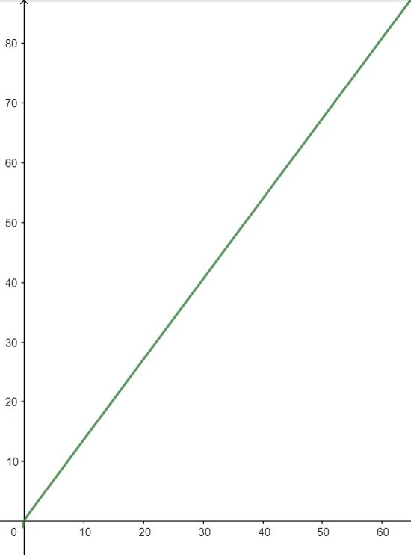
\includegraphics[width=6.906cm,height=9.3cm]{figures/Math_oraux-7.pdf}
  \caption{Graphe de la fonction $r \longmapsto \sqrt{95 r^2 + 75 r + 11} -
  \sqrt{41 r^2 + 33 r + 5} - 2 r - 1$}
\end{figure}


\

\

Donc, pour tout $n \geqslant 23 r^2 + 19 r + 3$, on a :
\[
\left( - (4r + 1) + \sqrt{4n + 3r^2 - r - 1} \right) - 
\left( - (2r + 1) + \sqrt{2n - 5r^2 - 5r - 1} \right) \geq 1
\]



Le probl{\`e}me est compl{\`e}tement r{\'e}solu.

\

Maintenant, pour aller plus loin et rendre ce probl{\`e}me plus difficile,
nous proposons les d{\'e}fis suivants :

\

\tmtextbf{Quelques d{\'e}fis.}

\tmtextbf{D{\'e}fi 1.}

$\star$ Soit $r > 1$ un entier, trouvez le plus petit entier $f (r)$ tel que,
pour tout $n \geqslant f (r)$, si l'on {\'e}crit les nombres $n, n + 1,
\ldots, 2 n$ chacun sur une carte diff{\'e}rente, puis que l'on m{\'e}lange
ces $n + 1$ cartes et qu'on les divise en deux tas, alors il existe $r$ cartes
dans l'un des tas dont la somme des nombres est un carr{\'e} parfait.

\

\tmtextbf{D{\'e}fi 2.}

$\star$ Soient $r, s > 1$ deux entiers. Trouvez le plus petit entier $g(r, s)$ tel que, pour tout $n \geqslant g(r, s)$, si l'on écrit les nombres $n, n + 1, \ldots, n + s$ chacun sur une carte diff{\'e}rente, puis que l'on
m{\'e}lange ces $s + 1$ cartes et qu'on les divise en deux tas, alors il
existe $r$ cartes dans l'un des tas dont la somme des nombres est un carr{\'e}
parfait.

\

\tmtextbf{D{\'e}fi 3.}

$\star$ Soient $r, s, t, v, w > 1$ cinq entiers, trouvez le plus petit entier
$h (r, s, t, v, w)$ tel que, pour tout $n \geqslant h (r, s, t, v, w)$, si
l'on {\'e}crit les nombres $n, n + 1, \ldots, n + s$ chacun sur une carte
diff{\'e}rente, puis que l'on m{\'e}lange ces $s + 1$ cartes et qu'on les
divise en $t$ tas, alors il existe $v$ cartes dans l'un des tas dont la somme
des nombres est une puissance parfaite de $w$.


% partie 4
\newpage
\part{Sujets d'{\'e}tude}

\

Cette partie explore quatre sujets complexes en math{\'e}matiques, chacun
abordant un domaine distinct et fondamental :
\begin{enumerate}
  \item {\textbf{Probabilit{\'e} que des entiers soient premiers entre eux}}
  : ce sujet se concentre sur la probabilit{\'e} d'obtenir des entiers
  premiers entre eux dans un ensemble donn{\'e}, en utilisant des concepts de
  la th{\'e}orie des probabilit{\'e}s et des m{\'e}thodes combinatoires.
  
  \item {\textbf{Les polyn{\^o}mes irr{\'e}ductibles sur un corps fini}} :
  ce sujet analyse le nombre de polyn{\^o}mes irr{\'e}ductibles dans un corps
  fini, un aspect essentiel de l'alg{\`e}bre et de la th{\'e}orie des corps,
  avec des applications potentielles en cryptographie et dans les structures
  alg{\'e}briques.
  
  \item {\textbf{Distribution des puissances d'un nombre dans une base de
  num{\'e}ration}} : ce sujet examine la mani{\`e}re dont les puissances d'un
  nombre se r{\'e}partissent dans une base sp{\'e}cifique, en analysant les
  fr{\'e}quences d'apparition des chiffres en premi{\`e}re position selon une
  approche probabiliste.
  
  \item {\textbf{Th{\'e}or{\`e}me de Dirichlet sur les progressions
  arithm{\'e}tiques}} : ce th{\'e}or{\`e}me fondamental en th{\'e}orie des
  nombres d{\'e}montre l'existence d'une infinit{\'e} de nombres premiers dans
  certaines progressions arithm{\'e}tiques, abordant la r{\'e}partition des
  nombres premiers, un sujet de grande importance en math{\'e}matiques pures
  et appliqu{\'e}es.
\end{enumerate}
\newpage
\begin{center}
\subsection*{Sujet 1 : Probabilit{\'e} que $l$ entiers soient premiers entre eux.}\label{sjt1}
\textbf{SABIR Ilyass}
\end{center}
\[ \star \star \star \]
\addcontentsline{toc}{subsection}{Sujet 1 : Probabilit{\'e} que $l$ entiers soient premiers entre eux.}
Soit $l \in \mathbb{N}^{\star}$, notons \tmcolor{red}{$\tmcolor{black}{\Omega
= \left( {{\mathbb{N}^{\ast}}^{} }^{^{}} \right)^l}$} , nous consid{\'e}rons
l'espace probabiliste $\tmcolor{red}{\tmcolor{black}{(\Omega, \mathcal{P}
(\Omega), \mathbb{P})}}$ , o{\`u} $\mathbb{P}$ est la fonction de masse de
probabilit{\'e} d{\'e}finie par :
\[ \mathbb{P}: I \in \mathcal{P} (\Omega) \longmapsto \underset{n \rightarrow
   + \infty}{\lim} \frac{\tmop{card} \left( I \bigcap \Omega_n \right)}{n^l}
   \in [0, 1] \]

o{\`u} $\Omega_n = {\llbracket 1, n \rrbracket^{} }^{ l}$.

Notons
\[ A_l = \left\{ (a_1, a_2, \ldots, a_l) \in \mathbb{N}_{\ast}^l  | \nobracket
   \underset{k = 1}{\overset{l}{\wedge}} a_k = 1 \right\} \]
et pour tout $n \geqslant 1$,
\[ A_{n, l} = \left\{ (a_1, a_2, \ldots, a_l) \in \llbracket 1, n \rrbracket^l
   | \nobracket  \underset{k = 1}{\overset{l}{\wedge}} a_k = 1 \right\} \]


Soient $p_1, \ldots, p_k$ des nombres premiers inf{\'e}rieurs {\`a} $n$, et
$(U_i)_{i \in \llbracket 1, k \rrbracket}$ une famille d'ensembles d{\'e}finie
pour tout $i \in \llbracket 1, k \rrbracket$ par :
\[ U_i = \{ (a_1, a_2, \ldots, a_l) \in \llbracket 1, n \rrbracket^l  |
   \nobracket \forall j \in \llbracket 1, l \rrbracket, p_i | a_j \nobracket
   \} \]


Nous pouvons facilement constater que :
\[ A_{l, n} = \overline{\underset{i = 1}{\overset{k}{\bigcup}} U_i} \]


Pour calculer la cardinalit{\'e}, nous utiliserons le principe d'inclusion-exclusion.

\

\subparagraph{Lemme 1. (Formule de Poincar{\'e})}

Soient $E_1, \ldots, E_n$ des ensembles finis, alors :
\[ \# \left( \underset{i = 1}{\overset{n}{\bigcup}} E_i \right) =
   \underset{}{\overset{n}{\underset{k = 1}{\sum}} \underset{1 \leqslant i_1 <
   \cdots < i_k \leqslant n}{\sum} (- 1)^{k - 1} \# \left(
   \overset{k}{\underset{j = 1}{\bigcap}} E_{i_j} \right)} \]

\subparagraph{Preuve du lemme 1.}

Pour $n \geqslant 2$, la preuve pour $n = 2$ a d{\'e}j{\`a} {\'e}t{\'e} vue.
Supposons que la formule est vraie pour $n$, montrons-la pour $n + 1$.

En appliquant d'abord le cas $n = 2$, puis la distributivit{\'e} des
intersections, on obtient :
\begin{eqnarray*}
  \# \left( \underset{i = 1}{\overset{n + 1}{\bigcup}} E_i \right) & = & \#
  \left( \left( \underset{i = 1}{\overset{n}{\bigcup}} E_i \right) \bigcup
  E_{n + 1} \right)\\
  & = & \# \left( \underset{i = 1}{\overset{n}{\bigcup}} E_i \right) +\#
  (E_{n + 1}) -\# \left( \left( \underset{i = 1}{\overset{n}{\bigcup}} E_i
  \right) \bigcap E_{n + 1} \right)\\
  & = & \# \left( \underset{i = 1}{\overset{n}{\bigcup}} E_i \right) +\#
  (E_{n + 1}) -\# \left( \left( \underset{i = 1}{\overset{n}{\bigcup}} \right.
  \left( E_i \bigcap E_{n + 1} \right) \right)
\end{eqnarray*}


\

Les premiers et derniers termes sont des unions $n$, pour lesquelles nous
avons suppos{\'e} la formule vraie. Par cons{\'e}quent, nous pouvons conclure.

\


\[ \# \left( \underset{i = 1}{\overset{n}{\bigcup}} E_i \right) =
   \underset{}{\overset{n}{\underset{k = 1}{\sum}} \underset{1 \leqslant i_1 <
   \cdots < i_k \leqslant n}{\sum} (- 1)^{k - 1} \# \left(
   \overset{k}{\underset{j = 1}{\bigcap}} E_{i_j} \right)} \]


Et
\[ \# \left( \left( \underset{i = 1}{\overset{n}{\bigcup}} \right. \left( E_i
   \bigcap E_{n + 1} \right) \right) = \overset{n}{\underset{k = 1}{\sum}}
   \underset{1 \leqslant i_1 < \cdots < i_k \leqslant n}{\sum} (- 1)^{k - 1}
   \# \left( \overset{k}{\underset{j = 1}{\bigcap}} \left( E_{i_j} \bigcap
   E_{n + 1} \right) \right) \]


Alors
\begin{eqnarray*}
\#\Bigl(\bigcup_{i=1}^{n+1} E_i\Bigr)
& = &
\sum_{k=1}^{n} \sum_{1 \le i_1 < \cdots < i_k \le n} (-1)^{\,k-1} \#\Bigl(\bigcap_{j=1}^{k} E_{i_j}\Bigr)
+ \#(E_{n+1}) \\[1mm]
& & + \sum_{k=1}^{n} \sum_{1 \le i_1 < \cdots < i_k \le n} (-1)^{\,k} \#\Bigl(\bigcap_{j=1}^{k} \Bigl(E_{i_j} \cap E_{n+1}\Bigr)\Bigr)
\end{eqnarray*}


Le c{\^o}t{\'e} droit peut {\^e}tre r{\'e}{\'e}crit comme
\begin{eqnarray*}
  &  & \overset{n}{\underset{k = 1}{\sum}} \underset{1 \leqslant i_1 < \cdots
  < i_k \leqslant n}{\sum} (- 1)^{k - 1} \# \left( \overset{k}{\underset{j =
  1}{\bigcap}} E_{i_j} \right) +\# (E_{n + 1})\\
  & = & \overset{n + 1}{\underset{k = 1}{\sum}} \underset{i_k \neq n +
  1}{\underset{1 \leqslant i_1 < \cdots < i_k \leqslant n + 1}{\sum}} (- 1)^{k
  - 1} \# \left( \overset{k}{\underset{j = 1}{\bigcap}} E_{i_j} \right) +
  \overset{n + 1}{\underset{k = 1}{\sum}} \# (E_k)
\end{eqnarray*}


Et
\begin{eqnarray*}
  &  & \overset{n}{\underset{k = 1}{\sum}} \underset{1 \leqslant i_1 < \cdots
  < i_k \leqslant n}{\sum} (- 1)^k \# \left( \overset{k}{\underset{j =
  1}{\bigcap}} \left( E_{i_j} \bigcap E_{n + 1} \right) \right)\\
  & = & \overset{n + 1}{\underset{k = 2}{\sum}} \underset{i_k = n +
  1}{\underset{1 \leqslant i_1 < \cdots < i_k < i_k \leqslant n + 1}{\sum}} (-
  1)^{k - 1} \# \left( \overset{k}{\underset{j = 1}{\bigcap}} E_{i_j} \right)
\end{eqnarray*}


Nous concluons que


\[
\begin{aligned}
\#\Biggl(\bigcup_{i=1}^{n+1} E_i\Biggr)
&= \sum_{k=1}^{n+1} \#(E_k)
+ \sum_{k=1}^{n+1} \Biggl[
\sum_{\substack{1\le i_1<\cdots<i_k\le n+1 \\ i_k\neq n+1}} (-1)^{\,k-1}\,\#\Bigl(\bigcap_{j=1}^k E_{i_j}\Bigr)\\[1ex]
&\quad + \sum_{\substack{1\le i_1<\cdots<i_k\le n+1 \\ i_k = n+1}} (-1)^{\,k-1}\,\#\Bigl(\bigcap_{j=1}^k E_{i_j}\Bigr)
\Biggr].
\end{aligned}
\]



Ainsi,
\[ \# \left( \underset{i = 1}{\overset{n + 1}{\bigcup}} E_i \right) =
   \underset{}{\overset{n + 1}{\underset{k = 1}{\sum}} \underset{1 \leqslant
   i_1 < \cdots < i_k \leqslant n + 1}{\sum} (- 1)^{k - 1} \# \left(
   \overset{k}{\underset{j = 1}{\bigcap}} E_{i_j} \right)} \]


ce qui justifie la formule pour $n + 1$.

\subparagraph{D{\'e}finition 1. (La fonction de M{\"o}bius)}

Soit $n \in \mathbb{N}^{\star}$, on note $\mu (n)$ l'entier d{\'e}fini par :
\[
\mu(n) =
\begin{cases}
0, & \text{si } n \text{ possède un facteur premier au carré},\\[1mm]
1, & \text{si } n \text{ est sans facteur premier au carré et a un nombre pair de facteurs premiers},\\[1mm]
-1, & \text{si } n \text{ est sans facteur premier au carré et a un nombre impair de facteurs premiers}.
\end{cases}
\]



D'apr{\`e}s le lemme 1, on a

\[  \]
\[ \# \left( \underset{i = 1}{\overset{k}{\bigcup}} U_i \right) =
   \overset{k}{\underset{j = 1}{\sum}} \underset{1 \leqslant i_1 < \cdots <
   i_j \leqslant k}{\sum} (- 1)^{j - 1} \# \left( \overset{j}{\underset{m =
   1}{\bigcap}} U_{i_m} \right) \]


Pour conclure, il suffit de calculer $\overset{j}{\underset{m = 1}{\bigcap}}
U_{i_m}$, pour tout $\leqslant i_1 < \cdots < i_j \leqslant k$

\

Soit $I \subset \llbracket 1, k \rrbracket$ non vide, le cardinal de
l'intersection $\underset{i \in I}{\bigcap} U_i$ est {\'e}gal au nombre des
$l$-uplets de multiples strictement positifs de $\underset{i \in I}{\prod}
p_i$ inf{\'e}rieurs ou {\'e}gaux {\`a} $n$, ce cardinal est {\'e}gal {\`a} :
\tmcolor{red}{$\tmcolor{black}{\left\lfloor \frac{n}{\underset{i \in I}{\prod}
p_i} \right\rfloor^l}$}.

\

La formule de Poincar{\'e} donne :
\[ \# \left( \underset{i = 1}{\overset{k}{\bigcup}} U_i \right) =
   \overset{k}{\underset{j = 1}{\sum}} \underset{1 \leqslant i_1 < \cdots <
   i_j \leqslant k}{\sum} (- 1)^{j - 1} \left\lfloor
   \frac{n}{\overset{j}{\underset{m = 1}{\prod}} p_{i_m}} \right\rfloor^l \]


Par cons{\'e}quent,
\[ \#A_{l, n} = n^l -\# \left( \underset{i = 1}{\overset{k}{\bigcup}} U_i
   \right) = \underset{d = 1}{\overset{n}{\sum}} \mu (d) \left\lfloor
   \frac{n}{d} \right\rfloor^l \]


Donc,
\[ \tmcolor{red}{\tmcolor{black}{\frac{\# (A_{l, n})}{n^l} = \frac{1}{n^l}
   \underset{d = 1}{\overset{n}{\sum}} \mu (d) \left\lfloor \frac{n}{d}
   \right\rfloor^l}} \]


Pour continuer la d{\'e}monstration, nous avons besoin d'une propri{\'e}t{\'e}
fondamentale de la fonction de M{\"o}bius.

\subparagraph{Proposition 1.}

Pour tout entier $n \neq 1$, on a
\[ \underset{d | \nobracket n}{\sum} \mu (d) = 0 \]

\subparagraph{Preuve.}

\tmtextbf{M{\'e}thode 1.} Soit $n = \underset{i = 1}{\overset{m}{\prod}}
p^{a_i}_i$ la d{\'e}composition en facteurs premiers de $n$, et $d \in
\mathbb{N}$, on a:

$d | \nobracket n \infixand \mu (d) \neq 0$ si et seulement si $d =
\underset{i \in J}{\overset{}{\prod}} p^{a_i}_i$ avec $J \subset \llbracket 1,
m \rrbracket$. Donc
\[ \mu (d) = (- 1)^{\#J} \]


Par suite,
\begin{eqnarray*}
  \underset{d | \nobracket n}{\sum} \mu (d) & = & \underset{J \subset
  \llbracket 1, m \rrbracket}{\sum} (- 1)^{\#J}\\
  & = & (1 - 1)^m\\
  & = & 0 \quad (\tmop{car} m > 0)
\end{eqnarray*}


\tmtextbf{M{\'e}thode 2.} Soit $n \geqslant 2$. D'apr{\`e}s le
th{\'e}or{\`e}me fondamental de l'arithm{\'e}tique, il existe des entiers
premiers $(p_1, \ldots, p_r) \in \mathcal{P}^r$ et des entiers $\alpha_1,
\ldots, \alpha_r \geqslant 1$ tels que $n = \underset{i =
1}{\overset{r}{\prod}} p^{\alpha_i}_i$

On a alors :
\[ \underset{d | \nobracket n}{\sum} \mu (d) = \underset{k_1 =
   0}{\overset{\alpha_1}{\sum}} \underset{k_2 = 0}{\overset{\alpha_2}{\sum}}
   \ldots \underset{k_r = 0}{\overset{\alpha_r}{\sum}} \mu \left( \underset{i
   = 1}{\overset{r}{\prod}} p^{k_i}_i \right) \]


Donc :
\[ \underset{d | \nobracket n}{\sum} \mu (d) = \underset{\exists i_0 \in
   \llbracket 1, r \rrbracket k_{i_0} \geqslant 2}{\underset{(k_1, \ldots,
   k_r) \in \underset{i = 1}{\overset{r}{\prod}} \llbracket 0, \alpha_i
   \rrbracket}{\overset{}{\sum}}} \mu \left( \underset{i =
   1}{\overset{r}{\prod}} p^{k_i}_i \right) + \underset{}{\underset{(k_1,
   \ldots, k_r) \in \llbracket 0, 1 \rrbracket^r}{\overset{}{\sum}}} \mu
   \left( \underset{i = 1}{\overset{r}{\prod}} p^{k_i}_i \right) \]


Puisque pour tout $(k_1, \ldots, k_r) \in \underset{i = 1}{\overset{r}{\prod}}
\llbracket 0, \alpha_i \rrbracket$ tel qu'il existe $i_0 \in \llbracket 1, r
\rrbracket$ avec $k_{i_0} \geqslant 2$, alors $\underset{i =
1}{\overset{r}{\prod}} p^{k_i}_i$ est divisible par $p^2_{i_0 }$, donc
\[ \mu \left( \underset{i = 1}{\overset{r}{\prod}} p^{k_i}_i \right) = 0 \]


Ce qui implique que :
\[ \underset{\exists i_0 \in \llbracket 1, r \rrbracket k_{i_0} \geqslant
   2}{\underset{(k_1, \ldots, k_r) \in \underset{i = 1}{\overset{r}{\prod}}
   \llbracket 0, \alpha_i \rrbracket}{\overset{}{\sum}}} \mu \left(
   \underset{i = 1}{\overset{r}{\prod}} p^{k_i}_i \right) = 0 \]


Par cons{\'e}quent :
\[ \underset{d | \nobracket n}{\sum} \mu (d) = \underset{}{\underset{(k_1,
   \ldots, k_r) \in \llbracket 0, 1 \rrbracket^r}{\overset{}{\sum}}} \mu
   \left( \underset{i = 1}{\overset{r}{\prod}} p^{k_i}_i \right) \]


Pour tout $(k_1, \ldots, k_r) \in \llbracket 0, 1 \rrbracket^r$, on a
$\overset{r}{\underset{i = 1}{\sum}} k_i$ est le nombre de facteurs premiers
distincts de

$\underset{i = 1}{\overset{r}{\prod}} p^{k_i}_i$, et $\underset{i =
1}{\overset{r}{\prod}} p^{k_i}_i$ n'est pas divisible par le carr{\'e} d'un
nombre premier. Ainsi :
\begin{eqnarray*}
  \underset{d | \nobracket n}{\sum} \mu (d) & = & \underset{}{\underset{(k_1,
  \ldots, k_r) \in \llbracket 0, 1 \rrbracket^r}{\overset{}{\sum}}} (-
  1)^{\overset{r}{\underset{i = 1}{\sum}} k_i}\\
  & = & \underset{i = 1}{\overset{r}{\prod}} \left( \underset{k_1 =
  0}{\overset{1 }{\sum}} (- 1)^{k_i} \right)\\
  & = & (1 - 1)^r\\
  & = & 0
\end{eqnarray*}


\

Pour l'{\'e}tude asymptotique de $\frac{\# (A_{l, n})}{n^l}$, il semble
naturel de remplacer le terme $\frac{1}{n^l} \left\lfloor \frac{n}{d}
\right\rfloor^l$ par son {\'e}quivalent $\frac{1}{d^l}$. La diff{\'e}rence
entre les deux sommes s'{\'e}crit :
\[ \left| \frac{\# (A_{l, n})}{n^l} - \underset{d = 1}{\overset{n}{\sum}}
   \frac{\mu (d)}{d^l} \right| = \left| \underset{d = 1}{\overset{n}{\sum}}
   \mu (d) \left( \frac{1}{n^l} \left\lfloor \frac{n}{d} \right\rfloor^l -
   \frac{1}{d^l} \right) \right| \]


Comme $\left\lfloor \frac{n}{d} \right\rfloor  > \frac{n}{d} - 1$, On a
\begin{eqnarray*}
  \underset{k = 1}{\overset{l}{\sum}} \begin{array}{c}
    \\
    
  \end{array} \left( \begin{array}{c}
    l\\
    k
  \end{array} \right) \frac{1}{d^k n^{l - k}} & = & \left( \frac{1}{d} -
  \frac{1}{n} \right)^l - \frac{1}{d^l}\\
  & < & \frac{1}{n^l} \left\lfloor \frac{n}{d} \right\rfloor^l -
  \frac{1}{d^l}\\
  & \leqslant & 0
\end{eqnarray*}


Ce qui donne
\begin{eqnarray*}
  \left| \frac{\# (A_{l, n})}{n^l} - \underset{d = 1}{\overset{n}{\sum}}
  \frac{\mu (d)}{d^l} \right| & \leqslant & \underset{d =
  1}{\overset{n}{\sum}} \underset{k = 1}{\overset{l}{\sum}} \begin{array}{c}
    \\
    
  \end{array} \left( \begin{array}{c}
    l\\
    k
  \end{array} \right) \frac{1}{d^k n^{l - k}}\\
  & = & \underset{k = 1}{\overset{l}{\sum}} \begin{array}{c}
    \\
    
  \end{array} \left( \begin{array}{c}
    l\\
    k
  \end{array} \right) \frac{1}{n^{l - k}} \left( \underset{d =
  1}{\overset{n}{\sum}} \frac{1}{d^k } \right)
\end{eqnarray*}


Ainsi,
\begin{eqnarray*}
  \underset{k = 1}{\overset{l}{\sum}} \begin{array}{c}
    \\
    
  \end{array} \left( \begin{array}{c}
    l\\
    k
  \end{array} \right) \frac{1}{n^{l - k}} \left( \underset{d =
  1}{\overset{n}{\sum}} \frac{1}{d^k } \right) & \underset{n \rightarrow +
  \infty}{\sim} & \left( \begin{array}{c}
    l\\
    1
  \end{array} \right) \frac{1}{n^{l - 1}} \log (n) + \underset{k =
  2}{\overset{l}{\sum}} \begin{array}{c}
    \\
    
  \end{array} \left( \begin{array}{c}
    l\\
    k
  \end{array} \right) \frac{1}{n^{l - k}} \underset{d = 1}{\overset{+
  \infty}{\sum}} \frac{1}{d^k }\\
  & = & O \left( \frac{1}{n^{l - 1}} \log (n) \right)
\end{eqnarray*}


Par suite,
\[ \mathbb{P} (A_l) = \underset{n \rightarrow + \infty}{\lim} \frac{\# (A_{l,
   n})}{n^l} = \underset{d = 1}{\overset{+ \infty}{\sum}} \frac{\mu (d)}{d^l}
\]


\subparagraph{D{\'e}finition 2.}

On d{\'e}finit la fonction z{\^e}ta de Riemann, pour tout $z \in \mathbb{C}$
tel que $\tmop{Re} (z) > 1$, par
\[ \zeta (z) = \underset{n = 1}{\overset{+ \infty}{\sum}} \frac{1}{n^z} \]


\subparagraph{Proposition 2.}

Pour tout nombre complexe $z$ tel que $\tmop{Re} (z) > 1$, on a :
\[ \frac{1}{\zeta (z)} = \underset{n = 1}{\overset{+ \infty}{\sum}} \frac{\mu
   (n)}{n^z} \]

\subparagraph{Preuve.}

Soit $z \in \mathbb{C}$, tel que $\tmop{Re} (z) > 1$,on a, via la proposition
1 :
\begin{eqnarray*}
  \zeta (z) . \underset{n = 1}{\overset{+ \infty}{\sum}} \frac{\mu (n)}{n^z} &
  = & \left( \underset{n = 1}{\overset{+ \infty}{\sum}} \frac{1}{n^z} \right)
  \left( \underset{n = 1}{\overset{+ \infty}{\sum}} \frac{\mu (n)}{n^z}
  \right)\\
  & = & \underset{n, d \geqslant 1}{\overset{}{\sum}} \frac{\mu
  (d)}{(n.d)^z}\\
  & = & \underset{n \geqslant 1}{\overset{}{\sum}} \underset{d | n
  \nobracket}{\overset{}{\sum}} \frac{\mu (d)}{n^z}\\
  & = & 1
\end{eqnarray*}


On en conclut que
\[ \mathbb{P} (A_l) = \frac{1}{\zeta (l)} \]


\subparagraph{Remarque 1.}

On peut d{\'e}duire directement de ce r{\'e}sultat le th{\'e}or{\`e}me d'Euclide, qui {\'e}nonce que l'ensemble des nombres premiers est infini.
\newpage
\begin{center}
\subsection*{Sujet 2 : Les polyn{\^o}mes irr{\'e}ductibles sur $K [X]$.}\label{sjt2}
\textbf{SABIR Ilyass}
\end{center}
\[ \star \star \star \]
\addcontentsline{toc}{subsection}{Sujet 2 : Les polyn{\^o}mes irr{\'e}ductibles sur $K [X]$.}
\paragraph{L'objectif.}

Soit $K$ un corps commutatif fini, on veut trouver le nombre des polyn{\^o}mes
irr{\'e}ductibles sur $K [X]$ de degr{\'e} $n$.
\[ \star \star \star \star \star \star \star \star \star \star \]


\tmtextbf{Th{\'e}or{\`e}me 1.}

Il existe un nombre premier $p$ et un entier $n \in \mathbb{N}$, tel que
\[ \#K = p^n \]


\tmtextbf{Preuve du th{\'e}or{\`e}me 1.}

\

Notons $L$ le plus petit sous corps de $K$.

Puisque $K$ est fini, alors il existe un nnombre premier $p$ tel que $L$ est
isomorphe {\`a} $\mathbb{Z}/ p\mathbb{Z}$, en particulier $\#L = p$.

On note :
\begin{eqnarray*}
  n & \assign & [K : \mathbb{Z}/ p\mathbb{Z}]\\
  & = & \dim_L (K)\\
  & < & + \infty
\end{eqnarray*}


$K$est un $L$ espace-vectoriel de dimension $n$. Notons $\mathcal{B}= (e_1,
\ldots, e_n)$ une base de $K$ comme $L$espace-vectoriel. De plus l'application
:
\[ \begin{array}{ccc}
     L^n & \rightarrow & K\\
     (x_1, \ldots, x_n) & \longmapsto & \underset{k = 1}{\overset{n}{\sum}}
     x_k e_k
   \end{array} \]


est bijective, en particulier :
\begin{eqnarray*}
  \#K & = & \# (L^n)\\
  & = & p^n
\end{eqnarray*}
\[ \star \star \star \star \star \star \star \star \star \star \]


On note pour tout entier $n \in \mathbb{N}^{\ast}$, $\mathcal{P}_K (n)$
l'ensemble des polyn{\^o}mes unitaires irr{\'e}ductibles de degr{\'e} $n$ sur
$K [X]$.

Pour tout polyn{\^o}me $P \in K [X]$ irr{\'e}ductible, et pour tout $a \in K
\backslash \nobracket \{ 0 \}$ $a.P$ est {\'e}galement irr{\'e}ductible sur $K
[X]$.

On a donc, pour tout entier $n \in \mathbb{N}^{\ast}$, le nombre de
polyn{\^o}mes irr{\'e}ductibles de degr{\'e} $n$ est :
\[ (\#K - 1) .\#\mathcal{P}_K (n) \]


Il ne reste plus qu'{\`a} trouver le cardinal de $\mathcal{P}_K (n)$ pour tout
$n \in \mathbb{N}^{\ast}$.

\

\tmtextbf{Th{\'e}or{\`e}me 2.}

Notons $\#K = q$. Soit $n \in \mathbb{N}^{\ast}$, on a
\[ X^{q^n} - X = \underset{d | n \nobracket}{\prod}  \underset{P \in
   \mathcal{P}_K (d)}{\prod} P (X) \]


\tmtextbf{Preuve du th{\'e}or{\`e}me 2.}

Pour tout entier $d \in \mathbb{N}^{\ast}$ et pour tout $P \in \mathcal{P}_K
(d),$ on a $M = K / (P)$ est un corps (car $K$ est principal), de cardinal
$q^d$ , donc isomorphe {\`a} $\mathbb{Z}/ q^d \mathbb{Z}$. Ainsi, pour tout $x
\in M$ :
\[ x^{q^d} = x \]


Mais si $n = d.k$ pour un $k \in \mathbb{N}^{\ast}$, on a \
\[ x^{q^n} = x^{q^{d.k}} = (((x^{q^d})^{q^d}) \ldots)^{q^d} \quad (k
   \tmop{fois}) \]


Par une r{\'e}currence imm{\'e}diate sur $k$, ceci est {\'e}gal {\`a} $x$.
Autrement dit,
\[ X^{q^n} \nonconverted{minus} X = 0 \in M [X] \]


Donc $P$ divise $X^{q^n} \nonconverted{minus} X$ dans $K [X]$.

Comme les {\'e}l{\'e}ments de $\mathcal{P}_K (d)$ sont irr{\'e}ductibles, le
produit $\underset{d | n \nobracket}{\prod}  \underset{P \in \mathcal{P}_K
(d)}{\prod} P (X)$ divise lui aussi $X^{q^n} \nonconverted{minus} X$.

R{\'e}ciproquement, soit $P$ un facteur irr{\'e}ductible de degr{\'e} $d$ de
$X^{q^n} \nonconverted{minus} X$ dans $K [X$].

Comme $\mathbb{Z}/ q^n \mathbb{Z}$ est un corps de d{\'e}composition de
$X^{q^n} \nonconverted{minus} X$, $P$ est scind{\'e} sur $\mathbb{Z}/ q^n
\mathbb{Z}$.

Si $x$ est une racine de $P$, on a
\begin{eqnarray*}
  {}[\mathbb{Z}/ q^n \mathbb{Z}: \mathbb{Z}/ q\mathbb{Z}] & = & n\\
  & = & [\mathbb{Z}/ q^n \mathbb{Z}: \mathbb{Z}/ q\mathbb{Z}(x)] [\mathbb{Z}/
  q\mathbb{Z}(x) : \mathbb{Z}/ q\mathbb{Z}]
\end{eqnarray*}


Mais comme $P$ est irr{\'e}ductible, $\mathbb{Z}/ q\mathbb{Z}(x)$ est un corps
de rupture de $P$ de degr{\'e} $d$ sur $\mathbb{Z}/ q\mathbb{Z}$, donc d
divise $n$.

Il suffit alors de montrer que $X^{q^n} \nonconverted{minus} X$ n'admet pas
de facteur double (ou plus). En effet, si un tel facteur existe, alors
$X^{q^n} \nonconverted{minus} X$ admet une racine double dans un corps de
d{\'e}composition.

Cependant, comme le polyn{\^o}me d{\'e}riv{\'e} de $X^{q^n}
\nonconverted{minus} X$ est $q^n X^{q^n - 1} \nonconverted{minus} 1 = - 1$
({\`a} cause de la caract{\'e}ristique), $X^{q^n} \nonconverted{minus} X$ n'a
pas de racine double dans un corps de d{\'e}composition, ce qui termine la
preuve.

\

\tmtextbf{D{\'e}finition 1. (La fonction de M{\"o}bius)}

Soit $n \in \mathbb{N}^{\ast}$. On note $\mu (n)$ l'entier d{\'e}fini par :
\[ \mu (n) = \left\{\begin{array}{l}
     0 \quad \tmop{si} n \tmop{est} \tmop{divisible} \tmop{par} \tmop{le}
     \tmop{carr} {\'e} d\prime \tmop{un} \tmop{nombre} \tmop{premier}\\
     (- 1)^r \quad \tmop{si} r \tmop{est} \tmop{le} \tmop{nombre} \tmop{de}
     \tmop{facteurs} \tmop{premiers} \tmop{distincts} \tmop{de} n,\\
     n \tmop{non} \tmop{divisible} \tmop{par} \tmop{le} \tmop{carr} {\'e}
     d\prime \tmop{un} \tmop{nombre} \tmop{premier}
   \end{array}\right. \]


\

\tmtextbf{Proposition 1.}

pour tout $n \neq 1$, on a l'{\'e}galit{\'e} :
\[ \underset{d | \nobracket n}{\sum} \mu (d) = 0 \]


\tmtextbf{Preuve de la proposition 1.}

\tmtextbf{M{\'e}thode 1.}

Soit $n = \underset{i = 1}{\overset{m}{\prod}} p^{a_i}_i$ la
d{\'e}composition en facteurs premiers de $n$.



De plus si $d \in \mathbb{N}$, alors :

$d$divise $n \infixand \mu (d) \neq 0$ si et seulement si $d = \underset{i \in
J}{\overset{}{\prod}} p^{a_i}_i$ with $J \subset \llbracket 1, m \rrbracket$
et alors
\[ \mu (d) = (- 1)^{\#J} \]


On en d{\'e}duit que :
\begin{eqnarray*}
  \underset{d | \nobracket n}{\sum} \mu (d) & = & \underset{J \subset
  \llbracket 1, m \rrbracket}{\sum} (- 1)^{\#J}\\
  & = & (1 - 1)^m\\
  & = & 0 \qquad (\tmop{car} m > 0)
\end{eqnarray*}


\tmtextbf{M{\'e}thode 2.}

Soit $n \geqslant 2$. D'apr{\`e}s le th{\'e}or{\`e}me fondamentale d
l'arithm{\'e}tique, il existe $(p_1, \ldots, p_r) \in \mathcal{P}^r$ et
$\alpha_1, \ldots, \alpha_r \geqslant 1$ tels que
\[ n = \underset{i = 1}{\overset{r}{\prod}} p^{\alpha_i}_i \]


On a
\begin{eqnarray*}
  \underset{d | \nobracket n}{\sum} \mu (d) & = & \underset{k_1 =
  0}{\overset{\alpha_1}{\sum}} \underset{k_2 = 0}{\overset{\alpha_2}{\sum}}
  \ldots \underset{k_r = 0}{\overset{\alpha_r}{\sum}} \mu \left( \underset{i =
  1}{\overset{r}{\prod}} p^{k_i}_i \right)\\
  & = & \underset{\exists i_0 \in \llbracket 1, r \rrbracket k_{i_0}
  \geqslant 2}{\underset{(k_1, \ldots, k_r) \in \underset{i =
  1}{\overset{r}{\prod}} \llbracket 0, \alpha_i \rrbracket}{\overset{}{\sum}}}
  \mu \left( \underset{i = 1}{\overset{r}{\prod}} p^{k_i}_i \right) +
  \underset{}{\underset{(k_1, \ldots, k_r) \in \llbracket 0, 1
  \rrbracket^r}{\overset{}{\sum}}} \mu \left( \underset{i =
  1}{\overset{r}{\prod}} p^{k_i}_i \right)
\end{eqnarray*}


Puisque pour tout $(k_1, \ldots, k_r) \in \underset{i = 1}{\overset{r}{\prod}}
\llbracket 0, \alpha_i \rrbracket$ tel qu'il existe $i_0 \in \llbracket 1, r
\rrbracket \tmop{avec} k_{i_0} \geqslant 2$, on a :
\[ \underset{i = 1}{\overset{r}{\prod}} p^{k_i}_i \tmop{est} \tmop{divisible}
   \tmop{par} p^2_{i_0 } \]


Alors,
\[ \mu \left( \underset{i = 1}{\overset{r}{\prod}} p^{k_i}_i \right) = 0 \]


D'o{\`u}
\[ \underset{\exists i_0 \in \llbracket 1, r \rrbracket k_{i_0} \geqslant
   2}{\underset{(k_1, \ldots, k_r) \in \underset{i = 1}{\overset{r}{\prod}}
   \llbracket 0, \alpha_i \rrbracket}{\overset{}{\sum}}} \mu \left(
   \underset{i = 1}{\overset{r}{\prod}} p^{k_i}_i \right) = 0 \]


Par suite
\[ \underset{d | \nobracket n}{\sum} \mu (d) = \underset{}{\underset{(k_1,
   \ldots, k_r) \in \llbracket 0, 1 \rrbracket^r}{\overset{}{\sum}}} \mu
   \left( \underset{i = 1}{\overset{r}{\prod}} p^{k_i}_i \right) \]


Pour tout $(k_1, \ldots, k_r) \in \llbracket 0, 1 \rrbracket^r$, on a
$\overset{r}{\underset{i = 1}{\sum}} k_i$ est le nombre de facteurs premiers
distincts de $\underset{i = 1}{\overset{r}{\prod}} p^{k_i}_i$ et $\underset{i
= 1}{\overset{r}{\prod}} p^{k_i}_i$ est non divisible par le carr{\'e} d'un
nombre premier, alors
\begin{eqnarray*}
  \underset{d | \nobracket n}{\sum} \mu (d) & = & \underset{}{\underset{(k_1,
  \ldots, k_r) \in \llbracket 0, 1 \rrbracket^r}{\overset{}{\sum}}} (-
  1)^{\overset{r}{\underset{i = 1}{\sum}} k_i}\\
  & = & \underset{i = 1}{\overset{r}{\prod}} \left( \underset{k_1 =
  0}{\overset{1 }{\sum}} (- 1)^{k_i} \right)\\
  & = & (1 - 1)^r\\
  & = & 0
\end{eqnarray*}


\tmtextbf{Th{\'e}or{\`e}me 3. (La formule d'inversion de M{\"o}bius)}

\tmcolor{red}{}Soit $H$ une fonction non nulle de $\mathbb{N}^{\ast}$ dans
$\mathbb{C}$ telle que
\[ \forall n, m \in \mathbb{N}, H (n.m) = H (n) H (m) \]


On se donne {\'e}galement deux fonctions $F$ et $G$ de$[1, + \infty [$ dans
$\mathbb{C}$ telles que, pour tout $x > 1$ :
\[ {\color[HTML]{000000}{\color[HTML]{000000}G (x) = \underset{1 \leqslant k
   \leqslant x}{\sum} F \left( \frac{x}{k} \right) H (k)}} \]


Alors, pour tout $x > 1$, on a :
\[ {\color[HTML]{000000}{\color[HTML]{000000}F (x) = \underset{1 \leqslant k
   \leqslant x}{\sum} \mu (k) G \left( \frac{x}{k} \right) H (k)}} \]


\tmtextbf{Preuve du th{\'e}or{\`e}me 3.}

\tmcolor{red}{}On a
\[ H (1) = H (1 \times 1) = H (1)^2 \]


Et puisque $H \neq 0$ alors $H (1) = 1$.

Pour tout $x \in [1, + \infty [$, on a :
\begin{eqnarray*}
  \underset{1 \leqslant k \leqslant x}{\sum} \mu (k) G \left( \frac{x}{k}
  \right) H (k) & = & \underset{1 \leqslant k \leqslant x}{\sum} \mu (k)
  \underset{1 \leqslant i \leqslant \frac{x}{k}}{\sum} F \left( \frac{x}{i.k}
  \right) H (i) H (k)\\
  & = & \underset{1 \leqslant k \leqslant x}{\sum} \underset{1 \leqslant i
  \leqslant \frac{x}{k}}{\sum} \mu (k) F \left( \frac{x}{i.k} \right) H
  (i.k)\\
  & = & \underset{1 \leqslant k.i \leqslant x}{\sum} \mu (k) F \left(
  \frac{x}{i.k} \right) H (i.k)\\
  & = & \underset{1 \leqslant m \leqslant x}{\sum} \underset{d | \nobracket
  m}{\sum} \mu (d) F \left( \frac{x}{m} \right) H (m)\\
  & = & \underset{1 \leqslant m \leqslant x}{\sum} F \left( \frac{x}{m}
  \right) H (m) \left( \underset{d | \nobracket m}{\sum} \mu (d) \right)\\
  & = & (x) H (1) + \underset{2 \leqslant m \leqslant x}{\sum} F \left(
  \frac{x}{m} \right) H (m) \left( \underset{d | \nobracket m}{\sum} \mu (d)
  \right)
\end{eqnarray*}


D'apr{\`e}s la proposition 1, pour tout $m \geqslant 2$, on a :
\[ \underset{d | \nobracket m}{\sum} \mu (d) = 0 \]


D'o{\`u} :
\[ F (x) = \underset{1 \leqslant k \leqslant x}{\sum} \mu (k) G \left(
   \frac{x}{k} \right) H (k) \]


\tmtextbf{Corollaire 1.}

Pour tout entier $n \in \mathbb{N}^{\ast}$, on a :
\[ \#\mathcal{P}_K (n) = \frac{1}{n} \underset{d | n \nobracket}{\sum} \mu
   \left( \frac{n}{d} \right) (\#K)^d \]


\tmtextbf{Preuve du corollaire}

\tmcolor{red}{}Soit $n \in \mathbb{N}^{\ast}$, notons $\#K = q$. D'apr{\`e}s
th{\'e}or{\`e}me 1, on a :
\[ {\color[HTML]{000000}{\color[HTML]{000000}X^{q^n} - X = \underset{d | n
   \nobracket}{\prod}  \underset{P \in \mathcal{P}_K (d)}{\prod} P (X)}
   \tmcolor{black}{}} \]


Donc :
\begin{eqnarray*}
  q^n & = & \deg (X^{q^n} - X)\\
  & = & \underset{d | n \nobracket}{\sum}  \underset{P \in \mathcal{P}_K
  (d)}{\sum} \deg (P (X))\\
  & = & \deg \left( \underset{d | n \nobracket}{\prod}  \underset{P \in
  \mathcal{P}_K (d)}{\prod} P (X) \right)
\end{eqnarray*}


Par suite :
\[ \underset{d | n \nobracket}{\sum} d.\#\mathcal{P}_K (d) = q^n \]


D'o{\`u}, d'apr{\`e}s la formule d'inversion de M{\"o}bius :
\[ \#\mathcal{P}_K (n) = \frac{1}{n} \underset{d | n \nobracket}{\sum} \mu
   \left( \frac{n}{d} \right) (\#K)^d \]

\[ \star \star \star \star \star \star \star \star \star \star \]

\paragraph{Pour aller plus loin.}

On veut trouver le nombre de polyn{\^o}mes irr{\'e}ductibles sur $K [X]$.

On a que le nombre de polyn{\^o}mes irr{\'e}ductibles sur $K [X]$ est :
\begin{eqnarray*}
  \underset{n = 1}{\overset{+ \infty}{\sum}} (\#K - 1) .\#\mathcal{P}_K (n) &
  = & (\#K - 1) \underset{n = 1}{\overset{+ \infty}{\sum}} \#\mathcal{P}_K
  (n)\\
  & = & (\#K - 1) \underset{n = 1}{\overset{+ \infty}{\sum}} \frac{1}{n}
  \underset{d | n \nobracket}{\sum} \mu \left( \frac{n}{d} \right) (\#K)^d
\end{eqnarray*}


Pour simplifier l'{\'e}criture, on pose $\#K = q$, et on a :
\begin{eqnarray*}
  \underset{n = 1}{\overset{+ \infty}{\sum}} \frac{1}{n} \underset{d | n
  \nobracket}{\sum} \mu \left( \frac{n}{d} \right) q^d & = & \underset{n =
  1}{\overset{+ \infty}{\sum}} \underset{d | n \nobracket}{\sum} \frac{1}{n}
  \mu \left( \frac{n}{d} \right) q^d\\
  & = & \underset{n = 1}{\overset{+ \infty}{\sum}} \underset{d =
  1}{\overset{+ \infty}{\sum}} \frac{1}{n} \mu \left( \frac{n}{d} \right)
  1_{\mathbb{N}} \left( \frac{n}{d} \right) q^d
\end{eqnarray*}


$\underset{}{}$Avec $\mu (r) = 0$ pour les nombres rationnels (on d{\'e}finit
simplement un prolongement de $\mu$ qui n'a pas d'influence sur le
r{\'e}sultat de la somme, puisque $1_{\mathbb{N}} (r) = 0$si $r$ n'est pas
entier).

On a alors, d'apr{\`e}s le th{\'e}or{\`e}me de Fubini et par positivit{\'e}
des termes de la somme :
\begin{eqnarray*}
  \underset{n = 1}{\overset{+ \infty}{\sum}} \frac{1}{n} \underset{d | n
  \nobracket}{\sum} \mu \left( \frac{n}{d} \right) q^d & = & \underset{d =
  1}{\overset{+ \infty}{\sum}} \underset{n = 1}{\overset{+ \infty}{\sum}}
  \frac{1}{n} \mu \left( \frac{n}{d} \right) 1_{\mathbb{N}} \left( \frac{n}{d}
  \right) q^d\\
  & = & \underset{d = 1}{\overset{+ \infty}{\sum}} \underset{n =
  1}{\overset{+ \infty}{\sum}} \frac{1}{d.n} \mu (n) q^{d.n}\\
  & = & \underset{d = 1}{\overset{+ \infty}{\sum}} \frac{1}{d} \underset{n =
  1}{\overset{+ \infty}{\sum}} \frac{1}{n} \mu (n) (q^d)^n
\end{eqnarray*}


Pour tout entier $d \in \mathbb{N}^{\ast}$, essayons de calculer la somme de
la s{\'e}rie $\underset{n \geqslant 1}{\overset{}{\sum}} \frac{1}{n} \mu (n)
(q^d)^n$

Notons pour tout $r \in \mathbb{N}^{\star}$, $p_r$ le r-i{\`e}me nombre
premier.

On a pour tout $N \in \mathbb{N}^{\star}$, par d{\'e}finition de la fonction
de M{\"o}bius :
\begin{eqnarray*}
  \underset{n_1 = 0}{\overset{+ \infty}{\sum}}  \underset{n_2 = 0}{\overset{+
  \infty}{\sum}} \ldots \underset{n_N = 0}{\overset{+ \infty}{\sum}}
  \frac{1}{\underset{i = 1}{\overset{N}{\prod}} p^{n_i}_i} \mu \left(
  \underset{i = 1}{\overset{N}{\prod}} p^{n_i}_i \right) (q^d)^{\underset{i =
  1}{\overset{N}{\prod}} p^{n_i}_i} & = & \underset{n_1, \ldots, n_N \in \{ 0,
  1 \}}{\overset{}{\sum}} \frac{1}{\underset{i = 1}{\overset{N}{\prod}}
  p^{n_i}_i} \mu \left( \underset{i = 1}{\overset{N}{\prod}} p^{n_i}_i \right)
  (q^d)^{\underset{i = 1}{\overset{N}{\prod}} p^{n_i}_i}\\
  & = & \underset{n_1, \ldots, n_N \in \{ 0, 1 \}}{\overset{}{\sum}}
  \frac{1}{\underset{i = 1}{\overset{N}{\prod}} p^{n_i}_i} {(- 1)^{\underset{i
  = 1}{\overset{N}{\sum}} n_i}}  (q^d)^{\underset{i = 1}{\overset{N}{\prod}}
  p^{n_i}_i}\\
  & = & \underset{n_1, \ldots, n_N \in \{ 0, 1 \}}{\overset{}{\sum}}
  \frac{1}{\underset{i = 1}{\overset{N}{\prod}} (- p_i)^{n_i}}
  (q^d)^{\underset{i = 1}{\overset{N}{\prod}} p^{n_i}_i}
\end{eqnarray*}


Calculons maintenant
\[ A_N \assign \underset{n_1, \ldots, n_N \in \{ 0, 1 \}}{\overset{}{\sum}}
   \frac{1}{\underset{i = 1}{\overset{N}{\prod}} (- p_i)^{n_i}}
   (q^d)^{\underset{i = 1}{\overset{N}{\prod}} p^{n_i}_i} \]


Pour tout entier $N \in \mathbb{N}^{\ast}$, on a :
\begin{eqnarray*}
\sum_{n_N=0}^{1} \frac{1}{\prod_{i=1}^{N} (-p_i)^{n_i}} (q^d)^{\prod_{i=1}^{N} p_i^{n_i}}
& = & \frac{1}{\prod_{i=1}^{N-1} (-p_i)^{n_i}} \sum_{n_N=0}^{1} \frac{1}{(-p_N)^{n_N}} \left[(q^d)^{\prod_{i=1}^{N-1} p_i^{n_i}}\right]^{n_N} \\[1em]
& = & \frac{1}{\prod_{i=1}^{N-1} (-p_i)^{n_i}} \left( 1 - \frac{1}{p_N}(q^d)^{\prod_{i=1}^{N-1} p_i^{n_i}} \right).
\end{eqnarray*}



Ainsi,
\begin{eqnarray*}
A_N &=& \sum_{n_1=0}^{1} \cdots \sum_{n_{N-1}=0}^{1} \frac{1}{\prod_{i=1}^{N-1} (-p_i)^{n_i}} 
\left( 1 - \frac{1}{p_N}\left(q^d\right)^{\prod_{i=1}^{N-1} p_i^{n_i}} \right).
\end{eqnarray*}


Avec,
\begin{eqnarray*}
  \underset{n_1 = 0}{\overset{1}{\sum}} \ldots \underset{n_{N - 1} =
  0}{\overset{1}{\sum}} \frac{1}{\underset{}{\underset{i = 1}{\overset{N -
  1}{\prod}}} (- p_i)^{n_i}} & = & \underset{i = 1}{\overset{N - 1}{\prod}}
  \left( \underset{n_i = 0}{\overset{1}{\sum}} \frac{1}{(- p_i)^{n_i}}
  \right)\\
  & = & \underset{i = 1}{\overset{N - 1}{\prod}} \left( 1 - \frac{1}{p_i}
  \right)
\end{eqnarray*}


On obtient alors
\begin{eqnarray*}
  A_N & = & \underset{i = 1}{\overset{N - 1}{\prod}} \left( 1 - \frac{1}{p_i}
  \right) - \frac{1}{p_N} \underset{n_1 = 0}{\overset{1}{\sum}} \ldots
  \underset{n_{N - 1} = 0}{\overset{1}{\sum}} \frac{{(q^d)^{\underset{i =
  1}{\overset{N - 1}{\prod}} p^{n_i}_i}} }{\underset{}{\underset{i =
  1}{\overset{N - 1}{\prod}}} (- p_i)^{n_i}}\\
  & = & \underset{i = 1}{\overset{N - 1}{\prod}} \left( 1 - \frac{1}{p_i}
  \right) - \frac{1}{p_N} A_{N - 1}
\end{eqnarray*}


Par suite,
\[ (- 1)^N \left( \underset{i = 1}{\overset{N}{\prod}} p_i \right) A_N - (-
   1)^{N - 1} \left( \underset{i = 1}{\overset{N - 1}{\prod}} p_i \right) A_{N
   - 1} = (- 1)^N p_N \underset{i = 1}{\overset{N - 1}{\prod}} (p_i - 1) \]


Par sommation t{\'e}l{\'e}scopique, on obtient :
\[ (- 1)^N \left( \underset{i = 1}{\overset{N}{\prod}} p_i \right) A_N = - p_1
   A_1 + \underset{k = 2}{\overset{N}{\sum}} (- 1)^k p_k \underset{i =
   1}{\overset{k - 1}{\prod}} (p_i - 1) \]


Or,
\begin{eqnarray*}
  p_1 A_1 & = & 2 \underset{n  \in \{ 0, 1 \}}{\overset{}{\sum}} \frac{1}{(-
  2)^{n }} (q^d)^{2^n}\\
  & = & 2 \left( 1 - \frac{1}{2} (q^d)^2 \right)\\
  & = & 2 - q^{2 d}
\end{eqnarray*}


D'o{\`u} :
\[ A_N = \frac{(- 1)^N}{\underset{i = 1}{\overset{N}{\prod}} p_i} \left( q^{2
   d} - 2 - \underset{k = 2}{\overset{N}{\sum}} (- 1)^k p_k \underset{i =
   1}{\overset{k - 1}{\prod}} (p_i - 1) \right) \]


Enfin :
\begin{eqnarray*}
  \underset{n_1, \ldots, n_N \in \mathbb{N}}{\overset{}{\sum}}
  \frac{1}{\underset{i = 1}{\overset{N}{\prod}} p^{n_i}_i} \mu \left(
  \underset{i = 1}{\overset{N}{\prod}} p^{n_i}_i \right) (q^d)^{\underset{i =
  1}{\overset{N}{\prod}} p^{n_i}_i} & = & \frac{(- 1)^N}{\underset{i =
  1}{\overset{N}{\prod}} p_i} \left( q^{2 d} - 2 - \underset{k =
  2}{\overset{N}{\sum}} (- 1)^k p_k \underset{i = 1}{\overset{k - 1}{\prod}}
  (p_i - 1) \right)
\end{eqnarray*}


\

Avec :
\[ \left| \frac{(- 1)^N}{\underset{i = 1}{\overset{N}{\prod}} p_i} (q^{2 d} -
   2) \right| \leqslant \frac{q^{2 d} - 2}{2^N} \underset{N \rightarrow +
   \infty}{\rightarrow} 0 \]


Et :
\begin{eqnarray*}
  \left| \frac{(- 1)^N}{\underset{i = 1}{\overset{N}{\prod}} p_i} \underset{k
  = 2}{\overset{N}{\sum}} (- 1)^k p_k \underset{i = 1}{\overset{k - 1}{\prod}}
  (p_i - 1) \right| & \leqslant & \underset{k = 2}{\overset{N}{\sum}}
  \frac{1}{\underset{i = k + 1}{\overset{N}{\prod}} p_i} \underset{i =
  1}{\overset{k - 1}{\prod}} \left( 1 - \frac{1}{p_i} \right)\\
  & \leqslant & \underset{k = 2}{\overset{N}{\sum}} \frac{1}{2^{N - k}}\\
  & < & 4\\
  & < & + \infty
\end{eqnarray*}


Par suite, la limite de :
\[ \frac{(- 1)^N}{\underset{i = 1}{\overset{N}{\prod}} p_i} \left( q^{2 d} - 2
   - \underset{k = 2}{\overset{N}{\sum}} (- 1)^k p_k \underset{i =
   1}{\overset{k - 1}{\prod}} (p_i - 1) \right) \]


existe lorsque $N$ tend vers $+ \infty$ et est fini.

\

On a alors
\begin{eqnarray*}
  \#\mathcal{P}_K (n) & = & \underset{d = 1}{\overset{+ \infty}{\sum}}
  \frac{1}{d} \left( \underset{N \rightarrow + \infty}{\lim} \frac{(-
  1)^N}{\underset{i = 1}{\overset{N}{\prod}} p_i} \left( q^{2 d} - 2 -
  \underset{k = 2}{\overset{N}{\sum}} (- 1)^k p_k \underset{i = 1}{\overset{k
  - 1}{\prod}} (p_i - 1) \right) \right)\\
  & = & \underset{d = 1}{\overset{+ \infty}{\sum}} \frac{1}{d} \left(
  \underset{N \rightarrow + \infty}{\lim} \frac{(- 1)^{N - 1}}{\underset{i =
  1}{\overset{N}{\prod}} p_i} \underset{k = 2}{\overset{N}{\sum}} (- 1)^k p_k
  \underset{i = 1}{\overset{k - 1}{\prod}} (p_i - 1) \right)
\end{eqnarray*}


Or,
\[ \underset{d = 1}{\overset{+ \infty}{\sum}} \frac{1}{d} \left( \underset{N
   \rightarrow + \infty}{\lim} \frac{(- 1)^{N - 1}}{\underset{i =
   1}{\overset{N}{\prod}} p_i} \underset{k = 2}{\overset{N}{\sum}} (- 1)^k p_k
   \underset{i = 1}{\overset{k - 1}{\prod}} (p_i - 1) \right) = \alpha
   \underset{d = 1}{\overset{+ \infty}{\sum}} \frac{1}{d} = + \infty \]


Avec
\[ \alpha = \underset{N \rightarrow + \infty}{\lim} \frac{(- 1)^{N -
   1}}{\underset{i = 1}{\overset{N}{\prod}} p_i} \underset{k =
   2}{\overset{N}{\sum}} (- 1)^k p_k \underset{i = 1}{\overset{k - 1}{\prod}}
   (p_i - 1) \]


Finalement, on a
\[ \underset{n = 1}{\overset{+ \infty}{\sum}} (\#K - 1) .\#\mathcal{P}_K (n)
   = + \infty \]


Pour n'importe quel corps $K$ commutatif et fini, il existe une infinit{\'e}
de polyn{\^o}mes irr{\'e}ductibles dans $K [X]$.

\tmtextbf{Corollaire 2.}

Pour tout entier $N \in \mathbb{N}^{\ast}$, il existe une infinit{\'e} de
polyn{\^o}mes irr{\'e}ductibles sur $K [X]$.

\

\tmtextbf{Remarque 1.}

On peut {\'e}viter tous ces calculs en montrant tout simplement que
\[ \#\mathcal{P}_K (n) \underset{n \rightarrow + \infty}{\sim}
   \frac{(\#K)^n}{n} \]


Puisque la s{\'e}rie $\underset{n > 0}{\sum} \frac{(\#K)^n}{n}$ est {\`a}
terme positifs et divergente, alors


\[ \underset{n = 1}{\overset{+ \infty}{\sum}} (\#K - 1) .\#\mathcal{P}_K (n)
   = + \infty \]
\newpage
\begin{center}
\subsection*{Sujet 3 : La distribution des puissances d'un nombre dans une base de num{\'e}ration}\label{sjt3}
\textbf{SABIR Ilyass}
\end{center}
\[ \star \star \star \]
\addcontentsline{toc}{subsection}{Sujet 3 : La distribution des puissances d'un nombre dans une base de num{\'e}ration}

\paragraph{Objectif. }

Soient $a, b \geq 2$ deux entiers tels que $a$ est non divisible par $b$.

Notons
\[ \Omega =\{a^k | \nobracket k \in \mathbb{N}^{\ast} \} \]


On consid{\`e}re l'espace probabilis{\'e} $(\Omega, \mathcal{P}(\Omega),
\mathbb{P})$, o{\`u} $\mathbb{P}$ est la probabilit{\'e}
\[ \mathbb{P}: I \in \mathcal{P}(\Omega) \longmapsto \underset{n \rightarrow +
   \infty}{\lim}  \frac{\text{card} (I \cap \Omega_n)}{n} \in [0, 1] \]


O{\`u} $\Omega_n =\{a^k / k \in \llbracket 1, n \rrbracket \}$.

soit $X$ une variable al{\'e}atoire r{\'e}elle d{\'e}finie sur $(\Omega,
\mathcal{P}(\Omega), \mathbb{P})$ par:
\[
X : x \in \Omega \longmapsto \text{le premier chiffre de l'écriture de } x \text{ dans la base } b.
\]



On veut calculer \ $\mathbb{P}(X = i)$ pour tout $i \in \llbracket 1, b - 1
\rrbracket$.

\

\paragraph{D{\'e}finition 1. (Suite {\'e}quir{\'e}partie).}

Une suite de r{\'e}els du segment $[0, 1]$ est dite {\'e}quir{\'e}partie si,
pour tout intervalle $I$ inclus dans $[0, 1]$, la probabilit{\'e} pour qu'un
terme de la suite soit dans $I$ est {\'e}gale {\`a} la longueur de $I$.

Autrement dit, pour une suite de r{\'e}els $(a_n)_{n \in \mathbb{N}}$ du
segment $[0, 1]$, la suite $(a_n)_{n \in \mathbb{N}}$ est dite
{\'e}quir{\'e}partie si pour tout $0 \leq a < b \leq 1$
\[ \underset{n \rightarrow + \infty}{\lim}  \frac{\text{Card} (\{k \in
   \llbracket 1, n \rrbracket  | \nobracket a_k \in [a, b]\})}{n} = b - a \]


\paragraph{D{\'e}finition 2. (Suite {\'e}quir{\'e}partie modulo 1).}

Soit $(a_n)_{n \in \mathbb{N}}$ uns suite r{\'e}elle.

La suite $(a_n)_{n \in \mathbb{N}}$ est dite {\'e}quir{\'e}partie modulo 1 si
la suite $(a_n - E (a_n))_{n \in \mathbb{N}}$ est {\'e}quir{\'e}partie.

\

On fixe $a$ et $b$, on note pour tout $i \in \llbracket 1, b - 1 \rrbracket $
et pour tout $n \in \mathbb{N}^{\ast}$, $N_i (n)$ le nombre d'{\'e}l{\'e}ments
de l'ensemble $\Omega_n =\{a^k  | \nobracket k \in \llbracket 1, b - 1
\rrbracket \}$ dont le premier chiffre en base $b$ est $i$.

\

Remarquons tout d'abord qu'il existe deux entiers non nuls $(k, c) \in
\mathbb{N} \times \mathbb{N}^{\ast}$ tels que $a = cb^k$ avec $b$ ne divise
pas c.\footnote{$k = \max \{j \in \mathbb{N}, b^j  \text{divise } a\}$, $k$
existe puisque $\{j \in \mathbb{N} | \nobracket b^j  \text{divise } a\}$ est
une partie de $\mathbb{N}$ non vide car contient 0 et major{\'e}e.}

Puisque $a$ n'est pas une puissance de $b$, alors $c \geq 2$, et le premier
chiffre des puissances de $a$ dans la base $b$ est le m{\^e}me que celui de
$c$. On pourra supposer dans la suite, sans perte de g{\'e}n{\'e}ralit{\'e}
que $b$ ne divise pas $a$.

\

\tmtextbf{Lemme 1. (Crit{\`e}re de Weyl)}

Soit $(a_n)_{n \in \mathbb{N}}$ une suite de $[0, 1]$. Les assertions
suivantes sont {\'e}quivalentes :
\begin{enumerate}
  \item $(a_n)_{n \in \mathbb{N}}$ est {\'e}quir{\'e}partie.
  
  \item Pour toute fonction $f : [0, 1] \to \mathbb{R}$ continue , on a
  \[ \underset{n \to + \infty}{\lim}  \frac{1}{n}  \underset{k =
     1}{\overset{n}{\sum}} f (a_k) = \int_0^1 f (t) dt \]
  \item Pour tout $p \in \mathbb{N}^{\ast}$, on a
  \[ \underset{n \to + \infty}{\lim}   \frac{1}{n}  \sum_{k = 1}^n e^{2 i \pi
     pa_k} = 0 \]
\end{enumerate}


\tmtextbf{Preuve du lemme 1.}

\tmtextbf{}Notons pour tout $0 \leq a \leq b \leq 1$ :
\[ X_n (a, b) = Card\{k \in \llbracket 1, n \rrbracket  | \nobracket a_k \in
   [a, b]\} \]


\tmtextbf{$(i) \Rightarrow (ii)$}: On a pour tout $0 \leq a \leq b \leq 1$ :
\[ \frac{X_n (a, b)}{n} = \frac{1}{n}  \sum_{k = 1}^n \chi_{[a, b]} (a_k) \]


o{\`u} $\chi_{[a, b]}$ d{\'e}signe la fonction caract{\'e}ristique du segment
$[a, b]$, et que
\[ \int_a^b \chi_{[a, b]} (x) dx = b - a \]


La propri{\'e}t{\'e} $(\tmop{ii})$ est donc v{\'e}rifi{\'e}e pour les
fonctions caract{\'e}ristiques d'un segment. Or, toute fonction $f$ en
escalier sur $[0, 1]$ est une combinaison lin{\'e}aire de fonctions
caract{\'e}ristiques de segments ({\'e}ventuellement r{\'e}duits {\`a} un
point pour obtenir les valeurs de $f$ aux points de discontinuit{\'e}).

Par lin{\'e}arit{\'e}, la propri{\'e}t{\'e} $(\tmop{ii})$ est alors vraie
pour toute fonction en escalier.

Montrons maintenant que $(\tmop{ii})$ est v{\'e}rifi{\'e}e pour toute
fonction continue.

Soit $f : [0, 1] \to \mathbb{R}$ une fonction continue et $\varepsilon > 0$.
On sait qu'on peut trouver une fonction en escalier $g$ qui approche $f$
uniform{\'e}ment {\`a} $\varepsilon$ pr{\`e}s sur $[0, 1]$, c'est-{\`a}-dire
telle que $\|f - g\|_{\infty} \leq \varepsilon$. Gr{\^a}ce {\`a}
l'in{\'e}galit{\'e} triangulaire, pour tout $n \geq 1$, on peut majorer
\[ \left| \frac{1}{n}  \sum_{k = 1}^n f (a_k) - \int_0^1 f (x) dx \right| \]


par :
\[
\left| \frac{1}{n} \sum_{k=1}^n \bigl( f(a_k) - g(a_k) \bigr) \right|
+ \left| \frac{1}{n} \sum_{k=1}^n g(a_k) - \int_0^1 g(x) \, dx \right|
+ \left| \int_0^1 g(x) \, dx - \int_0^1 f(x) \, dx \right|
\]


avec
\[ \left| \frac{1}{n}  \sum_{k = 1}^n (f (a_k) - g (a_k)) \right| \leq
   \varepsilon \infixand \left| \int_0^1 g (x) dx - \int_0^1 f (x) dx \right|
   \leq \varepsilon \]


Pour le deuxi{\`e}me terme, comme la fonction $g$ est en escalier, ce terme
devient inf{\'e}rieur {\`a} $\varepsilon$ {\`a} partir d'un certain rang $N$.

Bref, pour tout entier $n \geq N$
\[ \left| \frac{1}{n}  \sum_{k = 1}^n f (a_k) - \int_0^1 f (x) dx \right|
   \leq 3 \varepsilon \]


Ce qui prouve $(\tmop{ii})$.

\

Montrons r{\'e}ciproquement que \tmtextbf{($ii) \Rightarrow (i$)}.

Une fonction caract{\'e}ristique d'un segment $I$ (distinct de $[0, 1]$)
pr{\'e}sente au moins une discontinuit{\'e}, donc elle ne peut pas {\^e}tre
obtenue comme limite uniforme d'une suite de fonctions continues. En fait, on
n'a pas besoin d'une approximation uniforme : il suffit d'encadrer $\chi_I$
par deux suites de fonctions continues affines par morceaux qui convergent
vers $\chi_I$ au sens de la norme int{\'e}grale.

Prenons pour commencer un segment $I = [\alpha, \beta]$ avec $0 < \alpha <
\beta < 1$.

On consid{\`e}re les suites de fonctions continues d{\'e}finies pour tout $k
\in \mathbb{N}^{\ast}$ suffisamment grand par : $\varphi_k$ est nulle sur les
segments $[0, \alpha]$ et $[\beta, 1]$, vaut $1$ sur le segment $\left[ \alpha
+ \frac{1}{k}, \beta - \frac{1}{k} \right]$, et est affine sur les deux
segments qui restent, et $\psi_k$ est nulle sur les segments $\left[ 0, \alpha
- \frac{1}{k}  \right]$ et $\left[ \beta + \frac{1}{k}, 1 \right]$, vaut $1$
sur le segment $[\alpha, \beta]$, et est affine sur les deux segments qui
restent.

On observe que, pour tout $p$ assez grand,
\[ \varphi_p \leq \chi_I \leq \psi_p \]


Il en r{\'e}sulte que, pour tout $n$ assez grand,
\[ \frac{1}{n}  \sum_{k = 1}^n \varphi_p (a_k) \leq \frac{\chi_n (\alpha,
   \beta)}{n} \leq \frac{1}{n}  \sum_{k = 1}^n \psi_p (a_k) \]


Par hypoth{\`e}se :
\begin{eqnarray*}
  \underset{n \to + \infty}{\lim}   \frac{1}{n}  \sum_{k = 1}^n \varphi_p
  (a_k) & = & \int_0^1 \varphi_p (x) dx\\
  & = & \beta - \alpha - \frac{1}{p}
\end{eqnarray*}


et
\begin{eqnarray*}
  \lim_{n \to + \infty}  \frac{1}{n}  \sum_{k = 1}^n \psi_p (a_k) & = &
  \int_0^1 \psi_p (x) dx\\
  & = & \beta - \alpha + \frac{1}{p}
\end{eqnarray*}


Soit $\varepsilon > 0$. Choisissons $p$ tel que $\frac{1}{p} < \varepsilon$.
Il existe $N$ tel que pour $n \geq N$
\[ \left| \frac{\chi_n (\alpha, \beta)}{n} - (\beta - \alpha) \right| \leq 2
   \varepsilon \]
Ainsi, $\left( \frac{\chi_n (\alpha, \beta)}{n} \right)_{n \geq 1}$ converge
vers $\beta - \alpha$, lorsque $0 < \alpha < \beta < 1$. Il est ais{\'e}
d'adapter cela lorsque $\alpha = 0$ ou $\beta = 1$.

\tmtextbf{(iii) $\Rightarrow$ (i)} r{\'e}sulte directement de (ii) puisque
pour tout \ $p \in \mathbb{N}^{\ast}$ :
\begin{eqnarray*}
  \underset{n \to + \infty}{\lim}   \frac{1}{n}  \sum_{k = 1}^n e^{2 i \pi
  pa_k}  & = &  \int_0^1 \cos (2 \pi px) + i \int_0^1 \sin (2 \pi px)\\
  & = & 0
\end{eqnarray*}


Montrons enfin que \tmtextbf{(iii) $\Rightarrow$ (ii)}

Par lin{\'e}arit{\'e}, on a la propri{\'e}t{\'e} (ii) pour tous les
polyn{\^o}mes trigonom{\'e}triques du type
\[ x \longmapsto c_0 + \sum_{k = 1}^n (c_k \cos (2 k \pi x) + d_k \sin (2 k
   \pi x)) \]


D'apr{\`e}s le th{\'e}or{\`e}me de Weierstrass trigonom{\'e}trique, toute
fonction continue $f : [0, 1] \to \mathbb{R}$ v{\'e}rifiant $f (0) = f (1)$
est limite uniforme d'une suite de polyn{\^o}mes trigonom{\'e}triques de ce
type. Comme pr{\'e}c{\'e}demment, on en d{\'e}duit que $(\tmop{ii})$ est
v{\'e}rifi{\'e}e pour une telle fonction $g$ v{\'e}rifiant
\[ g (0) = g (1) \tmop{et} \int_0^1 |f (x) - g (x) |dx \leq \varepsilon \]


Comme dans l'implication $(ii) {\Rightarrow} (i)$, cela suffit pour prouver que (ii) est aussi vraie pour $f$.

D'o{\`u} les propositions (i), (ii) et (iii) sont toutes {\'e}quivalentes.

\

\tmtextbf{Lemme 2.}

Soit $\theta > 0$. Alors la suite $(n \theta)_{n \in \mathbb{N}^{\ast}}$ est
{\'e}quir{\'e}partie modulo 1 si et seulement si $\theta \nin \mathbb{Q}$.

\

\tmtextbf{Preuve du lemme 2.}

Par d{\'e}finition d'une suite {\'e}quir{\'e}partie modulo 1, la suite
$(a_n)_{n \in N^{\ast}} = (n \theta)_{n \in N^{\ast}}$ est
{\'e}quir{\'e}partie modulo 1 si et seulement si la suite $(a_n - E (a_n))_{n
\in N^{\ast}}$ est {\'e}quir{\'e}partie.

Comme les fonctions $\varphi_k : x \to e^{2 ik \pi x}$ sont toutes
1-p{\'e}riodiques pour tout entier non nul $k$, alors on a encore
l'{\'e}quivalence suivante :

La suite $(a_n)_{n \in \mathbb{N}^{\ast}} = (n. \theta)_{n \in
\mathbb{N}^{\ast}}$ est {\'e}quir{\'e}partie modulo 1 si et seulement si pour
tout $k \in \mathbb{N}^{\ast}$
\[ \underset{n \to + \infty}{\lim }  \frac{1}{n}  \sum_{j = 1}^n \varphi_k
   (a_j) = 0 \]


Supposons que $\theta \nin \mathbb{Q}$. On a donc $\varphi_k (\theta) \neq 1$.
Par suite, pour tous entiers $k$ et $n$ non nuls :
\begin{eqnarray*}
  \frac{1}{n}  \sum_{j = 1}^n \varphi_k (a_j) & = & \frac{1}{n}  \sum_{j =
  1}^n \varphi_k (j. \theta)\\
  & = & \frac{1}{n}  \sum_{j = 1}^n \varphi_k (\theta)^j \\
  & = & \frac{\varphi_k (\theta)}{n}  \frac{\varphi_k (\theta)^n -
  1}{\varphi_k (\theta) - 1}
\end{eqnarray*}


Comme pour tout $k, n \in \mathbb{N}^{\ast}$, on a
\[ \begin{array}{ll}
     \left| \frac{\varphi_k (\theta)}{n}  \frac{\varphi_k (\theta)^n -
     1}{\varphi_k (\theta) - 1} \right| & \leq \frac{2| \varphi_k (\theta)
     |}{n| \varphi_k (\theta) - 1|} \xrightarrow[n \to + \infty]{} 0
   \end{array} \]


Alors la suite $(a_n)_{n \in \mathbb{N}^{\ast}} = (n. \theta)_{n \in
\mathbb{N}^{\ast}}$ est {\'e}quir{\'e}partie modulo 1.

Supposons que $\theta \in \mathbb{Q}$ , alors il existe $(a, b) \in
\mathbb{N}^{\ast} \times \mathbb{N}^{\ast}$ tel que
\[ \theta = \frac{a}{b} \]


On pose
\[ (x_n)_{n \in \mathbb{N}^{\ast}} \assign (a_n - E (a_n))_{n \in
   \mathbb{N}^{\ast}} \]


On a pour tout $n, q \in \mathbb{N}^{\ast}$ :
\begin{eqnarray*}
  x_{n + b} & = & (n + b) . \theta - E ((n + b) \frac{a}{b})\\
  & = & n. \theta - E (n. \frac{a}{b})\\
  & = & x_n
\end{eqnarray*}


Donc $(x_n)_{n \in \mathbb{N}^{\ast}}$est $b$-p{\'e}riodique , En posant
\[ r = \underset{0 \leqslant i \leqslant b - 1}{\min} (x_i) \leq 1 \]


Il n'existe aucun {\'e}l{\'e}ment de la suitet $(x_n)_{n \in
\mathbb{N}^{\ast}}$ dans $] 0, r [$, donc le suite $(x_n)_{n \in
\mathbb{N}^{\ast}}$ n'est pas {\'e}quir{\'e}partie, d'o{\`u}
l'{\'e}quivalence.

\

Revenons {\`a} notre question. Soient $i \in \llbracket 1, b - 1 \rrbracket$
et $k \in \mathbb{N}^{\ast}$. Commen{\c c}ons par traduire le fait que $i$ est
le premier chiffre de $a^k$ en base $b$.

\

Dans toute la suite, nous travaillons dans la base de num{\'e}ration $b$.

\

L'entier $a^k$ commence par $i$ si et seulement s'il existe $n \in
\mathbb{N}$ tel que
\[ i.b^n \leq a^k < (i + 1) .b^n \]


C'est-{\`a}-dire, si et seulement s'il existe un entier $n$ tel que :
\[ \frac{\ln i}{\ln b} + n \leq k \frac{\ln a}{\ln b} < \frac{\ln (i + 1)}{\ln
   b} + n \]


Cela se traduit encore par : l'entier $a^k$ commence par $i$ si et seulement
s'il existe $k \in \mathbb{N}$ tel que le r{\'e}sidu modulo 1 de $k \frac{\ln
a}{\ln b}$ soit dans l'intervalle $ \left[ \frac{\ln i}{\ln b}, \frac{\ln (i +
1)}{\ln b} \right[$.

On pose
\[ \theta = \frac{\ln a}{\ln b} \]


On a alors, pour tout entier $p$ non nul, $N_i (p)$ est exactement le nombre
d'entiers $k \in \llbracket 1, p \rrbracket$ tels que $k. \theta$ modulo 1
appartienne {\`a} $\left[ \frac{\ln i}{\ln b}, \frac{\ln (i + 1)}{\ln b}
\right[$.

\

Or, si $a$ divise $b$, alors il existe $r, c \in \mathbb{N^{\ast}}$ tels que
$b = a^r \cdot c$ et $c$ ne divise pas $b$. On a alors :
\[ \frac{\ln b}{\ln a} = r + \frac{\ln c}{\ln a} \]


Donc
\[ \frac{\ln (a)}{\ln (b)} \in \mathbb{Q} \tmop{si} \infixand \tmop{seulement}
   \tmop{si} \frac{\ln (c)}{\ln (a)} \in \mathbb{Q} \]


Ainsi, pour montrer que $\frac{\ln (a)}{\ln (b)} \nin \mathbb{Q}$, il suffit
de montrer que $\frac{\ln (c)}{\ln (a)} \nin \mathbb{Q}$. Alors, on pourra
supposer ici sans perte de g{\'e}n{\'e}ralit{\'e} que $b$ ne divise pas $a$ et
$a$ ne divise pas $b$.

Montrons par l'absurde que $\theta = \frac{\ln (a)}{\ln (b)} \nin \mathbb{Q}$.
Si ce n'est pas le cas, il existe un couple $(u, v) \in \mathbb{N^{\ast}}
\times \mathbb{N^{\ast}}$ tel que :
\[ \frac{\ln (a)}{\ln (b)} = \frac{u}{v} \]


alors
\[ a^v = b^u \]


{\'E}crivons :
\[ a = \prod_{i = 1}^r p_i^{\alpha_i}  \quad \text{et} \quad b = \prod_{i =
   1}^r p_i^{\beta_i} \]


o{\`u} $p_1, \ldots, p_r$ sont des nombres premiers deux {\`a} deux distincts
et $\alpha_1, \ldots, \alpha_r, \beta_1, \ldots, \beta_r \in \mathbb{N}$.

Par suite :
\[ a^v = \prod_{i = 1}^r p_i^{v \alpha_i}  \quad \text{et} \quad b^u =
   \prod_{i = 1}^r p_i^{u \beta_i} \]


Par l'unicit{\'e} de la d{\'e}composition en produit de facteurs premiers, on
a pour tout $k \in \llbracket 1, r \rrbracket$,
\[ u \alpha_k = v \beta_k \]


Or, comme $b$ ne divise pas $a$, alors il existe $i_0 \in \llbracket 1, r
\rrbracket$ tel que $\alpha_{i_0} < \beta_{i_0}$. De m{\^e}me $a$ ne divise
pas $b$, alors il existe $j_0 \in \llbracket 1, r \rrbracket$ tel que
$\beta_{j_0} < \alpha_{j_0}$.

D'une part :
\[ u \alpha_{i_0} = v \beta_{i_0} < u \beta_{i_0} \]


Donc $v < u$.

D'autre part :
\[ u \alpha_{j_0} = v \beta_{j_0} < v \alpha_{j_0} \]


Donc $u < v$.

Ainsi, $u < v$ et $v < u$, ce qui est absurde.

Donc
\[ \theta = \frac{\ln (a)}{\ln (b)} \nin \mathbb{Q} \]


D'apr{\`e}s le lemme 2, on a donc la suite $(k. \theta)_{k \in \mathbb{N}}$
est {\'e}quir{\'e}partie modulo 1, alors :
\begin{eqnarray*}
  \mathbb{P} (X = i) & = & \underset{n \rightarrow + \infty}{\lim}  \frac{N_i
  (n)}{n}\\
  & = & \frac{\ln (i + 1) - \ln (i)}{\ln (b)}
\end{eqnarray*}


\paragraph{Remarques et commentaires.}

1. On remarque tout d'abord que l'expression de $\mathbb{P}(X = i)$ est
ind{\'e}pendante de $a$, c'est-{\`a}-dire que, dans n'importe quelle base $b$,
la r{\'e}partition des puissances des nombres entiers non divisibles par $b$
suit les m{\^e}mes fr{\'e}quences d'apparition des chiffres en premi{\`e}re
position.

\

2. La probabilit{\'e} d{\'e}cro{\^i}t en fonction de $i$, ce qui signifie que
l'apparition du chiffre 1 en premi{\`e}re position est la plus fr{\'e}quente.
En effet, dans la base 10, la fr{\'e}quence d'apparition du chiffre 1 en
premi{\`e}re position dans la suite des puissances d'un nombre non divisible
par 10 est approximativement de 30,1 \%. On donne ci-dessous un tableau
indiquant la probabilit{\'e} d'apparition des chiffres 1, 2, {\ldots}, 9 dans
les puissances d'un entier non divisible par 10 en base d{\'e}cimale :

\begin{center}
  \begin{tabular}{|c|c|c|c|c|c|c|c|c|c|}
    \hline
    $i$ & 1 & 2 & 3 & 4 & 5 & 6 & 7 & 8 & 9\\
    \hline
    $\mathbb{P} (X = i)$ & 30.1\% & 17.6\% & 12.46\% & 9.69\% & 7.91\% &
    6.69\% & 5.79\% & 5.11\% & 4.57\%\\
    \hline
  \end{tabular}
\end{center}



3. Remarquons aussi que pour tout $i \in \llbracket 1, b - 1 \rrbracket$, on
a :
\[ \mathbb{P} (X = i) = \frac{\ln (i + 1) - \ln (i)}{\ln (b)} > 0 \]


Ainsi, pour tout $i \in \llbracket 1, b - 1 \rrbracket$, il existe une
infinit{\'e} de puissances de $a$ dont le d{\'e}veloppement $b$-adique
commence par $i$.

\

On donnera une autre preuve de ce r{\'e}sultat.

Fixons $i \in \llbracket 1, b - 1 \rrbracket$. Pour montrer le r{\'e}sultat,
il suffit de d{\'e}montrer qu'il existe une infinit{\'e} de couple $(n, k) \in
\mathbb{N}^2$ tels que
\[ i \leq \frac{a^n}{b^k} < i + 1 \]


Cela revient {\`a} trouver une infinit{\'e} de couples $(n, k) \in
\mathbb{N}^2$ tels que
\[ \ln \nospace (i) \leq n \ln \nospace (a) - k \ln \nospace (b) < \ln
   \nospace (i + 1) \]


Le r{\'e}sultat est prouv{\'e} gr{\^a}ce {\`a} la densit{\'e} de $\frac{\ln
\nospace (a)}{\ln \nospace (b)} \mathbb{N}+\mathbb{Z}$, car $\frac{\ln
\nospace (a)}{\ln \nospace (b)} \nin \mathbb{Q}$.

\

C'est ce que nous allons montrer dans les deux lemmes suivants :

\tmtextbf{Lemme 3. (Sous-groupes additifs de $\mathbb{R}$)}

Soit $G$ un sous-groupe de $(\mathbb{R}, +)$ non r{\'e}duit {\`a} $\{0\}$.
Alors $G$ est soit dense dans $\mathbb{R}$, soit de la forme $a\mathbb{Z}$
avec $a > 0$.

\tmtextbf{Preuve du lemme 3.}

le raisonnement est bas{\'e} sur la borne inf{\'e}rieure de
$\mathbb{R}^+_{\ast} \cap G$.

Comme $G$ est non r{\'e}duit {\`a} $\{0\}$, alors il existe $x \neq 0$ tel que
$x \in G$. Puisque $G$ est un groupe, on a aussi $- x \in G$, donc $|x| \in
G$.

Par cons{\'e}quent, $\mathbb{R}^+_{\ast} \cap G \neq \emptyset$. Cette partie
est minor{\'e}e par 0, donc d'apr{\`e}s l'axiome de la borne inf{\'e}rieure,
on a l'existence de $r = \inf \mathbb{R}^+_{\ast} \cap G$.

$\rightarrow$ \tmtextbf{Si $r > 0$}, montrons que $r \in G$ par l'absurde.

Supposons que $r$ ne soit pas dans $G$. Comme $r > 0$, d'apr{\`e}s la
caract{\'e}risation de la borne inf{\'e}rieure, il existe $x \in R_{\ast}^+
\cap G$ tel que
\[ r < x < 2 r \]


Puisque $x - r > 0$, il existe aussi $y \in R_{\ast}^+ \cap G$ tel que , donc
on a $r < y < x < 2 r$r<y<x<2r.\\
Or, $0 < x - y < r$0<x \nonconverted{minus} y<r, ce qui implique que $x - y
\in R_{\ast}^+ \cap G$
\[ r < y < r + (x - r) = x \]


Donc,
\[ r < y < x < 2 r \]


Or, $0 < x - y < r$, ce qui implique que $x - y \in R_{\ast}^+ \cap G$ et $x -
y < r$, contradiction.

Donc, $r \in G$.

Par stabilit{\'e} de la somme dans $G$, on a $r\mathbb{Z} \subseteq G$.

R{\'e}ciproquement, soit $x \in G$. Posons $k = \lfloor x / r \rfloor$. Comme
$G$ est un groupe, le r{\'e}el $x - k \cdot r \in G$, et comme $k \leq x / r <
k + 1$, alors $0 \leq x - k \cdot r < r$. N{\'e}cessairement, $x - k \cdot r =
0$, c'est-{\`a}-dire $x = k \cdot r \in r\mathbb{Z}$.

\

$\rightarrow$ \tmtextbf{Si $r = 0$,} on va montrer que $G$ est dense dans
$\mathbb{R}$. Pour cela, soient $a < b$ dans $\mathbb{R}$.

Comme $r = 0$, par la caract{\'e}risation de la borne inf{\'e}rieure, on a
l'existence de $x \in \mathbb{R}^+_{\ast} \cap G$ tel que $0 < x < b - a$.

On note
\[ C_{b, a} =\{k \in \mathbb{N} | \nobracket kx < b\} \]


Il est clair que $C_{b, a}$ est une partie non vide de $\mathbb{N}$ et
major{\'e}e, donc elle admet un plus grand {\'e}l{\'e}ment que l'on note
$n_0$.

Comme l'entier $n_0 + 1 \nin C_{b, a}$ et $n_0 \in C_{b, a}$, alors
\[ (n_0 + 1) x \geq b \infixand n_0 x < b \]


Par suite,
\[ a < b - x \leq n_0 x < b \]


D'o{\`u} $] a, b [\cap G \neq \varnothing$, c'est-{\`a}-dire que $G$ est dense
dans $\mathbb{R}$. Le lemme est prouv{\'e}.

\

\tmtextbf{Lemme 4.}

Soit $\theta$ un irrationnel, alors $\theta \mathbb{N}+\mathbb{Z}$ est dense
dans $\mathbb{R}$.

\

\tmtextbf{Preuve du lemme 4.}

on a $\theta \mathbb{Z}+\mathbb{Z}$ est un sous-groupe additif de
$\mathbb{R}$. D'apr{\`e}s le lemme pr{\'e}c{\'e}dent, on a $\theta
\mathbb{Z}+\mathbb{Z}$ est soit dense dans $\mathbb{R}$, soit de la forme
$a\mathbb{Z}$ avec $a > 0$ (en effet, $a > 0$ car $\theta
\mathbb{Z}+\mathbb{Z}$ n'est pas r{\'e}duit {\`a} $\{0\})$.

Supposons qu'il existe $a > 0$, tel que
\[ \theta \mathbb{Z}+\mathbb{Z}= a\mathbb{Z} \]


Comme $1, \theta \in \theta \mathbb{Z}+\mathbb{Z}= a\mathbb{Z}$, alors il
existe $(u, v) \in \mathbb{N}^{\ast} \times \mathbb{Z}$ tel que $1 = u.a$ et
$\theta = v.a$

Ainsi, $\theta = \frac{v}{u} \in \mathbb{Q}$, ce qui est absurde. Donc $\theta
\mathbb{Z}+\mathbb{Z}$ est dense dans $\mathbb{R}$.

\

Montrons maintenant que l'ensemble $\theta \mathbb{N}+\mathbb{Z}$ reste dense
dans $\mathbb{R}$. Soient $a < b$ dans $\mathbb{R}$. On a l'existence de $x =
n \theta + m \in \theta \mathbb{Z}+\mathbb{Z}$ tel que $0 < x < b - a$.

Si $n$ est un entier naturel, soit $m_0$ le plus grand entier strictement
inf{\'e}rieur {\`a} $a$. La suite $(kx + m_0)_{k \in \mathbb{N}}$ rencontre
n{\'e}cessairement l'intervalle $] a, b [$, puisqu'il s'agit d'une suite
arithm{\'e}tique de raison $x < b - a$. Il existe donc dans ce cas un
{\'e}l{\'e}ment de $\theta \mathbb{N}+\mathbb{Z}$ dans $] a, b [$.

\

Si $m < 0$, alors $- x \in \theta \mathbb{N}+\mathbb{Z}$. Soit $m_0$ un
entier strictement sup{\'e}rieur {\`a} $b$. Il existe au moins un
{\'e}l{\'e}ment de la suite $(m_0 - k.x)_{k \in \mathbb{N}}$ qui appartient
{\`a} $] a, b [$.

\

4. Pour un nombre $a$ puissance de $b$, les puissances de $a$ sont aussi des
puissances de $b$, Ainsi, le premier chiffre des puissances de $a$ est
toujours {\'e}gal {\`a} 1 dans la base $b$.

\

5. La r{\'e}partition des chiffres en fonction des fr{\'e}quences reste
complexe {\`a} comprendre, notamment dans la base d{\'e}cimale. Par exemple,
le dernier chiffre d'un nombre pair ne peut pas {\^e}tre impair. De plus, la
suite des derniers chiffres des puissances d'un entier $k$ est p{\'e}riodique
: elle a une p{\'e}riode de 1 si $k$ est divisible par 10, et une p{\'e}riode
de 4 si $k$ est pair mais non divisible par 10. On peut le d{\'e}montrer
ais{\'e}ment, puisque $2^1 = 2$, $2^2 = 4$, $2^3 = 8$, $2^4 = 6$, et $2^5 =
2$, bouclant ainsi la p{\'e}riode.

Si $k$ est impair, on peut discuter des diff{\'e}rents cas possibles de
mani{\`e}re analogue. En g{\'e}n{\'e}ral, l'{\'e}tude du comportement du
dernier chiffre dans une base de num{\'e}ration $b$ se r{\'e}duit aux nombres
$0, 1, \ldots, b - 1$. Cependant, pour l'avant-dernier chiffre, les choses
deviennent plus complexes. En base d{\'e}cimale, par exemple, pour qu'un
nombre soit divisible par 25, il doit se terminer par l'un des couples de
chiffres suivants : 00, 25, 50 ou 75. Or, les puissances de 5 ne sont pas
divisibles par 100 (car aucune puissance de 5 n'est divisible par 2).

On peut {\'e}tudier les variations de chaque chiffre {\`a} une position
donn{\'e}e dans les puissances d'un nombre sp{\'e}cifique dans une base
d{\'e}termin{\'e}e. Par exemple, il serait possible d'examiner les variations
du chiffre en cinqui{\`e}me position {\`a} gauche dans les puissances de 7 en
base d{\'e}cimale. Cependant, cette analyse reste complexe.

\

6. La probabilit{\'e} donn{\'e}e dans est caract{\'e}ristique de la
fr{\'e}quence de la distribution des puissances jusqu'{\`a} l'infini. En
effet, il est impossible de trouver une partie finie non vide $I \subset
\mathbb{N}$ et un entier $i^{\ast} \in \llbracket 1, b - 1 \rrbracket$ tels
que
\[
\frac{\text{Card}(\{ k \in I \mid i \text{ est le premier chiffre de } a^k \text{ dans la base } b \})}{\text{Card}(I)}
= \mathbb{P}(X = i) = \frac{\ln(i+1) - \ln(i)}{\ln(b)}
\]
Car sinon, on aurait
\[
\frac{\ln(i+1) - \ln(i)}{\ln(b)} \in \mathbb{Q}.
\]
Donc il existerait \((u, v) \in (\mathbb{N}^*)^2\) tels que
\[
(i+1)^u = i^v \cdot b^v.
\]
Comme \(\gcd(i, i+1) = 1\), il en découlerait que \(b\) divise \(i+1\), donc forcément \(i = b-1\). Cependant,
\[
(b-1)^v = b^{u-v},
\]
absurde !

\newpage
\begin{center}
\subsection*{Sujet 4 : Le th{\'e}or{\`e}me de Dirichlet}\label{sjt4}
Le th{\'e}or{\`e}me de la progression arithm{\'e}tique.\\
\textbf{SABIR Ilyass}
\end{center}
\[ \star \star \star \]
\addcontentsline{toc}{subsection}{Sujet 4 : Probabilit{\'e} que $l$ entiers soient premiers entre eux.}

\subparagraph{Introduction.}

On va pr{\'e}senter ici un r{\'e}sultat fondamental concernant les nombres
premiers. Selon le th{\'e}or{\`e}me d'Euclide, les nombres premiers sont
infinie, un fait dont la d{\'e}monstration est relativement simple (la preuve
de ce th{\'e}or{\`e}me ne sera cependant pas donn{\'e}e ici ; pour ceux qui
souhaiteraient en savoir plus, une d{\'e}monstration est disponible sur le
site suivant :
\href{https://www.cantorsparadise.com/how-to-prove-the-infinity-of-primes-9ccfbe9bdd6a}{Cantor's
Paradise}).

\

L'une des questions les plus profondes en math{\'e}matiques est celle de la
r{\'e}partition des nombres premiers parmi les entiers. Bien que les
math{\'e}matiques aient consid{\'e}rablement progress{\'e}, la distribution
des nombres premiers reste myst{\'e}rieuse et pose de nombreux d{\'e}fis non
r{\'e}solus, comme la conjecture de Goldbach ou l'hypoth{\`e}se de Riemann sur
la fonction Z{\^e}ta.

\

Cela ne signifie pas pour autant qu'il n'existe aucun r{\'e}sultat sur la
distribution des nombres premiers. Au contraire, certains r{\'e}sultats
remarquables fournissent des r{\'e}ponses partielles {\`a} cette question
complexe. Parmi eux figure le th{\'e}or{\`e}me de Dirichlet, un des plus beaux
r{\'e}sultats sur les nombres premiers, qui {\'e}nonce que pour tout $(a, b)
\in \mathbb{N}^{\ast} \times \mathbb{N}^{\ast}$ premiers entre eux, il existe
une infinit{\'e} de nombres premiers de la forme $a n + b$.

\

L'{\'e}tude des nombres premiers et de leur distribution est ainsi cruciale,
non seulement pour l'avancement des math{\'e}matiques, mais aussi pour des
domaines comme l'informatique et la physique.

\

\subparagraph{L'objectif principal.}

On veut montrer le r{\'e}sultat suivant :


\textbf{Pour tout $(a, b) \in \mathbb{N}^{\ast} \times \mathbb{N}^{\ast}$ premiers entre eux, on a une infinité de nombres premiers qui s'écrivent sous la forme : $an + b$.}


\

\tmtextbf{Remarque.}

Soit $(a, b) \in \mathbb{N}^{\star} \times \mathbb{N}^{\star}$, si $a$ et $b$
ne sont pas premiers entre eux (c'est-{\`a}-dire si $a \wedge b$>1), alors
pour tout entier $n \in \mathbb{N}$ on a :
\[ a.n + b = a \wedge b \left( \frac{a}{a \wedge b} n + \frac{b}{a \wedge b}
   \right) \]


Donc, par d{\'e}finition d'un nombre premier, on peut trouver au plus un
nombre permier de la forme $a.n + b = a \wedge b \left( \frac{a}{a \wedge b} n
+ \frac{b}{a \wedge b} \right)$

\

On en d{\'e}duit que la condition $a$ et $b$ sont premiers entre eux est une
condition n{\'e}cessaire pour que le r{\'e}sultat soit vrai. On va montrer
sans la suite que cette condition est suffisante.

\

\subparagraph{Quelques exemples et premiers r{\'e}sultats.}

Avant de commencer la d{\'e}monstration de notre th{\'e}or{\`e}me principal,
nous allons d'abord voir quelques exemples qui montrent la validit{\'e} de ce
th{\'e}or{\`e}me pour des cas particuliers.

\

\subparagraph{Exemple 1.}

On sait, d'apr{\`e}s le lemme d'Euclide, qu'il existe une infinit{\'e} de
nombres premiers. Puisque les nombres premiers sont tous impairs, sauf 2, il
existe donc une infinit{\'e} de nombres premiers de la forme $2 n + 1$ , avec
$n \in \mathbb{N}$.

\

\tmtextbf{Question 1.}

Existe-il une infinit{\'e} de nombres premiers congrus {\`a} 3 modulo 4 ?

\

\tmtextbf{R{\'e}ponse.}

Raisonnons par l'absurde, et supposons qu'il n'en existe qu'un nombre fini
$n$. Notons-les $p_1, \ldots, p_n$, et consid{\'e}rons l'entier
\[ N = 4. p_1 \ldots p_n - 1 \geqslant 2 \]


Aucun des $p_k$ ne divise $N$, puisque $N$ est impair et que ses diviseurs
premiers ne sont pas dans l'ensemble $\{ p_1, \ldots, p_n \}$. Par
cons{\'e}quent, ils ne sont pas congrus {\`a} 3 modulo 4. Par imparit{\'e} et
par primabilit{\'e}, tous les diviseurs premiers de $N$ sont congus {\`a} 1
modulo 4, et donc $N$ est congru {\`a} 1 modulo 4. Or, manifestement, $N$ est
congru {\`a} 3 modulo 4, ce qui est contradictoire.

\

De la m{\^e}me mani{\`e}re, on peut montrer qu'il existe une infinit{\'e} de
nombre premiers de la forme $4 n + 1$, et bien d'autres encore{\textdots}

\

Pasons une question plus forte :

\tmtextbf{Question 2.}

Existe-il une infinit{\'e} de nombres premiers de la forme $3 n + 1$, et une
infinit{\'e} de nombres premiers de la forme $4 n + 1$5, ainsi qu'une
infinit{\'e} de nombres premiers de la forme $5 n + 1${\textdots} ?

De mani{\`e}re g{\'e}n{\'e}rale, pour un entier $\lambda \in
\mathbb{N}^{\ast}$, Existe-t-il une infinit{\'e} de nombres premiers de la
forme $\lambda n + 1$ ?

\

\tmtextbf{R{\'e}ponse.}

En nous basant sur une m{\'e}thode due {\`a} Leonard Euler, qui a utilis{\'e}
les polyn{\^o}mes cyclotomiques pour montrer ce r{\'e}sultat.

Commen{\c c}ons par d{\'e}finir les polyn{\^o}mes cyclotomiques :

\

\subparagraph{D{\'e}finition 1.}

Soit $n \in \mathbb{N}^{\ast}$. On d{\'e}finit le n-i{\`e}me polyn{\^o}me
cyclotomique par :
\[ \Phi_n = \underset{k \wedge n = 1}{\underset{1 \leqslant k \leqslant
   n}{\prod}} \left( X - e^{\frac{2 i.k \pi}{n}} \right) \]


\subparagraph{Th{\'e}or{\`e}me 1.}

Pour tout $n \in \mathbb{N}^{\star}$, on a : $\Phi_n \in \mathbb{Z} [X]$

\

\subparagraph{Preuve du th{\'e}or{\`e}me 1.}

Soit $n \in \mathbb{N}^{\star}$. Montrons d'abord que
\[ X^n - 1 = \underset{}{\underset{d | n \nobracket}{\prod} \Phi_d} \]
. On sait que :
\[ X^n - 1 = \underset{}{\overset{n}{\underset{l = 1}{\prod}}  \left( X -
   e^{\frac{2 i.k \pi}{n}} \right)} \]


Notons, pour tout entier $d \geqslant 1$, $R_d$ l'ensemble des racines
primitives d-i{\`e}mes de l'unit{\'e} et $\mathbb{U}_d$ l'ensemble des racines
d-i{\`e}mes de l'unit{\'e}.

On a, par d{\'e}finition :
\[ \Phi_n = \underset{}{\underset{\xi \in R_n}{\prod}} (X - \xi) \]


Si $\xi \in \mathbb{U}_n$, l'ordre de $\xi$ est un diviseur $d$ de $n$, et
alors $\xi \in R_d$. Par cons{\'e}quent, $\mathbb{U}_n$ est une r{\'e}union
disjointe des $R_d$ pour $d | n \nobracket$. S'o{\`u} il r{\'e}sulte :
\begin{eqnarray*}
  X^n - 1 & = & \underset{}{\underset{\xi \in R_n}{\prod}} (X - \xi)\\
  & = & \underset{}{\underset{d | n \nobracket}{\prod}} \left(
  \underset{}{\underset{\xi \in R_d}{\prod}} (X - \xi) \right)\\
  & = & \underset{}{\underset{d | n \nobracket}{\prod}} \Phi_d
\end{eqnarray*}


Nous allons {\'e}tablir que $\Phi_n$ est {\`a} coefficients entiers par
r{\'e}currence sur $n \geqslant 1$ en utilisant le r{\'e}sultat suivant :

\subparagraph{Lemme 1.}

Soient $A$ et $B$ deux polyn{\^o}mes {\`a} coefficients entiers, B {\'e}tant
non nul et unitaire. Alors $Q$ et R, le quotient et le reste de la division
euclidienne de $A$ par $B$ dans $\mathbb{C} [X]$, sont aussi {\`a}
coefficients entiers.

\

\subparagraph{Preuve du lemme 1.}

La division euclidienne est invariante par extension de corps, alors $Q, R \in
\mathbb{Q} [X]$.

On a :
\[ A = B.Q + R \]


On d{\'e}finit l'application $\mathcal{C}: \mathbb{Z} [X] \rightarrow
\mathbb{Z}$ pour tout $P = \underset{n = 0}{\overset{N}{\sum}} a_n X^n \in
\mathbb{Z} [X]$ par :
\[ \mathcal{C} (P) = \underset{n = 0}{\overset{N}{\wedge}} a_n \]


Pour $P = \underset{n = 0}{\overset{N}{\sum}} a_n X^n$ et $Q = \underset{n =
0}{\overset{M}{\sum}} b_n X^n \in \mathbb{Z} [X]$, par d{\'e}finition de
$\mathcal{C}$, on a
\[ \frac{P}{\mathcal{C} (P)}, \frac{Q}{\mathcal{C} (Q)} \in \mathbb{Z} [X] \]


et les coefficients de $\frac{P}{\mathcal{C}(P)}$ (resp. de $\frac{Q}{\mathcal{C}(Q)}$) 
sont premiers entre eux.


Pour tout entier premier $p$, $p$ ne divise pas tous les coefficients de
$\frac{P}{\mathcal{C} (P)}$ (resp. de $\frac{Q}{\mathcal{C} (Q)}$), donc dans
$\mathbb{Z}/ p\mathbb{Z} [X]$, on a $\frac{P}{\mathcal{C} (P)} \neq 0$ et
$\frac{Q}{\mathcal{C} (Q)} \neq 0$.

Or, $\mathbb{Z}/ p\mathbb{Z}$ est un corps, donc l'anneau $\mathbb{Z}/
p\mathbb{Z} [X] \tmop{est} \tmop{int} {\`e} \tmop{gre}$. Par cons{\'e}quent,
dans $\mathbb{Z}/ p\mathbb{Z} [X]$ on a
\[ \frac{P}{\mathcal{C} (P)} \times \frac{Q}{\mathcal{C} (Q)} \neq 0 \]


Ainsi, $p$ne divise pas tous les coefficients de $\frac{P}{\mathcal{C} (P)}
\times \frac{Q}{\mathcal{C} (Q)}$, et donc $p$ ne divise pas $\mathcal{C}
\left( \frac{P}{\mathcal{C} (P)} \times \frac{Q}{\mathcal{C} (Q)} \right)$, et
{\c c}a pour tout nombre premier $p$.

Alors,
\[ \mathcal{C} \left( \frac{P}{\mathcal{C} (P)} \times \frac{Q}{\mathcal{C}
   (Q)} \right) = 1 \]


Par suite
\[ \mathcal{C} (P.Q) =\mathcal{C} (P) \mathcal{C} (Q) \]


Soit $b \in \mathbb{N}^{\ast}$ un entier tel que $b.Q, b.R \in \mathbb{Z}
[X]$. On a alors :
\[ b.A = (b.Q) B + b.R \]


Donc
\begin{eqnarray*}
  \mathcal{C} (b.A - b.R) & = & \mathcal{C} (B) \mathcal{C} (b.Q)\\
  & = & \mathcal{C} (b.Q)
\end{eqnarray*}


Comme $B$ et A sont unitaires, alors $Q$ est aussi unitaire, donc le
coefficient dominant de $b.Q$ est $b$, en particulier, $\mathcal{C} (b.Q) | b
\nobracket$, donc $\frac{b}{\mathcal{C} (b.Q)} \in \mathbb{N}$.

De m{\^e}me, on montre que $b | \mathcal{C} (b.Q) \nobracket$, donc
$\mathcal{C} (b.Q) = b$.

Ainsi,
\[ Q = \frac{b.Q}{\mathcal{C} (b.Q)} \in \mathbb{Z} [X] \]


Par suite
\[ R = A - B.Q \in \mathbb{Z} [X] \]


D'o{\`u} le r{\'e}sultat.

\

{\'E}tablissons maintenant par r{\'e}currence sur $n$ que $\Phi_n$ est {\`a}
coefficients entiers.

1. C'est vrai pour $n = 1$ (par d{\'e}finition).

2. Si $n \geqslant 2$, $\Phi_n$ est le quotient dans $\mathbb{C} [x]$ de $X^n
- 1$ par $B$, o{\`u} $B$ est {\'e}gal au produit des $\Phi_d$, o{\`u} $d$ est
un diviseur strict de $n$.

\

Si on suppose la propri{\'e}t{\'e} vraie pour les entiers inf{\'e}rieurs ou
{\'e}gaux {\`a} $n - 1$, chacun de ces $\Phi_d$ est {\`a} coefficients
enti{\`e}rs et unitaire par d{\'e}finition. Donc, $B$ est aussi {\`a}
coefficients entiers et unitaire. En vertu du lemme 1, $\Phi_n \tmop{est}
{\`a} \tmop{coefficients} \tmop{entiers}$.

\

Soit $p$ un nombre premier qui divise $\Phi_n (a)$, o{\`u} $a \in
\mathbb{Z}$, mais ne divise aucun $\Phi_d (a)$, o{\`u} $d$ parcourt l'ensemble
des diviseur stricts de $n$.

\

Soit $a \in \mathbb{Z}$. Comme $p$ divise $\Phi_n (a)$, il divise aussi $a^n
- 1$. Ainsi, l'ordre de $\overline{a} $dans le groupe multiplicatif
$(\mathbb{Z}/ p\mathbb{Z})^{\times}$ divise $n$.

Montrons que cet ordre est exactement $n$. Si $d < n$, on a dans $\mathbb{Z}/
p\mathbb{Z}$
\[ \overline{a}^d - 1 = \underset{d' | d \nobracket}{\prod}
   \overline{\Phi_{d'} (a)} \]


Or, si $d'$ divise $d$, alors $d'$ divise aussi $n$ et par hypoth{\`e}se sur
$p$, $\overline{}$
\[ \overline{\Phi_{d'} (a)} \neq 0 \]


Comme $\mathbb{Z}/ p\mathbb{Z}$ est un corps, le produit de ces
{\'e}l{\'e}ments non nuls est {\'e}galement non nul, si bien que
$\overline{a}^d \neq 1$.

L'ordre de $\overline{a}$ est donc $n$. Comme cet ordre divise $p - 1$
d'apr{\`e}s le th{\'e}or{\`e}me de Lagrange, $p$ est de la forme $\lambda n +
1$ avec $\lambda \in \mathbb{N}$.

\

Montrons maintenant que pour $n \geqslant 1$ fix{\'e}, il existe une
infinit{\'e} de nombres premiers de la forme $\lambda n + 1$ avec $\lambda \in
\mathbb{N}$.

\

Raisonnons par l'absurde et supposons qu'il existe un nombre fini d'entiers
premiers congrus {\`a} 1 modulo $n$, soient $p_1, \ldots, p_q$.

Si on arrive {\`a} trouver $a$ et $p$ v{\'e}rifiant les hypoth{\`e}ses, assure
que $p$ est congru {\`a} 1 modulo $n$. Cela sera insuffisant pour aboutir
{\`a} une contradiction, $p$ pouvant {\^e}tre alors un des $p_i$.

Pour {\'e}viter cela, changeons $n$ en $N = n.p_1 \ldots p_q$.

Si $p$ est congru {\`a} 1 modulo $N$, $p$ ne peut {\^e}tre un des $p_i $et
pourtant, il est congru {\`a} 1 modulo $n$.

Il faut donc trouver $a \in \mathbb{Z}$ et $p$ premier, tels que $p$ divise
$\Phi_N (a)$, mais aucun des $\Phi_d (a)$, pour $d | N \nobracket, d < N$.

On note
\[ B = \underset{d | N \nobracket, d < N}{\prod} \Phi_d \]


\

Le probl{\`e}me est donc de trouver $a \in \mathbb{Z}$ et $p$ premier tels
que $p$ divise $\Phi_N (a)$,et ne divise pas $B (a)$.

Puisque les deux polyn{\^o}mes $B$ et $\Phi_N$ sont scind{\'e}s sur
$\mathbb{C}$ et n'ont aucune racine commune, alors ils sont premiers entre eux
dans $\mathbb{C} [X]$, donc aussi dans $\mathbb{Q} [X]$, puisque ces
polyn{\^o}mes sont {\`a} coefficients rationnels et que le pgcd est invariant
par extension de corps.

D'apr{\`e}s le th{\'e}or{\`e}me de Bezout, il existe donc un couple $(U, V)
\in \mathbb{Q} [X]^2$ tel que
\[ U \Phi_N + V B = 1 \]


Il existe $a \in \mathbb{Z}$ tel que $U' = a.U$ et $V' = a.V$ appartient {\`a}
$\mathbb{Z} [X]$.

Comme $\Phi_N \neq 0$ et $\Phi_N \neq \pm 1$, on peut m{\^e}me choisir $a$ tel
que $\Phi_N (a) \neq 0$ et $\Phi_N (a) \neq \pm 1$, {\'e}tant donn{\'e}
l'infinit{\'e} de $a \in \mathbb{Z}$ v{\'e}rifiant $a.U \in \mathbb{Z} [X]$ et
$a.V \in \mathbb{Z} [X]$.

\

On a donc
\[ a = U' \Phi_N + V' B \]


et en particulier $a = U' (a) \Phi_N (a) + V' (a) B (a)$ $(\star)$

\

Soit $p$un nombre premier divisant $\Phi_N (a)$. Alors $p$ divise $a^N - 1$,
car $\Phi_N$ divise $X^N - 1$ dans $\mathbb{Z} [X]$. Dans $\mathbb{Z}/
p\mathbb{Z}$, $\overline{a}^N = 1$, et donc $\overline{a}$ est inversible, ce
qui signifie que $a$ est premier avec $p$.

Si $p$ divise $B (a)$, il diviserait $a$, d'apr{\`e}s $(\star)$, ce qui est
exclu. On est donc dans les hypoth{\`e}ses : $p$ est congru {\`a} 1 modulo
$N$, et donc modulo $n$, avec $p$ forc{\'e}ment distinct des $p_i$, pour $1
\leqslant i \leqslant q$, C'est la contradiction voulue.

\

\subparagraph{Le premier th{\'e}or{\`e}me de Mertens.}

Commen{\c c}ons par d{\'e}montrer le th{\'e}or{\`e}me de Legendre :

\subparagraph{Th{\'e}or{\`e}me 2. (Th{\'e}or{\`e}me de Legendre)}

Soit $n \in \mathbb{N}^{\ast}$, Pour tout nombre premier $p$, on a :
\[ v_p (n!) = \underset{k = 1}{\overset{+ \infty}{\sum}} \left[ \frac{n}{p^k}
   \right] \]
\tmtextbf{}

\subparagraph{Preuve du th{\'e}or{\`e}me 2.}

Soit $n \in \mathbb{N}^{\ast} $et $p$ premier. On note
\[ n_0 = \max \left\{ k \in \mathbb{N} | \nobracket  \frac{n}{p^k} \geqslant
   1 \right\} \]


En r{\'e}alit{\'e}, la somme $\underset{k = 1}{\overset{+ \infty}{\sum}}
\left[ \frac{n}{p^k} \right]$ est finie, car pour tout $k \geqslant n_0 + 1$,
on a $\left[ \frac{n}{p^k} \right] = 0$.

On a donc :
\[ \underset{k = 1}{\overset{+ \infty}{\sum}} \left[ \frac{n}{p^k} \right] =
   \underset{k = 1}{\overset{n_0}{\sum}} \left[ \frac{n}{p^k} \right] \]


On commence par d{\'e}montrer le lemme suivant :

\subparagraph{Lemme 2.}

Soit $(a, b) \in \mathbb{N}^{\ast} \times \mathbb{N}$, le nombre de multiples
de $a$ dans $\llbracket 1, b \rrbracket $est $ \left[ \frac{b}{a} \right]$.

\

\subparagraph{Preuve du lemme 2.}

Soit $(a, b) \in \mathbb{N}^{\ast} \times \mathbb{N}$,

1. Cas o{\`u} $b < a$ :

Il n'existe aucun multiple de $a$ entre $1$ et $b$, donc le nombre de
multiples de $a$ dans \ $\llbracket 1, b \rrbracket $est
\[ 0 = \left[ \frac{b}{a} \right] \]


2. Cas o{\`u} $b \geqslant a$ :

Soit $x \in \llbracket 1, b \rrbracket$ tel que $a$ divise $x$. Alors, il
existe $k \in \mathbb{N}^{\ast}$ tel que $x = k a$.

On a $1 \leqslant k a \leqslant b$, donc $0 < \frac{1}{a} \leqslant k
\leqslant \frac{b}{a}$.

En prenant la partie enti{\`e}re, on obtient
\[ 1 \leqslant k \leqslant \left[ \frac{b}{a} \right] \]


R{\'e}ciproquement, pour tout entier $k$ tel que $1 \leqslant k \leqslant
\left[ \frac{b}{a} \right]$, on a
\[ a \leqslant a k \leqslant a \left[ \frac{b}{a} \right] \leqslant b \]


Donc $k a$ est bien un multiple de $a$ dans $\llbracket 1, b \rrbracket$.

Ainsi, le nombre de multiples de $a$ dans $\llbracket 1, b \rrbracket$ est $
\left[ \frac{b}{a} \right]$.

Pour tout nombre premier $p$, on a :
\begin{eqnarray*}
  v_p (n!) & = & v_p \left( \underset{k = 1}{\overset{n}{\prod}} k \right)\\
  & = & \underset{k = 1}{\overset{n}{\sum}} v_p (k)
\end{eqnarray*}


On note, pour tout $i \in \llbracket 0, n_0 \rrbracket,$
\[ A_i = \{ k \in \llbracket 1, n \rrbracket  | \nobracket p^i \tmop{divise}
   k \tmop{et} p^{i + 1} \tmop{ne} \tmop{divise} \tmop{pas} k \} \]


On a bien $(A_i)_{0 \leqslant i \leqslant n_0}$ est une partition de
$\llbracket 1, n \rrbracket$ (par construction), donc


\[ v_p (n!) = \underset{i = 0}{\overset{n_0}{\sum}} \left( \underset{k \in
   A_i}{\overset{}{\sum}} v_p (k) \right) \]


Or, pour tout $i \in \llbracket 0, n_0 \rrbracket$ et pour tout $k \in A_i$,
$p^i \tmop{divise} k \tmop{et} p^{i + 1} \tmop{ne} \tmop{divise} \tmop{pas}
k$, donc pour tout $i \in \llbracket 0, n_0 \rrbracket$ et pour tout $k \in
A_i$ :
\[ v_p (k) = i \]


\

D'o{\`u},
\begin{eqnarray*}
  v_p (n!) & = & \underset{i = 0}{\overset{n_0}{\sum}} i.\# (A_i)\\
  & = & \underset{i = 1}{\overset{n_0}{\sum}} i.\# (A_i)
\end{eqnarray*}
\[ \  \]


Or, pour tout $i \in \llbracket 1, n_0 \rrbracket$, on a :
\[ A_i = \{ k \in \llbracket 1, n \rrbracket  | \nobracket p^i \tmop{divise} k
   \tmop{et} p^{i + 1} \tmop{ne} \tmop{divise} \tmop{pas} k \} \]


Ainsi,
\[ A_i = \{ k \in \llbracket 1, n \rrbracket  | \nobracket p^i \tmop{divise} k
   \} \backslash \nobracket \{ k \in \llbracket 1, n \rrbracket  | \nobracket
   p^{i + 1} \tmop{divise} k \} \]


Puisque
\[ \{ k \in \llbracket 1, n \rrbracket / p^{i + 1} \tmop{divise} k \} \subset
   \{ k \in \llbracket 1, n \rrbracket / p^i \tmop{divise} k \} \]


Alors,


\[ \#A_i =\# \{ k \in \llbracket 1, n \rrbracket / p^i \tmop{divise} k \} -\#
   \{ k \in \llbracket 1, n \rrbracket / p^{i + 1} \tmop{divise} k \} \]


Donc,
\[ \#A_i = \left[ \frac{n}{p^i} \right] - \left[ \frac{n}{p^{i + 1}} \right]
\]


Ainsi,
\begin{eqnarray*}
  v_p (n!) & = & \underset{i = 1}{\overset{n_0}{\sum}} i. \left( \left[
  \frac{n}{p^i} \right] - \left[ \frac{n}{p^{i + 1}} \right] \right)\\
  & = & \underset{k = 1}{\overset{n_0}{\sum}} \left[ \frac{n}{p^k} \right]\\
  & = & \underset{k = 1}{\overset{+ \infty}{\sum}} \left[ \frac{n}{p^k}
  \right]
\end{eqnarray*}


\subparagraph{Th{\'e}or{\`e}me 3. (La formule de Mertens)}

\

Pour tout $x > 1$, on a
\[ \underset{p \leqslant x}{\sum} \frac{\log (p)}{p} \underset{x \rightarrow +
   \infty}{=} \log (x) + O (1) \]


\subparagraph{Preuve du th{\'e}or{\`e}me 3.}

Soit $x > 2,$ notons $n = [x]$. On a
\[ n! = \underset{p \leqslant x}{\prod} p^{v_p (n!)} \]


Donc,
\[ \log (n!) = \underset{p \leqslant x}{\sum} v_p (n!) \log (p)  \]


Pour tout nombre premier $p \leqslant x$, d'apr{\`e}s le th{\'e}or{\`e}me de
Legendre, on a :
\begin{eqnarray*}
  \frac{n}{p} - 1 & < & \left[ \frac{n}{p} \right]\\
  & < & v_p (n!)\\
  & = & \underset{k = 1}{\overset{+ \infty}{\sum}} \left[ \frac{n}{p^k}
  \right]\\
  & \leqslant & \underset{k = 1}{\overset{+ \infty}{\sum}} \frac{n}{p^k}\\
  & = & \frac{n}{p - 1}\\
  & = & \frac{n}{p} + \frac{n}{p (p - 1)}
\end{eqnarray*}


\

Ainsi,
\begin{eqnarray*}
  n \underset{p \leqslant x}{\sum} \left( \frac{\log (p)}{p} - \frac{\log
  (p)}{n} \right) & \leqslant & \log (n!)\\
  & = & \underset{p \leqslant x}{\sum} v_p (n!) \log (p)\\
  & \leqslant & n \underset{p \leqslant x}{\sum} \left( \frac{\log (p)}{p} +
  \frac{\log (p)}{p (p - 1)} \right)
\end{eqnarray*}


Donc :
\[ \frac{\log (n!)}{n} - \underset{p \leqslant x}{\sum} \frac{\log (p)}{p (p -
   1)} - \log (x) \leqslant \underset{p \leqslant x}{\sum} \frac{\log (p)}{p}
   - \log (x) \]


Et


\[ \underset{p \leqslant x}{\sum} \frac{\log (p)}{p} - \log (x) \leqslant
   \frac{\log (n!)}{n} - \log (x) + \underset{p \leqslant x}{\sum} \frac{\log
   (p)}{n} \]


Avec :
\begin{eqnarray*}
  \underset{p \leqslant x}{\sum} \frac{\log (p)}{n} & = & \frac{1}{n} \log
  \left( \underset{p \leqslant x}{\prod} p \right)\\
  & = & \frac{1}{n} \log \left( \underset{p \leqslant n}{\prod} p \right)
\end{eqnarray*}


Or, on a pout tout entier $m \geqslant 0$
\begin{eqnarray*}
  2 \times 4^m & = & (1 + 1)^{2 m + 1}\\
  & = & \underset{k = 0}{\overset{2 m + 1}{\sum}} \left( \begin{array}{c}
    2 m + 1\\
    k
  \end{array} \right)
\end{eqnarray*}


Donc,
\begin{eqnarray*}
  \left( \begin{array}{c}
    2 m + 1\\
    m
  \end{array} \right) & = & \frac{1}{2} \left[ \left( \begin{array}{c}
    2 m + 1\\
    m
  \end{array} \right) + \left( \begin{array}{c}
    2 m + 1\\
    m + 1
  \end{array} \right) \right]\\
  & \leqslant & \frac{1}{2} \underset{k = 0}{\overset{2 m + 1}{\sum}} \left(
  \begin{array}{c}
    2 m + 1\\
    k
  \end{array} \right)\\
  & = & 4^m
\end{eqnarray*}


Pour tout nombre premier $m + 1 < p \leqslant 2 m + 1$, on a $p$ divise $(2 m
+ 1) !$, donc $p$ divise
\[ m! (m + 1) ! \left( \begin{array}{c}
     2 m + 1\\
     m
   \end{array} \right) \]


Comme $p > m + 1$, alors $p$ ne divise ni $m!$ ni $(m + 1) !$, d'o{\`u},
d'apr{\`e}s le lemme de Gauss, $p$ divise $\left( \begin{array}{c}
  2 m + 1\\
  m
\end{array} \right)$.

Ainsi,
\[ \underset{m + 1 < p \leqslant 2 m + 1}{\prod} p \tmop{divise} \left(
   \begin{array}{c}
     2 m + 1\\
     m
   \end{array} \right) \]


D'o{\`u},
\begin{eqnarray*}
  \underset{m + 1 < p \leqslant 2 m + 1}{\prod} p & \leqslant & \left(
  \begin{array}{c}
    2 m + 1\\
    m
  \end{array} \right)\\
  & \leqslant & 4^m
\end{eqnarray*}


Montrons maintenant par r{\'e}currence que pour tout $m \in
\mathbb{N}^{\ast}$, on a :
\[ \underset{p \leqslant m}{\prod} p \leqslant 4^m \]


Pour $m = 1$, on a
\begin{eqnarray*}
  \underset{p \leqslant m}{\prod} p & = & \underset{p \leqslant 1}{\prod} p\\
  & = & 1\\
  & \leqslant & 4
\end{eqnarray*}


Soit $m \in \mathbb{N}^{\ast}$, supposons que pour tout $k \in \llbracket 1, m
\rrbracket$
\[ \underset{p \leqslant k}{\prod} p \leqslant 4^k \]


et montrons que
\[ \underset{p \leqslant m + 1}{\prod} p \leqslant 4^{m + 1} \]


\tmtextbf{Si $m + 1$ n'est pas premier}, on a alors :
\begin{eqnarray*}
  \underset{p \leqslant m + 1}{\prod} p & = & \underset{p \leqslant m}{\prod}
  p\\
  & \leqslant & 4^m\\
  & \leqslant & 4^{m + 1}
\end{eqnarray*}


\tmtextbf{Si $(m + 1)$ est premier} :

Si $m = 1$, on a
\begin{eqnarray*}
  \underset{p \leqslant m + 1}{\prod} p & = & 2\\
  & \leqslant & 4^2
\end{eqnarray*}


Si $m > 1$, alors $m + 1$ est impair, donc il existe $k_0 \in \llbracket 1, m
\rrbracket$ tel que $m + 1 = 2 k_0 + 1$.

On a alors :
\begin{eqnarray*}
  \underset{p \leqslant m + 1}{\prod} p & = & \underset{p \leqslant 2 k_0 +
  1}{\prod} p\\
  & = & \underset{p \leqslant k_0 + 1}{\prod} p \underset{k_0 + 1 < p
  \leqslant 2 k_0 + 1}{\prod} p\\
  & \leqslant & 4^{k_0} \times 4^{k_0 + 1}\\
  & = & 4^{m + 1}
\end{eqnarray*}
D'o{\`u} pour tout $n \in \mathbb{N}^{\ast}$
\[ \underset{p \leqslant m}{\prod} p \leqslant 4^m \]
Par suite :
\begin{eqnarray*}
  \underset{p \leqslant x}{\sum} \frac{\log (p)}{n} & = & \frac{1}{n} \log
  \left( \underset{p \leqslant x}{\prod} p \right)\\
  & = & \frac{1}{n} \log \left( \underset{p \leqslant n}{\prod} p \right)\\
  & \leqslant & \frac{1}{n} \log (4^n)\\
  & = & \log (4)
\end{eqnarray*}
Et on a :
\[ \underset{p \leqslant x}{\sum} \frac{\log (p)}{p (p - 1)} \leqslant
   \underset{2 \leqslant k \leqslant n}{\sum} \frac{\log (k)}{k (k - 1)} \]


Comme
\[ \frac{\log (k)}{\sqrt{k}} \underset{k \rightarrow +
   \infty}{\longrightarrow} 0 \]


alors
\[ \frac{\log (k)}{k (k - 1)} = o \left( \frac{1}{\sqrt{k} (k - 1)} \right) \]


avec
\[ \frac{1}{\sqrt{k} (k - 1)} \underset{k \rightarrow + \infty}{\sim}
   \frac{1}{k^{3 / 2}} \tmop{et} \underset{k \geqslant 2}{\sum} \frac{1}{k^{3
   / 2}} \tmop{converge} \]


Alors $\underset{k \geqslant 2}{\sum} \frac{1}{\sqrt{k} (k - 1)}$ converge, et
par suite $\underset{k \geqslant 2}{\sum} \frac{\log (k)}{k (k - 1)}$
converge.

\

On a donc $\tmop{par} \tmop{positivit} {\'e} \tmop{des} \tmop{termes}$ :
\begin{eqnarray*}
  \underset{p \leqslant x}{\sum} \frac{\log (p)}{p (p - 1)} & \leqslant &
  \underset{2 \leqslant k \leqslant n}{\sum} \frac{\log (k)}{k (k - 1)}\\
  & \leqslant & \underset{k = 2}{\overset{+ \infty}{\sum}} \frac{\log (k)}{k
  (k - 1)}\\
  & < & + \infty
\end{eqnarray*}


D'o{\`u},
\[ \frac{\log (n!)}{n} - \underset{k = 2}{\overset{+ \infty}{\sum}} \frac{\log
   (k)}{k (k - 1)} - \log (x) \leqslant \underset{p \leqslant x}{\sum}
   \frac{\log (p)}{p} - \log (x) \leqslant \frac{\log (n!)}{n} - \log (x) +
   \log (4) \]


D'apr{\`e}s la formule de stirling :
\[ \frac{\log (n!)}{n} = \log (n) - 1 + O \left( \frac{\log (n)}{n} \right) \]


Donc :
\[ \frac{\log (n!)}{n} - \log (x) = \log \left( \frac{n}{x} \right) - 1 + O
   \left( \frac{\log (n)}{n} \right) \]


Avec $n \leqslant x < n + 1$, donc
\[ 1 - \frac{1}{x} < \frac{n}{x} \leqslant 1 \]


On a donc
\[ \log \left( 1 - \frac{1}{x} \right) \leqslant \log \left( \frac{n}{x}
   \right) \leqslant 0 \]


Il existe $N_1 \in \mathbb{N}$ et $M > 0$ tels que pour tout $m \geqslant
N_1$, on a
\[ \left| O \left( \frac{\log (m)}{m} \right) \right| \leqslant M. \frac{\log
   (m)}{m} \]


Donc pour tout $x \geqslant N_1$, et pour tout $n \geqslant N_1$, on a :
\begin{eqnarray*}
  \left| \frac{\log (n!)}{n} - \log (x) \right| & \leqslant & 1 + \left| \log
  \left( \frac{n}{x} \right) \right| + M \frac{\log (n)}{n}\\
  & \leqslant & 1 + \log \left( \frac{x}{x - 1} \right) + M. \frac{\log
  (n)}{n}
\end{eqnarray*}


Donc :
\begin{eqnarray*}
  \left| \frac{\log (n!)}{n} - \log (x) \right| & \leqslant & 1 + \left| \log
  \left( \frac{n}{x} \right) \right| + M \frac{\log (n)}{n}\\
  & \leqslant & 1 + \log \left( \frac{x}{x - 1} \right) + M
\end{eqnarray*}


Comme $\log \frac{x}{x - 1} \underset{x \rightarrow + \infty}{\rightarrow} 0$
, alors il existe $\eta > 0$ tel que pour tout $x \geqslant \eta$, on a
\[ \tmop{og} \frac{x}{x - 1} \leqslant 1 \]


Pour $N = \max (N_1, [\eta] + 1)$, on a pour tout $x \geqslant N$ :
\[ \left| \frac{\log (n!)}{n} - \log (x) \right| \leqslant 2 + M \]


Donc pour tout $x \geqslant \eta$, on a :
\[ - \underset{k = 2}{\overset{+ \infty}{\sum}} \frac{\log (k)}{k (k - 1)} - 2
   - M \leqslant \underset{p \leqslant x}{\sum} \frac{\log (p)}{p} - \log (x)
   \leqslant 2 + M + \log (4) \]


Par suite :
\[ \left| \sum_{p \leqslant x} \frac{\log (p)}{p} - \log (x) \right| \leqslant
   2 + M + \max \left( \log (4), \sum^{+ \infty}_{k = 2} \frac{\log (k)}{k (k
   - 1)} \right) \]


D'o{\`u},
\[ \underset{p \leqslant x}{\sum} \frac{\log (p)}{p} = \log (x) + O (1) \]


\subparagraph{Quelques r{\'e}sultats sur les groupes finis}

\subparagraph{D{\'e}finition 2.}

Soit $G$ un groupe commutatif fini dont on notera la loi multiplicativement.

On dit qu'un homomorphisme de $G$ dans le groupe multiplicatif
$\mathbb{C}^{\star}$ est un caract{\`e}re de $G$. Soient $\chi$ et $\chi'$
deux caract{\`e}res de $G$. Le produit $\chi \chi_0$ est d{\'e}fini par la
formule :
\[ \chi \chi' (g) = \chi (g) \chi' (g) \tmop{pour} g \in G. \]


On note 1 le caract{\`e}re constant de valeur 1. L'ensemble $\hat{G}$ des
caract{\`e}res de $G$ est ainsi muni d'une loi de groupe d'{\'e}l{\'e}ment
neutre 1.

On note $\widehat{\hat{G}}$ le groupe des caract{\`e}res de $\hat{G}$.

On note enfin $\overline{\chi}$ le caract{\`e}re qui {\`a} $g \in G$ associe
le conjugu{\'e} $\overline{\chi (g)}$ de $\chi (g)$.

Pour tout $z \in G$, consid{\'e}rons l'application$\varphi_x \in
\widehat{\hat{G}}$ d{\'e}finie par :


\[ \forall \chi \in \hat{G}, \quad \varphi_x (\chi) = \chi (x) \]

\subparagraph{Th{\'e}or{\`e}me 4.}

le morphisme :
\[ \left\{\begin{array}{l}
     G \rightarrow \widehat{\hat{G}}\\
     x \longmapsto \varphi_x
   \end{array}\right. \]


est injectif

\

\subparagraph{Preuve du th{\'e}or{\`e}me 4.}

Soit $x \in G$ tel que $x \neq 1$ et $\tmop{gr} (x)$ le sous-groupe de $G$
engendr{\'e} par $x$. Montrons qu'il existe un caract{\`e}re $\chi$ de
$\tmop{gr} (x)$ tel que $\chi (x) \neq 1$.

Comme $\tmop{gr} (x)$ est cyclique, alors il est isomorphe {\`a} $\mathbb{Z}/
m\mathbb{Z}$, o{\`u} $m = o (x)$; l'ordre de $x$ dans $G$.

Et comme $\mathbb{Z}/ m\mathbb{Z}$ est isomprphe {\`a} $\mathbb{U}_m$; le
groupe des racines $m$-i{\`e}mes de l'unit{\'e}, alors $\tmop{gr} (x)$ est
isomorphe {\`a} $\mathbb{U}_m$.

\

Puisque $x \neq 1$, alors $m \geqslant 2$, et donc il existe un caract{\`e}re
de $\mathbb{U}_m$ qui ne prend la valeur 1 qu'en 1.

Via l'isomorphisme, on en d{\'e}duit l'existance d'un caract{\`e}re $\chi$ de
$\tmop{gr} (x)$ qui ne prend la valeur 1 qu'en $1_G$.

D'o{\`u} l'existance d'un caract{\`e}re $\chi$ de $\tmop{gr} (x)$ tel que
$\chi (x) \neq 1$.

Soit $F$ la famille des sous-groupes $H$ de $G$ contenant $\tmop{gr} (x)$ tels
que $\chi$ se prolonge en un caract{\`e}re de $H$. Montrer que $F$ admet un
{\'e}l{\'e}ment $G'$ de cardinal maximal.

Supposons que $G\prime \neq G$. Soit $y$ un {\'e}l{\'e}ment de $G$ qui n'est
pas dans $G\prime$.

On a :
\[ F = \left\{ H \tmop{sous} \tmop{groupe} \tmop{de} G | \nobracket \tmop{gr}
   (x) \subset H \infixand \chi \tmop{se} \tmop{prolonge} \tmop{en} \tmop{un}
   \tmop{caract} {\`e} \tmop{re} \tmop{de} H \right\} \]


Consid{\`e}rons l'ensemble :
\[ A_F = \{ \#H | \nobracket H \in F \} \]


$A_F$ est une partie de $\mathbb{N}$. Comme $\tmop{gr} (x)$ est un sous-groupe
de $G$ tel que $\tmop{gr} (x) \subset \tmop{gr} (x)$ et $\chi$ se prolonge en
un caract{\`e}re de $H$, alors $\tmop{gr} (x) \in F$, donc $F \neq \emptyset$,
et par suite $A_F \neq \emptyset$.

\

Puisque G est un groupe fini, alors
\[ \forall H \subset F, H \tmop{est} \tmop{fini} \tmop{et} \#H \leqslant \#G
\]


D'o{\`u} $A_F$ est une partie de $\mathbb{N}$, non vide major{\'e}e.

Par cons{\'e}quent, $A_F$ poss{\`e}de un plus grand {\'e}l{\'e}ment.

Il en r{\'e}sulte que $F$ admet un {\'e}lement $G'$ de cardinal maximal.

Condid{\`e}rons l'ensemble
\[ K = \{ m \in \mathbb{N}^{\ast}  | \nobracket y^m \in G' \} \]


$K$ est une partie non vide de $\mathbb{N}$, puisqu'il contient l'ordre de $y$
(qui est fini, puisque $G$ est fini, et $1_G \in G'$).

Ainsi, $K$ admet un plus petit {\'e}l{\'e}ment, d'o{\`u} l'existence de $n \in
\mathbb{N}^{\ast} $minimal tel que $y^n \in G'$.

Soit $\chi'$ un caract{\`e}re de $G'$ prolongeant $\chi$ et posons $a = \chi'
(g^n)$.

Soit $b$ une racine $n$-i{\`e}me de $a$ dans $\mathbb{C}$.

\

Pour tous $m, k \in \mathbb{Z}$ et $g, g' \in G'$, en effectuant la division
euclidienne de $m - k$ par $n$, on a l'existence de $(q, r) \in \mathbb{Z}
\times \llbracket 0, n - 1 \rrbracket$ tel que :
\[ m - k = q.n + r \]


comme $g^n \in G'$, alors $g^{q.n} \in G'$.

Si $g^m .g = y^k g'$, alors $g^{m - k} = g' .g^{- 1} \in G'$. On a alors
\[ g^r = g^{m - k} .g^{- q.n} \in G' \]


Alors $r = 0$, (car sinon, on trouve une contraduction avec le carat{\`e}re
minimale de $n \geqslant 1$).

Donc,
\[ g^{m - k} = g' .g^{- 1} \]


ce qui implique
\[ g^{q.n} = g^{- 1} .g' \]


Puisque $\chi'$ est un caract{\`e}re, alors :
\begin{eqnarray*}
  \chi' (g') . \chi' (g^{- 1}) & = & \chi' ((g^n)^q)\\
  & = & (\chi' (g^n) )^q\\
  & = & a^q\\
  & = & b^{m - k}
\end{eqnarray*}


Il vient donc :
\[ \chi' (g') b^k = \chi' (g ) b^m \]


On peut donc d{\'e}finir $\chi''$ pour tout $(m, g) \in \mathbb{Z} \times G'$
par :
\[ \chi'' (g^m g) = b^m \chi' (g) \]


On a ainsi $\chi''_{/ G} = \chi'$, par constuction
\[ \chi''_{/ G} = \chi'_{/ G} = \chi \]


Puisque $\chi'$ prolonge $\chi$ {\`a} $G'$, on peut alors prolonger $\chi$ au
groupe engendr{\'e} par $g$ et $G'$.

\

L'hypoth{\`e}se $G' \neq G$ conduit {\`a} une absurdit{\'e}, car le groupe
engendr{\'e} par $G'$ et $g$ a un cardinal strictement sup{\'e}rieur {\`a}
celui de $G'$ (puisque $y \nin G'$). On en d{\'e}duit donc que
\[ G' = G \]


Pour tout $g \in G$distinct de 1, on dispose d'un caract{\`e}re $\chi$ de $G$
tel que $\chi (g) \neq 1$, donc $\phi_g (\chi) \neq 1$ autrement dit $\phi_g
\neq 1$.

On en d{\'e}duit que l'application $g \longmapsto \varphi_g$ est injective
(puisque $\phi_g$ est un morphisme).

\

\subparagraph{Th{\'e}or{\`e}me 5.}

Pour tout $x \in G$ :
\[ \underset{\chi \in \hat{G}}{\sum} \chi (x) = 0 \tmop{si} x \neq 1 \]


et
\[ \underset{\chi \in \hat{G}}{\sum} \chi (x) =\# \hat{G} \tmop{si} x = 1 \]


\subparagraph{Preuve du th{\'e}or{\`e}me 5.}

Soit $(\chi', x) \in \hat{G} \times G$. Consid{\'e}rons l'application $\varphi
: \hat{G} \longrightarrow \hat{G}$ d{\'e}finie pour tout $\chi \in \hat{G}$
par :
\[ \varphi (\chi) = \chi . \chi' \]


Cette application est bien d{\'e}finie et bijective.

Ainsi, on a :
\[ \underset{\chi \in \hat{G}}{\sum} \chi (x) = \underset{\chi \in
   \hat{G}}{\sum} (\chi . \chi') (x) \]


Si $x \neq 1$, il existe, d'apr{\`e}s ce qui pr{\'e}c{\`e}de un $\chi' \in
\hat{G}$ tel que $\chi' (x) \neq 1$. On obtient alors :
\[ (1 - \chi' (x)) \underset{\chi \in \hat{G}}{\sum} \chi (x) = 0 \]


Comme $1 - \chi' (x) \neq 0$, on en d{\'e}duit que :
\[ \underset{\chi \in \hat{G}}{\sum} \chi (x) = 0 \]


Si $x = 1$, on a :
\begin{eqnarray*}
  \underset{\chi \in \hat{G}}{\sum} \chi (x) & = & \underset{\chi \in
  \hat{G}}{\sum} 1\\
  & = & \# \hat{G}
\end{eqnarray*}


\subparagraph{Th{\'e}or{\`e}me 6.}

Pour tout caract{\`e}re $\chi \in \hat{G}$, on a :
\[ \underset{g \in G}{\sum} \chi (g) = 0 \tmop{si} \chi \neq 1 \]


et
\[ \underset{g \in G}{\sum} \chi (g) =\#G \tmop{si} \chi = 1 \]


\subparagraph{Preuve du th{\'e}or{\`e}me 6.}

Si $\chi \neq 1$, soit $y \in G$ tel que $\chi (y) \neq 1$. L'application $g
\in G \rightarrow g.y \in G$ est bijective. On a alors :
\begin{eqnarray*}
  \underset{g \in G}{\sum} \chi (g) & = & \underset{g \in G}{\sum} \chi
  (g.y)\\
  & = & \left( \underset{g \in G}{\sum} \chi (g) \right) \chi (y)
\end{eqnarray*}


D'o{\`u}
\[ (1 - \chi (y)) \left( \underset{g \in G}{\sum} \chi (g) \right) = 0 \]


Comme $1 - \chi (y) \neq 0$, on en d{\'e}duit que
\[ \underset{g \in G}{\sum} \chi (g) = 0 \]


Si $\chi \neq 1$, on a
\begin{eqnarray*}
  \underset{g \in G}{\sum} \chi (g) & = & \underset{g \in G}{\sum} 1\\
  & = & \#G
\end{eqnarray*}


\subparagraph{Th{\'e}or{\`e}me 7.}

le morphisme
\[ \left\{\begin{array}{l}
     G \rightarrow \widehat{\hat{G}}\\
     x \longmapsto \varphi_x
   \end{array}\right. \]


est bijectif.

\

\subparagraph{Preuve du th{\'e}or{\`e}me 7.}

On a :
\begin{eqnarray*}
  \underset{(\chi, x) \in \hat{G} \times G}{\sum} \chi (x) & = &
  \underset{\chi \in \hat{G}}{\sum}  \underset{x \in G}{\sum} \chi (x)\\
  & = & \underset{\chi \in \hat{G} \backslash \{ 1 \} \nobracket}{\sum} 
  \underset{x \in G}{\sum} \chi (x) + \underset{x \in G}{\sum} 1 (x)\\
  & = & \#G
\end{eqnarray*}


D'autre part :
\begin{eqnarray*}
  \underset{(\chi, x) \in \hat{G} \times G}{\sum} \chi (x) & = &  \underset{x
  \in G}{\sum}  \underset{\chi \in \hat{G}}{\sum} \chi (x)\\
  & = & \underset{x \in G \backslash \{ 1 \} \nobracket}{\sum} 
  \underset{\chi \in \hat{G}}{\sum} \chi (x) + \underset{\chi \in
  \hat{G}}{\sum} \chi (1)\\
  & = & \# \hat{G}
\end{eqnarray*}


On en d{\'e}duit que $\# \hat{G} =\#G$ ,donc $\# \widehat{\invbreve{G}} =\#G$

Puisque le morphisme $\left\{\begin{array}{l}
  G \rightarrow \widehat{\hat{G}}\\
  x \longmapsto \varphi_x
\end{array}\right.$ est injectif, alors il est bijectif (c'est un isomorphisme
de groupes).

\

\subparagraph{La d{\'e}monstration du th{\'e}or{\`e}me de Dirichlet.}

On va utiliser plusieurs fois une transform{\'e}e connue sous le nom de
sommation d'Abel.

On commence par l'{\'e}nonc{\'e} et la d{\'e}monstration de cette formule.
Ensuite, nous d{\'e}finissons quelques fonctions arithm{\'e}tiques et nous
{\'e}non{\c c}ons quelques propositions sur ces fonctions.

\

\subparagraph{Th{\'e}or{\`e}me 8. (La formule de sommation d'Abel)}

Soient $\underset{n \geqslant 1}{\sum} u_n$ et $\underset{n \geqslant 1}{\sum}
v_n$ deux s{\'e}ries de nombres complexes. Soit $U_n = \underset{k =
1}{\overset{n}{\sum}} u_k$ la somme partielle des $u_k$, on a alors pour tout
$n \geqslant 1$ :
\[ \overset{n}{\underset{k = 1}{\sum}} u_k v_k = \overset{n - 1}{\underset{i =
   1}{\sum}} (v_i - v_{i + 1}) U_i + v_n U_n \]


\subparagraph{Preuve du th{\'e}or{\`e}me 8.}

\tmtextbf{M{\'e}thode 1.}

Pour tout $n \geqslant 1$, on a :
\begin{eqnarray*}
  \overset{n}{\underset{k = 1}{\sum}} u_k v_k & = & \overset{n}{\underset{k =
  1}{\sum}} u_k (v_k - v_n) + v_n \overset{n}{\underset{k = 1}{\sum}} u_k\\
  & = & \overset{n}{\underset{k = 1}{\sum}} u_k \left( \overset{n -
  1}{\underset{i = k}{\sum}} (v_i - v_{i + 1}) \right) + v_n U_n\\
  & = & \overset{n}{\underset{k = 1}{\sum}} \overset{n - 1}{\underset{i =
  k}{\sum}} u_k (v_i - v_{i + 1}) + v_n U_n\\
  & = & \overset{n - 1}{\underset{i = 1}{\sum}} \overset{i}{\underset{k =
  1}{\sum}} u_k (v_i - v_{i + 1}) + v_n U_n
\end{eqnarray*}


Ainsi,
\begin{eqnarray*}
  \overset{n}{\underset{k = 1}{\sum}} u_k v_k & = & \overset{n -
  1}{\underset{i = 1}{\sum}} (v_i - v_{i + 1}) \left( \overset{i}{\underset{k
  = 1}{\sum}} u_k \right) + v_n U_n\\
  & = & \overset{n - 1}{\underset{i = 1}{\sum}} (v_i - v_{i + 1}) U_i + v_n
  U_n
\end{eqnarray*}


\tmtextbf{M{\'e}thode 2.}

Notons pour toute suite $(a_n)_{n \in \mathbb{N}}$, pour tout $n \in
\mathbb{N}$ :
\[ \Delta a_n = a_{n + 1} - a_n \]


Alors, pour tout $k \in \mathbb{N}$ :
\begin{eqnarray*}
  \Delta (U.v)_k & = & U_{k + 1} v_{k + 1} - U_k v_k\\
  & = & \left|\begin{array}{c}
    U_{k + 1} \qquad U_k\\
    v_k \qquad v_{k + 1}
  \end{array}\right|\\
  & = & \left|\begin{array}{c}
    u_{k + 1} \qquad U_k\\
    - \Delta v_k \qquad v_{k + 1}
  \end{array}\right|
\end{eqnarray*}


Ainsi,
\[ \Delta (U.v)_k = u_{k + 1} v_{k + 1} + U_k \Delta v_k \]


En sommant de 1 {\`a} $n - 1$, on obtient :
\[ \overset{n - 1}{\underset{k = 1}{\sum}} \Delta (U.v)_k = \overset{n -
   1}{\underset{k = 1}{\sum}} u_{k + 1} v_{k + 1} + \overset{n -
   1}{\underset{k = 1}{\sum}} U_k \Delta v_k \]


D'o{\`u} :
\[ U_{n - 1} .v_{n - 1} - U_1 {.v_1}  = \overset{n - 1}{\underset{k =
   1}{\sum}} u_{k + 1} v_{k + 1} + \overset{n - 1}{\underset{k = 1}{\sum}} U_k
   (v_{k + 1} - v_k)  \]


Ainsi :
\[ \overset{n}{\underset{k = 1}{\sum}} u_k v_k = \overset{n - 1}{\underset{i =
   1}{\sum}} (v_i - v_{i + 1}) U_i + v_n U_n \]


\subparagraph{D{\'e}finition 3. (La fonction de M{\"o}bius)}

Soit $n \in \mathbb{N}^{\ast}$. On note $\mu (n)$ l'entier d{\'e}fini par :
\[ \mu (n) = \left\{\begin{array}{l}
     0 \quad \tmop{si} n \tmop{est} \tmop{divisible} \tmop{par} \tmop{le}
     \tmop{carr} {\'e} d\prime \tmop{un} \tmop{nombre} \tmop{premier}\\
     (- 1)^r \quad \tmop{si} r \tmop{est} \tmop{le} \tmop{nombre} \tmop{de}
     \tmop{facteurs} \tmop{premiers} \tmop{distincts} \tmop{de} n,\\
     n \tmop{non} \tmop{divisible} \tmop{par} \tmop{le} \tmop{carr} {\'e}
     d\prime \tmop{un} \tmop{nombre} \tmop{premier}
   \end{array}\right. \]


\subparagraph{Proposition 1.}

pour tout $n \neq 1$, on a l'{\'e}galit{\'e}
\[ \underset{d / n}{\sum} \mu (d) = 0 \]

\subparagraph{Preuve de la proposition 1.}

\tmtextbf{M{\'e}thode 1.}

Soit $n = \underset{i = 1}{\overset{m}{\prod}} p^{a_i}_i$ la d{\'e}composition
en facteurs premiers de $n$.



Si $d \in \mathbb{N}$ tel que $d$ divise $n$. Alors, $\mu (d) \neq 0$ si et
seulement si $d = \underset{i \in J}{\overset{}{\prod}} p^{a_i}_i$ with $J
\subset \llbracket 1, m \rrbracket$

Dans ce cas on a
\[ \mu (d) = (- 1)^{\#J} \]


On en d{\'e}duit que :
\begin{eqnarray*}
  \underset{d / n}{\sum} \mu (d) & = & \underset{J \subset \llbracket 1, m
  \rrbracket}{\sum} (- 1)^{\#J}\\
  & = & (1 - 1)^m\\
  & = & 0 \qquad (\tmop{car} m > 0)
\end{eqnarray*}


\tmtextbf{M{\'e}thode 2.}

Soit $n \geqslant 2$. D'apr{\`e}s le th{\'e}or{\`e}me fondamental de
l'arithm{\'e}tique, il existe des entiers premiers $p_1, \ldots, p_r$ et
$\alpha_1, \ldots, \alpha_r \geqslant 1$ tels que :
\[ n = \underset{i = 1}{\overset{r}{\prod}} p^{\alpha_i}_i \]


On a :
\[ \underset{d / n}{\sum} \mu (d) = \underset{k_1 =
   0}{\overset{\alpha_1}{\sum}} \underset{k_2 = 0}{\overset{\alpha_2}{\sum}}
   \ldots \underset{k_r = 0}{\overset{\alpha_r}{\sum}} \mu \left( \underset{i
   = 1}{\overset{r}{\prod}} p^{k_i}_i \right) \]


Par suite :
\[ \underset{d / n}{\sum} \mu (d) = \underset{\exists i_0 \in \llbracket 1, r
   \rrbracket k_{i_0} \geqslant 2}{\underset{(k_1, \ldots, k_r) \in
   \underset{i = 1}{\overset{r}{\prod}} \llbracket 0, \alpha_i
   \rrbracket}{\overset{}{\sum}}} \mu \left( \underset{i =
   1}{\overset{r}{\prod}} p^{k_i}_i \right) + \underset{}{\underset{(k_1,
   \ldots, k_r) \in \llbracket 0, 1 \rrbracket^r}{\overset{}{\sum}}} \mu
   \left( \underset{i = 1}{\overset{r}{\prod}} p^{k_i}_i \right) \]


Puisque pour tout $(k_1, \ldots, k_r) \in \underset{i = 1}{\overset{r}{\prod}}
\llbracket 0, \alpha_i \rrbracket$ tel qu'il existe $i_0 \in \llbracket 1, r
\rrbracket$ tel que $k_{i_0} \geqslant 2$, on a


\[ \underset{i = 1}{\overset{r}{\prod}} p^{k_i}_i \tmop{est} \tmop{divisible}
   \tmop{par} p^2_{i_0 } \]


Alors,
\[ \mu \left( \underset{i = 1}{\overset{r}{\prod}} p^{k_i}_i \right) = 0 \]


D'o{\`u}
\[ \underset{\exists i_0 \in \llbracket 1, r \rrbracket k_{i_0} \geqslant
   2}{\underset{(k_1, \ldots, k_r) \in \underset{i = 1}{\overset{r}{\prod}}
   \llbracket 0, \alpha_i \rrbracket}{\overset{}{\sum}}} \mu \left(
   \underset{i = 1}{\overset{r}{\prod}} p^{k_i}_i \right) = 0 \]


Par suite :
\[ \underset{d / n}{\sum} \mu (d) = \underset{}{\underset{(k_1, \ldots, k_r)
   \in \llbracket 0, 1 \rrbracket^r}{\overset{}{\sum}}} \mu \left( \underset{i
   = 1}{\overset{r}{\prod}} p^{k_i}_i \right) \]


Pour tout $(k_1, \ldots, k_r) \in \llbracket 0, 1 \rrbracket^r$, on a
$\overset{r}{\underset{i = 1}{\sum}} k_i$ est le nombre de facteurs premiers
distincts de $\underset{i = 1}{\overset{r}{\prod}} p^{k_i}_i$, et $\underset{i
= 1}{\overset{r}{\prod}} p^{k_i}_i$ n'est pas divisible par le carr{\'e} d'un
nombre premier. Alors :
\begin{eqnarray*}
  \underset{d / n}{\sum} \mu (d) & = & \underset{}{\underset{(k_1, \ldots,
  k_r) \in \llbracket 0, 1 \rrbracket^r}{\overset{}{\sum}}} (-
  1)^{\overset{r}{\underset{i = 1}{\sum}} k_i}\\
  & = & \underset{i = 1}{\overset{r}{\prod}} \left( \underset{k_1 =
  0}{\overset{1 }{\sum}} (- 1)^{k_i} \right)\\
  & = & (1 - 1)^r\\
  & = & 0
\end{eqnarray*}


\subparagraph{Th{\'e}or{\`e}me 9. (La formule d'inversion de M{\"o}bius)}

Soit $H$ une fonction non nulle de $\mathbb{N}^{\ast}$ dans $\mathbb{C}$ telle
que pour tout $n, m \in \mathbb{N}^{\ast}$
\[ H (n.m) = H (n) H (m) \]


On se donne {\'e}galement deux fonctions $F$ et $G$ de$[1, + \infty [$ dans
$\mathbb{C}$ telles que :
\[ \forall x > 1, \quad {\color[HTML]{000000}{\color[HTML]{000000}G (x) =
   \underset{1 \leqslant k \leqslant x}{\sum} F \left( \frac{x}{k} \right) H
   (k)}} \]


Alors :
\[ \forall x > 1, \quad {\color[HTML]{000000}{\color[HTML]{000000}F (x) =
   \underset{1 \leqslant k \leqslant x}{\sum} \mu (k) G \left( \frac{x}{k}
   \right) H (k)}} \]


\subparagraph{Preuve du th{\'e}or{\`e}me 9.}

On a
\[ H (1) = H (1 \times 1) = H (1)^2 \]

Puisque $H \neq 0$, alors $H (1) = 1$.

De plus, pour tout $x \in [1, + \infty [$, on a :

\begin{eqnarray*}
  \underset{1 \leqslant k \leqslant x}{\sum} \mu (k) G \left( \frac{x}{k}
  \right) H (k) & = & \underset{1 \leqslant k \leqslant x}{\sum} \mu (k)
  \underset{1 \leqslant i \leqslant \frac{x}{k}}{\sum} F \left( \frac{x}{i.k}
  \right) H (i) H (k)\\
  & = & \underset{1 \leqslant k \leqslant x}{\sum} \underset{1 \leqslant i
  \leqslant \frac{x}{k}}{\sum} \mu (k) F \left( \frac{x}{i.k} \right) H
  (i.k)\\
  & = & \underset{1 \leqslant k.i \leqslant x}{\sum} \mu (k) F \left(
  \frac{x}{i.k} \right) H (i.k)\\
  & = & \underset{1 \leqslant m \leqslant x}{\sum}  \underset{d | \nobracket
  m}{\sum} \mu (d) F \left( \frac{x}{m} \right) H (m)\\
  & = & \underset{1 \leqslant m \leqslant x}{\sum} F \left( \frac{x}{m}
  \right) H (m) \left( \underset{d | \nobracket m}{\sum} \mu (d) \right)\\
  & = & F (x) H (1) + \underset{2 \leqslant m \leqslant x}{\sum} F \left(
  \frac{x}{m} \right) H (m) \left( \underset{d | \nobracket m}{\sum} \mu (d)
  \right)
\end{eqnarray*}


\

D'apr{\`e}s la proposition 1, on a pour tout $m \geqslant 2$
\[ \underset{d | \nobracket m}{\sum} \mu (d) = 0 \]


d'o{\`u} :
\[ F (x) = \underset{1 \leqslant k \leqslant x}{\sum} \mu (k) G \left(
   \frac{x}{k} \right) H (k) \]


\

\subparagraph{D{\'e}finition 4.}

Soit $\Lambda$ la fonction de $[1, + \infty [$ dans $\mathbb{R}$ qui {\`a}
$p^n$ associe $\log (p)$ et qui est nulle sur tous les r{\'e}els qui ne sont
pas des entiers de la forme $p^n$.

\

\subparagraph{Proposition 2.}

Pour tout entier $m \geqslant 1$, on a :
\[ \Lambda (x) = \underset{d | \nobracket m}{\sum} \mu (d) \log \left(
   \frac{m}{d} \right) \]


\subparagraph{Preuve de la proposition 2.}

\tmtextbf{M{\'e}thode 1.}

On applique ce qui pr{\'e}c{\`e}de {\`a} $F = \Lambda$ et $H = 1$ (qui est
bien une fonction multiplicative).

Alors, pour tout $x \geqslant 1$ et $k \in \mathbb{N}^{\ast}$ $\Lambda \left(
\frac{x}{k} \right)$ est non nul si et seulement si $x$ est un entier de la
forme $k.p^n$ avec $n \in \mathbb{N}^{\ast}$, et n{\'e}cessairement
inf{\'e}rieur {\`a} $v_p (x)$.

D'o{\`u}
\begin{eqnarray*}
  G (x) & = & \underset{1 \leqslant k \leqslant x}{\sum} \Lambda \left(
  \frac{x}{k} \right)\\
  & = & 1_{\mathbb{N}} (x) \underset{p^n \leqslant x}{\sum} \log (p)\\
  & = & 1_{\mathbb{N}} (x) \underset{p / x}{\sum} v_p (x) \log (p)\\
  & = & 1_{\mathbb{N}} (x) . \log (x)
\end{eqnarray*}


Ainsi,

\[  \]
\[ \Lambda (x) = \underset{1 \leqslant k \leqslant x}{\sum} \mu (k)
   1_{\mathbb{N}} \left( \frac{x}{k} \right) \log \left( \frac{x}{k} \right)
\]


En particulier, puisque $\frac{m}{k}$ est un entier si et seulement si $k$
divise $m$
\[ \Lambda (x) = \underset{d | \nobracket m}{\sum} \mu (d) \log \left(
   \frac{m}{d} \right) \]


\tmtextbf{M{\'e}thode 2.}

Pour tout entier $m \in \mathbb{N}^{\ast}$, on a
\[ \Lambda (1) = 0 \]


et
\[ \underset{d | \nobracket 1}{\sum} \mu (d) \log \left( \frac{1}{d} \right) =
   \log (1) = 0 \]


Dans la suite, on prend $m \geqslant 2$. D'apr{\`e}s le th{\'e}or{\`e}me
fondamental de l'arithm{\'e}tique, il existe $p_1, \ldots, p_r \in
\mathcal{P}^+$ et $\alpha_1, \ldots, \alpha_r \in \mathbb{N}^{\ast}$ tels que
\[ m = \underset{i = 1}{\overset{r}{\prod}} p^{\alpha_i}_i \]


On a alors :
\[ \underset{d | \nobracket m}{\sum} \mu (d) \log \left( \frac{m}{d} \right) =
   \underset{\underset{}{(k_1, \ldots, k_r) \in \underset{i =
   1}{\overset{r}{\prod}} \llbracket 0, \alpha_i \rrbracket}}{\sum} \mu \left(
   \underset{i = 1}{\overset{r}{\prod}} p^{k_i}_i \right) \log \left(
   \underset{i = 1}{\overset{r}{\prod}} p^{\alpha_i - k_i}_i \right) \]


\

\

Avec pour tout $(k_1, \ldots, k_r) \in \underset{i = 1}{\overset{r}{\prod}}
\llbracket 0, \alpha_i \rrbracket$, il existe \ $i_0 \in \llbracket 1, r
\rrbracket$ tel que $k_{i_0} \geqslant 2$ alors
\[ \mu \left( \underset{i = 1}{\overset{r}{\prod}} p^{k_i}_i \right) = 0 \]


Alors,
\[ \underset{\underset{\exists i_0 \in \llbracket 1, r \rrbracket k_{i_0}
   \geqslant 2}{(k_1, \ldots, k_r) \in \underset{i = 1}{\overset{r}{\prod}}
   \llbracket 0, \alpha_i \rrbracket}}{\sum} \mu \left( \underset{i =
   1}{\overset{r}{\prod}} p^{k_i}_i \right) \log \left( \underset{i =
   1}{\overset{r}{\prod}} p^{\alpha_i - k_i}_i \right) = 0 \]


Par suite,
\[ \underset{d | \nobracket m}{\sum} \mu (d) \log \left( \frac{m}{d} \right)
   = \underset{\underset{}{(k_1, \ldots, k_r) \in \underset{}{\overset{}{}}
   \llbracket 0, 1 \rrbracket^r}}{\sum} \mu \left( \underset{i =
   1}{\overset{r}{\prod}} p^{k_i}_i \right) \log \left( \underset{i =
   1}{\overset{r}{\prod}} p^{\alpha_i - k_i}_i \right) \]


Ainsi,


\[ \underset{d | \nobracket m}{\sum} \mu (d) \log \left( \frac{m}{d} \right) =
   \underset{\underset{}{(k_1, \ldots, k_r) \in \underset{}{\overset{}{}}
   \llbracket 0, 1 \rrbracket^r}}{\sum} (- 1)^{\overset{r}{\underset{i =
   1}{\sum}} k_i} \overset{r}{\underset{j = 1}{\sum}} (\alpha_j - k_j) \log (p
   _j) \]


Par suite,
\[ \underset{d | \nobracket m}{\sum} \mu (d) \log \left( \frac{m}{d} \right)
   = \log \left( \underset{i = 1}{\overset{r}{\prod}} p^{\alpha_i}_i \right)
   (1 + (- 1))^r - \underset{\underset{}{(k_1, \ldots, k_r) \in
   \underset{}{\overset{}{}} \llbracket 0, 1 \rrbracket^r}}{\sum} (-
   1)^{\overset{r}{\underset{i = 1}{\sum}} k_i} \overset{r}{\underset{j =
   1}{\sum}} k_j \log (p _j) \]


Ainsi,
\[ \underset{d | \nobracket m}{\sum} \mu (d) \log \left( \frac{m}{d} \right) =
   \overset{r}{\underset{j = 1}{\sum}} \log (p _j) \underset{\underset{}{(k_1,
   \ldots, k_r) \in \underset{}{\overset{}{}} \llbracket 0, 1
   \rrbracket^r}}{\sum} (- 1)^{\overset{r}{\underset{}{\underset{i \neq
   j}{\underset{i = 1}{\sum}}}} k_i} k_j \]


\

Ainsi,
\begin{eqnarray*}
  \underset{d | \nobracket m}{\sum} \mu (d) \log \left( \frac{m}{d} \right) &
  = & \overset{r}{\underset{j = 1}{\sum}} \log (p _j) \left[ \underset{i \neq
  j}{\underset{i = 1}{\overset{r}{\prod}}} (1 - 1) \right] (0 + 1)\\
  & = & 0^{r - 1} \overset{r}{\underset{j = 1}{\sum}} \log (p _j)\\
  & = & \left\{\begin{array}{l}
    0 \tmop{si} r \geqslant 2\\
    \log (p_1) \tmop{si} r = 1
  \end{array}\right.\\
  & = & \Lambda (m)
\end{eqnarray*}


D'o{\`u}, pour tout $m \in \mathbb{N}^{\ast}$
\[ \Lambda (m) = \underset{d | \nobracket m}{\sum} \mu (d) \log \left(
   \frac{m}{d} \right) \]


Par caract{\`e}re, on entendra toujours caract{\`e}re de $G (N)$. On dira
qu'un caract{\`e}re $\chi \neq 1$ est non trivial.

On notera encore $\chi$ la fonction de $\mathbb{N}$ dans $\mathbb{C}$
d{\'e}finie par
\[ \chi (m) = \chi (m \tmop{mod} N) \]


si $m$ et $N$ sont premiers entre eux, et $\chi (m) = 0$ sinon.

On a la formule
\[ \chi (a b) = \chi (a) \chi (b) \]


pour tout $a, b.$

\

\subparagraph{D{\'e}finition 5.}

Soit $\chi$ un caract{\`e}re non trivial. On d{\'e}finit la fonction $f :
\mathbb{N} \rightarrow \mathbb{C}$ pour tout $n \in \mathbb{N}$ par :
\[ f (n) = \underset{d | n \nobracket}{\sum} \chi (d) \]


On d{\'e}finit la fonction $g$ pour tout $x \geqslant 0$, par :
\[ g (x) = \underset{n \leqslant x}{\sum} \frac{f (n)}{\sqrt{n}} \]


\subparagraph{Proposition 3.}

Soit $\chi$ un caract{\`e}re non trivial. Les s{\'e}ries $\underset{n
\geqslant 1}{\sum} \frac{\chi (n)}{n}$ et $\underset{n \geqslant 1}{\sum}
\frac{\chi (n)}{n} \log (n)$ convergent.

On note dans la suite
\[ L (\chi) = \underset{n \geqslant 1}{\sum} \frac{\chi (n)}{n} \]


et
\[ L_1 (\chi) = \underset{n \geqslant 1}{\sum} \frac{\chi (n)}{n} \log (n) \]


\subparagraph{Preuve de la proposition 3.}

Soit $\chi$ un caract{\`e}re non trivial et $m \in \mathbb{N}^{\ast}$. Puisque
pour tout entier $n \geqslant 3$, on a
\[ \left| \chi (n) \frac{\log (n)}{n} \right| \geqslant \left| \frac{\chi
   (n)}{n} \right| \]


Il suffit de montrer que la s{\'e}rie $\overset{}{\underset{n \geqslant
1}{\sum}} \chi (n) \frac{\log (n)}{n}$ converge.

\

D'apr{\'e}s le th{\'e}or{\`e}me 5,
\begin{eqnarray*}
  \overset{N}{\underset{n = 1}{\sum}} \chi (n) & = & \overset{N}{\underset{n
  \wedge N = 1}{\underset{n = 1}{\sum}}} \chi (n)\\
  & = & \overset{}{\underset{}{\underset{g \in G (N)}{\sum}}} \chi (g)\\
  & = & 0 \quad (\star)
\end{eqnarray*}


On a, d'apr{\`e}s la formule de sommation d'Abel (le th{\'e}or{\`e}me 8)
\[ \overset{m}{\underset{n = 1}{\sum}} \chi (n) \frac{\log (n)}{n} =
   \overset{m}{\underset{n = 1}{\sum}} \chi (n) \frac{\log (m)}{m} +
   \overset{m - 1}{\underset{n = 1}{\sum}} \left( \frac{\log (n + 1)}{n + 1} -
   \frac{\log (n)}{n} \right) \overset{n}{\underset{i = 1}{\sum}} \chi (i) \]


Par la division euclidienne de $m$ par N, il existe $(q, r) \in \mathbb{N}^2$
tel que $r < N$ et $m = N q + r$.

On a alors
\begin{eqnarray*}
  \overset{m}{\underset{n = 1}{\sum}} \chi (n) & = & \overset{n q +
  r}{\underset{n = 1}{\sum}} \chi (n)\\
  & = & \overset{q - 1}{\underset{k = 0}{\sum}} \left( \overset{(k + 1)
  N}{\underset{n = 1 + k.N}{\sum}} \chi (n) \right) + \overset{q.N +
  r}{\underset{n = 1 + q.N}{\sum}} \chi (n)\\
  & = & \overset{q - 1}{\underset{k = 0}{\sum}} \left(
  \overset{N}{\underset{n = 1}{\sum}} \chi (n + k.N) \right) +
  \overset{r}{\underset{n = 1}{\sum}} \chi (n + q.N)\\
  & = & \overset{q - 1}{\underset{k = 0}{\sum}} \left(
  \overset{N}{\underset{n = 1}{\sum}} \chi (n) \right) +
  \overset{r}{\underset{n = 1}{\sum}} \chi (n)\\
  & = & q \overset{N}{\underset{n = 1}{\sum}} \chi (n) +
  \overset{r}{\underset{n = 1}{\sum}} \chi (n)
\end{eqnarray*}


D'apr{\`e}s $(\star)$,
\[ \overset{N}{\underset{n = 1}{\sum}} \chi (n) = 0 \]


Donc :


\[ \overset{m}{\underset{n = 1}{\sum}} \chi (n) = \overset{r}{\underset{n =
   1}{\sum}} \chi (n) \]


Ainsi, par l'in{\'e}galit{\'e} triangulaire
\[ \left| \overset{m}{\underset{n = 1}{\sum}} \chi (n) \right| \leqslant
   \overset{r}{\underset{n = 1}{\sum}} | \chi (n) | \]


Donc :
\[ \overset{m}{\underset{n = 1}{\sum}} \chi (n) \frac{\log (m)}{m} = O \left(
   \frac{\log (m)}{m} \right) = o (1) \]


De plus,


\[ \left( \frac{\log (n + 1)}{n + 1} - \frac{\log (n)}{n} \right)
   \overset{n}{\underset{i = 1}{\sum}} \chi (i) = O \left( \frac{\log (n +
   1)}{n + 1} - \frac{\log (n)}{n} \right) \]


Avec $\frac{\log (n)}{n} \underset{n \longrightarrow +
\infty}{\longrightarrow} 0$, alors la serie t{\'e}lescopique $\underset{n
\geqslant 1}{\sum} \left( \frac{\log (n + 1)}{n + 1} - \frac{\log (n)}{n}
\right)$ converge.

\

Ainsi, la s{\'e}rie \
\[ \underset{n \geqslant 1}{\sum} \left[ \left( \frac{\log (n + 1)}{n + 1} -
   \frac{\log (n)}{n} \right) \overset{n}{\underset{i = 1}{\sum}} \chi (i)
   \right] \tmop{converge} \]


On en d{\'e}duit que la s{\'e}rie $\overset{}{\underset{n \geqslant 1}{\sum}}
\chi (n) \frac{\log (n)}{n}$ converge.



Par suite $\overset{}{\underset{n \geqslant 1}{\sum}} \frac{\chi (n)}{n}$
converge.

\

\subparagraph{Proposition 4.}

La fonction $f$ est arithm{\'e}tique, et pour tout entier $n \in \mathbb{N}$,
on a $f (n) \geqslant 0$.

De plus :
\[ f (n) \geqslant 1 \tmop{si} n \tmop{est} \tmop{un} \tmop{carr} {\'e} \]


\subparagraph{Preuve de la proposition 4.}

Soit $(n, m) \in \mathbb{N}^{\ast} \times \mathbb{N}^{\ast}$, tel que $n
\wedge m = 1$.

Pour tout $d$ diviseur de $n$ et $d'$ diviseur de $m$, le produit $d d'$ est
un diviseur de $n.m$

Soit $D$ un diviseur de $n.m$. Montrons l'existence et l'unicit{\'e} d'un
couple $(d, d') \in \mathbb{N}^{\ast} \times \mathbb{N}^{\ast}$, tel que $d$
est un diviseur de $n$ et $d'$ est un diviseur de $m$ et $D = d.d'$

\

On pose $a = D \wedge n$. On a alors $a | \nobracket D$ et $a | \nobracket
n$.

\

Soient $p_1, \ldots, p_r, p_{r + 1}, \ldots, p_l$ des nombres premiers deux
{\`a} deux distincts, et $\alpha_1, \ldots, \alpha_l \in \mathbb{N}^{\ast}$
tels que :
\[ n = \underset{i = 1}{\overset{r}{\prod}} {p^{\alpha_i}_i}_{} \infixand m =
   \underset{i = r + 1}{\overset{l}{\prod}} {p^{\alpha_i}_i}_{} \]


On a alors
\[ n m = \underset{i = 1}{\overset{l}{\prod}} {p^{\alpha_i}_i}_{} \]


Comme $D$ est un diviseur de $n m$, il existe $\lambda_1, \ldots, \lambda_l
\in \mathbb{N}$ tels que pour tout $i \in \llbracket 1, l \rrbracket 
\lambda_i \leqslant \alpha_i$ et $D = \underset{i = 1}{\overset{l}{\prod}}
{p^{\lambda_i}_i}_{}$

\

On a $a = D \wedge n$, donc
\[ a = \underset{i = 1}{\overset{r}{\prod}} p^{\min (\lambda_i, \alpha_i)}_i =
   \underset{i = 1}{\overset{r}{\prod}} {{p^{\lambda_i}_i}_{}}_{} \]


Alors :
\[ \frac{D}{a} = \underset{i = r + 1}{\overset{l}{\prod}}
   {{p^{\lambda_i}_i}_{}}_{} \]


Donc $\frac{D}{a} \wedge n = 1$, et $\frac{D}{a}$ divise $D$, donc divise
aussi $n m$. Via le lemme de Gauss, on en d{\'e}duit que $\frac{D}{a}$ divise
$m$.

\

Ainsi, tout diviseur $m n$ est le produit d'un diviseur de $n$ et d'un
diviseur de $m$. Montrons maintenant que cette d{\'e}composition est unique.

\

Soient $d, d', D, D' \in \mathbb{N}^{\ast}$ tels que $d.d' = D.D'$ avec $d$
et $D$ (respectivement $d'$ et $D'$) sont des diviseurs de $n$ (respectivement
de $m$).

\

On a alors $d$ divise $D.D'$, avec $d$est premier {\`a} $D'$ (puisque $n$ et
$m$ sont premiers entre eux). D'apr{\`e}s le lemme de Gauss $d$ divise $D$.

\

De m{\^e}me, on trouve $D$divise $d$, donc $D = d$. De m{\^e}me $D = d'$.

\

Il vient alors :
\begin{eqnarray*}
  f (n) f (m) & = & \left( \underset{d | \nobracket n}{\sum} \chi (d) \right)
  \left( \underset{d' | \nobracket m}{\sum} \chi (d') \right)\\
  & = & \underset{d | \nobracket n}{\sum}  \underset{d' | \nobracket m}{\sum}
  \chi (d) \chi (d')\\
  & = & \underset{d' | \nobracket m}{\underset{d | \nobracket n}{\sum}} \chi
  (d.d')
\end{eqnarray*}


On utilise ce qu'on a montr{\'e}, et on a alors :
\begin{eqnarray*}
  f (n) f (m) & = & \underset{}{\underset{d / n.m}{\sum}} \chi (d)\\
  & = & f (n m)
\end{eqnarray*}


Si $n$ n'est pas premier {\`a} $N$, on a $\chi (n) = 0$ (par d{\'e}finition).

\

Sinon, on a $n \in G (N)$, qui est fini. Notons $a$ l'ordre de $n$dans $G
(N)$. On a
\begin{eqnarray*}
  1 & = & \chi (1)\\
  & = & \chi (n^a)\\
  & = & \chi (n)^a
\end{eqnarray*}


Et donc $\chi (n) $est une racine $a$-{\`e}me de l'unit{\'e}. Puisqu'on
suppose que $\chi$ prend des valeurs r{\'e}elles, on a $\chi (n)$ est {\'e}gal
{\`a} $- 1$ ou $1$.

En conclusion $\chi$ est {\`a} valeurs dans $\{ - 1, 0, 1 \}$.

Soit $p$ un nombre premier, on a pour tout $n \in \mathbb{N}$ :
\begin{eqnarray*}
  f (p^n) & = & \underset{k = 0}{\overset{n}{\sum}} \chi (p)^k\\
  & = & \left\{\begin{array}{ll}
    1 & \tmop{si} \chi (p) = 0\\
    n + 1 & \tmop{si} \chi (p) = 1\\
    \frac{1 + (- 1)^n}{2}  & \tmop{si} \chi (p) = - 1
  \end{array}\right.
\end{eqnarray*}


\

En d{\'e}composant $n$ en facteurs premiers, on a
\[ f (n) = \underset{p | \nobracket n}{\prod} f (p^{v_p (n)}) \]


Chacun des termes est positif, d'apr{\`e}s ce qui pr{\'e}c{\`e}de, et m{\^e}me
sup{\'e}rieur ou {\'e}gal {\`a} 1 si $v_p (n)$ est pair. On en d{\'e}duit :
\[ f (n) \geqslant 0 \infixand f (n) \geqslant 1 \tmop{si} n \tmop{est}
   \tmop{un} \tmop{carr} {\'e} \]


\subparagraph{Proposition 5.}

$\tmop{On} a$
\[  \underset{x \rightarrow + \infty}{\lim} g (x) = + \infty \]


\subparagraph{Preuve de la proposition 5.}

D'apr{\`e}s ce qui pr{\'e}c{\'e}de, pour tout $m \in \mathbb{N}^{\ast}$ et
pour $x \geqslant m^2$, on a :
\begin{eqnarray*}
  g (x) & \geqslant & \underset{k = 1}{\overset{m^2}{\sum}} \frac{f
  (k)}{\sqrt{k}}\\
  & \geqslant & \underset{k = 1}{\overset{m}{\sum}} \frac{f (k^2)}{k}\\
  & \geqslant & \underset{k = 1}{\overset{m}{\sum}} \frac{1}{k}
\end{eqnarray*}


Par divergence de $\underset{k \geqslant 1}{\overset{}{\sum}} \frac{1}{k}$, on
obtient
\[ \underset{x \rightarrow + \infty}{\lim} g (x) = + \infty \]


\

\subparagraph{Proposition 6.}

Pour tout $x \geqslant 0$, on a
\[  g (x) = \underset{d' \leqslant \sqrt{x}}{\sum}  \frac{1}{\sqrt{d'}}
   \underset{}{\underset{\sqrt{x} < d \leqslant \frac{x}{d'}}{\sum}}
   \frac{\chi (d)}{\sqrt{d}} + \underset{d \leqslant \sqrt{x}}{\sum} 
   \frac{\chi (d)}{\sqrt{d}} \underset{}{\underset{d \leqslant
   \frac{x}{d}}{\sum}} \frac{1}{\sqrt{d'}} \]


\subparagraph{Preuve de la proposition 6.}

L'application $(d, d') \longmapsto (d.d', d)$ de l'ensemble des couples $(d,
d') \in \mathbb{N}^{\ast} \times \mathbb{N}^{\ast}$ v{\'e}rifiant $n \leqslant
x$ et $d | \nobracket n$ est bien d{\'e}finie et bijective, avec pour
r{\'e}ciproque :
\[ (n, d) \longmapsto \left( d, \frac{n}{d} \right) \]


On en d{\'e}duit que :
\begin{eqnarray*}
  g (x) & = & \underset{n \leqslant x}{\sum}  \underset{d / n}{\sum}
  \frac{\chi (d)}{\sqrt{n}}\\
  & = & \underset{d.d' \leqslant x}{\sum} \frac{\chi (d)}{\sqrt{d.d'}}
\end{eqnarray*}


o{\`u} la seconde somme est prise sur l'ensemble des couples $(d, d')$
d'entiers $\geqslant 1$, tels que $d d' \leqslant x$. Pour de tels entiers, on
a $d \leqslant \frac{x}{d'} \leqslant x$ et $d' \leqslant \frac{x}{d}
\leqslant x$, avec\quad$d' \leqslant \sqrt{x}$ si, et seulement si, $d >
\sqrt{x}$.

En scindant la somme selon les cas $d < \sqrt{x}$ ou $d \geqslant \sqrt{x}$,
on obtient :
\begin{eqnarray*}
  g (x) & = & \underset{d > \sqrt{x}}{\underset{d.d' \leqslant x}{\sum}}
  \frac{\chi (d)}{\sqrt{d.d'}} + \underset{d \leqslant
  \sqrt{x}}{\underset{d.d' \leqslant x}{\sum}} \frac{\chi (d)}{\sqrt{d.d'}}\\
  & = & \underset{d' \leqslant \sqrt{x}}{\sum}  \frac{1}{\sqrt{d'}}
  \underset{}{\underset{\sqrt{x} < d \leqslant \frac{x}{d'}}{\sum}} \frac{\chi
  (d)}{\sqrt{d}} + \underset{d \leqslant \sqrt{x}}{\sum}  \frac{\chi
  (d)}{\sqrt{d}} \underset{}{\underset{d \leqslant \frac{x}{d}}{\sum}}
  \frac{1}{\sqrt{d'}}
\end{eqnarray*}


\subparagraph{Proposition 7.}

Pour tout $x \geqslant 0$,
\[ g (x) - \sqrt{x} L (\chi) \]


est born{\'e}e et $L (\chi)$ est non nul.

\

\subparagraph{Preuve de la proposition 7.}

La fonction $g$ est en escalier par d{\'e}finition, donc continue par morceaux
sur son domaine de d{\'e}finition.

La fonction $x \longmapsto g (x) - 2 \sqrt{x} L (\chi)$ est {\'e}galement
continue par morceaux sur son domaine de d{\'e}finition. Pour montrer qu'elle
est born{\'e}e, il suffit de montrer qu'elle est born{\'e}e au voisinage de $+
\infty$.

\

Pour $m = [x]$, on a $g (x) = g (m)$ (par d{\'e}finition de $g$). Par
cons{\'e}quent,
\begin{eqnarray*}
  g (x) - 2 \sqrt{x} L (\chi) & = & g (m) - 2 \sqrt{m} L (\chi) - 2 L (\chi) -
  2 L (\chi) \frac{x - m}{\sqrt{x} + \sqrt{m}}
\end{eqnarray*}


Puisque
\[ \underset{x \longmapsto + \infty}{\lim}  \frac{x - [x]}{\sqrt{x} +
   \sqrt{[x]}} = 0 \]


On a alors :
\[ g (x) - 2 \sqrt{x} L (\chi) = g (m) - 2 \sqrt{m} L (\chi) + o (1) \]


On se ram{\`e}ne donc {\`a} d{\'e}montrer que
\[ g (x) - 2 \sqrt{x} L (\chi) = o (1) \]


dans le cas o{\`u} $x$ est un entier. Par ailleurs, par d{\'e}finition, on a :
\begin{eqnarray*}
  2 \sqrt{m} L (\chi) & = & 2 \sqrt{m} \underset{k = 1}{\overset{+
  \infty}{\sum}} \frac{\chi (k)}{k}\\
  & = & 2 \underset{k = 1}{\overset{+ \infty}{\sum}} \frac{\chi (k)}{k}
  \sqrt{\frac{m}{k}}
\end{eqnarray*}


Ainsi, $g (m) - 2 \sqrt{m} L (\chi)$ est {\'e}gal {\`a} :
\[ \underset{d' \leqslant \sqrt{m}}{\sum}  \frac{1}{\sqrt{d'}}
   \underset{}{\underset{\sqrt{m} < d \leqslant \frac{m}{d'}}{\sum}}
   \frac{\chi (d)}{\sqrt{d}} + \underset{d \leqslant \sqrt{m}}{\sum} 
   \frac{\chi (d)}{\sqrt{d}} \left( \underset{}{\underset{d \leqslant
   \frac{m}{d}}{\sum}} \frac{1}{\sqrt{d'}} - 2 \sqrt{\frac{m}{d}} \right) - 2
   \sqrt{m} \underset{d > \sqrt{m}}{\sum}  \frac{\chi (d)}{d} \]


On va d{\'e}montrer que chacun des termes du membre de droite de cette
{\'e}galit{\'e} est born{\'e} par $m$, ce qui permet de conclure.

On applique le raisonnement de la question 1 avec
\[ u_m = \chi (m) \]


On note $U_m = \underset{d = 1}{\overset{m}{\sum}} \chi (d)$. On a vu que la
suite $(U_m)_{m \geqslant 1}$ est born{\'e}e, et on dispose donc d'un r{\'e}el
positif $A$ tel que
\[ | U_m | \leqslant A \]


Supposons que la suite $(v_m)_{m \geqslant 1}$ soit de signe constant de
d{\'e}croissante en valeur absolue. Alors, pour tout $n \leqslant m$, on a :
\begin{eqnarray*}
  \underset{n < d \leqslant m}{\sum} v_d u_d & = & \underset{d \leqslant
  m}{\sum} v_d u_d - \underset{d \leqslant n}{\sum} v_d u_d\\
  & = & U_m v_m - U_n v_n + \underset{d = n}{\overset{m - 1}{\sum}} U_d (v_d
  - v_{d + 1})
\end{eqnarray*}


Et par hypoth{\`e}se de monotonie et de signe sur $(v_m)_{m \geqslant 1}$, on
a :
\begin{eqnarray*}
  \left| \underset{n < d \leqslant m}{\sum} u_d v_d \right| & \leqslant & A
  \left( | v_m | + | v_n | + \underset{d = n}{\overset{m - 1}{\sum}} (| v_d |
  - | v_{d + 1} |) \right)\\
  & = & 2 A | v_n |
\end{eqnarray*}


Donc,
\[ \underset{n < d \leqslant m}{\sum} u_d v_d = O (v_n) \]


Si de plus, la s{\'e}rie $\sum u_d v_d$ converge, alors on peut passer {\`a}
la limite dans l'in{\'e}galit{\'e} pr{\'e}c{\'e}dente, et il vient :
\[ \underset{n < d}{\sum} u_d v_d = O (v_n) \]


On prend d'abord $v_m = \frac{1}{m}$, qui constitue le terme g{\'e}n{\'e}ral
d'une suite d{\'e}croissante et positive. Avec ce qui pr{\'e}c{\'e}de, et
puisque la s{\'e}rie d{\'e}finissant $L (\chi)$ converge, il vient :
\begin{eqnarray*}
  \left| - 2 \sqrt{m} \underset{d > \sqrt{m}}{\sum} \frac{\chi (d)}{d} \right|
  & = & \sqrt{m} O \left( \frac{1}{\left[ \sqrt{m} \right]} \right)\\
  & = & O (1)
\end{eqnarray*}


On prend ensuite $v_m = \frac{1}{\sqrt{m}}$, qui est {\'e}galement le terme
g{\'e}n{\'e}ral d'une suite positive d{\'e}croissante. Il vient alors :
\[ \underset{\sqrt{m} < d \leqslant \frac{m}{d'}}{\sum} \frac{\chi
   (d)}{\sqrt{d}} = O \left( \frac{1}{\sqrt{\left[ \sqrt{m} \right]}} \right)
\]


Or, par comparaison entre une s{\'e}rie divergente (de Riemann) et une
int{\'e}grale dans le cas d'une fonction continue et positive, on a :
\[ \underset{d' < \sqrt{m}}{\sum} \frac{1}{\sqrt{d'}} \underset{m \rightarrow
   + \infty}{\sim} 2 \sqrt{\left[ \sqrt{m} \right]} \]


Et donc,
\[ \underset{d' < \sqrt{m}}{\sum} \frac{1}{\sqrt{d'}} \underset{\sqrt{m} < d
   \leqslant \frac{m}{d'}}{\sum} \frac{\chi (d)}{\sqrt{d}} = O (1) \]


Pour {\'e}tudier le dernier terme, on constate :
\begin{eqnarray*}
  \underset{d' \leqslant \frac{m}{d}}{\sum} \frac{1}{\sqrt{d'}} - 2
  \sqrt{\frac{m}{d}} & = & \underset{d' \leqslant \frac{m}{d}}{\sum} \left(
  \frac{1}{\sqrt{d'}} - \int^{d'}_{d' - 1} \frac{\tmop{dt}}{\sqrt{t}} \right)
  + 2 \sqrt{\left[ \frac{m}{d} \right]} - 2 \sqrt{\frac{m}{d}}
\end{eqnarray*}


Or,
\begin{eqnarray*}
  \sqrt{\left[ \frac{m}{d} \right]} - \sqrt{\frac{m}{d}} & = & \frac{\left[
  \frac{m}{d} \right] - \frac{m}{d}}{\sqrt{\left[ \frac{m}{d} \right]} +
  \sqrt{\frac{m}{d}}}\\
  & = & O \left( \sqrt{\frac{d}{m}} \right)
\end{eqnarray*}


Et donc,
\[ \underset{d \leqslant \sqrt{m}}{\sum} \frac{\chi (d)}{d} \left(
   \underset{d' \leqslant \frac{m}{d}}{\sum} \frac{1}{\sqrt{d'}} - 2
   \sqrt{\frac{m}{d}} \right) = \underset{d \leqslant \sqrt{m}}{\sum} \left[
   \int^{d'}_{d' - 1} \left( \frac{1}{\sqrt{d'}} - \frac{1}{\sqrt{t}} \right)
   \tmop{dt} + \frac{\chi (d)}{d} O \left( \sqrt{\frac{d}{m}} \right) \right]
\]


On a :
\begin{eqnarray*}
  \underset{d \leqslant \sqrt{m}}{\sum} \frac{\chi (d)}{d} O \left(
  \sqrt{\frac{d}{m}} \right) & = & \underset{d \leqslant \sqrt{m}}{\sum} O
  \left( \sqrt{\frac{1}{m}} \right)\\
  & = & O (1)
\end{eqnarray*}


et que
\[ \int^{d'}_{d' - 1} \left( \frac{1}{\sqrt{d'}} - \frac{1}{\sqrt{t}} \right)
   d t < 0 \]


On en d{\'e}duit que la fonction  $d \longmapsto \underset{d' \leqslant
\frac{m}{d}}{\sum} \int^{d'}_{d' - 1} \left( \frac{1}{\sqrt{d'}} -
\frac{1}{\sqrt{t}} \right) d t$ est n{\'e}gative et croissante (i.e
d{\'e}croissante en valeur absolue) en raison de la d{\'e}croissance de $d
\longmapsto \frac{m}{d}$. On pose donc, finalement :
\[ v_d = \frac{1}{\sqrt{d}} \underset{d' \leqslant \frac{m}{d}}{\sum}
   \int^{d'}_{d' - 1} \left( \frac{1}{\sqrt{d'}} - \frac{1}{\sqrt{t}} \right)
   d t \]


de sorte que la suite $(v_d)_{d \geqslant 1}$ est n{\'e}gative et
d{\'e}croissante en valeur absolue, en tant que produit de deux termes tous
deux d{\'e}croissants en valeur absolue, l'un positif et l'autre n{\'e}gatif.
On obtient donc :
\[ \underset{d \leqslant \sqrt{m}}{\sum} \frac{\chi (d)}{d} \underset{d'
   \leqslant \frac{m}{d}}{\sum} \int^{d'}_{d' - 1} \left( \frac{1}{\sqrt{d'}}
   - \frac{1}{\sqrt{t}} \right) \tmop{dt} = O \left( \int^m_0
   \frac{\tmop{dt}}{\sqrt{t}} - \underset{d' = 1}{\overset{m}{\sum}}
   \frac{1}{\sqrt{d'}} \right) \]


L'int{\'e}grale {\'e}tant entendue comme une limite, et par comparaison entre
s{\'e}rie et int{\'e}grale, on a :


\[ \int^{m + 1}_1 \frac{d t}{\sqrt{t}} \leqslant \underset{d' =
   1}{\overset{m}{\sum}} \frac{1}{\sqrt{d'}} \leqslant \int^m_0 \frac{d
   t}{\sqrt{t}} \]


Et donc, puisque $\sqrt{m} - \sqrt{m + 1} = \frac{- 1}{\sqrt{m} + \sqrt{m +
1}} = o (1)$, on en d{\'e}duit que
\[ \underset{d \leqslant \sqrt{m}}{\sum} \frac{\chi (d)}{d} \underset{d'
   \leqslant \frac{m}{d}}{\sum} \int^{d'}_{d' - 1} \left( \frac{1}{\sqrt{d'}}
   - \frac{1}{\sqrt{t}} \right) d t = O (1) \]


Ainsi,
\[ g (x) - 2 \sqrt{x} L (\chi) \tmop{est} \tmop{born} {\'e}e \]


\

On en d{\'e}duit que la fonction $x \longmapsto 2 \sqrt{x} L (\chi)$ tend
vers l'infini en $- \infty$, et donc que $L (\chi) $est strictement positif.
En particulier :
\[ L (\chi) \tmop{est} \tmop{non} \tmop{nul} \]


\

\subparagraph{Th{\'e}or{\`e}me 10.}

Soit $\chi$ un caract{\`e}re non trivial.

\

Si $L (\chi) \neq 0$, alors la fonction $x \longmapsto \underset{n \leqslant
x}{\sum} \frac{\mu (n) \chi (n)}{n}$ est born{\'e}e.

\

Si $L (\chi) \neq 0$, alors la fonction $x \longmapsto L_1 (\chi) \underset{n
\leqslant x}{\sum} \frac{\mu (n) \chi (n)}{n} + \log (x)$ est born{\'e}e.

\

\subparagraph{Preuve du th{\'e}or{\`e}me 10.}

Soit $\chi$ un caract{\`e}re non trivial.

Si $L (\chi) \neq 0$, posons pour tout $x \geqslant 0$,
\[ G (x) = \underset{1 \leqslant n \leqslant x}{\sum} \frac{x}{n} \chi (n) \]


La fonction $G$ est le produit de l'identit{\'e} et d'une fonction en
escalier, elle est donc continue par morceaux sur son domaine de
d{\'e}finition. Il suffit de montrer qu'elle est born{\'e}e au voisinage de
l'infini.

D'apr{\`e}s la proposition 3, la s{\'e}rie $\underset{n \geqslant 1}{\sum}
\frac{\chi (n)}{n}$ converge, il vient par positivit{\'e} et d{\'e}croissance
de $\left( \frac{1}{n} \right)_{n \geqslant 1}$
\begin{eqnarray*}
  G (x) - x.L (\chi) & = & x \underset{n > x}{\sum} \frac{\chi (n)}{n}\\
  & = & O \left( \frac{x}{[x]} \right)\\
  & = & O (1)
\end{eqnarray*}


Ainsi, $G (x) - x.L (\chi)$ est born{\'e}e.

\

le caract{\`e}re $\chi$ {\'e}tant multiplicatif, on applique le
th{\'e}or{\`e}me 9 avec $F = \tmop{id}$, $H = \chi$, donc les applications
not{\'e}es $G$ sont identiques. On en d{\'e}duit que
\[ x = \underset{1 \leqslant k \leqslant x}{\sum} \mu (k) G \left( \frac{x}{k}
   \right) \chi (k) \]


Donc,
\begin{eqnarray*}
  x - L (\chi) \underset{1 \leqslant k \leqslant x}{\sum} \mu (k) \frac{\chi
  (k)}{k} & = & \underset{1 \leqslant k \leqslant x}{\sum} \mu (k) \chi (k)
  \left( G \left( \frac{x}{k} \right) - \frac{x}{k} L (\chi) \right)\\
  & = & O \left( \underset{1 \leqslant k \leqslant x}{\sum} | \mu (k) \chi
  (k) | \right)
\end{eqnarray*}


Or, $\mu$ et $\chi$ sont born{\'e}s par 1 (on a d{\'e}j{\`a} remarqu{\'e} que
$\chi$ prend ses valeurs non nulles dans les racines de l'unit{\'e}), donc
\[ x.L (\chi) \underset{1 \leqslant k \leqslant x}{\sum} \mu (k) \frac{\chi
   (k)}{k} = O (x) \]


Et
\[ \underset{}{L (\chi) \underset{1 \leqslant k \leqslant x}{\sum} \mu (k)
   \frac{\chi (k)}{k} = O (1)} \]


Par cons{\'e}quent, si $L (\chi)$ est non nul, et puisque $x \longmapsto
\underset{1 \leqslant k \leqslant x}{\sum} \mu (k) \frac{\chi (k)}{k}$ est une
fonction en escalier, donc continue par morceaux sur son domaine de
d{\'e}finition, on conclut que
\[ \underset{n \leqslant x}{\sum} \frac{\mu (n) \chi (n)}{n} \tmop{est}
   \tmop{born} {\'e}e \]


\

Si $L (\chi) = 0$, posons pour tout $x > 1$,
\[ G_1 (x) = \underset{1 \leqslant n \leqslant x}{\sum} \left( \frac{x}{n}
   \log \left( \frac{x}{n} \right) \right) \chi (n) \]


Par d{\'e}finition et par convergence des s{\'e}ries d{\'e}finissant $L (\chi)
\tmop{et} L_1 (\chi)$, en tenant compte de $L (\chi) = 0$, on a
\begin{eqnarray*}
  G_1 (x) + x.L_1 (\chi) & = & G_1 (x) + x.L (\chi) + x.L_1 (x)\\
  & = & - x. \log (x) \underset{n > x}{\sum} \frac{\chi (n)}{n} + x
  \underset{n > x}{\sum} \frac{\chi (n) \log (n)}{n}
\end{eqnarray*}


Or, pour tout $n \geqslant 3$, on a $\log (n) \geqslant 1$, et donc
\begin{eqnarray*}
  \log (n + 1) & = & \log (n) + \log \left( 1 + \frac{1}{n} \right)\\
  & \leqslant & \log (n) + \frac{1}{n}\\
  & \leqslant & \log \left( 1 + \frac{1}{n} \right) + \log (n) \frac{n}{n +
  1}
\end{eqnarray*}


Les suites $\left( \frac{1}{n} \right)_{n \geqslant 1}$ et $\left( \frac{\log
(n)}{n} \right)_{n \geqslant 3}$ sont donc positives et d{\'e}croissantes. Il
r{\'e}sulte alors des relations obtenues en proposition 7 que, pour tout $x >
2$,
\[ \underset{n > x}{\sum} \frac{\chi (n)}{n} = O \left( \frac{1}{x} \right)
   \infixand \underset{n > x}{\sum} \frac{\chi (n) \log (n)}{n} = O \left(
   \frac{\log (x)}{x} \right) \]


D'o{\`u}


\[ G_1 (x) = - x.L_1 (x) + O (\log (x)) \]


On applique le th{\'e}or{\`e}me 9, avec $F = \tmop{id} \times \log$et $H =
\chi$. Les applications not{\'e}es $G_1 $ et $G$ dans le th{\'e}or{\`e}me 9
co{\"i}ncident alors, et on en d{\'e}duit
\[ x. \log (x) = \underset{1 \leqslant k \leqslant x}{\sum} \mu (k) G_1 \left(
   \frac{x}{k} \right) \chi (k) \]


Et donc,
\begin{eqnarray*}
  x. \log (x) + x.L_1 (\chi) \underset{1 \leqslant k \leqslant x}{\sum} \mu
  (k) \frac{\chi (k)}{k} & = & \underset{1 \leqslant k \leqslant x}{\sum} \mu
  (k) \chi (k) \left( G_1 \left( \frac{x}{k} \right) + \frac{x}{k} L_1 (x)
  \right)\\
  & = & O \left( \underset{1 \leqslant k \leqslant x}{\sum} \log \left(
  \frac{x}{k} \right) \right)\\
  & = & O (x. \log (x) - \log ([x] !))
\end{eqnarray*}


\

Ainsi, en utilisant la formule de Stirling :
\begin{eqnarray*}
  O \left( \underset{1 \leqslant k \leqslant x}{\sum} \log \left( \frac{x}{k}
  \right) \right) & = & O (x. \log (x) - [x] \log ([x]) + O (x))\\
  & = & O \left( (x - [x]) . \log (x) - [x] \log \left( \frac{x}{[x]} \right)
  + O (x) \right)\\
  & = & O (1) . \log (x) + O (x) .O (1) + O (x)\\
  & = & O (x)
\end{eqnarray*}


Donc,
\[ \begin{array}{c}
     \log (x) + L_1 (\chi) \underset{1 \leqslant k \leqslant x}{\sum} \mu (k)
     \frac{\chi (k)}{k} = O (1)
   \end{array} \]


Ainsi, puisque nous avons affaire {\`a} des fonctions continues par morceaux
sur leur domaine de d{\'e}finition,
\[ \log (x) + L_1 (\chi) \underset{1 \leqslant k \leqslant x}{\sum} \mu (k)
   \frac{\chi (k)}{k} \tmop{est} \tmop{born} {\'e}e \]


\

\subparagraph{Th{\'e}or{\`e}me 11.}

On a :
\[ L_1 (\chi) \underset{d \leqslant x}{\sum} \frac{\mu (d) \chi (d)}{d} =
   \underset{m \leqslant x}{\sum} \Lambda (m) \frac{\chi (m)}{m} + O (1) \]

\subparagraph{Preuve du th{\'e}or{\`e}me 11.}

Puis{\tmstrong{}}que la suite $\left( \frac{\log (n)}{n} \right)_{n \geqslant
3}$ est positive et d{\'e}croissante.

En utilisant les relations de la proposition 7, on obtient :
\[ \underset{n > m}{\sum} \frac{\chi (n) \log (x)}{n} = O \left( \frac{\log
   (m)}{m} \right) \]


\

Par d{\'e}finition et par associativit{\'e}, on a, puisque la seconde somme
est finie et par multiplicativit{\'e} de $\chi$ :
\begin{eqnarray*}
  L_1 (\chi) \underset{d \leqslant x}{\sum} \frac{\mu (d) \chi (d)}{d} & = &
  \underset{d \leqslant x}{\sum} \left( \underset{n = 1}{\overset{+
  \infty}{\sum}} \frac{\chi (n) \log (n)}{n} \frac{\mu (d) \chi (d)}{d}
  \right)\\
  & = & \underset{d \leqslant x}{\sum}  \underset{n \leqslant
  \frac{x}{d}}{\overset{}{\sum}} \frac{\chi (n) \log (n)}{n} \frac{\mu (d)
  \chi (d)}{d} + \underset{d \leqslant x}{\sum}  \underset{n >
  \frac{x}{d}}{\overset{}{\sum}} \frac{\chi (n) \log (n)}{n} \frac{\mu (d)
  \chi (d)}{d}\\
  & = & \underset{m \leqslant x}{\sum}  \underset{d | \nobracket
  m}{\overset{}{\sum}} \mu (d) . \log \left( \frac{m}{d} \right) \frac{\chi
  (m)}{m} + \underset{d \leqslant x}{\sum} O \left( \frac{d. \log \left(
  \frac{x}{d} \right)}{x} \right) \frac{\mu (d) \chi (d)}{d}
\end{eqnarray*}


En utilisant la bijection $(d, n) \longmapsto (n.d, d)$, et la proposition 2,
il vient :
\[ L_1 (\chi) \underset{d \leqslant x}{\sum} \frac{\mu (d) \chi (d)}{d} =
   \underset{m \leqslant x}{\sum} \Lambda (m) \frac{\chi (m)}{m} + \frac{1}{x}
   \underset{d \leqslant x}{\sum} O \left( \log \left( \frac{x}{d} \right)
   \right) \]


Or, vu que :
\[ \underset{d \leqslant x}{\sum} \log \left( \frac{x}{d} \right) = O (x) \]


et donc


\[ L_1 (\chi) \underset{d \leqslant x}{\sum} \frac{\mu (d) \chi (d)}{d} =
   \underset{m \leqslant x}{\sum} \Lambda (m) \frac{\chi (m)}{m} + O (1) \]


Enfin, on a :
\begin{eqnarray*}
  \underset{m \leqslant x}{\sum} \Lambda (m) \frac{\chi (m)}{m} & = &
  \underset{p \leqslant x}{\sum} \log (p) \underset{n \leqslant \frac{\log
  (x)}{\log (p)}}{\sum} \frac{\chi (p)^n}{p^n}\\
  & = & \underset{p \leqslant x}{\sum} \log (p) \frac{\chi (p) }{p } +
  \underset{p \leqslant x}{\sum} \log (p) \underset{2 \leqslant n \leqslant
  \frac{\log (x)}{\log (p)}}{\sum} \frac{\chi (p)^n}{p^n}
\end{eqnarray*}


Avec
\begin{eqnarray*}
  \underset{p \leqslant x}{\sum} \log (p) \underset{2 \leqslant n \leqslant
  \frac{\log (x)}{\log (p)}}{\sum} \frac{\chi (p)^n}{p^n} & = & \underset{p
  \leqslant x}{\sum} \log (p) \underset{2 \leqslant n \leqslant \frac{\log
  (x)}{\log (p)}}{\sum} O \left( \frac{1}{p^n} \right)\\
  & = & \underset{p \leqslant x}{\sum} O \left( \frac{1}{p^2} \frac{1}{1 -
  \frac{1}{p}} \right) \log (p)\\
  & = & O (1)
\end{eqnarray*}


Ainsi :
\[ \underset{m \leqslant x}{\sum} \Lambda (m) \frac{\chi (m)}{m} = \underset{p
   \leqslant x}{\sum} \log (p) \frac{\chi (p) }{p } + O (1) \]


Puisque
\[ \log (p) \frac{1}{p^2} \frac{1}{1 - \frac{1}{p}} \underset{p \rightarrow +
   \infty}{\sim} \frac{\log (p)}{p^2} = O \left( \frac{1}{p^{\frac{3}{2}}}
   \right) \]


et donc, par comparaison avec une s{\'e}rie de Riemann convergente, on a
\[ \sum \log (p) \frac{1}{p^2} \frac{1}{1 - \frac{1}{p}} \]


est absolument convergente. Il en r{\'e}sulte que
\[ L_1 (\chi) \underset{n \leqslant x}{\sum} \frac{\mu (n) \chi (n)}{n} =
   \underset{p \leqslant x}{\sum} \frac{\chi (p) \log (p)}{p} + O (1) \]


\

\subparagraph{Proposition 6.}

On a :
\[ \underset{p \leqslant x}{\sum} \frac{\chi (p) \log (p)}{p} =
   \left\{\begin{array}{ll}
     O (1) & \tmop{si} L (\chi) \neq 0\\
     - \log (x) + O (1) & \tmop{si} L (\chi) = 0
   \end{array}\right. \]


\subparagraph{Preuve de la proposition 6.}

Il d{\'e}coule, d'apr{\`e}s les th{\'e}or{\`e}me 10 et 11, que :


\[ \underset{p \leqslant x}{\sum} \frac{\chi (p) \log (p)}{p} = L_1 (\chi)
   \underset{n \leqslant x}{\sum} \frac{\mu (n) \chi (n)}{n} + O (1) \]


Ainsi, on obtient :
\[ \underset{p \leqslant x}{\sum} \frac{\chi (p) \log (p)}{p} =
   \left\{\begin{array}{ll}
     O (1) & \tmop{si} L (\chi) \neq 0\\
     - \log (x) + O (1) & \tmop{si} L (\chi) = 0
   \end{array}\right. \]


\

\subparagraph{Th{\'e}or{\`e}me 12.}

\[ \#G (N) \underset{p \equiv 1 [N]}{\underset{p \leqslant x}{\sum}}
   \frac{\chi (p) \log (p)}{p} = \log (x) + O (1) \]


\subparagraph{Preuve du th{\'e}or{\`e}me 12.}

Soit T le nombre de caract{\`e}res non triviaux tels que $L (\chi) = 0$.
Montrons d'abord que :
\[ \#G (N) . \underset{p \equiv 1 [N]}{\underset{p \leqslant x}{\sum}}
   \frac{\chi (p) \log (p)}{p} = (1 - T) \log (x) + O (1) \]


Ensuite, nous montrerons que $T \leqslant 1$.

D'apr{\`e}s la formule de Mertens, si $\chi$ est trivial, on a :
\begin{eqnarray*}
  \underset{p \leqslant x}{\sum} \frac{\chi (p) \log (p)}{p} & = & \underset{p
  \leqslant x}{\sum} \frac{\log (p)}{p}\\
  & = & \log (x) + O (1)
\end{eqnarray*}


En utilisant le r{\'e}sultat pr{\'e}c{\'e}dent, on obtient :
\[ \underset{\chi \in G (N)}{\sum} \underset{p \leqslant x}{\sum} \frac{\chi
   (p) \log (p)}{p} = (1 - T) \log (x) + O (1) \]


Comme nous avons affaire {\`a} des sommes finies, on peut {\'e}changer les
sommes. Ainsi :
\[ \#G (N) \underset{p \equiv 1 [N]}{\underset{p \leqslant x}{\sum}}
   \frac{\chi (p) \log (p)}{p} = (1 - T) \log (x) + O (1) \]


Puisque le membre de gauche est positif, {\'e}tant une somme de termes
positifs, le membre de droite l'est {\'e}galement, et donc $T \leqslant 1$.

\

Montrons maintenant $T = 0$, pour conclure.

\

Si $\chi$ est non trivial et {\`a} valeurs r{\'e}elles, alors $L (\chi) \neq
0$.

D'apr{\`e}s la propostion 7, si $\chi$ n'est pas {\`a} valeurs r{\'e}elles,
alors $\overline{\chi} \overline{} $est distinct de $\chi$ et $L
(\overline{\chi}) = \overline{L (\chi)}$, de sorte que les deux sont
simultan{\'e}ment nuls ou non. Comme $T \leqslant 1$, aucun des deux n'est nul
et finalement
\[ T = 0 \]


\subparagraph{Th{\'e}or{\`e}me 13. (Th{\'e}or{\`e}me de Dirichlet)}

Soit $l$ un entier premier {\`a} $N$, Alors
\[ \tmcolor{black}{\{ p \tmop{premier} / p \equiv l [N] \} \tmop{est}
   \tmop{infini} .} \]

\subparagraph{Preuve du th{\'e}or{\`e}me 13.}

On d{\'e}duit de ce qui pr{\'e}c{\`e}de que, pour un caract{\`e}re $\chi$ non
trivial, on a :
\[ \underset{p \leqslant x}{\sum} \frac{\chi (p) \log (p)}{p} = O (1) \]


Donc,
\begin{eqnarray*}
  \underset{\chi \in G (N)}{\sum} \underset{p \leqslant x}{\sum} \bar{\chi}
  (l) \frac{\chi (p) \log (p)}{p} & = & \underset{p \leqslant x}{\sum}
  \frac{\log (p)}{p}\\
  & = & \log (x) + O (1)
\end{eqnarray*}

Puisque $l$ est premier {\`a} N, on dispose d'une relation de B{\'e}zout,
c'est-{\`a}-dire qu'il existe $a, b \in \mathbb{Z}$ tel que
\[ a.l + b.N = 1 \]


Cela implique que
\[ \chi (a) \chi (l) = 1 \]


De plus, si $d$ est l'ordre de la classe de $l$ modulo $N$ dans $G (N)$ alors
\[ l^d \equiv 1 [N] \]


ce qui implique que
\[ \chi (l)^d = \chi (1) = 1 \]


Ainsi, $\chi (l)$ est une racine de l'unit{\'e}, et donc
\[ \underset{\chi \in G (N)}{\sum} \bar{\chi} (l) \chi (p) = \underset{\chi
   \in G (N)}{\sum} \chi (a.p) \]


Cette derni{\`e}re somme est nulle sauf si $a.p \equiv 1 [N]$, auquel cas elle
vaut $\#G (N)$.

D'apr{\`e}s l'{\'e}tude des groupes finis, on a :
\[ a.p \equiv 1 [N] \tmop{si} \infixand \tmop{seulement} \tmop{si} p \equiv l
   [N] \]


et donc
\[ \underset{p \leqslant x}{\sum}  \underset{\chi \in G (N)}{\sum} \bar{\chi}
   (l) \frac{\chi (p) \log (p)}{p} =\#G (N) \underset{p \equiv l
   [N]}{\underset{p \leqslant x}{\sum}} \frac{\log (p)}{p} \]


Si l'ensemble $\{ p \tmop{premier} / p \equiv l [N] \}$ est fini, alors la
seconde somme est born{\'e}e (et m{\^e}me constante) au voisinage de l'infini,
et elle ne pourrait donc {\^e}tre {\'e}quivalente {\`a} $\log (x)$

Par cons{\'e}quent,
\[ \{ p \tmop{premier} / p \equiv l [N] \}  \]


est infini.

\

\subparagraph{Généralisations.}

1. La conjecture de Bunyakovsky généralise le théorème de
Dirichlet aux polyn{\^o}mes de degr{\'e} sup{\'e}rieur. Par exemple,
d{\'e}terminer si des polyn{\^o}mes simples comme $x^2 + 1$ (connu dans le
cadre du quatri{\`e}me probl{\`e}me de Landau) atteignent une infinit{\'e} de
valeurs premi{\`e}res est un probl{\`e}me ouvert important.

2. La conjecture de Dickson g{\'e}n{\'e}ralise le th{\'e}or{\`e}me de
Dirichlet {\`a} plus d'un polyn{\^o}me.

3. L'hypoth{\`e}se de Schinzel ($H$) g{\'e}n{\'e}ralise ces deux conjectures,
c'est-{\`a}-dire qu'elle s'applique {\`a} plusieurs polyn{\^o}mes, chacun
pouvant avoir un degr{\'e} sup{\'e}rieur {\`a} un.

4. Dans la th{\'e}orie alg{\'e}brique des nombres, le th{\'e}or{\`e}me de
Dirichlet se g{\'e}n{\'e}ralise au th{\'e}or{\`e}me de densit{\'e} de
Chebotarev.

5. Le th{\'e}or{\`e}me de Linnik (1944) concerne la taille du plus petit
nombre premier dans une progression arithm{\'e}tique donn{\'e}e. Linnik a
prouv{\'e} que la progression $a + n d$ (pour $n$ variant parmi les entiers
positifs) contient un nombre premier de magnitude au plus $c \cdot d^L$, pour
certaines constantes absolues $c$ et $L$. Des recherches ult{\'e}rieures ont
permis de r{\'e}duire $L$ {\`a} $5$.

6. Un analogue du th{\'e}or{\`e}me de Dirichlet existe dans le cadre des
syst{\`e}mes dynamiques (T. Sunada et A. Katsuda, 1990).


% annexe
\newpage
\part{Annexe}
Dans cette section, nous vous proposons les corrig{\'e}s d{\'e}taill{\'e}s de
quatre {\'e}preuves de Math{\'e}matiques pour la fili{\`e}re MP-MPI, visant
{\`a} fournir une compr{\'e}hension approfondie et des techniques de
r{\'e}solution rigoureuses pour les concours de haut niveau. Ces corrig{\'e}s
incluent :

1. Corrig{\'e} de l'{\'e}preuve Math{\'e}matiques A - XLSR -
Fili{\`e}re MP-MPI 2024

2. Corrig{\'e} de l'{\'e}preuve Math{\'e}matiques A - XLSR - Fili{\`e}re
MP-MPI 2023

3. {\'E}preuve des {\'E}coles Normales Sup{\'e}rieures - Concours d'Admission
2018 - Fili{\`e}re MPI - Composition de Math{\'e}matiques C (ULCR)

4. Agr{\'e}gation Externe 2019 - Autour du th{\'e}or{\`e}me de Fermat-Wiles

Ces {\'e}preuves constituent une excellente pr{\'e}paration aux concours
post-pr{\'e}pas. Elles couvrent de nombreux concepts classiques et
approfondissent des notions math{\'e}matiques essentielles, permettant ainsi
de renforcer la compr{\'e}hension th{\'e}orique et les capacit{\'e}s
d'analyse.
\newpage
\begin{center}
\subsection*{Corrig{\'e} de l'{\'e}preuve math{\'e}matiques \ A - \\ XLSR - Fili{\`e}re MP-MPI\\ 2024}\label{mathA_2023}
\textbf{SABIR ilyass - ETTOUSY BADR}
\end{center}
\[
\star \star \star
\]
\addcontentsline{toc}{subsection}{Corrig{\'e} de l'{\'e}preuve math{\'e}matiques \ A -  XLSR - Fili{\`e}re MP-MPI 2024}

\begin{center}
  \subsubsection*{Prami{\`e}re partie}
\end{center}

\

\tmtextbf{1.a.} Montrons que $- M_0$ est diagonalisable.

Le polyn{\^o}me caract{\'e}ristique de $- M_0$ est :
\begin{eqnarray*}
  \chi_{- M_0} (X) & = & \det (X I_n + M_0)\\
  & = & \left|\begin{array}{ccccccc}
    X & 1 & . & . & . & 1 & 1\\
    1 & X &  &  &  & . & .\\
    1 & 1 & . &  &  & . & .\\
    . & . &  & . &  & . & .\\
    . & . &  &  & . &  & \\
    . & . &  &  &  & X & 1\\
    1 & 1 & . & . & . & 1 & X
  \end{array}\right|
\end{eqnarray*}


On a alors
\[ \chi_{- M_0} (1) = 0 \]


Donc 1 est une valeur propre associ{\'e}e {\`a} $- M_0$, et le sous-espace
propre $E_1$ de $- M_0$ associ{\'e} {\`a} la valeur propre $1$ est :
\begin{eqnarray*}
  E_1 & = & \ker (- M_0 - I_n)\\
  & = & \ker (M_0 + I_n)
\end{eqnarray*}


Soit $x = \left( \begin{array}{c}
  x_1\\
  .\\
  .\\
  .\\
  x_n
\end{array} \right) \in \mathbb{R}^n$, on a :
\begin{eqnarray*}
  x \in E_1 & \Leftrightarrow & (M_0 + I_n) x = 0\\
  & \Leftrightarrow & x_1 + \cdots + x_n = 0\\
  & \Leftrightarrow & x \in H \assign \left\{ \left( \begin{array}{c}
    y_1\\
    .\\
    .\\
    .\\
    y_n
  \end{array} \right) \in \mathbb{R}^n | \nobracket y_1, \ldots, y_n \in
  \mathbb{R} \tmop{tel} \tmop{que} \underset{k = 1}{\overset{n}{\sum}} y_k = 0
  \right\}
\end{eqnarray*}


Et cela pour tout $x \in \mathbb{R}^n$, d'o{\`u}
\[ E_1 = H \]


Or, $H$ est un hyperplan, donc $\dim E_1 = \dim H = n - 1$.

Ainsi, $1$ est une valeur propre de $- M_0$ d'ordre de multiplicit{\'e} $n -
1$.

La somme des valeurs propres est la trace de $- M_0$, donc $1 - n$est aussi
une valeur propre de $- M_0$.

Pour tout $x = \left( \begin{array}{c}
  x_1\\
  .\\
  .\\
  .\\
  x_n
\end{array} \right) \in \mathbb{R}^n$, on a :
\begin{eqnarray*}
  x \in E_{1 - n} & \Leftrightarrow & (- M_0 + (n - 1) I_n) x = 0\\
  & \Leftrightarrow & \forall i \in \llbracket 1, n \rrbracket, (n - 1) x_i =
  \overset{n}{\underset{k \not{=} i}{\underset{k = 1}{\sum}}} x_k\\
  & \Leftrightarrow & x_1 = x_2 = \cdots = x_n\\
  & \Leftrightarrow & x \in \tmop{vect} \left( \left( \begin{array}{c}
    1\\
    1\\
    .\\
    .\\
    .\\
    1
  \end{array} \right) \right)
\end{eqnarray*}


Ainsi,
\[ E_{1 - n} = \tmop{vect} \left( \left( \begin{array}{c}
     1\\
     1\\
     .\\
     .\\
     .\\
     1
   \end{array} \right) \right) \]


Puisque $\dim E_1 + \dim E_{1 - n} = n$, alors $- M_0$ est diagonalisable, de
valeurs propres $1$ et $1 - n$.

\

\tmtextbf{1.b.} Pour tout $x \in \mathbb{R}$, on a, par la d{\'e}finition du
d{\'e}terminant :
\[ \det (x I_n + M_0) = \underset{\sigma \in \mathcal{S}_n}{\sum} \varepsilon
   (\sigma) \underset{i = 1}{\overset{n}{\prod}} (x I_n + M_0)_{\sigma (i), i}
\]


Or, pour tout $i \in \llbracket 1, n \rrbracket$,
\[ (x I_n + M_0)_{\sigma (i), i} = \left\{\begin{array}{l}
     1 \tmop{si} \sigma (i) \not{=} i\\
     x \tmop{si} \sigma (i) = i
   \end{array}\right. \]


Alors,
\begin{eqnarray*}
  \det (x I_n + M_0) & = & \underset{\sigma \in \mathcal{S}_n}{\sum}
  \varepsilon (\sigma) \underset{i \in \tmmathbf{\nu} (\sigma)}{\prod} x\\
  & = & \underset{\sigma \in \mathcal{S}_n}{\sum} \varepsilon (\sigma)
  x^{\tmmathbf{\nu} (\sigma)}
\end{eqnarray*}


D'autre part, d'apr{\`e}s la question pr{\'e}c{\'e}dente
\[ \det (x I_n + M_0) = (x - 1)^{n - 1} (x - (1 - n)) \]


D'o{\`u}
\[ \underset{\sigma \in \mathcal{S}_n}{\sum} \varepsilon (\sigma)
   x^{\tmmathbf{\nu} (\sigma)} = (x - 1)^{n - 1} (x + n - 1) \]
\[ \  \]


\tmtextbf{2.} D'apr{\`e}s la question pr{\'e}c{\'e}dente, on a

Pour $x = 1$ :
\begin{eqnarray*}
  \underset{\sigma \in \mathcal{S}_n}{\sum} \varepsilon (\sigma) & = & 0
\end{eqnarray*}


D'autre part, en d{\'e}rivant la fonction $x \longmapsto \underset{\sigma \in
\mathcal{S}_n}{\sum} \varepsilon (\sigma) x^{\tmmathbf{\nu} (\sigma)}$, on
obtient :
\begin{eqnarray*}
  \underset{\tmmathbf{\nu} (\sigma) \geqslant 1}{\underset{\sigma \in
  \mathcal{S}_n}{\sum}} \varepsilon (\sigma) \tmmathbf{\nu} (\sigma)
  x^{\tmmathbf{\nu} (\sigma) - 1} & = & (n - 1) (x - 1)^{n - 2} (x + n - 1) +
  (x - 1)^{n - 1}
\end{eqnarray*}


Au point $x = 1$, on a :
\begin{eqnarray*}
  \underset{\tmmathbf{\nu} (\sigma) \geqslant 1}{\underset{\sigma \in
  \mathcal{S}_n}{\sum}} \varepsilon (\sigma) \tmmathbf{\nu} (\sigma) & = &
  \left\{\begin{array}{l}
    0 \tmop{si} n \geqslant 3\\
    2 \tmop{si} n = 2
  \end{array}\right.
\end{eqnarray*}


D'o{\`u}
\begin{eqnarray*}
  \underset{\sigma \in \mathcal{S}_n}{\sum} \varepsilon (\sigma)
  \tmmathbf{\nu} (\sigma) & = & \underset{\tmmathbf{\nu} (\sigma) \geqslant
  1}{\underset{\sigma \in \mathcal{S}_n}{\sum}} \varepsilon (\sigma)
  \tmmathbf{\nu} (\sigma)\\
  & = & \left\{\begin{array}{l}
    0 \tmop{si} n \geqslant 3\\
    2 \tmop{si} n = 2
  \end{array}\right.
\end{eqnarray*}


De plus, pour tout $x \in \mathbb{R}$, on a :
\begin{eqnarray*}
  \int^x_0 \underset{\sigma \in \mathcal{S}_n}{\sum} \varepsilon (\sigma)
  t^{\tmmathbf{\nu} (\sigma)} d t & = & \int^x_0 (t - 1)^{n - 1} (t + n - 1) d
  t
\end{eqnarray*}


Or
\begin{eqnarray*}
  \int^x_0 \underset{\sigma \in \mathcal{S}_n}{\sum} \varepsilon (\sigma)
  t^{\tmmathbf{\nu} (\sigma)} d t & = & \underset{\sigma \in
  \mathcal{S}_n}{\sum} \varepsilon (\sigma) \int^x_0 t^{\tmmathbf{\nu}
  (\sigma)} d t\\
  & = & \underset{\sigma \in \mathcal{S}_n}{\sum} \frac{\varepsilon
  (\sigma)}{1 +\tmmathbf{\nu} (\sigma)} x^{\tmmathbf{\nu} (\sigma) + 1}
\end{eqnarray*}


Et
\begin{eqnarray*}
  \int^x_0 (t - 1)^{n - 1} (t + n - 1) d t & = & \int^x_0 (t - 1)^n + n (t -
  1)^{n - 1} d t\\
  & = & \frac{(x - 1)^{n + 1}}{n + 1} + (x - 1)^n + (- 1)^{n - 1} \frac{n}{n
  + 1}
\end{eqnarray*}


D'o{\`u}
\[ \underset{\sigma \in \mathcal{S}_n}{\sum} \frac{\varepsilon (\sigma)}{1
   +\tmmathbf{\nu} (\sigma)} x^{\tmmathbf{\nu} (\sigma) + 1} = \frac{(x -
   1)^{n + 1}}{n + 1} + (x - 1)^n + (- 1)^{n - 1} \frac{n}{n + 1} \]


Au point $x = 1$, on a
\[ \underset{\sigma \in \mathcal{S}_n}{\sum} \frac{\varepsilon (\sigma)}{1
   +\tmmathbf{\nu} (\sigma)} = (- 1)^{n - 1} \frac{n}{n + 1} \]


\tmtextbf{3.} On a :
\begin{eqnarray*}
  \underset{\sigma \in \mathcal{S}_n}{\sum} \varepsilon (\sigma) & = &
  \underset{\varepsilon (\sigma) = 1}{\underset{\sigma \in
  \mathcal{S}_n}{\sum}} \varepsilon (\sigma) + \underset{\varepsilon (\sigma)
  = - 1}{\underset{\sigma \in \mathcal{S}_n}{\sum}} \varepsilon (\sigma)\\
  & = & \tmop{Card} \{ \sigma \in \mathcal{S}_n : \varepsilon (\sigma) = 1 \}
  - \tmop{Card} \{ \sigma \in \mathcal{S}_n : \varepsilon (\sigma) = - 1 \}
\end{eqnarray*}


D'apr{\`e}s la question pr{\'e}c{\'e}dente, on a $\underset{\sigma \in
\mathcal{S}_n}{\sum} \varepsilon (\sigma) = 0$.

Par suite,
\[ \tmop{Card} \{ \sigma \in \mathcal{S}_n : \varepsilon (\sigma) = 1 \} =
   \tmop{Card} \{ \sigma \in \mathcal{S}_n : \varepsilon (\sigma) = - 1 \} \]


D'o{\`u} la probabilit{\'e} qu'une permutation de $\mathcal{S}_n$ tir{\'e}e
uniform{\'e}ment au hasard, soit de signature donn{\'e}e est $\frac{1}{2} .$

\

\tmtextbf{4.} Soit $\sigma \in \mathcal{S}_n$.

On a $\sigma \in \mathcal{D}_n$ si et seulement si $\tmmathbf{\nu} (\sigma) =
0$.

Et
\begin{eqnarray*}
  \underset{\sigma \in \mathcal{S}_n}{\sum} \varepsilon (\sigma)
  x^{\tmmathbf{\nu} (\sigma)} & = & \underset{\sigma \in \mathcal{D}_n}{\sum}
  \varepsilon (\sigma) + \underset{\sigma \in \mathcal{S}_n \backslash
  \mathcal{D}_n}{\sum} \varepsilon (\sigma) x^{\tmmathbf{\nu} (\sigma)}
\end{eqnarray*}


Au point $x = 0$, on a
\begin{eqnarray*}
  \left. \underset{\sigma \in \mathcal{S}_n}{\sum} \varepsilon (\sigma)
  x^{\tmmathbf{\nu} (\sigma)} \right|_{x = 0} & = & \underset{\sigma \in
  \mathcal{D}_n}{\sum} \varepsilon (\sigma)\\
  & = & \tmop{Card} \{ \sigma \in \mathcal{D}_n : \varepsilon (\sigma) = 1 \}
  - \tmop{Card} \{ \sigma \in \mathcal{D}_n : \varepsilon (\sigma) = - 1 \}
\end{eqnarray*}


\

D'autre part,
\begin{eqnarray*}
  \left. \underset{\sigma \in \mathcal{S}_n}{\sum} \varepsilon (\sigma)
  x^{\tmmathbf{\nu} (\sigma)} \right|_{x = 0} & = & \nobracket (x - 1)^{n - 1}
  (x + n - 1) |_{x = 0}\\
  & = & (- 1)^{n - 1} (n - 1)
\end{eqnarray*}


Ainsi,
\[ \tmop{Card} \{ \sigma \in \mathcal{D}_n : \varepsilon (\sigma) = 1 \} -
   \tmop{Card} \{ \sigma \in \mathcal{D}_n : \varepsilon (\sigma) = - 1 \} =
   (- 1)^{n - 1} (n - 1) \]


D'o{\`u} le r{\'e}sultat.

\

\tmtextbf{5.a.} Soit $m \in \mathbb{N}$. On a $(1, X, \ldots, X^m)$ (resp.
$(1, (X - 1), \ldots, (X - 1)^m)$) est une famille de polyn{\^o}mes non nuls
{\'e}chelonn{\'e}e en degr{\'e}. Donc, elle est libre, avec un cardinal
{\'e}gal {\`a} $m + 1 = \dim (\mathbb{R}_m [X])$.

Ainsi, elle est une base de $\mathbb{R}_m [X]$.

\

\tmtextbf{5.b.} Il suffit de montrer que $M$ est la matrice de passage de la
base $(1, (X - 1), \ldots, (X - 1)^m)$ {\`a} la base $(1, X, \ldots, X^m)$.

On a, pour tout $k \in \llbracket 0, m \rrbracket$,
\[ X^k = ((X - 1) + 1)^k = \underset{i = 0}{\overset{k}{\sum}} \left(
   \begin{array}{c}
     k\\
     i
   \end{array} \right) (X - 1)^i \]


D'o{\`u} le r{\'e}sultat.

\

\tmtextbf{5.c.} Puisque $M$ est une matrice de passage, alors elle est
inversible, et son inverse $M^{- 1}$ est la matrice de passage de la base $(1,
X, \ldots, X^m)$ {\`a} la base $(1, (X - 1), \ldots, (X - 1)^m)$.

On a, pour tout $k \in \llbracket 0, m \rrbracket$,
\[ \begin{array}{lll}
     (X - 1)^k & = & \underset{i = 0}{\overset{k}{\sum}} \left(
     \begin{array}{c}
       k\\
       i
     \end{array} \right) (- 1)^{k - i} X^i
   \end{array} \]


D'o{\`u}
\[ M^{- 1} = \left( \left( \begin{array}{c}
     k\\
     i
   \end{array} \right) (- 1)^{k - i} \right)_{(i, k) \in \llbracket 1, n
   \rrbracket^2} \]


\tmtextbf{5.d.} Soient $(u_0, \ldots, u_m), (v_0, \ldots, v_m) \in
\mathbb{R}^{m + 1}$, tels que pour tout $k \leqslant m$,
\[ u_k = \underset{l = 0}{\overset{k}{\sum}} \left( \begin{array}{c}
     k\\
     l
   \end{array} \right) v_l \]


Montrons que pour tout $k \leqslant m$, on a
\[ v_k = \underset{l = 0}{\overset{k}{\sum}} (- 1)^{k - l} \left(
   \begin{array}{c}
     k\\
     l
   \end{array} \right) u_l \]


On a
\begin{eqnarray*}
  \left( \begin{array}{c}
    u_0\\
    .\\
    .\\
    .\\
    u_m
  \end{array} \right) & = & \left( \begin{array}{c}
    \underset{l = 0}{\overset{m}{\sum}} \left( \begin{array}{c}
      0\\
      l
    \end{array} \right) v_l\\
    .\\
    .\\
    .\\
    \underset{l = 0}{\overset{m}{\sum}} \left( \begin{array}{c}
      m\\
      l
    \end{array} \right) v_l
  \end{array} \right)\\
  & = & M \left( \begin{array}{c}
    v_0\\
    .\\
    .\\
    .\\
    v_m
  \end{array} \right)
\end{eqnarray*}


Donc
\[ \left( \begin{array}{c}
     v_0\\
     .\\
     .\\
     .\\
     v_m
   \end{array} \right) = M^{- 1} \left( \begin{array}{c}
     u_0\\
     .\\
     .\\
     .\\
     u_m
   \end{array} \right) = \left( \begin{array}{c}
     \underset{l = 0}{\overset{m}{\sum}} (- 1)^{0 - l} \left( \begin{array}{c}
       0\\
       l
     \end{array} \right) u_l\\
     .\\
     .\\
     .\\
     \underset{l = 0}{\overset{m}{\sum}} (- 1)^{m - l} \left( \begin{array}{c}
       m\\
       l
     \end{array} \right) u_l
   \end{array} \right) \]


D'o{\`u} le r{\'e}sultat.

\

\tmtextbf{6.} Soit $n \in \mathbb{N}^{\ast}$. Soit $k \in \llbracket 0, n
\rrbracket$,

Notons, pour tout $l \in \llbracket 0, k \rrbracket$, $\mathcal{F}_l$:
l'ensemble des permutations de $\mathcal{S}_k$ ayant exactement $l$ points
fixes.

On a $\{ \mathcal{F}_0, \ldots, \mathcal{F}_k \}$ forme une partition de
$\mathcal{S}_k$, en particulier :
\[ \underset{l = 0}{\overset{k}{\sum}} \tmop{Card} (\mathcal{F}_l) = k! \]


D'autre part :
\begin{eqnarray*}
  \tmop{Card} (\mathcal{F}_l) & = & \left( \begin{array}{c}
    k\\
    l
  \end{array} \right) \tmop{Card} (\mathcal{D}_k)\\
  & = & \left( \begin{array}{c}
    k\\
    l
  \end{array} \right) D_{l - k}\\
  & = & \left( \begin{array}{c}
    k\\
    l - k
  \end{array} \right) D_{l - k}
\end{eqnarray*}


Avec la convention
\[ D_0 = \tmop{Card} (\mathcal{D}_0) = 1 \]


D'o{\`u} :
\[ \underset{l = 0}{\overset{k}{\sum}} \left( \begin{array}{c}
     k\\
     l
   \end{array} \right) D_k = k! \]


En utilisant la question pr{\'e}c{\'e}dente, on a :
\begin{eqnarray*}
  D_n & = & \underset{k = 0}{\overset{n}{\sum}} (- 1)^{n - k} \left(
  \begin{array}{c}
    n\\
    k
  \end{array} \right) k!\\
  & = & n! \underset{k = 0}{\overset{n}{\sum}} \frac{(- 1)^{n - k}}{(n - k)
  !}\\
  & = & n! \underset{k = 0}{\overset{n}{\sum}} \frac{(- 1)^k}{k!}
\end{eqnarray*}


\tmtextbf{7.a.} Soit $n \geqslant 2$, on a
\[ Y_n (\mathcal{D}_n) = \{ - 1, 1 \} \]


Pour $\varepsilon \in \{ - 1, 1 \}$, on a
\begin{eqnarray*}
  \mathbb{P} (Y_n = \varepsilon) & = & \frac{\tmop{card} \{ \sigma \in
  \mathcal{D}_n : \varepsilon (\sigma) = \varepsilon \}}{D_n}
\end{eqnarray*}


Or, d'apr{\`e}s la question 4, on a
\[ \mathbb{P} (Y_n = 1) =\mathbb{P} (Y_n = - 1) + \frac{(- 1)^{n - 1} (n -
   1)}{D_n} \]


Donc,
\[ \mathbb{P} (Y_n = 1) = \frac{1}{2} + \frac{(- 1)^{n - 1} (n - 1)}{2 D_n} \]


Et
\[ \mathbb{P} (Y_n = - 1) = \frac{1}{2} - \frac{(- 1)^{n - 1} (n - 1)}{2 D_n}
\]


D'o{\`u}
\[ \mathbb{P} (Y_n = \varepsilon) = \frac{1}{2} + \varepsilon \frac{(- 1)^{n -
   1} (n - 1)}{2 D_n} \]


\tmtextbf{7.b.} Soit $\varepsilon \in \{ - 1, 1 \}$, on a pour tout $n
\geqslant 2$ :
\begin{eqnarray*}
  \frac{(- 1)^{n - 1} (n - 1)}{2 D_n} & = & \frac{(- 1)^{n - 1} (n - 1)}{n!
  \underset{k = 0}{\overset{n}{\sum}} \frac{(- 1)^k}{k!}}
\end{eqnarray*}


Or,
\[ \underset{k = 0}{\overset{n}{\sum}} \frac{(- 1)^k}{k!} \underset{n
   \rightarrow + \infty}{\sim} \frac{1}{e} \]


Donc
\[ \frac{(- 1)^{n - 1} (n - 1)}{2 D_n} \underset{n \rightarrow + \infty}{\sim}
   \frac{(- 1)^{n - 1} (n - 1)}{2 e n!} \]


Avec
\[ \underset{n \rightarrow + \infty}{\lim} \frac{(- 1)^{n - 1} (n - 1)}{2 e
   n!} = 0 \]


D'o{\`u}
\[ \underset{n \rightarrow + \infty}{\lim} \frac{(- 1)^{n - 1} (n - 1)}{2 D_n}
   = 0 \]


Ainsi, $\underset{n \rightarrow + \infty}{\lim} \mathbb{P} (Y_n =
\varepsilon)$ existe et on a :
\[ \underset{n \rightarrow + \infty}{\lim} \mathbb{P} (Y_n = \varepsilon) =
   \frac{1}{2} \]


\tmtextbf{8.a.} On a
\[ Z_n (\mathcal{S}_n) = \llbracket 0, n \rrbracket \]


Et pour tout $k \in \llbracket 0, n \rrbracket$, on a :
\begin{eqnarray*}
  \mathbb{P} (Z_n = k) & = & \frac{\tmop{Card} \{ \sigma \in \mathcal{S}_n :
  \tmmathbf{\nu} (\sigma) = k \}}{n!}\\
  & = & \frac{\left( \begin{array}{c}
    n\\
    k
  \end{array} \right) D_{n - k}}{n!}\\
  & = & \frac{1}{k!} \underset{l = 0}{\overset{n - k}{\sum}} \frac{(-
  1)^l}{l!}
\end{eqnarray*}


\tmtextbf{8.b.} On a
\begin{eqnarray*}
  \underset{n \rightarrow + \infty}{\lim} \mathbb{P} (Z_n = k) & = &
  \frac{1}{e k!}
\end{eqnarray*}


\tmtextbf{8.c.} Le nombre moyen de points fixes d'une permutation
al{\'e}atoire est l'esp{\'e}rence de $Z_n$.

Et on a :
\begin{eqnarray*}
  \mathbb{E} [Z_n] & = & \underset{k = 0}{\overset{n}{\sum}} k\mathbb{P} (Z_n
  = k)\\
  & = & \underset{k = 0}{\overset{n}{\sum}} k \frac{1}{k!} \underset{l =
  0}{\overset{n - k}{\sum}} \frac{(- 1)^l}{l!}\\
  & = & \underset{k = 1}{\overset{n}{\sum}} \frac{1}{(k - 1) !} \underset{l =
  0}{\overset{n - k}{\sum}} \frac{(- 1)^l}{l!}
\end{eqnarray*}


Or, pour tout $k \in \mathbb{N}$, on a :
\[ \underset{n \rightarrow + \infty}{\lim} k\mathbb{P} (Z_n = k) =
   \left\{\begin{array}{ll}
     \frac{1}{e (k - 1) !} & \tmop{si} k > 0\\
     0 & \tmop{si} k = 0
   \end{array}\right. \]


D'autre part, on a :
\[ \underset{k = 0}{\overset{n}{\sum}} k\mathbb{P} (Z_n = k) = \underset{k =
   0}{\overset{+ \infty}{\sum}} k\mathbb{P} (Z_n = k)
   \underset{}{\tmmathbf{1_{[n, + \infty [}}} (k) \]


La somme est finie {\`a} termes positifs, donc :
\begin{eqnarray*}
  \underset{n \rightarrow + \infty}{\lim} \underset{k = 0}{\overset{+
  \infty}{\sum}} k\mathbb{P} (Z_n = k) \underset{}{\tmmathbf{1_{[n, + \infty
  [}}} (k) & = & \underset{k = 0}{\overset{+ \infty}{\sum}} \underset{n
  \rightarrow + \infty}{\lim} k\mathbb{P} (Z_n = k)
  \underset{}{\tmmathbf{1_{[n, + \infty [}}} (k)\\
  & = & \underset{k = 1}{\overset{+ \infty}{\sum}} \frac{1}{e (k - 1) !}\\
  & = & 1
\end{eqnarray*}


D'o{\`u}
\[ \underset{n \rightarrow + \infty}{\lim} \mathbb{E} [Z_n] = 1 \]


\tmtextbf{9.} Par un calcul simple, on obtient :
\[ \left\{\begin{array}{l}
     \frac{1}{2!} \underset{\sigma \in \mathcal{S}_2}{\sum} \omega (\sigma) =
     \frac{3}{2}\\
     \frac{1}{3!} \underset{\sigma \in \mathcal{S}_3}{\sum} \omega (\sigma) =
     \frac{11}{6}\\
     \frac{1}{4!} \underset{\sigma \in \mathcal{S}_4}{\sum} \omega (\sigma) =
     \frac{50}{24}
   \end{array}\right. \]


\tmtextbf{10.} Soit $n \geqslant 2$, on a $s (n, n)$, est le nombre de
permutations $\sigma$ de $\mathcal{S}_n $tel que $\omega (\sigma) = n$, donc
$l_{\omega (\sigma)} = 1$.

D'o{\`u} $\sigma = \tmop{id}_{\mathcal{S}_n}$, par cons{\'e}quent :
\begin{eqnarray*}
  s (n, n) & = & 1
\end{eqnarray*}


Et $s (n, 1)$ est le nombre de \ permutations $\sigma$ de $\mathcal{S}_n $tel
que $\omega (\sigma) = 1$, c'est-{\`a}-dire $l_{\omega (\sigma)} = n$.

Il existe $(n - 1) !$ permutations $\sigma$ de $\mathcal{S}_n $telles que
$\omega (\sigma) = 1$ (cycle de longueur $n$).

D'o{\`u}
\[ s (n, 1) = (n - 1) ! \]


Pour tout $k \in \llbracket 2, n - 1 \rrbracket$, on a $s (n, k)$ est le
nombre de permutations $\sigma$ de $\mathcal{S}_n $telles que $\omega (\sigma)
= k$.

Montrons que
\begin{eqnarray*}
  s (n, k) & = & s (n - 1, k - 1) + (n - 1) s (n - 1, k)
\end{eqnarray*}


Si $\omega (\sigma) = k$ et sans d{\'e}placer $n$, donc $n$ est fix{\'e} par
$\sigma$, alors la restriction de $\sigma$ {\`a} \ $\mathcal{S}_{n - 1} $
v{\'e}rifie $\omega (\sigma') = k - 1$, donc il y a $s (n - 1, k - 1)$
permutations qui v{\'e}rifient cette condition.

Si $\omega (\sigma) = k$ par d{\'e}placement de $n$, alors il y a $(n - 1)
$possibilit{\'e}s pour la position de $\sigma (n)$. Apr{\`e}s avoir choisi la
position de $n$, les $n - 1$ autres {\'e}l{\'e}ments forment une bijection
isomorphe {\`a} une permutation $\sigma'$ de $\mathcal{S}_{n - 1}$ tel que
$\omega (\sigma') = k$.

Donc il y a $(n - 1) s (n - 1, k)$ permutations qui v{\'e}rifient cette
condition.

D'o{\`u}
\[ \begin{array}{lll}
     s (n, k) & = & s (n - 1, k - 1) + (n - 1) s (n - 1, k)
   \end{array} \]


\tmtextbf{11.} Soit $x \in \mathbb{R}$. Posons, pour tout $j \in
\mathbb{N}^{\ast}$,
\[ \kappa_j (x) = \underset{k = 1}{\overset{j}{\sum}} s (j, k) x^k \]


On a pour tout $n \in \mathbb{N}^{\ast}$ :
\begin{eqnarray*}
  \kappa_n (x) & = & S (n, n) x^n + S (n, 1) x + \underset{k = 2}{\overset{n -
  1}{\sum}} (s (n - 1, k - 1) + (n - 1) s (n - 1, k)) x^k\\
  & = & x^n + (n - 1) !x + \underset{k = 2}{\overset{n - 1}{\sum}} s (n - 1,
  k - 1) x^k + (n - 1) \underset{k = 2}{\overset{n - 1}{\sum}} s (n - 1, k)
  x^k\\
  & = & x^n + (n - 1) !x + x \underset{k = 1}{\overset{n - 2}{\sum}} s (n -
  1, k) x^k + (n - 1) \underset{k = 2}{\overset{n - 1}{\sum}} s (n - 1, k)
  x^k\\
  & = & x^n + (n - 1) !x + x (\kappa_{n - 1} (x) - s (n - 1, n - 1) x^{n -
  1}) + (n - 1) (\kappa_{n - 1} (x) - s (n - 1, 1) x)\\
  & = & (x + n - 1) \kappa_{n - 1} (x)
\end{eqnarray*}


Par t{\'e}l{\'e}scopage, on en d{\'e}duit :
\begin{eqnarray*}
  \kappa_n (x) & = & \kappa_1 (x) \underset{i = 2}{\overset{n}{\prod}} (x + i
  - 1)\\
  & = & x \underset{i = 1}{\overset{n - 1}{\prod}} (x + i)\\
  & = & \underset{i = 0}{\overset{n - 1}{\prod}} (x + i)
\end{eqnarray*}


\tmtextbf{12.} On a, pour tout $n \in \mathbb{N}^{\ast}$ :
\begin{eqnarray*}
  \mathbb{E} [X_n] & = & \underset{k = 0}{\overset{n}{\sum}} k\mathbb{P} (X_n
  = k)\\
  & = & \frac{1}{n!} \underset{k = 0}{\overset{n}{\sum}} k \tmop{Card} \{
  \sigma \in \mathcal{S}_n : \omega (\sigma) = k \}\\
  & = & \frac{1}{n!} \underset{k = 0}{\overset{n}{\sum}} k s (n, k)
\end{eqnarray*}


Or, d'apr{\`e}s la question pr{\'e}c{\'e}dente, pour tout $x \in \mathbb{R}$,
\[ \underset{k = 1}{\overset{n}{\sum}} k s (n, k) x^{k - 1} = \underset{k =
   0}{\overset{n - 1}{\sum}} \underset{i \neq k}{\underset{i = 0}{\overset{n -
   1}{\prod}}} (x + i) \]


En particulier, pour $x = 1$, on a :
\begin{eqnarray*}
  \underset{k = 1}{\overset{n}{\sum}} k s (n, k) & = & \underset{k =
  0}{\overset{n - 1}{\sum}} \underset{i \neq k}{\underset{i = 0}{\overset{n -
  1}{\prod}}} (1 + i)\\
  & = & \underset{k = 0}{\overset{n - 1}{\sum}} \frac{n!}{k + 1}\\
  & = & n! \underset{k = 1}{\overset{n}{\sum}} \frac{1}{k}
\end{eqnarray*}


Par suite,
\[ \mathbb{E} [X_n] = \underset{k = 1}{\overset{n}{\sum}} \frac{1}{k} \]


Or,
\[ \underset{k = 1}{\overset{n}{\sum}} \frac{1}{k} \underset{n \rightarrow +
   \infty}{=} \ln (n) + \gamma + O \left( \frac{1}{n} \right) \]


Alors,
\[ \mathbb{E} [X_n] \underset{n \rightarrow + \infty}{=} \ln (n) + \gamma + O
   \left( \frac{1}{n} \right) \]


\tmtextbf{13.a.} D'apr{\`e}s la question 11, pour tout $n \in
\mathbb{N}^{\ast}$,
\[ \underset{k = 2}{\overset{n}{\sum}} k (k - 1) s (n, k) x^{k - 2} =
   \underset{k = 0}{\overset{n - 1}{\sum}} \underset{j \neq k}{\underset{j =
   0}{\overset{n - 1}{\sum}}} \underset{i \neq k, j}{\underset{i =
   0}{\overset{n - 1}{\prod}}} (x + i) \]


En particulier,
\begin{eqnarray*}
  \underset{k = 2}{\overset{n}{\sum}} k (k - 1) s (n, k) & = & \underset{k =
  0}{\overset{n - 1}{\sum}} \underset{j \neq k}{\underset{j = 0}{\overset{n -
  1}{\sum}}} \underset{i \neq k, j}{\underset{i = 0}{\overset{n - 1}{\prod}}}
  (1 + i)\\
  & = & \underset{k = 0}{\overset{n - 1}{\sum}} \underset{j \neq
  k}{\underset{j = 0}{\overset{n - 1}{\sum}}} \frac{n!}{(k + 1)  (j + 1)}\\
  & = & n! \underset{k = 0}{\overset{n - 1}{\sum}} \left( \underset{j =
  0}{\overset{n - 1}{\sum}} \frac{1}{(k + 1)  (j + 1)} - \frac{1}{(k + 1)^2}
  \right)\\
  & = & n! \left( \underset{k = 1}{\overset{n}{\sum}} \underset{j =
  1}{\overset{n}{\sum}} \frac{1}{k j} - \underset{k = 1}{\overset{n}{\sum}}
  \frac{1}{k^2} \right)
\end{eqnarray*}


\

D'o{\`u} le r{\'e}sultat.

\

\tmtextbf{13.b.} Pour tout $n \in \mathbb{N}^{\ast}$, on a :
\begin{eqnarray*}
  \underset{k = 2}{\overset{n}{\sum}} k^2 s (n, k) & = & \underset{k =
  2}{\overset{n}{\sum}} k (k - 1) s (n, k) + \underset{k =
  1}{\overset{n}{\sum}} k s (n, k)\\
  & = & \mathbb{E} [X_n] + \underset{k = 1}{\overset{n}{\sum}} \underset{j =
  1}{\overset{n}{\sum}} \frac{1}{k j} - \underset{k = 1}{\overset{n}{\sum}}
  \frac{1}{k^2}
\end{eqnarray*}


\tmtextbf{14.a.} On a, pour tout $n \in \mathbb{N}^{\ast}$,
\begin{eqnarray*}
  \frac{1}{n!} \underset{\sigma \in \mathcal{S}_n}{\sum} \omega (\sigma)^2 & =
  & \frac{1}{n!} \underset{k = 1}{\overset{n}{\sum}} k^2 s (n, k)\\
  & = & \mathbb{E} [X_n] + \underset{k = 1}{\overset{n}{\sum}} \underset{j =
  1}{\overset{n}{\sum}} \frac{1}{k j} - \underset{k = 1}{\overset{n}{\sum}}
  \frac{1}{k^2}
\end{eqnarray*}


Or,
\begin{eqnarray*}
  \underset{k = 1}{\overset{n}{\sum}} \underset{j = 1}{\overset{n}{\sum}}
  \frac{1}{k j} & = & \left( \underset{k = 1}{\overset{n}{\sum}} \frac{1}{k}
  \right)^2\\
  & \underset{n \rightarrow + \infty}{=} & \left( \ln (n) + \gamma + O \left(
  \frac{1}{n} \right) \right)^2\\
  & \underset{n \rightarrow + \infty}{=} & \ln (n)^2 + \gamma^2 + O \left(
  \frac{1}{n} \right)^2 + 2 \gamma \ln (n) + 2 O \left( \frac{\ln (n)}{n}
  \right) + 2 \gamma O \left( \frac{1}{n} \right)
\end{eqnarray*}


On a l'existence des suites $(\varepsilon_{j, n})_{n \in \mathbb{N}}$
born{\'e}es pour tout $j = 1, 2, 3$ telles que :
\[ \left\{\begin{array}{l}
     O \left( \frac{1}{n} \right)^2 = \frac{\varepsilon_{1, n}}{n^2}\\
     O \left( \frac{1}{n} \right) = \frac{\varepsilon_{2, n}}{n}\\
     O \left( \frac{\ln (n)}{n} \right) = \frac{\ln (n)}{n} \varepsilon_{3, n}
   \end{array}\right. \]


Donc,
\begin{eqnarray*}
  \underset{k = 1}{\overset{n}{\sum}} \underset{j = 1}{\overset{n}{\sum}}
  \frac{1}{k j} & \underset{n \rightarrow + \infty}{=} & \ln (n)^2 + \gamma^2
  + 2 \gamma \ln (n) + \frac{\varepsilon_{1, n}}{n^2} + 2
  \frac{\varepsilon_{2, n}}{n} + 2 \frac{\ln (n)}{n} \varepsilon_{3, n}\\
  & \underset{n \rightarrow + \infty}{=} & \ln (n)^2 + \gamma^2 + 2 \gamma
  \ln (n) + \frac{\ln (n)}{n} \left( \frac{\varepsilon_{1, n}}{n \ln (n)} + 2
  \frac{\varepsilon_{2, n}}{\ln (n)} + 2 \varepsilon_{3, n} \right)
\end{eqnarray*}


Avec $\left( \frac{\varepsilon_{1, n}}{n \ln (n)} + 2 \frac{\varepsilon_{2,
n}}{\ln (n)} + 2 \varepsilon_{3, n} \right)_{n \in \mathbb{N}}$ est une suite
born{\'e}e. Alors,
\[ \underset{k = 1}{\overset{n}{\sum}} \underset{j = 1}{\overset{n}{\sum}}
   \frac{1}{k j} \underset{n \rightarrow + \infty}{=} \ln (n)^2 + \gamma^2 + 2
   \gamma \ln (n) + O \left( \frac{\ln (n)}{n} \right) \]


Or,
\begin{eqnarray*}
  \mathbb{E} [X_n] & \underset{n \rightarrow + \infty}{=} & \ln (n) + \gamma +
  O \left( \frac{1}{n} \right)\\
  & \underset{n \rightarrow + \infty}{=} & \ln (n) + \gamma + O \left(
  \frac{\ln (n)}{n} \right)
\end{eqnarray*}


Et,
\begin{eqnarray*}
  \underset{k = 1}{\overset{n}{\sum}} \frac{1}{k^2} & \underset{n \rightarrow
  + \infty}{=} & \frac{\pi^2}{6} + o (1)\\
  & \underset{n \rightarrow + \infty}{=} & \frac{\pi^2}{6} + O \left(
  \frac{\ln (n)}{n} \right)
\end{eqnarray*}


D'o{\`u},
\[ \frac{1}{n!} \underset{\sigma \in \mathcal{S}_n}{\sum} \omega (\sigma)^2
   \underset{n \rightarrow + \infty}{=} (2 \gamma + 1) \ln (n) + \gamma^2 +
   \gamma - \frac{\pi^2}{6} + \ln (n)^2 + O \left( \frac{\ln (n)}{n} \right)
\]


D'o{\`u},
\[ c = \gamma^2 + \gamma - \frac{\pi^2}{6} \]


\tmtextbf{14.b.} On a :
\begin{eqnarray*}
  \frac{1}{n!} \underset{\sigma \in \mathcal{S}_n}{\sum} (\omega (\sigma) -
  \ln (n))^2 & = & \frac{1}{n!} \underset{\sigma \in \mathcal{S}_n}{\sum}
  \omega (\sigma)^2 - 2 \frac{\ln (n)}{n!} \underset{\sigma \in
  \mathcal{S}_n}{\sum} \omega (\sigma) + \ln (n)^2\\
  & = & \frac{1}{n!} \underset{\sigma \in \mathcal{S}_n}{\sum} \omega
  (\sigma)^2 - 2 \ln (n) \mathbb{E} [X_n] + \ln (n)^2 \\
  & \underset{n \rightarrow + \infty}{=} & \ln (n) + c + O \left( \frac{\ln
  (n)}{n} \right)
\end{eqnarray*}


\tmtextbf{15.} D'apr{\`e}s l'in{\'e}galit{\'e} de Markov :
\begin{eqnarray*}
  \mathbb{P} (| X_n - \ln (n) | > \varepsilon \ln (n)) & \leqslant &
  \frac{\mathbb{E} [(X_n - \ln (n))^2]}{\varepsilon^2 \ln (n)^2}\\
  & = & \frac{1}{\varepsilon^2 \ln (n)^2} . \frac{1}{n!} \underset{\sigma \in
  \mathcal{S}_n}{\sum} (\omega (\sigma) - \ln (n))^2\\
  & \underset{n \rightarrow + \infty}{=} & \frac{1}{\varepsilon^2 \ln (n)}
  \left( 1 + \frac{c}{\ln (n)} + O \left( \frac{1}{n} \right) \right)\\
  & \underset{n \rightarrow + \infty}{=} & \frac{1}{\varepsilon^2 \ln (n)} (1
  + o (1))
\end{eqnarray*}


Or, il existe une constante $C > 0$ telle que
\[ 1 + o (1) \leqslant C \]


D'o{\`u}


\[ \mathbb{P} (| X_n - \ln (n) | > \varepsilon \ln (n)) \leqslant
   \frac{C}{\varepsilon^2 \ln (n)} \]

\subsubsection*{\centering Deuxième partie}


\tmtextbf{16.} Soit $n \in \mathbb{N}$ tel que $n \geqslant 2$, on a
\begin{eqnarray*}
  \underset{k = 2}{\overset{n}{\sum}} a_k b (k) & = & \underset{k =
  2}{\overset{n}{\sum}} (A (k) - A (k - 1)) b (k)\\
  & = & \underset{k = 2}{\overset{n}{\sum}} A (k) b (k) - \underset{k =
  3}{\overset{n}{\sum}} A (k - 1) b (k)\\
  & = & \underset{k = 2}{\overset{n}{\sum}} A (k) b (k) - \underset{k =
  2}{\overset{n - 1}{\sum}} A (k) b (k + 1)\\
  & = & A (n) b (n) + \underset{k = 2}{\overset{n - 1}{\sum}} A (k) (b (k) -
  b (k + 1))\\
  & = & A (n) b (n) - \underset{k = 2}{\overset{n - 1}{\sum}} A (k) \int^{k +
  1}_k b' (t) d t\\
  & = & A (n) b (n) - \underset{k = 2}{\overset{n - 1}{\sum}} \int^{k + 1}_k
  A (k) b' (t) d t
\end{eqnarray*}


Or, pour tout $k \in \llbracket 2, n - 1 \rrbracket $et pour tout $t \in [k, k
+ 1]$, on a
\[ A (t) = A (k) \]


D'o{\`u},
\begin{eqnarray*}
  \underset{k = 2}{\overset{n}{\sum}} a_k b (k) & = & A (n) b (n) -
  \underset{k = 2}{\overset{n - 1}{\sum}} \int^{k + 1}_k A (t) b' (t) d t\\
  & = & A (n) b (n) - \int^n_2 A (t) b' (t) d t
\end{eqnarray*}


\tmtextbf{17.a.}

Pour $n = 1$
\[ \underset{p \tmop{premier}}{\underset{p \leqslant n}{\prod}} p = 1 \]


Pour $n = 2$
\[ \underset{p \tmop{premier}}{\underset{p \leqslant n}{\prod}} p = 2 \]


Pour $n = 3$
\[ \underset{p \tmop{premier}}{\underset{p \leqslant n}{\prod}} p = 6 \]


\tmtextbf{17.b.} Si $n$est pair et $n > 2$, alors $n$ n'est pas premier. Par
suite,
\begin{eqnarray*}
  \underset{p \tmop{premier}}{\underset{p \leqslant n}{\prod}} p & = &
  \underset{p \tmop{premier}}{\underset{p \leqslant n - 1}{\prod}} p\\
  & \leqslant & 4^{n - 1}\\
  & \leqslant & 4^n
\end{eqnarray*}


\tmtextbf{17.c.} Soit $n = 2 m + 1$ avec $m \in \mathbb{N}$. On a :
\begin{eqnarray*}
  m! \left( \begin{array}{c}
    2 m + 1\\
    m
  \end{array} \right) & = & \underset{k = m + 1}{\overset{2 m + 1}{\prod}} k\\
  & = & \underset{k n' \tmop{est} \tmop{pas} \tmop{premier}}{\underset{m + 1
  \leqslant k \leqslant 2 m + 1}{\prod}} k \times \underset{p
  \tmop{premier}}{\underset{m + 1 \leqslant p \leqslant 2 m + 1}{\prod}} p
\end{eqnarray*}


D'o{\`u} :
\[ \underset{p \tmop{premier}}{\underset{m + 1 \leqslant p \leqslant 2 m +
   1}{\prod}} p \tmop{divise} m! \left( \begin{array}{c}
     2 m + 1\\
     m
   \end{array} \right) \]


Or, pour tout $p$ premier tel que $m + 1 \leqslant p \leqslant 2 m + 1$, on a
:
\[ p \wedge m! = 1 \]


Donc :
\[ \underset{p \tmop{premier}}{\underset{m + 1 \leqslant p \leqslant 2 m +
   1}{\prod}} p \wedge m! = 1 \]


Ainsi :
\[ \underset{p \tmop{premier}}{\underset{m + 1 \leqslant p \leqslant 2 m +
   1}{\prod}} p \tmop{divise} \left( \begin{array}{c}
     2 m + 1\\
     m
   \end{array} \right) \]


D'autre part, on a :
\begin{eqnarray*}
  \left( \begin{array}{c}
    2 m + 1\\
    m
  \end{array} \right) & = & \frac{1}{2} \left[ \left( \begin{array}{c}
    2 m + 1\\
    m
  \end{array} \right) + \left( \begin{array}{c}
    2 m + 1\\
    m + 1
  \end{array} \right) \right]\\
  & \leqslant & \frac{1}{2} \underset{k = 0}{\overset{2 m + 1}{\sum}} \left(
  \begin{array}{c}
    2 m + 1\\
    k
  \end{array} \right)\\
  & = & \frac{1}{2} \times 2^{2 m + 1}\\
  & = & 4^m
\end{eqnarray*}


\tmtextbf{17.d.} D'apr{\`e}s ce qui pr{\'e}c{\`e}de, on a :
\[ \underset{p \tmop{premier}}{\underset{m + 1 \leqslant p \leqslant 2 m +
   1}{\prod}} p \tmop{divise} \left( \begin{array}{c}
     2 m + 1\\
     m
   \end{array} \right) \]


Et
\[ \left( \begin{array}{c}
     2 m + 1\\
     m
   \end{array} \right) \leqslant 4^m \]


Donc,
\begin{eqnarray*}
  \underset{p \tmop{premier}}{\underset{m + 1 \leqslant p \leqslant 2 m +
  1}{\prod}} p & \leqslant & \left( \begin{array}{c}
    2 m + 1\\
    m
  \end{array} \right)\\
  & \leqslant & 4^m
\end{eqnarray*}


Par suite,
\begin{eqnarray*}
  \underset{p \tmop{premier}}{\underset{p \leqslant n}{\prod}} p & = &
  \underset{p \tmop{premier}}{\underset{p \leqslant m}{\prod}} p \times
  \underset{p \tmop{premier}}{\underset{m + 1 \leqslant p \leqslant 2 m +
  1}{\prod}} p\\
  & \leqslant & 4^m \times 4^m\\
  & \leqslant & 4^{2 m + 1}\\
  & = & 4^n
\end{eqnarray*}


D'o{\`u}, par r{\'e}currence forte, pour tout $n \geqslant 1$,
\[ \underset{p \tmop{premier}}{\underset{p \leqslant n}{\prod}} p \leqslant
   4^n \]


\tmtextbf{18.} Soit $n \in \mathbb{N}^{\ast}$ et $p$un nombre premier.

On a :
\begin{eqnarray*}
  \tmmathbf{\nu}_p (n!) & = & \underset{k = 1}{\overset{n}{\sum}}
  \tmmathbf{\nu}_p (k)\\
  & = & \underset{k = 1}{\overset{n}{\sum}} \underset{j = 1}{\overset{+
  \infty}{\sum}} \delta_{j, k}
\end{eqnarray*}


Avec, pour tous $j, k \in \mathbb{N}$,


\[ \delta_{j, k} \assign \left\{\begin{array}{ll}
     1 & \tmop{si} p^j \tmop{divise} k\\
     0 & \tmop{sinon}
   \end{array}\right. \]


Or, la somme $\underset{k = 1}{\overset{n}{\sum}} \underset{j = 1}{\overset{+
\infty}{\sum}} \delta_{j, k}$ est finie. Ainsi,
\begin{eqnarray*}
  \tmmathbf{\nu}_p (n!) & = & \underset{j = 1}{\overset{+ \infty}{\sum}}
  \underset{k = 1}{\overset{n}{\sum}} \delta_{j, k}\\
  & = & \underset{j = 1}{\overset{+ \infty}{\sum}} \tmop{Card} \{ k \in
  \llbracket 1, n \rrbracket  | \nobracket k p^j \leqslant n \}\\
  & = & \underset{j = 1}{\overset{+ \infty}{\sum}} E \left( \frac{n}{p^j}
  \right)
\end{eqnarray*}


Par suite,
\begin{eqnarray*}
  \frac{n}{p} - 1 & \leqslant & E \left( \frac{n}{p} \right)\\
  & = & \tmmathbf{\nu}_p (n!)\\
  & = & \underset{j = 1}{\overset{+ \infty}{\sum}} E \left( \frac{n}{p^j}
  \right)\\
  & \leqslant & \underset{j = 1}{\overset{+ \infty}{\sum}} \frac{n}{p^j}\\
  & = & \frac{n}{p} \frac{1}{1 - \frac{1}{p}}\\
  & = & \frac{n}{p} + \frac{n}{p (p - 1)}
\end{eqnarray*}


D'o{\`u} le r{\'e}sultat.

\

\tmtextbf{19.a.} Soit $n \in \mathbb{N}^{\ast}$,

On sait que la fonction $t \longmapsto \ln (t)$ est croissante et continue
sur $[1, + \infty [$, donc :
\[ \underset{k = 1}{\overset{n - 1}{\sum}} \ln (k) \leqslant \underset{k =
   1}{\overset{n - 1}{\sum}} \int^{k + 1}_k \ln (t) d t \leqslant \underset{k
   = 1}{\overset{n - 1}{\sum}} \ln (k + 1) \]


Avec
\begin{eqnarray*}
  \underset{k = 1}{\overset{n - 1}{\sum}} \int^{k + 1}_k \ln (t) d t & = &
  \int^n_1 \ln (t) d t\\
  & = & n \ln (n) - n + 1
\end{eqnarray*}


Donc,
\[ n \ln (n) - n + 1 \leqslant \underset{k = 1}{\overset{n}{\sum}} \ln (k)
   \leqslant n \ln (n) + \ln (n) - n + 1 \]


D'o{\`u},
\[ \underset{k = 1}{\overset{n}{\sum}} \ln (k) \underset{n \rightarrow +
   \infty}{=} n \ln (n) - n + O (\ln (n)) \]


\tmtextbf{19.b.} D'apr{\`e}s le th{\'e}or{\`e}me fondamental de
l'arithm{\'e}tique et par d{\'e}finition de la valuation,on a
\[ n! = \underset{}{\underset{p \tmop{premier}}{\prod}} {p^{\tmmathbf{\nu}_p
   (n!)}}  \]


Avec pour tout $p > n$ premier $v_p (n!) = 0$ (car $p \wedge n! = 1$).

D'o{\`u}
\[ n! = \underset{p \tmop{premier}}{\underset{p \leqslant n}{\prod}}
   {p^{\tmmathbf{\nu}_p (n!)}}  \]


Par suite
\[ \ln (n!) = \underset{p \tmop{premier}}{\underset{p \leqslant n}{\sum}}
   \tmmathbf{\nu}_p (n!) \ln (p)  \]


D'une part, on a
\begin{eqnarray*}
  \underset{p \tmop{premier}}{\underset{p \leqslant n}{\sum}} \tmmathbf{\nu}_p
  (n!) \ln (p) & \leqslant & \underset{p \tmop{premier}}{\underset{p \leqslant
  n}{\sum}} \left( \frac{n}{p} + \frac{n}{p (p - 1)} \right) \ln (p)\\
  & \leqslant & n \underset{p \tmop{premier}}{\underset{p \leqslant n}{\sum}}
  \frac{\ln (p)}{p} + n \underset{p \tmop{premier}}{\underset{p \leqslant
  n}{\sum}} \frac{\ln (p)}{p (p - 1)}
\end{eqnarray*}


D'autre part,


\begin{eqnarray*}
  \underset{p \tmop{premier}}{\underset{p \leqslant n}{\sum}} \tmmathbf{\nu}_p
  (n!) \ln (p) & \geqslant & \underset{p \tmop{premier}}{\underset{p \leqslant
  n}{\sum}} \left( \frac{n}{p} - 1 \right) \ln (p)\\
  & \geqslant & n \underset{p \tmop{premier}}{\underset{p \leqslant n}{\sum}}
  \frac{\ln (p)}{p} - \underset{p \tmop{premier}}{\underset{p \leqslant
  n}{\sum}} \ln (p)\\
  & = & n \underset{p \tmop{premier}}{\underset{p \leqslant n}{\sum}}
  \frac{\ln (p)}{p} - \ln \left( \underset{p \tmop{premier}}{\underset{p
  \leqslant n}{\prod}} p \right)\\
  & \geqslant & n \underset{p \tmop{premier}}{\underset{p \leqslant n}{\sum}}
  \frac{\ln (p)}{p} - n \ln (4)
\end{eqnarray*}


D'o{\`u}
\[ n \underset{p \tmop{premier}}{\underset{p \leqslant n}{\sum}} \frac{\ln
   (p)}{p} - n \ln (4) \leqslant \ln (n!) \leqslant n \underset{p
   \tmop{premier}}{\underset{p \leqslant n}{\sum}} \frac{\ln (p)}{p} + n
   \underset{p \tmop{premier}}{\underset{p \leqslant n}{\sum}} \frac{\ln
   (p)}{p (p - 1)} \]


\tmtextbf{19.c.} On a
\[ \frac{\ln (k)}{k (k - 1)} \underset{k \rightarrow + \infty}{=} o \left(
   \frac{1}{k^{3 / 2}} \right) \]


D'o{\`u}, par le crit{\`e}re de comparaison avec une s{\'e}rie de Riemann, la
s{\'e}rie $\underset{k \geqslant 2}{\sum} \frac{\ln (k)}{k (k - 1)}$ converge.

\

\tmtextbf{19.d.} D'apr{\`e}s ce qui pr{\'e}c{\`e}de, on a :
\[ \frac{\ln (n!)}{n} - \underset{p \tmop{premier}}{\underset{p \leqslant
   n}{\sum}} \frac{\ln (p)}{p (p - 1)} \leqslant \underset{p
   \tmop{premier}}{\underset{p \leqslant n}{\sum}} \frac{\ln (p)}{p} \leqslant
   \frac{\ln (n!)}{n} + \ln (4) \]


D'apr{\`e}s la formule de Stirling :
\[ \frac{\ln (n!)}{n} \underset{n \rightarrow + \infty}{=} \ln (n) + O (1) \]


\

Puisque $\underset{p \tmop{premier}}{\underset{p \leqslant n}{\sum}}
\frac{\ln (p)}{p (p - 1)} $ converge (car \ $\underset{k \geqslant 2}{\sum}
\frac{\ln (k)}{k (k - 1)}$ converge).

On en d{\'e}duit que :
\[ \underset{p \tmop{premier}}{\underset{p \leqslant n}{\sum}} \frac{\ln
   (p)}{p} \underset{n \rightarrow + \infty}{=} \ln (n) + O (1) \]


\tmtextbf{20.a.} Soit $n \geqslant 2$,

Pour
\[ b : t \in [2, + \infty [\longmapsto \frac{1}{\ln (t)} \]


et
\[ A : t \in [2, + \infty [\longmapsto \underset{p
   \tmop{premier}}{\underset{p \leqslant t}{\sum}} \frac{\ln (p)}{p} =
   \underset{2 \leqslant k \leqslant t}{\sum} \frac{\ln (k)}{k} (\omega (k) -
   \omega (k - 1)) \]


D'apr{\`e}s la question 16, pour tout $n \in \mathbb{N}$,
\begin{eqnarray*}
  \underset{2 \leqslant k \leqslant n}{\sum} \frac{\ln (k)}{k} (\omega (k) -
  \omega (k - 1)) \frac{1}{\ln (k)} \frac{}{} & = & \frac{1}{\ln (n)} (R (n) +
  \ln (n)) + \int^n_2 \frac{1}{t (\ln t)^2} (R (t) + \ln (t)) d t
\end{eqnarray*}


Par suite,
\begin{eqnarray*}
  \underset{p \tmop{premier}}{\underset{p \leqslant n}{\sum}} \frac{1}{p} & =
  & 1 + \frac{R (n)}{\ln (n)} + \ln_2 (n) - \ln_2 (2) + \int^n_2 \frac{R
  (t)}{t (\ln t)^2} d t
\end{eqnarray*}


\tmtextbf{20.b.} On a la fonction $t \longmapsto \frac{R (t)}{t (\ln (t))^2}$
est continue par morceaux sur $t \in [2, + \infty [$.

De plus, pour tout $t \in [2, + \infty [$ :
\begin{eqnarray*}
  \frac{R (t)}{t (\ln (t))^2} & = & \frac{1}{t (\ln (t))^2} \left( \underset{p
  \tmop{premier}}{\underset{p \leqslant t}{\sum}} \frac{\ln (p)}{p} \right) -
  \frac{1}{t \ln (t)}
\end{eqnarray*}


Or, d'apr{\`e}s la question 19.d, on a :
\begin{eqnarray*}
  \underset{p \tmop{premier}}{\underset{p \leqslant t}{\sum}} \frac{\ln
  (p)}{p} & = & \underset{p \tmop{premier}}{\underset{p \leqslant E
  (t)}{\sum}} \frac{\ln (p)}{p}\\
  & \underset{t \rightarrow + \infty}{=} & \ln (E (t)) + O (1)\\
  & \underset{t \rightarrow + \infty}{=} & \ln (t) + O (1)
\end{eqnarray*}


Par suite :
\begin{eqnarray*}
  \frac{R (t)}{t (\ln (t))^2} & \underset{t \rightarrow + \infty}{=} &
  \frac{\ln (t) + O (1)}{t (\ln (t))^2} - \frac{1}{t \ln (t)}\\
  & \underset{t \rightarrow + \infty}{=} & \frac{O (1)}{t (\ln (t))^2}\\
  & \underset{t \rightarrow + \infty}{=} & O \left( \frac{1}{t (\ln (t))^2}
  \right)
\end{eqnarray*}


Puisque pour tout $t \geqslant 2$,
\begin{eqnarray*}
  \int^t_2 \frac{d u}{u (\ln (u))^2} & = & \frac{1}{\ln (2)} - \frac{1}{\ln
  (t)}
\end{eqnarray*}


Ainsi, la fonction $t \longmapsto \int^t_2 \frac{d u}{u (\ln (u))^2}$ admet
une limite en $+ \infty$.

\

En particulier, la fonction $t \longmapsto \int^t_2 \frac{R (u)}{u (\ln
(u))^2} d u$ est int{\'e}grable.

\

\tmtextbf{20.c.} D'apr{\`e}s la question 20.a, on a :
\[ \begin{array}{lll}
     \underset{p \tmop{premier}}{\underset{p \leqslant n}{\sum}} \frac{1}{p} &
     = & 1 + \frac{R (n)}{\ln (n)} + \ln_2 (n) - \ln_2 (2) + \int^n_2 \frac{R
     (t)}{t (\ln t)^2} d t
   \end{array} \]


Or, d'apr{\`e}s la question pr{\'e}c{\'e}dente :
\[ \begin{array}{ll}
     \frac{R (t)}{t (\ln (t))^2} & \underset{t \rightarrow + \infty}{=}
   \end{array} O \left( \frac{1}{t (\ln (t))^2} \right) \]


Et
\[ \int^n_2 \frac{1}{t (\ln (t))^2} d t \underset{n \rightarrow + \infty}{=} O
   \left( \frac{1}{\ln (n)} \right) \]


Alors :


\[ \int^n_2 \frac{R (t)}{t (\ln t)^2} d t \underset{n \rightarrow + \infty}{=}
   O \left( \frac{1}{\ln (n)} \right) \]


De plus, on a :
\begin{eqnarray*}
  R (n) & = & \underset{p \tmop{premier}}{\underset{p \leqslant t}{\sum}}
  \frac{\ln (p)}{p} - \ln (t)\\
  & = & \underset{p \tmop{premier}}{\underset{p \leqslant E (t)}{\sum}}
  \frac{\ln (p)}{p} - \ln (t)\\
  & \underset{t \rightarrow + \infty}{=} & \ln (E (t)) - \ln (t) + O (1)\\
  & \underset{t \rightarrow + \infty}{=} & O (1)
\end{eqnarray*}


D'o{\`u}
\[ \begin{array}{lll}
     \underset{p \tmop{premier}}{\underset{p \leqslant n}{\sum}} \frac{1}{p} &
     \underset{n \rightarrow + \infty}{=} & \ln_2 (n) + 1 - \ln_2 (2) + O
     \left( \frac{1}{\ln (n)} \right)
   \end{array} \]


D'o{\`u} le r{\'e}sultat avec
\[ c_1 = 1 - \ln_2 (2) \]


\tmtextbf{21.a.} Soit $x \in [1, + \infty [$ et $q \in \mathbb{N}^{\ast}$.

On a
\begin{eqnarray*}
  \tmop{Card} \{ n \in \mathbb{N} \cap [1, x] : n \equiv 0 (\tmop{mod} q) \} &
  = & \tmop{Card} \left\{ n \in \mathbb{N} \cap [1, x] : \frac{n}{q} \in
  \mathbb{N} \right\}\\
  & = & E \left( \frac{x}{q} \right)
\end{eqnarray*}


D'o{\`u}
\[ \left| \tmop{Card} \{ n \in \mathbb{N} \cap [1, x] : n \equiv 0
   (\tmop{mod} q) \} - \frac{x}{q} \right| \leqslant 1 \]


D'o{\`u} le r{\'e}sultat.

\

\tmtextbf{21.b.} On a, via la question $16$ :
\begin{eqnarray*}
  \frac{1}{E (x)} \underset{2 \leqslant n \leqslant x}{\sum} \omega (n) & = &
  \underset{2 \leqslant n \leqslant x}{\sum} \frac{\omega (n) - \omega (n -
  1)}{n} - \int^{E (x)}_2 \frac{1}{t^2} \underset{2 \leqslant n \leqslant
  t}{\sum} \omega (n) d t\\
  & = & \underset{p \tmop{premier}}{\underset{p \leqslant n}{\sum}}
  \frac{1}{p} - \int^{E (x)}_2 \frac{1}{t^2} \underset{2 \leqslant n \leqslant
  t}{\sum} \omega (n) d t\\
  & \leqslant & \underset{p \tmop{premier}}{\underset{p \leqslant n}{\sum}}
  \frac{1}{p} - \int^{E (x)}_2 \frac{d t}{t}\\
  & = & \underset{p \tmop{premier}}{\underset{p \leqslant n}{\sum}}
  \frac{1}{p} - \ln (E (x)) + \ln (2)\\
  & \underset{x \rightarrow + \infty}{=} & \ln_2 (E (x)) + 1 + \ln (2) -
  \ln_2 (2) + O \left( \frac{1}{\ln (E (x))} \right)\\
  & \underset{x \rightarrow + \infty}{=} & \ln_2 (x) + O (1)
\end{eqnarray*}


D'o{\`u} :
\begin{eqnarray*}
  \frac{1}{x} \underset{2 \leqslant n \leqslant x}{\sum} \omega (n) & = &
  \frac{E (x)}{x} \frac{1}{E (x)} \underset{2 \leqslant n \leqslant x}{\sum}
  \omega (n)\\
  & \underset{x \rightarrow + \infty}{=} & \ln_2 (x) + O (1)
\end{eqnarray*}


\tmtextbf{22.a.} Pour tout $x \geqslant 2$, on a :
\begin{eqnarray*}
  \frac{1}{x} \underset{n \leqslant x}{\sum} (\omega (n) - \ln_2 (x))^2 & = &
  \frac{1}{x} \underset{n \leqslant x}{\sum} \omega (n)^2 - 2 \frac{\ln_2
  (x)}{x} \underset{n \leqslant x}{\sum} \omega (n) + \frac{E (x)}{x} (\ln_2
  (x))^2\\
  & \underset{x \rightarrow + \infty}{=} & \frac{1}{x} \underset{n \leqslant
  x}{\sum} \omega (n)^2 - 2 (\ln_2 (x))^2 + O (\ln_2 (x)) + (\ln_2 (x))^2\\
  & \underset{x \rightarrow + \infty}{=} & \frac{1}{x} \underset{n \leqslant
  x}{\sum} \omega (n)^2 - (\ln_2 (x))^2 + O (\ln_2 (x))
\end{eqnarray*}


\tmtextbf{22.b.} Soit $x \geqslant 2$, on a :
\begin{eqnarray*}
  \underset{n \leqslant x}{\sum} \omega (n)^2 & = & \underset{n \leqslant
  x}{\sum} \left( \underset{p \tmop{premier}}{\underset{p | n
  \nobracket}{\sum}} 1 \underset{}{} \right)^2\\
  & = & \underset{n \leqslant x}{\sum} \underset{p_1
  \tmop{premier}}{\underset{p_1 | n \nobracket}{\sum}}  \underset{p_2
  \tmop{premier}}{\underset{p_2 | n \nobracket}{\sum}} 1 \underset{}{}\\
  & = & \underset{p_1 \tmop{premier}}{\underset{p_1 \leqslant x}{\sum}}
  \underset{p_2 \tmop{premier}}{\underset{p_2 \leqslant x}{\sum}} \left(
  \underset{p_1 | n \nobracket \tmop{et} p_2 | n \nobracket}{\underset{n
  \leqslant x}{\sum}} 1 \right)\\
  & = & \underset{p_1 \tmop{premier}}{\underset{p_1 \leqslant x}{\sum}}
  \underset{p_2 \tmop{premier}}{\underset{p_2 \leqslant x}{\sum}} \tmop{Card}
  \left\{ n \in \mathbb{N}^{\ast} : n \leqslant x, p_1  | n \nobracket
  \infixand p_2 | n \nobracket \right\}
\end{eqnarray*}


\tmtextbf{22.c.} Pour tout $x \geqslant 2$, on a :
\begin{eqnarray*}
  \underset{p_1 \not{=} p_2 \tmop{premiers}}{\underset{p_1, p_2 \leqslant
  x}{\sum}} \tmop{Card} \left\{ n \in \mathbb{N}^{\ast}, n \leqslant x, p_1  |
  n \nobracket \infixand p_2 | n \nobracket \right\} & = & \underset{p_1
  \not{=} p_2 \tmop{premiers}}{\underset{p_1, p_2 \leqslant x}{\sum}}
  \tmop{Card} \{ n \in \mathbb{N}^{\ast} : n \leqslant x, p_1 p_2 | n
  \nobracket \}
\end{eqnarray*}


Or, d'apr{\`e}s la question 21.a, on a pour tous $p_1 \not{=} p_2
\tmop{premiers}$ :
\[ \tmop{Card} \{ n \in \mathbb{N}^{\ast}, n \leqslant x, p_1 p_2 | n
   \nobracket \} - \frac{x}{p_1 p_2} \tmop{est} \tmop{born} {\'e}e \]


Donc
\[ \tmop{Card} \{ n \in \mathbb{N}^{\ast}, n \leqslant x, p_1 p_2 | n
   \nobracket \} \underset{x \rightarrow + \infty}{=} \frac{x}{p_1 p_2} + O
   (1) \]


Ainsi,


\begin{eqnarray*}
  \underset{p_1 \not{=} p_2 \tmop{premiers}}{\underset{p_1, p_2 \leqslant
  x}{\sum}} \tmop{Card} \{ n \in \mathbb{N}^{\ast} : n \leqslant x, p_1  | n
  \nobracket, p_2 | n \nobracket \} & \underset{x \rightarrow + \infty}{=} &
  \underset{p_1 \not{=} p_2 \tmop{premiers}}{\underset{p_1 p_2 \leqslant
  x}{\underset{p_1, p_2 \leqslant x}{\sum}}} \frac{x}{p_1 p_2} + O (1)\\
  & \underset{x \rightarrow + \infty}{=} & \underset{p_1 \not{=} p_2
  \tmop{premiers}}{\underset{p_1 p_2 \leqslant x}{\underset{p_1, p_2 \leqslant
  x}{\sum}}} \frac{x}{p_1 p_2} + \underset{p_1 \not{=} p_2
  \tmop{premiers}}{\underset{p_1 p_2 \leqslant x}{\underset{p_1, p_2 \leqslant
  x}{\sum}}} O (1)
\end{eqnarray*}


Or,
\begin{eqnarray*}
  \underset{p_1 \not{=} p_2 \tmop{premiers}}{\underset{p_1 p_2 \leqslant
  x}{\underset{p_1, p_2 \leqslant x}{\sum}} 1} & \underset{x \rightarrow +
  \infty}{=} & \underset{p \leqslant x}{\sum} 1\\
  & \underset{x \rightarrow + \infty}{=} & O (\ln_2 (x)) \quad (\tmop{cf} 20.
  a)
\end{eqnarray*}


Donc
\[ \underset{p_1 \not{=} p_2 \tmop{premiers}}{\underset{p_1, p_2 \leqslant
   x}{\sum}} \tmop{Card} \{ n \in \mathbb{N}^{\ast} : n \leqslant x, p_1  | n
   \nobracket, p_2 | n \nobracket \} = \underset{p_1 \not{=} p_2
   \tmop{premiers}}{\underset{p_1 p_2 \leqslant x}{\underset{p_1, p_2
   \leqslant x}{\sum}}} \frac{x}{p_1 p_2} + O (\ln_2 (x)) \]


Or, puisque la s{\'e}rie $\underset{p \geqslant 2}{\sum} \frac{1}{p}$ diverge,
on a
\begin{eqnarray*}
  \underset{p_1 \not{=} p_2 \tmop{premiers}}{\underset{p_1 p_2 \leqslant
  x}{\underset{p_1, p_2 \leqslant x}{\sum}}} \frac{x}{p_1 p_2} & \underset{x
  \rightarrow + \infty}{=} & \underset{p_1 \not{=} p_2
  \tmop{premiers}}{\underset{p_1, p_2 \leqslant x}{\sum}} \frac{x}{p_1 p_2}\\
  & \underset{x \rightarrow + \infty}{=} & \underset{p_1 p_2
  \tmop{premiers}}{\underset{p_1, p_2 \leqslant x}{\sum}} \frac{x}{p_1 p_2} -
  x \underset{p  \tmop{premier}}{\underset{p  \leqslant x}{\sum}}
  \frac{1}{p^2}\\
  & \underset{x \rightarrow + \infty}{=} & x \left( \underset{p 
  \tmop{premier}}{\underset{p  \leqslant x}{\sum}} \frac{1}{p} \right)^2 - x O
  (1)\\
  & \underset{x \rightarrow + \infty}{=} & x \left( \ln_2 (E (x)) + c_1 + O
  \left( \frac{1}{\ln (E (x))} \right) \right)^2 - O (x)\\
  & \underset{x \rightarrow + \infty}{=} & x (\ln_2 (x))^2 + O (x \ln_2 (x))
\end{eqnarray*}


D'o{\`u}
\[ \underset{p_1 \not{=} p_2 \tmop{premiers}}{\underset{p_1, p_2 \leqslant
   x}{\sum}} \tmop{Card} \left\{ n \in \mathbb{N}^{\ast}, n \leqslant x, p_1 
   | n \nobracket \infixand p_2 | n \nobracket \right\} - x (\ln_2 (x))^2
   \underset{x \rightarrow + \infty}{=} O (x \ln_2 (x)) \]


\tmtextbf{22.d.} {\color[HTML]{000000}D'apr{\`e}s ce }qui pr{\'e}c{\`e}de,
pour tout $x \geqslant 2$, on a :
\begin{align*}
\frac{1}{x} \sum_{n \leq x} \Bigl( \omega(n) - \ln_2(x) \Bigr)^2 
&\xrightarrow[x \to +\infty]{} 
\frac{1}{x} \sum_{n \leq x} \omega(n)^2 - \bigl(\ln_2(x)\bigr)^2 + O\bigl(\ln_2(x)\bigr) \\[1ex]
&\xrightarrow[x \to +\infty]{} 
\frac{1}{x} \sum_{\substack{p_1 \ne p_2 \\ p_1,\, p_2 \leq x \\ \text{premiers}}}
\operatorname{Card}\Bigl\{ n \leq x : p_1 \mid n \text{ et } p_2 \mid n \Bigr\} \\
&\quad + \frac{1}{x} \sum_{\substack{p_1 \leq x \\ \text{premier}}}
\operatorname{Card}\Bigl\{ n \leq x : p_1 \mid n \Bigr\}
- \bigl(\ln_2(x)\bigr)^2 + O\bigl(\ln_2(x)\bigr) \\[1ex]
&\xrightarrow[x \to +\infty]{} 
\ln_2(x)^2 + O\bigl(\ln_2(x)\bigr) + \frac{1}{x} \sum_{\substack{p \leq x \\ \text{premier}}}
\frac{x}{p} - \bigl(\ln_2(x)\bigr)^2 + O\bigl(\ln_2(x)\bigr) \\[1ex]
&\xrightarrow[x \to +\infty]{} 
\ln_2(x) + c_1 + O\Bigl(\frac{1}{\ln x}\Bigr) + O\bigl(\ln_2(x)\bigr) \\[1ex]
&\xrightarrow[x \to +\infty]{} 
O\bigl(\ln_2(x)\bigr)
\end{align*}


\tmtextbf{23.} On pose
\[ \varphi = \left\{ n \geqslant 3 : \left| \frac{\omega (n) - \ln_2
   (n)}{\sqrt{\ln_2 (n)}} \right| \geqslant (\ln_2 (n))^{1 / 4} \right\} \]


Montrons que
\[ \underset{x \rightarrow + \infty}{\lim} \frac{1}{x} \tmop{Card} \{ n
   \leqslant x : n \in \varphi \} = 0 \]


On a pour tout $x$ assez grand,
\begin{eqnarray*}
  \tmop{Card} \{ \varphi \cap [1, x] \} & = & \tmop{Card} \left\{ \varphi \cap
  \left[ \sqrt{x}, x \right] \right\} + \tmop{Card} \left\{ \varphi \cap
  \left[ 1, \sqrt{x} \right[ \right\}\\
  & = & \tmop{Card} \left\{ \varphi \cap \left[ \sqrt{x}, x \right] \right\}
  + O \left( \sqrt{x} \right)
\end{eqnarray*}


Pour tout $n \in \varphi \cap \left[ \sqrt{x}, x \right]$
\begin{eqnarray*}
  & \frac{(\omega (n) - \ln_2 (n))^2}{\ln_2 (n)} \geqslant (\ln_2 (n))^{1 /
  2} \infixand x \geqslant n \geqslant \sqrt{x}
\end{eqnarray*}


On a {\'e}galement :
\begin{eqnarray*}
  \frac{(\omega (n) - \ln_2 (x))^2}{\ln_2 (n)} & = & \frac{(\omega (n) - \ln_2
  (n) + \ln_2 (n) - \ln_2 (x))^2}{\ln_2 (n)}\\
  & = & \frac{(\omega (n) - \ln_2 (n))^2}{\ln_2 (n)} + \frac{(\ln_2 (x) -
  \ln_2 (n))^2}{\ln_2 (n)} + 2 \frac{(\omega (n) - \ln_2 (n)) (\ln_2 (x) -
  \ln_2 (n))}{\ln_2 (n)}
\end{eqnarray*}


Par suite, on a :
\begin{align*}
\sum_{\substack{n \in \varphi \cap \left[\sqrt{x}, x\right]}} 
\frac{\bigl(\omega(n) - \ln_2(x)\bigr)^2}{\ln_2(n)}
&=
\sum_{\substack{n \in \varphi \cap \left[\sqrt{x}, x\right]}} 
\frac{\bigl(\omega(n) - \ln_2(n)\bigr)^2}{\ln_2(n)}
+ \sum_{\substack{n \in \varphi \cap \left[\sqrt{x}, x\right]}} 
\frac{\bigl(\ln_2(x) - \ln_2(n)\bigr)^2}{\ln_2(n)} \\[1ex]
&\quad + 2 \sum_{\substack{n \in \varphi \cap \left[\sqrt{x}, x\right]}} 
\frac{\bigl(\omega(n) - \ln_2(n)\bigr) \bigl(\ln_2(x) - \ln_2(n)\bigr)}{\ln_2(n)}
\end{align*}

Avec
\begin{eqnarray*}
  \underset{n \in \varphi \cap \left[ \sqrt{x}, x \right]}{\sum} \frac{(\ln_2
  (x) - \ln_2 (n))^2}{\ln_2 (n)} & \underset{x \rightarrow + \infty}{=} &
  \frac{x - \sqrt{x}}{\ln_2 (x)} o (1)\\
  & \underset{x \rightarrow + \infty}{=} & \frac{x}{\ln_2 (x)} o (1)
\end{eqnarray*}


Et
\begin{align*}
\sum_{\substack{n \in \varphi \cap \left[\sqrt{x}, x\right]}}
\frac{\bigl(\omega(n) - \ln_2(n)\bigr)\bigl(\ln_2(x) - \ln_2(n)\bigr)}{\ln_2(n)}
&\underset{x \rightarrow + \infty}{\leqslant} 
\frac{o(1)}{\ln_2\Bigl(\sqrt{x}\Bigr)}
\sum_{\substack{n \in \varphi \cap \left[\sqrt{x}, x\right]}}
\Bigl( \omega(n) - \ln_2(n) \Bigr) \\[1ex]
&\underset{x \rightarrow + \infty}{\leqslant} 
\frac{o(1)}{\ln_2(x)}\Biggl[
\sum_{n \leq x} \Bigl(\omega(n) - \ln_2(n)\Bigr)
- \sum_{n \leq \sqrt{x}} \Bigl(\omega(n) - \ln_2(n)\Bigr)
\Biggr] \\[1ex]
&\underset{x \rightarrow + \infty}{\leqslant} 
\frac{o(1)}{\ln_2(x)}
\Bigl( \ln_2(x) - \ln_2\bigl(\sqrt{x}\bigr) + O(1) \Bigr) \\[1ex]
&\underset{x \rightarrow + \infty}{\leqslant} 
\frac{o(1)}{\ln_2(x)}
\end{align*}


Et
\begin{eqnarray*}
  \underset{n \in \varphi \cap \left[ \sqrt{x}, x \right]}{\sum} \frac{(\omega
  (n) - \ln_2 (n))^2}{\ln_2 (n)} & \leqslant & \underset{n \in \left[
  \sqrt{x}, x \right]}{\sum} \frac{(\omega (n) - \ln_2 (n))^2}{\ln_2 (n)}\\
  & \leqslant & \frac{1}{\ln_2 \left( \sqrt{x} \right)} \left( \underset{n
  \leqslant x}{\sum} (\omega (n) - \ln_2 (n))^2 - \underset{n \leqslant
  \sqrt{x}}{\sum} (\omega (n) - \ln_2 (n))^2 \right)\\
  & \underset{x \rightarrow + \infty}{\leqslant} & x O (1) - \sqrt{x} O (1)\\
  & \underset{x \rightarrow + \infty}{\leqslant} & x O (1)
\end{eqnarray*}


Ainsi,
\begin{eqnarray*}
  \underset{n \in \varphi \cap \left[ \sqrt{x}, x \right]}{\sum} \frac{(\omega
  (n) - \ln_2 (x))^2}{\ln_2 (n)} & \underset{x \rightarrow +
  \infty}{\leqslant} & \frac{x}{\ln_2 (x)} o (1) + \frac{o (1)}{\ln_2 (x)} + x
  O (1)\\
  & \underset{x \rightarrow + \infty}{\leqslant} & x O (1)
\end{eqnarray*}


Or,
\begin{eqnarray*}
  \underset{n \in \varphi \cap \left[ \sqrt{x}, x \right]}{\sum} \frac{(\omega
  (n) - \ln_2 (x))^2}{\ln_2 (n)} & \geqslant & \underset{n \in \varphi \cap
  \left[ \sqrt{x}, x \right]}{\sum} (\ln_2 (n))^{1 / 2}\\
  & \geqslant & \tmop{Card} \left( \varphi \cap \left[ \sqrt{x}, x \right]
  \right) \left( \ln_2 \left( \sqrt{x} \right) \right)^{1 / 2}
\end{eqnarray*}


Par suite,


\begin{eqnarray*}
  0 & \leqslant & \frac{1}{x} \tmop{Card} \left( \varphi \cap \left[ \sqrt{x},
  x \right] \right)\\
  & \underset{x \rightarrow + \infty}{\leqslant} & \frac{1}{x \left( \ln_2
  \left( \sqrt{x} \right) \right)^{1 / 2}} \underset{n \in \varphi \cap \left[
  \sqrt{x}, x \right]}{\sum} \frac{(\omega (n) - \ln_2 (x))^2}{\ln_2 (n)}\\
  & \underset{x \rightarrow + \infty}{\leqslant} & \frac{O (1)}{\left( \ln_2
  \left( \sqrt{x} \right) \right)^{1 / 2}}
\end{eqnarray*}


Avec $\underset{}{} \underset{x \rightarrow + \infty}{\lim} \frac{O
(1)}{\left( \ln_2 \left( \sqrt{x} \right) \right)^{1 / 2}} = 0$. Alors
\[ \underset{x \rightarrow + \infty}{\lim} \frac{1}{x} \tmop{Card} \left(
   \varphi \cap \left[ \sqrt{x}, x \right] \right) = 0 \]


Par suite,
\[ \underset{x \rightarrow + \infty}{\lim} \frac{1}{x} \tmop{Card} (\varphi
   \cap [0, x]) = 0 \]


D'o{\`u} le r{\'e}sultat.
\newpage
\begin{center}
\subsection*{Corrig{\'e} de l'{\'e}preuve math{\'e}matiques \ A - \\ XLSR - Fili{\`e}re MP-MPI\\ 2023}\label{mathA_2023}
\textbf{SABIR ilyass - ETTOUSY BADR}
\end{center}
\[
\star \star \star
\]
\addcontentsline{toc}{subsection}{Corrig{\'e} de l'{\'e}preuve math{\'e}matiques \ A - XLSR - Fili{\`e}re MP-MPI 2023}

\subsubsection*{1. Pr{\'e}liminaires}

\

\tmtextbf{1.a. }Montrons que $\mathbb{H}$ est un sous-$\mathbb{R}$
alg{\`e}bre de $M_2 (\mathbb{C})$ stable par $Z \longmapsto Z^{\ast}$.

On a $E = Z (1, 0) \in \mathbb{H}$, et pour tout $z_1, z_2, z_3, z_4 \in
\mathbb{C}$ et $\lambda \in \mathbb{R}$, on a :
\begin{eqnarray*}
  Z (z_1, z_2) + \lambda Z (z_3, z_4) & = & \left(\begin{array}{cc}
    z_1 + \lambda z_3 & - (\overline{z_2 + \lambda z_4})\\
    z_2 + \lambda z_4 & \overline{z_1 + \lambda z_3}
  \end{array}\right)\\
  & = & Z (z_1 + \lambda z_3, z_2 + \lambda z_4)\\
  & \in & \mathbb{H}
\end{eqnarray*}


De plus,
\[ Z (z_1, z_2) \times Z (z_3, z_4) = \left(\begin{array}{cc}
     z_1 z_3 - \bar{z}_2 z_4 & - (\overline{z_2 z_3 + \bar{z}_1 z_4})\\
     z_2 z_3 + \bar{z}_1 z_4 & \overline{z_1 z_3 - \bar{z}_2 z_4}
   \end{array}\right) \in \mathbb{H}. \]


Donc, $\mathbb{H}$est un sous $\mathbb{R}$-alg{\`e}bre de $M_2 (\mathbb{C})$.

Ensuite, on a
\begin{eqnarray*}
  Z (z_1, z_2)^{\ast} & = & \left(\begin{array}{cc}
    \overline{z_1} & \bar{z}_2\\
    - z_2 & z_1
  \end{array}\right)\\
  & = & Z (\overline{z_1}, - z_2)\\
  & \in & \mathbb{H}
\end{eqnarray*}


D'o{\`u} $\mathbb{H}$ est stable par \ $Z \longmapsto Z^{\ast}$.

\

\tmtextbf{1.b.} Soit $Z \in \mathbb{H}$, notons $Z = Z (z_1, z_2)$ o{\`u}
$z_1, z_2 \in \mathbb{C}$.

On a
\begin{eqnarray*}
  Z (z_1, z_2) Z (z_1, z_2)^{\ast} & = & \left(\begin{array}{cc}
    z_1 & - \bar{z}_2\\
    z_2 & \overline{z_1}
  \end{array}\right) \left(\begin{array}{cc}
    \overline{z_1} & \bar{z}_2\\
    - z_2 & z_1
  \end{array}\right)\\
  & = & \left(\begin{array}{cc}
    | z_1 |^2 + | z_2 |^2 & 0\\
    0 & | z_1 |^2 + | z_2 |^2
  \end{array}\right)\\
  & = & (| z_1 |^2 + | z_2 |^2) E
\end{eqnarray*}


De plus, on a
\begin{eqnarray*}
  Z^{\ast} Z & = & Z (\overline{z_1}, - z_2) Z (\overline{z_1}, -
  z_2)^{\ast}\\
  & = & (| \overline{z_1} |^2 + | - z_2 |^2) E\\
  & = & (| z_1 |^2 + | z_2 |^2) E
\end{eqnarray*}


Si $Z (z_1, z_2)$ est non nul, alors $(z_1, z_2) \neq (0, 0)$, en particulier
$| z_1 |^2 + | z_2 |^2 > 0$, d'o{\`u} $Z$ est inversible.

\

\tmtextbf{1.c.} Soit $Z (z_1, z_2) \in \mathbb{H}$, avec $z_1, z_2 \in
\mathbb{C}$.

Si $Z \in \mathbb{R}_{\mathbb{H}},$ alors il existe $a \in \mathbb{R}$ tel que
$Z = a E$.

On a, pour tout $Z' \in \mathbb{H}$,
\begin{eqnarray*}
  Z.Z' & = & a Z'\\
  & = & Z' .Z
\end{eqnarray*}


R{\'e}ciproquement, si pour tout $Z' \in \mathbb{H}$, on a $Z.Z' = Z' .Z$,

Donc, pour tout $z_3, z_4 \in \mathbb{C}$, on a
\[ Z (z_1 z_3 - \bar{z}_2 z_4, z_2 z_3 + \bar{z}_1 z_4) = Z (z_3 z_1 -
   \bar{z}_4 z_2, z_4 z_1 + \bar{z}_3 z_2) \]


Ainsi,
\[ \left\{\begin{array}{l}
     z_1 z_3 - \bar{z}_2 z_4 = z_3 z_1 - \bar{z}_4 z_2\\
     z_2 z_3 + \bar{z}_1 z_4 = z_4 z_1 + \bar{z}_3 z_2
   \end{array}\right. \]


Par suite, pour tout $z_4 \in \mathbb{R}$, on a
\[ z_4 (\bar{z}_2 - z_2) = 0 \]


et pour tout $z_4 \in i\mathbb{R}$, on a
\[ z_4 (\bar{z}_2 + z_2) = 0 \]


En particulier, $z_2 \in \mathbb{R} \cap i\mathbb{R}= \{ 0 \}$, donc $z_2 =
0$.

Et $z_4 (z_1 - \bar{z}_1) = 0$, et {\c c}a pour tout $z_4 \in \mathbb{C},$
donc $z_1 \in \mathbb{R}.$

D'o{\`u}
\[ Z = z_1 .E \in \mathbb{R}_{\mathbb{H}} \]


D'o{\`u} l'{\'e}quivalence.

\

\tmtextbf{2.a.} Pour tout $Z = (z_1, z_2) \in \mathbb{H}$ et $Z' = (z_3, z_4)
\in \mathbb{H}$. On a :
\begin{eqnarray*}
  N (Z Z') & = & N (Z (z_1 z_3 - \bar{z}_2 z_4, z_2 z_3 + \bar{z}_1 z_4))\\
  & = & | z_1 z_3 - \bar{z}_2 z_4 |^2 + | z_2 z_3 + \bar{z}_1 z_4 |^2\\
  & = & | z_1 z_3 |^2 - 2 z_1 z_3 \overline{\bar{z}_2 z_4} + | \bar{z}_2 z_4
  |^2 + | z_2 z_3 |^2 + 2 z_2 z_3 \overline{\bar{z}_1 z_4} + | \bar{z}_1 z_4
  |^2\\
  & = & | z_1 |^2 | z_3 |^2 + | z_2 |^2 | z_4 |^2 + | z_2 |^2 | z_3 |^2 + |
  z_1 |^2 | z_4 |^2\\
  & = & (| z_1 |^2 + | z_2 |^2) (| z_3 |^2 + | z_4 |^2)\\
  & = & N (Z) N (Z')
\end{eqnarray*}


\tmtextbf{2.b.} Montrons que $S$ est un sous groupe de $\mathbb{H}^{\times}$.

On a $N (E) = 1$, donc $E \in S$.

Soient $Z, Z' \in S$. On a $Z, Z' \in \mathbb{H}$ tels que
\begin{eqnarray*}
  N (Z) & = & N (Z')\\
  & = & 1
\end{eqnarray*}


D'apr{\`e}s la question 1.b, on a $Z$ et $Z'$ sont inversibles.

Or, d'apr{\`e}s la question pr{\'e}c{\'e}dente, on a :
\begin{eqnarray*}
  N \left( {Z'}^{- 1} \right) & = & N (Z') .N \left( {Z'}^{- 1} \right)\\
  & = & N \left( Z' {Z'}^{- 1} \right)\\
  & = & N (E)\\
  & = & 1
\end{eqnarray*}


Donc,
\begin{eqnarray*}
  N \left( {Z.Z'}^{- 1} \right) & = & N (Z) N \left( {Z'}^{- 1} \right)\\
  & = & 1
\end{eqnarray*}


Ainsi, ${Z.Z'}^{- 1} \in S$. Donc $S$ est un sous-groupe de
$\mathbb{H}^{\times}$.

De plus, pour tout $Z = (z_1, z_2) \in \mathbb{H}^{\times}$, on a $N (Z) > 0$,
et
\begin{eqnarray*}
  N \left( \frac{1}{\sqrt{N (Z)}} Z \right) & = & \left| \frac{z_1}{\sqrt{N
  (Z)}} \right|^2 + \left| \frac{z_2}{\sqrt{N (Z)}} \right|^2\\
  & = & \frac{1}{N (Z)} N (Z)\\
  & = & 1
\end{eqnarray*}


Donc $\frac{1}{\sqrt{N (Z)}} Z \in S$.

\

\tmtextbf{3.a.} Soient $x, y, z, t \in \mathbb{R}$, on a :
\begin{eqnarray*}
  N (x E + y I + z J + t K) & = & N \left( \left(\begin{array}{cc}
    x + i y & z - i t\\
    - z + i t & x - i y
  \end{array}\right) \right)\\
  & = & | x + i y |^2 + | - z + i t |^2\\
  & = & x^2 + y^2 + z^2 + t^2
\end{eqnarray*}


\tmtextbf{3.b.} Soit $U \in \mathbb{H}^{\tmop{im}}$, on a alors l'existence de
$x, y, z \in \mathbb{R}$ tels que $U = x I + y J + z K$. On a alors :
\begin{eqnarray*}
  U^2 & = & - (x^2 + y^2 + z^2) E\\
  & = & - N (U) E
\end{eqnarray*}


On a donc
\[ \mathbb{H}^{\tmop{im}} \subset \{ \nobracket U \in \mathbb{H} | U^2 \in] -
   \infty, 0] E \} \]


Soit $U \in \mathbb{H}$ tel que $\nobracket \nobracket U^2 \in] - \infty, 0]
E$. Montrons que $U \in \mathbb{H}^{\tmop{im}}$.

On a l'existence de $x, y, z, t \in \mathbb{R}$ tels que
\[ U = x E + y I + z J + t K \]


On a :
\[ U^2 = (x^2 - y^2 - z^2 - t^2) E + 2 x y I + 2 x z J + 2 x t K \]


On a $\nobracket \nobracket U^2 \in] - \infty, 0] E$, donc $x y = x z = x t =
0$ et $x^2 \leqslant y^2 + z^2 + t^2$.

Si $x \neq 0$, alors $y = z = t = 0$. Par suite $x^2 \leqslant 0$, donc $x =
0$, ce qui est absurde.

D'o{\`u} $x = 0$. Par suite
\[ U = y I + z J + t K \in \mathbb{H}^{\tmop{im}} \]


\tmtextbf{4.} On a $Z \in \mathbb{H} \rightarrow \sqrt{N (Z)}$ est une norme
sur $\mathbb{H}$ associ{\'e}e au produit scalaire $\langle ., . \rangle$.

On a $S$ est la sph{\'e}re unit{\'e} centr{\'e}e en $0$ de l'espace vectoriel
norm{\'e} $\left( \mathbb{H}, \sqrt{N} \right)$.

Ainsi, $S$ est un ferm{\'e} de $\mathbb{H}$, et on a
\[ \psi (\{ (x, y, z, t) \in \mathbb{R}^4 | x^2 + y^2 + z^2 + t^2 = 1
   \nobracket \}) = S \]


Or, $\{ (x, y, z, t) \in \mathbb{R}^4 | x^2 + y^2 + z^2 + t^2 = 1 \nobracket
\}$ est la sph{\'e}re unit{\'e} centr{\'e}e en 0 de $\mathbb{R}^4$, qui est
donc connexe par arcs.

De plus, $\psi$ est 1-lipschitzienne, donc en particulier qu'elle est
continue.

Ainsi, $S$ est connexe par arc, comme {\'e}tant l'image directe par une
application continue d'une partie connexe par arcs.

\

\tmtextbf{5.} Soient $U, V \in H^{\tmop{im}}$.

\tmtextbf{5.a.} Montrons que $U$ et V sont orthogonaux si et seulement si $U V
+ V U = 0$.

Supposons que $U$ et V sont orthogonaux. On a
\begin{eqnarray*}
  U V + V U & = & (U + V)^2 - U^2 - V^2\\
  & = & - (N (U + V) - N (U) - N (V)) E
\end{eqnarray*}


Donc, $U$ et V sont orthogonaux si et seulement si
\[ N (U + V) = N (U) + N (V) \]


ce qui est {\'e}quivalent {\`a} $U V + V U = 0$.

Dans ce cas, on a
\begin{eqnarray*}
  (U V)^2 & = & - U V^2 U\\
  & = & N (V) U^2\\
  & = & - N (U) N (V) E
\end{eqnarray*}


avec
\[ - N (U) N (V) \leqslant 0 \]


Donc $U V \in H^{\tmop{im}}$.

Notons
\[ U = x_1 I + y_1 J + z_1 K \]


et
\[ V = x_2 I + y_2 J + z_2 K \]


avec $x_1, x_2, y_1, y_2, z_1, z_2 \in \mathbb{R}$.

On obtient alors
\begin{eqnarray*}
  U V & = & (y_1 z_2 - z_1 y_2) I + (z_1 x_2 - x_1 z_2) J + (x_1 y_2 - y_1
  x_2) K
\end{eqnarray*}


(car $U$ et V sont orthogonaux).

Ainsi, la matrice de $(U, V, U V)$ dans la base $(I, J, K)$ est
\[ \left(\begin{array}{ccc}
     x_1 & x_2 & y_1 z_2 - z_1 y_2\\
     y_1 & y_2 & z_1 x_2 - x_1 z_2\\
     z_1 & z_2 & x_1 y_2 - y_1 x_2
   \end{array}\right) \]


Avec
\[ \left(\begin{array}{c}
     x_1\\
     y_1\\
     z_1
   \end{array}\right) \wedge \left(\begin{array}{c}
     x_2\\
     y_2\\
     z_2
   \end{array}\right) = \left(\begin{array}{c}
     y_1 z_2 - z_1 y_2\\
     y_1 z_2 - z_1 y_2\\
     x_1 y_2 - y_1 x_2
   \end{array}\right) \]


Donc, le d{\'e}terminant de $\left(\begin{array}{ccc}
  x_1 & x_2 & y_1 z_2 - z_1 y_2\\
  y_1 & y_2 & z_1 x_2 - x_1 z_2\\
  z_1 & z_2 & x_1 y_2 - y_1 x_2
\end{array}\right)$ est positif ou nul.

\

\

\tmtextbf{5.b.} Supposons que $(U, V)$ est une famille orthonorm{\'e}e dans
$\mathbb{H}^{\tmop{im}}$.

Montrons que $(U, V, U V)$ est une base orthonorm{\'e}e directe de
$\mathbb{H}^{\tmop{im}} .$

Et on a
\[ N (U + V) = N (U) + N (V) \infixand N (U) = N (V) = 1 \]


De plus,
\begin{eqnarray*}
  \langle U, U V \rangle & = & \frac{1}{2} (N (U (U + V)) - N (U V) - N (U))\\
  & = & \frac{1}{2} [N (U) (N (U + V) - N (V)) - N (U)]\\
  & = & \frac{1}{2} [N (U) (N (U)) - N (U)]\\
  & = & \frac{1}{2} [1 - 1]\\
  & = & 0
\end{eqnarray*}


Par sym{\'e}trie, $\langle V, U V \rangle = 0$, et
\[ N (U V) = N (U) N (V) = 1 \]


Ainsi, $(U, V, U V)$ est une famille orthonorm{\'e}e. D'apr{\`e}s la question
pr{\'e}c{\'e}dente, cette famille a un d{\'e}terminant positif ou nul ; comme
elle est orthogonale, elle est donc libre. En particulier, son d{\'e}terminant
non nul et donc strictement positif.

En conclusion, $(U, V, U V)$ est une base orthonorm{\'e}e directe de
$\mathbb{H}^{\tmop{im}}$.

\

\subsubsection*{2. Automorphismes de $\mathbb{H} \infixand \tmop{rotations}
.$}

\

\tmtextbf{6.} Montrons que $\alpha$ est un morphisme de groupes.

Soient $(u, v), (u', v') \in S \times S$, on a pour tout $Z \in \mathbb{H}$ :
\begin{eqnarray*}
  \alpha ((u, v) \times (u', v')) (Z) & = & \alpha (u u', v v') (Z)\\
  & = & u u' Z (v v')^{- 1}\\
  & = & u \left( u' {Z v'}^{- 1} \right) v^{- 1}\\
  & = & u (\alpha (u', v') (Z)) v^{- 1}\\
  & = & \alpha (u, v) \circ \alpha (u', v') (Z)
\end{eqnarray*}


Donc,
\[ \alpha ((u, v) \times (u', v')) = \alpha (u, v) \circ \alpha (u', v') \]


Ainsi, $\alpha$ est un morphisme de groupes.

Soit $(u, v) \in \ker \alpha$, alors pour tout $Z \in \mathbb{H}$, on a
$\alpha (u, v) (Z) = Z$, donc
\[ u Z v^{- 1} = Z \]


Ainsi,
\[ u Z = Z v \]


En particulier,
\begin{eqnarray*}
  E & = & u.u^{\ast}\\
  & = & u^{\ast} v
\end{eqnarray*}


Avec $u^{\ast} = u^{- 1}$ (cf. la question 1.b), donc $u = v$.

Ainsi, pour tout $Z \in \mathbb{H}$, on a
\[ u Z = Z u \]


d'o{\`u} $Z \in \mathbb{R}_{\mathbb{H}} $(d'apr{\`e}s la question 1.c).

Et $N (u) = 1$, donc $u = \pm 1$.

R{\'e}ciproquement, si $u = v = \pm 1 $, on a pour tout $Z \in \mathbb{H}$ :
\[ u Z v^{- 1} = Z \]


D'o{\`u}
\[ (u, v) \in \ker \alpha \]


On en d{\'e}duit que
\[ \ker \alpha = \{ (- 1, - 1), (1, 1) \} \]


\tmtextbf{7.} Montrons que $\alpha$ est continue.

L'application $(u, v) \in \mathbb{H}^2 \longmapsto (Z \longmapsto u Z v)$ est
bilin{\'e}aire en dimension finie, donc elle est continue sur $\mathbb{H}^2$,
en particulier, elle est continue sur $S \times S$.

De plus, $v \longmapsto v^{- 1}$ est continue sur $S$ (car pour tout $v \in
S$, l'application $v \rightarrow v^{- 1}$ est polyn{\^o}miale en $v$
d'apr{\`e}s le th{\`e}or{\`e}me de Cayley-Hamilton).

Ainsi, $\alpha$ est continue comme {\'e}tant le compos{\'e} de deux fonctions
continues.

Pour tout $(u, v) \in S \times S$, on a :
\begin{eqnarray*}
  N (\alpha (u, v) (Z)) & = & N (u Z  v^{- 1})\\
  & = & N (u) N (Z) N (v^{- 1})\\
  & = & N (Z)
\end{eqnarray*}


En particulier, $\sqrt{N (\alpha (u, v) (Z))} = \sqrt{N (Z)}$ et $\sqrt{N}$
est une norme euclidienne (cf. partie I).

Alors, $\alpha (u, v) \in O (H)$.

Pour tout $(u, v) \in S \times S$, on a
\[ \det (\alpha (u, v)) \neq 0 \]


Puisque $\det$ est continue sur $\tmop{GL} (\mathbb{H})$ et $\alpha$ est
continue, alors $\det \circ \alpha$ est continue.

D'autre part, $S \times S$ est connexe par arcs en tant que produit de deux
parties connexes par arcs, donc $\det \circ \alpha$ gadre un signe constant
sur $S \times S$, avec
\[ \det (\alpha (E, E)) = 1 > 0 \]


Ainsi, pour tout $(u, v) \in S \times S$, on a $\det (\alpha (u, v)) > 0$.

En conclusion, l'image de $\alpha$ est contenue dans $\tmop{SO} (\mathbb{H})$.

\

\tmtextbf{8.} Soient $\theta \in \mathbb{R}$ et $v \in \mathbb{H}^{\tmop{im}}
\cap S$, et soit $u = (\cos \theta) E + (\sin \theta) v$.

\tmtextbf{8.a.} Montrons que $u \in S$.

On a $v \in \mathbb{H}^{\tmop{im}} = \tmop{vect}_{\mathbb{R}} (I, J, K)$.
Notons $v = x I + y J + z K$avec $x, y, z \in \mathbb{R}$.

Donc
\[ u = (\cos \theta) E + (\sin \theta) x I + (\sin \theta) y J + (\sin \theta)
   z K \]


Donc
\begin{eqnarray*}
  N (u) & = & (\cos \theta)^2 + (\sin \theta)^2 x^2 + (\sin \theta)^2 y^2 +
  (\sin \theta)^2 z^2\\
  & = & 1
\end{eqnarray*}


car $x^2 + y^2 + z^2 = 1$.

Donc, $u \in S$.

Or, $N (u) > 0$ et $N (v) > 0$, donc d'apr{\`e}s la question 1.b de la partie
I, $u$ et $v$ sont inversibles et on a
\[ u^{- 1} = N (u) u^{\ast} = u^{\ast} \infixand v^{\ast} = N (v) v^{- 1} =
   v^{- 1} \]


Or, $u^{\ast} = ((\cos \theta) E + (\sin \theta) v)^{\ast}$, avec $Z
\rightarrow Z^{\ast}$ est $\mathbb{R}-$lin{\'e}aire.

Donc
\[ u^{\ast} = (\cos \theta) E + (\sin \theta) v^{\ast} \]


Puisque $v \in \mathbb{H}^{\tmop{im}}$, et d'apr{\`e}s la question 3.b
\begin{eqnarray*}
  v^2 & = & - N (v) E\\
  & = & - E
\end{eqnarray*}


donc
\begin{eqnarray*}
  v^{\ast} & = & - v^2 v^{\ast}\\
  & = & - v
\end{eqnarray*}


Ainsi,
\begin{eqnarray*}
  u^{- 1} & = & u^{\ast}\\
  & = & (\cos \theta) E - (\sin \theta) v
\end{eqnarray*}


\tmtextbf{8.b.} Soit $\omega \in \mathbb{H}^{\tmop{im}} \cap S$ un vecteur
orthogonal {\`a} $v$.

On a :
\begin{eqnarray*}
  C_u (v) & = & u v u^{- 1}\\
  & = & ((\cos \theta) E + (\sin \theta) v) v ((\cos \theta) E - (\sin
  \theta) v)
\end{eqnarray*}


Or, $(\cos \theta) E + (\sin \theta) v$, $v$ et $(\cos \theta) E - (\sin
\theta) v$ commutent, donc :
\begin{eqnarray*}
  C_u (v) & = & (\cos \theta)^2 v - (\sin \theta)^2 v^3\\
  & = & v
\end{eqnarray*}


Car $v^2 = - E$

Et :
\begin{eqnarray*}
  C_u (w) & = & u w u^{- 1}\\
  & = & ((\cos \theta) E + (\sin \theta) v) w ((\cos \theta) E - (\sin
  \theta) v)\\
  & = & (\cos \theta)^2 w \nonconverted{minus} \cos (\theta) \sin (\theta) w
  v + \sin (\theta) \cos (\theta) v w \nonconverted{minus} (\sin \theta)^2 v\\
  & = & ((\cos \theta)^2 \nonconverted{minus} (\sin \theta)^2) w + \cos
  \theta \sin \theta (v w \nonconverted{minus} w v)\\
  & = & \cos (2 \theta) w + \sin (2 \theta) v w
\end{eqnarray*}


Car $v, w \in \mathbb{H}^{\tmop{im}}$, via la question 5.b on a
\[ w v + v w = 0 \]


Pour $C_u (v w)$ :
\[ \begin{array}{lll}
     C_u (v w) & = & u v w u^{- 1}\\
     & = & ((\cos \theta) E + (\sin \theta) v) v w ((\cos \theta) E - (\sin
     \theta) v)\\
     & = & ((\cos \theta) v w + (\sin \theta) v^2 w) ((\cos \theta) E - (\sin
     \theta) v)\\
     & = & ((\cos \theta) v w - (\sin \theta) w) ((\cos \theta) E - (\sin
     \theta) v)\\
     & = & (\cos \theta)^2 v w - \cos \theta \sin \theta (v w v + w) + (\sin
     \theta)^2 w v\\
     & = & (\cos \theta)^2 v w - \cos \theta \sin \theta (- v^2 w + w) +
     (\sin \theta)^2 w v\\
     & = & (\cos \theta)^2 v w - 2 \cos \theta \sin \theta w + (\sin
     \theta)^2 w v\\
     & = & ((\cos \theta)^2 - (\sin \theta)^2) v w - 2 \cos \theta \sin
     \theta w\\
     & = & \cos (2 \theta) v w - \sin (2 \theta) w
   \end{array} \]


Donc :
\[ \tmop{mat}_{(v, w, v w)} C_u = \left(\begin{array}{ccc}
     1 & 0 & 0\\
     0 & \cos (2 \theta) & - \sin (2 \theta)\\
     0 & \sin (2 \theta) & \cos (2 \theta)
   \end{array}\right) \]


\tmtextbf{9.} Montrons que l'application $\varphi : u \longmapsto C_u$ induit
un morphisme surjectif de groupes $S \rightarrow S O
(\mathbb{H}^{\tmop{im}})$.

Pour tous $u, v \in S$ et $Z \in \mathbb{H}^{\tmop{im}}$, on a :
\begin{eqnarray*}
  \varphi (u v) (Z) & = & u v Z (u v)^{- 1}\\
  & = & u (v Z v^{- 1}) u^{- 1}\\
  & = & u (C_v (Z)) u^{- 1}\\
  & = & C_u \circ C_v (Z)\\
  & = & \varphi (u) \circ \varphi (v) (Z)
\end{eqnarray*}


Donc
\[ \varphi (u v) = \varphi (u) \circ \varphi (v) \]


Ainsi, $u \longmapsto C_u$ est un morphisme de groupes.

La surjectivit{\'e} de $\varphi$ est d{\'e}duite de la question
pr{\'e}c{\'e}dente et de la d{\'e}finition de $\tmop{SO}
(\mathbb{H}^{\tmop{im}})$.

\

Pour tout $x \in \tmop{Ker} \varphi$, pour tout $Z \in
\mathbb{H}^{\tmop{im}}$, on a $u Z u^{- 1} = Z$.

Puisque $\mathbb{H}= \tmop{vect} (E) +\mathbb{H}^{\tmop{im}}$, avec $E$ la
matrice identit{\'e}, alors pour tout $Z \in \mathbb{H}$, on a $u$ commute
avec $Z$. Par cons{\'e}quent, $u \in \mathbb{R}_{\mathbb{H}}$ (via la question
1.c).

Or,, $N (u) = 1$, donc $u = \pm 1$.

R{\'e}ciproquement, $u = \pm 1$ v{\'e}rifie $u Z u^{- 1} = Z$pour tout $Z \in
\mathbb{H}$.

Ainsi
\[ \ker \varphi = \{ - 1, 1 \} \]


\tmtextbf{10.a.} \tmtextbf{}Pour tout $u \in \tmop{SO} (\mathbb{H})$, on a :
\begin{eqnarray*}
  \alpha (\overline{u (E)}, E) (u (E)) & = & \overline{u (E)} u (E) E\\
  & = & E
\end{eqnarray*}


Donc $\mathbb{H}^{\tmop{im}}$ est stable par $\alpha (\overline{u (E)}, E)$.
L'orthogonalit{\'e} assure l'existence d'un $v \in \mathbb{H}$ tel que
\[ \alpha (\overline{u (E)}, E) \circ u = \alpha (v, v) \]


Ainsi,
\begin{eqnarray*}
  u & = & \alpha (\overline{u (E)}, E)^{- 1} \circ \alpha (v, v)\\
  & = & \alpha (u (E) v, v)
\end{eqnarray*}


D'o{\`u} le r{\'e}sultat.

\

\tmtextbf{10.b.} $S \times \{ E \}$ est un groupe en tant que produit de deux
groupes, et $\alpha$ est un morphisme. Alors $N \assign \alpha (S \times \{ E
\}) \subset \tmop{SO} (\mathbb{H})$ est un sous-groupe de $\tmop{SO}
(\mathbb{H})$ en tant qu'image directe d'un sous-groupe par un morphisme de
groupes.

\

Soit $n \in N$ et $g \in \tmop{SO} (\mathbb{H})$. Il existe donc $x \in S$
tel que $n = \alpha (x, E)$ et $(u, v) \in \mathbb{H}^2$ tel que $g = \alpha
(u, v)$.

On a, pour tout $Z \in \mathbb{H}$
\begin{eqnarray*}
  g n g^{- 1} (Z) & = & g x Z g^{- 1}\\
  & = & \alpha (u x u^{- 1}, E) (Z)
\end{eqnarray*}


Donc,
\[ g n g^{- 1} = \alpha (u x u^{- 1}, E) \in N \]


Pour $n = \pm i d = \alpha (\pm 1, 1)$ et $g = \tmop{id} = \alpha (1, 1)$, on
a
\[ \{ \pm \tmop{id} \} \subset N \subset \tmop{SO} (\mathbb{H}) \]


Or, d'apr{\`e}s la question pr{\'e}c{\'e}dente, $\mathbb{H}^{\tmop{im}}$ est
stable par tous les {\'e}l{\'e}ments de $N$, d'o{\`u} on en d{\'e}duit que
\[ N \not{=} \tmop{SO} (\mathbb{H}) \]


Il suffit de prendre $\alpha (I, 1) \in N$, avec $\alpha (I, 1) \neq \pm
\tmop{id}$, d'o{\`u} le r{\'e}sultat.

\

\tmtextbf{11.} Puisque $\tmop{id}_{\mathbb{H}} \in \tmop{Aut} (\mathbb{H})$,
alors pour tous $\varphi, \psi \in \tmop{Aut} (H)$, et pour tous $z, z' \in
\mathbb{H}$,
\[ \varphi \circ \psi^{- 1}_{| \mathbb{R}_{\mathbb{H}} \nobracket}
   =\mathbb{R}_{\mathbb{H}} \]


On a
\begin{eqnarray*}
  \varphi (\varphi^{- 1} (z z^{'})) & = & z z'\\
  & = & \varphi (\varphi^{- 1} (z)) \varphi (\varphi^{- 1} (z'))\\
  & = & \varphi (\varphi^{- 1} (z) \varphi^{- 1} (z'))
\end{eqnarray*}


Donc,
\[ \varphi^{- 1} (z z^{'}) = \varphi^{- 1} (z) \varphi^{- 1} (z') \]


Et pour tous $z, z' \in \mathbb{H}$, on a
\begin{eqnarray*}
  \varphi \circ \psi (z z') & = & \varphi (\psi (z) \psi (z'))\\
  & = & \varphi (\psi (z)) \varphi (\psi (z'))\\
  & = & \varphi \circ \psi (z) \varphi \circ \psi (z')
\end{eqnarray*}


Ainsi, $\tmop{Aut} (\mathbb{H})$ est un sous-groupe de $\tmop{GL}
(\mathbb{H})$.

Soit $u \in S$, on a alors pour tout $Z \in \mathbb{R}_{\mathbb{H}}$,
\begin{eqnarray*}
  \alpha (u, u) (Z) & = & u Z u^{- 1}\\
  & = & Z
\end{eqnarray*}


Donc $\alpha_{| \mathbb{R}_{\mathbb{H}} \nobracket} = \tmop{id}_{\mathbb{H}}$.

Et pour tout $Z, Z' \in \mathbb{H}$, on a
\begin{eqnarray*}
  \alpha (u, u) (Z.Z') & = & (u Z u^{- 1}) (u Z' u^{- 1})\\
  & = & \alpha (u, u) (Z) \alpha (u, u) (Z')
\end{eqnarray*}


Ainsi, $\alpha (u, u) \in \tmop{Aut} (\mathbb{H})$.

D'o{\`u} le r{\'e}sultat.

\

\tmtextbf{12.} Soit $f \in \tmop{Aut} (\mathbb{H})$.

On a
\begin{eqnarray*}
  f (I)^2 & = & f (I^2)\\
  & = & f (- E)\\
  & = & - E
\end{eqnarray*}


De m{\^e}me, on trouve $f (J^2) = - E$, donc d'apr{\`e}s la question 3.b, on a
$f (I), f (J) \in \mathbb{H}^{\tmop{im}} .$

Et
\begin{eqnarray*}
  f (I) f (J) + f (J) f (I) & = & f (I J + J I)\\
  & = & f (0)\\
  & = & 0
\end{eqnarray*}


D'apr{\`e}s la question 5.a, on a $f (I)$ et $f (J)$ sont orthogonaux. Par
cons{\'e}quent, via la question 5.b, on a alors $(f (I), f (J), f (K) = f (I)
f (J))$ est une base orthonorm{\'e}e directe de $\mathbb{H}^{\tmop{im}}$.

\

\tmtextbf{13.a.} Montrons que la restriction {\`a} $\mathbb{H}^{\tmop{im}}$
induit un isomorphisme de groupes.

D'apr{\`e}s les questions 8 et 11, l'application $u \in \tmop{Aut}
(\mathbb{H}) \rightarrow u_{| \mathbb{H}^{\tmop{im}} \nobracket} \in \tmop{SO}
(\mathbb{H}^{\tmop{im}})$ est surjective.

Si $u_{| \mathbb{H}^{\tmop{im}} \nobracket} =
\tmop{id}_{\mathbb{H}^{\tmop{im}}}$, alors pour tout $Z \in \mathbb{H}$, on a
$u (Z) = Z$ (car $u_{| \mathbb{R}_{\mathbb{H}} \nobracket} =
\tmop{id}_{\mathbb{R}_{\mathbb{H}}}$).

Par suite, $u_{| \mathbb{H} \nobracket} = \tmop{id}_{\mathbb{H}}$.

Ainsi, l'application $u \in \tmop{Aut} (\mathbb{H}) \rightarrow u_{|
\mathbb{H}^{\tmop{im}} \nobracket} \in \tmop{SO} (\mathbb{H}^{\tmop{im}})$ est
injective.

D'o{\`u} le r{\'e}sultat.

\

\tmtextbf{13.b.} Montrons que
\[ \tmop{Aut} (\mathbb{H}) = \{ \alpha (u, u), u \in S \} \]


D'apr{\`e}s la question 11,
\[ \{ \alpha (u, u), u \in S \} \subset \tmop{Aut} (\mathbb{H}) \]


Et pour tout $u \in \tmop{Aut} (\mathbb{H})$, il existe $v \in S$ tel que
$u_{| \mathbb{H}^{\tmop{im}} \nobracket} = \alpha (v, v)_{|
\mathbb{H}^{\tmop{im}} \nobracket}$ (d'apr{\`e}s la question 9).

Or,
\[ \mathbb{H}=\mathbb{H}^{\tmop{im}} \oplus \mathbb{R}_{\mathbb{H}} \]


Donc $u = \alpha (v, v)$.

D'o{\`u}
\[ \tmop{Aut} (\mathbb{H}) \subset \{ \alpha (u, u), u \in S \} \]


D'o{\`u} le r{\'e}sultat.

\

\subsubsection*{3. Normes euclidiennes sur $\mathbb{R}^2$.}

\

\tmtextbf{14.a.} Montrons que $\mathcal{K}$ est une partie compacte et
convexe de $M_2 (\mathbb{R})$.

En dimension finie, toutes les normes sont {\'e}quivalentes ; en particulier,
il existe $\alpha > 0$ tel que, pour tout $x \in \mathbb{R}^2$ on a $\| x \|_2
\leqslant \alpha \| x \|$. Donc, pour tout $A \in \mathcal{K}$, on a
\[ \underset{x \neq 0}{\sup} \frac{\| A x \|}{\| x \|} \leqslant \alpha \]


Ainsi, $\mathcal{K}$ est born{\'e}e (pour la norme subordonn{\'e}e de $\| .
\|$). En dimension finie, elle est born{\'e}e pour n'importe quelle norme.

Soit $(A_n)_{n \in \mathbb{N}} $une suite de matrices de $\mathcal{K}$qui
converge vers $A \in M_2 (\mathbb{R})$. On a, pour tout $n \in \mathbb{N}$, et
pour tout $x \in \mathbb{R}^2$,
\[ \| x \|_2 \geqslant \| A_n x \| \]


De plus, pour tout $B \in M_2 (\mathbb{R})$, la fonction $x \in \mathbb{R}^2
\longmapsto \| B x \|$ est lipschitzienne. En effet, pour tous $x_1, x_2 \in
\mathbb{R}^2$, on a
\begin{eqnarray*}
  | \| B x_1 \| - \| B x_2 \| | & \leqslant & \| B (x_1 - x_2) \|\\
  & \leqslant & \alpha \| x_1 - x_2 \|
\end{eqnarray*}

Avec $\alpha > 0$ d{\'e}fini dans la question pr{\'e}c{\'e}dente. En
particulier, la fonction $x \in \mathbb{R}^2 \longmapsto \| B x \|$ est
continue. Par cons{\'e}quent, $\underset{n \rightarrow + \infty}{\lim} \| A_n
x \| = \| A x \|$, donc $\| x \|_2 \geqslant \| A  x \|$.

Ainsi, $A \in \mathcal{K}$, et $\mathcal{K}$ est donc ferm{\'e}e. Par
cons{\'e}quent, $\mathcal{K}$ est compacte.

Montrons maintenant que $\mathcal{K}$ est convexe dans $M_2 (\mathbb{R})$.

Soient $A, B \in \mathcal{K}$ et $\lambda \in [0, 1]$. On a
\begin{eqnarray*}
  \| \lambda A x + (1 - \lambda) B x \| & \leqslant & \lambda \| A x \| + (1 -
  \lambda) \| B x \|\\
  & \leqslant & \| x \|_2
\end{eqnarray*}


Ainsi, $\lambda A x + (1 - \lambda) B x \in \mathcal{K}$, et donc
$\mathcal{K}$ est convexe.

\

\tmtextbf{14.b.} Montrons qu'il existe $A \in \mathcal{K}$ tel que
\[ \det A = \underset{B \in \mathcal{K}}{\sup} \det B \]


On a $B \in \mathcal{K} \rightarrow \det B$ est continue sur le compact
$\mathcal{K}$. Ainsi, $\det$ est born{\'e}e sur $\mathcal{K}$ et atteint ses
bornes. En particulier, il existe $A \in \mathcal{K}$ tel que $\det A =
\underset{B \in \mathcal{K}}{\sup} \det B$.

\

\tmtextbf{15.} En dimension finie, toutes les normes sont {\'e}quivalentes.
En particulier, il existe une constante $\beta > 0$ telle que pour tout $x \in
\mathbb{R}^2$, on a $\| x \|_2 \geqslant \beta \| x \|$.

Donc, $\| x \|_2 \geqslant \| \beta E.x \|$, ce qui implique que $\beta E \in
\mathcal{K}$.

Ainsi,
\begin{eqnarray*}
  \det A & \geqslant & \det (\beta E)\\
  & = & \beta^2\\
  & > & 0
\end{eqnarray*}


Montrons qu'il existe un {\'e}l{\'e}ment $x \in \mathcal{C}$ tel que $\| A x
\| = 1$. Supposons par l'absurde que pour tout $x \in \mathcal{C}$, on ait $\|
A x \| < 1$.

L'application $x \longmapsto \| A x \|$ est continue, car elle est le
compos{\'e} de deux fonctions continues $x \longmapsto x A$, qui est
lin{\'e}aire en dimension finie, et $x \longmapsto \| x \|$, qui est
1-lipschitizienne (d'apr{\`e}s l'in{\'e}galit{\'e} triangulaire).

Sur le compact $\mathcal{K}$, $\| A x \|$ est born{\'e}e et atteint ses
bornes,
\[ \underset{x \in \mathcal{C}}{\sup} \| A x \| < 1 \]


Posons $C = \frac{A}{\underset{x \in \mathcal{C}}{\sup} \| A x \|}$, alors
pour tout $y \in \mathbb{R}$.
\begin{eqnarray*}
  \| C y \| & = & \frac{1}{\underset{x \in \mathcal{C}}{\sup} \| A x \|} \| A
  y \|\\
  & = & \frac{\| y \|_2}{\underset{x \in \mathcal{C}}{\sup} \| A x \|}
  \left\| A \frac{y}{\| y \|_2} \right\|
\end{eqnarray*}


Avec $\frac{y}{\| y \|_2} \in \mathcal{C}$, on a donc $\| C y \| \leqslant \|
y \|_2$, ainsi $C \in \mathcal{K}$.

Par suite, $\det (C) \leqslant \det (A)$, donc
\[ \frac{1}{\left( \underset{x \in \mathcal{C}}{\sup} \| A x \| \right)^2}
   \det (A) \leqslant \det (A) \]


avec $\det (A) > 0$. Alors, $\underset{x \in \mathcal{C}}{\sup} \| A x \|
\geqslant 1$.

ce qui est absurde.

D'o{\`u} le r{\'e}sultat.

\

\tmtextbf{16.} Soit $B \in \tmop{SO} (\mathbb{R}^2)$ une matrice telle que $x
= B \left( \begin{array}{c}
  1\\
  0
\end{array} \right)$.

\tmtextbf{16.a.} Soit $r \in] 0, 1 [$. Pour montrer qu'il existe $x_r \in
\mathcal{C}$ tel que
\[ \left\| A B \left( \begin{array}{c}
     r\\
     0
   \end{array} \quad \begin{array}{c}
     0\\
     \frac{1}{r}
   \end{array} \right) \text{} x_r \right\| > 1 \]


il suffit de montrer que
\[ A B \left( \begin{array}{c}
     r\\
     0
   \end{array} \quad \begin{array}{c}
     0\\
     \frac{1}{r}
   \end{array} \right) \text{} \nin \mathcal{K} \]


Par l'absurde, supposons que $A B \left( \begin{array}{c}
  r\\
  0
\end{array} \quad \begin{array}{c}
  0\\
  \frac{1}{r}
\end{array} \right) \text{} \in \mathcal{K}$.

On a $A \in \mathcal{K}$, et pour tout $x \in \mathbb{R}^2$,
\begin{eqnarray*}
  \| B  x \|_2 & = & \| x \|_2\\
  & \leqslant & \| A B  x \|
\end{eqnarray*}


Ainsi, $A B \in \mathcal{K}$. Donc, par convexit{\'e} de $\mathcal{K}$, on a
$\frac{1}{2} \left[ A B + A B \left( \begin{array}{c}
  r\\
  0
\end{array} \quad \begin{array}{c}
  0\\
  \frac{1}{r}
\end{array} \right) \right] \in \mathcal{K}$.

Or,
\begin{eqnarray*}
  \det \left( \frac{1}{2} \left[ A B + A B \left( \begin{array}{c}
    r\\
    0
  \end{array} \quad \begin{array}{c}
    0\\
    \frac{1}{r}
  \end{array} \right) \right] \right) & = & \frac{1}{4} \det (A) \det (B) \det
  \left( \begin{array}{c}
    r + 1\\
    0
  \end{array} \quad \begin{array}{c}
    0\\
    \frac{1}{r} + 1
  \end{array} \right)\\
  & \leqslant & \det (A)
\end{eqnarray*}


Puisque $\det A = \underset{B \in \mathcal{K}}{\sup} \det B$.

\

Or, $\det (B) = 1$, alors $(r + 1) \left( \frac{1}{r} + 1 \right) \leqslant
4$, ce qui implique $\frac{1}{r} + r \leqslant 2$, donc $\left( \frac{1}{r} -
r \right)^2 \leqslant 0$.

Ainsi, $r = \frac{1}{r}$, ce qui est absurde avec $0 < r < 1$.

D'o{\`u} le r{\'e}sultat.

\

\tmtextbf{16.b.} Soit $r \in] 0, 1 [$, on a d'apr{\`e}s la question
pr{\'e}c{\'e}dente :
\begin{eqnarray*}
  \left\| A B \left( \begin{array}{c}
    r y_r\\
    \frac{z_r}{r}
  \end{array} \right) \text{} \right\| & = & \left\| A B \left(
  \begin{array}{c}
    r\\
    0
  \end{array} \quad \begin{array}{c}
    0\\
    \frac{1}{r}
  \end{array} \right) \text{} x_r \right\|\\
  & > & 1
\end{eqnarray*}


Donc
\[ \left\| \left( \begin{array}{c}
     r y_r\\
     \frac{z_r}{r}
   \end{array} \right) \right\|_2 \geqslant \left\| A B \left(
   \begin{array}{c}
     r y_r\\
     \frac{z_r}{r}
   \end{array} \right) \text{} \right\| \]


Car $\frac{\left( \begin{array}{c}
  r y_r\\
  \frac{z_r}{r}
\end{array} \right) \text{}}{\left\| \left( \begin{array}{c}
  r y_r\\
  \frac{z_r}{r}
\end{array} \right) \text{} \right\|_2} \in \mathcal{C}$ et $A B \in
\mathcal{K}$.

Donc
\[ \left\| \left( \begin{array}{c}
     r y_r\\
     \frac{z_r}{r}
   \end{array} \right) \right\|_2 > 1 \]


Par suite
\[ r^2 y_r^2 + \frac{z_r^2}{r^2} > 1 \infixand y_r^2 + z^2_r = 1 \]


Par cons{\'e}quent,
\[ z^2_r \left( \frac{1}{r^2} - r^2 \right) > 1 - r^2 \]


Ainsi,
\begin{eqnarray*}
  z^2_r & > & \frac{1 - r^2}{\frac{1}{r^2} - r^2}\\
  & = & \frac{r^2}{r^2 + 1}
\end{eqnarray*}


D'o{\`u} le r{\'e}sultat.

\

\tmtextbf{17.} Montrons qu'il existe une base $(e_1, e_2) $de $\mathbb{R}^2
$telle que $\| A x \| = \| x \|_2$ pour $x \in \{ e_1, e_2 \}$.

D'apr{\`e}s la question 15, il existe $e_1 \in \mathcal{C}$ tel que $\| A e_1
\| = 1$ avec $\| e_1 \|_2 = 1$.

Pour tout $n \in \mathbb{N} $ tel que $n \geqslant 2$, puisque $\frac{n -
1}{n} \in] 0, 1 [$, alors il d'apr{\`e}s la question 16.a, il existe $t_n \in
\mathcal{C}$ tel que
\[ \left\| A B \left( \begin{array}{c}
     \frac{n - 1}{n}\\
     0
   \end{array} \quad \begin{array}{c}
     0\\
     \frac{n}{n - 1}
   \end{array} \right) \text{} t_n \right\| > 1 \]


Comme $\mathcal{C}$ est compact, alors la suite $\left( t_n \assign \left(
\begin{array}{c}
  c_n\\
  d_n
\end{array} \begin{array}{c}
  \\
  
\end{array} \right) \right)_{n \geqslant 2}$ admet une sous-suite convergente.

Il existe donc une application strictement croissante $\varphi : \mathbb{N}
\rightarrow \mathbb{N}$ telle que $(t_{\varphi (n)})_{n \in \mathbb{N}}$
converge vers une limite que nous notons $t \in \mathcal{C}$.

Puisque $\varphi$ diverge vers $+ \infty$, car l'ouvert de $\mathbb{N}$ est
vide.

Or, $x \rightarrow \| x \|$ est continue (1-lipschitzienne d'apr{\`e}s
l'in{\'e}galit{\'e} triangulaire), alors
\[ \underset{n \rightarrow + \infty}{\lim} \left( \begin{array}{c}
     \frac{\varphi (n) - 1}{\varphi (n)}\\
     0
   \end{array} \quad \begin{array}{c}
     0\\
     \frac{\varphi (n)}{\varphi (n) - 1}
   \end{array} \right) = \left( \begin{array}{c}
     1\\
     0
   \end{array} \quad \begin{array}{c}
     0\\
     1
   \end{array} \right) \]


Donc
\[ \underset{n \rightarrow + \infty}{\lim} \left( \begin{array}{c}
     \frac{n - 1}{n}\\
     0
   \end{array} \quad \begin{array}{c}
     0\\
     \frac{n}{n - 1}
   \end{array} \right) x_{\varphi (n)} = t \]


\

En passant {\`a} la limite, on obtient
\[ \| A B t \| \geqslant 1 \]


Comme $t \in \mathcal{C}$ et $A B \in \mathcal{K}$, on a $\| A B t \|
\leqslant 1$. Donc, $\| A B t \| = 1$.

Notons $e_2 = B t \in \mathcal{C}$.

On a bien $\| e_2 \| = 1 = \| e_2 \|_2$.

Il reste {\`a} montrer que $(e_1, e_2)$ est une famille libre pour conclure.

Soient $\alpha, \beta \in \mathbb{R}$ tels que
\[ \alpha e_1 + \beta e_2 = 0 \]


Donc,
\[ B \left( \alpha \left( \begin{array}{c}
     1\\
     0
   \end{array} \right) + \beta \left( \begin{array}{c}
     w_1\\
     w_2
   \end{array} \right) \right) = 0 \]


avec $e_2 \assign \left( \begin{array}{c}
  w_1\\
  w_2
\end{array} \right)$.

Puisque $B$ est inversible, cela implique :
\[ \alpha \left( \begin{array}{c}
     1\\
     0
   \end{array} \right) + \beta \left( \begin{array}{c}
     w_1\\
     w_2
   \end{array} \right) = 0 \]


On a alors $\beta w_2 = 0$.

Or, d'apr{\`e}s la question pr{\'e}c{\'e}dente, pour tout $n \in \mathbb{N}$,
\[ d_{\varphi (n)} > \frac{\varphi (n)^2}{\varphi (n)^2 + 1} \]


En passant {\`a} la limite, on obtient
\[ w_2 \geqslant \frac{1}{2} \]


Donc $\beta = 0$, ce qui entra{\^i}ne $\alpha = 0$.

D'o{\`u} le r{\'e}sultat.

\

\tmtextbf{18.} Notons $\alpha$ et $\beta$ respectivement l'angle entre $x$ et
l'axe des abscisses, (respectivement entre $y$ et l'axe des abscisses).

On a
\[ \alpha - \beta \not{\in} \pi \mathbb{Z} \]


Notons $\Theta$ l'ensemble des angles entre les $x \in T$ et l'axe des
abscisses.

\

Puisque $\frac{x - y}{\| x - y \|} \in T \infixand \frac{x + y}{\| x + y \|}
\in T$.

Alors $\frac{\alpha + \beta}{2} \in \Theta$, et $\frac{\alpha - \beta + \pi}{2} \in \Theta$.


\

\begin{center}
  \raisebox{0.0\height}{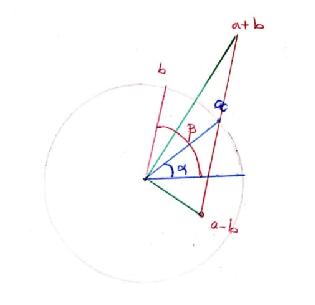
\includegraphics[width=5.29738128033583cm,height=5.12312245834973cm]{figures/Math_oraux-8.pdf}}
\end{center}

Puisque
\[ \frac{\alpha - \left( \frac{\alpha + \beta}{2} \right)}{2} = \frac{\alpha -
   \beta}{4} \not{\in} \pi \mathbb{Z} \]


On a donc $\frac{\alpha - \beta}{4} \in \Theta$.

Ainsi, par r{\'e}currence, pour tous $k, l \in \mathbb{Z}$ et pour tout $n \in
\mathbb{N}^{\ast}$
\[ \frac{k \alpha + l \beta}{2^n} \in \Theta \]


Avec $\alpha \neq 0$ ou $\beta \neq 0$, alors la suite $\left( \frac{k \alpha
+ l \beta}{2^n} \right)_{k, l \in \mathbb{Z}, n \in \mathbb{N}^{\ast}}$est
dense dans $\mathbb{R}$.

Donc, pour tout angle $\gamma$, il existe une suite de vecteurs unitaires qui
converge vers le vecteur unitaire d'angle $\gamma$.

Par fermeture, $T$ contient tous les vecteurs de tous les angles.

Ainsi, $\mathcal{C} \subset T$.

Par suite,
\[ T =\mathcal{C} \]


\tmtextbf{19.} On d{\'e}finie, $\varphi : (x, y) \longmapsto \langle A^{- 1}
x, A^{- 1} y \rangle$, avec $\langle ., . \rangle$ le produit scalaire
associ{\'e} {\`a} $\| . \|_2$.

On a bien que $\varphi$ est d{\'e}finie, et il s'agit bien d'un produit
scalaire.

Il suffit de montrer que pour tout $x \in \mathbb{R}^2$, on a $\varphi (x, x)
= \| x \|^2$ pour conclure.

Notons
\[ \Re = \{ x \in \mathcal{C} | \nobracket  \| A x \| = 1 \} \]


Il s'agit d'une partie ferm{\'e}e de $\mathcal{C}$.

D'apr{\`e}s la question 17, on a $(e_1, e_2) \in \Re$, qui est une base de
$\mathbb{R}^2$, avec $e_1 \not{=} \pm e_2$.

Pour tout $a, b \in \Re$,
\[ \| A (a + b) \|^2 + \| A (a - b) \|^2 \geqslant 4. \]


Avec $a, b \in \mathcal{C}$, alors $\| A (a + b) \|  \leqslant \| a + b \|_2$
et $\| A (a - b) \|  \leqslant \| a - b \|_2$.

Avec
\begin{eqnarray*}
  \| a + b \|^2_2 + \| a - b \|^2_2 & = & 2 (\| a \|^2_2 + \| b \|^2_2)\\
  & = & 4
\end{eqnarray*}
.

Alors,
\[ (\| a + b \|_2^2 - \| A (a + b) \|^2) + (\| a - b \|_2^2 - \| A (a - b)
   \|^2) \leqslant 0 \]


Avec $A \in \mathcal{K}$, donc $\| a + b \|^2 - \| A (a + b) \|^2 \geqslant 0$
et $\| a - b \|^2 - \| A (a - b) \|^2 \geqslant 0$.

Ainsi, $\| a - b \| _2 = \| A (a - b) \| $ et $\| a - b \| _2 = \| A (a - b)
\| $.

Par suite, \ $ \frac{a - b}{\| a - b \| _2} \in \Re$ et $ \frac{a + b}{\| a +
b \| _2} \in \Re$.

Ainsi, d'apr{\`e}s la question pr{\'e}c{\'e}dente, $\Re =\mathcal{C}$.

D'o{\`u}, pour tout $x \in \mathbb{R}^2$,
\[ \| A x \| = \| x \|_2 \]


Par suite,
\begin{eqnarray*}
  \varphi (x, x) & = & \| A^{- 1} x \|_2^2\\
  & = & \| A^{- 1} (A x) \|^2\\
  & = & \| x \|^2
\end{eqnarray*}


D'o{\`u} le r{\'e}sultat.

\

\subsubsection*{4. Alg{\`e}bres valu{\'e}es}

\tmtextbf{20.a.} Soit $x \in A$, alors par d{\'e}finition, il existe $n \in
\mathbb{N}^{\ast}$ et $a_0, \ldots, a_{n - 1} \in \mathbb{R}$ tels que
\[ x^n + a_{n - 1} x^{n - 1} + \cdots + a_1 x + a_0 = 0 \]


Par d{\'e}composition en {\'e}l{\'e}ments simples dans $\mathbb{R}$ du
polyn{\^o}me $X^n + a_{n - 1} X^{n - 1} + \cdots + a_1 X + a_0$. il existe
$b_1, \ldots, b_r, \alpha_1, \ldots, \alpha_l, \beta_1, \ldots, \beta_l \in
\mathbb{R}$ tels que
\[ X^n + a_{n - 1} X^{n - 1} + \cdots + a_1 X + a_0 = \underset{i =
   1}{\overset{r}{\prod}} (X - b_i) \underset{i = 1}{\overset{l}{\prod}} (X^2
   - \alpha_i X - \beta_i) \]


Donc,
\[ \underset{i = 1}{\overset{r}{\prod}} (x - b_i) \underset{i =
   1}{\overset{l}{\prod}} (x^2 - \alpha_i x - \beta_i) = 0 \]


Puisque $A$ est sans diviseur de z{\'e}ro, il existe $i \in \llbracket 1, r
\rrbracket$ tel que $x = b_i$ ou bien il existe $i \in \llbracket 1, l
\rrbracket$ tel que $x^2 = \alpha_i x + \beta_i$.

Dans le premier cas, on a $x^2 = b_i x \in x +\mathbb{R}x$.

Dans le deuxi{\`e}me cas, on a $x^2 \in x +\mathbb{R}x$.

Ainsi, dans tous les cas, $x^2 \in x +\mathbb{R}x$.

D'o{\`u} le r{\'e}sultat.

\

\tmtextbf{20.b.} Puisque $A \neq \mathbb{R}$, il existe $a, b \in \mathbb{R}$
tels que $x^2 = a x + b$ avec $a^2 + 4 b < 0$.

Ainsi,
\begin{eqnarray*}
  \left( x - \frac{a}{2} \right)^2 & = & b + \frac{a^2}{4}\\
  & = & \frac{a^2 + 4 b}{4}
\end{eqnarray*}


On pose
\[ y = \frac{2}{\sqrt{- a^2 - 4 b}} \left( x - \frac{a}{2} \right) \]


On a
\[ \mathbb{R}+\mathbb{R}x =\mathbb{R}+\mathbb{R}y \]


car $(y, 1)$ est $\mathbb{R}$-libre.

D{\'e}finissons $\varphi : a + y b \in \mathbb{R}+\mathbb{R}x \longmapsto a +
i b.$ On a $\varphi$ est bien d{\'e}finie et bijective (par la lib{\'e}rt{\'e}
de $(1, y)$), et de plus, pour tous $a + b y, c + d y \in
\mathbb{R}+\mathbb{R}x$, on a :
\begin{eqnarray*}
  \varphi ((a + b y) + (c + d y)) & = & (a + c) + i (b + d) y\\
  & = & \varphi (c + d y) + \varphi \nobracket (c + d y \nobracket)
\end{eqnarray*}


et
\begin{eqnarray*}
  \varphi ((a + b y) (c + d y)) & = & \varphi (a c + (b c + a d) y - b d )\\
  & = & a c - b d + i (b c + a d)\\
  & = & \varphi (a + b y) \varphi (c + d y)
\end{eqnarray*}


Donc $\varphi$ est un morphisme d'alg{\`e}bre bijectif.

\

\tmtextbf{21.} Montrons qu'il existe $i_A \in A$ tel que $i^2_A = - 1$.

Pour tout $x \in A$, on a $x^2 \in \mathbb{R}+\mathbb{R}x$, donc il existe
$a_x, b_x \in \mathbb{R}$ tels que $x^2 = a_x x + b_x$.

Supposons que pour tout $x \in A$, $a_x^2 + 4 b_x \geqslant 0$.

Alors
\[ \left( x - \frac{a_x - \sqrt{a_x^2 + 4 b_x}}{2} \right) \left( x -
   \frac{a_x + \sqrt{a_x^2 + 4 b_x}}{2} \right) = 0 \]


Or, $A$ est sans diviseur de z{\'e}ro, donc soit $x = \frac{a_x - \sqrt{a_x^2
+ 4 b_x}}{2} \in \mathbb{R}$, soit $x = \frac{a_x + \sqrt{a_x^2 + 4 b_x}}{2}
\in \mathbb{R}$.

Cela implique que $A =\mathbb{R}$, ce qui est absurde.

Ainsi, il existe $x \in \mathbb{R}$ et $a, b \in \mathbb{R}$ tels que $x^2 - a
x - b = 0,$avec $a^2 + 4 b < 0$.

On a alors
\begin{eqnarray*}
  \left( x - \frac{a}{2} \right)^2 & = & b + \frac{a^2}{4}\\
  & = & \frac{a^2 + 4 b}{4}
\end{eqnarray*}


On pose
\[ i_A = \frac{2}{\sqrt{- a^2 - 4 b}} \left( x - \frac{a}{2} \right) \]

On a alors $i^2_A = - 1$.

\

\tmtextbf{22.a.} Soient $x, y \in A$, on a :
\begin{eqnarray*}
  T (x y) & = & i_A x y i_A\\
  & = & - i_A x (i_A i_A) y i_A\\
  & = & - (i_A x i_A) (i_A y i_A)\\
  & = & - T (x) T (y)
\end{eqnarray*}


\tmtextbf{22.b.} On a, pour tout $x \in A$,
\begin{eqnarray*}
  T \circ T (x) & = & i_A (i_A x i_A) i_A\\
  & = & x\\
  & = & \tmop{id} (x)
\end{eqnarray*}


Donc $T \circ T$=id, et ainsi
\[ X^2 - 1 = (X - 1) (X + 1) \]


est un polyn{\^o}me annulateur de $T$. De plus, $X + 1$ et $X - 1$ sont
premiers entre eux. D'apr{\`e}s le th{\'e}or{\`e}me de d{\'e}composition des
noyaux, on a :
\[ A = \ker (T - \tmop{id}) \oplus \ker (T + \tmop{id}) \]

\tmtextbf{23.} Montrons que $\ker (T + \tmop{id}) = U$

Soit $x \in \tmop{Ker} (T + \tmop{id}) \backslash \{ 0 \} \nobracket$. Alors
$T (x) = - x$, donc $x = - i_A x i_A$, ainsi $i_A x = x i_A$.

Donc $x$ et $i_A$ commutent. Par suite,
\[ (i_A x )^2 = - x^2 \]


En particulier, $i_A x \not{\in} \mathbb{R}$, ce qui implique que $(i_A x, 1)$
est une base de $\mathbb{R}+\mathbb{R}x$.

Ainsi, il existe $a, b \in \mathbb{R}$ tels que
\[ x = a + b i_A \in U \]


R{\'e}ciproquement, si $x \in U$, alors il existe $(a, b) \in \mathbb{R}^2$
tel que
\[ x = a + b i_A \]


Donc
\begin{eqnarray*}
  T (x) & = & i_A (a + b  i_A) i_A\\
  & = & i_A a i_A - i_A b\\
  & = & a i_A i_A - b i_A\\
  & = & - a - b i_A\\
  & = & - x
\end{eqnarray*}
Donc
\[ x \in \tmop{Ker} (T + \tmop{id}) \]
Ainsi, $\ker (T + \tmop{id}) = U$, et puisque A n'est pas isomorphe {\`a}
$\mathbb{C}$ et que Ker(T+id) est de dimension 2, alors Ker(T-id) n'est pas
r{\'e}duit {\`a} z{\'e}ro.

\

\tmtextbf{24.} Fixons $\beta \in \tmop{Ker} (T - \tmop{id}) \backslash
\nobracket \{ 0 \}$.

\tmtextbf{24.a.} Montrons que l'application $x \longmapsto \beta x$ envoie
$\ker (T - \tmop{id})$ dans $\ker (T + \tmop{id})$.

Soit $x \in \tmop{Ker} (T - \tmop{id})$, donc $T (x) = x$.

Or, $\beta \in \tmop{Ker} (T - \tmop{id})$, donc $T (\beta) = \beta$.

D'apr{\`e}s la question 22.a, on a :
\begin{eqnarray*}
  T (\beta x) & = & - T (\beta) T (x)\\
  & = & - \beta x
\end{eqnarray*}


Par suite, $\beta x \in \ker (T + \tmop{id})$, donc $x \longmapsto \beta x$
envoie $\ker (T - \tmop{id})$ dans $\ker (T + \tmop{id})$.

D'apr{\`e}s la question pr{\'e}c{\'e}dente, on a $\beta \ker (T - \tmop{id})
\subset U$.

Ainsi, $\dim_{\mathbb{R}} \ker (T - \tmop{id}) \leqslant \dim_{\mathbb{R}} U$

De m{\^e}me $x \longmapsto \beta x$ envoie $\ker (T + \tmop{id})$ dans $\ker
(T - \tmop{id})$, donc $\dim_{\mathbb{R}} (\ker (T - \tmop{id})) \geqslant
\dim_{\mathbb{R}} U$.

On en d{\'e}duit que
\[ \dim_{\mathbb{R}} U = \dim_{\mathbb{R}} \ker (T - \tmop{id}) \]


Par suite, $U = \ker (T - \tmop{id})$.

\

\tmtextbf{24.b.} Montrons que $\beta^2 \in] - \infty, 0 [$.

D'apr{\`e}s ce qui pr{\'e}c{\'e}de, on a $\beta \ker (T - \tmop{id}) \subset
U.$

Donc, $\beta^2 \ker (T - \tmop{id}) \subset \beta U = \ker (T - \tmop{id})$.

Comme $\ker (T - \tmop{id}) \not{=} \{ 0 \}$, il en r{\'e}sulte que $\beta^2
\in \mathbb{R}$.

Supposons par l'absurde que $\beta^2 > 0$. Alors, $\beta = \sqrt{\beta^2} \in
\mathbb{R}$, donc $\beta U = U$.

Ainsi,
\begin{eqnarray*}
  A & = & U + \beta U\\
  & = & U
\end{eqnarray*}


Or, $U$ est isomorphe {\`a} $\mathbb{C}$, ce qui est absurde, car $A$ n'est
pas isomorphe {\`a} $\mathbb{R}$ ni {\`a} $\mathbb{C}$.

D'o{\`u} le r{\'e}sultat.

\

\tmtextbf{24.c.} On a $i_A \in \tmop{Ker} (T + \tmop{id})$, donc $\beta i_A
\in \beta U$. Ainsi, $(\beta, \beta  i_A)$ est une base de $\beta U$, et $(1,
i_A)$ est une base de $U$. Par somme directe, on a $(1, i_A, \beta, \beta
i_A)$ est une base de $A$.

Donc $A$ est isomorphe {\`a} $\mathbb{H}$. (car $\dim_{\mathbb{R}} \mathbb{H}=
4$)

\

\tmtextbf{25.} Soient $x, y \in A$ tels que $x y = y x$ et tels que $V
=\mathbb{R}x +\mathbb{R}y$ soit de dimension 2 sur $\mathbb{R}$.

Montrons que pour tout $u, v \in V$, on a
\[ \| u + v \|^2 + \| u - v \|^2 \geqslant 4 \| u \| . \| v \| \]


Soient $u, v \in \mathbb{R}x +\mathbb{R}y$. Puisque $x, y$ commutent, alors
$u, v$ commutent {\'e}galement, en tant que polyn{\^o}mes $x$et $y$. Or,
\[ \| u + v \|^2 = \| (u + v)^2 \| \infixand \| u - v \|^2 = \| (u - v)^2 \|
\]


Par l'in{\'e}galit{\'e} triangulaire inverse, on a
\begin{eqnarray*}
  \| u + v \|^2 + \| u - v \|^2 & \geqslant & \| (u + v)^2 - (u - v)^2 \|\\
  & \geqslant & 4 \| u \| . \| v \|
\end{eqnarray*}


Montrons que la restriction de $\| . \|$ {\`a} $V$ provient d'un produit
scalaire sur $V$.

On a $V = x\mathbb{R}+ y\mathbb{R}$ de dimension $2$, donc $V$ est isomorphe
{\`a} $\mathbb{R}^2$.

Il existe un isomorphisme d'espaces vectoriels $\varphi : \mathbb{R}^2
\rightarrow V$.

On a, pour tout $x, y \in \mathbb{R}^2$,
\[ \| \varphi (x) + \varphi (y) \|^2 + \| \varphi (x) - \varphi (y) \|^2
   \geqslant 4 \| \varphi (x) \| . \| \varphi (y) \| \]


Ainsi,
\[ \| \varphi (x + y) \|^2 + \| \varphi (x - y) \|^2 \geqslant 4 \| \varphi
   (x) \| . \| \varphi (y) \| \]


Avec $\psi : x \in \mathbb{R}^2 \longmapsto \| \varphi (x) \|$ est une norme
sur $\mathbb{R}^2$, en effet, pour tout $x, y \in \mathbb{R}^2$ et $\lambda
\in \mathbb{R}$, on a

Si $\| \varphi (x) \| = 0$, alors $\varphi (x) = 0$, et par injectivit{\'e},
on a $x = 0$.

De plus, $\| \varphi (\lambda x) \| = | \lambda | \| \varphi (x) \|$ et $\|
\varphi (x + y) \| = \| \varphi (x) + \varphi (y) \| \leqslant \| \varphi (x)
\| + \| \varphi (y) \|$.

D'apr{\`e}s le th{\'e}or{\`e}me $A$, on a $x \longmapsto \| \varphi (x) \|$
provient d'un produit scalaire $\langle . | \nobracket . \rangle$.

Notons
\[ \zeta : (u, v) \in V \longmapsto \langle \varphi^{- 1} (u), \varphi^{- 1}
   (v) \rangle \]
.

On a $\zeta$ est sym{\'e}trique. De plus, pour tout $u \in V$,
\begin{eqnarray*}
  \zeta (u, u) & = & \| \varphi (\varphi^{- 1} (u)) \|\\
  & = & \| u \|\\
  & \geqslant & 0
\end{eqnarray*}


Donc $\zeta$ est positif.

Par lin{\'e}arit{\'e} de $\varphi^{- 1}$, on a $\zeta$ est bilin{\'e}aire.

Et par injectivit{\'e}, $\zeta$ est d{\'e}finie.

Donc $\zeta$ d{\'e}finie un produit scalaire sur $V$.

$\| . \|$ provient de $\zeta$.

D'o{\`u} le r{\'e}sultat.

\

\tmtextbf{26.} Soit $x \in A$. Si $x \in \mathbb{R}$, il est {\'e}vident que
\[ x^2 \in \mathbb{R}+\mathbb{R}x \]


Supposons que $x \in A \backslash \mathbb{R} \nobracket$, alors $V = x
+\mathbb{R}x$ est de dimension 2.

D'apr{\`e}s la question pr{\'e}c{\'e}dente, $\| . \|$ provient d'un produit
scalaire sur $V$.

Notons $y$ un vecteur orthogonal non nul {\`a} $1$ dans $V$.

Ainsi, on a $(1, y)$ forme une base de $V$.

Donc il existe $a, b \in \mathbb{R}$ tels que $x = a + b y$.

Ainsi,
\[ x^2 = a^2 + 2 a b y + y^2 \]


Avec :
\begin{eqnarray*}
  \langle 1, y^2 \rangle & = & \frac{1}{2} (\| y^2 \|^2 + 1 - \| y^2 - 1
  \|^2)\\
  & = & \frac{1}{2} (\| y^2 \|^2 + 1 - \| y  - 1 \|^2 \| y  + 1 \|^2)\\
  & = & \frac{1}{2} (\| y  \|^4 + 1 - (\| y  \|^2 + 1)^2)\\
  & = & \left. \frac{1}{2} (\| y  \|^4 + 1 - \| y  \|^4 - 2 \| y \|^2 - 1
  \nobracket \right)\\
  & = & - \| y^2 \|\\
  & = & - \| 1 \|^2 \| y^2 \|
\end{eqnarray*}


Et donc, d'apr{\`e}s le cas d'{\'e}galit{\'e} dans l'in{\'e}galit{\'e} de
Cauchy-Schwarz, on a $y^2 \in \mathbb{R}$.

D'o{\`u} :
\begin{eqnarray*}
  x^2 & \in & \mathbb{R}+\mathbb{R}_y\\
  & = & \mathbb{R}+\mathbb{R}_x
\end{eqnarray*}


27. D'apr{\`e}s la question pr{\'e}c{\'e}dente, on a A est alg{\'e}brique (car
Pour tout $x \in \mathbb{R}$, il existe $a, b \in \mathbb{R}$ tels que $x^2 = ax + b$).

De plus, A est sans diviseur de z{\'e}ro : en effet, pour $x, y \in A$ tels
que $x y = 0,$ on alors

$\|x\|\|y\|=\|x y\|= 0$

\ \ \ \ \

Par cons{\'e}quent $\|x\|= 0$ ou $\|y\|= 0.$

Par suite $x = 0$ou $y = 0$.

Ainsi, d'apr{\`e}s le th{\'e}or{\`e}me $B$, $A$ est isomorphe {\`a}
\ensuremath{\mathbb{R}}, \ensuremath{\mathbb{C}} ou \ensuremath{\mathbb{H}}.

D'o{\`u} le th{\'e}or{\`e}me $C$.
\newpage
\begin{center}
\textbf{ÉCOLES NORMALES SUPÉRIEURES}\\
\textbf{CONCOURS D'ADMISSION 2018\hspace{11em}FILIÈRE MPI}\\
\subsection*{Composition de mathématiques - C - (ULCR)}\label{mathC_2018}
\textbf{Corrigé par : SABIR ILYASS.}
\end{center}
\[
\star \star \star
\]
\addcontentsline{toc}{subsection}{Composition de mathématiques - C - MPI - 2018}

\begin{center}
  {\tmname{Partie I}}
\end{center}

Dans cette partie, $E$ est un ensemble fini ou d{\'e}nombrable. L'ensemble des
probabilit{\'e}s sur $E$ est l'ensemble
\[ \mathcal{P} (E) = \left\{ \mu : E \rightarrow [0, 1]  | \nobracket 
   \underset{x \in E}{\sum} \mu (x) = 1 \right\} \]


Une matrice de transition sur $E$ est une application $P : E \times E
\rightarrow [0, 1]$ telle que, pour tout $x \in E$, on a
\[ \underset{y \in E}{\sum} P (x, y) = 1 \]


Le produit $P Q$de deux matrices de transition $P$ et $Q$ est d{\'e}fini par
\[ \forall (x, z) \in E \times E, (P Q) (x, z) = \underset{y \in E}{\sum} P
   (x, y) Q (y, z) \]


On notera $I$ la matrice de transition d{\'e}finie par
\[ I (x, y) = \left\{\begin{array}{l}
     1 \tmop{si} x = y\\
     0 \tmop{si} x \not{=} y
   \end{array}\right. \]


\textbf{1.1.} (a) \textbf{Vérifier que si $P$ et $Q$ sont des matrices de transition, alors $PQ$ est aussi une matrice de transition.}


Soient $P, Q$ deux matrices de transition, on a pour tout $x \in E$
\begin{eqnarray*}
  \underset{y \in E}{\sum} (P Q) (x, y) & = & \underset{y \in E}{\sum}
  \underset{z \in E}{\sum} P (x, z) Q (z, y)
\end{eqnarray*}


Avec, la famille $(P (x, z) Q (z, y))_{(y, z) \in E \times E}$ est {\`a}
termes positifs, donc via le th{\'e}or{\`e}me de Fubini-Tonelli on a :
\begin{eqnarray*}
  \underset{y \in E}{\sum} (P Q) (x, y) & = & \underset{z \in E}{\sum}
  \underset{y \in E}{\sum} P (x, z) Q (z, y)\\
  & = & \underset{z \in E}{\sum} P (x, z) \underset{y \in E}{\sum} Q (z, y)
\end{eqnarray*}


Puisque $Q$ est une matrice de transition, alors $\underset{y \in E}{\sum} Q
(z, y) = 1$,

Ensuite, $\underset{y \in E}{\sum} (P Q) (x, y) = \underset{z \in E}{\sum} P
(x, z) = 1$, car $P$ est une matrice de transition, d'o{\`u} le r{\'e}sultat.

\

\qquad (b) \textbf{Vérifier que si $P$, $Q$ et $R$ sont des matrices de transition, on a $(PQ)R = P(QR)$.}


Pour tout $(x, y) \in E \times E$. On a
\begin{eqnarray*}
  (P Q) R (x, y) & = & \underset{z \in E}{\sum} (P Q) (x, z) R (z, y)\\
  & = & \underset{z \in E}{\sum} \underset{t \in E}{\sum} P (x, t) Q (t, z) R
  (z, y)
\end{eqnarray*}


La famille $(P (x, t) Q (t, z) R (z, y))_{(z, t) \in E \times E}$ est {\`a}
termes positifs, donc d'apr{\`e}s le th{\'e}or{\`e}me de Fubini-Tonelli, on
peut permuter les sommes. Ainsi, on a :
\begin{eqnarray*}
  (P Q) R (x, y) & = & \underset{t \in E}{\sum} \underset{z \in E}{\sum} P (x,
  t) Q (t, z) R (z, y)\\
  & = & \underset{t \in E}{\sum} P (x, t) \underset{z \in E}{\sum} Q (t, z) R
  (z, y)\\
  & = & \underset{t \in E}{\sum} P (x, t) (\tmop{QR}) (t, y)\\
  & = & P (Q R) (x, y)
\end{eqnarray*}


Et ceci est vrai pour tout $(x, y) \in E \times E$, donc $(P Q) R = P (Q R)$.

\

\qquad$(c)$ Pour tout entier $n \geqslant 0$ et toute matrice de transition
$P$, on d{\'e}finit $P^n$ par $P^0 = I$ et la relation de r{\'e}currence $P^{n
+ 1} = P^n P$ si $n \geqslant 0$. \tmtextbf{V{\'e}rifier que $P^n$ est bien
une matrice de transition.}

Par r{\'e}currence sur $n \in \mathbb{N}$, on a pour $n = 0$, $P^0 = I$, qui
est bien une matrice de transition.

Soit $n \in \mathbb{N}.$ Supposons que $P^n $est une matrice de transition.
Puisque $P$est une matrice de transition, alors d'apr{\`e}s la
question\tmtextbf{ 1.1.a}, le produit $P^{n + 1} = P^n P$ est une matrice de
transition,

D'o{\`u} le r{\'e}sultat.

\

{\'E}tant donn{\'e}s $\mu \in \mathcal{P}(E)$, une matrice de transition$P$,
et des fonctions born{\'e}es $f : E \rightarrow \mathbb{R}$ et$g : E
\rightarrow \mathbb{R}$, on d{\'e}finit les nombres r{\'e}els suivants
\begin{eqnarray*}
  \mu [f] & = & \underset{x \in E}{\sum} \mu (x) f (x) .\\
  \mu P (y) & = & \underset{x \in E}{\sum} \mu (x) P (x, y), o{\`u} y \in E.\\
  P f (x) & = & \underset{y \in E}{\sum} P (x, y) f (y), o{\`u} x \in E.\\
  \langle f, g \rangle_{\mu} & = & \mu [f g] .
\end{eqnarray*}


\textbf{1.2.} Soit $\mu \in \mathcal{P}(E)$, soient $P$ et $Q$ des matrices
de transition et soit $f : E \rightarrow \mathbb{R}$ une fonction born{\'e}e.

\textbf{$(a$) Montrer que $\mu P \in \mathcal{P}(E)$ et que $(\mu P) Q
= \mu (P Q)$.}

Montrons d'abord que $\mu P \in \mathcal{P} (E)$.

On a, pour tout $x \in E$
\begin{eqnarray*}
  \underset{x \in E}{\sum} \mu P (x) & = & \underset{x \in E}{\sum}
  \underset{y \in E}{\sum} \mu (y) P (y, x)
\end{eqnarray*}


La famille $(\mu (y) P (y, x))_{(x, y) \in E \times E}$ est {\`a} termes
positifs, donc via le th{\'e}or{\`e}me de Fubini-Tonelli, on a :
\begin{eqnarray*}
  \underset{x \in E}{\sum} \mu P (x) & = & \underset{y \in E}{\sum}
  \underset{x \in E}{\sum} \mu (y) P (y, x)\\
  & = & \underset{y \in E}{\sum} \mu (y) \left( \underset{x \in E}{\sum} P
  (y, x) \right) \tmmathbf{}\\
  & = & \underset{y \in E}{\sum} \mu (y)  (\tmop{car} P \tmop{est} \tmop{une}
  \tmop{matrice} \tmop{de} \tmop{transition})\\
  & = & 1 (\tmop{car} \mu \in \mathcal{P} (E))
\end{eqnarray*}


De plus, pour tout $x \in E$, on a
\[ 0 \leqslant \mu P (x) \leqslant \underset{x \in E}{\sum} \mu P (x) = 1 \]


Donc, $\mu P \in \mathcal{P}(E)$.

Montrons maintenant que $(\mu P) Q = \mu (P Q)$.

On a, pour tout $y \in E$,
\begin{eqnarray*}
  (\mu P) Q (x) & = & \underset{x \in E}{\sum} (\mu P) (x) Q (x, y)\\
  & = & \underset{x \in E}{\sum} \underset{z \in E}{\sum} \mu (z) P (z, x) Q
  (x, y)
\end{eqnarray*}


Avec la famille $(\mu (z) P (z, x) Q (x, y))_{(x, z) \in E \times E}$ est
{\`a} termes positifs, donc, via le th{\'e}or{\`e}me de Fubini-Tonelli, on a :
\begin{eqnarray*}
  (\mu P) Q (x) & = & \underset{z \in E}{\sum} \underset{x \in E}{\sum} \mu
  (z) P (z, x) Q (x, y)\\
  & = & \underset{z \in E}{\sum} \mu (z) \left( \underset{x \in E}{\sum} P
  (z, x) Q (x, y) \right)\\
  & = & \underset{z \in E}{\sum} \mu (z) (P Q) (z, y)\\
  & = & \mu (P Q) (y)
\end{eqnarray*}


D'o{\`u} le r{\'e}sultat.

\

\textbf{$(b)$ Montrer que $P f : E \rightarrow \mathbb{R}$ est une
fonction born{\'e}e et que $\mu P [f] = \mu [P f] .$}

On a pour tout $x \in E$ :
\begin{eqnarray*}
  | P f (x) | & = & \left| \underset{y \in E}{\sum} P (x, y) f (y) \right|\\
  & \leqslant & \underset{y \in E}{\sum} P (x, y) | f (y) |\\
  & \leqslant & \underset{z \in E}{\max} | f (z) | \underset{y \in E}{\sum} P
  (x, y)\\
  & \leqslant & \underset{z \in E}{\max} | f (z) |\\
  & < & + \infty \quad  (\tmop{car} f \tmop{est} \tmop{born} {\'e}e)
\end{eqnarray*}


D'o{\`u} $P f$ est born{\'e}e. Montrons maintenant que $\mu P [f] = \mu [P f]$

On a
\begin{eqnarray*}
  \mu P [f] & = & \underset{x \in E}{\sum} \mu P (x) f (x)\\
  & = & \underset{x \in E}{\sum} \underset{y \in E}{\sum} \mu (y) P (y, x) f
  (x)
\end{eqnarray*}


La famille $(\mu (y) P (y, x) f (x))_{(x, y) \in E \times E}$ est sommable, en
effet, on a
\begin{eqnarray*}
  \underset{y \in E}{\sum} \underset{x \in E}{\sum} | \mu (y) P (y, x) f (x) |
  & = & \underset{y \in E}{\sum} \mu (y) \underset{x \in E}{\sum} P (y, x) | f
  (x) |\\
  & \leqslant & \| f \|_{\infty} \underset{y \in E}{\sum} \mu (y) \underset{x
  \in E}{\sum} P (y, x)\\
  & = & \| f \|_{\infty} \underset{y \in E}{\sum} \mu (y)\\
  & = & \| f \|_{\infty}\\
  & < & + \infty
\end{eqnarray*}


Donc, d'apr{\`e}s le th{\'e}or{\`e}me de Fubini-Tonelli, la famille $(\mu (y)
P (y, x) f (x))_{(x, y) \in E \times E}$ est sommable.

Et on a
\begin{eqnarray*}
  \mu P [f] & = & \underset{x \in E}{\sum} \underset{y \in E}{\sum} \mu (y) P
  (y, x) f (x)\\
  & = & \underset{y \in E}{\sum} \mu (y) \left( \underset{x \in E}{\sum} P
  (y, x) f (x) \right)\\
  & = & \underset{y \in E}{\sum} \mu (y) P f (y)\\
  & = & \mu [P f]
\end{eqnarray*}


\tmtextbf{\qquad$(c)$Montrer que $(P Q) f = P (Q f)$.}

Pour tout $x \in E$, on a
\begin{eqnarray*}
  (P Q) f (x) & = & \underset{y \in E}{\sum} (P Q) (x, y) f (y)\\
  & = & \underset{y \in E}{\sum} \underset{z \in E}{\sum} P (x, z) Q (z, y) f
  (y)
\end{eqnarray*}


La famille $(P (x, z) Q (z, y) f (y))_{(y, z) \in E \times E}$ est sommable,
en effet
\begin{eqnarray*}
  \underset{z \in E}{\sum} \underset{y \in E}{\sum} | P (x, z) Q (z, y) f (y)
  | & = & \underset{z \in E}{\sum} \underset{y \in E}{\sum} P (x, z) Q (z, y)
  | f (y) |\\
  & \leqslant & \| f \|_{\infty} \underset{z \in E}{\sum} P (x, z) \left(
  \underset{y \in E}{\sum} Q (z, y) \right)\\
  & = & \| f \|_{\infty} \underset{z \in E}{\sum} P (x, z)\\
  & = & \| f \|_{\infty}\\
  & < & + \infty
\end{eqnarray*}


Et donc, via le th{\`e}or{\'e}me de Fubini-Tonelli, on a
\begin{eqnarray*}
  (P Q) f (x) & = & \underset{z \in E}{\sum} \underset{y \in E}{\sum} P (x, z)
  Q (z, y) f (y)\\
  & = & \underset{z \in E}{\sum} P (x, z) \left( \underset{y \in E}{\sum} Q
  (z, y) f (y) \right)\\
  & = & \underset{z \in E}{\sum} P (x, z) (Q f) (z)\\
  & = & P (Q f) (x)
\end{eqnarray*}


Et cela pour tout $x \in E$. D'o{\`u} $(P Q) f = P (Q f)$.

\

Une matrice de transition $P$ est dite \tmtextbf{r{\'e}versible} par rapport
{\`a} un {\'e}l{\'e}ment $\pi$ de $\mathcal{P}(E)$ si pour tout $(x, y) \in
E^2$ , on a
\[ \pi (x) P (x, y) = \pi (y) P (y, x) . \]


Une matrice de transition $P$ est dite\tmtextbf{ irr{\'e}ductible} si, pour
tout $(x, y) \in E^2$ , il existe un entier $n \geqslant 1$ tel que $P^n (x,
y) > 0$.

On se donne, sur un espace probabilis{\'e} $({\textohm}, \mathcal{A},
\mathbb{P})$, une suite ($U_n)_{n \geqslant 1}$ de variables al{\'e}atoires
r{\'e}elles ind{\'e}pendantes et identiquement distribu{\'e}es, et une
variable al{\'e}atoire$X_0$ {\`a} valeurs dans $E$, ind{\'e}pendante de la
suite ($U_n)_{n \geqslant 1}$. On se donne une fonction $F : E \times
\mathbb{R} \rightarrow E$ et on d{\'e}finit une suite $(X_n)_{n \geqslant 1}$
de variables al{\'e}atoires {\`a} valeurs dans $E$ en posant, pour tout entier
$n \geqslant 1$,
\[ X_n = F (X_{n - 1}, U_n) \]


La loi de $X_n$ est not{\'e}e$\mu_n$. On rappelle que c'est l'{\'e}l{\'e}ment
de $\mathcal{P}(E)$ d{\'e}fini par $\mu_n (x) =\mathbb{P}[X_n = x]$ pour tout
$x \in E$.

L'esp{\'e}rance d'une variable al{\'e}atoire r{\'e}elle born{\'e}e $X$ sera
not{\'e}e $\mathbb{E}[X]$.

Pour tout $(x, y) \in E^2$, on pose $P (x, y) =\mathbb{P}[F (x, U_1) = y]$.

\

\textbf{1.3. (a) Vérifier que $P$ est une matrice de transition et que, pour tout entier $n \geqslant 0$ et tout $(x_0, \ldots, x_n) \in E^{n+1}$, on a }
\[
\mathbb{P}[X_0 = x_0, \ldots, X_n = x_n] = \mu_0(x_0) \prod_{i=1}^{n} P(x_{i-1}, x_i).
\]


\

V{\'e}rifiant d'abord que $P$ est une matrice de transition. On a pour tout
$x \in E$:
\begin{eqnarray*}
  \underset{y \in E}{\sum} P (x, y) & = & \underset{y \in E}{\sum}
  \mathbb{P}[F (x, U_1) = y]\\
  & = & 1
\end{eqnarray*}


D'o{\`u} $P$ est une matrice de transition.

On a pour tout $n \in \mathbb{N}$
\begin{eqnarray*}
  \mathbb{P}[X_0 = x_0, . . ., X_n = x_n] & = & \mathbb{P}[X_0 = x_0, . . .,
  X_{n - 1} = x_{n - 1}, X_n = x_n]\\
  & = & \mathbb{P}[X_0 = x_0, . . ., X_{n - 1} = x_{n - 1}, F (X_{n - 1},
  U_n) = x_n]\\
  & = & \mathbb{P}[X_0 = x_0, . . ., X_{n - 1} = x_{n - 1}, F (x_{n - 1},
  U_n) = x_n]
\end{eqnarray*}


Par it{\'e}ration, on obtient
\begin{eqnarray*}
  \mathbb{P}[X_0 = x_0, . . ., X_n = x_n] & = & \mathbb{P}[X_0 = x_0, F (x_0,
  U_n) = x_1 . . .,, F (x_{n - 1}, U_n) = x_n]
\end{eqnarray*}


Avec ($U_n)_{n \geqslant 1}$ est une suite de variables al{\'e}atoires
r{\'e}elles ind{\'e}pendantes et identiquement distribu{\'e}es, alors pour
tout $x \in \mathbb{R}$, $(F (x , U_k))_{k \geqslant 1}$ est une suite de
variables al{\'e}atoires ind{\'e}pendantes et identiquement distribu{\'e}es.
Par ailleurs, $X_0$ est ind{\'e}pendante de la suite ($U_n)_{n \geqslant 1}$.
Ainsi, $X_0 $est {\'e}galement ind{\'e}pendante de la suite $(F (x , U_k))_{k
\geqslant 1}$, o{\`u} $x \in E$.

On a alors
\begin{eqnarray*}
  \mathbb{P}[X_0 = x_0, . . ., X_n = x_n] & = & \mathbb{P}[X_0 = x_0]
  \underset{k = 1}{\overset{n}{\prod}} \mathbb{P} [F (x_{k - 1}, U_n) = x_k]\\
  & = & \mathbb{P}[X_0 = x_0] \underset{k = 1}{\overset{n}{\prod}} \mathbb{P}
  [F (x_{k - 1}, U_1) = x_k]\\
  & = & \mu_0 (x_0) \underset{k = 1}{\overset{n}{\prod}} P (x_{k - 1}, x_k)
\end{eqnarray*}


\textbf{$(b)$Montrer que pour tout entier $n \geqslant 0$ et tout
$(x_0, . . ., x_n) \in E^{n + 1}$ tel que $\mathbb{P}[X_0 = x_0, . . ., X_n =
x_n] > 0$, on a, pour tout $x \in E,$}

\[ \mathbb{P}[X_{n + 1} = x | \nobracket X_0 = x_0, . . ., X_n = x_n] = P (x_n, x) \]

Soit $n \in \mathbb{N}$, $x \in E$ et soit $(x_0, . . ., x_n) \in E^{n + 1}$
tel que $\mathbb{P}[X_0 = x_0, . . ., X_n = x_n] > 0$.

Posons $x_{n + 1} = x$. En utilisant la question pr{\'e}c{\'e}dente, on a
\begin{eqnarray*}
  \mathbb{P}[X_{n + 1} = x_{n + 1} | \nobracket X_0 = x_0, . . ., X_n = x_n] &
  = & \frac{\mathbb{P}[X_0 = x_0, . . ., X_n = x_n, X_{n + 1} = x_{n +
  1}]}{\mathbb{P}[X_0 = x_0, . . ., X_n = x_n]}\\
  & = & \frac{\mu_0 (x_0) \underset{k = 1}{\overset{n + 1}{\prod}} P (x_{k -
  1}, x_k)}{\mu_0 (x_0) \underset{k = 1}{\overset{n}{\prod}} P (x_{k - 1},
  x_k)}\\
  & = & P (x_n, x_{n + 1})\\
  & = & P (x_n, x)
\end{eqnarray*}


D'o{\`u} le r{\'e}sultat.

\

\textbf{$(c)$Montrer que pour tout$n \geqslant 0,$ on a $\mu_n =
\mu_0 P^n$ et que si $\mu_0 P = \mu_0,$ alors $\mu_n = \mu_0$ pour tout $n
\geqslant 0$.}

Soit $n \in \mathbb{N}$, pour tout $x \in E$, on a, par formule de
probabilit{\'e} totale, en utilisant la question 1.3.a, et en posant $x_n = x$
:
\begin{eqnarray*}
  \mu_n (x) & = & \mathbb{P}[X_n = x]\\
  & = & \underset{x_0 \in E}{\sum} \underset{x_1 \in E}{\sum} \ldots
  \underset{x_{n - 1} \in E}{\sum} \mathbb{P}[X_n = x, X_0 = x_0, . . ., X_{n
  - 1} = x_{n - 1}]\\
  & = & \underset{x_0 \in E}{\sum} \underset{x_1 \in E}{\sum} \ldots
  \underset{x_{n - 1} \in E}{\sum} \mathbb{P}[X_0 = x_0, . . ., X_{n - 1} =
  x_{n - 1}, X_n = x]\\
  & = & \underset{x_0 \in E}{\sum} \underset{x_1 \in E}{\sum} \ldots
  \underset{x_{n - 1} \in E}{\sum} \mu_0 (x_0) \underset{k =
  1}{\overset{n}{\prod}} P (x_{k - 1}, x_k)\\
  & = & \underset{x_0 \in E}{\sum} \mu_0 (x_0) \underset{x_1 \in E}{\sum}
  \ldots \underset{x_{n - 1} \in E}{\sum} \underset{k = 1}{\overset{n}{\prod}}
  P (x_{k - 1}, x_k)
\end{eqnarray*}


Par une simple r{\'e}currence, on peut montrer la formule qui donne le produit
fini de plusieurs matrices de transitions :
\[ \underset{x_1 \in E}{\sum} \ldots \underset{x_{n - 1} \in E}{\sum}
   \underset{k = 1}{\overset{n}{\prod}} P (x_{k - 1}, x_k) = P^n (x_0, x_n) \]


D'o{\`u}
\begin{eqnarray*}
  \mu_n (x) & = & \underset{x_0 \in E}{\sum} \mu_0 (x_0) P^n (x_0, x_n)\\
  & = & \mu_0 P^n (x_n)\\
  & = & \mu_0 P^n (x )
\end{eqnarray*}


Et {\c c}a pour tout $x \in E$, alors
\[ \mu_n = \mu_0 P^n \]


Supposons maintenant que $\mu_0 P = \mu_0,$ Et montrons par r{\'e}currence que
$\mu_n = \mu_0$ pour tout $n \geqslant 0$.

Pour $n = 0$, on a bien $\mu_0 P^0 = \mu_0 I = \mu_0$.

Soit $n \in \mathbb{N}$, supposons que $\mu_n = \mu_0 P^n$, et montrons que
$\mu_n = \mu_0 P^{n + 1}$.

On a par hypoth{\`e}se de r{\'e}currence
\[ \mu_n P^{n + 1} = (\mu_0 P^n) P = \mu_0 P = \mu_0  \]


D'o{\`u} le r{\'e}sultat.

\

\tmtextbf{$(d)$ Montrer que pour tout $n \geqslant 0$ et tout $x \in E$ tel que $\mu_0 (x) > 0$, on a }
\[ \mathbb{P}[X_n = y | X_0 = x] = P^n (x, y) \tmop{pour} \tmop{tout} y \in E.
\]

\

Soit $n \in \mathbb{N}$. On a, pour tout $x, y \in E$, tel que $\mu_0 (x) >
0$
\begin{eqnarray*}
  \mathbb{P}[X_n = y | X_0 = x] & = & \frac{\mathbb{P}[X_n = y, X_0 =
  x]}{\mathbb{P}[X_0 = x]}\\
  & = & \frac{1}{\mu_0 (x)} \mathbb{P}[X_n = y, X_0 = x]
\end{eqnarray*}


Notons $x_0 = x$, et $x_n = y$. On a alors :
\begin{eqnarray*}
  \mathbb{P}[X_n = y | X_0 = x] & = & \frac{1}{\mu_0 (x)} \underset{x_1 \in
  E}{\sum} \ldots \underset{x_{n - 1} \in E}{\sum} \mathbb{P}[X_0 = x_0, . .
  ., X_{n - 1} = x_{n - 1}, X_n = x]\\
  & = & \frac{1}{\mu_0 (x)} \underset{x_1 \in E}{\sum} \ldots \underset{x_{n
  - 1} \in E}{\sum} \mu_0 (x_0) \underset{k = 1}{\overset{n}{\prod}} P (x_{k -
  1}, x_k)\\
  & = & \underset{x_1 \in E}{\sum} \ldots \underset{x_{n - 1} \in E}{\sum}
  \underset{k = 1}{\overset{n}{\prod}} P (x_{k - 1}, x_k)\\
  & = & P^n (x_0, x_n)\\
  & = & P^n (x, y)
\end{eqnarray*}


D'o{\`u} le r{\'e}sultat.

\

\tmtextbf{$(e)$ Montrer que pour toute fonction$f : E \rightarrow \mathbb{R}$ born{\'e}e, on a}
\[ \mathbb{E} [f (X_n)] = \mu_0 [P^n f] . \]

\

On a
\begin{eqnarray*}
  \mathbb{E} [f (X_n)] & = & \underset{x \in E}{\sum} f (x) \mathbb{P} [X_n =
  x]\\
  & = & \underset{x \in E}{\sum} f (x) \mu_n (x)\\
  & = & \underset{x \in E}{\sum} \mu_0 P^n (x) f (x)\\
  & = & \mu_0 P^n [f]\\
  & = & \mu_0 [P^n f] \quad  (d' \tmop{apr} {\`e}s \tmop{la} \tmop{question}
  1.2. c)
\end{eqnarray*}


{\`A} partir de maintenant, on supposera que

$\bullet$ $P$ est r{\'e}versible par rapport {\`a} une probabilit{\'e} $\pi
\in \mathcal{P}(E)$,

$\bullet$ il existe $a \in E$ tel que $\pi (a) > 0$ et tel que, pour tout $x
\in E$, il existe un entier$n \geqslant 1$ pour lequel $P^n (a, x) > 0.$

\

\textbf{1.4. Montrer que $\pi P = \pi$.}

On a, pour tout $x \in E$
\begin{eqnarray*}
  \pi P (x) & = & \underset{y \in E}{\sum} \pi (y) P (y, x)\\
  & = & \underset{y \in E}{\sum} \pi (x) P (x, y)\\
  & = & \pi (x) \underset{y \in E}{\sum} P (x, y)\\
  & = & \pi (x)
\end{eqnarray*}


Et {\c c}a pour tout $x \in E$, alors $\pi P = \pi$.

\

\textbf{1.5. $(a)$ Montrer que pour tout $n \geqslant 1$, la matrice
de transition $P^n $est r{\'e}versible par rapport {\`a} $\pi$.}

Essayons de montrer le r{\'e}sultat par r{\'e}currence sur $n \in
\mathbb{N}^{\ast}$.

Pour $n = 1$, par d{\'e}finition de $P$, $P$ est r{\'e}versible par rapport
{\`a} $\pi$.

Soit $n \in \mathbb{N}^{\ast}$. Supposons que $P^n $est r{\'e}versible par
rapport {\`a} $\pi$, et montrons que $P^{n + 1} $est r{\'e}versible par
rapport {\`a}$\pi$.

On a
\begin{eqnarray*}
  \pi (x) P^{n + 1} (x, y) & = & \pi (x) (P^n P) (x, y)\\
  & = & \underset{z \in E}{\sum} \pi (x) P^n (x, z) P (z, y)\\
  & = & \underset{z \in E}{\sum} \pi (z) P^n (z, x) P (z, y)\\
  & = & \underset{z \in E}{\sum} \pi (z) P (z, y) P^n (z, x)\\
  & = & \underset{z \in E}{\sum} \pi (y) P (y, z) P^n (z, x)\\
  & = & \pi (y) \underset{z \in E}{\sum} P (y, z) P^n (z, x)\\
  & = & \pi (y) (P P^n) (y, x)\\
  & = & \pi (y) P^{n + 1} (y, x)
\end{eqnarray*}


Ainsi \ $P^{n + 1} $est r{\'e}versible par rapport {\`a}$\pi$, d'o{\`u} le
r{\'e}sultat par r{\'e}currence sur $n \geqslant 1$.

\

\textbf{$(b)$Soit$n \geqslant 1$ et soit $x \in E$. Montrer que si
$P^n (a, x) > 0$, alors $P^n (x, a) > 0$et $\pi (x) > 0.$}

D'apr{\`e}s la question pr{\'e}c{\'e}dente, on a
\[ \pi (a) P^n (a, x) = \pi (x) P^n (x, a) \]


Puisque $\pi (a) > 0$, et $P^n (a, x) > 0$, on en d{\'e}duit que $\pi (x) P^n
(x, a) > 0$.

Comme $\pi (x) \geqslant 0$, on obtient alors $P^n (x, a) > 0$et $\pi (x) >
0.$

\

\textbf{(c) Montrer que $\pi (x) > 0$ pour tout $x \in E$. }

On a pour tout $x \in E$, il existe un entier$n \geqslant 1$ pour lequel $P^n
(a, x) > 0.$ D'apr{\`e}s la question pr{\'e}c{\'e}dente, on en conclut que
$\pi (x) > 0$.

\

\textbf{(d) Montrer que $P$ est irr{\'e}ductible.}

Soit $(x, y) \in E^2$, il existe $n_1, n_2 > 0$ tels que $P^{n_1} (a, x) > 0$
et $P^{n_2} (a, y) > 0$.

D'apr{\`e}s la question pr{\'e}c{\'e}dente, on a $\pi (x) > 0$, $\pi (y) > 0$.
On en d{\'e}duit que :
\begin{eqnarray*}
  P^{n_1 + n_2} (x, y) & = & (P^{n_1} \times P^{n_2}) (x, y)\\
  & = & \underset{z \in E}{\sum} P^{n_1} (x, z) P^{n_2} (z, x)\\
  & \geqslant & P^{n_1} (x, a) P^{n_2} (a, x)
\end{eqnarray*}


Or, d'apr{\`e}s la question 1.5.a, $P^{n_1}$ est r{\'e}versible par rapport
{\`a}$\pi$. Ainsi


\begin{eqnarray*}
  P^{n_1} (x, a) & = & \frac{\pi (a)}{\pi (x)} P^{n_1} (a, x) > 0
\end{eqnarray*}


Par cons{\'e}quent, $P^{n_1 + n_2} (x, y) > 0$, pour tout $(x, y) \in E^2$, et
donc, par d{\'e}finition, $P$ est irr{\'e}ductible.

\

\tmtextbf{1.6.} Pour toute fonction $f : E \rightarrow \mathbb{R}$ born{\'e}e
et tout entier $n \geqslant 1$, on pose
\[ \mathcal{E}_n (f) = \frac{1}{2} \underset{(x, y) \in E^2}{\sum}  [f (x) - f
   (y)]^2 \pi (x) P^n (x, y) \]


{\hspace{3em}}\tmtextbf{(a) Montrer que $\mathcal{E}_n (f) = \langle f - P^n
f, f \rangle_{\pi}$.}

On a
\begin{eqnarray*}
  \langle f - P^n f, f \rangle_{\pi} & = & \pi [(f - P^n f) f]\\
  & = & \underset{x \in E}{\sum} \pi (x) (f (x) - P^n f (x)) f (x)\\
  & = & \underset{x \in E}{\sum} \pi (x) \left( f (x) - \underset{y \in
  E}{\sum} P^n (x, y) f (y) \right) f (x)
\end{eqnarray*}


Montrons que la famille ${(\pi (x) (f (x) - f (y)) f (x) P^n (x, y))_{(x, y)
\in E^2}} $ est sommable.

Puisque $P$ est r{\'e}versible par rapport {\`a} $\pi$, on a:
\begin{eqnarray*}
  \underset{(x, y) \in E^2}{\sum} | \pi (x) (f (x) - f (y)) f (x) P^n (x, y) |
  & = & \underset{(x, y) \in E^2}{\sum} | \pi (y) (f (y) - f (x)) f (y) P^n
  (y, x) |\\
  & = & \underset{y \in E}{\sum} \pi (y) | f (y) | \underset{x \in E}{\sum} |
  f (y) - f (x) | P^n (y, x)\\
  & \leqslant & 2 \| f \|_{\infty} \underset{y \in E}{\sum} \pi (y) | f (y) |
  \underset{x \in E}{\sum} P^n (y, x)\\
  & = & 2 \| f \|_{\infty} \underset{y \in E}{\sum} \pi (y) | f (y) |
\end{eqnarray*}


Car $\underset{x \in E}{\sum} P^n (y, x) = 1$, pour tout $y \in E$, puisque
$P^n $est une matrice de transition.

On a alors
\begin{eqnarray*}
  \underset{(x, y) \in E^2}{\sum} | \pi (x) (f (x) - f (y)) f (x) P^n (x, y) |
  & \leqslant & 2 \| f \|^2_{\infty} \underset{y \in E}{\sum} \pi (y)\\
  & = & 2 \| f \|^2_{\infty}\\
  & < & + \infty
\end{eqnarray*}


Donc, la famille ${(\pi (x) (f (x) - f (y)) f (x) P^n (x, y))_{(x, y) \in
E^2}} $ est sommable, et on a
\begin{eqnarray*}
  \langle f - P^n f, f \rangle_{\pi} & = & \underset{x \in E }{\sum} \pi (x)
  \left( f (x) \underset{y \in E}{\sum} P^n (x, y) - \underset{y \in E}{\sum}
  P^n (x, y) f (y) \right) f (x) \qquad (\ast)\\
  & = & \underset{(x, y) \in E^2}{\sum} \pi (x) (f (x) - f (y)) f (x) P^n (x,
  y)
\end{eqnarray*}


Et puisque $P$ est r{\'e}versible par rapport {\`a} $\pi,$ alors
\begin{eqnarray*}
  \underset{(x, y) \in E^2}{\sum} \pi (x) (f (x) - f (y)) f (x) P^n (x, y) & =
  & \underset{(x, y) \in E^2}{\sum} \pi (y) (f (y) - f (x)) f (y) P^n (y, x)\\
  & = & \underset{(x, y) \in E^2}{\sum} \pi (x) (f (y) - f (x)) f (y) P^n (x,
  y)
\end{eqnarray*}

Ainsi,
\begin{eqnarray*}
  \underset{(x, y) \in E^2}{\sum} \pi (x) (f (x) - f (y)) f (x) P^n (x, y) & =
  & \frac{1}{2} \underset{(x, y) \in E^2}{\sum} \pi (x) (f (x) - f (y)) f (x)
  P^n (x, y)\\
  &  & + \frac{1}{2} \underset{(x, y) \in E^2}{\sum} \pi (x) (f (y) - f (x))
  f (y) P^n (x, y)\\
  & = & \frac{1}{2} \underset{(x, y) \in E^2}{\sum} \pi (x) (f (x)^2 - 2 f
  (y) \nobracket f (x) + \nobracket f (y)^2) P^n (x, y)\\
  & = & \frac{1}{2} \underset{(x, y) \in E^2}{\sum} \pi (x) (f (x)  -
  \nobracket \nobracket f (y))^2 P^n (x, y)\\
  & = & \mathcal{E}_n (f)
\end{eqnarray*}


{\hspace{3em}}\tmtextbf{$(b)$ Montrer que si $P f = f$, la fonction est $f$
est constante.}

Supposons que $P f = f$, et montrons que $f$est constante.

Puisque $P f = f$, alors par r{\'e}currence simple sur $k \in \mathbb{N}$, on
a $P^k f = f$ pour tout $k \in \mathbb{N}$.

D'apr{\`e}s la question pr{\'e}c{\'e}dente, pour tout $k \in \mathbb{N}$,
\begin{eqnarray*}
  \mathcal{E}_k (f) & = & \langle f - P^k f, f \rangle_{\pi}\\
  & = & 0
\end{eqnarray*}


Donc
\[ \frac{1}{2} \underset{(x, y) \in E^2}{\sum} \pi (x) (f (x)  - \nobracket
   \nobracket f (y))^2 P^k (x, y) = 0 \]


Or, la somme est {\`a} termes positifs. En particulier, pour tout $(x, y) \in
E^2$
\[ \pi (x) (f (x)  - \nobracket \nobracket f (y))^2 P^k (x, y) = 0 \]


Puisqu'il existe un entier$n \geqslant 1$ pour lequel $P^n (a, x) > 0$ et $\pi
(a) > 0$, alors en particulier pour $x = a$, et $k = n$, on obtient pour tout
$y \in E$ que $(f (x)  - \nobracket \nobracket f (y))^2 = 0$.

Ce qui montre que $f$ est une fonction constante.

\

\textbf{(c) Soit $\mu$ un élément de $\mathcal{P}(E)$ tel que $\mu P = \mu$. En posant $f(x) = \frac{\mu(x)}{\pi(x)}$, montrer que $Pf = f$, puis que $\mu = \pi$.}

On a, pour tout $x \in E$
\begin{eqnarray*}
  P f (x) & = & \underset{y \in E}{\sum} P (x, y) f (y)\\
  & = & \underset{y \in E}{\sum} P (x, y) \frac{\mu (y)}{\pi (y)}\\
  & = & \underset{y \in E}{\sum} P (y, x) \frac{\mu (y)}{\pi (x)}\\
  & = & \frac{1}{\pi (x)} \underset{y \in E}{\sum} P (y, x) \mu (y)\\
  & = & \frac{1}{\pi (x)} \mu P (x)\\
  & = & \frac{1}{\pi (x)} \mu (x)\\
  & = & f (x)
\end{eqnarray*}


On a donc $P f = f$,

Supposons maintenant que $\frac{\mu}{\pi}$ est born{\'e}e. D'apr{\`e}s la
question pr{\'e}c{\'e}dente, $f$ est donc constante. Posons pour tout $x \in
E$, $f (x) = C^{\tmop{st}} \in \mathbb{R}$. On a alors :
\begin{eqnarray*}
  \mu (x) & = & \pi (x) C^{\tmop{st}}
\end{eqnarray*}


De plus, puisque
\[ 1 = \underset{x \in E}{\sum} \mu (x) = C^{\tmop{st}} \underset{x \in
   E}{\sum} \pi (x) = C^{\tmop{st}} \]


Ainsi, $C^{\tmop{st}} = 1$, d'o{\`u} $f (x) = \frac{\mu (x)}{\pi (x)} = 1$,
pour tout $x \in E$.

Par cons{\'e}quent, $\mu (x) = \pi (x)$, pour tout $x \in E$, donc $\pi =
\mu$.

\

{\`A} partir de maintenant, on supposera {\'e}galement qu'il existe un
{\'e}l{\'e}ment $b \in E$ tel que $P (b, b) > 0.$

\

\tmtextbf{1.7. $(a)$ Montrer que pour tous entiers positifs $k, l, n,$ on a $P^n (b, b) > 0$ et }
\[ P^{k + n + l} (x, y) \geq P^k (x, b) P^n (b, b) P^l (b, y) \tmop{pour} \tmop{tout} (x, y) \in E^2 . \]

\

Montrons par r{\'e}currence sur $n \in \mathbb{N}$ que $P^n (b, b) > 0$.

Pour $n = 0$, on a $P^0 (b, b) = 1 > 0$.

Soit $n \in \mathbb{N}$, supposons que $P^n (b, b) > 0$, et montrons que
$P^{n + 1} (b, b) > 0$.

On a, par positivit{\'e} des termes :
\begin{eqnarray*}
  P^{n + 1} (b, b) & = & P^n \times P (b, b)\\
  & = & \underset{x \in E}{\sum} P^n (b, x) P (x, b)\\
  & \geqslant & P^n (b, b) P (b, b)\\
  & > & 0
\end{eqnarray*}


D'o{\`u} le r{\'e}sultat par r{\'e}currence sur $n \in \mathbb{N}$.

Soient $k, l, n \in \mathbb{N}$, et $(x, y) \in E^2$. Montrons que $P^{k + n +
l} (x, y) \geq P^k (x, b) P^n (b, b) P^l (b, y)$

On a :
\begin{eqnarray*}
  P^{k + n + l} (x, y) & = & \underset{z \in E}{\sum} \underset{t \in E}{\sum}
  P^k (x, t) P^n (t, z) P^l (z, y)\\
  & \geqslant & P^k (x, b) P^n (b, b) P^l (b, y)
\end{eqnarray*}


D'o{\`u} le r{\'e}sultat.

\

\textbf{$(b)$ Montrer que $P^2$ est irr{\'e}ductible. On rappelle
(cf. la question $5 (a)$) que $P^2$ est r{\'e}versible par rapport {\`a} $\pi
.$}

D'apr{\`e}s la question 1.5.d. $P$ est irr{\'e}ductible, donc il existe $n_1,
n_2 > 0$ tels que $P^{n_1} (b, x) > 0$ et $P^{n_2} (b, y) > 0$.

De plus, $\pi (y), \pi (a) > 0$, donc, via la question pr{\'e}c{\'e}dente, on
a
\begin{eqnarray*}
  (P^2)^{n_1 + n_2} (x, y) & = & P^{n_1 + (n_1 + n_2) + n_2} (x, y)\\
  & \geqslant & P^{n_1} (x, b) P^{n_1 + n_2} (b, b) P^{n_2} (b, y)\\
  & = & \frac{\pi (b)}{\pi (x)} P^{n_1} (b, x) P^{n_1 + n_2} (b, b) P^{n_2}
  (b, y)\\
  & > & 0
\end{eqnarray*}


D'o{\`u} le r{\'e}sultat.

\

\textbf{$(c)$Montrer que si une fonction born{\'e}e $f : E
\rightarrow \mathbb{R}$ v{\'e}rifie$P f = \nonconverted{minus} f,$ alors $f
(x) = 0$ pour tout $x \in E$.}

Soit $f : E \rightarrow \mathbb{R}$ une fonction born{\'e}e telle que $P f = -
f$.

Par r{\'e}currence simple sur $n \in \mathbb{N}$, on obtient $P^n f = (- 1)^n
f$. En particulier, pour tout $n \in \mathbb{N}$,
\[ P^{2 n} f - f = 0 \]


Ensuite, en utilisant le r{\'e}sultat de la question 1.6.a, on a pour tout $n
\geqslant 1$ $\mathcal{E}_{2 n} (f) = 0$.

Ainsi, pour tout $n \geqslant 1$, on a, pour tout $n \in \mathbb{N}$ :
\[ \begin{array}{lll}
     \frac{1}{2} \underset{(x, y) \in E^2}{\sum}  [f (x) - f (y)]^2 \pi (x)
     {P^{2 n}}  (x, y) & = & 0
   \end{array} \]


Puisque, pour tout $(x, y) \in E^2$, on a
\[ [f (x) - f (y)]^2 \pi (x) {P^{2 n}}  (x, y) \geqslant 0 \]


Cela implique que pour tout $(x, y) \in E^2$, on a $[f (x) - f (y)]^2 \pi (x)
{P^{2 n}}  (x, y) = 0$ $(\maltese)$

Soit $(x, y) \in E^2$, on a montr{\'e} dans la question pr{\'e}c{\'e}dente que
$P^2$ est irr{\'e}ductible. Donc, par d{\'e}finition de
l'irr{\'e}ductibilit{\'e}, il existe $n_{x, b}, n_{b, y} \geqslant 1$ tels que
$P^{n_{x, b}} (x, b) > 0$ et $P^{n_{b, y}} (b, y) > 0$.

Or, il existe un entier $n \in \mathbb{N}$ tel que $n_{x, b} + n_{b, y} + n_b$
soit pair. Notons ce nombre par $2 k$.

On obtient alors, en utilisant la question 1.7.a :
\begin{eqnarray*}
  P^{2 k} (x, y) & \geqslant & P^{n_{x, b}} (x, b) P^{n_b} (b, b) P^{n_{b, y}}
  (b, y)
\end{eqnarray*}


Or, $P (b, b) > 0$, donc pour tout $n \in \mathbb{N}$, on a $P^n (b, b)
\geqslant (P (b, b))^n > 0$. Par cons{\'e}quent
\[ P^{2 k} (x, y) > 0 \]


Ainsi, via $(\maltese)$, on a $[f (x) - f (y)]^2 \pi (x) {P^{2 k}}  (x, y) =
0$, avec $\pi (x), P^{2 k} (x, y) > 0$.

Donc, $f (x) = f (y)$, ainsi $f$ est constante.

Par ailleurs, pour tout $x \in E$, on a
\begin{eqnarray*}
  f (x) & = & - \underset{x \in E}{\sum} P (x, y) f (y)\\
  & = & - f (x) \underset{x \in E}{\sum} P (x, y)\\
  & = & - f (x)
\end{eqnarray*}


Ainsi $f (x) = 0$, et {\c c}a pour tout $x \in E$.

D'o{\`u} le r{\'e}sultat.

\

\tmtextbf{$1.8.$} Dans cette question, on prend $E =\{1, . . ., d\}$, o{\`u}
$d$est un entier. Une fonction $f : E \rightarrow \mathbb{R}$ peut alors
{\^e}tre vue comme un {\'e}l{\'e}ment de $\mathbb{R}^d$.



\textbf{$(a)$ Montrer que $\langle ., . \rangle_{\pi}$ d{\'e}finit un produit scalaire sur $\mathbb{R}^d$. On note $\| . \|_{\pi}$ la norme associ{\'e}e. }

On a pour tous $f, g, h \in \mathbb{R}^d$, et $\lambda \in \mathbb{R}$,
\begin{eqnarray*}
  \langle f, g \rangle_{\pi} & = & \pi [f g]\\
  & = & \underset{x \in E}{\sum} \pi (x) f (x) g (x)\\
  & = & \underset{x \in E}{\sum} \pi (x) g (x) f (x)\\
  & = & \langle g, f \rangle_{\pi}
\end{eqnarray*}


Donc $\langle ., . \rangle_{\pi}$ est sym{\'e}trique.

Montrons que $\langle ., . \rangle_{\pi}$ est bilin{\'e}aire. On a
\begin{eqnarray*}
  \langle f, g + \lambda h \rangle_{\pi} & = & \pi [f (g + \lambda h)]\\
  & = & \underset{x \in E}{\sum} \pi (x) f (x) (g (x) + \lambda h (x))\\
  & = & \underset{x \in E}{\sum} \pi (x) f (x) g (x) + \lambda \underset{x
  \in E}{\sum} \pi (x) f (x) h (x)\\
  & = & \langle f, g \rangle_{\pi} + \lambda \langle f, h \rangle_{\pi}
\end{eqnarray*}


Par sym{\'e}trie, $\langle ., . \rangle_{\pi}$ est bilin{\'e}aire.

Il reste {\`a} montrer que $\langle ., . \rangle_{\pi}$ est d{\'e}fini,
positif.

On a pour $f$non nul, il existe $x_0 \in E$ tel que $f (x_0) \not{=} 0$. Donc
\begin{eqnarray*}
  \langle f, f \rangle_{\pi} & = & \pi [f^2]\\
  & = & \underset{x \in E}{\sum} \pi (x) f^2 (x)\\
  & = & \underset{x \in E \backslash \{ x_0 \}}{\sum} \pi (x) f^2 (x) + \pi
  (x_0) f^2 (x_0)\\
  & > & 0
\end{eqnarray*}


Car $\pi (x_0) f^2 (x_0) > 0$ et $\underset{x \in E \backslash \{ x_0
\}}{\sum} \pi (x) f^2 (x) \geqslant 0$.

D'o{\`u} le r{\'e}sultat.

\

\textbf{$(b)$ Montrer que l'application $f \longmapsto P f$ est un endomorphisme de $\mathbb{R}^d$ sym{\'e}trique pour le produit scalaire $\langle ., . \rangle_{\pi}$. }

Soient $f, g \in \mathbb{R}^d$ et $\lambda \in \mathbb{R}$. Pour tout $x \in
E$, on a :
\begin{eqnarray*}
  P (f + \lambda g) (x) & = & \underset{y \in E}{\sum} P (x, y) (f (y) +
  \lambda g (y))\\
  & = & \underset{y \in E}{\sum} P (x, y) f (y) + \lambda \underset{y \in
  E}{\sum} P (x, y) g (y)\\
  & = & P f (x) + \lambda P g (x)\\
  & = & (P f + \lambda P g) (x)
\end{eqnarray*}


Comme cette {\'e}galit{\'e} est vraie pour tout $x \in E$, on a donc
\[ P (f + \lambda g) = P f + \lambda P g \]


Ainsi, l'application $f \longmapsto P f$ est un endomorphisme de
$\mathbb{R}^d$.

Montrons maintenant qu'elle est sym{\'e}trique pour le produit scalaire
$\langle ., . \rangle_{\pi}$

Pour tous $f, g \in \mathbb{R}^d$, On a
\begin{eqnarray*}
  \langle P f, g \rangle_{\pi} & = & \pi [g P f]\\
  & = & \underset{x \in E}{\sum} \pi (x) g (x) P f (x)\\
  & = & \sum_{x \in E} \pi (x) g (x) \sum_{y \in E} P (x, y) f (y)\\
  & = & \sum_{y \in E} \sum_{x \in E} \pi (x) P (x, y) g (x) f (y)\\
  & = & \sum_{y \in E} \sum_{x \in E} \pi (y) P (y, x) g (x) f (y)\\
  & = & \sum_{y \in E} f (y) \pi (y) \sum_{x \in E} P (y, x) g (x)\\
  & = & \sum_{y \in E} f (y) \pi (y) P g (y)\\
  & = & \pi [f P g]\\
  & = & \langle f, P g \rangle_{\pi}
\end{eqnarray*}


D'o{\`u} le r{\'e}sultat.

\textbf{$(c)$ Montrer que si$\lambda \in \mathbb{C}$ est une valeur
propre de $P$, alors $\lambda$ est r{\'e}elle et v{\'e}rifie
$\nonconverted{minus} 1 < \lambda \leqslant 1$.}

Puisque $P \longmapsto P f$ est sym{\'e}trique pour le produit scalaire
$\langle ., . \rangle_{\pi}$, alors $P$ est une matrice r{\'e}elle
sym{\'e}trique. D'apr{\`e}s le th{\'e}or{\`e}me spectral, $P$ est
diagonalisable sur une base orthonormale de $\mathbb{R}^d$ pour le produit
scalaire $\langle ., . \rangle_{\pi}$.

Ainsi, $\lambda$ est r{\'e}elle, il reste {\`a} v{\'e}rifie que
$\nonconverted{minus} 1 < \lambda \leqslant 1$

Soit $e \in \mathbb{R}^d$ un vecteur propre de $P$ associ{\'e} {\`a}
$\lambda$, alors $P e = \lambda e$

Notons $P = (p_{i, j})_{1 \leqslant i, j \leqslant d}$, et $e = (e_1, \ldots,
e_d)^T$, on a alors pour tout $i \in \llbracket 1, d \rrbracket$
\begin{eqnarray*}
  \underset{j = 1}{\overset{d}{\sum}} p_{i, j} e_j & = & \lambda e_j
\end{eqnarray*}

Soit $i_0 \in \llbracket 1, d \rrbracket$ qui v{\'e}rifie $| e_{i_0} | =
\underset{1 \leqslant i \leqslant d}{\max} | e_i |$. Puisque $e$ est non nul,
on a $| e_{i_0} | > 0$. on obtient alors :
\begin{eqnarray*}
  | \lambda | & = & \frac{1}{| e_{i_0} |} \left| \underset{j =
  1}{\overset{d}{\sum}} p_{i, j} e_j \right|\\
  & \leqslant & \underset{j = 1}{\overset{d}{\sum}} p_{i, j} \frac{| e_j |}{|
  e_{i_0} |}\\
  & \leqslant & \underset{j = 1}{\overset{d}{\sum}} p_{i, j}\\
  & = & 1
\end{eqnarray*}


D'apr{\`e}s la question 1.7.c, $\lambda \neq 0$ (-1 n'est pas valeur propre de
$P$, le seul vecteur $f$ qui v{\'e}rifie $P f = - f$ est $f = 0$).

D'o{\`u}
\[ - 1 < \lambda \leqslant 1 \]


D'o{\`u} le r{\'e}sultat.

\

\textbf{$(d)$ On note $b_1$ le vecteur de $\mathbb{R}^d$ dont toutes
les composantes valent $1$. Montrer que $b_1$ est un vecteur propre de $P$
associ{\'e} {\`a} la valeur propre $1$, qui est une valeur propre de
multiplicit{\'e} $1$ pour $P$.}

On a
\begin{eqnarray*}
  P b_1 & = & \left( \begin{array}{c}
    \sum_{y \in E} P (1, y)\\
    .\\
    .\\
    .\\
    \sum_{y \in E} P (d, y)
  \end{array} \right)\\
  & = & b_1
\end{eqnarray*}


Ainsi, $b_1 $est un vecteur propre de $P$ associ{\'e}e {\`a} 1. De plus,
d'apr{\`e}s la question 1.6.b, pour tout $f \in \mathbb{R}^d$ tel que $P f =
f$, $f$est constante, donc elle est proportionnelle {\`a} $b_1$.

D'o{\`u} 1 est une valeur propre de multiplicit{\'e} $1$ pour $P$.

\

\textbf{$(e)$ Montrer qu'il existe $\lambda \in [0, 1 [$ tel que pour tout $n \geqslant 1$ et pour toute fonction $f : E \rightarrow \mathbb{R}$, on a
\[ \| P^n f - \pi [f] b_1 \|_{\pi} \leqslant \lambda^n \| f - \pi [f] b_1
   \|_{\pi} \]}

\

Si $f$ est une fonction constante, on a pour tout $n \in \mathbb{N},$
\[ P^n f - \pi [f] b_1 = 0 \]


et
\[ f - \pi [f] b_1 = 0 \]


Donc tout $\lambda \in [0, 1 [$ convient.

Dans la suite, on suppose que $f$ est non constante.

Montrons d'abord que $b_1$ est un vecteur normal pour la norme $\| .
\|_{\pi}$. Pour cela, on a :
\begin{eqnarray*}
  \| b_1 \|^2_{\pi} & = & \langle b_1, b_1 \rangle_{\pi}\\
  & = & \pi [b_1 b_1]\\
  & = & \sum_{x \in E} \pi (x) b_1 (x) b_1 (x)\\
  & = & \sum_{x \in E} \pi (x)\\
  & = & 1
\end{eqnarray*}


Compl{\'e}tons $b_1$ en une base orthonorm{\'e}e de $\mathbb{R}^d$ pour le
produit scalaire $\langle ., . \rangle_{\pi}$, not{\'e}e $(b_1, \ldots, b_d)$
form{\'e}e par les vecteurs propres de $P$.

Il existe donc des scalaires $x_1, \ldots, x_n \in \mathbb{R}$ \ tels que $f =
\underset{k = 1}{\overset{d}{\sum}} x_k b_k$.

Notons $\lambda_k \in \mathbb{R}$ la valeur propre associ{\'e}e {\`a} $b_k$
($\lambda_1 = 1$) pour tout $k \in \llbracket 1, d \rrbracket$.

Soit $n \in \mathbb{N}$. On a :
\begin{eqnarray*}
  \| P^n f - \pi [f] b_1 \|^2_{\pi} & = & \left\| \underset{k =
  1}{\overset{d}{\sum}} x_k P^n b_k - \pi [f] b_1 \right\|^2_{\pi}\\
  & = & \left\| \underset{k = 1}{\overset{d}{\sum}} x_k \lambda_k^n b_k - \pi
  [f] b_1 \right\|^2_{\pi}\\
  & = & \left\| (x_1 - \pi [f]) b_1 + \underset{k = 2}{\overset{d}{\sum}} x_k
  \lambda_k^n b_k \right\|^2_{\pi}\\
  & = & (x_1 - \pi [f])^2 + \underset{k = 2}{\overset{d}{\sum}} x^2_k
  {\lambda^2_k}^n
\end{eqnarray*}


On d{\'e}finit la fonction
\[ \gamma : \lambda \longmapsto \left( (x_1 - \pi [f])^2 + \underset{k =
   2}{\overset{d}{\sum}} x^2_k \right) \lambda^{2 n} \]


$\gamma$ est une fonction strictement croissante sur $\mathbb{R}$ (car $(x_1 -
\pi [f])^2 + \underset{k = 2}{\overset{d}{\sum}} x^2_k > 0$, puisque $f$ est
non constante).

De plus, on a :
\begin{eqnarray*}
  \gamma (1) - \| P^n f - \pi [f] b_1 \|^2_{\pi} & = & \underset{k =
  2}{\overset{d}{\sum}} x^2_k \left( {1 - \lambda^2_k}^n \right)
\end{eqnarray*}


Puisque $1$ est une valeur propre de multiplicit{\'e} $1$ de l'endomorphisme
$f \longmapsto P f$, alors, d'apr{\`e}s la question 1.8.c, on a pour tout $2
\leqslant k \leqslant d$
\[ - 1 < \lambda_k < 1 \]


Par cons{\'e}quent,
\[ \underset{k = 2}{\overset{d}{\sum}} x^2_k \left( {1 - \lambda^2_k}^n
   \right) \geqslant \underset{2 \leqslant k \leqslant d}{\min} \left( {1 -
   \lambda^2_k}^n \right) \underset{k = 2}{\overset{d}{\sum}} x^2_k > 0 \]


car $f$est non constante.

Ainsi,
\[ \gamma (1) > \| P^n f - \pi [f] b_1 \|^2_{\pi} \]


Puisque $\gamma$ est strictement croissante, et par caract{\'e}risation de la
borne inf{\'e}rieure, il existe $\lambda \in [0, 1 [$ tel que
\[ \gamma (\lambda) \geqslant \| P^n f - \pi [f] b_1 \|^2_{\pi} \]


Donc, pour ce $\lambda \in [0, 1 [$, on a
\begin{eqnarray*}
  \left( (x_1 - \pi [f])^2 + \underset{k = 2}{\overset{d}{\sum}} x^2_k \right)
  \lambda^{2 n} & \geqslant & \| P^n f - \pi [f] b_1 \|^2_{\pi}
\end{eqnarray*}


Avec
\begin{eqnarray*}
  (x_1 - \pi [f])^2 + \underset{k = 2}{\overset{d}{\sum}} x^2_k & = & \| f -
  \pi [f] b_1 \|^2_{\pi}
\end{eqnarray*}


Ainsi
\[ \lambda^{2 n} \| f - \pi [f] b_1 \|^2_{\pi} \geqslant \| P^n f - \pi [f]
   b_1 \|^2_{\pi} \]


D'o{\`u}
\[ \lambda^n \| f - \pi [f] b_1 \| _{\pi} \geqslant \| P^n f - \pi [f] b_1 \|
   _{\pi} \]


\tmtextbf{$(f)$ En d{\'e}duire qu'il existe une constante $C$ telle que} \\
\[ \forall n \geqslant 1, \underset{x \in E}{\sup} | \mu_n (x) - \pi (x) |
   \leqslant C \lambda^n \]

\

Soit $n \in \mathbb{N}^{\star}$, et $x \in E$,

D'apr{\`e}s la question pr{\'e}c{\'e}dente, pour
\[ f_x : y \longmapsto \tmmathbf{1_{x = y} (y)} = \left\{\begin{array}{l}
     1 \tmop{si} x = y\\
     0 \tmop{sinon}
   \end{array}\right. \]


On a
\[ \lambda^{2 n} \| f_x - \pi [f_x] b_1 \|^2_{\pi} \geqslant \| P^n f_x - \pi
   [f_x] b_1 \|^2_{\pi} \]


Avec:
\begin{eqnarray*}
  \pi [f_x] & = & \sum_{y \in E} \pi (y) f_x (y)\\
  & = & \pi (x)
\end{eqnarray*}


Avec $b_1$ a toutes les composantes valent 1.

Ainsi
\[ \lambda^{2 n} \| f_x - \pi (x) \|^2_{\pi} \geqslant \| P^n f_x - \pi (x)
   \|^2_{\pi} \]


De plus,
\begin{eqnarray*}
  \| f_x - \pi (x) \|^2_{\pi} & = & \langle f_x - \pi (x), f_x - \pi (x)
  \rangle_{\pi}\\
  & = & \pi [(f_x - \pi (x) )^2]\\
  & = & \sum_{y \in E} \pi (y) (f_x - \pi (x))^2 (y)\\
  & = & \sum_{y \in E} \pi (y) (f_x (y) - \pi (x))^2\\
  & = & \sum_{y \in E} \pi (y) (f_x (y) - \pi (x))^2\\
  & = & \underset{y \neq x}{\sum_{y \in E}} (\pi (y))^{^3} + \pi (x) (1 - \pi
  (x))^2\\
  & = & \underset{}{\sum_{y \in E}} (\pi (y))^{^3} + \pi (x) - 2 (\pi
  (x))^2\\
  & \leqslant & \underset{}{\sum_{y \in E}} (\pi (y))^{^3} + 1
\end{eqnarray*}


Posons
\[ C^2 = \underset{}{\underset{y \in E}{\sum} } (\pi (y))^{^3} + 1 \]


Et
\begin{eqnarray*}
  \| P^n f_x - \pi (x) \|^2_{\pi} & = & \langle P^n f_x - \pi (x) , P^n f_x -
  \pi (x) \rangle_{\pi}\\
  & = & \pi [(P^n f_x - \pi (x))^2]\\
  & = & \sum_{y \in E} \pi (y) (P^n f_x - \pi (x))^2 (y)\\
  & = & \sum_{y \in E} \pi (y) (P^n f_x (y) - \pi (x))^2\\
  & = & \sum_{y \in E} \pi (y) \left( \sum_{z \in E} P^n (y, z) f_x (z) - \pi
  (x) \right)^2\\
  & = & \sum_{y \in E} \pi (y) (P^n (y, x) - \pi (x))^2\\
  & \geqslant & \left( \sum_{y \in E} \mu_0 (y) P^n (y, x) - \pi (x)
  \right)^2\\
  & = & | \mu_n (x) - \pi (x) |^2
\end{eqnarray*}


Ainsi,
\[ | \mu_n (x) - \pi (x) |^2 \leqslant C^2 \lambda^{2 n} \]


Et cela pour tout $x \in E$, alors
\[ \underset{x \in E}{\sup} | \mu_n (x) - \pi (x) | \leqslant C \lambda^n \]

\newpage
\begin{center}
\subsection*{Agr{\'e}gation externe 2019}\label{agreg}
\textbf{Corrig{\'e} par: SABIR ILYASS.}
\end{center}
\[ \star \star \star \]
\addcontentsline{toc}{subsection}{Agr{\'e}gation externe 2019}


Le probl{\`e}me pr{\'e}sent{\'e} ici est issu du sujet d'alg{\`e}bre du
concours de l'Agr{\'e}gation externe 2019.

\

Ce probl{\`e}me est long : il est compos{\'e} de cinq grandes parties,
aboutissant finalement {\`a} une d{\'e}monstration du th{\'e}or{\`e}me de
Fermat-Wiles pour certains nombres premiers dits {\tmem{r{\'e}guliers}}.

\

\

Le probl{\`e}me est un excellent sujet formateur pour les futurs candidats de
l'agr{\'e}gation en maths, et peut-{\^e}tre aussi int{\'e}ressant pour les
{\'e}tudiants de CPGE scientifiques.

\

C'est un excellent sujet de formation pour les futurs candidats {\`a}
l'agr{\'e}gation de math{\'e}matiques et peut-{\^e}tre {\'e}galement
int{\'e}ressant pour les {\'e}tudiants en classes pr{\'e}paratoires
scientifiques.

\

La premi{\`e}re partie consiste {\`a} d{\'e}montrer quelques r{\'e}sultats
sur la division euclidienne des polyn{\^o}mes {\`a} coefficients entiers et
{\`a} montrer que l'anneau $\mathbb{Z}[\zeta]$ est euclidien pour $\zeta =
\exp (2 i \pi / 3)$. Ensuite, on introduit la notion de polyn{\^o}me
cyclotomique, un r{\'e}sultat important concernant ces polyn{\^o}mes {\'e}tant
qu'ils ont des coefficients entiers et sont irr{\'e}ductibles sur
$\mathbb{Q}[X] .$ Cela nous fournit un excellent exemple pour montrer que,
pour tout entier $n \in \mathbb{N}$, il existe un polyn{\^o}me de
\ensuremath{\mathbb{Q}}$[X]$ irr{\'e}ductible dans $\mathbb{Q}[X]$. Ce
r{\'e}sultat n'est pas valable pour \ensuremath{\mathbb{R}}$[X]$ ni pour
$\mathbb{C}[X]$. En particulier, \ensuremath{\mathbb{Q}} n'est pas
alg{\'e}briquement clos.

\

D'autre part, les questions 4.a, 4.b, et 4.c servent {\`a} introduire les
matrices compagnons, un outil souvent utilis{\'e} pour simplifier les
d{\'e}monstrations (comme celle du th{\'e}or{\`e}me de Cayley-Hamilton, par
exemple !). Ici, la pr{\'e}sence des matrices compagnons permet de
d{\'e}montrer le r{\'e}sultat {\'e}nonc{\'e} dans la question 4.e, qui sera
utilis{\'e} {\`a} plusieurs reprises dans la suite du probl{\`e}me.

\

La deuxi{\`e}me partie porte sur les nombres alg{\'e}briques. Un tr{\`e}s bon
r{\'e}sultat est pr{\'e}sent{\'e} dans la question 1.b concernant la finitude
des racines de l'unit{\'e} incluses dans une extension finie de $\mathbb{Q}$,
ce qui implique que le corps des nombres alg{\'e}briques est de degr{\'e}
infini sur $\mathbb{Q}$. Vers la fin de cette partie, on montre que l'ensemble
des nombres entiers alg{\'e}briques est un sous-anneau de $\mathbb{C}$.

\

Passons ensuite {\`a} la troisi{\`e}me partie, qui consiste {\`a} {\'e}tudier
et caract{\'e}riser quelques r{\'e}sultats sur$\mathbb{Z}[\zeta]$ (qui seront
utilis{\'e}s dans les parties 4 et 5), o{\`u} $\zeta = \exp ((2 i \pi) / p)$,
notamment en ce qui concerne les {\'e}l{\'e}ments inversibles de l'anneau
$\mathbb{Z}[\zeta$].

\

La partie 4 a pour but de d{\'e}montrer le th{\'e}or{\`e}me de Fermat pour $n
= 3$.

\

Enfin, la partie 5 traite du th{\'e}or{\`e}me de Fermat pour certains nombres
premiers et dans des cas particuliers.

\

En conclusion, le th{\'e}or{\`e}me de Fermat (en anglais, {\tmem{Fermat's
Last Theorem}}) a {\'e}t{\'e} {\'e}nonc{\'e} (conjectur{\'e}) par le
math{\'e}maticien fran{\c c}ais Pierre de Fermat en 1637, et il n'a
{\'e}t{\'e} d{\'e}montr{\'e} qu'en 1994. Cette d{\'e}monstration a {\'e}t{\'e}
pr{\'e}sent{\'e}e pour la premi{\`e}re fois par le math{\'e}maticien
britannique Andrew Wiles. Elle repose sur plusieurs th{\'e}ories, comme la
th{\'e}orie de Galois, ainsi que sur des r{\'e}sultats de math{\'e}matiques
modernes qui n'existaient pas au XVIIe si{\`e}cle. Pour ceux qui souhaitent
d{\'e}couvrir la d{\'e}monstration de ce th{\'e}or{\`e}me, n'h{\'e}sitez pas
{\`a} cliquer sur le lien {\`a} la fin de ce document (la beaut{\'e} du livre
vous donnera envie de le lire en entier).

\

Bon courage pour la suite{\ldots}

\

\subsubsection*{D{\'e}finitions et rappels.}

\

--- Soit $A$ un anneau commutatif unitaire int{\`e}gre dont on note $1_A$
l'{\'e}l{\'e}ment unit{\'e}.

\

--- On rappelle qu'un {\'e}l{\'e}ment $u \in A$ est inversible s'il existe
$u' \in A$tel que $u u' = 1_A .$ On note $A^{\times}$ l'ensemble des
inversibles de $A$, qui \tmtextbf{est un groupe multiplicatif}.

\

--- Un {\'e}l{\'e}ment $x$ de $A$ est dit \tmtextbf{irr{\'e}ductible} si $x$
n'est pas inversible et si pour tous $\alpha, \beta \in A$, $x = \alpha \beta$
implique $\alpha \in A^{\times}$ ou $\beta \in A^{\times}$.

\

--- Deux {\'e}l{\'e}ments $x, y \in A$ sont dits associ{\'e}s s'il existe $u
\in A^{\times}$ tel que $x = u y$. On note alors $x \sim y$.

\

--- Soit $I$ un id{\'e}al de $A$; on dit que deux {\'e}l{\'e}ments $\alpha,
\beta \in A$ sont congrus modulo $I$si $\alpha \nonconverted{minus} \beta \in
I$. On {\'e}crit alors $\alpha = \beta (\tmop{mod} I) .$

\

--- Pour$x \in A$, on note$ \langle x \rangle = x A$ l'id{\'e}al engendr{\'e}
par $x$. Un tel id{\'e}al est dit \tmtextbf{principal}.

\

--- Soient $I, J$ deux id{\'e}aux de $A$. On dit que $I$ divise $J$ si $J
\subseteq I$. Par ailleurs, on note$I J$ l'id{\'e}al produit de $I$ et $J$,
qui est l'ensemble des sommes finies $\underset{i}{\sum} x_i y_i$ avec $x_i
\in I$ et $y_i \in J$.

\

--- On rappelle qu'un nombre complexe $\alpha$ est dit alg{\'e}brique (sur
$\mathbb{Q}$) s'\tmtextbf{il existe un polyn{\^o}me non nul $P$ de
$\mathbb{Q}[X]$ tel que $P (\alpha) = 0$}.

Il existe alors un polyn{\^o}me unitaire de plus petit degr{\'e} annulant
$\alpha$, que l'on appelle \tmtextbf{polyn{\^o}me minimal de $\alpha$} et que
l'on note $\pi_{\alpha}$. Les racines complexes de ce polyn{\^o}me sont
appel{\'e}es les conjugu{\'e}s de $\alpha$.

\

--- On appelle \tmtextbf{entier alg{\'e}brique} tout nombre complexe qui est
racine d'un polyn{\^o}me unitaire {\`a} coefficients dans $\mathbb{Z}$.

\

--- On rappelle une version du \tmtextbf{lemme de Gauss}, que l'on pourra
utiliser librement : soit $P \in \mathbb{Z}[X]$ tel que $P = P_1 P_2$, avec
$P_1$ et $P_2$ des polyn{\^o}mes de $\mathbb{Q} [\nobracket X] .$ Alors, il
existe un rationnel $r \in \mathbb{Q}$, non nul, tel que $r P_1 \in
\mathbb{Z}[X]$et $\frac{1}{r} P_2 \in \mathbb{Z}[X]$.

\

--- On dit qu'un groupe ab{\'e}lien $G$ est de \tmtextbf{type fini} s'il
existe une famille g{\'e}n{\'e}ratrice finie de $G$, c'est-{\`a}-dire un
entier $r$ et une famille $(a_1, . . ., a_r)$ d'{\'e}l{\'e}ments de $G$ tels
que tout {\'e}l{\'e}ment de $G$ s'{\'e}crit comme une combinaison lin{\'e}aire
{\`a} coefficients entiers des $a_1, . . ., a_r$.

\

\subsubsection*{Notations.}

\

--- Pour un anneau $A$ commutatif et un entier naturel non nul $n$, on note
$\mathcal{M}_n (A)$ l'alg{\`e}bre des matrices carr{\'e}es $n \times n$ {\`a}
coefficients dans $A$ ; la matrice unit{\'e} est not{\'e}e $I_n$.

Si $M$ est une matrice de $\mathcal{M}_n (A)$, on note $\chi_M$ son
\tmtextbf{polyn{\^o}me caract{\'e}ristique}, qui est le polyn{\^o}me unitaire
d{\'e}fini par
\[ \chi_M = \det (X I_n \nonconverted{minus} M) \]
et on note $\pi_M$ son \tmtextbf{polyn{\^o}me minimal}.

\

--- Pour un nombre premier $p$, on note $\mathbb{F}_p$ le corps $\mathbb{Z}/
p\mathbb{Z}.$

\

--- Pour tout entier alg{\'e}brique $\alpha$, on note $\mathbb{Z}[\alpha]$
l'anneau des {\'e}l{\'e}ments de la forme $P (\alpha)$ o{\`u} $P$ parcourt
$\mathbb{Z}[X]$.

\

Dans le probl{\`e}me, les textes plac{\'e}s entre les symboles $\maltese
\maltese${\textdots}$\maltese \maltese$ pr{\'e}cisent des notations et
d{\'e}finitions qui sont utilis{\'e}es dans la suite de l'{\'e}nonc{\'e}.

\

\subsubsection*{I. Exercices pr{\'e}liminaires}

\

1. Soit $B \in \mathbb{Z}[X]$ un polyn{\^o}me unitaire et $A \in
\mathbb{Z}[X]$. Montrer qu'il existe $Q, R \in \mathbb{Z}[X]$ tels que $A =
\tmop{BQ} + R$ avec $\deg R < \deg B$ ou $R = 0$.

\

\tmtextbf{{\tmname{Indication}} :} On pourra faire une preuve par
r{\'e}currence sur le degr{\'e} de $A$.

\

\paragraph{\textbf{2. L'anneau $\mathbb{Z}[j]$.}} On note $j = e^{\frac{2i\pi}{3}}$.


\

\quad (a) D{\'e}montrer que $j$ est un {\'e}l{\'e}ment alg{\'e}brique sur
$\mathbb{Q}$ et pr{\'e}ciser son polyn{\^o}me minimal.

\

\quad (b) D{\'e}montrer que $\mathbb{Z}[j] =\{a + b j, (a, b) \in
\mathbb{Z}^2 \}$.

\

\quad Pour tout nombre complexe $z$, on pose $N (z) = z \bar{z} = |z|^2$ .

\

\quad (c) D{\'e}montrer que pour tout $z \in \mathbb{Z}[j]$, on a $N (z) \in
\mathbb{N}$. En d{\'e}duire que si $z \in \mathbb{Z}[j]$ est inversible, alors
$N (z) = 1$, puis que $\mathbb{Z}[j]^{\times}$ poss{\`e}de $6$
{\'e}l{\'e}ments que l'on pr{\'e}cisera.

\

\quad (d) Soient $x \in \mathbb{Z}[j]$ et $y \in
\mathbb{Z}[j]\backslash\{0\}$. D{\'e}terminer un {\'e}l{\'e}ment$q \in
\mathbb{Z}[j]$ tel que $N \left( \frac{x}{y} - q \right) < 1$.

\quad En d{\'e}duire que l'anneau $\mathbb{Z}[j]$ est euclidien.

\

\paragraph{\tmtextbf{3. Polyn{\^o}mes cyclotomiques. }}

Soit $n$ un entier naturel non nul. On note $\Phi_n$ le $n - i{\`e} \tmop{me}$
polyn{\^o}me cyclotomique. On rappelle que si $\mu_n^{\ast}$ d{\'e}signe
l'ensemble des racines primitives $n - i{\`e} \tmop{mes}$ de l'unit{\'e} dans
$\mathbb{C}$, ce polyn{\^o}me est d{\'e}fini par
\[ \Phi_n (X) = \underset{\mu \in \mu^{\ast}_n}{\prod} (X - \mu) \]


\

\quad (a) D{\'e}montrer que
\[ X^n - 1 = \underset{d \overline{} | n \nobracket}{\prod} \Phi_d (X) \]


\quad (b) En d{\'e}duire que $\Phi_n (X) \in \mathbb{Z}[X]$.

\

\quad (c) Soit $p$ un nombre premier.

On note $\pi : \mathbb{Z} \rightarrow \mathbb{F}_p $ la surjection canonique.
Le morphisme d'anneaux $\pi$ s'{\'e}tend, coefficient par coefficient, en un
morphisme d'anneaux de $\mathbb{Z}[X]$ sur $\mathbb{F}_p [X]$, not{\'e}
\^{$\pi$} (on ne demande pas de justifier ce point). Si $\Phi_p$ d{\'e}signe
le $p - i{\`e} \tmop{me}$ polyn{\^o}me cyclotomique, on rappelle que
\[ \Phi_p = \underset{k = 0}{\overset{p - 1}{\sum}} X^k  \tmmathbf{}
   \tmmathbf{} \]


\quad i. D{\'e}montrer que $\hat{\pi} (X^p \nonconverted{minus} 1) = (X
\nonconverted{minus} 1_{\mathbb{F}_p})^p$ .

\

\quad ii. Soient$P$ et $Q$ deux polyn{\^o}mes unitaires et non constants dans
$\mathbb{Z}[X]$ tels que $X^p - 1 = P Q$. D{\'e}montrer que $P (1)$ et $Q (1)$
sont des entiers multiples de $p$.

\

\quad iii. Retrouver ainsi que $\Phi_p$ est un polyn{\^o}me irr{\'e}ductible
de $\mathbb{Q}[X]$.

\

$\maltese \maltese$ De mani{\`e}re g{\'e}n{\'e}rale, $\Phi_n$ est
irr{\'e}ductible pour tout $n \in \mathbb{N}\backslash\{0\}$, r{\'e}sultat que
l'on admet ici et que l'on pourra utiliser librement dans la suite. $\maltese
\maltese$

\

\quad iv. Soit ${\zeta = e^{\frac{2 i \pi}{p}}} $. D{\'e}terminer le
polyn{\^o}me minimal de $\zeta$ sur $\mathbb{Q}$ et en d{\'e}duire le
degr{\'e} de l'extension de corps $\mathbb{Q} (\nobracket \zeta) /\mathbb{Q}$.

\paragraph{\tmtextbf{4. Matrices compagnons. }}

Soit $n$ un entier naturel non nul. Soit $P = X^n + a_{n - 1} X^{n - 1} +
\cdots + a_0$ un polyn{\^o}me unitaire de $\mathbb{C}[X]$. On lui associe sa
matrice compagnon $C_P$ d{\'e}finie dans$\mathcal{M}_n (\mathbb{C})$ par
\[ C_P = \left( \begin{array}{c}
     0\\
     1\\
     0\\
     .\\
     .\\
     .\\
     0
   \end{array} \begin{array}{c}
     \\
     
   \end{array} \quad \begin{array}{c}
     0\\
     0\\
     1\\
     0\\
     .\\
     .\\
     0
   \end{array} \quad  \begin{array}{c}
     .\\
     \\
     \\
     \\
     \\
     .\\
     0
   \end{array} \quad \begin{array}{c}
     .\\
     \\
     \\
     \\
     \\
     .\\
     0
   \end{array} \quad \begin{array}{l}
     0\\
     0\\
     .\\
     .\\
     .\\
     0\\
     1
   \end{array} \quad  \begin{array}{l}
     - a_0\\
     - a_1\\
     .\\
     .\\
     .\\
     - a_{n - 2}\\
     - a_{n - 1}
   \end{array} \right) \]




On note $\mathcal{E}= (e_1, . . ., e_n)$ la base canonique de $\mathbb{C}^n$.

\

\quad (a) Pour $k \in \{1, . . ., n \nonconverted{minus} 1\}$, exprimer
$C_P^k e_1$ dans la base $\mathcal{E}$. En d{\'e}duire que pour tout
polyn{\^o}me $Q \in \mathbb{C}[X]$ non nul et de degr{\'e} inf{\'e}rieur ou
{\'e}gal {\`a} $n \nonconverted{minus} 1$, la matrice $Q (C_P)$ est non nulle.

\quad En d{\'e}duire le degr{\'e} du polyn{\^o}me minimal de $C_P$.

\

\quad (b) Exprimer $C^n_p e_1$ dans la base $\mathcal{E}$. En d{\'e}duire que
$P$ est le polyn{\^o}me minimal de $C_P$ .

\

\quad (c) En d{\'e}duire le polyn{\^o}me $\chi_{C_P}$ .

\

Soit $M \in \mathcal{M}_n (\mathbb{C})$ de polyn{\^o}me caract{\'e}ristique
$\chi_M$ . Soient $\alpha_1, . . ., \alpha_n$ les racines complexes de
$\chi_M$ compt{\'e}es avec leur multiplicit{\'e}. Soit $Q$ un polyn{\^o}me de
$\mathbb{C}[X]$.

\

\quad (d) D{\'e}montrer que le polyn{\^o}me caract{\'e}ristique de la matrice
$Q (M)$ est
\[ \chi_{Q (M)} = \underset{k = 1}{\overset{n}{\prod}} (X - Q (\alpha_k)) \]


\

\tmtextbf{{\tmname{\tmtextbf{Indication} :}}} On pourra commencer par traiter
le cas o{\`u} $M$ est triangulaire.

\

\quad (e) Soit $A$ un sous-anneau de $\mathbb{C}$. On suppose que le
polyn{\^o}me $Q$ est dans $A [X]$. Soit $P \in A [X]$ un polyn{\^o}me unitaire
dont on note $\alpha_1, . . ., \alpha_n$ les racines complexes compt{\'e}es
avec leur multiplicit{\'e}.

D{\'e}montrer que $\underset{k = 1}{\overset{n}{\prod}} (X - Q (\alpha_k))$
est un polyn{\^o}me de $A [X]$.

\

\subsubsection*{II. Nombres alg{\'e}briques.}

\

1. (a) On d{\'e}signe par$\varphi$ l'indicatrice d'Euler, qui {\`a} tout
entier $n \in \mathbb{N}\backslash\{0\}$ associe le nombre d'entiers non nuls
inf{\'e}rieurs {\`a} $n$ et premiers avec$n$. Justifier que pour tout entier$d
\geqslant 1$, l'ensemble des entiers $n$ tels que $\varphi (n) \leqslant d$
est fini.

\

\quad (b) En d{\'e}duire que si $\tmmathbf{K} /\mathbb{Q}$ est une extension
finie de $\mathbb{Q}$, o{\`u} $\tmmathbf{K}$ est un sous-corps de
$\mathbb{C}$, alors $\tmmathbf{K}$ contient un nombre fini de racines de
l'unit{\'e}.

\

2. Soit $\alpha \in \mathbb{C}$ un nombre alg{\'e}brique dont on rappelle que
l'on a not{\'e} $\pi_{\alpha}$ son polyn{\^o}me minimal. On note $\tmmathbf{K}
=\mathbb{Q}(\alpha)$ le plus petit corps contenant $\alpha$ et $\mathbb{Q}$,
et $d = [\tmmathbf{K} : \mathbb{Q}]$, le degr{\'e} de l'extension de corps
$\mathbb{Q}(\alpha) /\mathbb{Q}$.

\

\quad (a) Montrer que $\pi_{\alpha}$ est un polyn{\^o}me irr{\'e}ductible de
$\mathbb{Q}[X]$ et que son degr{\'e} est {\'e}gal {\`a} $d$.

\

\quad (b) Montrer que si $\sigma$ est un morphisme de $\mathbb{Q}- \tmop{alg}
{\`e} \tmop{bre}$ de $\tmmathbf{K}$ dans $\mathbb{C}$, $\sigma (\alpha)$ est
une racine de $\pi_{\alpha}$, c'est-{\`a}-dire un conjugu{\'e} de $\alpha$. En
d{\'e}duire qu'il y a exactement $d$ tels morphismes de
$\mathbb{Q}$-$\tmop{alg} {\`e} \tmop{bre}$, que l'on notera $\sigma_k :
\tmmathbf{K} \rightarrow \mathbb{C}, k \in \{1, . . ., d\}$.

\

3. Soit $\alpha \in \mathbb{C}$ un nombre alg{\'e}brique et soit $\theta \in
\tmmathbf{K} =\mathbb{Q}(\alpha)$. Comme dans la question pr{\'e}c{\'e}dente,
les $\sigma_k$ avec $k \in \{1, . . ., d\}$ d{\'e}signent les morphismes de
$\mathbb{Q}- \tmop{alg} {\`e} \tmop{bre}$ de $\mathbb{Q}(\alpha)$.

\

\quad (a) Justifier que $\theta$ est un nombre alg{\'e}brique.

\

On pose
\[ P_{\theta} = \underset{k = 1}{\overset{d}{\prod}} (X \nonconverted{minus}
   \sigma_k (\theta)) \in \mathbb{C}[X] . \]


\

\quad (b) Montrer que $P_{\theta} \in \mathbb{Q}[X]$.

\

\quad (c) Justifier que $\pi_{\theta}$ divise $P_{\theta}$, puis montrer que
$P_{\theta}$ est une puissance de $\pi_{\theta}$.



4. Montrer qu'un nombre alg{\'e}brique $\alpha$ est un entier alg{\'e}brique
si et seulement si son polyn{\^o}me minimal est {\`a} coefficients entiers.

\

5. Soit $\alpha$ un nombre complexe.

\

\quad (a) Montrer que si $\alpha$ est un entier alg{\'e}brique, alors le
groupe additif $G$ engendr{\'e} par la partie $\{\alpha^n  | \nobracket n \in
N\}$ est de type fini.



\quad (b) R{\'e}ciproquement, montrer que si $G$ est de type fini alors
$\alpha$ est un entier alg{\'e}brique.

\tmtextbf{{\tmname{Indication :}}} En notant $(g_1, . . ., g_n)$ une famille
g{\'e}n{\'e}ratrice finie de $G$, on pourra consid{\'e}rer le d{\'e}terminant
du syst{\`e}me obtenu en {\'e}crivant les {\'e}l{\'e}ments $\alpha g_i$, $i
\in \{1, . . ., n\}$ comme combinaison lin{\'e}aire des $g_j$ .

\

6. En d{\'e}duire que l'ensemble $\mathfrak{D}_{\mathbb{C}}$ des entiers
alg{\'e}briques de $\mathbb{C}$ est un sous-anneau de $\mathbb{C}$.

\tmtextbf{{\tmname{Indication :}} }On pourra utiliser sans d{\'e}monstration
qu'un sous-groupe d'un groupe ab{\'e}lien de type fini est de type fini.

\

7. Montrer que $\mathfrak{D}_{\mathbb{C}} \cap \mathbb{Q}=\mathbb{Z}$.

\

$\maltese \maltese$\quad Dans la suite, on consid{\`e}re le corps
$\tmmathbf{K} =\mathbb{Q}(\zeta)$, o{\`u} $\zeta = e^{\frac{2 i \pi}{p}}$ avec
$p$ premier impair. On note $\mathfrak{D}_{\tmmathbf{K}}$ l'ensemble des
entiers alg{\'e}briques de $\tmmathbf{K}$. On pose $\lambda = 1
\nonconverted{minus} \zeta$.

\

On d{\'e}finit la norme et la trace de tout {\'e}l{\'e}ment $\theta \in
\tmmathbf{K} =\mathbb{Q}(\zeta)$ par
\[ N (\theta) = \underset{k = 1}{\overset{p - 1}{\prod}} \sigma_k (\theta) \]


et
\[ \tmop{Tr} (\theta) = \underset{k = 1}{\overset{p - 1}{\sum}} \sigma_k
   (\theta) \]


o{\`u} les $\sigma_k$ sont les morphismes de $\mathbb{Q}- \tmop{alg} {\`e}
\tmop{bre}$de $\mathbb{Q}(\zeta)$ d{\'e}finis dans la question 2 de cette
partie.$\maltese \maltese$

\

\subsubsection*{III. Le corps $\mathbb{Q} (\zeta)$ et son anneau d'entiers}

\

1. (a) Montrer que les morphismes de $\mathbb{Q}- \tmop{alg} {\`e}
\tmop{bre}$ de $\mathbb{Q}(\zeta)$ sont les $\sigma_k$ tels que $\sigma_k
(\zeta) = \zeta^k$ , avec $k \in \{1, ..., p \nonconverted{minus} 1\}$.

\

\quad (b) \ i. Montrer que $N (\zeta) = 1$et $\tmop{Tr} (\zeta) =
\nonconverted{minus} 1$.

\

{\hspace{3em}}ii. Montrer que $N (1 \nonconverted{minus} \zeta) = p$ et $N (1
+ \zeta) = 1$.

\

2. Montrer l'inclusion $\mathbb{Z}[\zeta] \subseteq
\mathfrak{D}_{\tmmathbf{K}}$.

\

3. Soit $z \in \mathbb{Z}[\zeta]$.

\

\quad (a) Montrer que $z \in Z [\zeta]^{\times}$ si et seulement si $N (z)
\in \{\nonconverted{minus} 1, + 1\}$.

\

\quad (b) Montrer que si $N (z)$ est un nombre premier, alors $z$ est
irr{\'e}ductible.

\

4. Le but de cette question est de montrer que l'ensemble $G$ des racines de
l'unit{\'e} contenues dans$ \tmmathbf{K}$ est form{\'e} exactement des
{\'e}l{\'e}ments de la forme $\pm \zeta^k$, $k \in \{0, . . ., p
\nonconverted{minus} 1\}$.

\

\quad (a) Justifier que $G$ est un groupe fini cyclique, dont on notera $n$
le cardinal.

\

\quad (b) Soit $\omega$ un g{\'e}n{\'e}rateur de $G$. Justifier que $2 p |
n$et que $\mathbb{Q}(\zeta) =\mathbb{Q}(\omega)$.

\quad

\quad (c) En d{\'e}duire que $n = 2 p$ et conclure.

\

5. On note $\langle \lambda \rangle = \lambda \mathbb{Z}[\zeta]$, l'id{\'e}al
de $\mathbb{Z}[\zeta]$ engendr{\'e} par$\lambda$.

\

\quad (a) Montrer que $\langle \lambda \rangle \cap \mathbb{Z}= p\mathbb{Z}$.

\

\quad (b) Montrer que pour tout $k \in \{1, . . ., p \nonconverted{minus}
1\}$, on a
\[ \frac{1 \nonconverted{minus} \zeta}{1 - \zeta^k} \in Z [\zeta]^{\times} \]


et en d{\'e}duire que


\[ \lambda^{p - 1} \mathbb{Z}[\zeta] = p\mathbb{Z}[\zeta] . \]


\quad (c) Soit $\psi$ le morphisme d'anneaux de $\mathbb{Z}[X]$ dans
$\mathbb{Z} [\zeta] / \langle \lambda \rangle$, qui {\`a} $P \in
\mathbb{Z}[X]$ associe $P (\zeta) (\tmop{mod} \langle \lambda \rangle)$.
D{\'e}terminer l'image de $\psi$ et montrer que $\ker \psi$ est l'ensemble des
polyn{\^o}mes $P \in \mathbb{Z}[X]$ tels que $P (1) = 0 (\tmop{mod}
p\mathbb{Z})$.

\

\quad (d) En d{\'e}duire que $Z [\zeta] / \langle \lambda \rangle$ est
isomorphe {\`a} $\mathbb{F}_p$.

\

\quad (e) Que peut-on en d{\'e}duire pour l'id{\'e}al $\lambda$ ?

\

6. On d{\'e}termine ici la structure de $\mathbb{Z}[\zeta]^{\times}$. Le but
est de d{\'e}montrer que les {\'e}l{\'e}ments de $\mathbb{Z}[\zeta]^{\times}$
sont les $\zeta^r \varepsilon$, o{\`u} $r \in \mathbb{Z}$ et $\varepsilon$ est
un r{\'e}el inversible de $\mathbb{Z}[\zeta]$.

\

Soit $u \in \mathbb{Z}[\zeta]^{\times}$ .

\

\quad (a) Soit $P = \underset{k = 0}{\overset{d}{\sum}} a_k X^k \in
\mathbb{Z}[X]$ un polyn{\^o}me unitaire de degr{\'e} $d$, dont on note
$\alpha_1, . . ., \alpha_d$ les racines complexes compt{\'e}es avec leur
multiplicit{\'e}. On suppose que, pour tout$k \in \{1, . . ., d\}$, $\alpha_k$
est de module $1$.

\

{\hspace{3em}}i. Montrer que pour tout $k \in \{0, . . ., d\}$, on a $|a_k |
\leqslant \left( \begin{array}{c}
  d\\
  k
\end{array} \right)$ .

{\hspace{3em}}En d{\'e}duire qu'il n'existe qu'un nombre fini d'entiers
alg{\'e}briques de degr{\'e} $d$ dont tous les conjugu{\'e}s sont de module
$1$.

\

{\hspace{3em}}ii. En d{\'e}duire {\'e}galement que les racines de $P$ sont
des racines de l'unit{\'e}.

\tmtextbf{{\tmname{Indication}} :} On pourra consid{\'e}rer les polyn{\^o}mes
$P_n = \underset{k = 1}{\overset{d}{\prod}} (X - \alpha_k^n)$, $n \in
\mathbb{N}$, dont on montrera qu'ils sont dans $\mathbb{Z}[X]$.

\

\quad (b) Soit $P \in \mathbb{Z}[X]$ tel que $u = P (\zeta)$. Montrer que,
pour tout $k \in \{1, . . ., p \nonconverted{minus} 1\}$, $u_k = P (\zeta^k)$
est un conjugu{\'e} de $u$, et que c'est un {\'e}l{\'e}ment de
$\mathbb{Z}[\zeta]^{\times}$.

\quad

\quad (c) Justifier que $\frac{u_p}{u_{p - 1}}$ est un entier alg{\'e}brique
dont tous les conjugu{\'e}s sont de module 1.

\

\quad (d) En d{\'e}duire qu'il existe$m \in \mathbb{Z}$ tel que
$\frac{u_1}{u_{p - 1}} = \pm \zeta^m$.

\

\quad (e) \ i. Soit $\theta \in \mathbb{Z}[\zeta]$. Justifier qu'il existe un
entier $a \in \mathbb{Z}$ tel que $\theta = a (\tmop{mod} < \lambda >)$. En
d{\'e}duire que deux {\'e}l{\'e}ments conjugu{\'e}s de $\mathbb{Z}[\zeta]$
sont {\'e}gaux modulo $< \lambda >$.

\

{\hspace{3em}}ii. D{\'e}montrer que $\frac{u_1}{u_{p - 1}} = \zeta^m$.

\

\quad (f) Justifier l'existence de $r \in \mathbb{Z}$ tel que $2 r = m
(\tmop{mod} p\mathbb{Z})$. On pose $\varepsilon = \zeta^{- r} u.$ Montrer que
$\varepsilon \in \mathbb{R}$ et conclure.

\

7. Le but de ce qui suit est de montrer que $\mathfrak{D}_{\tmmathbf{K}}
=\mathbb{Z}[\zeta]$.

\

\quad (a) Montrer que pour tout $\theta \in \mathfrak{D}_{\tmmathbf{K}}$, on
a $N (\theta) \in \mathbb{Z}$ et $\tmop{Tr} (\theta) \in \mathbb{Z}$.

\

\quad (b) Soit $\theta \in \tmmathbf{K} =\mathbb{Q}(\zeta)$ un entier
alg{\'e}brique. Il existe des rationnels $a_0, . . ., a_{p - 2}$ tels que
\[ \theta = \underset{k = 0}{\overset{p - 2}{\sum}} a_k \zeta^k \]


\

{\hspace{3em}}i. Pour $k \in \{0, . . ., p \nonconverted{minus} 2\}$,
calculer $b_k = \tmop{Tr} (\theta \zeta^{- k} \nonconverted{minus} \theta
\zeta)$ et justifier que $b_k \in \mathbb{Z}$.

\

{\hspace{3em}}ii. Montrer qu'il existe des entiers $c_0, c_1, . . ., c_{p -
2},$ que l'on exprimera en fonction des $b_k$, tels que
\[ p \theta = \underset{k = 0}{\overset{p - 2}{\sum}} c_k \lambda^k \]


Justifier ensuite que pour tout$k \in \{0, . . ., p \nonconverted{minus}
2\}$,
\[ b_k = \underset{l = k}{\overset{p - 2}{\sum}} (- 1)^l \left(
   \begin{array}{c}
     l\\
     k
   \end{array} \right) c_l \]


\

{\hspace{3em}}iii. Montrer qu'il existe $\beta \in \mathbb{Z}[\zeta]$ tel que
$p = \lambda^{p - 1} \beta$. En d{\'e}duire que$p | c_0$, puis que pour tout
$k \in \{0, . . ., p \nonconverted{minus} 2\}$, on a $p | c_k$. Conclure.

\

\subsubsection*{IV. Le th{\'e}or{\`e}me de Fermat pour $p = 3$}

\

On cherche {\`a} d{\'e}montrer dans cette partie que l'{\'e}quation
\begin{equation}
  x^3 + y^3 + z^3 = 0
\end{equation}


n'a pas de solution enti{\`e}res non triviales, $i. e$., telles que $x y z
\neq 0.$

\

Soient $x, y \tmop{et} z$ trois entiers relatifs tels que $x^3 + y^3 + z^3 =
0$.

\

1. On suppose que $3 \not{| \nobracket} x y z$. Montrer que $x^3$ vaut $+ 1$
ou $\nonconverted{minus} 1 (\tmop{mod} 9)$ et conclure {\`a} une
impossibilit{\'e}.

\

$\maltese \maltese$ On traite {\`a} pr{\'e}sent le cas $3 | x y z$. Dans la
suite de cette partie, on note $\lambda = 1 \nonconverted{minus} j$ avec
toujours $j = e^{\frac{2 i \pi}{3}}$, et on suppose que les entiers $x, y$ et
$z$ sont premiers entre eux dans $\mathbb{Z}[j]$ (et non seulement dans
$\mathbb{Z}$), cas auquel on peut se ramener en divisant par leur pgcd dans
$\mathbb{Z}[j]$. $\maltese \maltese$

\

2. Montrer que $3$ et $\lambda^2$ sont associ{\'e}s dans $\mathbb{Z}[j]$, ce
que l'on a not{\'e} $3 \sim \lambda^2$.

\

3. Soit $s \in \mathbb{Z}[j]$ tel que $s \neq 0 (\tmop{mod} \langle \lambda
\rangle)$. Montrer qu'il existe $\varepsilon \in \{\nonconverted{minus} 1, +
1\}$ tel que $s^3 = \varepsilon (\tmop{mod} \langle \lambda^4 \rangle)$.

{\tmname{\tmtextbf{Indication :}}} On pourra remarquer que tout
{\'e}l{\'e}ment $s \in \mathbb{Z}[j]$ est congru {\`a} $\nonconverted{minus}
1, 0$ou $1 (\tmop{mod} \langle \lambda \rangle)$.

\

$\maltese \maltese$ Par sym{\'e}trie des r{\^o}les de $x, y$ et $z$, on peut
supposer que $3 | z$ (et donc $3 \not{| \nobracket} x$, $3 \not{| \nobracket}
y$ puisqu'ils sont premiers entre eux). En particulier, on a $\lambda | z$,
$\lambda \not{| \nobracket} x$ et$\lambda \not{| \nobracket} y$ dans
$\mathbb{Z}[j]$.

On note $n$ la valuation en $\lambda$ de $z$ ; il existe donc $\mu \in
\mathbb{Z}[j]$ premier avec $\lambda$ tel que $z = \mu \lambda^n$, et par
hypoth{\`e}se $n \geqslant 1.$ On a donc $x^3 + y^3 + \mu^3 \lambda^{3 n} =
0.$

La propri{\'e}t{\'e} suivante (qui pourra {\^e}tre utilis{\'e}e sans plus de
justification) est donc v{\'e}rifi{\'e}e :
\[ (P_n) : \tmop{il} \tmop{existe} \alpha, \beta, \delta \in \mathbb{Z}[j]
   \tmop{et} \omega \in \mathbb{Z}[j]^{\times} \tmop{tels} \tmop{que}
   \left\{\begin{array}{l}
     \lambda \not{| \nobracket} \alpha \beta \delta\\
     \alpha \infixand \beta \tmop{premiers} \tmop{entre} \tmop{eux}\\
     \alpha^3 + \beta^3 + \omega \lambda^{3 n} \delta^3 = 0
   \end{array}\right. \]


Nous allons montrer que si $(P_n)$ est v{\'e}rifi{\'e}e, alors $n \geqslant
2$ et $(P_{n - 1})$ est {\'e}galement v{\'e}rifi{\'e}e. $\maltese \maltese$

\

4. Supposons $(P_n)$ v{\'e}rifi{\'e}e pour un quadruplet $(\alpha, \beta,
\delta, \omega)$. En consid{\'e}rant les valeurs de $\alpha^3, \beta^3$ et
$\omega \lambda^{3 n} \delta^3 (\tmop{mod} \langle \lambda^4 \rangle)$,
montrer que $n \geqslant 2$.

\

5. Supposons $(P_n)$v{\'e}rifi{\'e}e pour un quadruplet $(\alpha, \beta,
\delta, \omega)$. On montre dans cette question que $(P_{n - 1})$ est
{\'e}galement v{\'e}rifi{\'e}e.

\

\quad (a) Montrer que


\[ \nonconverted{minus} \omega \lambda^{3 n} \delta^3 = (\alpha + \beta)
   (\alpha + j \beta) (\alpha + j^2 \beta) . \]


\quad (b) En d{\'e}duire que $\lambda$ divise chacun des facteurs $\alpha +
\beta, \alpha + j \beta$ et $\alpha + j^2 \beta$.

\

\quad (c) D{\'e}montrer que $\lambda$ est un\tmtextbf{ pgcd} de $\alpha +
\beta$et $\alpha + j \beta$. En d{\'e}duire que $\lambda^2$ divise exactement
l'un des {\'e}l{\'e}ments $\alpha + \beta, \alpha + j \beta$ ou$\alpha + j^2
\beta$.

\

Quitte {\`a} remplacer$\beta$ par $j \beta$ ou$j^2 \beta$, on peut supposer
que $\lambda^2$ divise $\alpha + \beta$. Il existe donc des {\'e}l{\'e}ments
$\kappa_1$, $\kappa_2$ et $\kappa_3$ de $\mathbb{Z}[j]$ tels que $\lambda
\not{| \nobracket} \kappa_1 \kappa_2 \kappa_3$ et
\[ \left\{\begin{array}{l}
     \alpha + \beta = \lambda^{3 n - 2} \kappa_1\\
     \alpha + j \beta = \lambda \kappa_2\\
     \alpha + j^2 \beta = \lambda \kappa_3
   \end{array}\right. \]


\quad (d) Montrer que $\nonconverted{minus} \omega \delta^3 = \kappa_1
\kappa_2 \kappa_3$ et en d{\'e}duire qu'il existe des {\'e}l{\'e}ments
$\gamma_1, \gamma_2 \tmop{et} \gamma_3$ de $\mathbb{Z}[j]$ tels que pour tout
$l \in \{1, 2, 3\}$, $\kappa_l \sim \gamma^3_l$.

\

\quad (e) D{\'e}montrer qu'il existe deux inversibles $\tau$ et $\tau'$ de
$\mathbb{Z}[j]^{\times}$ tels que
\[ \gamma^3_2 + \tau \gamma^3_3 + \tau' \lambda^{3 (n - 1)} \gamma^3_1 = 0.
\]
\quad

\quad (f) Montrer que si $\tau = \pm 1$, alors $(P_{n - 1})$ est
v{\'e}rifi{\'e}e.



\

\quad (g) Montrer que $\tau = \pm 1 (\tmop{mod} \langle \lambda^3 \rangle)$,
puis que $\tau \nin \{j, \nonconverted{minus} j, j^2, \nonconverted{minus} j^2
\}$.

\

6. Conclure que l'{\'e}quation $(1)$ n'a pas de solution$(x, y, z)$ dans le
cas $3 | x y z$.

\

\subsubsection*{V. Le th{\'e}or{\`e}me de Fermat pour $p$ r{\'e}gulier et $p
\not{| \nobracket} x y z$}

\

$\maltese \maltese$\quad On admet dans la suite que pour tout corps
$\tmmathbf{K}$ de degr{\'e} fini sur $\mathbb{Q}$, son anneau des entiers
$\mathfrak{D}_{\tmmathbf{K}}$ v{\'e}rifie la propri{\'e}t{\'e} suivante :

Tout id{\'e}al non nul de $\mathfrak{D}_{\tmmathbf{K}}$ s'{\'e}crit comme
produit d'id{\'e}aux premiers, de mani{\`e}re unique {\`a} l'ordre pr{\`e}s
des facteurs.

\

Dans ce contexte, on dit que deux id{\'e}aux $I$ et $J$ sont premiers entre
eux s'ils n'ont pas d'id{\'e}al premier en commun dans leur d{\'e}composition
en produit d'id{\'e}aux premiers.

\

L'anneau $\mathbb{Z}[\zeta]$ qui est, d'apr{\`e}s les r{\'e}sultats de la
Partie 3, l'anneau des entiers de $\tmmathbf{K} =\mathbb{Q}(\zeta)$,
v{\'e}rifie donc cette propri{\'e}t{\'e} de factorisation de ses id{\'e}aux.

\

On suppose dans cette partie que $p > 3$ est un nombre premier r{\'e}gulier,
ce qui signifie que si $I$ est un id{\'e}al de $\mathbb{Z}[\zeta]$ tel que
$I^p$ est principal, alors $I$ est lui-m{\^e}me principal. On rappelle que
l'on a not{\'e}$\lambda = 1 \nonconverted{minus} \zeta$ et que certaines
propri{\'e}t{\'e}s de l'id{\'e}al $\langle \lambda \rangle$ ont {\'e}t{\'e}
{\'e}tudi{\'e}es en Partie $3$, question 5.

\

On d{\'e}montre dans cette partie que l'{\'e}quation
\begin{equation}
  x^p + y^p + z^p = 0
\end{equation}
n'admet pas de solutions enti{\`e}res non triviales dans le cas o{\`u} $p
\not{| \nobracket} x y z$.

\

Par l'absurde, on se donne trois entiers $x, y, z \in \mathbb{Z}$, deux {\`a}
deux premiers entre eux dans $\mathbb{Z}$, tels que $p \not{| \nobracket} x y
z$ et qui v{\'e}rifient l'{\'e}quation (2). $\maltese \maltese$

\

1. Montrer l'{\'e}galit{\'e} d'id{\'e}aux
\[ \underset{k = 0}{\overset{p - 1}{\prod}} \langle x + \zeta^k y \rangle =
   \langle z^p \rangle \]


2. Soient deux entiers $k$ et $l$ tels que $0 \leqslant k < l \leqslant p -
1$. On montre dans cette question que les id{\'e}aux $\langle x + \zeta^k y
\rangle$ et $\langle x + \zeta^l y \rangle$ de $\mathbb{Z} [\zeta]$ sont
premiers entre eux. Par l'absurde, soit $\mathfrak{B}$ un id{\'e}al premier
divisant $\langle x + \zeta^k y \rangle$ et $\langle x + \zeta^l y \rangle$.

\

\quad$(a)$ En consid{\'e}rant $\langle x + \zeta^l y \rangle - \langle x +
\zeta^k y \rangle$, montrer que $\lambda y \in \mathfrak{B}$.

\

\quad$(b)$ Montrer que $y \nin \mathfrak{B}$, en d{\'e}duire que $x + y \in
\langle \lambda \rangle \cap \mathbb{Z}$ et conclure {\`a} une absurdit{\'e}.

\

3. Justifier l'existence d'un id{\'e}al $I$ tel que $\langle x + \zeta y
\rangle = I^p$.

\

4. Montrer qu'il existe $r \in \mathbb{Z}$, $\varepsilon$ r{\'e}el inversible
de $\mathbb{Z}[\zeta]$ et $\alpha \in \mathbb{Z}[\zeta]$ tels que $x + \zeta y
= \zeta^r \varepsilon \alpha^p$.

\

5. Montrer qu'il existe $a \in \mathbb{Z}$ tel que $\alpha^p = a (\tmop{mod}
\langle p \rangle)$ (attention, ici $\langle p \rangle = p\mathbb{Z}[\zeta]$
et non $p\mathbb{Z}$) et en d{\'e}duire que
\[ x \zeta^{- r} + y \zeta^{1 - r} \nonconverted{minus} x \zeta^r
   \nonconverted{minus} y \zeta^{r \nonconverted{minus} 1} = 0 (\tmop{mod}
   \langle p \rangle) . \]


6. Supposons que$r = 0 (\tmop{mod} p\mathbb{Z})$. Montrer alors que $p | y$
dans $\mathbb{Z}$, ce qui est contraire {\`a} l'hypoth{\`e}se.

\

On montrerait de m{\^e}me que l'on ne peut avoir $r = 1 (\tmop{mod}
p\mathbb{Z})$, ce que l'on admet.

\

7. D'apr{\`e}s la question 5, il existe $\beta \in \mathbb{Z}[\zeta]$ tel que
\[ x \zeta^{\nonconverted{minus} r} + y \zeta^{1 \nonconverted{minus} r}
   \nonconverted{minus} x \zeta^r \nonconverted{minus} y \zeta^{r
   \nonconverted{minus} 1} = \beta p. \]


Montrer que deux des entiers $\pm r, \pm (1 \nonconverted{minus} r)$ sont
{\'e}gaux modulo $p$ ; en d{\'e}duire que $2 r = 1 (\tmop{mod} p\mathbb{Z})$.

\

8. Montrer que $\beta p \zeta^r = (x \nonconverted{minus} y) \lambda$, puis
que $x = y (\tmop{mod} p\mathbb{Z})$.

\

9. Conclure {\`a} une absurdit{\'e}.6. Supposons que$r = 0 (\tmop{mod}
p\mathbb{Z})$. Montrer alors que $p | y$ dans $\mathbb{Z}$, ce qui est
contraire {\`a} l'hypoth{\`e}se.

\

On montrerait de m{\^e}me que l'on ne peut avoir $r = 1 (\tmop{mod}
p\mathbb{Z})$, ce que l'on admet.

\

7. D'apr{\`e}s la question 5, il existe $\beta \in \mathbb{Z}[\zeta]$ tel que
\[ x \zeta^{\nonconverted{minus} r} + y \zeta^{1 \nonconverted{minus} r}
   \nonconverted{minus} x \zeta^r \nonconverted{minus} y \zeta^{r
   \nonconverted{minus} 1} = \beta p. \]


Montrer que deux des entiers $\pm r, \pm (1 \nonconverted{minus} r)$ sont
{\'e}gaux modulo $p$ ; en d{\'e}duire que $2 r = 1 (\tmop{mod} p\mathbb{Z})$.

\

8. Montrer que $\beta p \zeta^r = (x \nonconverted{minus} y) \lambda$, puis
que $x = y (\tmop{mod} p\mathbb{Z})$.

\

9. Conclure {\`a} une absurdit{\'e}.

\

\begin{center}
  {\tmname{\subsubsection*{\tmtextbf{Solution}}}}
\end{center}

\subsubsection*{1. Exercices pr{\'e}liminaires}

\

\tmtextbf{1.} Soit $B \in \mathbb{Z} [X]$ un polyn{\^o}me unitaire, et $A \in
\mathbb{Z} [X]$.

Montrons par r{\'e}currence sur $n = \deg (A)$ que :
\[ \exists Q, R \in \mathbb{Z} [X] \tmop{tels} \tmop{que}
   \left\{\begin{array}{l}
     A = B.Q + R\\
     \deg (R) < \deg (B) \tmop{ou} R = 0
   \end{array}\right. \]


Remarquons tout d'abord que si $\deg (B) = 0$, alors $B = 1$, donc le
r{\'e}sultat est trivial puisque pour tout $A \in \mathbb{Z} [X]$, on a : $A =
B \times A$.

On suppose dans la suite que $\deg (B) \geqslant 1$.

\tmtextbf{Pour $n = 0$,} on a pour tout $A \in \mathbb{Z} [X]$, tel que $\deg
(A) = 0$. On a
\[ A = 0 \times B + A \]


Avec,
\[ \deg (A) = 0 < \deg (B) \]


Donc, le r{\'e}sultat est vrai pour $n = 0$.

Soit $n \in \mathbb{N}$, supposons que le r{\'e}sultat est vrai pour $k = 0,
1, \ldots, n$, et montrons le pour $n + 1$.

Soit $A \in \mathbb{Z} [X],$ $\tmop{tel} \tmop{que}$ $\deg (A) = n + 1$. On
peut {\'e}crire $A$ comme :
\[ A = X A_1 + a_0 \]


Avec,
\[ \left\{\begin{array}{l}
     A_1 \in \mathbb{Z} [X]\\
     a_0 = A (0) \in \mathbb{Z} [X]
   \end{array}\right. \]


On tire $\deg (A_1) = n$, donc, d'apr{\`e}s l'hypoth{\`e}se de r{\'e}currence,
il existe $Q_1, R_1 \in \mathbb{Z} [X]$ tels que :
\[ \left\{\begin{array}{l}
     A_1 = B Q_1 + R_1\\
     \deg (R_1) < \deg (B)
   \end{array}\right. \]


On a alors :
\begin{equation}
  A = B (X Q_1) + X R_1 + a_0
\end{equation}


Or :
\begin{equation}
  \deg (X R_1) = 1 + \deg (R_1) \leqslant \deg (B)
\end{equation}


\tmtextbf{Si $\deg (B) \geqslant \deg (A)$ :}

\tmtextbf{$\rightarrow$Si $\deg (B) > \deg (A) $:}

On a
\[ A = 0 \times B + A \]


Donc le r{\'e}sultat est vrai.

\tmtextbf{$\rightarrow$ Si $\deg (B) = \deg (A)$:}

On note
\[ A = \underset{k = 0}{\overset{n + 1}{\sum}} a_k X^k \]


et
\[ B = X^{n + 1} + \underset{k = 0}{\overset{n}{\sum}} b_k X^k \]


avec $a_0, \ldots, a_{n + 1}, b_0, \ldots, b_n \in \mathbb{Z}$

On a
\begin{eqnarray*}
  A - a_{n + 1} B & = & \underset{k = 0}{\overset{n}{\sum}} (a_k - a_{n + 1}
  b_k) X^k
\end{eqnarray*}


Donc
\[ \begin{array}{lll}
     A & = & a_{n + 1} B + \underset{k = 0}{\overset{n}{\sum}} (a_k - a_{n +
     1} b_k) X^k
   \end{array} \]


avec
\[ \deg \left( \underset{k = 0}{\overset{n}{\sum}} (a_k - a_{n + 1} b_k) X^k
   \right) < n + 1 \]


Donc par l'unicit{\'e} de la division euclidienne, on a le r{\'e}sultat,
puisque :
\[ \left\{\begin{array}{l}
     a_{n + 1} \in \mathbb{Z} [X]\\
     \underset{k = 0}{\overset{n}{\sum}} (a_k - a_{n + 1} b_k) X^k \in
     \mathbb{Z} [X]
   \end{array}\right. \]


\tmtextbf{On suppose dans le suite que $\deg (B) < \deg (A)$}.

D'apr{\`e}s $(2)$, on a :
\begin{eqnarray*}
  \deg (X R_1) & \leqslant & \deg (B)\\
  & < & \deg (A)\\
  & = & n + 1
\end{eqnarray*}


Donc $\deg (X R_1) \leqslant n$.

Si $R_1 = 0$, alors d'apr{\`e}s $(1)$, on a :
\[ A = B (X Q_1) + a_0 \]


Avec $X Q_1 \in \mathbb{Z} [X]$, et $a_0 \in \mathbb{Z} [X]$. C'est fini !

\tmtextbf{Sinon} ( $R_1 \neq 0$), on a :
\[ \deg (X R_1) \in \llbracket 0, n \rrbracket \]


Par hypoth{\`e}se de r{\'e}currence, on a l'existence de $Q_2, R_2 \in
\mathbb{Z} [X]$, tels que :
\[ \left\{\begin{array}{l}
     X R_1 = B Q_2 + R_2\\
     \deg (R_2) < \deg (B)
   \end{array}\right. \]


Donc, via $(1)$, on a :
\begin{eqnarray*}
  A & = & B (X Q_1) + B Q_2 + R_2 + a_0\\
  & = & B (X Q_1 + Q_2) + R_2 + a_0
\end{eqnarray*}


Avec $X Q_1 + Q_2 \in \mathbb{Z} [X]$, $R_2 + a_0 \in \mathbb{Z} [X]$ et $\deg
(R_2 + a_0) < \deg (B)$.

D'o{\`u} le r{\'e}sultat par r{\'e}currence.

\

Il ne reste que le cas o{\`u} $\deg (A) \nin \mathbb{N}$, donc $\deg (A) = -
\infty$, c'est-{\`a}-dire $A = 0$.

On a :
\[ A = 0 \times B + 0 \]


Avec
\[ \left\{\begin{array}{l}
     0 \in \mathbb{Z} [X]\\
     \deg (0) = - \infty < \deg (B)
   \end{array}\right. \]


D'o{\`u} le r{\'e}sultat.

\

\paragraph{2. L'anneau $\mathbb{Z} [j] .$}

\tmtextbf{2.a.} On a
\[ 1 + j + j^2 = \frac{1 - j^3}{1 - j} = 0 \]


Donc $P (j) = 0$, o{\`u} $P = X^2 + X + 1 \in \mathbb{Q} [X]$, et donc $j$ est
alg{\'e}brique de $\mathbb{Q}$.

\

\tmtextbf{D{\'e}terminons le polyn{\^o}me minimal de $j$ :}

\tmtextbf{Lemme 1.}

Soient $\alpha \in \mathbb{C}$ et $P \in \mathbb{Q} [X]$ annulant $\alpha$,
alors $\pi_{\alpha} | P \nobracket$.

\

\tmtextbf{Preuve du lemme 1.}

Puisque $\pi_{\alpha} \neq 0$, et $\mathbb{Q} [X]$ est euclidien (car
$\mathbb{Q}$ est un corps), alors il existe $(Q, R) \in \mathbb{Q} [X]^2$ tels
que:
\[ \left\{\begin{array}{l}
     P = Q \pi_{\alpha} + R\\
     \deg (R) < \deg (\pi_{\alpha})
   \end{array}\right. \]


On a :
\[ R (\alpha) = P (\alpha) - Q (\alpha) \pi_{\alpha} (\alpha) = 0 \]


Donc $R$ annule $\alpha$. De plus, $\deg (R) < \deg (\pi_{\alpha})$, et
$\pi_{\alpha}$ est par d{\'e}finition le polyn{\^o}me non nul, unitaire,
annulant $\alpha$ et de \tmtextbf{degr{\'e} minimal}. Puisque $\deg (R) < \deg
(\pi_{\alpha})$, alors forc{\'e}ment $R = 0$.

D'o{\`u}
\[ \pi_{\alpha} | P \nobracket \]


Montrons maintenant que $\pi_j = X^2 + X + 1$.

Puisque $j^2 + j + 1 = 0$, alors $\pi_j | X^2 + X + 1 \nobracket$. Pour
conclure, il suffit de montrer que $X^2 + X + 1$ est irr{\'e}ductible sur
$\mathbb{Q} [X]$.

On a le discriminant du trin{\^o}me $X^2 + X + 1$ est $- 3 < 0$.

Donc $X^2 + X + 1$ est irr{\'e}ductible sur $\mathbb{R} [X]$.

Or, $\mathbb{Q}$ est un sous-corps de $\mathbb{R}$, alors $X^2 + X + 1$ est
{\'e}galement irr{\'e}ductible sur $\mathbb{Q} [X]$.

Via la relation \ $\pi_j | X^2 + X + 1 \nobracket$ et puisque $X^2 + X + 1$
est irr{\'e}ductible aussi sur $\mathbb{Q} [X]$, alors ou bien $\pi_j$ est
inversible, ou bien $\pi_j $est associ{\'e} {\`a} $X^2 + X + 1$.

Avec $\deg (\pi_j) \geqslant 1$, on en d{\'e}duit que $\pi_j $et $X^2 + X + 1$
sont associ{\'e}s. De plus, ils sont unitaires, donc ils sont {\'e}gaux.

D'o{\`u}
\[ \pi_j = X^2 + X + 1 \]


\tmtextbf{2.b.} \ Montrons que
\[ \mathbb{Z} [j] = \{ a + b j | \nobracket  (a, b) \in \mathbb{Z}^2 \}
\]

\

Soit $(a, b) \in \mathbb{Z}^2$. On a $a + b j = P_{a, b} (j)$, avec $P_{a, b}
= b X + a \in \mathbb{Z} [X]$, donc $a + b j \in \mathbb{Z} [j]$.

D'o{\`u}
\[ \{ a + b j | \nobracket  (a, b) \in \mathbb{Z}^2 \} \subseteq \mathbb{Z}
   [j] \]


Montrons maintenant que $\mathbb{Z} [j] \subseteq \{ a + b j | \nobracket  (a,
b) \in \mathbb{Z}^2 \}$.

Soit $\alpha \in \mathbb{Z} [j]$. Alors par d{\'e}finition, il existe $P \in
\mathbb{Z} [X] $tel que $\alpha = P (j)$.

En utilisant la question 1 de cette partie et puisque $X^2 + X + 1 \in
\mathbb{Z} [X]$est unitaire, on a l'existence de $Q, R \in \mathbb{Z} [X]$
tels que :
\[ \left\{\begin{array}{l}
     P = Q (X^2 + X + 1) + R\\
     \deg (R) < \deg (X^2 + X + 1) = 2
   \end{array}\right. \]


Donc
\[ \alpha = P (j) = Q (j) (j^2 + j + 1) + R (j) = R (j) \]


En {\'e}crivant $R = b_1 X + a_1 \in \mathbb{Z} [X]$, on a alors $\alpha = b_1
j + a_1 \in \{ a + b j | \nobracket  (a, b) \in \mathbb{Z}^2 \}$

D'o{\`u}
\[ \mathbb{Z} [j] \subseteq \{ a + b j | \nobracket  (a, b) \in \mathbb{Z}^2
   \} \]


Finalement
\[ \mathbb{Z} [j] = \{ a + b j | \nobracket  (a, b) \in \mathbb{Z}^2 \} \]
Si vous {\^e}tes int{\'e}ress{\'e}, je vous invite {\`a} d{\'e}montrer la
g{\'e}n{\'e}ralisation suivante :

\tmtextbf{G{\'e}n{\'e}ralisation 1.}

Soit $n \in \mathbb{N} $ tel que $n \geqslant 2$. Notons $u_n = e^{\frac{2 i
\pi}{n}}$. On a
\[ \mathbb{Z} [u_n] = \{ a_0 + a_1 u_n + \cdots + a_{n - 2} u^{n - 2}_n  |
   \nobracket  (a_0, a_1, \ldots, a_{n - 2}) \in \mathbb{Z}^{n - 1} \} \]


\tmtextbf{2.c.} Soit $z \in \mathbb{Z} [j]$, on a l'existence de $(a, b) \in
\mathbb{Z}^2 $tel que $z = a + j b$.

On a alors\footnote{ car $\bar{j} = j^2$ et $j^2 + j = - 1$.}
\begin{eqnarray*}
  N (z) & = & z \bar{z}\\
  & = & (a + j b) (a + \bar{j} b)\\
  & = & (a + j b) (a + j^2 b)\\
  & = & a^2 + a b (j^2 + j) + b^2\\
  & = & a^2 - a b + b^2
\end{eqnarray*}


Or, on sait que :
\[ a^2 + b^2 \geqslant 2 | a b | \]


Donc :
\[ N (z) \geqslant 2 | a b | - \tmop{ab} \geqslant 0 \]


D'o{\`u} $N (z) \in \mathbb{N}$.

Si $z \in \mathbb{Z} [j]$ est inversible dans $\mathbb{Z} [j]$, alors par
d{\'e}finition, il existe $z' \in \mathbb{Z} [j]$ tel que $z.z'$=1.

On a alors :
\[ N (z.z') = N (1) = 1. \bar{1} = 1 \]


Et en d{\'e}veloppant :
\[ N (z.z') = z.z' . \overline{z.z'} = z. \bar{z} .z' . \overline{z'} = N (z)
   N (z') \]


Donc, $N (z) N (z') = 1$ et $N (z), N (z') \in \mathbb{N}$, ce qui implique $N
(z) = 1$.

\

\tmtextbf{D{\'e}terminons les {\'e}l{\'e}ments de $\mathbb{Z} [j]^{\times}$.}

On a $z = a + b j$, o{\`u} $a, b \in \mathbb{Z}$, et $N (z) = 1$, donc :
\[ a^2 - a b + b^2 = 1 \]


On en d{\'e}duit que :
\[ a b + 1 = a^2 + b^2 \geqslant 2 | a b | \]


Ainsi,
\[ (| a b | - a b) + | a b | \leqslant 1 \]


Avec $| a b | - a b, | a b | \in \mathbb{N}$.

Alors,
\[ \left\{\begin{array}{l}
     | a b | - a b = 0\\
     | a b | = 0
   \end{array}\right. \tmop{ou} \left\{\begin{array}{l}
     | a b | - a b = 0\\
     | a b | = 1
   \end{array}\right. \infixor \left\{\begin{array}{l}
     | a b | - a b = 1\\
     | a b | = 0
   \end{array}\right. \]
\[ \  \]


Or, $\left\{\begin{array}{l}
  | a b | - a b = 0\\
  | a b | = 0
\end{array}\right.$ {\'e}quivaut {\`a} dire que ($a = 0 \text{ ou $b = 0$}$),

Si $a = 0$, on a dans ce cas $1 = N (z) = b^2$, donc $b = 1$ ou $b = - 1$.

D'o{\`u} $z = j$ ou $z = - j$.

Si $b = 0$, on a de m{\^e}me $a = 1$ ou $a = - 1$, donc $z = 1$ ou $z = - 1$.

\

Et le syst{\`e}me d'{\'e}quations $\left\{\begin{array}{l}
  | a b | - a b = 0\\
  | a b | = 1
\end{array}\right.$ {\'e}quivaut {\`a} $\left[ \left( a = 1 \infixand b = 1
\right) \infixor (a = - 1 \tmop{et} b = - 1) \right]$

Ainsi, $z = 1 + j$ ou $z = - 1 - j$

\

Et $\left\{\begin{array}{l}
  | a b | - a b = 1\\
  | a b | = 0
\end{array}\right.$ n'admet pas de solutions.

\

En conclusion, on a :
\[ \mathbb{Z} [j]^{\times} \subseteq \{ - 1, 1, - j, j, - 1 - j, 1 + j \} \]


R{\'e}ciproquement, v{\'e}rifions que ces {\'e}l{\'e}ments sont bien des
unit{\'e}s de $\mathbb{Z} [j]$ :
\begin{eqnarray*}
  (- 1)^2 & = & 1\\
  1^2 & = & 1\\
  - j (1 + j) & = & 1\\
  j (- 1 - j) & = & 1
\end{eqnarray*}


Par d{\'e}finition, on a donc :
\[ \{ - 1, 1, - j, j, - 1 - j, 1 + j \} \subseteq \mathbb{Z} [j]^{\times} \]


D'o{\`u} :
\[ \mathbb{Z} [j]^{\times} = \{ - 1, 1, - j, j, - 1 - j, 1 + j \} = \{ - 1, 1,
   - j, j, - j^2, j^2 \} \]


\tmtextbf{2.d.} \ Soient $x \in \mathbb{Z} [j]$ et $y \in \mathbb{Z} [j]
\backslash \{ 0 \}$. Cherchons $q \in \mathbb{Z} [X]$ tel que $N \left(
\frac{x}{y} - q \right) < 1$.

Notons
\[ x = a + j b \infixand y = c + j d \]


On a
\begin{eqnarray*}
  \frac{x}{y} & = & \frac{a + j b}{c + j d}\\
  & = & \frac{(a + j d) (c + j^2 d)}{c^2 - c d + d^2}\\
  & = & \frac{a c - a d + b d}{c^2 - c d + d^2} + j \frac{b c - a d}{c^2 - c
  d + d^2}
\end{eqnarray*}


Notons
\[ \alpha = \frac{a c - a d + b d}{c^2 - c d + d^2} \in \mathbb{Q} \infixand
   \beta = \frac{b c - a d}{c^2 - c d + d^2} \in \mathbb{Q} \]


\tmtextbf{}\tmtextbf{Lemme 2.}

Soit $a \in \mathbb{R},$ alors il existe $t_a \in \mathbb{Z}$, tel que $| a -
t_a | \leqslant \frac{1}{2}$.

\

\tmtextbf{Preuve du lemme 2.}

On a si $a - \lfloor a \rfloor > \frac{1}{2}, \tmop{alors}$
\[ (\lfloor a \rfloor + 1) - a = (\lfloor a \rfloor - a) + 1 < \frac{1}{2} \]


D'o{\`u} le r{\'e}sultat.

\

En particulier, il existe $t_{\alpha}, t_{\beta} \in \mathbb{Z}$ tels que
\[ \left\{\begin{array}{l}
     | \alpha - t_{\alpha} | \leqslant \frac{1}{2}\\
     | \beta - t_{\beta} | \leqslant \frac{1}{2}
   \end{array}\right. \]


Notons $q = t_{\alpha} + j t \beta \in \mathbb{Z} [j]$, on a alors
\begin{eqnarray*}
  N \left( \frac{x}{y} - q \right) & = & N ((\alpha - t_{\alpha}) + j (\beta -
  t_{\beta}))\\
  & = & (\alpha - t_{\alpha})^2 - (\alpha - t_{\alpha}) (\beta - t_{\beta}) +
  (\beta - t_{\beta})^2\\
  & \leqslant & \frac{3}{2} [(\alpha - t_{\alpha})^2 + (\beta -
  t_{\beta})^2]\\
  & \leqslant & \frac{3}{4}\\
  & < & 1
\end{eqnarray*}


Do{\`u} le r{\'e}sultat.

Montrons que $\mathbb{Z} [j]$ est un anneau euclidien.

Pour tout $x, y \in \mathbb{Z} [j] $tel que $y \neq 0$, on a l'existence de $q
\in \mathbb{Z} [j]$ tel que $N \left( \frac{x}{y} - q \right) < 1$.

On a alors $x = y q + (x - q y)$ avec
\begin{eqnarray*}
  N (x - q y) & = & N (y) N \left( \frac{x}{y} - q \right)\\
  & < & N (y)
\end{eqnarray*}


et $x - q y \in \mathbb{Z} [j]$.

D'o{\`u} l'application $N : \mathbb{Z} [j] \rightarrow \mathbb{R}$ v{\'e}rifie
pour tout $x, y \in \mathbb{Z} [j]$ tel que $y \neq 0$, l'existence de $(q, r)
\in \mathbb{Z} [j]^2$ tel que
\[ \left\{\begin{array}{l}
     x = q.y + r\\
     N (r) < N (y)
   \end{array}\right. \]


D'o{\`u} $\mathbb{Z} [j]$ est euclidien.

\

\paragraph{3. Polyn{\^o}mes cyclotomiques. }

\tmtextbf{3.a.} Montrons que :
\[ X^n - 1 = \underset{d | n \nobracket}{\prod} \Phi_d (X) \]


Notons $U_n$ l'ensemble des racines $n$-i{\`e}me de l'unit{\'e}. Montrons que
:
\[ U_n = \underset{d | n \nobracket}{\bigsqcup} \mu_d^{\star} \]


Soit $d \in \mathbb{N}$, tel que $d | n \nobracket$, et soit $z \in
\mu_d^{\star}$.

On a $z$ est une racine $d$-i{\`e}me de l'unit{\'e} donc il existe $k \in
\mathbb{N}$, tel que $z = \exp \left( \frac{2 i \pi k}{d} \right)$.

On a alors :
\begin{eqnarray*}
  z^n & = & \exp \left( \frac{2 i \pi k n}{d} \right)\\
  & = & \exp \left( 2 i \pi k \frac{n}{d} \right)\\
  & = & 1
\end{eqnarray*}


Donc $z \in U_n$, ensuite $\mu_d^{\star} \subset U_n$, et ceci pour tout $d
\in \mathbb{N}$, tel que $d | n \nobracket$.

Donc
\[ \underset{d | n \nobracket}{\bigcup} \mu_d^{\star} \subset U_n \]


R{\'e}ciproquement, soit $z \in U_n$, alors il existe $k \in \llbracket 0, n -
1 \rrbracket$, tel que $z = \exp \left( \frac{2 i k \pi}{n} \right)$

Notons :
\[ k' = \frac{k}{n \wedge k} \infixand n' = \frac{n}{n \wedge k} \]


On a $n' \wedge k' = 1$, et
\[ z = \exp \left( \frac{2 i k' \pi}{n'} \right) \]


Avec $n' | n \nobracket$, et $n' \wedge k' = 1$, alors $z \in \mu_{n'}^{\star}
\subset \underset{d | n \nobracket}{\bigcup} \mu_d^{\star}$.

\

Donc :
\[ U_n \subset \underset{d | n \nobracket}{\bigcup} \mu_d^{\star} \]


Par suite :
\[ U_n = \underset{d | n \nobracket}{\bigcup} \mu_d^{\star} \]


Il ne reste qu'{\`a} montrer que $\underset{d | n \nobracket}{\bigcup}
\mu_d^{\star}$ est disjoint.

Plus g{\'e}n{\'e}ralement, soit $k, l \in \mathbb{N}^{\star}$, tel que $k \neq
l$, montrons que $\mu_k^{\star} \cap \mu_l^{\star} = \emptyset$.

Par l'absurde, supposons que $\mu_k^{\star} \cap \mu_l^{\star} \not{=}
\emptyset$, alors il existe $z \in \mu_k^{\star} \cap \mu_l^{\star}$

Donc,
\[ \begin{array}{c}
     \exists k_1 \in \llbracket 0, k - 1 \rrbracket \tmop{tel} \tmop{que} z =
     \exp \left( \frac{2 i k_1 \pi}{k} \right) \infixand k_1 \wedge k = 1\\
     \tmop{et}\\
     \exists l_1 \in \llbracket 0, l - 1 \rrbracket \tmop{tel} \tmop{que} z =
     \exp \left( \frac{2 i l_1 \pi}{l} \right) \infixand l_1 \wedge l = 1
   \end{array} \]


Par sym{\'e}trie, on peut supposer que $k < l$. On a alors :
\[ \exp \left( \frac{2 i k_1 l \pi}{k} \right) = \exp \left( \frac{2 i l_1 l
   \pi}{l} \right) = \exp (2 \tmop{il}_1 \pi) = 1 \]


Donc $\frac{k_1 l}{k} \in \mathbb{Z}$, par suite $k | k_1 l \nobracket,$ avec
$k_1 \wedge k = 1$.D'apr{\`e}s le lemme de Gauss, on en d{\'e}duit que $k | l
\nobracket,$ absurde, puisque $k, l \in \mathbb{N}^{\star}$ et $k < l$.

D'o{\`u}
\[ \mu_k^{\star} \cap \mu_l^{\star} = \emptyset \]


Ainsi,
\[ \underset{d | n \nobracket}{\bigcup} \mu_d^{\star} = \underset{d | n
   \nobracket}{\bigsqcup} \mu_d^{\star} \]


Donc :
\[ U_n = \underset{d | n \nobracket}{\bigsqcup} \mu_d^{\star} \]


{\`A} partir de ce r{\'e}sultat, on peut d{\'e}duire que :
\begin{eqnarray*}
  X^n - 1 & = & \underset{z \in U_n}{\prod} (X - z)\\
  & = & \underset{z \in \underset{d | n \nobracket}{\bigsqcup}
  \mu_d^{\star}}{\prod} (X - z)\\
  & = & \underset{d | n \nobracket}{\prod} \left[ \underset{z \in
  \mu_d^{\star}}{\prod} (X - z) \right]\\
  & = & \underset{d | n \nobracket}{\prod} \Phi_d (X)
\end{eqnarray*}


\tmtextbf{3.b.} En d{\'e}duire que $\Phi_n (X) \in \mathbb{Z} [X]$,

Montrons le r{\'e}sultat par r{\'e}currence sur $n \in \mathbb{N}^{\ast}$

Pour$n = 1$, on a $\Phi_1 = X - 1 \in \mathbb{Z} [X]$.

Soit $n \in \mathbb{N}^{\ast}$, supposons que $\Phi_1, \Phi_2, \ldots, \Phi_n
\in \mathbb{Z} [X]$ et montrons que $\Phi_{n + 1} \in \mathbb{Z} [X]$.

D'apr{\`e}s la question pr{\'e}c{\'e}dente, on a :
\[ X^n - 1 = \Phi_{n + 1} \underset{d \leqslant n}{\underset{d | n + 1
   \nobracket}{\prod}} \Phi_d \]


Par hypoth{\`e}se de r{\'e}currence, on a $\underset{d \leqslant
n}{\underset{d | n + 1 \nobracket}{\prod}} \Phi_d \in \mathbb{Z} [X]$. De
plus, $\underset{d \leqslant n}{\underset{d | n + 1 \nobracket}{\prod}}
\Phi_d$ est unitaire. En utilisant la question 1 de cette partie, il vient :
\[ \exists (Q, R) \in \mathbb{Z} [X]^2, \quad X^{n + 1} - 1 = Q \underset{d
   \leqslant n}{\underset{d | n + 1 \nobracket}{\prod}} \Phi_d + R \]


avec
\[ \deg (R) < \deg \left( \underset{d \leqslant n}{\underset{d | n + 1
   \nobracket}{\prod}} \Phi_d \right) \]


Pour tout $\alpha \in \mathbb{C}$ racine de $\underset{d \leqslant
n}{\underset{d | n + 1 \nobracket}{\prod}} \Phi_d$, on a
\[ R (\alpha) = \alpha^{n + 1} - 1 - Q (\alpha) \underset{d \leqslant
   n}{\underset{d | n + 1 \nobracket}{\prod}} \Phi_d (\alpha) = 0 \]


Donc $\alpha$ est {\'e}galement racine de $R$.

Avec $\deg (R) < \deg \left( \underset{d \leqslant n}{\underset{d | n + 1
\nobracket}{\prod}} \Phi_d \right)$, donc forc{\'e}ment $R = 0$.

\

D'o{\`u}
\[ X^{n + 1} - 1 = Q \underset{d \leqslant n}{\underset{d | n + 1
   \nobracket}{\prod}} \Phi_d \]


Avec
\[ \Phi_{n + 1} = \frac{X^{n + 1}}{\underset{d \leqslant n}{\underset{d | n +
   1 \nobracket}{\prod}} \Phi_d} = Q \in \mathbb{Z} [X] \]


Ce qui conclut la d{\'e}monstration par r{\'e}currence.

\

\tmtextbf{3.c.} Soit $p$ un nombre premier

\tmtextbf{3.c.i.} On a
\begin{eqnarray*}
  X^p - 1 - (X - 1)^p & = & - \underset{k = 1}{\overset{p - 1}{\sum}} \left(
  \begin{array}{c}
    p\\
    k
  \end{array} \right) X^k (- 1)^{p - k}\\
  & = & \underset{k = 1}{\overset{p - 1}{\sum}} (- 1)^k \left(
  \begin{array}{c}
    p\\
    k
  \end{array} \right) X^k
\end{eqnarray*}


On a, pour tout $k \in \llbracket 1, p - 1 \rrbracket$,
\[ \left( \begin{array}{c}
     p\\
     k
   \end{array} \right) = \frac{p!}{k! (p - k) !} \]


donc
\[ p! = k! (p - k) ! \left( \begin{array}{c}
     p\\
     k
   \end{array} \right) \]


Avec, pour tout $i \in \llbracket 1, k \rrbracket$, on a $p \wedge i = 1$,
donc $p \wedge k! = 1$, et pour tout $i \in \llbracket 1, p - k \rrbracket$ on
a {\'e}galement $p \wedge i = 1$, donc $p \wedge (p - k) ! = 1$.

Ainsi,
\[ p \wedge k! (p - k) ! = 1 \]


avec $p | \nobracket k! (p - k) ! \left( \begin{array}{c}
  p\\
  k
\end{array} \right)$, donc d'apr{\`e}s le lemme de Gauss, on a
\[ p | \nobracket \left( \begin{array}{c}
     p\\
     k
   \end{array} \right) \]


Ainsi,
\[ \pi \left( (- 1)^k \left( \begin{array}{c}
     p\\
     k
   \end{array} \right) \right) = 0 \]


D'o{\`u} :
\begin{eqnarray*}
  \hat{\pi} (X^p - 1 - (X - 1)^p) & = & \underset{k = 1}{\overset{p -
  1}{\sum}} \pi \left( (- 1)^k \left( \begin{array}{c}
    p\\
    k
  \end{array} \right) \right) X^k\\
  & = & 0
\end{eqnarray*}


Donc :
\[ \hat{\pi} (X^p - 1) - \hat{\pi} ((X - 1)^p) = 0 \]


D'o{\`u} :
\[ \hat{\pi} (X^p - 1) = (X - 1_{\mathbb{F}_p})^p \]


Ce qui conclut la d{\'e}monstration.

\

\tmtextbf{3.c.ii.} Soient $P$ et $Q$ deux polyn{\^o}mes unitaires non
constants dans $\mathbb{Z} [X]$ tels que
\[ X^p - 1 = P Q \]


Montrons que $P$ divise $P (1)$ et $Q (1)$.

D'apr{\`e}s la question pr{\'e}c{\'e}dente, on a
\[ \hat{\pi} (X^p - 1) = (X - 1_{\mathbb{F}_p})^p \]


Donc
\[ \hat{\pi} (P) \hat{\pi} (Q) = (X - 1_{\mathbb{F}_p})^p \]


Puisque $P$ et $Q$ sont non constant, alors $\hat{\pi} (P)$ et $\hat{\pi} (Q)$
les sont aussi.

Par unicit{\'e} de la d{\'e}composition en irr{\'e}ductibles dans $\mathbb{Z}/
p\mathbb{Z} [X]$, on en d{\'e}duit l'existence de $k \in \llbracket 1, p - 1
\rrbracket$ tel que
\[ \left\{\begin{array}{l}
     \hat{\pi} (P) = (X - 1_{\mathbb{F}_p})^k\\
     \hat{\pi} (Q) = (X - 1_{\mathbb{F}_p})^{p - k}
   \end{array}\right. \]


Ainsi,
\[ \left\{\begin{array}{l}
     \hat{\pi} (P) (1_{F_p}) = 0_{\mathbb{F}_p}\\
     \hat{\pi} (Q) (1_{F_p}) = 0_{\mathbb{F}_p}
   \end{array}\right. \]


Ensuite
\[ \left\{\begin{array}{l}
     \pi (P (1)) = 0\\
     \pi (Q (1)) = 0
   \end{array}\right. \]


Cela implique que $p | P (1) \nobracket$ et $p | Q (1) \nobracket$.

\

\tmtextbf{3.c.iii.} Montrons que $\Phi_p$ est irr{\'e}ductible de $\mathbb{Q}
[X] .$

Par l'absurde, supposons que $\Phi_p$ n'est pas irr{\'e}ductible de
$\mathbb{Q} [X]$.

Alors, il existe $P, Q \in \mathbb{Q} [X]$ tel que $\Phi_p = P Q$, et $P, Q$
sont non-constants.

D'apr{\`e}s le r{\'e}sultat admis, il existe $r \in \mathbb{Q}$, tel que :
\[ \left\{\begin{array}{l}
     r P \in \mathbb{Z} [X]\\
     \frac{1}{r} Q \in \mathbb{Z} [X]
   \end{array}\right. \]


Notons $P_1 = r P$ et $Q_1 = \frac{1}{r} Q$. On a alors
\[ \Phi_p = P_1 Q_1 \]


avec $P_1, Q_1 \in \mathbb{Z} [X]$ sont non-constants.

Notons
\begin{eqnarray*}
  R_p (X) & = & \Phi_p (X + 1)\\
  & = & \underset{k = 0}{\overset{p - 1}{\sum}} (X + 1)^k\\
  & = & \frac{(X + 1)^p - 1}{X}\\
  & = & \underset{k = 1}{\overset{p}{\sum}} \left( \begin{array}{c}
    p\\
    k
  \end{array} \right) X^{k - 1}\\
  & = & \underset{k = 0}{\overset{p - 1}{\sum}} \left( \begin{array}{c}
    p\\
    k + 1
  \end{array} \right) X^k
\end{eqnarray*}


{\'E}crivons {\'e}galement $P_1 = \underset{k = 0}{\overset{l}{\sum}} a_k X^k$
et $Q_1 = \underset{k = 0}{\overset{m}{\sum}} b_k X^k$, o{\`u} $l, k \geqslant
1$ et $a_0, \ldots, a_l, b_0, \ldots, b_m \in \mathbb{Z}$.

Or, pour tout $k \in \llbracket 0, p - 2 \rrbracket$, on a $p | \nobracket
\left( \begin{array}{c}
  p\\
  k + 1
\end{array} \right)$, donc dans $\mathbb{Z}/ p\mathbb{Z} [X]$, on obtient :
\[ \hat{\pi} (R_p (X)) = X^{p - 1} \]


Ainsi,
\[ \hat{\pi} (P_1 Q_1) = X^{p - 1} \]


Par cons{\'e}quent,
\[ \hat{\pi} (P_1) \hat{\pi} (Q_1) = X^{p - 1} \]


Par unicit{\'e} de la d{\'e}composition en irr{\'e}ductibles dans $\mathbb{Z}/
p\mathbb{Z} [X]$, on a
\[ \hat{\pi} (P_1) = \overline{a_l} X^l \]


rt
\[ \hat{\pi} (Q_1) = \overline{b_m} X^m \]


Ainsi $\overline{a_0} = 0$ et $\overline{b_0} = 0$, donc $p | a_0 \nobracket$
et $p | b_0 \nobracket$, ainsi $p^2 | a_0 b_0 \nobracket$

Or,
\[ a_0 b_0 = \left( \begin{array}{c}
     p\\
     1
   \end{array} \right) = p \]


Alors $p^2 | p \nobracket$, absurde.

D'o{\`u} $\Phi_p$ est irr{\'e}ductible.

\

\tmtextbf{3.c.iv.} Soit $\zeta = e^{\frac{2 i \pi}{p}}$.

On a $\zeta$ est une racine primitive de l'unit{\'e}, donc $\Phi_p (\zeta) =
0$.

Par cons{\'e}quent,
\[ \pi_{\zeta} | \Phi_p \nobracket \]


Or, d'apr{\`e}s la question pr{\'e}c{\'e}dente, on a $\Phi_p$ est
irr{\'e}ductible ; ainsi, soit $\pi_{\zeta}$ est constant, soit $\pi_{\zeta}
$est associ{\'e} {\`a} $\Phi_p$.

Avec $\pi_{\zeta}$ n'est pas constant, alors $\pi_{\zeta}$ et $\Phi_p$ sont
associ{\'e}. De plus, ils sont unitaires, donc ils sont {\'e}gaux.

D'o{\`u},
\[ \pi_{\zeta} = \Phi_p \]


On a :
\[ \mathbb{Q} (\zeta) = \{ P (\zeta) / P \in \mathbb{Q} [X] \} \]


est un corps (facile {\`a} v{\'e}rifier).

De plus, si $P \in \mathbb{Q} [X]$, par division euclidienne de $P \tmop{par}
\Phi_p$, on a l'existence de $Q, R \in \mathbb{Q} [X]^2$ tels que
\[ P = Q \Phi_p + R \infixand \deg (R) < p \]


Notons $R = \underset{k = 0}{\overset{p - 1}{\sum}} a_k X^k$, on a alors
\begin{eqnarray*}
  P (\zeta) & = & R (\zeta)\\
  & = & \underset{k = 0}{\overset{p - 1}{\sum}} a_k \zeta^k\\
  & \in & \tmop{vect}_{\mathbb{Q}} (1, \zeta, \ldots, \zeta^{p - 1})
\end{eqnarray*}


Donc
\[ \mathbb{Q} (\zeta) \subset \tmop{vect}_{\mathbb{Q}} (1, \zeta, \ldots,
   \zeta^{p - 1}) \]


R{\'e}ciproquement, pour tout $k \in \llbracket 0, p - 1 \rrbracket$, on a
$\zeta^k \in \mathbb{Q} (\zeta)$, avec $\mathbb{Q} (\zeta)$ est un
$\mathbb{Q}$-espace vectoriel.

Ainsi,
\[ \tmop{vect}_{\mathbb{Q}} (1, \zeta, \ldots, \zeta^{p - 1}) \subset
   \mathbb{Q} (\zeta) \]


D'o{\`u}
\[ \mathbb{Q} (\zeta) = \tmop{vect}_{\mathbb{Q}} (1, \zeta, \ldots, \zeta^{p -
   1}) \]


Ainsi, la famille $(1, \zeta, \ldots, \zeta^{p - 1})$ est g{\'e}n{\'e}ratrice
de $\mathbb{Q} (\zeta)$. Montrons qu'elle est $\mathbb{Q}$-libre.

Pour cela, soient $a_0, \ldots, a_{p - 1} \in \mathbb{Q}$, tels que
\[ \underset{k = 0}{\overset{p - 1}{\sum}} a_k \zeta^k = 0 \]


On a donc
\[ \left. \underset{k = 0}{\overset{p - 1}{\sum}} a_k X^k \right|_{X = \zeta}
   = 0 \]


Avec $\deg \left( \underset{k = 0}{\overset{p - 1}{\sum}} a_k X^k \right)
\leqslant p - 1 < p$. Par minimalit{\'e} du degr{\'e} de $\pi_{\zeta} =
\Phi_p$, on a forc{\'e}ment
\[ \underset{k = 0}{\overset{p - 1}{\sum}} a_k X^k = 0 \]


Par suite $a_0 = \cdots = a_{p - 1} = 0$.

Ainsi, la famille $(1, \zeta, \ldots, \zeta^{p - 1})$ est $\mathbb{Q}-
\tmop{libre} .$

Donc
\[ [\mathbb{Q} (\zeta) : \mathbb{Q}] = \dim_{\mathbb{Q}} (\mathbb{Q} (\zeta))
   = p \]


On en conclut que l'extension de corps $\mathbb{Q} (\zeta) /\mathbb{Q}$ est de
degr{\'e} $p$.

\

\paragraph{4. Matrice compagnon}

\tmtextbf{4.a.} Soit $k \in \{ 1, \ldots, n - 1 \}$. Par r{\'e}currence finie
sur $k$, on peut montrer facilement que :
\[ C^k_p e_1 = e_{k + 1} \]


Donc, pour tout $Q \in \mathbb{C} [X] $non nul de degr{\'e} inf{\'e}rieur ou
{\'e}gal {\`a} $(n - 1)$, si l'on note :
\[ Q = \underset{k = 0}{\overset{n - 1}{\sum}} a_k X^k \]


On a :
\begin{eqnarray*}
  Q (C_p) e_1 & = & \underset{k = 0}{\overset{n - 1}{\sum}} a_k  C^k_p e_1\\
  & = & \underset{k = 0}{\overset{n - 1}{\sum}} a_k e_{k + 1}\\
  & \neq & 0
\end{eqnarray*}


Car $(e_1, \ldots, e_n)$ est $\mathbb{C}$-libre, et $(a_0, \ldots, a_{n - 1})
$ne sont pas tous nuls.

Ainsi, on obtient :
\[ Q (C_p) \neq 0 \]


En particulier, le degr{\'e} du polyn{\^o}me minimal $\pi_{C_p}$ est
sup{\'e}rieur ou {\'e}gal {\`a} $n$.

Or,
\[ \deg (\pi_{C_p}) \leqslant \deg (\chi_{C_p}) = n \]


O{\`u} $\chi_{C_p}$ d{\'e}signe le polyn{\^o}me caract{\'e}ristique de $C_p$.

Donc :
\[ \deg (\pi_{C_p}) = n \]


\tmtextbf{4.b.} D'apr{\`e}s la question pr{\'e}c{\'e}dente, on a :
\[ C^{n - 1}_p e_1 = e_n \]


Donc,
\begin{eqnarray*}
  C^n_p e_1 & = & C_p e_n\\
  & = & \left( \begin{array}{c}
    - a_0\\
    - a_1\\
    .\\
    .\\
    .\\
    - a_{n - 1}
  \end{array} \right)\\
  & = & - \underset{k = 0}{\overset{n - 1}{\sum}} a_k e_{k + 1}
\end{eqnarray*}


Ainsi,
\[ P (C_p) = C^n_p + \underset{k = 0}{\overset{n - 1}{\sum}} a_k C^k_p \]


Pour tout $j \in \llbracket 2, n \rrbracket$, on a :
\begin{eqnarray*}
  P (C_p) e_j & = & C^n_p e_j + \underset{k = 0}{\overset{n - 1}{\sum}} a_k
  C^k_p e_j\\
  & = & C_p^n (C_p^{j - 1} e_1) + \underset{k = 0}{\overset{n - 1}{\sum}} a_k
  C^k_p (C_p^{j - 1} e_1)
\end{eqnarray*}


L'{\'e}galit{\'e} reste vrai aussi pour $j = 1$, donc pour tout $j \in
\llbracket 1, n \rrbracket$, on a :
\[ \begin{array}{lll}
     P (C_p) e_j & = & C^{n + j - 1}_p e_1 + \underset{k = 0}{\overset{n -
     1}{\sum}} a_k C^{k + j - 1}_p e_1\\
     & = & C^{j - 1}_p \left( C^n_p e_1 + \underset{k = 0}{\overset{n -
     1}{\sum}} a_k C^k_p e_1 \right)\\
     & = & C^{j - 1}_p \left( - \underset{k = 0}{\overset{n - 1}{\sum}} a_k
     e_k + \underset{k = 0}{\overset{n - 1}{\sum}} a_k e_k \right)\\
     & = & 0
   \end{array} \]


Ainsi, $e_j \in \tmop{Ker} (P (C_p))$ pour tout $j \in \llbracket 1, n
\rrbracket$, donc $\tmop{Ker} (P (C_p)) =\mathbb{C}^n$.

Alors,
\[ P (C_p) = 0 \]


Ensuite,
\[ \pi_{C_p} | P \nobracket \]


Avec $\deg (\pi_{C_p}) = \deg (P)$, et $\pi_{C_p}$ et $P$ sont unitaires, donc
$\pi_{C_p}$ et $P$ sont {\'e}gaux.

\

\tmtextbf{4.c.} D'apr{\`e}s le th{\'e}or{\`e}me de Cayley-Hamilton,
$\pi_{C_p} | \chi_{C_p} \nobracket$, avec $\deg (\pi_{C_p}) = \deg
(\chi_{C_p}) = n$

Ainsi, $\pi_{C_p}$ et $\chi_{C_p}$ sont associ{\'e}s. De plus, {\'e}tant
unitaires, on obtient :
\[ \chi_{C_p} = \pi_{C_p} = P \]


\tmtextbf{4.d.} Montrons que
\[ \chi_{Q (M)} = \underset{k = 1}{\overset{n}{\prod}} (X - Q (\alpha_k)) \]


Puisque $\mathbb{C}$ est alg{\'e}briquement clos, alors $M$ est
trigonalisable. Donc, il existe $P \in \tmop{GL}_n (\mathbb{C})$ et $T \in
T_{n, s} (\mathbb{C})$ tels que :
\[ M = P T P^{- 1} \]


On a $\alpha_1, \ldots, \alpha_n$ sont les racines de $\chi_M$, donc il existe
une permutation $\sigma : \mathcal{S}_n \rightarrow \mathcal{S}_n$ telle que
\[ T = \left( \begin{array}{c}
     \alpha_{\sigma (1)}\\
     0\\
     .\\
     .\\
     .\\
     0
   \end{array} \begin{array}{c}
     \\
     
   \end{array} \begin{array}{c}
     \ast\\
     \alpha_{\sigma (2)}\\
     0\\
     .\\
     .\\
     0
   \end{array}  \begin{array}{c}
     .\\
     \\
     \\
     \\
     .\\
     0
   \end{array} \quad \begin{array}{c}
     .\\
     \\
     \\
     \\
     .\\
     0
   \end{array} \quad \begin{array}{l}
     \ast\\
     \star\\
     .\\
     .\\
     \ast\\
     \alpha_{\sigma (n)}
   \end{array} \right) \]


Pour tout $k \in \mathbb{N}$, on a :
\[ M^k = P \left( \begin{array}{c}
     \alpha^k_{\sigma (1)}\\
     0\\
     .\\
     .\\
     .\\
     0
   \end{array} \begin{array}{c}
     \\
     
   \end{array} \begin{array}{c}
     \ast\\
     \alpha^k_{\sigma (2)}\\
     0\\
     .\\
     .\\
     0
   \end{array}  \begin{array}{c}
     .\\
     \\
     \\
     \\
     .\\
     0
   \end{array} \quad \begin{array}{c}
     .\\
     \\
     \\
     \\
     .\\
     0
   \end{array} \quad \begin{array}{l}
     \ast\\
     \star\\
     .\\
     .\\
     \ast\\
     \alpha^k_{\sigma (n)}
   \end{array} \right) P^{- 1} \]


Notons $Q (X) = \underset{k = 0}{\overset{l}{\sum}} a_k X^k$. Alors,
\begin{eqnarray*}
  Q (M) & = & \underset{k = 0}{\overset{l}{\sum}} a_k P \left(
  \begin{array}{c}
    \alpha^k_{\sigma (1)}\\
    0\\
    .\\
    .\\
    .\\
    0
  \end{array} \begin{array}{c}
    \\
    
  \end{array} \begin{array}{c}
    \ast\\
    \alpha^k_{\sigma (2)}\\
    0\\
    .\\
    .\\
    0
  \end{array}  \begin{array}{c}
    .\\
    \\
    \\
    \\
    .\\
    0
  \end{array} \quad \begin{array}{c}
    .\\
    \\
    \\
    \\
    .\\
    0
  \end{array} \quad \begin{array}{l}
    \ast\\
    \star\\
    .\\
    .\\
    \ast\\
    \alpha^k_{\sigma (n)}
  \end{array} \right) P^{- 1}\\
  & = & P \left( \begin{array}{c}
    \underset{k = 0}{\overset{l}{\sum}} a_k \alpha^k_{\sigma (1)}\\
    0\\
    .\\
    .\\
    .\\
    0
  \end{array} \begin{array}{c}
    \\
    
  \end{array} \begin{array}{c}
    \ast\\
    \underset{k = 0}{\overset{l}{\sum}} a_k \alpha^k_{\sigma (2)}\\
    0\\
    .\\
    .\\
    0
  \end{array}  \begin{array}{c}
    .\\
    \\
    \\
    \\
    .\\
    0
  \end{array} \quad \begin{array}{c}
    .\\
    \\
    \\
    \\
    0\\
    0
  \end{array} \quad \begin{array}{l}
    \ast\\
    \star\\
    .\\
    .\\
    \ast\\
    \underset{k = 0}{\overset{l}{\sum}} a_k \alpha^k_{\sigma (n)}
  \end{array} \right) p^{- 1}\\
  & = & P \left( \begin{array}{c}
    Q (\alpha_{\sigma (1)})\\
    0\\
    .\\
    .\\
    .\\
    0
  \end{array} \begin{array}{c}
    \\
    
  \end{array} \begin{array}{c}
    \ast\\
    Q (\alpha _{\sigma (2)})\\
    0\\
    .\\
    .\\
    0
  \end{array}  \begin{array}{c}
    .\\
    \\
    \\
    \\
    .\\
    0
  \end{array} \quad \begin{array}{c}
    .\\
    \\
    \\
    \\
    .\\
    0
  \end{array} \quad \begin{array}{l}
    \ast\\
    \star\\
    .\\
    .\\
    \ast\\
    Q (\alpha _{\sigma (n)})
  \end{array} \right) P^{- 1}
\end{eqnarray*}


Ainsi,
\begin{eqnarray*}
  \chi_{Q (M)} & = & \det (X I_n - M)\\
  & = & \det \left( P \left( \begin{array}{c}
    X - Q (\alpha_{\sigma (1)})\\
    0\\
    .\\
    .\\
    .\\
    0
  \end{array} \begin{array}{c}
    \\
    
  \end{array} \begin{array}{c}
    \ast\\
    X - Q (\alpha _{\sigma (2)})\\
    0\\
    .\\
    .\\
    0
  \end{array}  \begin{array}{c}
    .\\
    \\
    \\
    \\
    .\\
    0
  \end{array} \quad \begin{array}{c}
    .\\
    \\
    \\
    \\
    .\\
    0
  \end{array} \quad \begin{array}{l}
    \ast\\
    \star\\
    .\\
    .\\
    \ast\\
    X - Q (\alpha _{\sigma (n)})
  \end{array} \right) P^{- 1} \right)\\
  & = & \det \left( P \times P^{- 1} \times \left( \begin{array}{c}
    X - Q (\alpha_{\sigma (1)})\\
    0\\
    .\\
    .\\
    .\\
    0
  \end{array} \begin{array}{c}
    \\
    
  \end{array} \begin{array}{c}
    \ast\\
    X - Q (\alpha _{\sigma (2)})\\
    0\\
    .\\
    .\\
    0
  \end{array}  \begin{array}{c}
    .\\
    \\
    \\
    \\
    .\\
    0
  \end{array} \quad \begin{array}{c}
    .\\
    \\
    \\
    \\
    .\\
    0
  \end{array} \quad \begin{array}{l}
    \ast\\
    \star\\
    .\\
    .\\
    \ast\\
    X - Q (\alpha _{\sigma (n)})
  \end{array} \right) \right)\\
  & = & \det \left( \begin{array}{c}
    X - Q (\alpha_{\sigma (1)})\\
    0\\
    .\\
    .\\
    .\\
    0
  \end{array} \begin{array}{c}
    \\
    
  \end{array} \begin{array}{c}
    \ast\\
    X - Q (\alpha _{\sigma (2)})\\
    0\\
    .\\
    .\\
    0
  \end{array}  \begin{array}{c}
    .\\
    \\
    \\
    \\
    .\\
    0
  \end{array} \quad \begin{array}{c}
    .\\
    \\
    \\
    \\
    .\\
    0
  \end{array} \quad \begin{array}{l}
    \ast\\
    \star\\
    .\\
    .\\
    \ast\\
    X - Q (\alpha _{\sigma (n)})
  \end{array} \right)\\
  & = & \underset{k = 1}{\overset{n}{\prod}} (X - Q (\alpha_{\sigma (k)}))\\
  & = & \underset{k = 1}{\overset{n}{\prod}} (X - Q (\alpha_k))
\end{eqnarray*}


\tmtextbf{4.e.} $A$ est un sous-anneau de $\mathbb{C}$, et $Q \in A [X]$.

Soit $P \in A [X]$ un polyn{\^o}me unitaire dont les racines complexes,
compt{\'e}es avec leur multiplicit{\'e}, sont $\alpha_1, \ldots, \alpha_n$.

Puisque $P \in A [X]$, alors $C_p \in \mathcal{M}_n (A)$. {\'E}tant donn{\'e}
que $\mathcal{M}_n (A)$ est un anneau, alors
\[ \forall k \in \mathbb{N}, \quad C^k_p \in \mathcal{M}_n (A) \]


Ensuite,
\[ \forall R \in A [X], \quad R (C_p) \in \mathcal{M}_n (A) \]


En particulier,
\[ Q (C_p) \in \mathcal{M}_n (A) \]


Ainsi,
\[ X I_n - Q (C_p) \in \mathcal{M}_n (A) \]


Par d{\'e}finition du d{\'e}terminant, et puisque $A$ est un anneau, on en
d{\'e}duit que
\[ \chi_{Q (C_p)} = \det (X I_n - Q (C_p)) \in A [X] \]


Or, le polyn{\^o}me caract{\'e}ristique de $C_p$ est $P$, dont les racines
sont $\alpha_1, \ldots, \alpha_n$. D'apr{\`e}s la question pr{\'e}c{\'e}dente,
on a donc
\[ \chi_{Q (C_p)} = \underset{k = 1}{\overset{n}{\prod}} (X - Q (\alpha_k)) \]


Enfin,
\[ \underset{k = 1}{\overset{n}{\prod}} (X - Q (\alpha_k)) \in A [X] \]


\subsubsection*{II Nombres alg{\'e}briques}

\tmtextbf{1.a. }On consid{\`e}re la $\varphi : \mathbb{N}^{\star} \rightarrow
\mathbb{N}$ d{\'e}finie pour tout $n \in \mathbb{N}^{\ast}$ par :
\[ \varphi (n) = \tmop{card} \{ k \in \llbracket 1, n \rrbracket  | \nobracket
   k \wedge n = 1 \} \]


Soit $d \geqslant 1$ un entier. Montrons que $\{ n \in \mathbb{N}^{\star},
\varphi (n) \leqslant d \}$ est fini.

\

Pour tout $n \geqslant 2$, {\'e}crivons $n$ sous la forme :
\[ n = \underset{j = 1}{\overset{r}{\prod}} p^{\alpha_{i_j}}_{i_j} \]


o{\`u} $i_1 < \ldots < i_r \in \mathbb{N}^{\ast}$, $(p_i)_{i \in
\mathbb{N}^{\ast}} $est la suite des nombres premiers, et $\alpha_{i_1},
\ldots, \alpha_{i_r} \in \mathbb{N}^{\ast}$.

On a alors :
\[ \varphi (n) = n \underset{j = 1}{\overset{r}{\prod}} \left( 1 -
   \frac{1}{p_{i_j}} \right) \]


Or, pour tout $i \in \mathbb{N}^{\ast}$, on a $p_i \geqslant (i + 1)$ (Car la
suite $(p_i)_{i \in \mathbb{N}^{\ast}}$ est une suite d'entiers strictement
croissante avec $p_1 = 2$).

Donc :
\begin{eqnarray*}
  \varphi (n) & \geqslant & n \underset{j = 1}{\overset{r}{\prod}} \left( 1 -
  \frac{1}{i_j + 1} \right)\\
  & \geqslant & n \underset{j = 1}{\overset{i_r}{\prod}} \left( 1 -
  \frac{1}{j + 1} \right)\\
  & = & \frac{n}{i_r + 1}
\end{eqnarray*}


Avec :
\begin{eqnarray*}
  n & = & \underset{j = 1}{\overset{r}{\prod}} p^{\alpha_{i_j}}_{i_j}\\
  & \geqslant & 2^{\alpha_{i_1} + \cdots + \alpha_{i_r}}\\
  & \geqslant & 2^{i_r}
\end{eqnarray*}


On en d{\'e}duit que :
\[ i_r \leqslant \frac{\log (n)}{\log (2)} \]


Ainsi :
\begin{eqnarray*}
  \varphi (n) & \geqslant & \frac{n}{\frac{\log (n)}{\log (2)} + 1}\\
  & \underset{n \rightarrow + \infty}{\sim} & \log (2) \frac{n}{\log (n)}\\
  & \underset{n \rightarrow + \infty}{\rightarrow} & + \infty
\end{eqnarray*}


Par cons{\'e}quent, il existe un entier $N_0 \in \mathbb{N}$ tel que, pour
tout $n \geqslant N_0$, on a $\varphi (n) > d$.

D'o{\`u} :
\[ \{ n \in \mathbb{N}^{\ast}  | \nobracket \varphi (n) \leqslant d \}
   \subseteq \llbracket 1, N_0 - 1 \rrbracket \]


On en conclut que l'ensemble $\{ n \in \mathbb{N}^{\star}, \varphi (n)
\leqslant d \}$ est fini.

\

\tmtextbf{1.b.} Soit $K$ un sous-corps de $\mathbb{C}$, tel que $K
/\mathbb{Q}$ soit une extension finie.

Montrons que $K$ contient un nombre fini de racines de l'unit{\'e}.

Soit $u$ une racine de l'unit{\'e}, donc par d{\'e}finition, il existe $n \in
\mathbb{N}^{\ast}$, tel que $u^n = 1$.

Soit $n_0$ le plus petit entier non nul tel que $u^{n_0} = 1$.

Alors, u est une racine $n_0$-i{\`e}me primitive de l'unit{\'e}.

On a alors :
\[ \Phi_{n_0} (u) = 0 \]


o{\`u} $\Phi_{n_0}$ est irr{\'e}ductible sur $\mathbb{Q} [X]$, donc
$\pi_{\alpha} = \Phi_{n_0}$.

Ainsi, $\mathbb{Q} (u) /\mathbb{Q}$ est une extension finie de degr{\'e} $\deg
(\Phi_{n_0}) = \varphi (n_0)$.

On obtient donc :
\[ \varphi (n_0) \leqslant [K : \mathbb{Q}] \]


Ainsi,
\[ u \in \underset{\varphi (n_0) \leqslant [K : \mathbb{Q}]}{\underset{n_0 \in
   \mathbb{N}^{\star}}{\bigcup}} \{ \alpha \in \mathbb{C} | \nobracket
   \alpha^{n_0} = 1 \} \]


Or, pour tout $n_0 \in \mathbb{N}$, $\{ \alpha \in \mathbb{C} | \nobracket
\alpha^{n_0} = 1 \}$ est fini, et d'apr{\`e}s la question pr{\'e}c{\'e}dente,
on a l'ensemble
\[ \{ n_0 \in \mathbb{N}^{\ast}  | \nobracket \varphi (n_0) \leqslant [K :
   \mathbb{Q}] \} \]


est fini.

D'o{\`u} le r{\'e}sultat.

\

\tmtextbf{2.a. }Montrons que $\pi_{\alpha}$ est irr{\'e}ductible de
$\mathbb{Q} [X]$.

Soient $P, Q \in \mathbb{Q} [X]$ tels que $\pi_{\alpha} = \tmop{PQ}$.

On a
\[ P (\alpha) Q (\alpha) = \pi_{\alpha} (\alpha) = 0 \]


Donc $P (\alpha) = 0$ ou $Q (\alpha) = 0$.

Par sym{\'e}trie, on suppose que $P (\alpha) = 0$. Alors $\pi_{\alpha} | P
\nobracket$, car $P$ est non nul (si c'est le cas, on aurait $\pi_{\alpha} =
0$, ce qui contredit le fait que $\deg (\pi_{\alpha}) \geqslant 1$).

Comme $\deg (P) \leqslant \deg (\pi_{\alpha})$, on a n{\'e}cessairement $\deg
(P) = \deg (\pi_{\alpha})$.

Ce qui implique que $P$et $\pi_{\alpha}$ sont associ{\'e}s.

D'o{\`u}, $\pi_{\alpha}$ est irr{\'e}ductible de $\mathbb{Q} [X]$.

Notons $n = \deg (\pi_{\alpha})$. Et soit $P \in \mathbb{Q} [X] .$ Par
division euclidienne de $P$ par $\pi_{\alpha}$, on a l'existence de $Q, R \in
\mathbb{Q} [X] $tels que
\[ P = Q \pi_{\alpha} + R \]


Donc
\begin{eqnarray*}
  P (\alpha) & = & Q (\alpha) \pi_{\alpha} (\alpha) + R (\alpha)\\
  & = & R (\alpha)\\
  & \in & \tmop{vect}_{\mathbb{Q}} (1, \alpha, \ldots, \alpha^{n - 1})
\end{eqnarray*}


Cela signifie que
\[ \mathbb{Q} (\alpha) = \{ P (\alpha)  | \nobracket P \in \mathbb{Q} [X] \}
   \subset \tmop{vect}_{\mathbb{Q}} (1, \alpha, \ldots, \alpha^{n - 1}) \]


En particulier, la famille $(1, \alpha, \ldots, \alpha^{n - 1})$ est
g{\'e}n{\'e}ratrice de $\mathbb{Q} (\alpha)$.

Si $a_0, \ldots, a_{n - 1} \in \mathbb{Q}$, tels que
\[ \underset{k = 0}{\overset{n - 1}{\sum}} a_k \alpha^k = 0 \]


Alors $\pi_{\alpha} \left| \underset{k = 0}{\overset{n - 1}{\sum}} a_k X^k
\right.$. {\'E}tant donn{\'e} que $\deg (\pi_{\alpha}) = n$, on a
n{\'e}cessairement $\underset{k = 0}{\overset{n - 1}{\sum}} a_k X^k = 0$,
d'o{\`u} $a_0 = \cdots = a_{n - 1} = 0$.

Cela montre que la famille $(1, \alpha, \ldots, \alpha^{n - 1})$ est
$\mathbb{Q}$-libre.

En conclusion, la famille $(1, \alpha, \ldots, \alpha^{n - 1})$ est une base
de $\mathbb{Q}$-espace vectoriel $K =\mathbb{Q} (\alpha)$

Donc
\[ d = [K : \mathbb{Q}] = \dim_{\mathbb{Q}} (K) = n \]


Ainsi,
\[ \deg \left( {\pi_{\alpha}}  \right) = d \]


\tmtextbf{2.b.} Soit $\sigma$ un morphisme de $\mathbb{Q}$-alg{\`e}bre de $K$
dans $\mathbb{C}$.

Montrons que $\sigma (\alpha)$ est une racine de $\pi_{\alpha}$.

Notons $\pi_{\alpha} = \underset{k = 0}{\overset{d}{\sum}} a_k X^k$. On a
$\pi_{\alpha} (\alpha) = 0$, donc
\[ \underset{k = 0}{\overset{d}{\sum}} a_k \alpha^k = 0 \]


Ainsi,
\[ \sigma \left( \underset{k = 0}{\overset{d}{\sum}} a_k \alpha^k \right) = 0
\]


Par suite,
\[ \underset{k = 0}{\overset{d}{\sum}} a_k \sigma (\alpha)^k = 0 \]


D'o{\`u}
\[ \pi_{\alpha} (\sigma (\alpha)) = 0 \]


Cela prouve le r{\'e}sultat. Montrons maintenant qu'il y a exactement $d$
morphismes de $\mathbb{Q}$-alg{\'e}bre.

\

\tmtextbf{Lemme 3.}

Soit $P \in \mathbb{Q} [X]$ irr{\'e}ductible ; alors les racines complexes de
$P$ sont deux {\`a} deux distinctes.

\

\tmtextbf{Preuve du lemme 3.}

Si $P$ admet une racine double $\alpha \in \mathbb{C}$, alors $\alpha$ est
aussi racine de $P'$.

Donc on a $P \wedge P'$ est non constant dans $\mathbb{C} [X]$.

Or, la division euclidienne est invariante par extension de corps ; donc,
d'apr{\`e}s l'algorithme d'Euclide, $P \wedge P'$ reste non constant dans
$\mathbb{Q} [X]$.

Or, comme $P$ est irr{\'e}ductible, donc $P \wedge P' = P$, en particulier $P'
| P \nobracket .$

Et puisque $\deg (P') = \deg (P) - 1 < \deg (P)$, cela implique $P' = 0$, ce
qui est absurde, car $P$ serait alors constant !

D'o{\`u} le r{\'e}sultat du lemme.

\

On en d{\'e}duit que $\pi_{\alpha}$ admet exactement $d$ recines complexes,
not{\'e}es $\alpha_1, \ldots, \alpha_d$ avec $\alpha_1 = \alpha$.

Soient $\sigma, \tau : K \rightarrow \mathbb{C}$ deux morphismes d'alg{\`e}bre
tels que $\sigma (\alpha) = \tau (\alpha)$. Montrons que $\sigma = \tau$.

Soit $x \in K =\mathbb{Q} (\alpha)$. Alors il existe $P = \underset{k =
0}{\overset{n}{\sum}} a_k X^k \in \mathbb{Q} [X]$ tel que $x = P (\alpha)$

On a alors
\begin{eqnarray*}
  \sigma (x) & = & \sigma \left( \underset{k = 0}{\overset{n}{\sum}} a_k
  \alpha^k \right)\\
  & = & \underset{k = 0}{\overset{n}{\sum}} a_k \sigma (\alpha)^k\\
  & = & \underset{k = 0}{\overset{n}{\sum}} a_k \tau (\alpha)^k\\
  & = & \tau \left( \underset{k = 0}{\overset{n}{\sum}} a_k \alpha^k
  \right)\\
  & = & \tau (x)
\end{eqnarray*}


Cela est vrai pour tout $x \in K$, donc $\sigma = \tau$. On en conclut qu'un
morphisme d'alg{\`e}bre $K \rightarrow \mathbb{C}$ est d{\'e}termin{\'e} par
l'image de $\alpha$, et cette image est une racine de $\pi_{\alpha}$.

On en d{\'e}duit qu'il existe exactement $d$ morphismes de
$\mathbb{Q}$-alg{\`e}bre, not{\'e}s $\sigma_k : K \rightarrow \mathbb{C}$,
o{\`u} $k \in \{ 1, 2, \ldots, d \}$.

\

\tmtextbf{3.} Soit $\alpha \in \mathbb{C}$ un nombre alg{\'e}brique, et
$\theta \in K =\mathbb{Q} (\alpha)$.

\tmtextbf{3.a.} Justifiant que $\theta$ est un nombre alg{\'e}brique.

On a $\mathbb{Q} (\theta)$ est une sous-alg{\`e}bre de $\mathbb{Q} (\alpha)$.

Or, $\alpha$ est alg{\'e}brique, donc l'extension de corps $\mathbb{Q}
(\alpha) /\mathbb{Q}$ est finie. Par cons{\'e}quent, $\mathbb{Q} (\theta)
/\mathbb{Q}$ est aussi finie (car $\mathbb{Q} (\theta)$ est une
sous-alg{\`e}bre de $\mathbb{Q} (\alpha)$).

D'o{\`u} $\theta$ est un nombre alg{\'e}brique.

\

\tmtextbf{3.b.} Montrons que $P_{\theta} = \underset{k =
1}{\overset{d}{\prod}} (X - \sigma_k (\theta)) \in \mathbb{Q} [X]$

Comme $\theta \in \mathbb{Q} (\alpha)$, alors il existe $R = \underset{k =
0}{\overset{n}{\sum}} a_k X^k \in \mathbb{Q} [X]$ tel que $\theta = R
(\alpha)$.

On a pour tout $k \in \llbracket 1, d \rrbracket$ :
\begin{eqnarray*}
  \sigma_k (\theta) & = & \sigma_k \left( \underset{j = 0}{\overset{n}{\sum}}
  a_j \alpha^j \right)\\
  & = & \underset{j = 0}{\overset{n}{\sum}} a_j \sigma_k (\alpha)^j\\
  & = & R (\sigma_k (\alpha))
\end{eqnarray*}


Donc :
\[ P_{\theta} = \underset{k = 1}{\overset{d}{\prod}} (X - R (\sigma_k
   (\alpha))) \]


Or, $\sigma_1 (\alpha), \ldots, \sigma_d (\alpha)$ sont les racines de
$\pi_{\alpha} \in \mathbb{Q} [X]$, et $R \in \mathbb{Q} [X]$.

D'apr{\`e}s la question \tmtextbf{4.e} de la partie \tmtextbf{I}, on a donc :
\[ P_{\theta} = \underset{k = 1}{\overset{d}{\prod}} (X - R (\sigma_k
   (\alpha))) \in \mathbb{Q} [X] \]


\tmtextbf{3.c.} Justifions que $\pi_{\theta}$ divise $P_{\theta}$, en
utilisant la m{\^e}me notation que dans la question pr{\'e}c{\'e}dente:
\[ \theta = \underset{j = 0}{\overset{n}{\sum}} a_j \alpha^j \]


o{\`u} $a_0, \ldots, a_n \in \mathbb{Q}$.

On a :
\begin{eqnarray*}
  P_{\theta} (\theta) & = & \underset{k = 1}{\overset{d}{\prod}} (\theta -
  \sigma_k (\theta))\\
  & = & \underset{k = 1}{\overset{d}{\prod}} \left( \underset{j =
  0}{\overset{n}{\sum}} a_j \alpha^j - \sigma_k \left( \underset{j =
  0}{\overset{n}{\sum}} a_j \alpha^j \right) \right)\\
  & = & \underset{k = 1}{\overset{d}{\prod}} \left( \underset{j =
  0}{\overset{n}{\sum}} a_j (\alpha^j - \sigma_k (\alpha)^j) \right)
\end{eqnarray*}


Or, les $\sigma_1 (\alpha), \ldots, \sigma_d (\alpha)$ sont exactement les
racines de $\pi_{\alpha}$.

Donc, il existe $k_0 \in \llbracket 1, d \rrbracket$ tel que
\[ \sigma_{k_0} (\alpha) = \alpha \]


On a alors :
\begin{eqnarray*}
  P_{\theta} (\theta) & = & \left( \underset{j = 0}{\overset{n}{\sum}} a_j
  (\alpha^j - \alpha^j) \right) \underset{k \neq k_0}{\underset{k =
  1}{\overset{d}{\prod}}} \left( \underset{j = 0}{\overset{n}{\sum}} a_j
  (\alpha^j - \sigma_k (\alpha)^j) \right)\\
  & = & 0
\end{eqnarray*}


Comme $P_{\theta} \in \mathbb{Q} [X]$ (d'apr{\`e}s la question
pr{\'e}c{\'e}dente), on en d{\'e}duit, via le lemme 1, que $\pi_{\theta} |
P_{\theta} \nobracket$.

\

Montrons maintenant que $P_{\theta}$ est une puissance de $\pi_{\theta}$.

Notons :
\[ \mathcal{A}_{\theta} = \{ k \in \mathbb{N} | \nobracket \pi_{\theta} |
   P_{\theta} \nobracket \} \]


D'apr{\`e}s la premi{\`e}re partie de cette question $1 \in
\mathcal{A}_{\theta}$, donc $\mathcal{A}_{\theta} \neq \varnothing$. Ainsi,
cette partie de $\mathbb{N}$ admet un plus grand {\'e}l{\'e}ment, not{\'e}
$k_0 = \max (\mathcal{A}_{\theta})$.

On a alors $\pi^{k_0}_{\theta} | P_{\theta} \nobracket$ et $\pi^{k_0 +
1}_{\theta} \not{| \nobracket} P_{\theta}$.

Donc, il existe $Q \in \mathbb{Q} [X]$ tel que $P_{\theta} = Q
\pi^{k_0}_{\theta}$.

Comme $\pi_{\theta} \not{| \nobracket} Q$ et $\pi _{\theta}$ est
irr{\'e}ductible, alors $Q \wedge \pi_{\theta} = 1$.

Par suite, via le th{\'e}or{\`e}me de B{\'e}zout\footnote{Le th{\'e}or{\`e}me
de B{\'e}zout est valable sur $\mathbb{Q} [X]$, car l'anneau $\mathbb{Q} [X]$
est euclidien (puisque $\mathbb{Q}$ est un corps), donc $\mathbb{Q} [X]$ est
un anneau de B{\'e}zout.}, on a l'existence de $R, S \in \mathbb{Q} [X]$ tels
que :
\[ R \pi_{\theta} + S Q = 1 \]


Par l'absurde, supposons que $Q$ est non constant.

Alors, d'apr{\`e}s le th{\'e}or{\`e}me fondamental de l'alg{\`e}bre, $Q$ est
scind{\'e} sur $\mathbb{C}$. De plus, toutes ses racines sont des racines de
$P_{\theta}$.

Notons
\[ \pi_{\theta} = \underset{j = 0}{\overset{l}{\sum}} \beta_j X^j \]


On a les racines de $P_{\theta}$ sont $\sigma_1 (\theta), \ldots, \sigma_d
(\theta)$. Et pour tout $k \in \llbracket 1, d \rrbracket$, on a :
\begin{eqnarray*}
  \pi_{\theta} (\sigma_k (\theta)) & = & \pi_{\theta} (\sigma_k (\theta))\\
  & = & \underset{j = 0}{\overset{l}{\sum}} \beta_j \sigma_k (\theta)^j\\
  & = & \sigma_k \left( \underset{j = 0}{\overset{l}{\sum}} \beta_j \theta^j
  \right)\\
  & = & \sigma_k (\pi_{\theta} (\theta))\\
  & = & \sigma_k (0)\\
  & = & 0
\end{eqnarray*}


Soit $\gamma$ un racine de $Q$. Puisque les racines de $Q$ sont des racines de
$P_{\theta}$, alors il existe $k_0 \in \llbracket 1, d \rrbracket$ tel que :
\[ \gamma = \sigma_{k_0} (\theta) \]


via la relation $(5)$, on a :
\[ 1 = R (\sigma_{k_0} (\theta)) \pi_{\theta} (\sigma_{k_0} (\theta)) + S
   (\sigma_{k_0} (\theta)) Q (\sigma_{k_0} (\theta)) = 0 \]


ce qui est absurde !

D'o{\`u} $Q$ est constant. Comme $P_{\theta}$ et $\pi_{\theta}$ sont
unitaires, alors $Q = 1$.

Par suite,
\[ P_{\theta} = \pi^{k_0}_{\theta} \]


D'o{\`u} le r{\'e}sultat.

\

\tmtextbf{4.} Soit $\alpha \in \mathbb{C}$

$\Rightarrow$) Si $\alpha$ est un entier alg{\'e}brique, alors par
d{\'e}finition, il existe un polyn{\^o}me unitaire {\`a} coefficients entiers
tel que $P (\alpha) = 0$.

On a alors $\pi_{\alpha} | P \nobracket$, donc il existe $Q \in \mathbb{Q}
[X]$ tel que $P = \pi_{\alpha} Q$.

D'apr{\`e}s le r{\'e}sultat admis, on a l'existence de $r \in \mathbb{Q}$ tel
que :
\[ \left\{\begin{array}{l}
     r \pi_{\alpha} \in \mathbb{Z} [X]\\
     \frac{1}{r} Q \in \mathbb{Z} [X]
   \end{array}\right. \]


Le coefficient dominant de $r \pi_{\alpha}$ est $r$, donc $r \in \mathbb{Z}$.

De m{\^e}me, le coefficient dominant de $\frac{1}{r} Q$ est $\frac{1}{r}$,
alors $\frac{1}{r} \in \mathbb{Z}$.

Ainsi, $r \in \{ - 1, 1 \}$, d'o{\`u} $\pm \pi_{\alpha} \in \mathbb{Z} [X]$,
donc $\pi_{\alpha} \in \mathbb{Z} [X]$.

$\Leftarrow$) Si $\pi_{\alpha} \in \mathbb{Z} [X]$,

puisque $\pi_{\alpha} (\alpha) = 0$, par d{\'e}finition, $\alpha$ est un
entier alg{\'e}brique.

\

\tmtextbf{5.a.} Si $\alpha$ est un entier alg{\'e}brique, notons $d = \deg
(\pi_{\alpha})$.

Soit $x \in \tmop{gr} \{ \alpha^n  | \nobracket n \in \mathbb{N} \}$, donc il
existe $n_1, \ldots, n_r \in \mathbb{N}$ et $a_1, \ldots, a_r \in \mathbb{Z}$
tels que
\[ x = a_1 \alpha^{n_1} + \cdots + a_r \alpha^{n_r} \]


Notons
\[ P = \underset{k = 1}{\overset{r}{\sum}} a_k X^{n_k} \in \mathbb{Z} [X] \]


D'apr{\`e}s \tmtextbf{la question 1 de la partie $I$}, on a l'existence de $Q,
R \in \mathbb{Z} [X]$ tels que
\[ P = \pi_{\alpha} Q + R \]


avec $\deg (R) \leqslant d - 1$.

On a donc
\[ x = P (\alpha) = \pi_{\alpha} (\alpha) Q (\alpha) + R (\alpha) \]


Ainsi, $x$ s'{\'e}crit comme une combinaison lin{\'e}aire {\`a} coefficients
entiers de $1, \alpha, \ldots, \alpha^{d - 1}$.

D'o{\`u} le groupe engendr{\'e} par $\{ \alpha^n  | \nobracket n \in
\mathbb{N} \}$ est de type fini.

\

\tmtextbf{5.b.} R{\'e}ciproquement, si $G$ est de type fini, montrons que
$\alpha$ est un entier alg{\'e}brique.

Soit $(g_1, \ldots, g_n)$ une famille g{\'e}n{\'e}ratrice finie de $G$.

Notons, pour tout $i \in \llbracket 1, n \rrbracket$,
\[ \alpha g_i = \underset{k = 1}{\overset{n}{\sum}} a_{i, k} g_k \]


O{\`u} $a_{i, k} \in \mathbb{Z}$, pour tous $i, k \in \llbracket 1, n
\rrbracket$

Notons $A = (a_{i, k})_{1 \leqslant i, k \leqslant n}$ et $X = \left(
\begin{array}{c}
  g_1 \\
  g_2\\
  .\\
  .\\
  .\\
  g_n
\end{array} \right)$

On a alors
\[ \alpha X = A X \]


Donc,
\[ (A - \alpha I_n) X = 0 \]


En particulier,
\[ A - \alpha I_n \not{\in} \tmop{GL}_n (\mathbb{C}) \]


D'o{\`u},
\[ \det (A - \alpha I_n) = 0 \]


Ainsi,
\[ \underset{\sigma \in \mathcal{S}_n}{\sum} (- 1)^{^{\varepsilon (\sigma)}}
   \underset{i = 1}{\overset{n}{\prod}} (a_{\sigma (i), i} - \alpha
   \delta_{\sigma (i), i}) = 0 \]


O{\`u} $\varepsilon (\sigma) \in \{ - 1, 1 \}$ est la signature de $\sigma$,
pour tout $\sigma \in \mathcal{S}_n .$

D'o{\`u},
\[ P (\alpha) = 0 \]


Avec,
\[ P = \underset{\sigma \in \mathcal{S}_n}{\sum} (- 1)^{^{\varepsilon
   (\sigma)}} \underset{i = 1}{\overset{n}{\prod}} (a_{\sigma (i), i} - X
   \delta_{\sigma (i), i}) \in \mathbb{Z} [X] \]


D'o{\`u} $\alpha$ est un entier alg{\'e}brique.

\

\tmtextbf{6.} Montrons que $\mathcal{D}_{\mathbb{C}}$, l'ensemble des entiers
alg{\'e}briques de $\mathbb{C}$, est un sous-anneau de $\mathbb{C}$.

On a $0 \in \mathcal{D}_{\mathbb{C}}$ (car $\pi_0 = X \in \mathbb{Z} [X]$),
donc \ensuremath{\mathcal{D}}\tmrsub{\ensuremath{\mathbb{C}}}$\neq
\varnothing$.

Soient $\alpha, \beta \in \mathcal{D}_{\mathbb{C}}$.

Les deuc groupes $G_{\alpha} : = \tmop{gr} \{ \alpha^n  | \nobracket n \in
\mathbb{N} \}$ et $G_{\beta} : = \tmop{gr} \{ \beta^n | \nobracket n \in
\mathbb{N} \}$ sont de type fini.

Donc, il existe une famille $(g_1, \ldots, g_n)$ (respectivement $(l_1,
\ldots, l_m)$) g{\'e}n{\'e}ratrice de $G_{\alpha}$ (respectivement de
$G_{\beta}$).

On a, pour tout $i \in \mathbb{N}$, il existe $a_{i, 1}, \ldots, a_{i, n} \in
\mathbb{Z}$, tel que
\[ \alpha^i = \underset{k = 1}{\overset{n}{\sum}} a_{i, k} g_k \]


Et pour tout $i \in \mathbb{N}$, il existe $b_{i, 1}, \ldots, b_{i, m} \in
\mathbb{Z}$, tel que
\[ \beta^i = \underset{k = 1}{\overset{m}{\sum}} b_{i, k} l_k \]


Pour tout $x \in G_{\alpha \beta} : = \tmop{gr} \{ (\alpha \beta)^n |
\nobracket n \in \mathbb{N} \}$, on a l'existence de $c_0, \ldots, c_r \in
\mathbb{Z}$ tel que
\[ x = \underset{j = 0}{\overset{r}{\sum}} c_j (\alpha \beta)^j \]


On a alors
\begin{eqnarray*}
  x & = & \underset{j = 0}{\overset{r}{\sum}} c_j \alpha^j \beta^j\\
  & = & \underset{j = 0}{\overset{r}{\sum}} c_j \left( \underset{k =
  1}{\overset{n}{\sum}} a_{j, k} g_k \right) \left( \underset{i =
  1}{\overset{m}{\sum}} b_{j, i} l_i \right)\\
  & = & \underset{j = 0}{\overset{r}{\sum}} \underset{k =
  1}{\overset{n}{\sum}} \underset{i = 1}{\overset{m}{\sum}} c_j a_{j, k} b_{j,
  i} g_k l_i\\
  & = & \underset{k = 1}{\overset{n}{\sum}} \underset{i =
  1}{\overset{m}{\sum}} \left( \underset{j = 0}{\overset{r}{\sum}} c_j a_{j,
  k} b_{j, i} \right) g_k l_i
\end{eqnarray*}


Avec, pour tout $k \in \llbracket 1, n \rrbracket$ et $i \in \llbracket 1, m
\rrbracket$, $\underset{}{\overset{}{\underset{j = 0}{\overset{r}{\sum}} c_j
a_{j, k} b_{j, i} \in \mathbb{Z}}}$.

Donc la famille finie $(g_k l_i)_{\underset{1 \leqslant i \leqslant m}{1
\leqslant k \leqslant n}}$ est une famille g{\'e}n{\'e}ratrice de $G_{\alpha
\beta}$.

D'apr{\`e}s \tmtextbf{les questions $5. a$ et 5.$b$ de cette partie}, on
d{\'e}duit que $\alpha \beta \in \mathcal{D}_{\mathbb{C}}$.

Et pour tout $y \in G_{\alpha - \beta} : = \tmop{gr} \{ (\alpha - \beta)^n |
\nobracket n \in \mathbb{N} \}$, on a l'existence de $c_0 ; \ldots ; c_r \in
\mathbb{Z}$ tel que
\[ y = \underset{j = 0}{\overset{r}{\sum}} c_j (\alpha - \beta)^j \]


On a alors
\begin{eqnarray*}
  y & = & \underset{j = 0}{\overset{r}{\sum}} c_j (\alpha - \beta)^j\\
  & = & \underset{j = 0}{\overset{r}{\sum}} \underset{k =
  0}{\overset{j}{\sum}} \left( \begin{array}{c}
    j\\
    k
  \end{array} \right) c_j (- 1)^j \alpha^{j - k} \beta^k\\
  & = & \underset{j = 0}{\overset{r}{\sum}} \underset{k =
  0}{\overset{j}{\sum}} \left( \begin{array}{c}
    j\\
    k
  \end{array} \right) c_j (- 1)^j \left( \underset{i = 1}{\overset{n}{\sum}}
  a_{j - k, i} g_i \right) \left( \underset{s = 1}{\overset{m}{\sum}} b_{k, s}
  l_s \right)\\
  & = & \underset{j = 0}{\overset{r}{\sum}} \underset{k =
  0}{\overset{j}{\sum}} \underset{i = 1}{\overset{n}{\sum}} \underset{s =
  1}{\overset{m}{\sum}} \left( \begin{array}{c}
    j\\
    k
  \end{array} \right) c_j (- 1)^j a_{j - k, i} b_{k, s} g_i l_s\\
  & = & \underset{i = 1}{\overset{n}{\sum}} \underset{s =
  1}{\overset{m}{\sum}} \left( \underset{j = 0}{\overset{r}{\sum}} \underset{k
  = 0}{\overset{j}{\sum}} \left( \begin{array}{c}
    j\\
    k
  \end{array} \right) c_j (- 1)^j a_{j - k, i} b_{k, s} \right) g_i l_s
\end{eqnarray*}


Avec, pour tout $(i, s) \in \llbracket 1, n \rrbracket \times \llbracket 1, m
\rrbracket$, on a $\underset{j = 0}{\overset{r}{\sum}} \underset{k =
0}{\overset{j}{\sum}} \left( \begin{array}{c}
  j\\
  k
\end{array} \right) c_j (- 1)^j a_{j - k, i} b_{k, s} \in \mathbb{Z}$.

Alors, la famille finie $(g_i l_s)_{\underset{1 \leqslant s \leqslant m}{1
\leqslant i \leqslant n}}$ est g{\'e}n{\'e}ratrice de $G_{\alpha - \beta}$.

D'o{\`u}, d'apr{\`e}s ce qui pr{\'e}c{\`e}de, $\alpha - \beta \in
\mathcal{D}_{\mathbb{C}}$.

Par suite, $\mathcal{D}_{\mathbb{C}}$ est un sous anneau de $\mathbb{C}$.

\

\tmtextbf{7.} Montrons que $\mathcal{D}_{\mathbb{C}} \cap
\mathbb{Q}=\mathbb{Z}$.

Tout d'abord pour tout $z \in \mathbb{Z}$, on a $X - z \in \mathbb{Z} [X]$
annule $z$, donc $z \in \mathcal{D}_{\mathbb{C}}$, et de plus $z \in
\mathbb{Q}$.

Ainsi, $z \in \mathcal{D}_{\mathbb{C}} \cap \mathbb{Q}$. Par suite,
$\mathbb{Z} \subseteqq \mathcal{D}_{\mathbb{C}} \cap \mathbb{Q}$.

R{\'e}ciproquement, pour tout $z \in \mathcal{D}_{\mathbb{C}} \cap
\mathbb{Q}$.

On a $X - z \in \mathbb{Q} [X]$ annule $z$. Donc $\pi_z | X - z \nobracket$,
avec $\deg (\pi_z) \geqslant 1$. Alors, $\pi_z = X - z$.

Or, $z$ est un entier alg{\'e}brique, donc
\[ \pi_z = X - z \in \mathbb{Z} [X] \]


On en d{\'e}duit que $z \in \mathbb{Z}$.

D'o{\`u} $\mathcal{D}_{\mathbb{C}} \cap \mathbb{Q} \subseteq \mathbb{Z}$.

Enfin, $\mathcal{D}_{\mathbb{C}} \cap \mathbb{Q}=\mathbb{Z}$.

\

\subsubsection*{III Le corps $\mathbb{Q}(\zeta)$ et son anneau d'entiers}

\

\tmtextbf{1.a. }Montrons que les morphismes de $\mathbb{Q}$-alg{\'e}bre de
$\mathbb{Q} (\zeta)$ sont les $\sigma_k$, tels que $\sigma_k (\zeta) =
\zeta^k$, pour tout $k \in \{ 1, \ldots, p - 1 \}$.

Puisque $p$ est premier, donc $\pi_{\zeta} = \Phi_p$, dont les racines sont
$\zeta, \zeta^2, \ldots, \zeta^{p - 1}$.

D'apr{\`e}s les questions $\tmmathbf{2. a}$ et \tmtextbf{$2. b$ de la partie
$\mathbb{I}$}, il existe exactement $(p - 1)$ morphismes  de
$\mathbb{Q}$-alg{\'e}bre $\sigma_k : K =\mathbb{Q} (\zeta) \rightarrow
\mathbb{C}$ tels que pour tout $k \in \{ 1, \ldots, p - 1 \}$, $\sigma_k
(\zeta)$ soit racine de $\Phi_p$ et $\sigma_1 (\zeta), \ldots, \sigma_{p - 1}
(\zeta)$ soient deux {\`a} deux distinctes.

Quitte {\`a} r{\'e}ordonner les $\sigma_1, \ldots, \sigma_{p - 1}$. On conclut
que les les morphismes de $\mathbb{Q}$-alg{\`e}bre de $\mathbb{Q} (\zeta)$
sont les $\sigma_k$ tels que $\sigma_k (\zeta) = \zeta^k$ pour tout $k \in \{
1, 2, \ldots, p - 1 \}$.

\

\tmtextbf{1.b.i.} On a
\begin{eqnarray*}
  N (\zeta) & = & \underset{k = 1}{\overset{p - 1}{\prod}} \sigma_k (\zeta)\\
  & = & \underset{k = 1}{\overset{p - 1}{\prod}} \zeta^k\\
  & = & \zeta^{p \frac{p - 1}{2}}\\
  & = & \exp \left( 2 i \pi \frac{p - 1}{2} \right)
\end{eqnarray*}


Avec $p$ est impair, alors $\frac{p - 1}{2} \in \mathbb{N}$, donc $N (\zeta) =
1$.

Et
\begin{eqnarray*}
  \tmop{Tr} (\zeta) & = & \underset{k = 1}{\overset{p - 1}{\sum}} \sigma_k
  (\zeta)\\
  & = & \underset{k = 1}{\overset{p - 1}{\sum}} \zeta^k\\
  & = & \zeta \frac{1 - \zeta^{p - 1}}{1 - \zeta}\\
  & = & \frac{\zeta - 1}{1 - \zeta}\\
  & = & - 1
\end{eqnarray*}


\tmtextbf{1.b.ii.} Montrons que $N (1 - \zeta) = p$ et $N (1 + \zeta) = 1$

Notons
\begin{eqnarray*}
  P & = & \Phi_p (X + 1)\\
  & = & \overset{p - 1}{\underset{k = 0}{\sum}} (X + 1)^k\\
  & = & \frac{(X + 1)^p - 1}{(X + 1) - 1}\\
  & = & \underset{k = 1}{\overset{p}{\sum}} \left( \begin{array}{c}
    p\\
    k
  \end{array} \right) X^{k - 1}\\
  & = & \underset{k = 0}{\overset{p - 1}{\sum}} \left( \begin{array}{c}
    p\\
    k + 1
  \end{array} \right) X^k
\end{eqnarray*}


Avec
\[ P = \underset{k = 1}{\overset{p - 1}{\prod}} (X - (\zeta^k - 1)) \]


D'apr{\`e}s les identit{\'e}s de Newton des polyn{\^o}mes sym{\'e}triques, on
a
\[ (- 1)^{p - 1} \prod^{p - 1}_{k = 1} (\zeta^k - 1) = \left( \begin{array}{c}
     p\\
     1
   \end{array} \right) = p \]


Donc,
\[ \prod^{p - 1}_{k = 1} (1 - \zeta^k) = p \]


Ainsi,
\begin{eqnarray*}
  N (1 - \zeta) & = & \prod^{p - 1}_{k = 1} (1 - \sigma_k (\zeta))\\
  & = & \prod^{p - 1}_{k = 1} (1 - \zeta^k)\\
  & = & p
\end{eqnarray*}


Notons
\[ Q = \Phi_p (X - 1) \]


D'autre part, on a
\begin{eqnarray*}
  Q & = & \underset{k = 0}{\overset{p - 1}{\sum}} (X - 1)^k\\
  & = & \underset{k = 0}{\overset{p - 1}{\sum}} \underset{i =
  0}{\overset{k}{\sum}} \left( \begin{array}{c}
    k\\
    i
  \end{array} \right) (- 1)^{k - i} X^i\\
  & = & \underset{i = 0}{\overset{p - 1}{\sum}} \left[ \underset{k =
  i}{\overset{p - 1}{\sum}} \left( \begin{array}{c}
    k\\
    i
  \end{array} \right) (- 1)^{k - i} \right] X^i
\end{eqnarray*}


Avec
\[ Q = \underset{k = 1}{\overset{p - 1}{\prod}} (X - (\zeta^k + 1)) \]


Donc, d'apr{\`e}s les identit{\'e}s de Newton, on a
\begin{eqnarray*}
  (- 1)^{p - 1} \underset{k = 1}{\overset{p - 1}{\prod}} (\zeta^k + 1) & = &
  \underset{k = 0}{\overset{p - 1}{\sum}} \left( \begin{array}{c}
    k\\
    0
  \end{array} \right) (- 1)^k\\
  & = & \underset{k = 0}{\overset{p - 1}{\sum}} (- 1)^k\\
  & = & 1
\end{eqnarray*}


Ainsi,
\begin{eqnarray*}
  N (1 + \zeta) & = & \underset{k = 1}{\overset{p - 1}{\prod}} (\zeta^k + 1)\\
  & = & 1
\end{eqnarray*}


\tmtextbf{2.} Montrons que $\mathbb{Z} [\zeta] \subseteq \mathcal{D}_K$

Soit $x \in \mathbb{Z} [\zeta]$,

Alors il existe $(a_0, \ldots, a_n) \in \mathbb{Z}^{n + 1}$, tel que $x =
\underset{k = 0}{\overset{n}{\sum}} a_k \zeta^k$.

Tout d'abord, remarquons que $x \in \mathbb{Q} (\zeta) = K$.

D'autre part, en utilisant la division euclidienne de $P = \underset{k =
0}{\overset{n}{\sum}} a_k X^k$ par $\pi_{\zeta}$, et la question $1$ de la
partie $I$, on a l'existence de $Q, R \in \mathbb{Z} [X]$ tels que
\[ \left\{\begin{array}{l}
     P = Q \pi_{\zeta} + R\\
     \deg (R) < \deg \left( {\pi_{\zeta}}  \right) = \deg (\Phi_p) = p - 1
   \end{array}\right. \]


En {\'e}crivant $R = \underset{k = 0}{\overset{p - 2}{\sum}} r_k X^k$ o{\`u}
$r_0, \ldots, r_{p - 2} \in \mathbb{Z}$

On a alors
\begin{eqnarray*}
  x & = & P (\zeta)\\
  & = & Q (\zeta) \pi_{\zeta} (\zeta) + R (\zeta)\\
  & = & \underset{k = 0}{\overset{p - 2}{\sum}} r_k \zeta^k
\end{eqnarray*}


Or, $\zeta \in \mathcal{D}_{\mathbb{C}}$ (car $\Phi_p \in \mathbb{Z} [X]$
annule $\zeta$), et $\mathcal{D}_{\mathbb{C}}$ est un sous-anneau de
$\mathbb{C}$.

Ainsi,
\[ x = \underset{k = 0}{\overset{p - 2}{\sum}} r_k \zeta^k \in
   \mathcal{D}_{\mathbb{C}} \]


D'o{\`u}
\[ \mathbb{Z} [\zeta] \subseteq \mathcal{D}_{\mathbb{C}} \]


Ainsi,
\[ \mathbb{Z} [\zeta] \subseteq \mathcal{D}_{\mathbb{C}} \cap K =\mathcal{D}_K
\]


D'o{\`u} le r{\'e}sultat.

\

\tmtextbf{3.} Soit $z \in \mathbb{Z} [\zeta]$

\tmtextbf{3.a.} Montrons que
\[ z \in \mathbb{Z} [\zeta]^{\times} \tmop{si} \infixand \tmop{seulement}
   \tmop{si} N (z) \in \{ - 1, 1 \} \]


$\Rightarrow$)Si $z \in \mathbb{Z} [\zeta]^{\times}$.

Alors, il existe $z' \in \mathbb{Z} [\zeta]$ tel que $z.z' = 1$.

\

\tmtextbf{Lemme 4.}

Soit $\theta \in \mathbb{Z} [\zeta]$, si $\theta$ est un entier
alg{\'e}brique, alors $N (\theta) \in \mathbb{Z}$.

\

\tmtextbf{Preuve du lemme 4. }

On a $\theta$ est un entier alg{\'e}brique ; en particulier, il est
alg{\'e}brique sur $\mathbb{Q}$.

D'apr{\`e}s \tmtextbf{la question 3.b de la partie $\mathbb{I}$}, on a
\[ P_{\theta} = \underset{k = 1}{\overset{p - 1}{\prod}} (X - \sigma_k
   (\theta)) \in \mathbb{Q} [X] \]


En particulier :
\[ N (\theta) = \underset{k = 1}{\overset{p - 1}{\prod}} \sigma_k (\theta) \in
   \mathbb{Q} \]


En {\'e}crivant $\theta = P (\zeta)$, avec $P \in \mathbb{Z} [X]$, on obtient
alors :
\begin{eqnarray*}
  N (\theta) & = & \underset{k = 1}{\overset{p - 1}{\prod}} \sigma_k
  (\theta)\\
  & = & \underset{k = 1}{\overset{p - 1}{\prod}} P (\zeta^k)
\end{eqnarray*}


Comme $\zeta$ est un entier alg{\'e}brique, donc pour tout $k \in \llbracket
1, p - 1 \rrbracket$, on a $P (\zeta^k)$ est un entier alg{\'e}brique.
D'o{\`u} :
\[ \underset{k = 1}{\overset{p - 1}{\prod}} P (\zeta^k) \in
   \mathcal{D}_{\mathbb{C}} \]


Ainsi :
\[ \underset{k = 1}{\overset{p - 1}{\prod}} P (\zeta^k) \in
   \mathcal{D}_{\mathbb{C}} \cap \mathbb{Q}=\mathbb{Z} \]


D'o{\`u} :
\[ N (\theta) = \underset{k = 1}{\overset{p - 1}{\prod}} P (\zeta^k) \in
   \mathbb{Z} \]


Puisque $z.z' = 1$, alors :
\[ N (z.z') = N (1) = \underset{k = 1}{\overset{p - 1}{\prod}} \sigma_k (1) =
   1 \]


Or,
\begin{eqnarray*}
  N (z.z') & = & \underset{k = 1}{\overset{p - 1}{\prod}} \sigma_k (z.z')\\
  & = & \underset{k = 1}{\overset{p - 1}{\prod}} \sigma_k (z) \sigma_k (z')\\
  & = & \left( \underset{k = 1}{\overset{p - 1}{\prod}} \sigma_k (z) \right)
  \left( \underset{k = 1}{\overset{p - 1}{\prod}} \sigma_k (z') \right)\\
  & = & N (z) N (z')
\end{eqnarray*}


Donc :
\[ N (z) N (z') = 1 \]


Avec $N (z), N (z') \in \mathbb{Z}$ (d'apr{\`e}s le lemme 4), donc $N (z) \in
\{ - 1, 1 \}$.

\

$\Leftarrow$)R{\'e}ciproquement, si $N (z) \in \{ - 1, 1 \}$, alors
\begin{eqnarray*}
  N (z) & = & \underset{k = 1}{\overset{p - 1}{\prod}} \sigma_k \left(
  \underset{j = 0}{\overset{n}{\sum}} a_j \zeta^j \right)\\
  & = & \underset{k = 1}{\overset{p - 1}{\prod}} \left( \underset{j =
  0}{\overset{n}{\sum}} a_j \sigma_k (\zeta)^j \right)\\
  & = & \underset{k = 1}{\overset{p - 1}{\prod}} \left( \underset{j =
  0}{\overset{n}{\sum}} a_j \zeta^{j k} \right)\\
  & = & \underset{k = 1}{\overset{p - 1}{\prod}} P (\zeta^k)
\end{eqnarray*}


D'o{\`u},
\[ \underset{k = 1}{\overset{p - 1}{\prod}} P (\zeta^k) \in \{ - 1, 1 \} \]


Ainsi,
\[ z \times \underset{k = 2}{\overset{p - 1}{\prod}} P (\zeta^k) \in \{ - 1, 1
   \} \]


Avec $\underset{k = 2}{\overset{p - 1}{\prod}} P (\zeta^k) \in \mathbb{Z}
[\zeta]$.

Donc $z \in \mathbb{Z} [\zeta]^{\times}$.

D'o{\`u} l'{\'e}quivalence.

\

\tmtextbf{3.b.} Si $N (z)$ est un nombre premier.

Montrons que $z$ est irr{\'e}ductible.

Soient $a, b \in \mathbb{Z} [\zeta]$ tels que $z = a.b$

On a alors :
\begin{eqnarray*}
  N (z) & = & N (a b)\\
  & = & N (a) N (b)
\end{eqnarray*}


D'apr{\`e}s le lemme 4, on a
\[ N (a), N (b) \in \mathbb{Z} \]


Or, $N (z)$ est un nombre premier.

Ainsi, $N (a) \in \{ - 1, 1 \}$ ou $N (b) \in \{ - 1, 1 \}$.

Via la question pr{\'e}c{\'e}dente, on en d{\'e}duit que $a \in \mathbb{Z}
[\zeta]^{\times}$ ou $b \in \mathbb{Z} [\zeta]^{\times}$.

Ainsi, $z$ est irr{\'e}ductible de $\mathbb{Z} [\zeta]$.

\

\tmtextbf{4.a.} Justifions que $G$ est un groupe fini cyclique.

Par d{\'e}finition, $G$ est l'ensemble des racines de l'unit{\'e} contenues
dans $K$, o{\`u} $K$est un corps. Alors $1 \in G$.

Soient $z, z'$ deux racines de l'unit{\'e} dans $K$, Puisque $K$ est un
corps, alors $z \times \frac{1}{z'}$ est {\'e}galement une racine de
l'unit{\'e} contenue dans $K$.

Ainsi
\[ z \times \frac{1}{z'} \in G \]


Cela prouve que $G$ est un groupe.

De plus, $K /\mathbb{Q}$ est une extension finie. D'apr{\`e}s la question
\tmtextbf{1.b de la partie 2}, on a $K$ contient un nombre fini de racines de
l'unit{\'e}.

Donc, $G$ est un groupe fini ; notons $n =\#G$.

On a alors, pour tout $z \in G$, $z^n = 1$.

Ainsi, $G$ est un sous-groupe de $(\mathbb{U}_n, \times)$, qui est
monog{\`e}ne. Par cons{\'e}quent, $G$ est {\'e}galement monog{\`e}ne.

On en d{\'e}duit que $G$ est cyclique.

D'o{\`u} le r{\'e}sultat.

\

\tmtextbf{4.b.} Soit $\omega$ un g{\'e}n{\'e}rateur de $G$. Justifions que $2
p | n$et que$\mathbb{Q}(\zeta) =\mathbb{Q}(\omega)$.

On a $\omega \in G$, donc $| w | = 1$, et il existe $a_0, \ldots, a_{p - 1}
\in \mathbb{Q}$ tels que
\[ \omega = \underset{k = 0}{\overset{p - 1}{\sum}} a_k \zeta^k \]


On a alors
\begin{eqnarray*}
  \omega^p & = & \left( \underset{k = 0}{\overset{p - 1}{\sum}} a_k \zeta^k
  \right)^p\\
  & = & \underset{i_0 + \cdots + i_{p - 1} = p}{\sum}  \underset{k =
  0}{\overset{p - 1}{\prod}} a_{i_k} \zeta^{i_k}\\
  & = & \underset{i_0 + \cdots + i_{p - 1} = p}{\sum}  \underset{k =
  0}{\overset{p - 1}{\prod}} a_{i_k} \zeta^{i_k}\\
  & = & \underset{i_0 + \cdots + i_{p - 1} = p}{\sum}  \left( \underset{k =
  0}{\overset{p - 1}{\prod}} a_{i_k} \right) {\zeta^{i_0 + \cdots + i_{p -
  1}}} \\
  & = & \underset{i_0 + \cdots + i_{p - 1} = p}{\sum}  \left( \underset{k =
  0}{\overset{p - 1}{\prod}} a_{i_k} \right)\\
  & \in & \mathbb{R}
\end{eqnarray*}


Ainsi, $\omega^p \in \mathbb{R}$ et $| \omega^p | = 1$, donc $\omega^p = \pm
1$, ce qui entra{\^i}ne que $\omega^{2 p} = 1$.

Par cons{\'e}quent, $2 p | n \nobracket$.

\

Montrons maintenant que $\mathbb{Q} (\omega) =\mathbb{Q} (\zeta)$.

On a $\omega \in \mathbb{Q} (\zeta)$, donc $\mathbb{Q} (\omega) \subset
\mathbb{Q} (\zeta)$.

Or, $\zeta \in G = < \omega >$, donc il existe $k \in \mathbb{N}$, tel que
$\zeta = \omega^k \in \mathbb{Q} (\omega)$.

Ainsi, $\mathbb{Q} (\zeta) \subset \mathbb{Q} (\omega)$

On en d{\'e}duit donc que
\[ \mathbb{Q} (\zeta) =\mathbb{Q} (\omega) \]


\tmtextbf{4.c.} Montrons que $2 p = n$.

On a forc{\'e}ment $G =\mathbb{U}_n$, ce qu'on va justifier dans un premier
temps.

On a $\tmop{ord} (G) = n$, donc pour tout $g \in G$, on a $g^n = 1$, ce qui
implique $G \subset \mathbb{U}_n$.

Or,
\[ \tmop{card} (G) = \tmop{card} (\mathbb{U}_n) = n < + \infty \]


D'o{\`u},
\[ G =\mathbb{U}_n \]


Avant de continuer, montrons un lemme :

\

\tmtextbf{Lemme 5.}

Soit $z \in \mathbb{C}$, on a alors
\[ [\mathbb{Q} (z) : \mathbb{Q}] = \deg (\pi_z) \]


\tmtextbf{Preuve du lemme 5.}

Soit $z \in \mathbb{C}$, rappelons que $\pi_z$ est irr{\'e}ductible de
$\mathbb{Q} [X]$.

Soit $x \in \mathbb{Q} (z)$, alors il existe $a_0, \ldots, a_r \in \mathbb{Q}$
tels que
\[ x = \underset{j = 0}{\overset{n}{\sum}} a_j z^j \]


Par division euclidienne de $P = \underset{j = 0}{\overset{n}{\sum}} a_j X^j$
par $\Phi_z$, on a l'existence de $(Q, R) \in \mathbb{Q} [X]^2$ tel que
\[ P = Q \pi_z + R \]


Alors
\begin{eqnarray*}
  x & = & P (z)\\
  & = & Q (z) \pi_z (z) + R (z)\\
  & = & R (z)\\
  & \in & \tmop{vect}_{\mathbb{Q}} (1, z, \ldots, z^{\deg (\pi_z) - 1})
\end{eqnarray*}


Ainsi, $(1, z, \ldots, z^{\deg (\pi_z) - 1})$ est g{\'e}n{\'e}ratrice de
$\mathbb{Q}- \tmop{espace}$ vectoriel $\mathbb{Q} (z)$.

Montrons que cette famille est $\mathbb{Q}-$libre.

Pour cela, consid{\'e}rons $b_0, \ldots, b_{\deg (\pi_z) - 1} \in \mathbb{Q}$,
tels que
\[ \underset{k = 0}{\overset{\deg (\pi_z) - 1}{\sum}} b_k z^k = 0 \]


Alors, $\pi_z$ divise $\underset{k = 0}{\overset{\deg (\pi_z) - 1}{\sum}} b_k
z^k$, donc
\begin{eqnarray*}
  \deg (\pi_z) & \leqslant & \deg \left( \underset{k = 0}{\overset{\deg
  (\pi_z) - 1}{\sum}} b_k z^k \right)\\
  & = & \deg (\pi_z) - 1
\end{eqnarray*}


absurde!

\

D'o{\`u}, $(1, z, \ldots, z^{\deg (\pi_z) - 1})$ est $\mathbb{Q}$-libre.

Ensuite, $(1, z, \ldots, z^{\deg (\pi_z) - 1})$ est une base de $\mathbb{Q}
(z)$ en tant que $\mathbb{Q}$-espace vectoriel.

Ainsi,
\begin{eqnarray*}
  {}[\mathbb{Q} (z) : \mathbb{Q}] & = & \# \{ 1, z, \ldots, z^{\deg (\pi_z) -
  1} \}\\
  & = & \deg (\pi_z)
\end{eqnarray*}


D'o{\`u} le r{\'e}sultat.

\

On a $\omega$ est un g{\'e}n{\'e}rateur de $G$, donc $\omega$ est une racine
primitive de $n$.

En utilisant le lemme pr{\'e}c{\'e}dent, on a
\begin{eqnarray*}
  {}[\mathbb{Q} (\omega) : \mathbb{Q}] & = & \deg (\pi_{\omega})\\
  & = & \deg (\Phi_n)\\
  & = & \varphi (n)
\end{eqnarray*}


Or, d'apr{\`e}s la question pr{\'e}c{\'e}dente, on a $2 p | n \nobracket$,
donc il existe $k \in \mathbb{N}^{\ast}$ tel que $n = 2 k p$.

Si $k$ s'{\'e}crit sous la forme $k = 2^a p^b$, o{\`u} $a, b \in \mathbb{N}$
non tous nuls. On a alors
\begin{eqnarray*}
  \varphi (n) & = & \varphi (2^{a + 1} p^{b + 1})\\
  & = & 2^{a + 1} p^{b + 1} \left( 1 - \frac{1}{2} \right) \left( 1 -
  \frac{1}{p} \right)\\
  & = & 2^a p^b (p - 1)\\
  & \geqslant & \min (2 (p - 1), p (p - 1))\\
  & > & p
\end{eqnarray*}


Donc
\begin{eqnarray*}
  p & = & [\mathbb{Q} (\zeta) : Q]\\
  & = & [\mathbb{Q} (\omega) : \mathbb{Q}]\\
  & = & \varphi (n)\\
  & > & p
\end{eqnarray*}


ce qui est absurde !

\

Sinon, si $k$ est de la forme
\[ k = 2^a p^b \underset{i = 1}{\overset{l}{\prod}} p^{y_i}_i \]


o{\`u} $a, b \in \mathbb{N}$ et $y_1, \ldots, y_l > 1$, et $p_1, \ldots, p_l
\geqslant 3$. On a alors
\begin{eqnarray*}
  p & = & [\mathbb{Q} (\zeta) : \mathbb{Q}]\\
  & = & [\mathbb{Q} (\omega) : \mathbb{Q}]\\
  & = & \varphi (n)\\
  & = & \varphi \left( 2^{a + 1} p^{b + 1} \underset{i =
  1}{\overset{l}{\prod}} p^{y_i}_i \right)\\
  & = & \tmmathbf{} 2^{a + 1} p^{b + 1} \underset{i = 1}{\overset{l}{\prod}}
  p^{y_i}_i \left( 1 - \frac{1}{2} \right) \left( 1 - \frac{1}{p} \right)
  \underset{i = 1}{\overset{l}{\prod}} \left( 1 - \frac{1}{p_i} \right)\\
  & = & 2^a p^b \underset{i = 1}{\overset{l}{\prod}} p^{y_i - 1}_i (p_i - 1)
  (p - 1)\\
  & \geqslant & 2 (p - 1)\\
  & > & p
\end{eqnarray*}


absurde!

D'o{\`u} $k = 1$, par suite $n = 2 p$.

Ainsi,
\begin{eqnarray*}
  G & = & \mathbb{U}_{2 p}\\
  & = & \left\{ \exp \left( \frac{2 i k \pi}{2 p} \right) / k \in \llbracket
  0, 2 p - 1 \rrbracket \right\}\\
  & = & \{ \pm \zeta^k / k \in \llbracket 0, p - 1 \rrbracket \}
\end{eqnarray*}


D'o{\`u} le r{\'e}sultat.

\

\tmtextbf{5.a.} Montrons que
\[ < \lambda > \cap \mathbb{Z}= p\mathbb{Z} \]


On a
\[ < \lambda > = \lambda \mathbb{Z} [\zeta] \]


Avec $0 = \lambda \times 0 \in \lambda \mathbb{Z} [\zeta] = < \lambda >$. Donc
$< \lambda > \neq \emptyset$.

De plus, pour tout $x, y \in < \lambda >$, on a l'existence de $P, Q \in
\mathbb{Z} [X]$ tels que $x = \lambda P (\zeta)$ et $y = \lambda Q (\zeta)$.

Donc
\begin{eqnarray*}
  x - y & = & \lambda (P - Q) (\zeta)\\
  & \in & \lambda \mathbb{Z} [\zeta]\\
  & = & < \lambda >
\end{eqnarray*}


Ainsi, $< \lambda >$ est un sous-groupe de $\mathbb{C}$.

Comme $\mathbb{Z}$ est un sous-groupe de $\mathbb{C}$, donc l'intersection $<
\lambda > \cap \mathbb{Z}$ est un sous-groupe de $\mathbb{C}$.

{\'E}tant donn{\'e} que $< \lambda > \cap \mathbb{Z} \subseteq \mathbb{Z}$,
alors $< \lambda > \cap \mathbb{Z}$ est un sous-groupe de $\mathbb{Z}$.

Il existe donc $n \in \mathbb{N}$ tel que
\[ < \lambda > \cap \mathbb{Z}= n\mathbb{Z} \]


Or, d'apr{\`e}s la question $b. \tmop{ii} .$ de cette partie, on a
\begin{eqnarray*}
  p & = & N (\lambda)\\
  & = & N (1 - \zeta)\\
  & = & \underset{k = 1}{\overset{p - 1}{\prod}} \sigma_k (1 - \zeta)\\
  & = & \underset{k = 1}{\overset{p - 1}{\prod}} (1 - \zeta^k)\\
  & = & \lambda \underset{k = 2}{\overset{p - 1}{\prod}} (1 - \zeta^k)
\end{eqnarray*}


Avec $\underset{k = 2}{\overset{p - 1}{\prod}} (1 - \zeta^k) \in \mathbb{Z}
[\zeta]$

Donc
\[ p \in < \lambda > \cap \mathbb{Z}= n\mathbb{Z} \]


En particulier, $n \neq 0$.

De plus $p \in n\mathbb{Z}$, il existe donc $r \in \mathbb{N}$ tel que $p = n
r$.

Puisque $p$ est premier, alors $n = 1$ ou $n = p$.

Si $n = 1$, donc $< \lambda > \cap \mathbb{Z}=\mathbb{Z}$.

En particulier $1 \in < \lambda >$.

Donc, il existe $x \in \mathbb{Z} [\zeta]$ tel que
\[ 1 = \lambda x \]


Cela impliquerait que $\lambda \in \mathbb{Z} [\zeta]^{\times}$, ce qui est
absurde car $N (\lambda) = p \nin \{ - 1, 1 \}$.

Donc $n = p$.

En conclusion,
\[ < \lambda > \cap \mathbb{Z}= p\mathbb{Z} \]


\tmtextbf{5.b.} Soit $K \in \{ 1, 2, \ldots, p - 1 \}$. Montrons que
\[ \frac{1 - \zeta}{1 - \zeta^k} \in \mathbb{Z} [\zeta]^{\times} \]


{\tmname{\tmtextbf{M{\'e}thode 1.}}}

On a
\[ \frac{1 - \zeta^k}{1 - \zeta} = \underset{j = 0}{\overset{k - 1}{\sum}}
   \zeta^j \in \mathbb{Z} [\zeta] \]


Et
\begin{eqnarray*}
  N \left( \frac{1 - \zeta^k}{1 - \zeta} \right) & = & N \left( \underset{j =
  0}{\overset{k - 1}{\sum}} \zeta^j \right)\\
  & = & \underset{l = 1}{\overset{p - 1}{\prod}} \sigma_l \left( \underset{j
  = 0}{\overset{k - 1}{\sum}} \zeta^j \right)\\
  & = & \underset{l = 1}{\overset{p - 1}{\prod}}  \left( \underset{j =
  0}{\overset{k - 1}{\sum}} \sigma_l (\zeta)^j \right)\\
  & = & \underset{l = 1}{\overset{p - 1}{\prod}}  \left( \underset{j =
  0}{\overset{k - 1}{\sum}} \zeta^{j l} \right)\\
  & = & \underset{l = 1}{\overset{p - 1}{\prod}}  \left( \frac{1 - \zeta^{k
  l}}{1 - \zeta^l} \right)
\end{eqnarray*}


Pour tous $k, l \in \llbracket 1, p - 1 \rrbracket$, notons $r_{k, l}$
l'unique entier dans $\llbracket 0, p - 1 \rrbracket$ qui repr{\'e}sente le
reste de la division euclidienne de $k l$ par $p$.

On a pour tout $k, l \in \llbracket 1, p - 1 \rrbracket$ :
\[ k \wedge p = 1 \infixand l \wedge p = 1 \]


Donc $k l \wedge p = 1$, ainsi $r_{k l} \in \llbracket 1, p - 1 \rrbracket$

Donc l'application
\[ \begin{array}{lll}
     l \in \llbracket 1, p - 1 \rrbracket & \longmapsto & r_{k, l} \in
     \llbracket 1, p - 1 \rrbracket
   \end{array} \]


est bien d{\'e}finie. De plus, pour tous $l, l' \in \llbracket 1, p - 1
\rrbracket$, si $r_{k, l} = r_{k, l'}$, alors
\[ k (l - l') \tmop{est} \tmop{divisible} \tmop{par} p \]


Avec $p \wedge k = 1$, on en d{\'e}duit via le lemme de Gauss que
\[ P | l - l' \nobracket \]


Donc, il existe $s \in \mathbb{Z}$ tel que $l - l' = s.p$.

Or,
\[ - (p - 1) \leqslant l - l' \leqslant p - 1 \]


Donc,
\[ - \frac{p - 1}{p} \leqslant s \leqslant \frac{p - 1}{p} \]


Ainsi, $s = 0$, par suite $l = l'$. D'o{\`u} l'application$\begin{array}{lll}
  l \in \llbracket 1, p - 1 \rrbracket & \longmapsto & r_{k, l} \in \llbracket
  1, p - 1 \rrbracket
\end{array}$est injective, donc elle est bijective.

D'o{\`u},
\begin{eqnarray*}
  \underset{l = 1}{\overset{p - 1}{\prod}}  (1 - \zeta^{k l}) & = &
  \underset{l = 1}{\overset{p - 1}{\prod}}  (1 - \zeta^{r_{k, l}})\\
  & = & \underset{l = 1}{\overset{p - 1}{\prod}}  (1 - \zeta^l)
\end{eqnarray*}


D'o{\`u},
\begin{eqnarray*}
  N \left( \frac{1 - \zeta^k}{1 - \zeta} \right) & = & \frac{\underset{l =
  1}{\overset{p - 1}{\prod}}  (1 - \zeta^l)}{\underset{l = 1}{\overset{p -
  1}{\prod}}  (1 - \zeta^l)}\\
  & = & 1
\end{eqnarray*}


Finalement,
\[ \frac{1 - \zeta^k}{1 - \zeta} \in \mathbb{Z} [\zeta]^{\times} \]


D'o{\`u}
\[ \frac{1 - \zeta }{1 - \zeta^k} = \frac{1}{\frac{1 - \zeta^k}{1 - \zeta}}
   \in \mathbb{Z} [\zeta]^{\times} \]


{\tmname{\tmtextbf{M{\'e}thode 2.}}}

On a $p \wedge k = 1$, donc d'apr{\`e}s le th{\'e}or{\`e}me de B{\'e}zout, il
existe $n_0, m_0 \in \mathbb{Z}$ tel que
\[ p n_0 + k m_0 = 1 \]


Donc, pour tout $\alpha \in \mathbb{Z}$
\[ p (n_0 - \alpha k) + k (m_0 + \alpha p) = 1 \]


Avec $\underset{\alpha \rightarrow + \infty}{\lim} m_0 + \alpha p = + \infty$,
alors il existe $\alpha_0 \in \mathbb{N}$ tel que
\[ m_0 + \alpha_0 p > 0 \]


Pour ce $\alpha_0 \in \mathbb{N}$, on a
\begin{eqnarray*}
  \frac{1 - \zeta}{1 - \zeta^k} & = & \frac{1 - \zeta^{1 - p (n_0 - \alpha_0
  k)}}{1 - \zeta^k}\\
  & = & \frac{1 - \left( {\zeta^k}  \right)^{m_0 + \alpha_0 p}}{1 -
  \zeta^k}\\
  & = & \underset{j = 0}{\overset{m_0 + \alpha_0 p - 1}{\sum}} \zeta^{k j}\\
  & \in & \mathbb{Z} [\zeta]
\end{eqnarray*}


D'autre part,
\begin{eqnarray*}
  \frac{1}{\frac{1 - \zeta }{1 - \zeta^k}} & = & \frac{1 - \zeta^k}{1 -
  \zeta}\\
  & = & \underset{j = 0}{\overset{k - 1}{\sum}} \zeta^j\\
  & \in & \mathbb{Z} [\zeta]
\end{eqnarray*}


Donc, par d{\'e}finition,
\[ \frac{1 - \zeta}{1 - \zeta^k} \in \mathbb{Z} [\zeta]^{\times} \]


Montrons que
\[ \lambda^{p - 1} \mathbb{Z} [\zeta] = p\mathbb{Z} [\zeta] \]


Soit $x \in p\mathbb{Z} [\zeta]$, donc il existe $P \in \mathbb{Z} [X]$ tel
que $x = p P (\zeta)$.

Donc
\begin{eqnarray*}
  x & = & N (1 - \zeta) P (\zeta)\\
  & = & \underset{k = 1}{\overset{p - 1}{\prod}} \sigma_k (1 - \zeta ) P
  (\zeta)\\
  & = & \underset{k = 1}{\overset{p - 1}{\prod}} (1 - \zeta^k) P (\zeta)\\
  & = & \underset{k = 1}{\overset{p - 1}{\prod}} \left[ (1 - \zeta ) \left(
  \underset{j = 0}{\overset{k - 1}{\sum}} \zeta^j \right) \right] P (\zeta)\\
  & = & (1 - \zeta)^{p - 1} \left[ \underset{k = 1}{\overset{p - 1}{\prod}}
  \left( \underset{j = 0}{\overset{k - 1}{\sum}} \zeta^j \right) \right] P
  (\zeta)\\
  & \in & \lambda^{p - 1} \mathbb{Z} [\zeta]
\end{eqnarray*}


D'o{\`u}
\[ p\mathbb{Z} [\zeta] \subset \lambda^{p - 1} \mathbb{Z} [\zeta] \]


R{\'e}ciproquement, on a
\begin{eqnarray*}
  \lambda^{p - 1} & = & (1 - \zeta)^{p - 1}\\
  & = & \underset{k = 1}{\overset{p - 1}{\prod}} \left( \frac{1 - \zeta}{1 -
  \zeta^k} \right) \underset{k = 1}{\overset{p - 1}{\prod}} (1 - \zeta^k)\\
  & = & N (1 - \zeta) \underset{k = 1}{\overset{p - 1}{\prod}} \left( \frac{1
  - \zeta}{1 - \zeta^k} \right)\\
  & = & p \underset{k = 1}{\overset{p - 1}{\prod}} \left( \frac{1 - \zeta}{1
  - \zeta^k} \right)
\end{eqnarray*}


Avec $\frac{1 - \zeta}{1 - \zeta^k} \in \mathbb{Z} [\zeta]^{\times}$ pour tout
$k \in \llbracket 1, p - 1 \rrbracket$.

Donc,
\[ \underset{k = 1}{\overset{p - 1}{\prod}} \left( \frac{1 - \zeta}{1 -
   \zeta^k} \right) \in \mathbb{Z} [\zeta]^{\times} \]


D'o{\`u},
\[ \lambda^{p - 1} \in p\mathbb{Z} [\zeta] \]


Ainsi,
\[ \lambda^{p - 1} \mathbb{Z} [\zeta] \subset p\mathbb{Z} [\zeta] \]


Enfin,
\[ \lambda^{p - 1} \mathbb{Z} [\zeta] = p\mathbb{Z} [\zeta] \]


\tmtextbf{5.c.} Soit $\Psi$: le morphisme d'anneaux de $\mathbb{Z} [X]
\rightarrow \mathbb{Z} [\zeta] / < \lambda >$.

Soit $P = \underset{k = 0}{\overset{n}{\sum}} a_k X^k \in \mathbb{Z} [X]$.

On a, pour tout $k \in \llbracket 0, n \rrbracket$ :
\begin{eqnarray*}
  \zeta^k & = & (\zeta - 1 + 1)^k\\
  & = & (1 - \lambda)^k\\
  & = & \underset{j = 0}{\overset{k}{\sum}} (- 1)^j \left( \begin{array}{c}
    k\\
    j
  \end{array} \right) \lambda^j\\
  & = & 1 + \underset{j = 1}{\overset{k}{\sum}} (- 1)^j \left(
  \begin{array}{c}
    k\\
    j
  \end{array} \right) \lambda^j
\end{eqnarray*}


Donc,
\begin{eqnarray*}
  P (\zeta) & = & \underset{k = 0}{\overset{n}{\sum}} a_k \zeta^k\\
  & = & \underset{k = 0}{\overset{n}{\sum}} a_k \left( 1 + \underset{j =
  1}{\overset{k}{\sum}} (- 1)^j \left( \begin{array}{c}
    k\\
    j
  \end{array} \right) \lambda^j \right)\\
  & = & \underset{k = 0}{\overset{n}{\sum}} a_k + \lambda \underset{k =
  0}{\overset{n}{\sum}} a_k \underset{j = 1}{\overset{k}{\sum}} (- 1)^j \left(
  \begin{array}{c}
    k\\
    j
  \end{array} \right) \lambda^{j - 1}
\end{eqnarray*}


Avec, $\underset{k = 0}{\overset{n}{\sum}} a_k \underset{j =
1}{\overset{k}{\sum}} (- 1)^j \left( \begin{array}{c}
  k\\
  j
\end{array} \right) \lambda^{j - 1} \in \mathbb{Z} [\zeta]$.

Donc,
\[ \underset{k = 0}{\overset{n}{\sum}} a_k \underset{j = 1}{\overset{k}{\sum}}
   (- 1)^j \left( \begin{array}{c}
     k\\
     j
   \end{array} \right) \lambda^{j - 1} \in < \lambda > \]


Et donc,
\begin{eqnarray*}
  P (\zeta) & = & \underset{k = 0}{\overset{n}{\sum}} a_k  (\tmop{mod} <
  \lambda >)\\
  & = & P (1)  (\tmop{mod} < \lambda >)
\end{eqnarray*}


Par division euclidienne de $P (1)$ par $p$, on a l'existence de $q, r \in
\mathbb{N}$ tels que
\[ \left\{\begin{array}{l}
     P (1) = p q + r\\
     r \in \llbracket 0, p - 1 \rrbracket
   \end{array}\right. \]


Or, $p \in p\mathbb{Z} [\zeta]$, donc $p \in \lambda^{p - 1} \mathbb{Z}
[\zeta]$.

Donc, il existe $Q \in \mathbb{Z} [X]$ tel que $p = \lambda^{p - 1} Q
(\zeta)$.

Ainsi,
\begin{eqnarray*}
  p & = & \lambda (1 - \zeta)^{p - 2} Q (\zeta)\\
  & = & \lambda \nobracket [(1 - X)^{p - 2} Q] |_{X = \zeta}\\
  & = & 0 (\tmop{mod} < \lambda >)
\end{eqnarray*}


Donc,
\[ P (1) = r (\tmop{mod} < \lambda >) \]


Ainsi,
\[ \Psi (P) = r (\tmop{mod} < \lambda >) \]


D'o{\`u},
\[ \Psi (P) = P (1)  (\tmop{mod} p\mathbb{Z}) \]


\

Donc l'image de $P$ par $\Psi$ est le reste de la division euclidienne de $P
(1) $par $p$.

\

Soit $P \in \tmop{Ker} (\Psi)$, alors d'apr{\`e}s ce qui pr{\'e}c{\`e}de, le
reste de la division euclidienne de $P (1) $par $p$ est nul.

Donc,
\[ P (1) = 0 (\tmop{mod} p\mathbb{Z}) \]


R{\'e}ciproquement, si $P \in \mathbb{Z} [X]$ tel que $P (1) = 0 (\tmop{mod}
p\mathbb{Z})$.

Alors, d'apr{\`e}s ce qui pr{\'e}c{\`e}de, on a
\begin{eqnarray*}
  \Psi (P) & = & 0 (\tmop{mod} p\mathbb{Z})\\
  & = & 0 (\tmop{mod} < \lambda >)
\end{eqnarray*}


D'o{\`u} $P \in \tmop{Ker} (\Psi)$

D'o{\`u} le r{\'e}sultat.

\

\tmtextbf{5.d.} D'apr{\`e}s ce qui pr{\'e}c{\`e}de, $\tmop{Im} (\Psi)$ est
isomorphe {\`a} $\mathbb{F}_p =\mathbb{Z}/ p\mathbb{Z}$.

Donc $\mathbb{Z} [\zeta] / < \lambda >$ est isomorphe {\`a} $\mathbb{F}_p
=\mathbb{Z}/ p\mathbb{Z}$.

\

\tmtextbf{5.e.} Puisque $\mathbb{Z} [\zeta] / < \lambda >$ est isomorphe
{\`a} $\mathbb{F}_p$, et que $p$ est un nombre premier.

Alors l'id{\'e}al $< \lambda >$ est premier, comme {\'e}tant un id{\'e}al de
l'anneau $\mathbb{Z} [\zeta]$.

\

\tmtextbf{6.a.} Soit $P = \underset{k = 0}{\overset{d}{\sum}} a_k X^k$ un
polyn{\^o}me unitaire de degr{\'e} $d$, dont on note $\alpha_1, . . .,
\alpha_d$ les racines complexes compt{\'e}es avec leur multiplicit{\'e}. On
suppose que pour tout $k \in \{1, . . ., d\}$, $\alpha_k$ est de module $1$.

\

\tmtextbf{6.a.i.} Soit $k \in \llbracket 0, d \rrbracket$, montrons que
\[ | a_k | \leqslant \left( \begin{array}{c}
     d\\
     k
   \end{array} \right) \]


On a, d'apr{\`e}s les identit{\'e}s de Newton
\[ a_k = \underset{1 \leqslant i_1 < \cdots < i_k \leqslant d}{\sum} 
   \underset{j = 1}{\overset{k}{\prod}} \alpha_{i_j} \]


Donc
\begin{eqnarray*}
  | a_k | & \leqslant & \underset{1 \leqslant i_1 < \cdots < i_k \leqslant
  d}{\sum}  \left| \underset{j = 1}{\overset{k}{\prod}} \alpha_{i_j} \right|\\
  & = & \underset{1 \leqslant i_1 < \cdots < i_k \leqslant d}{\sum} 1\\
  & = & \left( \begin{array}{c}
    d\\
    k
  \end{array} \right)
\end{eqnarray*}


Notons
\[ \mathcal{E}_d = \left\{ z \in \mathcal{D}_{\mathbb{C}}  | \nobracket \deg
   (\pi_z) = d, \infixand \tmop{les} \tmop{conjug} {\'e}s \tmop{de} z
   \tmop{sont} \tmop{tous} \tmop{de} \tmop{module} 1 \right\} \]


et
\[ \mathcal{O}_d = \{ P \in \mathbb{Z} [X]  | \nobracket P \tmop{de}
   \tmop{degr} {\'e} d \tmop{dont} \tmop{toutes} \tmop{les} \tmop{racines}
   \tmop{sont} \tmop{de} \tmop{module} 1 \} \]


On a
\[ \mathcal{E}_d \subset \underset{P \in \mathcal{O}_d}{\bigcup} P^{- 1} (\{ 0
   \}) \]


Or, un polyn{\^o}me de degr{\'e} $d$ admet au plus $d$ racines distincts dans
$\mathbb{C}$.

Donc, pour tout $P \in \mathcal{O}_d$, on a
\[ \#P^{- 1} (\{ 0 \}) \leqslant d \]


De plus
\[ \mathcal{O}_d \subset \left\{ \underset{k = 0}{\overset{d}{\sum}} a_k X^k
   \in \mathbb{Z} [X]  | \nobracket \forall k \in \llbracket 0, d \rrbracket,
   a_k \leqslant \left( \begin{array}{c}
     d\\
     k
   \end{array} \right) \right\} \]


Et la famille
\[ \left\{ \underset{k = 0}{\overset{d}{\sum}} a_k X^k \in \mathbb{Z} [X]  |
   \nobracket \forall k \in \llbracket 0, d \rrbracket, a_k \leqslant \left(
   \begin{array}{c}
     d\\
     k
   \end{array} \right) \right\} \]
\ est en bijection avec$\left\{ (a_0, \ldots, a_d) \in \mathbb{Z}^d  |
\nobracket \forall k \in \llbracket 0, d \rrbracket, a_k \leqslant \left(
\begin{array}{c}
  d\\
  k
\end{array} \right) \right\}$

\

Comme cet ensemble est fini, cela implique que
\[ \left\{ \underset{k = 0}{\overset{d}{\sum}} a_k X^k \in \mathbb{Z} [X]  |
   \nobracket \forall k \in \llbracket 0, d \rrbracket, a_k \leqslant \left(
   \begin{array}{c}
     d\\
     k
   \end{array} \right) \right\} \]


est fini aussi. Ainsi $\mathcal{O}_d$ est fini.

Par suite,
\begin{eqnarray*}
  \#\mathcal{E}_d & \leqslant & \# \underset{P \in \mathcal{O}_d}{\bigcup}
  P^{- 1} (\{ 0 \})\\
  & \leqslant & d \times \#\mathcal{O}_d\\
  & \leqslant & d \times \# \left\{ \underset{k = 0}{\overset{d}{\sum}} a_k
  X^k \in \mathbb{Z} [X]  | \nobracket \forall k \in \llbracket 0, d
  \rrbracket, a_k \leqslant \left( \begin{array}{c}
    d\\
    k
  \end{array} \right) \right\}\\
  & = & d \underset{k = 0}{\overset{d}{\prod}} \left( 2 \left(
  \begin{array}{c}
    d\\
    k
  \end{array} \right) + 1 \right)\\
  & < & + \infty
\end{eqnarray*}


D'o{\`u} le r{\'e}sultat.

\

\tmtextbf{6.a.ii.} On a $X^n \in \mathbb{Z} [X]$, et $P \in \mathbb{Z} [X]$
est un polyn{\^o}me unitaire de degr{\'e} $d$, dont on note $\alpha_1, . . .,
\alpha_d$ les racines complexes compt{\'e}es avec leur multiplicit{\'e}. Avec,
$\mathbb{Z}$ est un sous-anneau de $\mathbb{C}$.

D'apr{\`e}s \tmtextbf{la question 4.e de la partie $I$}, on a pour tout $n \in
\mathbb{N}$
\[ P_n = \underset{k = 1}{\overset{d}{\prod}} (X - \alpha_k^n) \in \mathbb{Z}
   [X] \]


Avec pour tout $(n, d) \in \mathbb{N} \times \llbracket 1, d \rrbracket$, on a
$| \alpha_k^n | = 1$, En utilisant les m{\^e}mes notations que
pr{\'e}c{\'e}demment, on a, pour tout $k \in \llbracket 1, d \rrbracket$, et
pour tout $n \in \mathbb{N}$
\[ \alpha_k^n \in \mathcal{E}_d \]


o{\`u} $\mathcal{E}_d$ est fini. Donc il existe $n_0, n_1 \in \mathbb{N}$,
tels que $n_0 < n_1$ et $\alpha_k^{n_0} = \alpha_k^{n_1}$.

Avec $\alpha_k  \neq 0$, donc
\[ \alpha_k^{n_1 - n_0} = 1 \]


On en d{\'e}duit que $\alpha_k $ est un racine de l'unit{\'e}

D'o{\`u} le r{\'e}sultat.

\

\tmtextbf{6.b.} Soit $P \in \mathbb{Z}[X]$ tel que $u = P (\zeta)$. Montrons
que, pour tout $k \in \{1, . . ., p \nonconverted{minus} 1\}$, $u_k = P
(\zeta^k)$ est un conjugu{\'e} de $u$ et que c'est un {\'e}l{\'e}ment de
$\mathbb{Z}[\zeta]^{\times}$.

On a, en utilisant les m{\^e}mes notations de la partie $\mathbb{I}$.
\begin{eqnarray*}
  \underset{k = 1}{\overset{p - 1}{\prod}} (X - P (\zeta^k)) & = & \underset{k
  = 1}{\overset{p - 1}{\prod}} (X - P (\sigma_k (\zeta)))\\
  & = & \underset{k = 1}{\overset{p - 1}{\prod}} (X - \sigma_k (P (\nobracket
  \zeta) \nobracket))\\
  & = & \underset{k = 1}{\overset{p - 1}{\prod}} (X - \sigma_k (u))\\
  & = & P_u
\end{eqnarray*}


D'apr{\`e}s la \tmtextbf{question 3.c de la partie $\mathbb{I}$}, on a $P_u$
est une puissance de ${\pi_u} $.

Donc, pour tout $k \in \{1, . . ., p \nonconverted{minus} 1\}$, $u_k = P
(\zeta^k)$ est un conjugu{\'e} de $u$.

De plus $u = P (\zeta) \in \mathbb{Z}[\zeta]^{\times}$.

Ainsi, d'apr{\`e}s la \tmtextbf{question 3.a de cette partie}, on a :
\[ N (u) \in \{ - 1, 1 \} \]


Donc, pour tout $k \in \{ 1, 2, \ldots, p - 1 \}$, on a :
\begin{eqnarray*}
  u_k \underset{j \neq k}{\overset{p - 1}{\underset{j = 1}{\prod}}} P
  (\zeta^j) & = & \underset{}{\overset{p - 1}{\underset{j = 1}{\prod}}} P
  (\zeta^j)\\
  & = & \underset{}{\overset{p - 1}{\underset{j = 1}{\prod}}} \sigma_j (P
  (\zeta ))\\
  & = & \underset{}{\overset{p - 1}{\underset{j = 1}{\prod}}} \sigma_j (u)\\
  & = & N (u)\\
  & \in & \{ - 1, 1 \}
\end{eqnarray*}


Avec $\underset{j \neq k}{\overset{p - 1}{\underset{j = 1}{\prod}}} P
(\zeta^j) \in Z [\zeta]$, donc par d{\'e}finition
\[ u_k \in \mathbb{Z} [\zeta]^{\times} \]


\tmtextbf{6.c.} Justifions que $\frac{u_p}{u_{p - 1}}$ est un entier
alg{\'e}brique dont tous les conjugu{\'e}s sont de module 1.

Soit $k \in \llbracket 1, p - 1 \rrbracket$,

On a :
\begin{eqnarray*}
  u_{p - k} & = & P (\zeta^{p - k})\\
  & = & P (\zeta^{- k})\\
  & = & \overline{P (\zeta)}\\
  & = & \overline{u_k}
\end{eqnarray*}


Donc $\left| \frac{u_k}{u_{p - k}} \right| = 1$.

Or, $\frac{u_1}{u_{p - 1}} \in \mathbb{Z} [\zeta]^{\times} \subset
\mathfrak{D}_K$, et ses conjugu{\'e}s sont donn{\'e}s par :
\begin{eqnarray*}
  \sigma_k \left( \frac{u_1}{u_{p - 1}} \right) & = & \frac{\sigma_k (u_{k
  1})}{\sigma_k (u_{p - 1})}\\
  & = & \frac{u_k}{P (\sigma_k (\zeta^{- 1}))}\\
  & = & \frac{u_k}{u_{p - k}}
\end{eqnarray*}


D'o{\`u} le r{\'e}sultat.

\

\tmtextbf{6.d.} En d{\'e}duire qu'il existe$m \in \mathbb{Z}$ tel que
$\frac{u_1}{u_{p - 1}} = \pm \zeta^m$.

En utilisant la question 6.a.ii, on a $\frac{u}{u_{p - 1}}$ est une racine de
l'unit{\'e} de $K$.

Ainsi, il existe $m \in \mathbb{Z}$ tel que $\frac{u}{u_{p - 1}} = \pm
\zeta^m$ (cf. question 4 de la partie 3).

\

\tmtextbf{6.e.i.} Soit $\theta \in \mathbb{Z}[\zeta]$. Justifions qu'il
existe un entier $a \in \mathbb{Z}$ tel que $\theta = a (\tmop{mod} < \lambda
>)$.

On a $\theta \in \mathbb{Z} [\zeta]$, donc il existe des entiers $a_0,
\ldots, a_{p - 2}$ tels que
\[ \theta = \underset{k = 0}{\overset{p - 2}{\sum}} a_k \zeta^k \]


Ainsi,
\begin{eqnarray*}
  \theta & = & \underset{k = 0}{\overset{p - 2}{\sum}} a_k (\zeta^k - 1) +
  \underset{k = 0}{\overset{p - 2}{\sum}} a_k\\
  & = & \lambda \underset{k = 0}{\overset{p - 2}{\sum}} a_k \underset{j =
  0}{\overset{k - 1}{\sum}} \zeta^j + \underset{k = 0}{\overset{p - 2}{\sum}}
  a_k\\
  & = & \underset{k = 0}{\overset{p - 2}{\sum}} a_k  (\tmop{mod} < \lambda >)
\end{eqnarray*}


On a donc $\theta = a (\tmop{mod} < \lambda >)$, o{\`u} $a = \underset{k =
0}{\overset{p - 2}{\sum}} a_k \in \mathbb{Z}$.

\

En d{\'e}duire que deux {\'e}l{\'e}ments conjugu{\'e}s de $\mathbb{Z}[\zeta]$
sont {\'e}gaux modulo $< \lambda > .$

Soit $\theta = \underset{k = 0}{\overset{p - 2}{\sum}} a_k \zeta^k \in
\mathbb{Z} [\zeta]$, et $\sigma_j (\theta) = \underset{k = 0}{\overset{p -
2}{\sum}} a_k \zeta^{j k}$ un des conjugu{\'e}s de $\theta$, o{\`u} $k \in
\llbracket 0, p - 1 \rrbracket$.

On a
\begin{eqnarray*}
  \theta - \sigma_j (\theta) & = & \underset{k = 0}{\overset{p - 2}{\sum}} a_k
  (\zeta^k - \zeta^{j k})\\
  & = & \lambda \underset{k = 0}{\overset{p - 2}{\sum}} a_k \zeta^k
  \underset{l = 0}{\overset{j k - k - 1}{\sum}} \zeta l\\
  & = & 0 (\tmop{mod} < \lambda >)
\end{eqnarray*}


D'o{\`u} le r{\'e}sultat.

\

\tmtextbf{6.e.ii.} Montrons que $\frac{u_1}{u_{p - 1}} = \zeta^m$.

On a  $\frac{u_1}{u_{p - 1}} = \pm \zeta^m$. Par l'absurde, supposons que \
$\frac{u_1}{u_{p - 1}} = - \zeta^m .$

Alors
\begin{eqnarray*}
  u & = & - \zeta^m u_{p - 1}\\
  & = & - u_{p - 1} (\tmop{mod} < \lambda >)
\end{eqnarray*}


De plus, $u$ et $u_{p - 1} $sont conjugu{\'e}s, donc d'apr{\`e}s la question
pr{\'e}c{\'e}dente, on a
\[ u = u_{p - 1} (\tmop{mod} < \lambda >) \]


Donc
\[ 2 u = 0 (\tmop{mod} < \lambda >) \]


Ainsi, $2 u \in < \lambda >$, avec $< \lambda >$ est premier.

Donc, $2 \in < \lambda >$ ou $u \in < \lambda >$.

Si $2 \in < \lambda >$, alors
\[ N (\lambda) | \nobracket N (2) = 2^{p - 1} \]


Ainsi, $p | 2^{p - 1} \nobracket,$ absurde!

Donc $u \in < \lambda >$

Ainsi,
\[ p = N (\lambda) | N \nobracket (u) = 1 \]


Absurde!

D'o{\`u} le r{\'e}sultat.

\

\tmtextbf{Remarque.}

On peut r{\'e}pondre directement {\`a} la question \tmtextbf{6.e.ii} sans
faire les questions \tmtextbf{6.c, 6.d} et \tmtextbf{6.e.i}.

En justifiant que $\frac{u_1}{u_{p - 1}}$ est un entier alg{\'e}brique dont
tous les conjugu{\'e}s sont de module 1.

\

D'apr{\`e}s la question pr{\'e}c{\'e}cente, on a
\[ u_1, u_{p - 1} \in \mathbb{Z} [\zeta]^{\times} \]


Donc
\[ u_1, \frac{1}{u_{p - 1}} \in \mathbb{Z} [\zeta]  \]


D'apr{\`e}s la question 2, on sait que $\mathbb{Z} [\zeta] \subseteq
\mathcal{D}_K \subseteq D_{\mathbb{C}}$, o{\`u} $\mathcal{D}_{\mathbb{C}}$ est
un anneau (d'apr{\`e}s la \tmtextbf{question 6 de la partie $\mathbb{I}$}).

Ainsi,
\[ \frac{u_1}{u_{p - 1}} = u_1 \times \frac{1}{u_{p - 1}} \in
   \mathcal{D}_{\mathbb{C}}  \]


Autrement dit, $\frac{u_1}{u_{p - 1}}$ est un entier alg{\'e}brique.

Il ne reste qu'{\`a} montrer que tous les conjugu{\'e}s de $\frac{u_1}{u_{p -
1}} $sont de module 1. En s'inspirant des questions \tmtextbf{6.a.i} et
\tmtextbf{6.a.ii} de cette partie, il est pr{\'e}f{\'e}rable ({\'e}tant
donn{\'e} que $\frac{u_1}{u_{p - 1}}$ est un entier alg{\'e}brique) de montrer
que \ $\frac{u_1}{u_{p - 1}}$ est une racine de l'unit{\'e}.(Ce faisant, on
r{\'e}pond {\'e}galement {\`a} la deuxi{\`e}me partie de cette question).

Notons,
\[ P = \overset{n}{\underset{k = 0}{\sum}} a_k X^k \in \mathbb{Z} [X] \]
D'apr{\`e}s la formule multin{\^o}me, on a :
\begin{eqnarray*}
  u_{p - 1}^p & = & P (\zeta^{p - 1})^p\\
  & = & P \left( \frac{1}{\zeta} \right)^p\\
  & = & \left( \overset{n}{\underset{k = 0}{\sum}} a_k \zeta^{- k}
  \right)^p\\
  & = & \underset{i_1 + \cdots + i_n = p}{\sum} \underset{k =
  0}{\overset{n}{\prod}} a_{i_k} \zeta^{- i_k}\\
  & = & \underset{i_1 + \cdots + i_n = p}{\sum} \left( \underset{k =
  0}{\overset{n}{\prod}} a_{i_k} \right) \zeta^{- (i_1 + \cdots + i_n)}\\
  & = & \underset{i_1 + \cdots + i_n = p}{\sum} \left( \underset{k =
  0}{\overset{n}{\prod}} a_{i_k} \right) \zeta^{- p}\\
  & = & \underset{i_1 + \cdots + i_n = p}{\sum} \left( \underset{k =
  0}{\overset{n}{\prod}} a_{i_k} \right)\\
  & = & \underset{i_1 + \cdots + i_n = p}{\sum} \left( \underset{k =
  0}{\overset{n}{\prod}} a_{i_k} \right) \zeta^p\\
  & = & \underset{i_1 + \cdots + i_n = p}{\sum} \left( \underset{k =
  0}{\overset{n}{\prod}} a_{i_k} \right) \zeta^{i_1 + \cdots + i_n}\\
  & = & \underset{i_1 + \cdots + i_n = p}{\sum} \underset{k =
  0}{\overset{n}{\prod}} a_{i_k} \zeta^{i_k}\\
  & = & \left( \overset{n}{\underset{k = 0}{\sum}} a_k \zeta^k \right)^p\\
  & = & P (\zeta)^p\\
  & = & u^p_1
\end{eqnarray*}


Donc :
\[ \left( \frac{u_1}{u_{p - 1}} \right)^p = 1 \]


Ainsi, il existe $m \in \mathbb{Z}$ tel que :
\[ \frac{u_1}{u_{p - 1}} = \zeta^m \]


D'o{\`u} le r{\'e}sultat.

\

\tmtextbf{6.f.} Justifions l'existence de $r \in \mathbb{Z}$ tel que $2 r = m
(\tmop{mod} p\mathbb{Z})$.

D'apr{\`e}s le th{\'e}or{\`e}me de Fermat :
\[ 2^{p - 1} = 1 (\tmop{mod} p\mathbb{Z}) \]


Ainsi, pour $r = m 2^{p - 1}$, on a $r = m (\tmop{mod} p\mathbb{Z})$.

On pose $\varepsilon = \zeta^{- r} u$. Montrons que $\varepsilon \in
\mathbb{R}$.

On a\footnote{Il est facile {\`a} v{\'e}rifier que $\overline{u_{p - 1}} =
u$.}
\begin{eqnarray*}
  \bar{\varepsilon} & = & \zeta^r \bar{u}\\
  & = & \zeta^r u_{p - 1}\\
  & = & \zeta^r (\zeta^{- m} u)\\
  & = & \zeta^r (\zeta^{- 2 r} u)\\
  & = & \zeta^{- r} u\\
  & = & \varepsilon
\end{eqnarray*}


D'o{\`u} $\varepsilon \in \mathbb{R}$.

Puisque $u, \zeta^{- r} \in \mathbb{Z} [\zeta]^{\times}$, alors $\varepsilon
\in \mathbb{Z} [\zeta]^{\times}$.

Ainsi, $u = \zeta^r \varepsilon$, o{\`u} $\varepsilon$ est un r{\'e}el dans
$\mathbb{Z} [\zeta]^{\times}$.

\tmtextbf{\tmcolor{blue}{{\tmname{}}}Conculsion.}

Pour tout $u \in \mathbb{Z} [\zeta]^{\times}$, on a l'existence de $r \in
\mathbb{Z}$ et $\varepsilon$ un r{\'e}el inversible de $\mathbb{Z} [\zeta] $,
tels que :
\[ u = \zeta^r \varepsilon \]


\tmtextbf{7.} Le but de ce qui suit est de montrer que $\mathcal{D}_K
=\mathbb{Z}[\zeta]$.

\tmtextbf{7.a.} Soit $\theta \in \mathcal{D}_K$. Montrons que
\[ N (\theta) \in \mathbb{Z} \infixand \tmop{Tr} (\theta) \in \mathbb{Z} \]


Puisque $\theta \in K =\mathbb{Q} (\zeta)$, alors il existe $P = \underset{k =
0}{\overset{n}{\sum}} a_k X^k \in \mathbb{Q} [X]$, tel que $\theta = P
(\zeta)$.

On a alors
\[ P_{\theta} = \underset{k = 1}{\overset{p - 1}{\prod}} (X - \sigma_k
   (\theta)) \in \mathbb{Q} [X] \]


En particulier :
\[ \begin{array}{lll}
     N (\theta) & = & \underset{k = 1}{\overset{p - 1}{\prod}} \sigma_k
     (\theta) \in \mathbb{Q}
   \end{array} \]


De plus,
\[ \begin{array}{lll}
     N (\theta) & = & \underset{k = 1}{\overset{p - 1}{\prod}} P (\zeta^k)
   \end{array} \]


Et $\zeta \in \mathcal{D}_K$, $P \in \mathbb{Q} [X]$, et $\mathcal{D}_K$ est
un sous-anneau de $\mathbb{C}$, alors
\[ \begin{array}{lll}
     N (\theta) & = & \underset{k = 1}{\overset{p - 1}{\prod}} P (\zeta^k)
   \end{array} \in \mathcal{D}_K \]


Par suite :
\[ N (\theta) \in \mathcal{D}_K \cap \mathbb{Q}=\mathbb{Z} \]


Ensuite, pour la trace, on a :
\begin{eqnarray*}
  \tmop{Tr} (\theta) & = & \underset{k = 1}{\overset{p - 1}{\sum}} \sigma_k
  (\theta)\\
  & = & \underset{k = 1}{\overset{p - 1}{\sum}} \sigma_k (P (\zeta))\\
  & = & \underset{k = 1}{\overset{p - 1}{\sum}}  P (\nobracket \sigma_k
  (\nobracket \zeta))\\
  & = & \underset{k = 1}{\overset{p - 1}{\sum}}  P (\zeta^k)\\
  & = & \underset{k = 1}{\overset{p - 1}{\sum}}  \underset{j =
  0}{\overset{n}{\sum}} a_j \zeta^{j k}\\
  & = &  \underset{j = 0}{\overset{n}{\sum}} a_j \left( \underset{k =
  1}{\overset{p - 1}{\sum}} \zeta^{j k} \right)\\
  & = & \underset{j = 0}{\overset{n}{\sum}} a_j \zeta^j \frac{1 - \zeta^{j (p
  - 1)}}{1 - \zeta^j}\\
  & = & \underset{j = 0}{\overset{n}{\sum}} a_j \frac{\zeta^j - 1}{1 -
  \zeta^j}\\
  & = & - \underset{j = 0}{\overset{n}{\sum}} a_j\\
  & \in & \mathbb{Q}
\end{eqnarray*}


Comme $\zeta \in \mathcal{D}_K$, $P \in \mathbb{Q} [X]$, et $\mathcal{D}_K$
est un sous-anneau de $\mathbb{C}$, alors
\[ \tmop{Tr} (\theta) = \underset{k = 1}{\overset{p - 1}{\sum}}  P (\zeta^k)
   \in \mathcal{D}_K \]


Par suite :
\[ \tmop{Tr} (\theta) \in \mathcal{D}_K \cap \mathbb{Q}=\mathbb{Z} \]


D'o{\`u} le r{\'e}sultat.

\

\tmtextbf{7.b.i.} Soit $k \in \llbracket 0, p - 2 \rrbracket$, on a
\begin{eqnarray*}
  b_k & = & \tmop{Tr} (\theta \zeta^{- k} - \theta \zeta)\\
  & = & \underset{j = 1}{\overset{p - 1}{\sum}} \sigma_j (\theta \zeta^{- k}
  - \theta \zeta)\\
  & = & \underset{j = 1}{\overset{p - 1}{\sum}} (\sigma_j (\theta) \sigma_j
  (\zeta)^{- k} - \sigma_j (\theta) \sigma_j (\zeta))\\
  & = & \underset{j = 1}{\overset{p - 1}{\sum}} \left( \sigma_j \left(
  \underset{l = 0}{\overset{p - 2}{\sum}} a_l \zeta^l \right) \zeta^{- j k} -
  \sigma_j \left( \underset{l = 0}{\overset{p - 2}{\sum}} a_l \zeta^l \right)
  \zeta^j \right)\\
  & = & \underset{j = 1}{\overset{p - 1}{\sum}} \underset{l = 0}{\overset{p -
  2}{\sum}} a_l (\zeta^{j l - j k} - \zeta^{j l - j})\\
  & = & \underset{l = 0}{\overset{p - 2}{\sum}} a_l \left( \underset{j =
  1}{\overset{p - 1}{\sum}} (\zeta^{l - k})^j \right) - \underset{l =
  0}{\overset{p - 2}{\sum}} a_l \left( \underset{j = 1}{\overset{p - 1}{\sum}}
  (\zeta^{l - 1})^j \right)\\
  & = & \underset{l \neq k}{\underset{l = 0}{\overset{p - 2}{\sum}}} a_l
  \left( \underset{j = 1}{\overset{p - 1}{\sum}} (\zeta^{l - k})^j -
  \underset{j = 1}{\overset{p - 1}{\sum}} (\zeta^{l - 1})^j \right) + a_{_k}
  \left( p - 1 - \underset{j = 1}{\overset{p - 1}{\sum}} (\zeta^{l - 1})^j
  \right)\\
  & = & \underset{l \neq k}{\underset{l = 0}{\overset{p - 2}{\sum}}} a_l
  \left( \underset{j = 1}{\overset{p - 1}{\sum}} (\zeta^{l - k})^j -
  \underset{j = 1}{\overset{p - 1}{\sum}} (\zeta^{l - 1})^j \right) + a_{_k}
  \left( p - 1 - \zeta^{l - 1} \frac{1 - \zeta^{(l - 1) (p - 1)}}{1 - \zeta^{l
  - 1}} \right)\\
  & = & \underset{l \neq k}{\underset{l = 0}{\overset{p - 2}{\sum}}} a_l
  \left[ \zeta^{l - k} \frac{1 - \zeta^{(l - k) (p - 1)}}{1 - \zeta^{l - k}} -
  \zeta^{l - 1} \frac{1 - \zeta^{(l - 1) (p - 1)}}{1 - \zeta^{l - 1}} \right]
  + p a_k\\
  & = & \underset{l \neq k}{\underset{l = 0}{\overset{p - 2}{\sum}}} a_l [- 1
  - (- 1)] + p a_k\\
  & = & p a_k
\end{eqnarray*}


De plus,
\[ \theta \zeta^{- k} - \theta \zeta \in \mathcal{D}_K \]


Donc d'apr{\`e}s la question pr{\'e}c{\'e}dente :
\[ b_k = \tmop{Tr} (\theta \zeta^{- k} - \theta \zeta) \in \mathbb{Z} \]


\tmtextbf{7.b.ii.} Montrons qu'il existe des entiers $c_0, \ldots, c_{p - 2}$.
que l'on exprimera en fonction des $b_k$ tels que :
\[ p \theta = \underset{k = 0}{\overset{p - 2}{\sum}} c_k \lambda^k \]


On a :
\begin{eqnarray*}
  p \theta & = & \underset{k = 0}{\overset{p - 2}{\sum}} p a_k (1 -
  \lambda)^k\\
  & = & \underset{k = 0}{\overset{p - 2}{\sum}} \underset{j =
  0}{\overset{k}{\sum}} b_k (- 1)^j \left( \begin{array}{c}
    k\\
    j
  \end{array} \right) \lambda^j\\
  & = & \underset{j = 0}{\overset{p - 2}{\sum}} \underset{k = j}{\overset{p -
  2}{\sum}} b_k (- 1)^j \left( \begin{array}{c}
    k\\
    j
  \end{array} \right) \lambda^j
\end{eqnarray*}


On pose pour tout $k \in \llbracket 0, p - 2 \rrbracket$,
\[ c_k = \underset{j = k}{\overset{p - 2}{\sum}} b_j (- 1)^k \left(
   \begin{array}{c}
     j\\
     k
   \end{array} \right) \in \mathbb{Z} \]


On a alors
\[ p \theta = \underset{k = 0}{\overset{p - 2}{\sum}} c_k \lambda^k \]
$\text{}$

CQFD.

\

Montrons que, pour tout $k \in \llbracket 0, p - 2 \rrbracket$,
\[ b_k = \underset{l = k}{\overset{p - 2}{\sum}} (- 1)^l \left(
   \begin{array}{c}
     l\\
     k
   \end{array} \right) c_l \]


On a :
\begin{eqnarray*}
  \underset{k = 0}{\overset{p - 2}{\sum}} b_k \zeta^k & = & p \underset{k =
  0}{\overset{p - 2}{\sum}} a_k \zeta^k\\
  & = & p \theta\\
  & = & \underset{k = 0}{\overset{p - 2}{\sum}} c_k \lambda^k\\
  & = & \underset{k = 0}{\overset{p - 2}{\sum}} c_k (1 - \zeta)^k\\
  & = & \underset{k = 0}{\overset{p - 2}{\sum}} \tmmathbf{} \underset{j =
  0}{\overset{k}{\sum}} c_k (- 1)^j \left( \begin{array}{c}
    k\\
    j
  \end{array} \right) \zeta^j\\
  & = & \underset{k = 0}{\overset{p - 2}{\sum}} \tmmathbf{} \underset{l =
  k}{\overset{p - 2}{\sum}} c_l (- 1)^l \left( \begin{array}{c}
    l\\
    k
  \end{array} \right) \zeta^k
\end{eqnarray*}


Avec $(1, \zeta, \ldots, \zeta^{p - 2})$ est $\mathbb{Q}$-libre, alors pour
tout $k \in \llbracket 0, p - 2 \rrbracket$,
\[ b_k = \underset{l = k}{\overset{p - 2}{\sum}} c_l (- 1)^l \left(
   \begin{array}{c}
     l\\
     k
   \end{array} \right) \]


D'o{\`u} le r{\'e}sultat.

\

\tmtextbf{7.b.iii.} D'apr{\`e}s la question 1.b.ii de cette partie, on a :
\begin{eqnarray*}
  p & = & N (1 - \zeta)\\
  & = & \underset{k = 1}{\overset{p - 1}{\prod}} \sigma_k (1 - \zeta)\\
  & = & \underset{k = 1}{\overset{p - 1}{\prod}} (1 - \zeta^k)\\
  & = & \underset{k = 1}{\overset{p - 1}{\prod}} \left[ (1 - \zeta)
  \underset{j = 0}{\overset{k - 1}{\sum}} \zeta^j \right]\\
  & = & (1 - \zeta)^{p - 1} \underset{k = 1}{\overset{p - 1}{\prod}} \left(
  \underset{j = 0}{\overset{k - 1}{\sum}} \zeta^j \right)\\
  & = & \lambda^{p - 1} \underset{k = 1}{\overset{p - 1}{\prod}} \left(
  \underset{j = 0}{\overset{k - 1}{\sum}} \zeta^j \right)
\end{eqnarray*}


Avec
\[ \beta = \underset{k = 1}{\overset{p - 1}{\prod}} \left( \underset{j =
   0}{\overset{k - 1}{\sum}} \zeta^j \right) \in \mathbb{Z} [\zeta] \]


Montrons maintenant que $p | c_0 \nobracket$. On a :
\begin{eqnarray*}
  c_0 & = & p \theta - \underset{k = 1}{\overset{p - 2}{\sum}} c_k \lambda^k\\
  & = & \beta \lambda^{p - 1} - \lambda \underset{k = 1}{\overset{p -
  2}{\sum}} c_k \lambda^{k - 1}
\end{eqnarray*}


Donc,
\begin{eqnarray*}
  c^{p - 1}_0 & = & N (c_0)\\
  & = & N \left( \lambda \left( \beta \lambda^{p - 2} - \underset{k =
  1}{\overset{p - 2}{\sum}} c_k \lambda^{k - 1} \right) \right)\\
  & = & N (\lambda) N \left( \beta \lambda^{p - 2} - \underset{k =
  1}{\overset{p - 2}{\sum}} c_k \lambda^{k - 1} \right)\\
  & = & p N \left( \beta \lambda^{p - 2} - \underset{k = 1}{\overset{p -
  2}{\sum}} c_k \lambda^{k - 1} \right)
\end{eqnarray*}


Avec $N \left( \beta \lambda^{p - 2} - \underset{k = 1}{\overset{p - 2}{\sum}}
c_k \lambda^{k - 1} \right) \in \mathbb{Z}$, donc $p | c^{p - 1}_0
\nobracket$, et comme $p$ est premier, alors $p | c_0 \nobracket$.

\

Passons maintenant {\`a} montrer que $p | c_k \nobracket $pour tout $k \in
\llbracket 0, p - 2 \rrbracket$.

Montrons ce r{\'e}sultat par r{\'e}currence fini sur $k \in \llbracket 0, p -
2 \rrbracket$.

\tmtextbf{Pour $k = 0$,} c'est d{\'e}j{\`a} fait !

Soit $\tmmathbf{k \in \llbracket 0, p - 3 \rrbracket}$, supposons que le
r{\'e}sultat est vrai pour $1, 2, \ldots, k$ et montrons-le pour $k + 1$.

On a :
\begin{eqnarray*}
  c_{k + 1} \lambda^{k + 1} & = & p \left( \theta - \underset{l =
  0}{\overset{k}{\sum}} \frac{c_l}{p} \lambda^l \right) - \lambda^{k + 2}
  \underset{l = k + 2}{\overset{p - 2}{\sum}} c_l \lambda^{l - k - 2}
\end{eqnarray*}


\

Avec pour tout $l \in \llbracket 1, p - 2 \rrbracket$,
\begin{eqnarray*}
  c_{k + 1} p^{k + 1} & = & c_{k + 1} N (\lambda^{k + 1})\\
  & = & N (c_{k + 1} \lambda^{k + 1})\\
  & = & N \left( \beta \lambda^{^{p + 1}} \left( \theta - \underset{l =
  0}{\overset{k}{\sum}} \frac{c_l}{p} \lambda^l \right) - \lambda^{k + 2}
  \underset{l = k + 2}{\overset{p - 2}{\sum}} c_l \lambda^{l - k - 2}
  \right)\\
  & = & N \left( \lambda^{k + 2} \left[ \beta \lambda^{^{p - k - 1}} \left(
  \theta - \underset{l = 0}{\overset{k}{\sum}} \frac{c_l}{p} \lambda^l \right)
  - \underset{l = k + 2}{\overset{p - 2}{\sum}} c_l \lambda^{l - k - 2}
  \right] \right)\\
  & = & N (\lambda^{k + 2}) N \left( \left[ \beta \lambda^{^{p - k - 1}}
  \left( \theta - \underset{l = 0}{\overset{k}{\sum}} \frac{c_l}{p} \lambda^l
  \right) - \underset{l = k + 2}{\overset{p - 2}{\sum}} c_l \lambda^{l - k -
  2} \right] \right)\\
  & = & p^{k + 2} N \left( \left[ \beta \lambda^{^{p - k - 1}} \left( \theta
  - \underset{l = 0}{\overset{k}{\sum}} \frac{c_l}{p} \lambda^l \right) -
  \underset{l = k + 2}{\overset{p - 2}{\sum}} c_l \lambda^{l - k - 2} \right]
  \right)
\end{eqnarray*}


Donc,
\[ c_{k + 1} = p  N \left( \left[ \beta \lambda^{^{p - k - 1}} \left( \theta -
   \underset{l = 0}{\overset{k}{\sum}} \frac{c_l}{p} \lambda^l \right) -
   \underset{l = k + 2}{\overset{p - 2}{\sum}} c_l \lambda^{l - k - 2} \right]
   \right) \]


Ainsi, $p | c_{k + 1} \nobracket$.

D'o{\`u} le r{\'e}sultat.

\

\subsubsection*{IV Le th{\'e}or{\`e}me de Fermat pour$p = 3$}

\

\tmtextbf{1.} On a $3 \not{| \nobracket} x y z$, en particulier \ $3 \not{|
\nobracket} x$, donc $x \equiv 1 [3]$ ou $x \equiv - 1 [3]$.

Si $x \equiv 1 [3]$, on a :
\[ (x - 1)^3 = x^3 + 3 (x - x^2) - 1 \]


Avec $9 | (x - 1)^3 \nobracket$ et $9 | 3 (x - x^2) \nobracket$, donc
\[ x^3 \equiv 1 [9] \]


De m{\^e}me, si $x \equiv - 1 [3]$, on a :
\[ (x + 1)^3 = x^3 + 3 (x^2 + x ) + 1 \]


Avec $9 | (x - 1)^3 \nobracket$ et $9 | 3 (x^2 + x ) \nobracket$, donc
\[ x^3 \equiv - 1 [9] \]


De m{\^e}me, on obtient :
\[ y^3 \equiv 1 [9] \infixor y^3 \equiv - 1 [9] \]


et
\[ z^3 \equiv 1 [9] \infixor z^3 \equiv - 1 [9] \]


Avec
\[ x^3 = - (y^3 + z^3) \]


Donc, modulo 9, on a les possibilit{\'e}s suivantes :
\[ 1 \equiv - 2 [9] \infixor 1 \equiv 0 [9] \infixor 1 \equiv 2 [9] \infixor -
   1 \equiv - 2 [9] \infixor - 1 \equiv 0 [9] \infixor 1 \equiv 2 [9] \]


Ce qui est absurde !

\

\tmtextbf{2.} On a :
\begin{eqnarray*}
  \lambda^2 & = & (1 - j)^2\\
  & = & 1 - 2 j + j^2\\
  & = & (1 + j + j^2) - 3 j\\
  & = & - 3 j
\end{eqnarray*}


D'apr{\`e}s \tmtextbf{la question 2.c de la partie $I$}, on sait que $- j \in
\mathbb{Z} [j]^{\times}$.

Ainsi,
\[ 3 \sim \lambda^2 \]


\tmtextbf{3.} Soit $s \in \mathbb{Z}[j]$ tel que $s \neq 0 (\tmop{mod} <
\lambda >)$. Montrons qu'il existe $\varepsilon \in \{\nonconverted{minus} 1,
+ 1\}$ tel que $s^3 = \varepsilon (\tmop{mod} < \lambda >)$.

\

Suivant l'indication, montrons qu'il existe $\varepsilon \in \{ - 1, 1 \}$
tel que $s = \varepsilon (\tmop{mod} < \lambda  >)$.

D'apr{\`e}s la question pr{\'e}c{\'e}dente, on a $\lambda^2 \sim 3$ dans
$\mathbb{Z} [j]$.

Il existe $a, b \in \mathbb{Z}$ tels que $s = a + j b $.

Donc :
\begin{eqnarray*}
  s & = & a - 2 b + 3 j b\\
  & = & a - 2 b (\tmop{mod} < \lambda >)\\
  & = & \varepsilon (\tmop{mod} < \lambda >)
\end{eqnarray*}


O{\`u} $\varepsilon \in \{ - 1, 0, 1 \}$ est obtenu {\`a} partir de la
division euclidienne de $a - 2 b$ par $3$.

Puisque $s \neq 0 (\tmop{mod} < \lambda >)$, on a alors $\varepsilon \in \{ -
1, 1 \}$.

Il existe donc $\chi \in \mathbb{Z} [j]$ tel que : $s - \varepsilon = \chi
\lambda$.

Ainsi,
\begin{eqnarray*}
  s^3 - \varepsilon & = & s^3 - \varepsilon^3\\
  & = & (s - \varepsilon)^3 + 3 \varepsilon s^2 - 3 s\\
  & = & \chi^3 \lambda^3 + 3 \varepsilon s (s - \chi)\\
  & = & \chi^3 \lambda^3 - j^2 \lambda^2 \varepsilon (\chi \lambda +
  \varepsilon) \chi \lambda\\
  & = & \chi^3 \lambda^3 - j^2 \lambda^3 \varepsilon (\chi \lambda +
  \varepsilon) \chi\\
  & = & \chi  \lambda^3 (\chi^2 - j^2 \varepsilon (\chi \lambda +
  \varepsilon))\\
  & = & \chi \lambda^3 (\chi^2 - j^2 \varepsilon \nobracket \chi \lambda -
  j^2) \nobracket
\end{eqnarray*}


D'apr{\`e}s ce qui pr{\'e}c{\`e}de, on a l'existence de $\varepsilon' \in \{ -
1, 1 \}$ tel que $\chi = \varepsilon'  (\tmop{mod} < \lambda >)$.

\

Ainsi, on a, modulo $< \lambda >$
\begin{eqnarray*}
  \chi^2 - j^2 \varepsilon \chi \lambda - j^2 & = & {\varepsilon'}^2 - j^2
  \varepsilon \chi \lambda - j^2  (\tmop{mod} < \lambda >)\\
  & = & \lambda [(1 + j) - j^2 \varepsilon \chi] (\tmop{mod} < \lambda >)\\
  & = & 0 (\tmop{mod} < \lambda >)
\end{eqnarray*}


Ainsi, il existe $\mu \in \mathbb{Z} [j]$ tel que
\[ \chi^2 - j^2 \varepsilon \chi \lambda - j^2 = \mu \lambda \]


Par suite,
\begin{eqnarray*}
  s^3 - \varepsilon & = & \chi \mu \lambda^4\\
  & = & 0 (\tmop{mod} < \lambda^4 >)
\end{eqnarray*}


D'o{\`u} le r{\'e}sultat.

\

\tmtextbf{4.} Supposons que $(P_n)$ est v{\'e}rifi{\'e}e pour un quadruplet
$(\alpha, \beta, \delta, \omega)$.

Montrons que $n \geqslant 2$.

On a
\[ z = \mu \lambda^n \]


Donc
\[ \alpha^3 + \beta^3 + \omega \delta^3 \lambda^{3 n} = 0 \]


Et on a
\[ \lambda \not{| \nobracket} \alpha \beta \delta \]


Donc  $\lambda \not{| \nobracket} \alpha$, $\lambda \not{| \nobracket} \beta$
et $\lambda \not{| \nobracket} \delta$.

Ainsi, $\alpha \neq 0 (\tmop{mod} < \lambda >)$, $\beta \neq 0 (\tmop{mod} <
\lambda >)$ et $\delta \neq 0 (\tmop{mod} < \lambda >)$.

En utilisant la question 3 de cette partie, on a l'existence de
$\varepsilon_1, \varepsilon_2, \varepsilon_3 \in \{ - 1, 1 \}$ tels que :
\[ \left\{\begin{array}{l}
     \begin{array}{c}
       \alpha^3 = \varepsilon_1 (\tmop{mod} < \lambda^4 >) \text{}\\
       \beta^3 = \varepsilon_1 (\tmop{mod} < \lambda^4 >)\\
       \delta^3 = \varepsilon_1 (\tmop{mod} < \lambda^4 >)
     \end{array}
   \end{array}\right. \]


Donc
\begin{eqnarray*}
  \omega \delta^3 \lambda^{3 n} & = & - (\alpha^3 + \beta^3)\\
  & = & - (\varepsilon_1 + \varepsilon_2) \quad (\tmop{mod} < \lambda^4 >)
\end{eqnarray*}


Avec $\alpha \wedge \beta = 1$, alors $\varepsilon_1 \neq \varepsilon_2$, avec
$\varepsilon_1, \varepsilon_2 \in \{ - 1, 1 \}$, on a alors $\varepsilon_1 +
\varepsilon_2 = 0$.

Par suite,
\[ \begin{array}{lll}
     \omega \delta^3 \lambda^{3 n} & = & 0 \quad (\tmop{mod} < \lambda^4 >)
   \end{array} \]


Autrement dit
\[ \lambda^4 | \nobracket \omega \delta^3 \lambda^{3 n} \]


Avec $\omega \in \mathbb{Z} [j]^{\times}$, donc il existe $u = a + j b \in
\mathbb{Z} [j]^{\times}$ tel que $\omega (a + j b) = 1$.

Ainsi,
\[ (a + b) . \omega - (b \omega) \lambda = 1 \]


D'apr{\`e}s le th{\'e}or{\`e}me de B{\'e}zout, on a $\lambda \wedge \omega =
1$, donc $\lambda^4 \wedge \omega = 1$.

Par cons{\'e}quent, \ via le lemme de Gauss, on a :
\[ \lambda^4 | \nobracket \delta^3 \lambda^{3 n} \]


D'autre part, on a
\[ \delta^3 = \varepsilon_1 (\tmop{mod} < \lambda^4 >) \]


Donc, il existe $t \in \mathbb{Z} [j]$ tel que $\delta^3 = \varepsilon_1 + t
\lambda^4$.

Ainsi,
\[ \varepsilon_1 \delta^3 - (\varepsilon_1 t) \lambda^4 = 1 \]


D'apr{\`e}s le th{\'e}or{\`e}me de B{\'e}zout, on a $\delta^3 \wedge \lambda^4
= 1$. Le lemme da Gauss assure que :
\[ \lambda^4 | \nobracket \lambda^{3 n} \]


{\'E}tant donn{\'e} que $\lambda$ est non inversible, on en d{\'e}duit $3 n
\geqslant 4$. Comme $n \in \mathbb{N}$, alors $n \geqslant 2$.

D'o{\`u} le r{\'e}sulltat.

\

\tmtextbf{5.} On a
\[ \begin{array}{lll}
     - \omega \delta^3 \lambda^{3 n} & = & \alpha^3 + \beta^3
   \end{array} \]


Avec $\lambda \not{| \nobracket} \alpha \beta \delta$, en particulier $\beta
\neq 0$.

On a alors
\begin{eqnarray*}
  \begin{array}{l}
    - \omega \delta^3 \lambda^{3 n}
  \end{array} & = & \alpha^3 + \beta^3\\
  & = & (- \beta)^3 \left[ \left( \frac{\alpha}{- \beta} \right)^3 - 1^3
  \right]
\end{eqnarray*}


En utilisant la factorisation :
\[ X^3 - 1 = (X - 1) (X - j) (X - j^2) \]


(Car les racines cubiques de l'unit{\'e} sont exactement $1, j$ et $j^2$).

Alors,
\begin{eqnarray*}
  \begin{array}{l}
    - \omega \delta^3 \lambda^{3 n}
  \end{array} & = & \alpha^3 + \beta^3\\
  & = & (- \beta)^3 \left[ \left( \frac{\alpha}{- \beta} \right)^3 - 1^3
  \right]\\
  & = & (- \beta)^3 \left( \frac{\alpha}{- \beta} - 1 \right) \left(
  \frac{\alpha}{- \beta} - j \right) \left( \frac{\alpha}{- \beta} - j^2
  \right)\\
  & = & (\alpha + \beta) (\alpha + j \beta) \left( \alpha + j^2 \beta \right)
\end{eqnarray*}


D'o{\`u} le r{\'e}sultat.

\

\tmtextbf{Remarque.}

\tmcolor{red}{} On peut commencer par d{\'e}velopper le terme {\`a} droite, et
on obtient :


\begin{eqnarray*}
  (\alpha + \beta) (\alpha + j \beta) \left( \alpha + j^2 \beta \right) & = &
  \alpha^3 + j^2 \alpha^2 \beta - j^2 \alpha^2 \beta - j  \alpha  \beta^2 + j 
  \alpha  \beta^2 + \beta^3\\
  & = & \alpha^3 + \beta^3\\
  & = & - \omega \delta^3 \lambda^{3 n}
\end{eqnarray*}


\tmtextbf{5.b.} D'apr{\`e}s la question pr{\'e}c{\'e}dente, on a $\lambda  |
\nobracket (\alpha + \beta) (\alpha + j \beta) \left( \alpha + j^2 \beta
\right)$.

Comme $N (\lambda) = 3$ qui est un nombre premier, alors, d'apr{\`e}s la
question 3.b de la partie 3, on a $\lambda$ est irr{\'e}ductible.

Donc $\lambda  | \nobracket \alpha + \beta$ ou $\lambda  | \nobracket \alpha +
j \beta$ ou $\lambda  | \nobracket \alpha + j^2 \beta$.

Il existe donc $i_0 \in \{ 0, 1, 2 \}$ tel que $\lambda  | \nobracket {\alpha
+ j^{i_0}}^{} \beta$.

Soit $k \in \{ 0, 1, 2 \}$, on a :
\begin{eqnarray*}
  \alpha + j^k \beta & = & \alpha {+ j^{i_0}}^{} \beta + \left( j^k {-
  j^{i_0}}^{} \right) \beta\\
  & = & \alpha {+ j^{i_0}}^{} \beta + \varepsilon_{k, i_0} j^{\min (k, i_0)}
  (j^{\max (k, i_0)} - 1) \beta
\end{eqnarray*}


avec
\[ \varepsilon_{k, i_0} = \tmop{sgn} (k - i_0) \in \{ - 1, 0, 1 \} \]


Ainsi,
\begin{eqnarray*}
  \alpha + j^k \beta & = & \alpha {+ j^{i_0}}^{} \beta + \varepsilon_{k, i_0}
  j^{\min (k, i_0)} (j  - 1) \beta \left( \underset{l = 0}{\overset{\max (k,
  i_0) - 1}{\sum}} j^l \right)\\
  & = & \alpha {+ j^{i_0}}^{} \beta - \lambda \varepsilon_{k, i_0} j^{\min
  (k, i_0)} \beta \left( \underset{l = 0}{\overset{\max (k, i_0) - 1}{\sum}}
  j^l \right)
\end{eqnarray*}


Puisque
\[ \lambda \left| \alpha {+ j^{i_0}}^{} \beta \right. \infixand \lambda |
   \nobracket \lambda \varepsilon_{k, i_0} j^{\min (k, i_0)} \beta \left(
   \underset{l = 0}{\overset{\max (k, i_0) - 1}{\sum}} j^l \right) \]


alors
\[ \lambda | \nobracket \alpha {+ j^{i_0}}^{} \beta - \lambda \varepsilon_{k,
   i_0} j^{\min (k, i_0)} \beta \left( \underset{l = 0}{\overset{\max (k, i_0)
   - 1}{\sum}} j^l \right) = \alpha + j^k \beta \]


Cela est vrai pour $k = 0, 1, 2$.

D'o{\`u}
\[ \lambda  | \nobracket \alpha + \beta \infixand \lambda  | \nobracket
   \alpha + j \beta \infixand \lambda  | \nobracket \alpha + j^2 \beta \]


\tmtextbf{5.c.} Montrons que $\lambda$ est un \tmtextbf{pgcd} de $\alpha +
\beta$ et $\alpha + j \beta$.

Notons $d$ un pgcd de $\alpha + \beta$ et $\alpha + j \beta$.

D'apr{\`e}s la question pr{\'e}c{\'e}dente, $\lambda  | \nobracket \alpha +
\beta \infixand \lambda  | \nobracket \alpha + j \beta$.

En particulier,
\[ \lambda | d \nobracket \]


Et
\[ d | \lambda \beta = (\alpha + \beta) - (\alpha + j \beta) \nobracket \]


Alors
\[ d | \lambda \nobracket \]


Ainsi, $d$ et $\lambda$ sont associ{\'e}s, d'o{\`u} $\lambda$ est un pgcd de
$\alpha + \beta$ et $\alpha + j \beta$.

\

De la m{\^e}me mani{\`e}re, on peut montrer facilemet que $\lambda$ est aussi
un pgcd de $\alpha + \beta$ et $\alpha + j^2 \beta$ (respectivement de $\alpha
+ j \beta$ et $\alpha + j^2 \beta$).

Notons
\[ \left\{\begin{array}{l}
     \begin{array}{c}
       \alpha + \beta = \lambda^{m_1} r_1\\
       \alpha + j  \beta = \lambda^{m_2} r_2\\
       \alpha + j^2 \beta = \lambda^{m_3} r_3
     \end{array}
   \end{array}\right. \]


Avec $\lambda \not{| \nobracket} r_1$, $\lambda \not{| \nobracket} r_2$ et
$\lambda \not{| \nobracket} r_3$. et $m_1, m_2, m_3 \geqslant 1$ des entiers
qui repr{\'e}sentent respectivement la valuation $\lambda$-adique de $\alpha +
\beta$, $\alpha + j \beta$ et $\alpha + j^2 \beta$.

D'apr{\`e}s ce qui pr{\'e}c{\`e}de, on a
\[ \left\{\begin{array}{l}
     \begin{array}{c}
       \min (m_1, m_2) = 1\\
       \min (m_2, m_3) = 1\\
       \min (m_3, m_1) = 1
     \end{array}
   \end{array}\right. \]


Donc, forc{\'e}ment, deux des entiers $m_1, m_2, m_3$ sont inf{\'e}rieurs ou
{\'e}gaux {\`a} 1.

Par sym{\'e}trie (il suffit de remplacer $\beta$ par $j \beta$ ou $j^2
\beta$), on peut supposer que $m_1, m_2 \leqslant 1$.

Or, comme $m_1, m_2 \geqslant 1$, alors $m_1 = m_2 = 1$.

Avec
\[ \lambda^4 | \nobracket - \omega \delta^3 \lambda^{3 n} = (\alpha + \beta)
   (\alpha + j \beta) \left( \alpha + j^2 \beta \right) = \lambda^{m_1 + m_2 +
   m_3} r_1 r_2 r_3 \]


Comme $\lambda \not{| \nobracket } r_1 $et $\lambda \not{| \nobracket } r_2$
et $\lambda \not{| \nobracket } r_3$ et $\lambda$ est irr{\'e}ductible, alors
$\lambda \wedge r_1 r_2 r_3 = 1$.

Par suite,
\[ m_1 + m_2 + m_3 \geqslant 4 \]


Donc $m_3 \geqslant 2$.

D'o{\`u} $\lambda^{^2}$ divise $\alpha + j^2 \beta$.

D'o{\`u} le r{\'e}sultat.

\

\tmtextbf{5.d.} On a


\[ \begin{array}{lll}
     \begin{array}{l}
       - \omega \delta^3 \lambda^{3 n}
     \end{array} & = & (\alpha + \beta) (\alpha + j \beta) \left( \alpha + j^2
     \beta \right)\\
     & = & \lambda^{3 n} \kappa_1 \kappa_2 \kappa_3
   \end{array} \]


Avec $\lambda \neq 0$, alors
\[ \begin{array}{lll}
     \begin{array}{l}
       - \omega \delta^3
     \end{array} & = & \kappa_1 \kappa_2 \kappa_3
   \end{array} \]


Montrons l'existence de $\gamma_l \in \mathbb{Z} [j]$ tel que $\kappa_l \sim
\gamma_l^3$ pour tout $l \in \{ 1, 2, 3 \}$.

Soit $l \in \{ 1, 2, 3 \}$. Comme $\mathbb{Z} [j]$ est un anneau principal,
alors il existe $p_{1, l}, \ldots, p_{m_l, l} \in \mathbb{Z} [j]$ des
irr{\'e}ductibles deux {\`a} deux distincts, et $\eta_{1, l}, \ldots, \eta_{l 
m_l, l} \in \mathbb{N}^{\ast}$ et $\omega_l \in \mathbb{Z} [j]^{\times}$ tels
que :
\[ \kappa_l = \omega_l \underset{s = 1}{\overset{m_l}{\prod}} p^{\eta_{s,
   l}}_{s, l}, \quad \tmop{pour} \tmop{tout} l \in \{ 1, 2, 3 \} \]


Via la question pr{\'e}c{\'e}dente, on a $\lambda$ est un pgcd de $\alpha +
\beta$ et $\alpha + j \beta$ (respectivement de $\alpha + j \beta$, $\alpha +
j^2 \beta$, $\alpha + j^2 \beta$ et $\alpha + \beta$).

Donc $\kappa_1 \infixand \kappa_2$ (respectivement $\kappa_2 \infixand
\kappa_3$, et $\kappa_1$) sont premiers entre eux.

Ainsi, $p_{1, 1}, \ldots, p_{m_1, 1}, p_{1, 2}, \ldots, p_{m_2, 2}, p_{1, 3},
\ldots, p_{m_3, 3}$ sont deux {\`a} deux distincts.

Et on a :
\begin{eqnarray*}
  - \omega \delta^3 & = & \kappa_1 \kappa_2 \kappa_3\\
  & = & \underset{l = 1}{\overset{3}{\prod}} \left( \omega_l \underset{s =
  1}{\overset{m_l}{\prod}} p^{\eta_{s, l}}_{s, l} \right)\\
  & = & \omega_1 \omega_2 \omega_3 \underset{l = 1}{\overset{3}{\prod}}
  \underset{s = 1}{\overset{m_l}{\prod}} p^{\eta_{s, l}}_{s, l}
\end{eqnarray*}


Notons $\delta = \vartheta \underset{s = 1}{\overset{m}{\prod}} p^{\tau_s}_s$
la d{\'e}composition en produit d'irr{\'e}ductibles de $\delta$.

Avec $\vartheta \in \mathbb{Z} [j]^{\times}$, et $p_1, \ldots, p_m$ des
irr{\'e}ductibles deux {\`a} deux distincts et $\tau_1, \ldots, \tau_m \in
\mathbb{N}^{\ast}$.

On a alors :
\[ - \omega \vartheta^3 \underset{s = 1}{\overset{m}{\prod}} p^{3 \tau_s}_s =
   \omega_1 \omega_2 \omega_3 \underset{l = 1}{\overset{3}{\prod}} \underset{s
   = 1}{\overset{m_l}{\prod}} p^{\eta_{s, l}}_{s, l} \]


Par l'unicit{\'e} de la d{\'e}composition en facteurs irr{\'e}ductibles, on a
forc{\'e}ment $3$ divise $\eta_{s, l}$ pour tout $l \in \{ 1, 2, 3 \}$ et \ $s
\in \llbracket 1, m_l \rrbracket$.

Notons p$\tmop{our} \tmop{tout} l \in \{ 1, 2, 3 \}  \infixand s \in
\llbracket 1, m_l \rrbracket$ :
\[ \varsigma_{s, l} = \frac{\eta_{s, l}}{3} \in \mathbb{N}^{\ast} \]


On a alors, pour $\tmop{tout} l \in \{ 1, 2, 3 \}$,
\[ \kappa_{l =} \omega_l \left( \underset{s = 1}{\overset{m_l}{\prod}}
   p^{\varsigma_{s, l}}_{s, l} \right)^3 \]


Donc, pour tout $l \in \{ 1, 2, 3 \}$, on a
\[ \kappa_l \sim \gamma_l^3 \]


Avec
\[ \gamma_l^3 = \underset{s = 1}{\overset{m_l}{\prod}} p^{\varsigma_{s,
   l}}_{s, l} \]


D'o{\`u} le r{\'e}sultat.

\

\tmtextbf{5.e.} Montrons qu'il existe deux inversibles $\tau$ et $\tau'$ de
$\mathbb{Z} [j]^{\times}$ tels que
\[ \gamma^3_2 + \tau \gamma^3_3 + \tau' \lambda^{3 (n - 1)} \gamma^3_1 = 0 \]


Essayons de d{\'e}tailler la question tout en profitant des r{\'e}sultats
obtenus pr{\'e}c{\'e}demment.

\

Puisque pour tout $l \in \{ 1, 2, 3 \}$, on a $\kappa_l \sim \gamma^3_l$,
donc il existe $a_l \in \mathbb{Z} [j]^{\times}$ tel que: $\kappa_l = a_l
\gamma^3_l$.

Ainsi,
\[ \left\{\begin{array}{l}
     \alpha + \beta = \lambda^{3 n - 2} a_1 \gamma^3_1\\
     \alpha + j \beta = \lambda a_2 \gamma^3_2\\
     \alpha + j^2 \beta = \lambda a_3 \gamma^3_3
   \end{array}\right. \]


Il s'agit de trouver un triplet $(a, b, c) \in \mathbb{Z} [j]^{\times} \times
\mathbb{Z} [j]^{\times} \times \mathbb{Z} [j]^{\times}$, tel que :
\[ a \gamma^3_2 + b \gamma^3_3 + c \lambda^{3 (n - 1)} \gamma^3_1 = 0. \]


Cela {\'e}quivaut {\`a} trouver $(a, b, c) \in \mathbb{Z} [j]^{\times} \times
\mathbb{Z} [j]^{\times} \times \mathbb{Z} [j]^{\times}$, tel que :
\[ a (\alpha + \beta) + b (\alpha + j \beta) + c (\alpha + j^2 \beta) = 0 \]


Il suffit alors de trouver  $(a, b, c) \in \mathbb{Z} [j]^{\times} \times
\mathbb{Z} [j]^{\times} \times \mathbb{Z} [j]^{\times}$, tel que :
\[ \left\{\begin{array}{l}
     a + b + c = 0\\
     a + j b + j^2 c = 0
   \end{array}\right. \]


Le triplet $(a, b, c) = (j^2, 1, j)$ convient.

Ainsi,
\[ \lambda a_2 \gamma^3_2 + \lambda j a_3 \gamma^3_3 + j^2 a_1 \lambda^{3 n -
   2} \gamma^3_1 = 0 \]


Par suite,
\[ \gamma^3_2 + j a^{- 1}_2 a_3 \gamma^3_3 + j^2 a^{- 1}_2 a_1 \lambda^{3 (n -
   1)} \gamma^3_1 = 0 \]


D'o{\`u} le r{\'e}sultat pour $\tau = j a^{- 1}_2 a_3$, et $\tau' = j^2 a^{-
1}_2 a_1$.

\

\tmtextbf{5.f.} Si $\tau = \pm 1$, montrons que $(P_{n - 1})$ est
v{\'e}rifi{\'e}e.

On a :
\[ \gamma^3_2 + (\tau \gamma _3)^3 + \lambda^{3 (n - 1)} \gamma^3_1 = 0 \]


Avec $\lambda \not{| \nobracket} \omega \delta^3 = \kappa_1 \kappa_2 \kappa_3$
et $\kappa_l \sim \gamma_l^3$ pour $l \in \{ 1, 2, 3 \}$, donc $\lambda \not{|
\nobracket} (\gamma _1 \gamma _2 \gamma _3)^3$.

Or, $\lambda$ est irr{\'e}ductible dans $\mathbb{Z} [j]$, car $N (\lambda) =
3$ est premier.

Donc $\lambda \not{| \nobracket} \gamma _1 \gamma _2 \gamma _3 $.

De plus, on a :
\[ \left\{\begin{array}{l}
     \begin{array}{c}
       \alpha + j  \beta = \lambda  \kappa_2\\
       \alpha + j^2 \beta = \lambda  \kappa_3
     \end{array}
   \end{array}\right. \]


Donc :
\begin{eqnarray*}
  \lambda \alpha & = & (\alpha + j^2 \beta) - j (\alpha + j \beta)\\
  & = & \lambda \kappa_3 - j \lambda \kappa_2
\end{eqnarray*}


Ainsi :
\[ \alpha = \kappa_3 - j \kappa_2 \]


De m{\^e}me, on trouve :
\[ \beta = j^2 (\kappa_2 - \kappa_3) \]


Soit $d$ un PGCD de $\kappa_2$ et $\kappa_3$, alors $d$ divise {\`a} la fois
$\kappa_3 - j \kappa_2 = \alpha$ et $j^2 (\kappa_2 - \kappa_3) = \beta$.

Donc $d$ est un PGCD de $\alpha$ et $\beta$.

Or, $\alpha$ et $\beta$ sont premier entre eux, alors $d$ est inversible.

Par suite, $\kappa_2$ et $\kappa_3$ sont premiers entre eux.

D'apr{\`e}s ce qui pr{\'e}c{\'e}de, $(\kappa_1, \kappa_2, \kappa_3)$
v{\'e}rifie $(P_{n - 1})$.

D'o{\`u} le r{\'e}sultat.

\

\tmtextbf{5.g.} Montrons que $\tau = \pm 1 (\tmop{mod} \langle \lambda^3
\rangle)$.

D'apr{\`e}s la question 5.e de cette partie, on a :
\[ \gamma^3_2 {{+ \tau \gamma_3^3}  }  + \lambda^{3 (n - 1)} \gamma^3_1 = 0 \]


Avec $n \geqslant 2$, alors modulo $\langle \lambda^3 \rangle$, on a :
\[ \gamma^3_2 {{+ \tau \gamma_3^3}  }  = 0 (\tmop{mod} \langle \lambda^3
   \rangle) \]


Avec $\lambda \not{| \nobracket} \gamma_2, \gamma_3$, d'apr{\`e}s la qustion 3
de cette partie, on a l'existence de $\varepsilon_2, \varepsilon_3 \in \{ - 1,
1 \}$ tels que :
\[ \left\{\begin{array}{l}
     \gamma^3_{ 2} = \varepsilon_2  (\tmop{mod} \langle \lambda^4 \rangle)\\
     \gamma^3_{ 3} = \varepsilon_3  (\tmop{mod} \langle \lambda^4 \rangle)
   \end{array}\right. \]


En particulier,
\[ \left\{\begin{array}{l}
     \gamma^3_{ 2} = \varepsilon_2  (\tmop{mod} \langle \lambda^4 \rangle)\\
     \gamma^3_{ 3} = \varepsilon_3  (\tmop{mod} \langle \lambda^4 \rangle)
   \end{array}\right. \]


Ainsi,
\[ \varepsilon_2 + \varepsilon_3 \tau = 0 (\tmop{mod} \langle \lambda^3
   \rangle) \]


D'o{\`u}
\[ \tau = \pm 1 (\tmop{mod} \langle \lambda^3 \rangle) \]


On peut facilement montrer que $- j, j, - j^2, j^2$ ne sont pas congrus {\`a}
$\pm 1$ $(\tmop{mod} \langle \lambda^3 \rangle)$.

Ainsi, $\tau \not{\in} \{ j, - j, j^2, - j^2 \}$.

\

\tmtextbf{6.} D'apr{\`e}s tout ce qu'on vu dans cette partie, on a
\[ j \in \mathbb{Z} [j]^{\times} = \{ 1, - 1, j, - j, j^2, - j^2 \} \]


Or, d'apr{\`e}s la question pr{\'e}c{\'e}dente, on a montr{\'e} que $\tau
\not{\in} \{ j, - j, j^2, - j^2 \}$.

D'o{\`u} $\tau = \pm 1$.

Et, via la question 5.f, on en d{\'e}duit que $(P_{n - 1})$ est
v{\'e}rifi{\'e}e.

Ainsi, si $(P_n)$ est v{\'e}rifi{\'e}e, alors $n \geqslant 2$ et $(P_{n - 1})$
est {\'e}galement v{\'e}rifi{\'e}e.

Par principe de r{\'e}currence, on a $(P_1)$ est v{\'e}rifi{\'e}e et $1
\geqslant 2$, ce qui est absurde !

D'o{\`u} l'{\'e}quation $x^3 + y^3 + z^3 = 0$ n'a pas de solution $(x, y, z)
\in \mathbb{Z}_{\ast}^3$ dans le cas o{\`u} $3 | x y z \nobracket$.

\

\subsubsection*{V. Le th{\'e}or{\`e}me de Fermat pour p r{\'e}gulier et $p
\not{| \nobracket} x y z$}

\

\tmtextbf{1.} Montrons que
\[ \underset{k = 0}{\overset{p - 1}{\prod}} \langle x + \zeta^k y \rangle =
   \langle z^p \rangle \]


Par d{\'e}finition, on a :
\begin{eqnarray*}
  &  & \underset{k = 0}{\overset{p - 1}{\prod}} \langle x + \zeta^k y
  \rangle\\
  & = & \left\{ \underset{i \in J}{\sum} \underset{k = 0}{\overset{p -
  1}{\prod}} x_{k, i}  | \nobracket J \tmop{est} \tmop{un} \tmop{ensemble}
  \tmop{fini}, \infixand \tmop{pour} \tmop{tout} (i, k) \in J \times
  \llbracket 0, p - 1 \rrbracket x_{k, i} \in \langle x + \zeta^k y \rangle
  \right\}
\end{eqnarray*}


Soit $t \in \underset{k = 0}{\overset{p - 1}{\prod}} \langle x + \zeta^k y
\rangle$, on a alors l'existence d'un ensemble fini $J$, et une famille
$(x_{i, k})_{(i, k) \in J \times \llbracket 0, p - 1 \rrbracket}$ tels que :
\[ t = \underset{i \in J}{\sum} \underset{k = 0}{\overset{p - 1}{\prod}} x_{k,
   i} \]


Et p$\tmop{our} \tmop{tout} (i, k) \in J \times \llbracket 0, p - 1
\rrbracket$, on a $x_{k, i} \in \langle x + \zeta^k y \rangle$.

Donc, pour tout $(i, k) \in J \times \llbracket 0, p - 1 \rrbracket$, il
existe $a_{k, i} \in \mathbb{Z} [\zeta]$ tel que $x_{k, i} = (x + \zeta^k y)
a_{k, i}$.

On a alors :
\begin{eqnarray*}
  t & = & \underset{i \in J}{\sum} \underset{k = 0}{\overset{p - 1}{\prod}}
  [(x + \zeta^k y) a_{k, i}]\\
  & = & \underset{i \in J}{\sum} \underset{k = 0}{\overset{p - 1}{\prod}} (x
  + \zeta^k y) \underset{k = 0}{\overset{p - 1}{\prod}} a_{k, i}\\
  & = & \underset{k = 0}{\overset{p - 1}{\prod}} (x + \zeta^k y) \underset{i
  \in J}{\sum} \underset{k = 0}{\overset{p - 1}{\prod}} a_{k, i}
\end{eqnarray*}


Avec $x, y \neq 0$, on a alors :
\begin{eqnarray*}
  \underset{k = 0}{\overset{p - 1}{\prod}} (x + \zeta^k y) & = & (- y)^p
  \underset{k = 0}{\overset{p - 1}{\prod}} \left( \frac{x}{- y} - \zeta^k
  \right)\\
  & = & (- y)^p \left( \left( \frac{x}{- y} \right)^p - 1 \right)\\
  & = & x^p + y^p\\
  & = & - z^p
\end{eqnarray*}


Donc :
\begin{eqnarray*}
  t & = & - z^p \underset{i \in J}{\sum} \underset{k = 0}{\overset{p -
  1}{\prod}} a_{k, i}\\
  & \in & \langle z^p \rangle
\end{eqnarray*}


D'o{\`u} :
\[ \underset{k = 0}{\overset{p - 1}{\prod}} \langle x + \zeta^k y \rangle
   \subset \langle z^p \rangle \]


R{\'e}ciproquement, soit $u \in \langle z^p \rangle$. Alors, il existe $u' \in
\mathbb{Z} [\zeta]$ tel que $u = z^p u'$. On a alors
\begin{eqnarray*}
  u & = & u' z^p\\
  & = & - u' (x^p + y^p)\\
  & = & - u' \underset{k = 0}{\overset{p - 1}{\prod}} (x + \zeta^k y)\\
  & \in & \underset{k = 0}{\overset{p - 1}{\prod}} \langle x + \zeta^k y
  \rangle
\end{eqnarray*}


D'o{\`u}
\[ \langle z^p \rangle \subset \underset{k = 0}{\overset{p - 1}{\prod}}
   \langle x + \zeta^k y \rangle \]


Par suite,
\[ \underset{k = 0}{\overset{p - 1}{\prod}} \langle x + \zeta^k y \rangle =
   \langle z^p \rangle \]


\tmtextbf{2.a.} Montrons que $\lambda y \in \mathfrak{B}$.

On a
\begin{eqnarray*}
  (x + \zeta^l y) - (x + \zeta^k y) & = & \zeta^k (\zeta^{l - k} - 1) y\\
  & = & \zeta^k (\zeta - 1) \frac{1 - \zeta^{l - k}}{1 - \zeta} y\\
  & = & - \lambda y \zeta^k \frac{1 - \zeta^{l - k}}{1 - \zeta}
\end{eqnarray*}


Donc,
\[ \lambda y = - \frac{1}{\zeta^k} \times \frac{1 - \zeta}{1 - \zeta^{l - k}}
   [(x + \zeta^l y) - (x + \zeta^k y)] \]


Avec $l - k \in \llbracket 1, p - 1 \rrbracket$, et en utilisant \tmtextbf{la
question 5.b de la partie 3}, on a :
\[ \frac{1 - \zeta}{1 - \zeta^{l - k}} \in \mathbb{Z} [\zeta]^{\times} \]


De plus, on a $N (\zeta^k) = 1$. Donc, via \tmtextbf{la question 3.b de la
partie 3}, on a $\zeta^k \in \mathbb{Z} [\zeta]^{\times}$, donc
$\frac{1}{\zeta^k} \in \mathbb{Z} [\zeta]^{\times}$. Par suite,
\[ \frac{1}{\zeta^k} \times \frac{1 - \zeta}{1 - \zeta^{l - k}} \in \mathbb{Z}
   [\zeta]^{\times} \]


Donc,
\[ \lambda y \in \langle x + \zeta^l y \rangle \cap \langle x + \zeta^k y
   \rangle \]


\tmtextbf{2.b.} Montrons que $y \nin \mathfrak{B}$.

On sait que $\mathfrak{B}$ est premier, donc on a $\lambda \in \mathfrak{B}$
ou $y \in \mathfrak{B}$.

Par l'absurde, supposons que $y \in \mathfrak{B}$. D'apr{\`e}s la question 1
de cette partie, on a $\mathfrak{B}$ divise{\tmem{}} $< z^p >$. En
particulier, $z \in \mathfrak{B}$.

Or, $y$ et $z$ sont premiers entre eux, donc d'apr{\`e}s le th{\'e}or{\`e}me
de B{\'e}zout, on a l'existence de $(u, v) \in \mathbb{Z}^2$ tel que
\[ u y + v z = 1 \]


Ainsi, $1 \in \mathfrak{B}$, ce qui est absurde !

\

Montrons que $x + y \in \langle \lambda \rangle \cap \mathbb{Z}$.

On a $y \nin \mathfrak{B}$, et $\mathfrak{B}$ est premier, donc $\lambda \in
\mathfrak{B}$, ce qui implique que $< \lambda > \subset \mathfrak{B}$.

Or, $< \lambda >$ est premier (d'apr{\`e}s \tmtextbf{la question 5 de la
partie 3}).

Or, pour tout $k \in \llbracket 0, p - 1 \rrbracket$, on a
\begin{eqnarray*}
  \zeta^k - 1 & = & \lambda \underset{j = 0}{\overset{k - 1}{\sum}} \zeta^j\\
  & = & 0 (\tmop{mod} < \lambda >)
\end{eqnarray*}


Ainsi,
\[ \zeta^k = 1 (\tmop{mod} < \lambda >) \]


Par suite,
\[ x + y = x + \zeta^k y (\tmop{mod} < \lambda >) \]


Par d{\'e}finition de $\mathfrak{B}$,
\[ x + \zeta^k y = 0 (\tmop{mod} < \lambda >) \]


Donc,
\[ x + y = 0 (\tmop{mod} < \lambda >) \]


Ainsi, $x + y \in \mathbb{Z} \cap < \lambda > = p\mathbb{Z}$.

Par suite ,
\[ p | z^p = - \nobracket (x^p + y^p) = - (x + y) \underset{k = 0}{\overset{p
   - 1}{\sum}} x^k y^{p - 1 - k} \]


Comme $p$ est premier, alors $p | z \nobracket$, ce qui est absurde avec $p |
x y z \nobracket .$

D'o{\`u} le r{\'e}sultat souhait{\'e}.

\

\tmtextbf{3.} Justifions qu'il existe un id{\'e}al $I$ tel que $< x + \zeta y
> = I^p$.

D'apr{\`e}s la question 1, on a :
\[ \underset{k = 0}{\overset{p - 1}{\prod}} \langle x + \zeta^k y \rangle =
   \langle z^p \rangle \]


Comme les id{\'e}aux $< x + \zeta^k y >$ sont deux {\`a} deux premiers entre
eux (d'apr{\`e}s la question 2.a), et en vertu du th{\'e}or{\`e}me de
d{\'e}composition unique des id{\'e}aux en produits d'id{\'e}aux premiers dans
$\mathbb{Z} [\zeta]$, on peut conclure que cette d{\'e}composition est unique.

Or, pour tout $k \in \llbracket 0, p - 1 \rrbracket$ l'id{\'e}al $\langle x +
\zeta^k y \rangle$ est une puissance $p$-i{\`e}me d'un id{\'e}al. En
particulier, cela est vrai pour $< x + \zeta y >$.

\

\tmtextbf{4.} Montrons qu'il existe $r \in \mathbb{Z}$, un r{\'e}el
$\varepsilon$ inversible de $\mathbb{Z}[\zeta]$ et $\alpha \in
\mathbb{Z}[\zeta]$ tels que
\[ x + \zeta y = \zeta^r \varepsilon \alpha^p \]


Puisque $I^p = < x + \zeta y >$ est principal, et $p$ est r{\'e}gulier. alors
$I$ est principal.

Ainsi, il existe $\alpha \in \mathbb{Z} [\zeta]$ tel que
\[ < x + \zeta y > = < \alpha^p > \]


En particulier, il existe $\omega \in \mathbb{Z} [\zeta]^{\times}$ tel que
\[ x + \zeta y = u \alpha^p \]


Or, d'apr{\`e}s \tmtextbf{la question 6 de la partie 3}, on peut {\'e}crire
$u$ sous la forme $u = \zeta^r \varepsilon$, avec $r \in \mathbb{Z}$ et
$\varepsilon \in \mathbb{Z} [\zeta]^{\times} \cap \mathbb{R}$.

D'o{\`u} le r{\'e}sultat.

\

\tmtextbf{5.} Montrons l'existence de $a \in \mathbb{Z}$ tel que $\alpha^p =
a (\tmop{mod} \langle p \rangle)$.

{\'E}crivons $\alpha = c + \zeta b$, o{\`u} $c, b \in \mathbb{Z}$.

On a
\begin{eqnarray*}
  \alpha^p & = & (c + \zeta b)^p\\
  & = & \underset{k = 0}{\overset{p}{\sum}} \left( \begin{array}{c}
    p\\
    k
  \end{array} \right) \zeta^k b^k c^{p - k}
\end{eqnarray*}


Avec $p \left| \left( \begin{array}{c}
  p\\
  k
\end{array} \right) \right.$, pour tout $k \in \llbracket 1, p - 1
\rrbracket$, alors
\[ \alpha^p = c^p + b^p  (\tmop{mod} \langle p \rangle) \]


D'o{\`u} le r{\'e}sultat. (on pose $a = c^p + b^p \in \mathbb{Z}$)

Montrons maintenant que
\[ x \zeta^{- r} + y \zeta^{1 - r} - x \zeta^r - y \zeta^{r - 1} = 0
   (\tmop{mod} \langle p \rangle) \]


On a
\begin{eqnarray*}
  x \zeta^{- r} + y \zeta^{1 - r} - x \zeta^r - y \zeta^{r - 1} & = &
  (\zeta^{- r} - \zeta^r) (x + \zeta y)\\
  & = & (\zeta^{- r} - \zeta^r) \zeta^r \varepsilon \alpha^p\\
  & = & (1 - \zeta^{2 r})  \varepsilon \alpha^p\\
  & = & (1 - \zeta^{2 r})  \varepsilon a (\tmop{mod} \langle p \rangle)
\end{eqnarray*}


Notons $r_0$ le reste de la division euclidienne de $2 r$ par $p$.

On a alors $r_0 \in \llbracket 0, p - 1 \rrbracket$, et
\begin{eqnarray*}
  x \zeta^{- r} + y \zeta^{1 - r} - x \zeta^r - y \zeta^{r - 1} & = & (1 -
  \zeta^{2 r_0})  \varepsilon a (\tmop{mod} \langle p \rangle)
\end{eqnarray*}


Or,
\begin{eqnarray*}
  (1 - \zeta^{2 r_0}) \underset{k \neq r_0}{\underset{k = 1}{\overset{p -
  1}{\prod}}} (1 - \zeta^k) & = & \underset{}{\underset{k = 1}{\overset{p -
  1}{\prod}}} (1 - \zeta^k)\\
  & = & N (1 - \zeta)\\
  & = & N (\lambda)\\
  & = & p
\end{eqnarray*}


Donc,
\[ (1 - \zeta^{2 r_0}) (1 - \zeta)^{p - 1} = p  \underset{k \neq
   r_0}{\underset{k = 1}{\overset{p - 1}{\prod}}} \frac{(1 - \zeta)}{(1 -
   \zeta^k)} \]


Ainsi,
\begin{eqnarray*}
  1 - \zeta^{2 r_0} & = & p  \underset{k \neq r_0}{\underset{k = 1}{\overset{p
  - 1}{\prod}}} \frac{(1 - \zeta)}{(1 - \zeta^k)} - (1 - \zeta^{2 r_0}) [(1 -
  \zeta)^{p - 1} - 1]\\
  & = & p  \underset{k \neq r_0}{\underset{k = 1}{\overset{p - 1}{\prod}}}
  \frac{(1 - \zeta)}{(1 - \zeta^k)} - (1 - \zeta^{2 r_0}) \underset{j =
  1}{\overset{p - 1}{\sum}} \left( \begin{array}{c}
    p - 1\\
    j
  \end{array} \right) \zeta^j\\
  & = & p  \underset{k \neq r_0}{\underset{k = 1}{\overset{p - 1}{\prod}}}
  \frac{(1 - \zeta)}{(1 - \zeta^k)} - (1 - \zeta^{2 r_0}) \underset{j =
  1}{\overset{\frac{p - 1}{2}}{\sum}} \left[ \left( \begin{array}{c}
    p - 1\\
    2 j - 1
  \end{array} \right) + \left( \begin{array}{c}
    p - 1\\
    2 j
  \end{array} \right) \zeta \right] \zeta^{2 j - 1}\\
  & = & p  \underset{k \neq r_0}{\underset{k = 1}{\overset{p - 1}{\prod}}}
  \frac{(1 - \zeta)}{(1 - \zeta^k)} - (1 - \zeta^{2 r_0}) \underset{j =
  1}{\overset{\frac{p - 1}{2}}{\sum}} \left[ \left( \begin{array}{c}
    p\\
    2 j
  \end{array} \right) - \lambda \left( \begin{array}{c}
    p - 1\\
    2 j
  \end{array} \right) \right] \zeta^j\\
  & = & p  \underset{k \neq r_0}{\underset{k = 1}{\overset{p - 1}{\prod}}}
  \frac{(1 - \zeta)}{(1 - \zeta^k)} - (1 - \zeta^{2 r_0}) \underset{j =
  1}{\overset{\frac{p - 1}{2}}{\sum}} \left( \begin{array}{c}
    p\\
    2 j
  \end{array} \right) + \lambda (1 - \zeta^{2 r_0}) \underset{j =
  1}{\overset{\frac{p - 1}{2}}{\sum}} \left( \begin{array}{c}
    p - 1\\
    2 j
  \end{array} \right) \zeta^j
\end{eqnarray*}


Avec $p | \nobracket \left( \begin{array}{c}
  p\\
  2 j
\end{array} \right)$, pour tout $j \in \left\llbracket 1, \frac{p - 1}{2}
\right\rrbracket$, donc
\[ p  \underset{k \neq r_0}{\underset{k = 1}{\overset{p - 1}{\prod}}} \frac{(1
   - \zeta)}{(1 - \zeta^k)} - (1 - \zeta^{2 r_0}) \underset{j =
   1}{\overset{\frac{p - 1}{2}}{\sum}} \left( \begin{array}{c}
     p\\
     2 j
   \end{array} \right) \in p\mathbb{Z} [\zeta] \]


De plus,
\begin{eqnarray*}
  \lambda^p & = & (1 - \zeta)^{^p}\\
  & = & \underset{k = 0}{\overset{p}{\sum}} \left( \begin{array}{c}
    p\\
    k
  \end{array} \right) \zeta^k\\
  & = & \underset{k = 1}{\overset{p - 1}{\sum}} \left( \begin{array}{c}
    p\\
    k
  \end{array} \right) \zeta^k
\end{eqnarray*}


Or, $p | \nobracket \left( \begin{array}{c}
  p\\
  k
\end{array} \right)$, pour tout $k \in \llbracket 1, p - 1 \rrbracket$, alors
$p | \lambda^p \nobracket$.

Avec, $p$ est irr{\'e}ductible dans $\mathbb{Z} \subset \mathbb{Z} [\zeta]$,
donc $p$ est irr{\'e}ductible dans $\mathbb{Z} [\zeta]$, ainsi $p | \lambda
\nobracket$.

Par suite,
\[ \lambda (1 - \zeta^{2 r_0}) \underset{j = 1}{\overset{\frac{p -
   1}{2}}{\sum}} \left( \begin{array}{c}
     p - 1\\
     2 j
   \end{array} \right) \zeta^j \in p\mathbb{Z} [\zeta] \]


D'o{\`u},
\[ (1 - \zeta^{2 r_0}) \in p\mathbb{Z} [\zeta] \]


Finalement,
\[ x \zeta^{- r} + y \zeta^{1 - r} - x \zeta^r - y \zeta^{r - 1} = 0
   (\tmop{mod} < p >) \]


\tmtextbf{6.} Supposons que $r = 0 (\tmop{mod} p\mathbb{Z})$, Montrons que $p
| y \nobracket $dans $\mathbb{Z}$.

D'apr{\`e}s la question pr{\'e}c{\'e}dente, on a :
\[ x \zeta^{- r} + y \zeta^{1 - r} - x \zeta^r - y \zeta^{r - 1} = 0
   (\tmop{mod} \langle p \rangle) \]


Puisque $r = 0 (\tmop{mod} p\mathbb{Z})$, donc $\zeta^r = 1$. Ainsi,
\[ y (\zeta^1 - \zeta^{- 1}) = 0 (\tmop{mod} \langle p \rangle) \]


Cela signifie qu'il existe un $t \in \mathbb{Z} [\zeta]$, tel que
\[ y (\zeta^1 - \zeta^{p - 1}) = p t \]


On a alors\footnote{Car $\zeta^{p - 1} \in \mathbb{Z} [\zeta]^{\times}$, alors
$N (\zeta^{p - 1}) = 1$ et d'apr{\`e}s la partie 3 on a $N (1 - \zeta) = p$ et
$N (1 + \zeta) = 1$.}
\begin{eqnarray*}
  N (y (\zeta^1 - \zeta^{p - 1})) & = & N (y \zeta^{p - 1} (\zeta  + 1) (\zeta
  - 1))\\
  & = & N (y) N (\zeta^{p - 1}) N (\zeta - 1) N (\zeta + 1)\\
  & = & - p y^{p - 1}
\end{eqnarray*}


Dautre part,
\begin{eqnarray*}
  N (y (\zeta^1 - \zeta^{p - 1})) & = & N (p t)\\
  & = & p^{p - 1} N (t)
\end{eqnarray*}


Ainsi,
\[ p^{p - 2} N (t) = - y^{p - 1} \]


Puisque $N (t) \in \mathbb{Z}$ (voir le lemme 4), cela implique $p | y^p
\nobracket$.

{\'E}tant donn{\'e} que $p$ est premier, alors $p | y \nobracket$.

{\guillemotleft} On montrerait de m{\^e}me que l'on ne peut avoir $r = 1
(\tmop{mod} p\mathbb{Z})$, ce que l'on admet. {\guillemotright}

\

\tmtextbf{7.} D'apr{\`e}s la question 5, il existe $\beta \in \mathbb{Z}
[\zeta]$ tel que
\[ x \zeta^{- r} + y \zeta^{1 - r} - x \zeta^r - y \zeta^{r - 1} = \beta p \]


Montrons que deux des entiers parmi $\pm r$ et $\pm (1 - r)$ sont {\'e}gaux
modulo $p$.

Par l'absurde, supposons qu'aucun des entiers $\pm r$, $\pm (1 - r)$ ne soit
{\'e}gal modulo $p$.

On a alors,
\[ \beta = \frac{x}{p} \zeta^{- r} + \frac{y}{p} \zeta^{1 - r} - \frac{x}{p}
   \zeta^r - \frac{y}{p} \zeta^{r - 1} \]


Or, $(1, \zeta, \ldots, \zeta^{p - 2})$ est une $\mathbb{Q}$-base de
$\mathbb{Q} (\zeta)$, et $\beta \in \mathbb{Z} [\zeta]$.

Ainsi, $\frac{x}{p} \in \mathbb{Z}$, ce qui implique que $p | x \nobracket$,
ce qui est absurde.

D'o{\`u} le r{\'e}sultat

Donc $\pm r = \pm (1 - r)  (\tmop{mod} p\mathbb{Z})$, et cela n'est possible
que pour $r = (1 - r) (\tmop{mod} p\mathbb{Z})$

Ainsi,
\[ 2 r = 1 (\tmop{mod} p\mathbb{Z}) \]


\tmtextbf{8.} Montrons que
\[ \beta p \zeta^r = (x - y) \lambda \]


D'apr{\`e}s la question pr{\'e}c{\'e}dente, on a $2 r = 1 (\tmop{mod}
p\mathbb{Z})$, alors :
\begin{eqnarray*}
  \beta p \zeta^r & = & (x \zeta^{- r} + y \zeta^{1 - r} - x \zeta^r - y
  \zeta^{r - 1}) \zeta^r\\
  & = & x + \zeta y - x \zeta^{2 r} - y \zeta^{2 r - 1}\\
  & = & x + \zeta y - x \zeta - y\\
  & = & (x - y) (1 - \zeta)\\
  & = & (x - y) \lambda
\end{eqnarray*}


Ainsi,
\begin{eqnarray*}
  N (\beta p \zeta^r) & = & N ((x - y) \lambda)\\
  & = & N (\lambda) N (x - y)\\
  & = & p (x - y)^{p - 1}
\end{eqnarray*}


Avec
\begin{eqnarray*}
  N (\beta p \zeta^r) & = & N (\beta) N (p) N (\zeta^r)\\
  & = & p^{p - 1} N (\beta)
\end{eqnarray*}


Donc
\[ (x - y)^{p - 1} = p^{p - 2} N (\beta) \]


Comme $N (\beta) \in \mathbb{Z}$, alors $p | (x - y)^{p - 2} \nobracket$.
Puisque $p$ est premier, cela implique que $p$ divise $x - y$.

D'o{\`u}
\[ x = y (\tmop{mod} p\mathbb{Z}) \]


\tmtextbf{9.} D'apr{\`e}s la question pr{\'e}c{\'e}dente, on a :
\[ x = y (\tmop{mod} p\mathbb{Z}) \]


Par sym{\'e}trie, on trouve {\'e}galement $z = y (\tmop{mod} p\mathbb{Z})$

\

\

Alors,
\[ \left\{\begin{array}{l}
     x^p = y^p  (\tmop{mod} p\mathbb{Z})\\
     z^p = y^p  (\tmop{mod} p\mathbb{Z})
   \end{array}\right. \]


Ainsi
\begin{eqnarray*}
  3 x^p & = & x^p + y^p + z^p (\tmop{mod} p\mathbb{Z})\\
  & = & 0 (\tmop{mod} p\mathbb{Z})
\end{eqnarray*}


Alors $p | 3 x^p \nobracket$, avec $p > 3$, donc $p | x^p \nobracket$,
d'o{\`u} $p | x \nobracket$, ce qui est absurde avec $p \not{| \nobracket} x y
z$.

\

\subsubsection*{Pour aller plus loin{\textdots}}

\

Pour ceux qui sont int{\'e}ress{\'e}s par la d{\'e}monstration du
th{\'e}or{\`e}me de Wiles-Fermat ({\'e}galement connu sous le nom de dernier
th{\'e}or{\`e}me de Fermat), je vous conseille de lire l'excellent livre
{\tmem{The Proof of Fermat's Last Theorem}} de Nigel Boston, en cliquant sur
le lien suivant :

\begin{center}
  https://people.math.wisc.edu/\~{}boston/869.pdf
\end{center}





\newpage
\vspace*{\fill} % Centrage vertical

% --- Message d'introduction ---
\begin{center}
  \begin{minipage}{0.85\textwidth}
    \centering


    \vspace{1em}

    Ce document constitue une première étape d’un projet plus vaste. Son objectif est de rendre les informations accessibles à tous et d’offrir des chances équitables à celles et ceux qui se présentent aux concours post-prépa, en particulier aux étudiants rencontrant des difficultés financières.

    Si vous souhaitez participer à notre projet (nous comptons produire d’autres documents, des vidéos, et organiser des séances de travail dès que possible), sachez que nous ne sommes que trois passionnés de mathématiques. Nous cherchons encore des collaborateurs !

    Pour en savoir plus ou pour vous engager à nos côtés, n’hésitez pas à nous écrire à l’adresse suivante :

    \vspace{1em}
    \textbf{ilyass@steerai.autos}

    \vspace{2em}
    \begin{flushright}
      \textbf{Les auteurs}
    \end{flushright}
    \vspace{1em}


  \end{minipage}
\end{center}

\vspace*{\fill}
\end{document}
